\makeatletter
   \def\input@path{{..}} % 搜索上层目录的 LALUbook
\makeatother

\documentclass[
    % colors = false,
    geometry = 16k,
]{LALUbook}

\usepackage{mathdots}
\usepackage{booktabs} % Excel 导出的大表格
\usepackage{rotating}
\usepackage{extarrows}

\usepackage{float}
\usepackage{diagbox}
\usepackage{caption}

\usepackage{pgfplots}
\usetikzlibrary{cd, arrows, arrows.meta, calc, intersections, decorations.pathreplacing, patterns, decorations.markings}
\pgfplotsset{compat=newest}

\usepackage[xindy, splitindex]{imakeidx}
\makeindex[
    columns=1,
    program=truexindy,
    intoc=true,
    options=-M texindy -I xelatex -C utf8,
    title={名词索引}
] % 名词索引
\makeindex[
    columns=3,
    program=truexindy,
    intoc=true,
    options=-M numeric-sort -M latex -M latex-loc-fmts -M makeindex -I xelatex -C utf8,
    name=sym,
    title={符号索引}
] % 符号索引

% 嵌套 enumerate 环境的 label
\setlist[enumerate,2]{label=(\arabic*)}
\setlist[enumerate,3]{label=\roman*.}

\usepackage{xparse}
\NewDocumentCommand{\term}{m}{{\sffamily\heiti\bfseries{#1}}}

% 标题格式
% \chapter   正常专题
% \LUchapter 未竟专题

\newcounter{LUchapter}
\newcounter{LUgreekchap}

\makeatletter
% 此处可按需增改
% \texorpdfstring 的两个参数分别显示在正文中与 PDF 书签中
\newcommand*{\@LUgreek}[1]{%
    \ifcase#1\or\texorpdfstring{$\boldsymbol{\varepsilon}$}{ε}%
    \or\texorpdfstring{$\boldsymbol{\delta}$}{δ}%
    \or\texorpdfstring{$\boldsymbol{\lambda}$}{λ}%
    \or\texorpdfstring{$\boldsymbol{\mu}$}{μ}%
    \or\texorpdfstring{$\boldsymbol{\varphi}$}{φ}%
    \or\texorpdfstring{$\boldsymbol{\theta}$}{θ}%
    \else\@ctrerr\fi%
}
\newcommand*{\LUgreek}[1]{%
    \expandafter\@LUgreek\csname c@#1\endcsname
}
\newcommand*{\LUchapsancheck}{%
\expandafter\@ifundefined{@exist@LUchapter@\arabic{chapter}.\arabic{LUgreekchap}}%
    {\setcounter{LUgreekchap}{1}}
    {\stepcounter{LUgreekchap}}
}
\newcommand*{\LUgroupsancheck}{%
\expandafter\@ifundefined{@exist@LUchapter@\arabic{chapter}}%
    {}
    {\endgroup}
}
\let\@std@chapter\chapter
\renewcommand*{\chapter}{%
    \LUgroupsancheck%
    \@std@chapter
}
\makeatother

% 内容总结
\newenvironment{summary}{%
    \hypersetup{bookmarksnumbered=false}%
    \titleformat{\subsection}[block]{\centering\heiti\Large}{}{1em}{}%
    \subsection{内容总结}%
}{}

% 习题环境
% \begin{exercise}
%   \exquote[somebody]{...}
%   \begin{exgroup}
%     \item ...
%     \item ...
%   \end{exgroup}
%   \begin{exgroup}
%     ...
%   \end{exgroup}
% \end{exercise}
\newcounter{exgroupcounter}
\newenvironment{exercise}{%
    \setcounter{exgroupcounter}{0}%
    \NewDocumentEnvironment{exgroup}{so}{%
        \IfBooleanF{##1}{%
            \IfValueTF{##2}{%
                \setcounter{exgroupcounter}{##2}%
            }{%
                \refstepcounter{exgroupcounter}%
            }%
            \subsection{\Alph{exgroupcounter} 组}%
        }%
        \begin{enumerate}%
    }{%
        \end{enumerate}%
    }%
    \NewDocumentCommand{\exquote}{om}{%
        \vspace{2ex}%
        {\sffamily\kaishu ##2}%
        \IfValueT{##1}{%
            \begin{flushright}%
                \sffamily\kaishu ——##1%
            \end{flushright}%
        }%
    }%
    \hypersetup{bookmarksnumbered=false}%
    \titleformat{\section}[block]{\centering\heiti\Large}{}{1em}{}%
    \titleformat{\subsection}[block]{\centering\heiti\bfseries}{}{1em}{}%
    \section{习题}%
}{}

\NewDocumentCommand{\LUchapter}{m}{%
\LUgroupsancheck
\begingroup
\LUchapsancheck
\addtocounter{chapter}{-1}
\refstepcounter{LUchapter}
\renewcommand*{\thechapter}{\arabic{chapter}\LUgreek{LUgreekchap}}
\renewcommand*{\theHchapter}{LU.\arabic{LUchapter}}
\ctexset{
    chapter={format={\centering\Huge\bfseries},name={未竟专题,},number={\zhnumber{\arabic{LUchapter}}}},
}
\csname @std@chapter\endcsname{#1}
\expandafter\xdef\csname @exist@LUchapter@\arabic{chapter}\endcsname{\relax}
\expandafter\xdef\csname @exist@LUchapter@\arabic{chapter}.\arabic{LUgreekchap}\endcsname{\relax}
}

\ctexset{
    chapter={format={\centering\Huge\bfseries},name={第,讲},number=\arabic{chapter}},
    section={format={\raggedright\Large\bfseries},name={,},number={\thechapter.\arabic{section}}},
    subsection={format={\raggedright\large\bfseries},name={,},number={\thesection.\arabic{subsection}}},
    subsubsection={format={\raggedright\normalsize\bfseries},name={,},number={\thesubsection.\arabic{subsubsection}}},
}

\title{\heiti 浙江大学 2023--2024 学年 \\ 线性代数荣誉课辅学讲义}
\author{2023--2024 学年线性代数 I/II(H)辅学授课 \\ 吴一航 \quad \verb|yhwu_is@zju.edu.cn|}

\AtEndPreamble{\hypersetup{
    hypertexnames=true,
    pdfauthor={吴一航},
    pdftitle={线性代数荣誉课辅学讲义},
}}

\begin{document}
\frontmatter

% 封面,代替 \maketitle
\includepdf[
    pages={1},
    noautoscale=true,
    trim=0 0 0 10mm,
    clip,
]{./figs/cover-16k.pdf}

\songti

% 插入空页
\thispagestyle{empty}
\null
\clearpage

\vspace*{\fill}
\begin{center}
    \Large 致每一个阳光下闪烁着七彩光芒的泡沫

    \vspace{2ex}

    \large \textit{To every bubble glittering with colorful lights under the sun}
\end{center}
\vspace*{\fill}

\clearpage

\pagenumbering{Roman}
\chapter*{序}

\section*{一些初衷}

我为这本讲义起了一个大胆的标题,它来源于浙江大学竺可桢学院线性代数II(H)课程选用的教材《线性代数应该这样学》(英文原版名:《Linear Algebra Done Right》)。我们带着半娱乐性质地将最后两个单词像矩阵求逆一样(见封面设计)进行了颠倒,得到了本书的英文名:《Linear Algebra Left Undone》。

接下来我们遇到了一个问题:中文名应该是什么呢?郑俊达同学提供了一个可行解:《线性代数:未竟之美》。转念一想,这一标题不能更契合我们的编写初衷。事实上,我们认为现行的大部分线性代数或高等代数教材具有如下问题,它们也困扰了笔者和许多读者的学习,我们也给出了解决的方案:
\begin{enumerate}
    \item 从线性代数的角度来看,它们的讲解顺序不够自然,大部分教材都从行列式起步,缺乏引入地给出各种概念,使得读者无法理解线性代数的本质。可以说这些教材应当更名``行列式与矩阵计算'',因为线性代数着重研究的线性空间和线性映射反而成为了边缘内容。因此我们采取了更好的讲解思路,更能体现线性代数的美感而非延续高中填鸭式的数学教育——事实上那根本称不上数学,那样的讲授思路根本不够``数学'',失去了数学本身的自然之美,而且使得读者误解数学、厌恶数学;

    \item 浙江大学竺可桢学院两学期线性代数课程选择的《大学数学:代数与几何》和《线性代数应该这样学》教材采用了从抽象空间引入的方式,更贴近本质。但实践过程中许多同学会对``为什么要一开始就学习这些抽象内容''缺乏概念,特别是《线性代数应该这样学》对于工科同学而言``数学味道太浓'',因此最后可能学习效果还不如填鸭式地灌输解题方法。因此我们在讲义中相当于为教材做了很多的注脚,并且优化了整体设计,提供了大量例题习题,都是为了能更自然地引入抽象内容,让读者知道我们为何要学习这些内容,这些内容当年在数学家眼中最自然的状态是什么,这样才能使得抽象的概念易于被初学者接受;

    \item 我们的例题和习题编排也是精心设计过的,不会出现大部分教材使用过程中``上课讲的、作业做的和考试考的脱节''的情况,这一问题不只是很多数学基础课教学的问题,也是国内各个专业都存在的教学问题,笔者也深受其害,所以编写例题习题特别注重对概念和定理的理解、对方法的掌握,不会出现教材中说什么知识很重要但没有例子体会很重要的这种抽象情况,并且大量的习题贴近所学知识也贴近考试,让读者通过习题更好地掌握知识而非反而迷惑不知道自己学了什么,才能更好地体会线性代数的美感而非感受到题海的压迫;

    \item 除了自然的美感外,更重要的是还有``未竟''的美感。线性代数是一个古老而年轻的学科。它发轫于早先对线性方程组的研究,经历了漫长的几何和代数的交错作用,最后又在近世代数的发展过程中被严格化。直到现在,一些相关的内容,例如线性代数群的研究尚且方兴未艾,在现代数学的种种支线当中也有着重要的应用。另外,它的方法论,尤其是其对代数结构的研究在现代数学中也具备着代表性。因此,我们希望呈现一个更广阔的线性代数观,从线性代数出发,对它的现代发展和它在现代数学的各个分支的应用进行一些导论性的介绍,这一方面是为了使得平淡的叙述更加有趣,另一方面也是为了回答一个疑问:线性代数到底有什么用?我们相信,这是许多初学者都有的一个问题,回答这个问题既需要对线性代数的深入学习,也需要有一个现代数学的全局观,这也就带来了本书的另一个部分,未竟专题,也是我们这本书的标题来源。
\end{enumerate}

古人有三不朽:立德、立功、立言,著书立说即为立言。虽说我完全不可能因为编写了一本基础课的讲义而有如此崇高的地位。但在我心里,我已经通过这本讲义将我的热情、我的想法传达给了不少的读者,这样也无愧于我在浙江大学的本科四年。未来或许这本讲义会淹没在历史的风尘中,但我想只要它的某行文字曾经给予读者一丝丝的启发,或更实际地帮助了读者得到了心仪的分数,我想它就是有价值的,我本人的价值也得到了一定的实现。

\section*{本书的面世}

自2021年秋参与浙江大学竺可桢学院学研部(现竺可桢学院学业指导中心)组织的朋辈辅学活动以来,我即将第三次参与线性代数荣誉课的辅学活动。犹记讲义最初的简陋版本,那时为了辅学的期中、期末准备的简单复习提要,里面因为本人时间有限甚至缺少了特征值与特征向量的内容。那时的讲义基本都是知识点的罗列,缺少了许多重要的例题和证明,犹记第一次拿起这个讲义站上讲台的时候,我深刻体会到了这一讲义的不足,因此那次的授课整体而言较为玄学,比较干瘪。因此在2022年再次参加辅学授课时,我借着疫情放开考试延迟的机会分了六个大专题写出了一本相对完整的适合于《大学数学:代数与几何》的复习讲义。里面的讲解比较全面,习题也十分丰富,可以说在复习资料中已经能算过得去的一版了。

但我并不满足于此,我希望这本讲义能成为一本真正的完整的讲义,能兼具配套学习、考试复习的功能,并且在保证体系严谨完整的前提下有更优化的讲解逻辑。因此在2023年的暑假,我基于原先的复习版本进行扩展重排。在这一版本中,我将原先复习资料中的粗略描述都换为了严谨的完整叙述,并且反复打磨讲解顺序,从而更自然地将另一本教材《线性代数应该这样学》的内容自然融合,并且添加了大量的remark更适合于初学者学习。更重要的是,我们中间添加了许多文字叙述,一方面自然引入我们要讲解的内容,这对于初学者而言是很重要的insight,另一方面反复强调我们的行文逻辑,对推进逻辑做适当总结,使得读者能更快地形成体系,同时也补充了很多拓展内容,一些是为了方便读者更自然地理解抽象内容,有一些是契合``未竟之美''的标题,让读者能体会到数学的美感,体会到学习线性代数后我们知识的边界可以推广到多远。

\section*{参考文献}

本讲义作为浙江大学竺可桢学院线性代数荣誉课的辅学讲义,因此核心思路来源于我们选择的教材《大学数学:代数与几何(第二版)》(居余马,李海中)、《大学数学:代数与几何学习辅导》(林翠琴,居余马)、《线性代数应该这样学(第三版)》([美]Sheldon Axler)。

在编写与修订的过程中,我也参考了其他非常多优质的教材或辅导资料,如《高等代数(第二版)》(丘维声)、《高等代数:学习指导书》(丘维声)、《高等代数学(第四版)》(谢启鸿,姚慕生,吴泉水)、《高等代数学(第四版)配套学习用书》(谢启鸿,姚慕生)、《线性代数辅导讲义》(汤家凤)、《高等代数强化讲义》(李扬)以及《高等代数考研:高频真题分类精解300例》等,在复数域的引入部分我也简单参考了王晓光老师的《复变函数讲义(2023版)》,在矩阵计算等专题则部分参考了《数值分析》(Timothy Sauer)、《矩阵分析》(Roger A.Horn,Charles R.Johnson)等计算数学著作。

最后如果读者学完本讲义后对代数学有浓厚的兴趣,非常推荐读者学习后续的抽象代数课程。这里推荐与我同级的图灵班同学编写的\href{https://frightenedfoxcn.github.io/notes/series/alg-for-cs/}{《写给计算机系学生的代数》}作进一步的了解,我们许多高级专题都对这一讲义有引用。

\section*{致谢}

我或许首先需要感谢2022年疫情放开之下的寒冬,没有这学期线性代数考试的延期,我也不会有如此充裕的时间整理出本讲义较为完整的底稿,也就没有这一完整讲义的面世。

我还需要感谢同级的王和钧同学,感谢他当年push我写出了最初版本的复习提要。我要感谢比我低一级的郭苗苗同学,感谢她当年反复邀请我走上讲台实现梦想,虽然可能第一次授课效果一般,但这对于后来我不断打磨授课方式,打磨讲义有非常重要的意义。我也应当感谢竺可桢学院学研部(现竺可桢学院学业指导中心)给我提供了一个辅学的平台,让我通过讲义将我的热情能传达给更多的读者。

我想我也应该特别感谢数学科学学院的吴志祥、谈之奕和刘康生老师,他们在我线性代数入门过程中做了重要的引路人的工作,讲义中许多讲解思路也来源于他们精彩的授课。我也应该特别感谢数学科学学院的王晓光老师,他在复变函数课程以及讲义上的热情以及倾注的心血启发我也应该将我的学习思路和经验通过讲义传达给更多人,并且启发我思考如何从更高的观点、更自然的角度引导读者学习新知识,享受追求真理的过程。

感谢每一位读者和支持者,没有你们的支持,我也不会有如此的热情坚持编写这本讲义,正是有了大家的支持才有了接下来越来越好的版本的面世。特别感谢林前旭同学,他将这本讲义推广到了\href{https://mp.weixin.qq.com/s/nOQ0xzJ0mX2_8JclcKiWdA}{浙江大学微信公众号},这对我而言是极大地鼓舞。

最后,我需要感谢在编写的过程中对本讲义提供了直接的支持的同学:
\begin{itemize}
    \item 梅敏炫同学主编了讲义内积部分;
    \item 高天健同学对线性空间、矩阵、行列式、特征值以及内积等部分提供了宝贵的新讲解思路;
    \item 王普同学主编了线性代数与微积分部分;
    \item 郑俊达同学主编了解析几何部分;
    \item 周健均同学编写了行列式计算进阶以及奇异值分解的应用部分;
    \item 朱熙哲、谢集、郑俊达、郑涵文、李英琦同学负责了答案的初次编写,金政羽、张晋恺、江舜尧、任朱明、赵嘉瑞同学负责了历年卷答案以及正文答案的二次编写;
    \item 王鹤翔同学设计了本讲义的封面;
    \item 李英琦同学全权负责了本讲义的格式设计以及插图;
    \item 刘泓健同学负责了讲义的未竟专题部分。
\end{itemize}
除此之外,还有为我们的\href{https://github.com/yhwu-is/Linear-Algebra-Left-Undone}{GitHub仓库}提出 issue 以及提交 PR 的其他同学。没有他们的支持,这本讲义不会有今天的完整程度。

\begin{flushright}
    \kaishu
    吴一航 \\
    浙江大学计算机科学与技术学院 \\
    \verb|yhwu_is@zju.edu.cn| \\
    2023 年 8 月
\end{flushright}

\chapter*{致读者}
\addcontentsline{toc}{chapter}{致读者}

\section*{本书特色}
自有底稿成书的念头以来,笔者就十分希望本书能够摆脱市面上大部分线性代数或高等代数教材
固有的一些不够友好的编写风格,力图呈现一本能让读者眼前一亮的讲义。因此本讲义在编写过程
中笔者不断创新讲授思路,大胆摒弃传统的编排风格,总体而言本讲义有如下几大特色:
\begin{enumerate}
    \item 本讲义兼具教材、笔记、复习提纲等多种功能:
    \begin{enumerate}
        \item 说它像是教材,因为我们保留了完整的讲授体系,所有的思路都是反复打磨确认过的,
        保证了整体逻辑的完整和自然;
        \item 说它像是笔记,因为这其中我们特别注重一些细节性的内容,这些内容在教材或授课
        中可能会因为太过平凡被忽略,但在初学中是很重要的,例如我们对求解线性空间像与核、
        求解线性映射矩阵表示的很多讨论都是基于笔者在初学时出现的困惑增添了很多的细节,力求
        读者在初学阶段就能减少因为这些细节带来的困惑;
        \item 说它像是复习提纲,因为在编写过程中我们的很多内容都会分条列出,并且笔者特别
        注意了编写的逻辑连贯性,阅读起来思路比一般教材主线更清晰。除此之外每讲最后还有内容总结,
        并且经常会提供思维导图或是文字描述逻辑等便于读者快速掌握完整的思想体系。
    \end{enumerate}
    \item 本讲义提供了丰富的例题和习题,几乎能覆盖到所有重要的概念、定理和方法,同时
    我们也为这些题目提供了详细的解答,考虑了读者的阅读体验。我们的例题编排特别考虑了初学
    者在学习过程中可能遇到的困难,特别设置了很多适合于加深对概念、定理以及基本方法理解
    的例题。习题我们也是精心挑选,选择难度适中、有助于理解的经典题目,一些技巧性过强
    而脱离线性代数本质的题目我们也会删去或给读者一定的提示。因此我们的讲义特别重视教学和
    习题和考试的一致性,这对于初次学习而言也是非常重要的,也是很多教材没有精心编排而忽略的,
    事实上这会特别影响读者阅读体验;
    \item 在本讲义的编排过程中,我们摒弃了传统的讲授思路。首先我们选择《大学数学:代数与几何》
    以及《线性代数应该这样学》作为参考教材,它们都是从抽象空间出发研究的,相比于一般的线性代数
    或高等代数教材更能深入本质。但我们也考虑到过于抽象的引入对初学者十分不友好,所以我们不断地
    强调我们的讲授逻辑,重视自然地引入概念,自然地推进对概念的研究,最后引申至这些概念对于我们之后
    的研究的重要性。因此编排中我们不断优化内容编排顺序,也添加了足量的补充内容,目的就是使得
    读者能够更自然地接受而非填鸭式地囫囵吞枣,能够真正体会到数学的自然之美而非在抽象的描述或是
    繁杂的技巧中迷失了方向,我想这对于每一个数学学习者而言都是非常关键的。
\end{enumerate}

\section*{阅读建议}
我们为以下四类读者提供如下阅读建议:
\begin{enumerate}
    \item 初学线性代数过程中的读者:那么请坐稳扶好,备好配套的《大学数学:代数与几何》以及
    《线性代数应该这样学》。这本讲义是很好的学习笔记,其中我们有大量的remark帮助读者理解教材中
    可能觉得很平凡的内容,也有大量编排合理的例题和习题帮助读者巩固知识。初学过程中很推荐读者
    阅读我们反复强调的一些逻辑和一些补充的内容从而尽快形成学习体系,这对于数学学习是非常关键的
    ——把握了主线,剩下的就只有一些细节留待补充。当然一些较难的习题不一定在第一次就要掌握,因此
    可以根据自己的接受程度合理选择;
    \item 希望重新学习加深理解的读者:我想这本讲义是非常适合第二次更为深入学习理解的,当然第二次
    学习可以适当略过一些基础和细节内容,但本讲义中很多深入的讨论、独特的思路和有意义的联系一定
    对你第二次学习有所裨益;
    \item 在学习其他方面知识时回顾线性代数基础的读者:无论是基础已经遗忘很多或是还有一定印象的
    读者,本讲义都可以为您提供帮助,因为本书逻辑完整,并且从基础讲起,非常有助于简要回顾一些概念
    帮助后续研究学习其他内容,相比于一些教材填鸭式的讲解更适合于在简短的内容中迅速把握住重点;
    \item 复习考试的读者:如前述本书特色所说,本讲义有大量的通过分点列举总结的内容,每节最后
    也有比较完整的内容总结和逻辑梳理,我们也准备了足量的例题和习题供读者参考。但因为本书是从
    最基础的讲起,并且非常重视一些细节,因此复习时读者可以略过一些过于基础和细节的内容,也可以
    选择性参考讲义中给出的证明等,习题也可以优先选择难度适中的,因为考试中不会出现很难的题目。
\end{enumerate}

\section*{例题与习题}
笔者坚信,没有适量习题练习是很难在初学时较为清晰地掌握线性代数这些抽象的思路以及
运算技巧的,因此本讲义提供了足量的例题与习题便于读者及时巩固学习的概念,并掌握一些
常用的技巧,拓展一些实用的结论,同时一些例题和习题也是讲义完整逻辑中不可或缺的一环。

讲义中的例题有部分是直接概念性的,因为考虑到有一些概念初学时太过抽象,或者一些公式
较为复杂,需要及时联系以熟悉使用.还有一些例题是非常经典的问题,其中的思想在很多其它
习题中都会使用到。基本上在每个重要概念/定理/方法介绍后笔者都会准备合适的例子,并且
都会直接在题目后给出答案。

讲义的习题均设置了A、B、C三组,从低至高区分了难度,读者可以根据自己的实际需求选择
合适难度的习题进行巩固提升。所有的习题都在习题答案分册中提供了解答或思路(教材习题)
可能直接引用),因此读者在思考中遇到困难时可以参考其中的思路,但我们并不推荐直接
参考答案将所有习题粗略过一遍,这样的学习效果十分有限。

\section*{授课建议}
非常欢迎在本讲义的基础上节选或改编出适合辅学授课的讲义,但请注意以下几点:
\begin{enumerate}
    \item 请遵循\href{https://creativecommons.org/licenses/by-nc-sa/4.0/deed.zh}
    {CC BY-NC-SA 4.0}协议,即署名、非商业性使用、相同方式共享;
    \item 本讲义由于笔者本人风格以及目的所在,因此内容较为细致,在授课时您应当有选择性
    地节选内容在课堂上讲授,一些细节性的内容可以在课后让学生自行阅读,否则在有限时间内
    很难讲授较为完整的体系;
    \item 同理,在授课过程中您可以选取对您的授课思路有帮助的经典例题或习题进行讲授。
    授课中题在精不在多,您应当根据自己的授课风格和时间安排合理地选择题目,以有助于
    学生理解以及掌握基本方法为宗旨。
\end{enumerate}

\section*{最后的话}
我们十分清楚,现在阅读这段话的你可能从小到大都对数学缺乏兴趣,也可能在未来与数学之间
不会再有很多的交集。我想很多同学都是经过填鸭式的应试教育而来,如果并非生来热爱,那种
传统的教学方式只能是不断地毁灭式打击学生的数学学习兴趣。

在序言中笔者也提到,这本讲义希望还原数学本原的自然之美,因此从引入到推进到引申,特别是
``未竟之美''部分,我们都尽可能地从自然的角度出发,然后不断深入,让读者能够看到人类目前
研究的模糊边界,能够看到数学的无限魅力。或许从小我们便接受过教育,说数学或许不能帮你买菜,
但其中的``思维方式''才是最重要的。我想,通过本讲义由浅及深的自然推进,读者大概可以体会
当年无数数学家在探索数学本原时的或许``灵光一现''又或许``站在巨人肩膀''背后的思维方式。
更重要的是,这就是追求真理的过程,是一代代数学家用自己有限的生命逼近宇宙无穷,通向崇高
理念世界的过程。我想读者无论是在学习哪个专业,这都是非常重要的精神品质。

尽管我们在编写过程中尽可能地考虑到了读者的阅读体验,但我们也不可能做到面面俱到,
如果内容编排上有什么不合理的地方,或者有什么地方不够清晰,欢迎您将您的阅读体验通过邮件
或直接在本讲义所在的\href{https://github.com/yhwu-is/Linear-Algebra-Left-Undone}
{GitHub仓库}提交issue。如果您希望加入我们的编写团队,将这一讲义传承下去,也欢迎您通过
GitHub仓库提交pull request。

愿诸君热爱数学,热爱对真理的追求。

\begin{flushright}
    \kaishu
    吴一航 \\
    浙江大学计算机科学与技术学院 \\
    yhwu\_is@zju.edu.cn \\
    2023 年 8 月
\end{flushright}
\clearpage

\pdfbookmark[0]{目录}{contents}
\tableofcontents

\addtolength{\parskip}{.5em}

\mainmatter
\chapter{预备知识}

线性代数作为大学的第一门数学课,预修要求并不高. 我们默认读者具有基本的高中数学知识,因此关于集合、映射以及向量的基本知识我们不在此赘述. 这一讲我们将从基本代数结构开始,以便后续线性空间的引入,然后我们将介绍本书中常见的概念——等价类和最常用的算法之一——高斯消元法.

\section{基本代数结构}

我们选择从基本代数结构谈起,因为在以往的实践中我们深切地体会到直接引入线性空间的跳跃. 因此我们希望从更具象的例子开始,首先引入``代数结构''这一基本概念,然后在下一节中自然地引出线性空间的定义.

我们首先考察一个简单的例子:实数集$\mathbf{R}$,它是一个集合. 在初中我们便知道,在$\mathbf{R}$上我们可以定义加法和乘法两种运算. 本质而言,运算是一种映射(或者更通俗而言,函数):

\begin{center}
    \begin{tabular}{rrcl}
        $+\enspace\colon$      & $\mathbf{R}\times\mathbf{R}$ & $\to$     & $\mathbf{R}$ \\
                               & $(a,b)$                      & $\mapsto$ & $a+b$        \\
        $\times\enspace\colon$ & $\mathbf{R}\times\mathbf{R}$ & $\to$     & $\mathbf{R}$ \\
                               & $(a,b)$                      & $\mapsto$ & $a\times b$
    \end{tabular}
\end{center}

上面的定义中出现了一个新的记号,即两个集合之间出现了乘号,这实际上是集合的笛卡尔积运算,定义如下:

\begin{definition}
    设$A$和$B$是两个非空集合,我们把集合
    \[A\times B=\{(a,b) \mid a\in A, b\in B\}\]
    称为集合$A$和$B$的\keyterm{笛卡尔积}[Cartesian product].
\end{definition}

因此我们很容易理解$\mathbf{R}\times\mathbf{R}$是一个集合,它的元素是形如$(a,b)$的有序对,其中$a,b\in\mathbf{R}$. 事实上,我们可以将$\mathbf{R}\times\mathbf{R}$看作平面上的点集,其中的点$(a,b)$对应于平面上的一个点,这一点的横坐标为$a$,纵坐标为$b$.

我们回到运算的映射表示,我们发现$+$和$\times$两个映射以两个实数作为函数的自变量,函数值也是一个实数. 或许读者看到这里还是对运算的定义有些许迷茫,但如果我们回忆映射的基本定义$f:A\to B$,$a\mapsto f(a)$,并将加法乘法写成$+(2,3)=5$,$\times(2,3)=6$,想必就会恍然大悟:$+$和$\times$实际上就是函数名,函数做的事情就是输入两个自变量然后进行加法/乘法运算得到函数值.

在上述讨论中,我们所做的事情很简单,就是给定一个集合,然后在这一集合的元素之间定义运算. 实际上这就是代数系统的定义:
\begin{definition}[{\keyterm{代数系统}[algebraic system]}]
    一般地,我们把一个非空集合$X$和在$X$上定义的若干代数运算$f_1,\ldots,f_k$组成的系统称为\keyterm*{代数系统}(简称代数系),记作$\langle X : f_1,\ldots,f_k\rangle$.
\end{definition}

特别注意的是,代数系统上定义的运算必须保证封闭性,也就是运算后的结果必须仍然在集合$X$中.

不难理解,代数系统其中蕴含的性质与其中定义的运算具有的性质是关联很大的. 我们仍然以实数域为例,介绍在代数学中关心的几个运算性质. 我们首先讨论实数域上的加法运算,以下性质对于任意$a,b,c\in\mathbf{R}$都成立:

\begin{enumerate}
    \item 结合律:$(a+b)+c=a+(b+c)$;

    \item 单位元:存在一个元素0,使得$a+0=0+a=a$;

    \item 逆元:对于任意$a$,存在一个元素$-a$,使得$a+(-a)=(-a)+a=0$(0为单位元);

    \item 交换律:$a+b=b+a$.
\end{enumerate}

对于乘法运算(可记为$\cdot$或$\times$),单位元一般记为1(更一般的可以记为$e$),逆元记为$a^{-1}$. 事实上,我们可以给出更多的例子:
\begin{example}\label{ex:1:Abel 群}
    \begin{enumerate}
        \item 代数系统$\langle \mathbf{R}\backslash\{0\}:\circ\rangle$定义的一般乘法运算

        \item 代数系统$\langle \mathbf{R}^2:+\rangle$定义的平面向量的加法
    \end{enumerate}
    均满足上述四条运算性质.
\end{example}

事实上,我们可以对上面的定义做进一步的抽象. 我们可以忽略集合中元素的差异(元素可以是实数,也可以是上述例子中的平面向量等),同时也可以忽略运算定义的差异,只关心运算作用于集合元素的性质. 对于一般的代数系统$\langle G:\circ\rangle$,我们有如下定义:
\begin{definition}[群] \label{def:1:群}
    若运算$\circ$满足结合律,则称代数系统$\langle G:\circ\rangle$为\keyterm{半群}[semigroup];若在半群基础上存在单位元,则称之为\keyterm{含幺半群}[monoid];若在含幺半群基础上每个元素存在逆元,则称之为\keyterm{群}[group];若在群的基础上运算还满足交换律,则称之为\keyterm{Abel群}[Abelian group],也称\keyterm{交换群}[commutative group].
\end{definition}

\autoref{def:1:群} 给出了我们本节第一个要讨论的代数结构——群的定义. 简而言之,代数结构就是在集合上定义具有某些特定性质的运算后得到的一类代数系统. 事实上,教材中42--44页给出了大量抽象的例子有助于同学们理解上述一系列群的定义,并且我们在后续学习矩阵的时候也会遇到一些群结构,相信这些实例能使读者体会到``在集合上定义运算''的方式的多样与抽象.

为方便书写,对于\autoref{def:1:群} 定义的群$\langle G:\circ\rangle$我们可以简写为群$G$. 除此之外,我们还需要指出以下两点:
\begin{theorem}\label{thm:1:群的单位元逆元唯一}
    \begin{enumerate}
        \item 群的单位元唯一;

        \item 群的每个元的逆元唯一.
    \end{enumerate}
\end{theorem}

\begin{proof}
    \begin{enumerate}
        \item 设$e_1$和$e_2$都是群$G$的单位元,则
              \[e_1=e_1\circ e_2=e_2.\]

        \item 设$b$和$c$都是$a$的逆元,则
              \[b=b\circ e=b\circ(a\circ c)=(b\circ a)\circ c=e\circ c=c.\]
    \end{enumerate}
\end{proof}

其中第一点的证明直接使用了单位元的性质,第二点的证明则使用了结合律和逆元的性质. 这里关于唯一性的证明是非常重要的:我们只需假设要证明唯一的东西有两个,然后说明这两个必然相等即可. 这一思想在之后证明矩阵的逆唯一等问题时也会用到,因此此处特别给出证明强调.

事实上,在很多集合上我们不仅可以定义一种运算,也可以定义两种甚至更多运算,在代数结构中我们仅讨论最多两种运算的情况. 事实上,我们最开始的实数集合定义加法和乘法的例子便可以引入一个新的代数结构——域:
\begin{definition}[{\keyterm{域}[field]}]
    我们称代数系统$\langle F:+,\circ\rangle$为一个\keyterm*{域},如果
    \begin{enumerate}
        \item $\langle F:+\rangle$是交换群,其单位元记作0;

        \item $\langle F\backslash\{0\}:\circ\rangle$是交换群;

        \item 运算$\circ$对$+$满足左、右分配律,即
              \begin{gather*}
                  a\circ(b+c)=a\circ b+a\circ c \\
                  (b+c)\circ a=b\circ a+c\circ a
              \end{gather*}
    \end{enumerate}
\end{definition}

显然,实数域$\mathbf{R}$上定义一般的实数加法和乘法后构成一个域. 实际上我们熟悉的例如有理数、实数等集合关于一般的加法和乘法运算都构成域,因此我们会经常使用``有理数域''、``实数域''等说法. 我们称数集对数的加法和乘法构成的域为数域,注意此处运算的定义必须是数学分析中定义的数的加法和乘法,不能是自定义的运算.
\begin{theorem}
    关于数域,我们有如下两个结论:
    \begin{enumerate}
        \item 数集$F$对数的加法和乘法构成数域的充要条件为:$F$包含0,1且对数的加、减、乘、除(除数不为0)运算封闭;

        \item 任何数域都包含有理数域$\mathbf{Q}$,即$\mathbf{Q}$是最小的数域.
    \end{enumerate}
\end{theorem}

上述定理的证明可见教材46页. 事实上,如果加法和乘法的定义不是数的加法和乘法,我们可以定义除了数域之外的域,我们将在本讲介绍完等价类的概念后给出这样的例子.

当然,还有一种代数结构对于$\circ$运算的要求有所降低,但也有广泛的应用,这就是环:
\begin{definition}[环]
    我们称代数系统$\langle R:+,\circ\rangle$为一个\keyterm{环}[ring],如果
    \begin{enumerate}
        \item $\langle R:+\rangle$是交换群,其单位元记作0;

        \item $\langle R:\circ\rangle$是半群;

        \item 运算$\circ$对$+$满足左、右分配律,即
              \begin{gather*}
                  a\circ(b+c)=a\circ b+a\circ c \\
                  (b+c)\circ a=b\circ a+c\circ a
              \end{gather*}
    \end{enumerate}

    若关于$\circ$存在单位元,则称之为\keyterm{含幺环}[ring with identity],若进一步每个非0($+$运算单位元)元素关于$\circ$都有逆元,则称之为\keyterm{除环}[division ring]. 另外,若上述定义中$\circ$运算满足交换律,则称为\keyterm{交换环}[commutative ring],结合上述除环和交换环两个定义,我们可以发现,交换除环即为域.
\end{definition}

\begin{example}
    利用定义验证下述关于代数系统的结论:
    \begin{enumerate}
        \item 整数集$\mathbf{Z}$对整数的加法和乘法构成一个交换环,但不是域;

        \item 设$C[a,b]$是闭区间$[a,b]$上的连续函数的集合;它对函数的加法和乘法构成一个环;

        \item 设$Q(\sqrt{2})=\{a+b\sqrt{2} \mid a,b\in\mathbf{Q}\}$,则$Q(\sqrt{2})$是一个数域.
    \end{enumerate}
\end{example}

我想大部分读者都会对抽象出代数结构的原因表示不解,如果这个问题无法解答,我想在下一章直接引入抽象的线性空间更会引发同学们对于``学了这个有什么用''的怀疑. 我们可以举一些不那么贴切但具象的例子来说明这其中的意义. 读者高中阶段想必大都经受过解析几何的摧残,大家在拿到题目时总会首先观察到题目属于``定点''、``定值''或是``极值''等问题,大家将自动与自己做题的经验或技巧匹配用于解答这几类问题. 同理,在研究一个特定的代数系统(例如定义了加法和乘法的实数域)的性质时,我们可以首先将其归类为群、环或是域等,然后我们只需要利用群环域各自的性质来研究这个代数系统的性质,而不需要再去研究这个代数系统的具体定义. 在这一过程中我们实现了问题的``归约'',即将一个复杂的问题转化为一个简单的更为抽象的问题,正如将解决上千道解析几何问题转化为研究几种题型的技巧. 这一``归约''的思想在将来的学习生活中我们将经常遇见,在实际中例如投资股票时我们可以将投资转化为提高投资组合的期望收益而尽力降低方差(风险)的求取极值的问题,在理论中,例如在计算理论的学习中我们会学习更为形式化的对问题的归约,这在算法复杂性研究中是基础的思想. 对于这类抽象问题感兴趣的同学不妨可以选择数学科学学院的抽象代数等课程,或是阅读本讲义的``后继''教程\href{https://frightenedfoxcn.github.io/notes/series/alg-for-cs/}{《写给计算机系学生的代数》}作进一步的了解. 事实上,对于理论感兴趣的同学,抽象代数将是必不可少的基础课程,它将是密码学、量子计算、计算理论以及编程语言理论等诸多领域的必要基础.

当然,这段描述因为涉及的知识容量较大,大概无法说服每一个读者. 但我们会在学习线性空间、线性映射的过程中不断重复这些思想,直到读者具备的知识容量足够时,一定能领会其中的奥妙.

\section{复数域的引入}

本书前半段讨论的框架是实数域、复数域都适用的,当然为了简化,我们的例子大都来源于实数. 从多项式一讲开始,我们便会开始强调实数域和复数域结论的不同,因此我们有必要在此引入复数域.

直观来看,实数位于数轴上,复数则分布在二维平面上,因此我们可以先考虑平面点集$\mathbf{R}^2$,并在其上定义加法和乘法运算使其成为一个域. 我们回顾高中学习的平面向量知识,我们记$\vec{e}_1=(1,0)$,$\vec{e}_2=(0,1)$,则$\mathbf{R}^2$上的任一向量$\vec{u}=(x,y)$可写为$x\vec{e}_1+y\vec{e}_2$. 此外,我们仍沿袭高中对向量长度的定义,即$\lvert\vec{u}\rvert=\sqrt{x^2+y^2}$.

在\autoref{ex:1:Abel 群} 中我们已经验证了$\mathbf{R}^2$上的向量加法满足Abel群的条件,因此我们只需要定义$\mathbf{R}^2$上的乘法使得代数系统$\langle\mathbf{R}^2\backslash\{(0,0)\}:\circ\rangle$也为Abel群. 这一乘法的构造需要满足一些自然的条件,同时也能实现构成Abel群的要求. 事实上,我们有如下定理:
\begin{theorem}\label{thm:1:复数乘法构造}
    平面点集$\mathbf{R}^2$上存在唯一的乘法$\circ$,满足
    \begin{enumerate}
        \item (单位元) $\vec{u}\circ\vec{e}_1=\vec{e}_1\circ\vec{u}=\vec{u},\enspace\forall\vec{u}\in\mathbf{R}^2$;

        \item (长度可乘性) $\lvert\vec{u}\circ\vec{v}\rvert=\lvert\vec{u}\rvert\lvert\vec{v}\rvert$.
    \end{enumerate}
    此乘法满足交换律,且使得$\langle\mathbf{R}^2:+,\circ\rangle$成为域.
\end{theorem}

上述定理中第一个条件是非常自然的,因为在二维平面上,$\{(x,0) \mid x\in\mathbf{R}\}$实际上就是实数轴,因此$\vec{e}_1=(1,0)$相当于实数1,因此作为乘法单位元是非常自然的. 第二条长度可乘则看起来没那么自然,但在接下来的证明中我们将会了解到其意义.

\begin{proof}
    对任意向量$\vec{u}=(a,b)=a\vec{e}_1+b\vec{e}_2,\enspace \vec{v}=(c,d)=c\vec{e}_1+d\vec{e}_2$,我们利用乘法的第一条性质有
    \[\vec{u}\circ\vec{v}=ac\vec{e}_1+(ad+bc)\vec{e}_2+bd\vec{e}_2\circ\vec{e}_2.\]
    由此可见$\vec{u}\circ\vec{v}=\vec{v}\circ\vec{u}$,因此乘法满足交换律. 同时可知,要定义乘法,关键是定义$\vec{e}_2\circ\vec{e}_2$的值.

    记$\vec{e}_2\circ\vec{e}_2=(x,y)$,由长度可乘性知$x^2+y^2=1$,另一方面
    \[(\vec{e}_1+\vec{e}_2)\circ(\vec{e}_1-\vec{e}_2)=\vec{e}_1-\vec{e}_2\circ\vec{e}_2=(1-x,y).\]
    由$|\vec{e}_1+\vec{e}_2|=|\vec{e}_1-\vec{e}_2|=\sqrt{2}$以及长度可乘性可得
    \[4=|(\vec{e}_1+\vec{e}_2)\circ(\vec{e}_1-\vec{e}_2)|^2=(1-x)^2+y^2.\]
    由此求出$x=-1,\enspace y=0$. 这说明
    \[\vec{e}_2\circ\vec{e}_2=-\vec{e}_1.\]
    由此得乘法的定义$\vec{u}\circ\vec{v}=(ac-bd)\vec{e}_1+(ad+bc)\vec{e}_2$,即
    \[(a,b)\circ(c,d)=(ac-bd,ad+bc).\]
    可验证,此乘法以$\vec{e}_1$为单位元,等式$(ac-bd)^2+(ad+bc)^2=(a^2+b^2)(c^2+d^2)$表明乘法满足长度可乘性. 上述证明亦表明乘法唯一(只能这么构造$\vec{e}_2\circ\vec{e}_2$).

    接下来我们很容易验证$\langle\mathbf{R}^2:+,\circ\rangle$满足域的定义,我们留作习题供读者自行验证.
\end{proof}

在\autoref{thm:1:复数乘法构造} 赋予的乘法下,$\langle\mathbf{R}^2:+,\circ\rangle$称为复数域$\mathbf{C}$. 我们自然地将$\vec{e}_1$合理简记为1,同时$\vec{e}_2$简记为$\i$,因为此时$(a,b)$即为$a+b\i$,并且利用$\vec{e}_2^2=-\vec{e}_1$可知$\i^2=-1$,这与我们熟知的虚数单位的定义是统一的. 这一代数表示引入的相关概念,如实部、虚部、纯虚数,以及复数四则运算法则在高中阶段大家都已熟知,在此不再赘述.

非零复数$z=x+y\i$也可写为极坐标的形式,即$z=|z|(\cos\theta+\i\sin\theta)$,其中$|z|=\sqrt{x^2+y^2}$为复数的平面表示的模长,$\theta\in\mathbf{R}$为连接原点与$z$的有向线段与$x$轴正方向的夹角(在相差$2\pi$整数倍的意义下唯一). 我们称$\theta$为复数$z$的辐角. 关于复数的模长我们有经典的三角不等式:
\begin{theorem}
    设$z,w\in\mathbf{C}$,则有$|z+w|\leqslant|z|+|w|$.
\end{theorem}

这一定理的几何意义是非常显然的,我们将$z$和$w$放在平面直角坐标系中观察就可以明白这就是经典三角不等式的复数版本. 等号成立的条件也显而易见,即$z$和$w$要么至少一个为0,要么都非零且$z$和$w$位于从原点出发的同一条射线上. 严格的证明如下:

\begin{proof}
    \begin{align*}
        |z+w|^2 & =(z+w)(\overline{z}+\overline{w})       \\
                & =|z|^2+|w|^2+2\Re(z\overline{w})        \\
                & \leqslant|z|^2+|w|^2+2|z||\overline{w}| \\
                & =(|z|+|w|)^2.
    \end{align*}
    等号成立当且仅当$z\overline{w}$为非负实数,与前述直观可得的的条件是等价的.
\end{proof}

证明中用到了一些应当熟知的结论,如$|z|^2=z\overline{z}$等,我们默认读者具有这些基础知识,因此不在此赘述.

\section{等价关系}

我们时常需要讨论集合中元素之间的关系. 例如直线间的平行、垂直、相交,或是数之间的大于、等于、小于关系.``关系''在我们的讲义中将会多次出现,因此我们很有必要在此形式化定义这一概念,并强调其中一类特定的关系——等价关系.

我们首先从(二元)关系这一概念入手. 实际上,这里的二元关系和日常生活中的关系是紧密相连的,例如将全人类作为谈论的背景集合,那么$(\text{小头爸爸}, \text{大头儿子})$这一有序二元组是符合这一关系的,但$(\text{章鱼哥}, \text{海绵宝宝})$显然不符合. 因此我们可以将父子关系看作笛卡尔积集合$\text{人类}\times\text{人类}$的子集. 更一般化的,集合$A$中的关系可以由$A\times A$的子集
\[\{(a,b) \mid a,b\in A, \enspace a\,R\,b\}\]
来刻画,其中$R$是这个关系本身(实质上是两个元素之间的某种性质),例如之前讨论的父子关系,或是数学中的大于、小于或同余等. 事实上,反过来,由$A\times A$的子集可以确定一个关系,例如我把全世界所有的父子组合放在这个集合中,那么这个集合就定义了人类中的父子关系.
\begin{example}
    以下是一些关系的例子:
    \begin{enumerate}
        \item 设$A=\mathbf{R}$,则$A\times A$的子集
              \[\{(a,b)\in A\times A \mid a^2+b^2=1\}\]
              定义了一个关系$R$,即
              \[a\,R\,b \iff a^2+b^2=1.\]

        \item 设$A=\{1,2,3\}$,则$A\times A$的子集
              \[\{(1,1),(1,2),(1,3),(2,2),(2,3),(3,3)\}\]
              定义了一个关系$R$,即
              \[a\,R\,b \iff a\leqslant b.\]

        \item 设$A$为任意数集,定义在$A$上的函数$f$也是一种关系,集合$A\times A$的子集
              \[B=\{(a,b)\in A\times A \mid b=f(a)\}\]
              刻画了这一关系. 换言之,函数是一种特殊的关系,它要求$\forall a\in A$有且仅有一个元素$b\in A$使得$(a,b)\in B$,其中$B$为上述定义的$A\times A$的子集.

        \item 设$A=\mathbf{Z}$,关系$R$满足$a\,R\,b\iff a\equiv b \pmod n$,即模$n$同余,则$A\times A$的子集
              \[\{(a,b)\in A\times A \mid a\equiv b \pmod n\}\]
              可以刻画这一关系.
    \end{enumerate}
\end{example}

接下来我们要讨论一种特别的关系,即等价关系. 它对关系$R$有一定的规定:
\begin{definition}\label{def:1:等价关系}
    集合$A$中关系若满足以下条件:
    \begin{itemize}
        \item (自反性) $\forall a\in A, \enspace a\,R\,a$;

        \item (对称性) 若$a\,R\,b$,则$b\,R\,a$;

        \item (传递性) 若$a\,R\,b$,$b\,R\,c$,则$a\,R\,c$,
    \end{itemize}
    则称$R$为$A$的一个等价关系. 进一步地,若$R$是集合$A$的一个等价关系且$a,b\in A$,若$a\,R\,b$,则称$a$,$b$关于$R$是等价的,并把$A$中所有与$a$等价的元素集合
    \[\overline{a}=\{b\in A \mid b\,R\,a\}\]
    称为$a$所在的等价类,$a$称为这个等价类的代表元素,并记$\{\overline{a}\}$为所有等价类为元素构成的集族.
\end{definition}

我们可能需要一个例子来理解这些概念. 我们不难证明,初等数论中的同余关系是一种等价关系,以模3同余为例,我们取整体集合为正整数集合,对于3,它的等价类就是所有和3模3同余的元素集合,即所有3的倍数. 同理,对于1,它所在的等价类就是模3余1的全体正整数,2所在的等价类是全体模3余2的正整数. 除此之外,我们还发现一个特点,即这三个等价类将原集合分成了三个无交集的子集
\begin{gather*}
    \overline{0}=\{3k\mid k\in\mathbf{Z}\} \\
    \overline{1}=\{3k+1\mid k\in\mathbf{Z}\} \\
    \overline{2}=\{3k+2\mid k\in\mathbf{Z}\}
\end{gather*}
且它们的并集就是原集合,即这三个等价类构成了原集合的一个\keyterm{分划}[partition](即分为并为原集合且互不相交的子集). 这一结论对所有等价类都成立,是很直观的结论:
\begin{theorem}\label{thm:1:等价类的性质}
    设$R$是集合$A$的等价关系,则由所有不同的等价类构成的子集族$\{\overline{a}\}$是$A$的分划. 反之,我们也可以基于分划在$A$中定义等价关系.
\end{theorem}

证明这一定理需要一个引理:
\begin{lemma}
    设$R$是集合$A$的等价关系,$a,b\in A$,则$\overline{a}=\overline{b}\iff a\,R\,b$.
\end{lemma}
这一引理说明$a$和$b$等价当且仅当它们等价类相同,或者说在同一个等价类中,相信根据等价类的定义这是很显然的结论.

这一引理还有一个重要的推论:
\begin{corollary}\label{cor:1:等价类的性质}
    设$R$是集合$A$的等价关系,$a,b\in A$,则下面二者必成立其一:
    \begin{enumerate}
        \item $\overline{a}\cap\overline{b}=\varnothing$;
        \item $\overline{a}=\overline{b}$.
    \end{enumerate}
\end{corollary}
即等价类要么相等要么不相交,这一结论也是非常自然的,且由这一结论我们很容易证明\autoref{thm:1:等价类的性质}. 如果对这些定理的证明细节感兴趣的读者可以参看教材第5页的定理1.1和1.2.

进一步此我们可以定义商集的概念:
\begin{definition}[{\keyterm{商集}[quotient set]}]
    设$R$是集合$A$的等价关系,以关于$R$的等价类为元素的集合(实际上是集合构成的集合,又称集族)$\{\overline{a}\}$称为$A$对$R$的\keyterm*{商集},记为$A/R$. 由
    \[\pi(a) = \overline{a}, \enspace \forall a\in A\]
    定义的$A$到$A/R$上的映射$\pi$称为$A$到$A/R$上的自然映射.
\end{definition}
我们可以看到,自然映射$\pi$将$A$中的元素$a$映到自己所在的等价类$\overline{a}$. 基于上述定义,我们可以完成在基本代数结构一节中遗留的一个问题:我们能否定义非数域的域?答案是肯定的,如果同学们对密码学感兴趣的应当听闻过有限域这一概念,接下来我们将通过简单的例子来说明这一概念.

\begin{example}\label{ex:1:有限域}
    设$Z_n$是$\mathbf{Z}$关于模$n$同余关系$R$的商集,即
    \[Z_n=\mathbf{Z}/R=\{\overline{0},\overline{1},\ldots,\overline{n-1}\}.\]
    即$Z_n$中的元素是$n$个集合,其中第$i$个集合是全体模$n$余$i-1\enspace(i=1,2,\ldots,n)$的整数构成的集合.

    在$Z_n$上定义加法$\oplus$为$\overline{a}\oplus\overline{b}=\overline{a+b}$. 这里$a$和$b$并不一定要在$0$到$n-1$之间,因为事实上$\overline{a}=\overline{kn+a}\enspace(k\in\mathbf{Z})$. 我们只需对$a$,$b$以及$a+b$对$n$取模就可以将它们控制在$0$到$n-1$之间且表示的是同一个运算表达式(因为本质上只是我们选取了同一个等价类的不同代表元素进行计算,例如$n=3$时,$\overline{1}+\overline{2}=\overline{4}+\overline{8}=\overline{0}$).

    接下来我们需要定义乘法$\circ$,同样是一个自然的定义,即$\overline{a}\circ\overline{b}=\overline{ab}$. 我们很容易验证$\forall n\in\mathbf{Z}$且$n\geqslant 2$,$\langle Z_n:\oplus,\circ\rangle$构成一个含幺交换环. 教材43页例8和45页例3中有详细的证明,因为较为显然此处从略. 我们要讨论的是何时$\langle Z_n:\oplus,\circ\rangle$构成域,由此我们便构造了一个非数域的域,并且元素个数是有限的.

    我们这里可以给出结论:$\langle Z_n:\oplus,\circ\rangle$是域当且仅当$n$是素数. 这一结论的证明需要一些数论的知识,我们放在习题中供感兴趣的同学证明.
\end{example}

\section{高斯消元法}

高斯消元法是线性代数中最常用的算法之一,是之后解决大量问题所需要掌握的基本方法,同时也是考试中一定会考察的内容,无论是单独一个大题考察,还是嵌入在其它问题中. 教材中相关概念和算法的介绍已经非常详细,这里只作总结.

注意考试中单独考察解方程时,时间充足时建议将过程写完整,标明初等行变换的具体步骤,并且至少写出阶梯矩阵和行简化阶梯矩阵. 除此之外,需要保证计算中尽量减少错误,时间充足可以解完方程后将答案代入进行检查.

需要强调的是,不要认为本节内容很简单就放过了,实际上如果长期不计算高斯消元法很容易陷入眼高手低的窘境,因此希望各位同学熟悉高斯消元法的基本步骤并熟练应用.

一般的,对于一个由$m$个方程组成的$n$元(即变量数为$n$)线性方程组
\[ \begin{cases} \begin{aligned}
            a_{11}x_1+a_{12}x_2+\cdots+a_{1n}x_n & = b_1           \\
            a_{21}x_1+a_{22}x_2+\cdots+a_{2n}x_n & = b_2           \\
                                                 & \vdotswithin{=} \\
            a_{m1}x_1+a_{m2}x_2+\cdots+a_{mn}x_n & = b_m
        \end{aligned} \end{cases} \]
将其系数排列成矩阵
\[\begin{pmatrix}
        a_{11} & a_{12} & \cdots & a_{1n} \\
        a_{21} & a_{22} & \cdots & a_{2n} \\
        \vdots & \vdots & \ddots & \vdots \\
        a_{m1} & a_{m2} & \cdots & a_{mn}
    \end{pmatrix}\]
且记$\vec{b}=(b_1,b_2,\ldots,b_m)^\mathrm{T}$,若$\vec{b}=\vec{0}$则称此方程为齐次线性方程组,否则为非齐次线性方程组. 再将$n$个未知量记为$n$元列向量$X=(x_1,x_2,\ldots,x_n)^\mathrm{T}$,我们便可以把方程组简记为$AX=\vec{b}$.

令$\vec{\beta}_i=(a_{1i},a_{2i},\ldots,a_{mi})^\mathrm{T}$,即方程组系数矩阵的某一列,则方程组还可以记为$x_1\vec{\beta}_1+x_2\vec{\beta}_2+\cdots+x_n\vec{\beta}_n=\vec{b}$,这一形式将在之后多次见到.

在以上的记号下,我们可以将解线性方程组的过程转化为矩阵的初等行变换. 高斯消元法的一般步骤如下:
\begin{center}
    线性方程组$\overset{1}{\longrightarrow}$增广矩阵$\overset{2}{\longrightarrow}$阶梯矩阵$\overset{3}{\longrightarrow}$(行)简化阶梯矩阵$\overset{4}{\longrightarrow}$解
\end{center}

\begin{enumerate}[label=步骤\arabic*~]
    \item 只需要将线性方程组转化为$(A, \vec{b})$的形式,得到左$n$列为系数矩阵,最右列为列向量$\vec{b}$的$n+1$列的增广矩阵;

    \item 通过初等行变换后,得到教材P34(1--13)的形式的矩阵——阶梯矩阵. 阶梯矩阵系数全零行在最下方,并且非零行中,在下方的行的第一个非零元素一定在上方行的右侧(每行第一个非零元素称主元素);

    \item 将主元素化1后将主元素所在列的其他元素均通过初等行变换化为0即可;

    \item \label{item:1:解方程组}
          我们分三种情况讨论:
          \begin{enumerate}
              \item 有唯一解:没有全零行,最后一个主元素的行号与系数矩阵的列数相等,且行简化阶梯矩阵对角线上全为1,其余元素均为0,此时可以直接写出解;

              \item 无解:出现矛盾方程,即系数为0的行的行末元素不为0,此时直接写无解即可;

              \item 有无穷解:非上述情况. 此时设出自由未知量将其令为$k_1,k_2,\ldots$,然后代入增广矩阵对应的方程组即可. 注意选取自由未知量时,选取没有主元素出现的列对应的未知量会与标准答案更贴近(如教材P33选取$x_2,x_5$),当然选择其他作为自由未知量也可以.
          \end{enumerate}
\end{enumerate}

从高斯消元法开始,我们正式进入线性代数的学习. 实际上,上述 \ref*{item:1:解方程组} 中关于方程组解的情况的讨论我们是浮于表面,是基于算法最后得到的矩阵的形式进行的讨论,但事实上,这背后蕴含着更深刻的意义. 我们将会在接下来的十余个章节中讲述线性代数中的核心概念,并在\hyperref[chap:朝花夕拾]{朝花夕拾}中回过头来重新审视线性方程组解的问题. 相信在那时,经历十余章各式抽象概念和运算技巧的洗礼后再来回味这一问题的你,定有``守得云开见月明''之感,对线性代数的理解也会更深一层.

\vspace{2ex}
\centerline{\heiti \Large 内容总结}

本讲为了后续章节讲述方便引入了一些基本概念和算法. 尽管这是一门面向理工科应用的数学课,但我们仍然希望以最自然的方式引入概念,而非填鸭式地轰炸,因此我们首先从大家最熟悉的实数集合开始,讨论在集合上定义运算的方法:我们逐步加强条件,引入了三种基本的代数结构——群、环和域,并且给出了一些例子,并简单讨论了定义代数系统的意义. 事实上,下一讲开始要介绍的线性空间也是一种特殊的代数结构,因此首先引入代数结构对于我们自然展开接下来的讨论有很大的帮助,不至于让读者觉得非常突兀.

接下来我们也从域的定义入手,构造了$\mathbf{R}^2$上的乘法运算使其构成了一个域,并且我们发现这里的定义与高中学习的复数乘法是完全一致的. 之后我们引入了等价关系的概念,这一概念在后续的讲义中将会多次出现,其重要意义就是将一个集合划分成了几个等价的区域. 最后我们讨论了高斯消元法的一般步骤,这是我们接下来解决线性空间中各类问题绕不开的算法.

\vspace{2ex}
\centerline{\heiti \Large 习题}

\vspace{2ex}
{\kaishu 我这门课很简单,只有简单的加减乘除四则运算,甚至除法都不太需要.}
\begin{flushright}
    \kaishu
    ——浙江大学数学科学学院教授吴志祥
\end{flushright}

\centerline{\heiti A组}
\begin{enumerate}
    \item 完善\autoref{thm:1:复数乘法构造} 中的证明,即证明$\mathbf{R}^2$在平面向量加法和如\autoref*{thm:1:复数乘法构造} 定义的乘法下构成一个域.

    \item 完成教材48页第13题.

    \item 求齐次线性方程组$\begin{cases}
                  x_1+x_2+x_3+4x_4-3x_5=0   \\
                  2x_1+x_2+3x_3+5x_4-5x_5=0 \\
                  x_1-x_2+3x_3-2x_4-x_5=0   \\
                  3x_1+x_2+5x_3+6x_4-7x_5=0
              \end{cases}$的通解.

    \item 求非齐次线性方程组$\begin{cases}
                  x_1-x_2+2x_3-2x_4+3x_5=1     \\
                  2x_1-x_2+5x_3-9x_4+8x_5=-1   \\
                  3x_1-2x_2+7x_3-11x_4+11x_5=0 \\
                  x_1-x_2+-x_3-x_4+3x_5=3
              \end{cases}$的通解.

    \item 求解线性方程组$\begin{cases}
                  x_1+x_2+x_3=1   \\
                  x_1+2x_2-5x_3=2 \\
                  2x_1+3x_2-4x_3=5
              \end{cases}$.
\end{enumerate}

\centerline{\heiti B组}
\begin{enumerate}
    \item 设$A$是一个Abel群,$A$的运算是加法. 在$A$中定义乘法运算为$ab=0,\enspace\forall a,b\in A$. 证明:$A$为一个环(我们称这种环为\keyterm*{零环}[zero ring]).

    \item 证明:若集合$A$上的二元关系$R$满足
          \begin{enumerate}
              \item $a\,R\,a,\enspace\forall a\in A$;

              \item $\forall a,b,c\in A$,若$a\,R\,b$且$a\,R\,c$,则$b\,R\,c$.
          \end{enumerate}
          则$R$为$A$上的等价关系.
\end{enumerate}

\centerline{\heiti C组}
\begin{enumerate}
    \item 证明:\autoref{ex:1:有限域} 中定义的$\langle Z_n:\oplus,\circ\rangle$是域当且仅当$n$是素数.
          (提示:无论$n$是否为素数,$n\in\mathbf{Z}$且$n\geqslant 2$时$\langle Z_n:\oplus,\circ\rangle$为含幺交换环,因此是否为素数将决定这一结构中每个元素是否有逆元. 在初等数论中,我们熟知的裴蜀定理可以解决这一问题.)

    \item 本讲我们构造了$\mathbf{R}^2$上的乘法,从而定义了复数域的乘法运算. 本题希望探讨的是:$\mathbf{R}^3$无法构造出乘法使其成为一个域. 在高中的学习中我们知道,$\mathbf{R}^3$空间向量的一组基底为$\{\vec{e}_1=(1,0,0),\vec{e}_2=(0,1,0),\vec{e}_3=(0,0,1)\}$. 证明:$\mathbf{R}^3$没有乘法同时满足以下性质:
          \begin{enumerate}
              \item (单位元) $\forall \vec{u}\in\mathbf{R}^3,\enspace\vec{e}_1\cdot \vec{u}=\vec{u}\cdot \vec{e}_1$;

              \item (交换性) $\forall \vec{u},\vec{v}\in\mathbf{R}^3,\enspace\vec{u}\cdot \vec{v}=\vec{v}\cdot \vec{u}$;

              \item (长度可乘性) $\forall \vec{u},\vec{v}\in\mathbf{R}^3,\enspace|\vec{u}\cdot\vec{v}|=|\vec{u}||\vec{v}|$.
          \end{enumerate}
          按照如下思路给出详细证明过程:采用反证法. 假设乘法存在,则
          \begin{enumerate}
              \item 通过计算$(\vec{e}_1+\vec{e}_2)\cdot(\vec{e}_1-\vec{e}_2)$,$(\vec{e}_1+\vec{e}_3)\cdot(\vec{e}_1-\vec{e}_3)$,证明\[\vec{e}_2\cdot\vec{e}_2=\vec{e}_3\cdot\vec{e}_3=-\vec{e}_1.\]

              \item 证明$(\vec{e}_2+\vec{e}_3)\cdot(\vec{e}_2-\vec{e}_3)=0$得出矛盾.
          \end{enumerate}
\end{enumerate}

\begingroup
\SetLUChapterNumberingStyle{0}
\def\theHchapter{\arabic{chapter}ε}

\chapter{预备思想}

在第一讲中我们介绍了一些预备知识,但是在正式开始我们的学习旅程前,我希望在这里先讨论一些和知识本身关系不大的话题,也就是一些学习这门课的一些数学思想的准备,目的主要是给刚刚进入大学的同学一个思维上升的台阶,以便更好地接受接下来抽象的内容.

\section{数学证明初探}

我想我们很有必要在入门课程的开头简要介绍一些关于数学证明的问题. 因为我们高中阶段很多时候的证明不过是计算性的验证——例如证明圆锥曲线的一些结论,或是导数题的证明,很多时候都只是通过计算验证这一结论是否正确,而非从定义出发对命题进行``证明''. 我们举一个简单的例子:

\begin{example}
    \begin{enumerate}
        \item 已知椭圆$C:\dfrac{x^2}{4}+\dfrac{y^2}{3}=1$,若直线$l:y=kx+m$与椭圆$C$相交于$A,B$两点($A,B$不是左右顶点),且以$AB$为直径的圆过椭圆$C$的右顶点. 求证:直线$l$过定点.

        \item 设$A_i\enspace(i=1,2,\ldots,n)$是$X$的子集. 证明:$\overline{\displaystyle\bigcup_{i=1}^nA_i}=\displaystyle\bigcap_{i=1}^n\overline{A_i}$(其中集合上一横代表对全集$X$的补集).
    \end{enumerate}
\end{example}

第一题一定是各位再熟悉不过的经典高中圆锥曲线习题了. 这一证明过程我们只需要联立方程,结合已知条件不断计算即可得出结论,事实上虽是证明题确更偏向于计算性验证,与第二题的风格相去甚远. 我们来分析并书写一下第二题的证明:

\begin{proof}
    要证明两个集合相等,我们必须回忆两个集合相等的定义:即我们需要证明两个集合互相包含. 而要证明集合的包含,例如$A\subseteq B$,我们应当利用包含的定义,证明$\forall x\in A$,都有$x\in B$.

    接下来我们开始证明. 根据上面的分析,我们需要证明等号两边互相包含,因此分成如下两个部分证明:
    \begin{enumerate}
        \item 根据补集的定义,$\forall x\in \overline{\displaystyle\bigcup_{i=1}^nA_i},\enspace x\notin \displaystyle\bigcup_{i=1}^nA_i$,因此根据并集的定义(属于并集表明至少属于参与并集的某一个,因此根据逆否命题不属于并集表明一定不属于任何一个参与并集的集合),即$x\notin A_i,\enspace i=1,2,\ldots,n$. 所以,根据补集的定义,$x\in \overline{A_i},\enspace i=1,2,\ldots,n$. 根据交集的定义(属于交集表示属于参与交集的每一个集合),$x\in \displaystyle\bigcap_{i=1}^n\overline{A_i}$,因此根据集合包含的定义,$\overline{\displaystyle\bigcup_{i=1}^nA_i}\subseteq \displaystyle\bigcap_{i=1}^n\overline{A_i}$.

        \item 另一方面,$\forall x\in \displaystyle\bigcap_{i=1}^n\overline{A_i}$,根据交集的定义,$x\in \overline{A_i},\enspace i=1,2,\ldots,n$. 因此根据补集的定义,$x\notin A_i,\enspace i=1,2,\ldots,n$. 因此根据并集的定义,$x\notin \displaystyle\bigcup_{i=1}^nA_i$,因此根据补集的定义,$x\in \overline{\displaystyle\bigcup_{i=1}^nA_i}$,因此根据集合包含的定义,$\displaystyle\bigcap_{i=1}^n\overline{A_i}\subseteq \overline{\displaystyle\bigcup_{i=1}^nA_i}$.

              综上,根据集合相等的定义有$\overline{\displaystyle\bigcup_{i=1}^nA_i}=\displaystyle\bigcap_{i=1}^n\overline{A_i}$.
    \end{enumerate}
\end{proof}

我们可以看到,在整个证明过程中,我们的证明出发点就是集合相等、包含的定义,后面的证明中也在不断重复使用集合的交、并和补等运算的定义,这与之前的计算性验证风格完全不同. 事实上,我们未来的很多证明都要求我们从定义出发,而非计算性验证,因此我们希望在本节相对较为完整地展示我们经常会遇到的一些真正的证明问题以及证明策略,因此我们首先需要介绍一些简单逻辑. 我们默认读者应当在高中阶段学习过基本命题的概念以及基本逻辑运算:与、或、非以及任意、存在以及真值表的概念等,这些基本符号我们不在此赘述,如果读者不熟悉可以参考教材1.6节开头.

我们从高中没有介绍的两个逻辑运算符号开始. 其一为$\to$,读作``蕴含''. $p\to q$的真值表如下. 这表明当$p$为假命题时,无论$q$如何,$p\to q$都为真命题,而当$p$为真命题时,$p\to q$的真值与$q$相同,即必须$q$为真时才为真.

\begin{center}
    \begin{minipage}[c]{0.45\textwidth}
        \centering
        \begin{tabular}{|c|c|c|}
            \hline
            \diagbox{$p$}{$q$} & 0 & 1 \\
            \hline
            0                  & 1 & 1 \\ \hline
            1                  & 0 & 1 \\
            \hline
        \end{tabular}
        \captionof{table}{$p\to q$}
    \end{minipage}
    \begin{minipage}[c]{0.45\textwidth}
        \centering
        \begin{tabular}{|c|c|c|}
            \hline
            \diagbox{$p$}{$q$} & 0 & 1 \\
            \hline
            0                  & 1 & 0 \\ \hline
            1                  & 0 & 1 \\
            \hline
        \end{tabular}
        \captionof{table}{$p\leftrightarrow q$}
    \end{minipage}
\end{center}

事实上这很容引起人们的困惑,因为我们直觉上会将$p\to q$认为是$p$可以推导出$q$,那么为什么$p$是错误的时候$p\to q$一定是正确的呢?我们可以作如下论断为例:如果猪会飞,那么你的线性代数会考59分. 这一论断我们会认为是正确的,因为事实上猪并不会飞,因此我们不必再关心你线性代数考不考59分——从谬误出发,你想怎么干就怎么干,因此我们有$p\to q$当$p$为假命题时,$p\to q$一定为真命题. 而$p$为真命题时,我们就会关心$q$的真值,比如我说``如果明天太阳东升西落,那么你的线性代数会考59分'',你一定会瞪大你的眼睛猛摇你的头说``不可能,不是这样的''.

下面一个逻辑运算符是$\leftrightarrow$,读作``等价'',$p\leftrightarrow q$的真值表如上所示,我们不难看出,$p\leftrightarrow q$为真要求$p$与$q$的真值相同,这也符合``等价''二字的直觉. 当然,$p\leftrightarrow q$事实上就是$(p\rightarrow q)\land(q\rightarrow p)$,即$p$蕴含$q$且$q$蕴含$p$,这也是符合直觉的,因为一般的等价也需要两边能互相推导出.

当然我们必须强调逻辑上的蕴含和等价与数学问题中的推出、等价之间的区别. 对于推出$\Rightarrow$,我们需要依靠公理、定理等进行证明,而蕴含$\to$不一定需要两边有什么实际的数学联系;对于等价,逻辑上$p$和$q$的等价$\leftrightarrow$只要求两边真值相同,而数学上的等价$\Leftrightarrow$则要求我们能通过数学的公理、定理从$p$推出$q$,从$q$推出$p$. 前者被称为语义层面上的推理(真值表符合),而后者是语法层面上的推理(能够通过一套形式规则给出). 比方说,以下规则在真值表意义上成立:$((p \rightarrow q) \land p) \rightarrow q$,这可以通过检查真值表的方式表明,而所谓的肯定前件(modus ponens)规则就是``如果 $p \rightarrow q$ 成立且 $p$ 成立,则 $q$ 成立'',这是我们的一条推理规则,它是语法层面的推理,因为它检查两个命题是否具备某个结构,然后通过它们的形式结构给出另一个成立的命题.

我们对推理系统(即这套语法层面检查的形式规则)的要求往往是它和语义上的结果一致,这是一个推理系统可靠性和完备性的问题,不在本书的讨论范围内,但可参见图灵系列丛书的有关离散数学的书目\href{https://github.com/FrightenedFoxCN/Discrete-Mathematics-Made-Concrete}{《Discrete\ Mathematics\ Made\ Concrete》}(下简称 DMMC).

因为我们通常采用的推理系统中,这二者是基本上等价的,我们就可以将它作为一些证明方法的基本依据. 接下来我们将考察几类最常见的证明方法与问题,并逐一进行分析. 可能有些内容比较枯燥,读者也可以先留个印象,或记住一些经典的例子,将来遇到此类问题再回过头来看.

\begin{enumerate}
    \item 逆否命题、反证与否证:高中阶段我们都学习过逆否命题与原命题的等价性,即$p\to q$和$\lnot q\to\lnot p$等价. 事实上严谨而言,我们也可以用真值表验证$(p\to q)\leftrightarrow(\lnot q\to\lnot p)$一定是真命题,因此很多时候我们证明$p\to q$,正向证明有困难时,可以考虑$\lnot q\to\lnot p$,即导出了与条件的矛盾,这也是反证法的理论基础. 当然这只是反证法的一个情况,因为反证法不一定需要证明逆否命题,我只要假设$\lnot q$能够与任意的数学定理、公理等矛盾都可以,不一定需要得出$\lnot p$,如下面这一经典的例子:

          \begin{example}
              证明:$\sqrt{2}$不是有理数.
          \end{example}
          \begin{proof}
              假设$\sqrt{2}$是有理数,即$\sqrt{2}=\dfrac{a}{b}$,其中$a,b$互素,$b\neq 0$,则平方后得到$a^2=2b^2$,因此$a^2$是偶数,因此$a$是偶数,设$a=2c$,则$(2c)^2=2b^2$,即$2c^2=b^2$,因此$b^2$是偶数,因此$b$是偶数,因此$a,b$不互素,矛盾,因此假设不成立.
          \end{proof}

          我们发现,这一结论甚至没有前提$p$,因此我们使用反证法并非是证明了逆否命题.

          最后我们讨论一个题外话,即事实上上面的证明严谨而言不应该称作反证法,而应称作否证法. 事实上如果在中学,我们一定会倾向于将上面这一证明思想称为反证法——事实上所有假设条件成立然后推出矛盾的方法我们曾经都称之为反证法. 读者可能会产生疑问,仿佛我们只是在做一些文字游戏,但实际上,反证和否证是有一定区别的(注意区别不在于是否与逆否命题相关,而是更深层次的),简单而言反证法需要使用到排中律(即$p$和$\lnot p$必有一个为真),但排中律是否一定在逻辑系统中必要未有定论——这与直觉不符,但目前我们只要接受这一点,或者忘记它们,将这种风格的证明都成为反证法. 如果读者希望深入理解反证和否证的区别,可以参考 DMMC,其中会较为仔细地讨论二者的区别,而在本书中我们不再区分反证和否证,统称反证.

    \item 数学归纳法:我们将在本专题后半部分讲解公理化时,跟随皮亚诺公理系统的引入一起介绍数学归纳法.

    \item 任意性证明:有时候我们会遇到这样的证明问题,要求我们证明对于任意的满足某一条件的元素,都有某一命题成立. 这一问题十分平凡,我们只需``任取''一个满足条件的元素,然后证明它满足命题即可,其关键就在于我们选取元素是任意的. 例如我们证明整数集合关于加法运算构成群,我们验证运算封闭性、逆元存在性都是任意性证明.

    \item 存在性证明:存在性证明相对于任意性较为复杂,因为我们通常有两种策略,我们先看第一种最直观的例子:
          \begin{example}
              证明:素数有无穷多个.
          \end{example}
          \begin{proof}
              反证法,我们假设素数只有有限个,由小到大记为$p_1,\cdots,p_n$(则$p_n$是最大素数). 事实上我们只需证明存在比$p_n$大的素数即可,这就将原问题转化为了``存在性''的问题.

              事实上,我们构造$A=p_1\cdots p_n+1$,则$p_1,\cdots,p_n$都不可能是$A$的因数,否则若$p_i$能整除$A$,所得的商为$p_1\cdots p_{i-1}p_{i+1}\cdots p_n+\dfrac{1}{p_i}$不是整数. 因此$A$一定是素数,故存在比$p_n$大的素数,与我们假设的$p_n$是最大素数矛盾. 故素数有无穷多个.
          \end{proof}

          在上面的证明中,我们将问题转化为了证明``存在比$p_n$大的素数''这一问题,我们的证明方法就是构造了出一个更大的素数$A$,非常的直接,因为只要构造出了那么一定就是``存在''的. 但事实上我们还有另一种证明存在性的方法,不一定要构造出对应的元素,如下例:
          \begin{example*}
              证明:存在无理数 $x, y$ 使得 $x^y$ 为有理数.
          \end{example*}
          \begin{proof}
              假定 $\sqrt{2}^{\sqrt{2}}$ 为有理数,则原命题得证;假定其为无理数,则 $\left(\sqrt{2}^{\sqrt{2}}\right)^{\sqrt{2}}$ 为有理数,原命题仍得证.
          \end{proof}

          我们发现,这样的证明并没有实际构造出 $x, y$ 到底是什么. 这样的证明是非构造性的. 题外话是,这样的证明也依赖于排中律,因为我们的前提是``$\sqrt{2}^{\sqrt{2}}$ 要么是有理数,要么是无理数''这个命题一定是真的. 当然读者学习过数学分析或者微积分之后,应当熟悉单调有界数列有极限这一定理,事实上它经常被用来证明一个数列极限存在,但极限值是多少我们并不需要求出,因此也是非构造性证明的一个手段. 比方说下面的例子:

          \begin{example*}
              证明:欧拉常数存在,或者说数列
              \[a_n=1+\dfrac{1}{2}+\cdots+\dfrac{1}{n}-\ln n\]
              有极限(极限值记为$\gamma$,称之为欧拉常数).
          \end{example*}
          \begin{proof}
              高中熟知对数不等式
              \[\frac{x}{1+x}\leqslant\ln(1+x)\leqslant x,\enspace x>-1,\]
              这一不等式使用求导的方法即可证明,等号成立当且仅当$x=0$,因此我们有
              令$x=\dfrac{1}{n}$,则
              \[\frac{1}{n+1}<\ln\left(1+\frac{1}{n}\right)<\frac{1}{n},\]
              基于此,我们有
              \[a_{n+1}-a_n=\frac{1}{n+1}-\ln\left(1+\frac{1}{n}\right)<0,\]
              因此数列$\{a_n\}$单调递减,又因为
              \begin{align*}
                  x_n&=\sum\limits_{k=1}^n\frac{1}{k}-\ln(\frac{n}{n-1}\cdot \frac{n-1}{n-2}\cdots\frac{2}{1})\\
                  &=\sum\limits_{k=1}^n\frac{1}{k}-\sum\limits_{k=1}^{n-1}\ln(1+\frac{1}{k})\\
                  &=\sum\limits_{k=1}^n\left(\frac{1}{k}-\ln(1+\frac{1}{k})\right)+\frac{1}{n} \\
                  &>\frac{1}{n}>0,
              \end{align*}
              因此数列$\{a_n\}$有下界,因此数列$\{a_n\}$收敛.
          \end{proof}

    \item 存在与任意:或许这一问题应该交给数学分析或是微积分老师来讲解,因为最简单的例子就是数列极限的定义:
          \begin{definition}
              设数列$\{a_n\}$,若存在常数$A$,对于任意给定的正数$\varepsilon$,总存在正整数$N$,使得当$n>N$时,有$|a_n-A|<\varepsilon$,则称数列$\{a_n\}$收敛于$A$,否则称数列$\{a_n\}$发散.
          \end{definition}

          相信你的老师或者教材一定介绍过这一命题的逆否命题,这里我们不再赘述. 这一问题的关键在于厘清含有存在、任意的命题如何正确地取否,事实上中学阶段我们就应该拥有这样的基础.

    \item 合取式证明:即证明若$p$成立,则$q$和$r$都成立. 事实上这一类问题没有什么需要特殊说明的,就是将$q$和$r$都单独证明即可.

    \item 析取式证明:即证明若$p$成立,则$q$或$r$二者之一成立. 析取的证明比合取原理复杂,事实上一般而言我们的证明思路就是:假设$q$不成立,证明$r$(即证明$\lnot q\to r$),或者假设$r$不成立,证明$q$(即证明$\lnot r\to q$),这样我们就证明了$q$或$r$二者必有其一成立,因为它们不会同时不成立. 最典型的例子在第一讲也见到了,我们这里重述并给出证明:
          \begin{theorem}
              设$R$是集合$A$上的等价关系,$a,b\in A$,则下面二者必成立其一:
              \begin{enumerate}
                  \item $\overline{a}\cap\overline{b}=\varnothing$;

                  \item $\overline{a}=\overline{b}$.
              \end{enumerate}
          \end{theorem}
          \begin{proof}
              假设$\overline{a}\cap\overline{b}\neq\varnothing$,则存在$x\in\overline{a}\cap\overline{b}$,即$x\,R\,a$且$x\,R\,b$,因此由对称性有$a\,R\,x$,因此由传递性有$aRb$,因此根据等价类的定义可知,二者等价类必然相等,即$\overline{a}=\overline{b}$.
          \end{proof}

          事实上,上面用到的证明思想也涉及了排中律(即$p\lor\lnot p$为真). 因为证明若$p$成立,则$q$和$r$都成立. 那么我们的思想是,要么$q$成立,得证,要么$\lnot q$成立,然后得出$\lnot q\to r$成立,根据蕴含的真值表知此时$r$必然成立,得证. 显然这一过程需要基于要么$q$成立,要么$\lnot q$成立这一排中律.

    \item 唯一性证明:在第一讲\autoref{thm:1:群的单位元逆元唯一} 的证明里我们就已经强调了如何证明唯一性:我们只需假设要证明唯一的东西有两个,然后说明这两个必然相等即可,此处不再赘述.

    \item 等价性证明:熟知要证明两个命题$p$和$q$(在数学上)等价(很多时候也表达为当且仅当),即$p\Leftrightarrow q$,我们需要证明两边,即$p\Rightarrow q$和$q\Rightarrow p$. 但如果看到类似于\autoref{thm:11:可逆等价条件} 的多个命题等价情况该如何证明呢?

          假设我们要证明$n$个命题$p_1,p_2,\ldots,p_n$(在数学上)等价,实际上我们只需找出一条``推出的链条'',即我们可以证明$p_1\Rightarrow p_2,\enspace p_2\Rightarrow p_3,\enspace \cdots,\enspace p_{n-1}\Rightarrow p_n,\enspace p_n\Rightarrow p_1$,这样我们发现任意两个命题之间都可以互相推导. 例如任取$p_i, p_j\enspace (i<j)$,上面的链条告诉我们$p_i\Rightarrow p_{i+1}\Rightarrow\cdots\Rightarrow p_j$,因此$p_i\Rightarrow p_j$,而$p_j\Rightarrow p_{j+1}\Rightarrow p_1\cdots\Rightarrow p_i$,因此$p_j\Rightarrow p_i$,因此$p_i\Leftrightarrow p_j$,这样我们就证明了任意两个命题之间都是等价的,即$p_1\Leftrightarrow p_2\Leftrightarrow\cdots\Leftrightarrow p_n$.

          当然有时候我们也不必如此刻板地从$p_1$推导到$p_n$再推回$p_1$,这些命题的顺序显然都可以打乱,比如四个命题我们证明了$p_2\Rightarrow p_4\Rightarrow p_3\Rightarrow p_1 \Rightarrow p_2$也是完全可以的,我们可以根据哪些证明更加简单来决定证明的顺序. 甚至假如上面四个命题中$p_1$和$p_2$等价性显然,我们也可以直接证明$p_1\Rightarrow p_3\Rightarrow p_4\Rightarrow p_2$,这样我们就证明了$p_1\Leftrightarrow p_2\Leftrightarrow p_3\Leftrightarrow p_4$.

    \item 等号证明:如果我们要证明两个数$a,b$相等,当然可以直接说明,但有时候我们需要``曲线救国'',通过证明$a\geqslant b$和$b\geqslant a$同时成立来说明$a=b$,这种证明方法我们在将来证明秩不等式的时候非常常用.

          对于集合相等也是同理,要证明两个集合$A$和$B$相等,我们经常会通过证明$A\subseteq B$和$B\subseteq A$来说明$A=B$.

    \item 最大最小性证明:我们可以参考\autoref{thm:2:线性扩张构造子空间},事实上证明此类问题可以转化为之前所说的任意性证明:假设我们要证明某个元素或者集合是最大的,那么实际上等价于证明任意其他元素或者其他集合都不大于它或被它包含,最小性同理,此处不再赘述. 另一种证明方法则是反证法:如果存在一个更大的元素,则推出矛盾.
\end{enumerate}

\section{代数结构的引入}

在第一讲中,我们将引入代数结构的起源归于人们希望为一系列相似的结构找到一种统一的描述方式,然后就可以通过研究这种统一结构的特点来研究各个具体的结构. 本节我们希望给出一些实例展示这一思想,也简要介绍一下``抽象代数''这一学科的一些故事.

\subsection{群来源于对称}

本节我们主要介绍与群相关的几何直观,事实上它们与群的抽象定义有很大的关联. 我们回忆群的定义:在集合上定义了一种运算(运算本身满足封闭性),满足结合律、有单位元和逆元. 这一定义看起来非常抽象,但实际上它在描述一种很美丽的性质,我们来看几个例子.

\begin{example}
    平面上的平移群、反射群、旋转群. 在平面直角坐标系中,$(x,y)$为任意点的坐标.
    \begin{enumerate}
        \item 平移群:由平移$\beta_{ab}\enspace(a,b\in\mathbf{R})$构成,定义如下:
              \[\beta_{ab}(x,y)=(x+a,y+b).\]
              不难看出$\beta_{ab}\beta_{cd}=\beta_{a+c,b+d}$,因此平移群满足结合律,单位元为$\beta_{00}$,逆元为$\beta_{-a,-b}$,因此平移群构成一个群.

        \item 反射群:取平面上一直线$l$,对此直线的全体镜像映射构成群,这就是反射群. 为方便讨论,不妨假定这条直线是$y$轴,于是镜面映射$\gamma$的作用如下:
              \[\gamma(x,y)=(-x,y).\]
              不难看出$\gamma^2=e$($e$为幺映射,即$e(x,y)=(x,y)$),因此事实上反射群中只有两个元素,我们也很容易验证它真的构成群.

        \item 旋转群:取平面上一点,对此点的全体旋转映射构成群,这就是旋转群. 为方便讨论,不妨假定这个点是原点,令旋转角为$\theta\enspace(0\leqslant\theta<360^\circ)$的旋转为$\rho_\theta$,则不难看出
              \[\rho_{\theta_1}\rho_{\theta_2}=\rho_{[\theta_1+\theta_2]},\]
              其中$[\theta_1+\theta_2]$表示$\theta_1+\theta_2$的模$360^\circ$的余数. 在此群中,单位元为$\rho_0$,逆元为$\rho_{-\theta}$,因此旋转群构成一个群.
    \end{enumerate}
\end{example}

事实上,上面的例子中在集合上都具有一种所谓的``对称''美感,很巧的是这些对称都能用群描述. 因此实际上群的诞生实际上就是为了公理化(这一名词我们将在下一节中进一步阐释)描述这种对称性.

如果我们将群和对称性与物理学结合,或许会看到更多美丽的结果. 事实上,描述空间和时间变换的连续对称性需要用到Sophus Lie(1842--1899)引入的李群(Lie groups). 而诺特定理告诉我们:任何可微对称性都对应于守恒律. 例如,时间平移对称性蕴含能量守恒,空间平移对称性蕴含动量守恒,空间旋转对称性蕴含角动量守恒. 相信阅读本讲义的读者很多都具有物理学背景或对物理学感兴趣,那么在理论力学中大家将会进一步学习到这些内容,体会到群、对称性在物理学中更深层的应用.

\subsection{五次方程没有求根公式?}
事实上,群的三条公理的直接来历可能不及上一小节中的简单. 实际上,它来源于伽罗瓦(Evariste Galois,1811--1832)对五次方程没有根式解的思考. 或许我们初次见到很难想象五次方程没有求根公式会和群这三条公理产生什么联系,事实上历代很多数学家的尝试也与此无关,他们都在思考根与五次方程系数之间的联系. 然而我们可以回忆单位根在复平面上的分布,我们发现,一元高次方程的根在一定程度上具有较强的对称性——这其中的奥秘似乎可以用群来描述. 伽罗瓦基于这些观察建立了群的概念,证明了多项式可解性等价于多项式根的置换群(伽罗瓦群)具有某种结构(可解性),从而解决了5次方程不可解性这一难题.

也许这里插入一些小历史故事是合适的——毕竟伽罗瓦的生平的确令人惋惜. 细心的读者可能已经在上一段计算过伽罗瓦的去世年龄——年仅21岁. 我们可能无法想象如此困难的问题竟然能有一个天才在21岁之前解决. 事实上,1829年,年仅18岁的伽罗瓦就将他在代数方程解的结果呈交给法国科学院,由著名的大数学家奥古斯丁·路易·柯西(Augustin Louis Cauchy,不用说,柯西-施瓦茨不等式、柯西收敛准则、柯西中值定理都有他的影子)负责审阅,但柯西却将文章连同摘要都弄丢了——事实上19世纪的两个短命数学天才尼尔斯·亨利克·阿贝尔(Niels Henrik Abel,1802-1829,正是阿贝尔群的那位)与伽罗瓦都不约而同地``栽''在柯西手中,而阿贝尔事实上早于伽罗瓦用另一种方式给出了证明(于1824年),因此一元四次以上方程没有求根公式这一定理由阿贝尔命名. 阿贝尔将论文发出后,科学院秘书傅里叶(Jean Baptiste Joseph Fourier, 1768-1830,傅里叶级数就是他的成果)读了论文的引言,然后委托勒让德和柯西负责审查. 柯西把稿件带回家中,究竟放在什么地方,竟记不起来了. 直到两年以后阿贝尔已经去世,失踪的论文原稿才重新找到,而论文的正式发表,则迁延了12年之久.

让我们回到伽罗瓦的生平. 1827年,16岁的伽罗瓦自信满满地投考他理想中的(学术的与政治的)大学:综合工科学校,却因为颟顸无能的主考官而名落孙山,而当伽罗瓦第二次要报考综合工科大学时,他的父亲却因为被人在选举时恶意中伤而自杀. 正直父亲的冤死,影响他考试失败,也导致他的政治观与人生观更趋向极端.

1829年,伽罗瓦进入高等师范学院就读,次年他再次将方程式论的结果写成三篇论文,争取当年科学院的数学大奖,但是文章在送到让·巴普蒂斯·约瑟夫·傅里叶手中后,却因傅里叶过世又遭蒙尘,伽罗瓦只能眼睁睁看着大奖落入阿贝尔与卡尔·雅可比(Carl Jacobi,雅可比行列式的发明人)的手里. 1830年法国七月革命发生,保皇势力出亡,高等师范学院校长将学生锁在高墙内,引起伽罗瓦强烈不满. 12月伽罗瓦在校报上抨击校长的作法,因此被学校退学. 由于强烈支持共和主义,从1831年5月后,伽罗瓦两度因政治原因下狱,他也曾企图自杀. 在监狱中,伽罗瓦仍然顽强地进行数学研究,一面修改他关于方程论的论文及其他数学工作,一面为将要出版的著作撰写序言.

据说1832年3月他在狱中结识了一个医生的女儿并陷入狂恋. 因为这段感情,他陷入一场决斗. 自知必死的伽罗瓦在决斗前夜将他的所有数学成果狂笔疾书记录下来,希望有朝一日自己的研究成果能大白于天下,并时不时在一旁写下``我没有时间''. 第二天他果然在决斗中身亡,时间是1832年5月31日. 这个传说富浪漫主义色彩,为后世史家所质疑.

他的朋友奥古斯特·舍瓦烈(Auguste Chevalier)遵照伽罗瓦的遗愿,将他的数学论文寄给卡尔·弗里德里希·高斯(Carl Friedrich Gauss)与卡尔·雅可比,但是都石沉大海. 要一直到1843年,才由刘维尔(Joseph Liouville)肯定伽罗瓦结果之正确、独创与深邃,并在1846年将它发表.

事实上,伽罗瓦带给我们的财富也不止于此,群与对称性的关联也不止于此. 事实上,高斯为什么能尺规作图作出正十七边形而非其它形状,也正是因为他漂亮地证明高斯的论断:若用尺规作图能作出正$p$边形,$p$为质数的充要条件为$p=2^{2^k}+1$(所以正十七边形可尺规作图). 除此之外,他的理论也直接解决了古代三大尺规作图问题中的两个:三等分任意角不可能、倍立方(求作一正方体的边,使其体积为给定正方体的两倍)不可能(第三个问题是化圆为方:求作一正方形,使其与给定的圆面积相等,这一问题的不可能性由林得曼(Linderman)在1882年证明$\pi$的超越性,即$\pi$不为任何整数系数多次式的根得以确立. 有趣的是,这个结论的证明也间接地与伽罗瓦理论有关).

总而言之,我们发现,代数结构的引入实际上也源于对一些常见概念的抽象,例如群的引入源于对于对称性的抽象. 实际上这种从直觉转化为抽象的规则定义的思想可以称为``公理化'',接下来我们便用完整的一节来介绍这一思想,让读者逐步由易到难接受这一与中学学习相去可能甚远的思想.

\section{公理化思想与布尔巴基学派}

\subsection{公理化思想}

事实上,在上一讲中我们介绍了群、环和域的定义,它们的定义都有一个共同的特点:我们在定义运算的时候,都是给出一些很基本的规则,而接下来的所有性质都只能依靠这些基本规则展开. 这种思想在数学中无疑是至关重要且在将来经常遇见的,实际上从下一讲开始,我们将直面线性空间的八条公理——我想这对于初次遇见的同学而言,大概率是很难直接接受并且理解其中的目的的. 所以我们在这里给出一些基本的例子做一个台阶,以便更好地理解公理化的思想.

首先我们介绍我们熟知的``距离''这一概念的公理化描述:
\begin{definition}
    设$X$是一个非空集合,$d:X\times X\to \mathbf{R}$是一个函数,如果它满足
    \begin{enumerate}
        \item $d(x,y)\geqslant 0$,且$d(x,y)=0$当且仅当$x=y$;

        \item $d(x,y)=d(y,x)$;

        \item $d(x,y)\leqslant d(x,z)+d(z,y)$.
    \end{enumerate}
    则称$d$是$X$上的一个距离.
\end{definition}

这一定义首先表明,距离是一个双变量的函数,它能将集合$X$中两个元素映射到一个实数,这个实数代表了这两个元素的距离. 这一定义并没有给出距离的具体形式,而是给出了距离应该满足的一些性质. 我们审视这三条性质:
\begin{enumerate}
    \item 第一条性质表明两个元素之间距离非负,并且距离为0当且仅当这两个元素相等;

    \item 第二条性质表明距离是对称的,也就是说,$x$到$y$的距离和$y$到$x$的距离是相等的;

    \item 第三条性质表明距离满足三角不等式,也就是说,$x$到$y$的距离不会超过$x$到$z$的距离和$z$到$y$的距离之和.
\end{enumerate}

或许读者会觉得这些性质过于显然. 的确,它们都来源于我们对于现实世界中对于``距离''这一名词的基本认识,但是它所定义的集合$X$不一定是平面或者空间中的两个点——它可以是任意的集合,因此这一定义具有了普遍意义,我们来看一些实际例子:

\begin{example}
    定义全体$n$元实向量$(x_1,x_2,\ldots,x_n),\enspace x_i\in \mathbf{R}$构成的集合上的距离为
    \[d((x_1,x_2,\ldots,x_n),(y_1,y_2,\ldots,y_n))=\sqrt[p]{\sum_{i=1}^n|x_i-y_i|^p},\]
    其中$p \geqslant 1$,则这一定义满足距离的三条公理,其中前两条显然成立,第三条读者可以参考``闵可夫斯基不等式'',具体证明较为繁杂,此处不再赘述,我们放在习题中. 这一距离定义非常经典,我们称其为$\ell_p$范数.
\end{example}

事实上,在上面这一例子中,取定$p=2$实际上就是我们高中学习过的向量距离的定义,因此还是非常直观的. 下面我们给出的例子将涉及更为广泛的情况.

\begin{example}
    将区间$[a,b]$上的所有连续函数构成的集合记为$C[a,b]$,定义$C[a,b]$上的距离为
    \[d(f,g)=\max_{x\in [a,b]}|f(x)-g(x)|.\]
    即我们这里定义了两个连续函数之间的距离为它们在区间$[a,b]$上的最大差值. 读者可以自行验证这一定义满足距离的三条公理.
\end{example}

这一距离不是定义在平面两点之间,而是定义在两个函数之间——这就体现出公理化定义的一个重要意义,它用更抽象的语言描述使得我们可以在更广泛的背景下讨论一个概念. 例如,在数学分析(或微积分)中我们刻画了数列极限和收敛的概念,即若实数轴上点列$\{x_n\}$趋于$x_0$,实际上就是当$n\to\infty$时$|x_n-x_0|\to 0$,即二者距离趋于0,此时称$\{x_n\}$收敛于$x_0$. 而在定义了函数的距离后我们可以讨论$C[a,b]$上的极限和收敛性,即在上面例子中给出的距离定义下,一列函数$\{f_n(x)\}$收敛于$f_0(x)$当且仅当$n\to\infty$时$f_n(x)$与$f_0(x)$在$[a,b]$上的最大差值趋于0. 这实际上就是函数列一致收敛的定义,学习数学分析的同学在将来会了解到这一十分核心的概念.

由此我们在距离的公理化中能体会到如下几点:
\begin{enumerate}
    \item 公理化来源于直觉,或者说一条公理经常对应``常识''中某一条自然的性质;

    \item 公理化使得我们在讨论一个概念时可以不局限于某一特定的背景,而是可以在更广泛的背景下讨论,但前提是我们需要构造出符合公理的背景.
\end{enumerate}

接下来我们将通过其它例子体现公理化的作用:它有助于构建完备的理论体系,让数学中的基础概念有依据可循. 一个很合适的例子是皮亚诺公理(接下来的内容参考《陶哲轩实分析》),它是一个定义自然数的标准方法(当然不是唯一的,也可以用集合的基数定义). 基于皮亚诺公理,我们将看到为什么$1+1=2$是合理的,为什么结合律、分配律、交换律总是正确的. 你会发现,即使一个命题是``显然的'',但在公理体系下它可能不易证明. 除此之外,我希望读者在这里忘记以前所学的一切运算规律,甚至忘记$1,2,3,\ldots$这些数字——因为它们都还没有被定义,我们只从接下来给出的简单公理出发,推出或许很显然的很多自然数的基本性质——这就是公理化的特点,我们只有最简单的抽象公理,但我们可以以此为基础利用自己的证明和抽象思考能力还原显然的世界,但这时整个世界都是严谨、有理可循的而非杂乱无章的.

接下来我们来看皮亚诺是如何基于一些从直觉而来的原理,转化为少数几条公理使其能够构成一个完备的自然数理论体系的. 我们先从一个直觉性的不正式的定义出发,然后看皮亚诺如何将其公理化.

\begin{definition}%[非正式的自然数定义] %FIXME
    自然数是指集合
    \[\mathbf{N}=\{0,1,2,3,4,\ldots\}\]
    中的元素,此集合是由从0开始无休止地往前数所得到的一切数的集合. 我们将$\mathbf{N}$称为自然数集.
\end{definition}

实际上,这个定义在一定意义上解决了自然数是什么的问题,但这并不是完全可接受的,因为它遗留下许多没有回答的问题. 例如:怎么知道我们可以无休止地数下去而不会循环回到0?如何定义自然数的运算,如加法、乘法或指数运算?我们可以首先回答最后一个问题:可以通过简单的运算来定义复杂的运算. 指数运算只不过是重复的乘法运算:$5^3$是3个5乘在一起;乘法只不过是加法的重复:$5\times 3$是3个5加在一起;而加法只不过是每次增长一个的行为(称为增长运算,实际上与C语言代码中的$++$运算符非常类似)的重复运作:如果你把5加上3,你所做的只不过是让5增长3次. 另一方面,增长似乎是一个基本的运算,它没法再归结为更简单的运算. 于是,为了定义自然数,我们将使用两个基础性的概念:数零$0$以及增长运算,我们称之为后继. 我们用$suc(n)$代表$n$的后继,例如$suc(3)=4$,$suc(suc(3))=5$等等. 于是,似乎我们要说自然数集是由$0$和每个可由$0$经增长而得者所组成,因此我们可以自然地想到如下两条公理:

\begin{axiom}
    \begin{enumerate}
        \item $0$是自然数;

        \item 如果$n$是自然数,那么$suc(n)$也是自然数.
    \end{enumerate}
\end{axiom}

现在我们的自然数集合只有0这个元素以及$suc$运算(一定要忘记其他数字和加法,它们现在还不存在呢!),因此自然数集合可以写成
\[\mathbf{N}=\{0,suc(0),suc(suc(0)),suc(suc(suc(0))),\cdots\}.\]
这样的写法太复杂了,我们不妨记$1$是$suc(0)$,2是$suc(suc(0))$,3是$suc(suc(suc(0)))$,等等. 那么$1,2,3$实际上只是一个记号,表征它们不是0,并且互不相同. 但我们现在的公理并没有说明$suc(3)$一定不是0,事实上$suc(3)=0$并没有违反上面两条公理的任何一条,如果$suc(3)=0$,那事实上自然数集合只能有$0,1,2,3$四个数字,这与自然数集有无穷个元素不符,因此我们需要一个公理来排除这种情况:

\begin{axiom}%[无穷公理]
    如果$n$是任意自然数,那么$suc(n)\neq 0$. 即0不是任何自然数的后继.
\end{axiom}

基于此,我们可以给每个自然数集的元素一个记号,刚刚我们编到了$3$,事实上现在也可以引入$4=suc(3)$等. 但是要注意的是我们现在也没有所谓十进制的说法,记住这些数字只是记号,我完全可以定义$suc(3)=a$而不是$4$,只是记作$4$更符合我们的习惯.

然而即使我们加入了新的公理也不能阻止一些病态的情况,例如考虑由$0,1,2,3,4$组成的集合,这个集合中增长运算在4处``碰了顶'',即$suc(0)=1$,$suc(1)=2$,$suc(2)=3$,$suc(3)=4$,但$suc(4)=4$,那么接下来所有递增后的元素都将逃不开4,这也和``无穷集合''矛盾,但没有违反之前定义的三条公理的任何一条,因此我们需要补充下面这一条公理:

\begin{axiom}
    不同的自然数必有不同的后继者,即若$n,m$是自然数,且$n\neq m$,则$suc(n)\neq suc(m)$. 等价而言,如果$suc(n)=suc(m)$,则$n=m$.
\end{axiom}

到目前为止,我们大概可以保证全体自然数彼此两两不同,但我们并没有排除在0和1之间插入$0.5$这样的不该出现的元素出现在自然数集合中的可能性,于是我们需要引入接下来的这条公理,我们称之为数学归纳原理,或称第一数学归纳法:

\begin{axiom}%[数学归纳原理]
    \label{thm:1e:数学归纳原理} \index{shuxueguinayuanli@数学归纳原理 (principle of mathematical induction)}
    设$P(n)$是关于自然数的一个性质,假设$P(0)$是真的,而且$P(n) \rightarrow P(suc(n))$也是真的,那么$P(n)$对于所有自然数$n$都是真的.
\end{axiom}

因此,假如我们有定义$suc(0)=1$,$suc(1)=2$,$suc(2)=3$等构成自然数集合,但这个自然数集在$0$和$1$之间出现了数$0.5$,它不是任何数的后继,那么一定违反了上面的公理——因为假设$P(0)$是真的,我们只能保证$P(1),P(2),P(3)$是真的,$0.5$虽然也是自然数(因为它在我们定义的自然数集中),但我们没有规则保证$P(0.5)$成立,因此与``$P(n)$对于所有自然数$n$都是真的''矛盾. 所以这一公理合理防止了不应该出现的数出现在自然数集合中的可能性.

数学归纳原理事实上带来了更重要的结果,即引入了所谓的数学归纳法这一重要的证明方法. 相信在中学阶段各位也已熟知这一方法,并且这一方法实际上就是与这一公理完美对应的,因此我们不再赘述. 我们在这里只给出利用数学归纳法证明的一个框架:一般地,证明一个与自然数$n$有关的数学命题,可按如下两个步骤进行:
\begin{enumerate}
    \item(归纳奠基)证明当$n=n_0$时命题成立;

    \item(归纳递推)假设当$n=k$时命题成立,证明当$n=k+1$时命题也成立.
\end{enumerate}
由此就可以断定命题对于从$n_0$开始的所有自然数$n$都成立.

接下来我们需要解决一个更复杂的问题:我们还没有定义自然数之间的运算,例如加法、乘法以及指数运算等. 事实上,从增长到加法、从加法到乘法以及乘法到指数运算,我们都可以通过类似的方法定义,因此这里我们只严格证明加法的相关性质,而其它的运算的性质及详细证明读者可以自行证明或参考《陶哲轩实分析》.

事实上,我们在正式讨论皮亚诺公理之前就已经简单讨论过加法的思想,例如$5+3$实际上就是5增长3次,即$suc(suc(suc(5)))$. 因此我们可以如下定义加法为:

\begin{definition}
    设$m$是自然数,定义$0+m=m$. 对于任意自然数$n$,定义$suc(n)+m=suc(n+m)$.
\end{definition}

于是$0+m=m$,$1+m=suc(0+m)=suc(m)$,$2+m=suc(1+m)=suc(suc(m))$,以此类推,我们也可以基于此得到$2+3=suc(suc(3))=suc(4)=5$. 但我们目前不能仅仅依靠这些直觉推导,我们希望证明一些对于任意正整数都成立的运算规律,例如交换律. 将一个性质推演至无穷我们自然想到数学归纳法,接下来我们就来尝试使用数学归纳法证明这样定义的自然数满足加法交换律.

\begin{lemma}
    对于任意自然数$n$,有$n+0=n$.
\end{lemma}
\begin{proof}
    用归纳法. 由加法定义中$0+n=n$可知$0+0=0$,归纳基础成立. 现假设$n+0=n$,则$suc(n)+0=suc(n+0)=suc(n)$,归纳步骤成立. 由数学归纳原理可知,对于任意自然数$n$,有$n+0=n$.
\end{proof}

\begin{lemma}
    对于任意自然数$n,m$,有$n+suc(m)=suc(n+m)$.
\end{lemma}
\begin{proof}
    此处归纳法要注意准确选取对谁使用归纳法. 事实上选取$n$进行归纳更为简单,因为在原式中没有出现过独立的$suc(n)$,所以它可以在一定程度上避免套娃. $n=0$时,$0+suc(m)=suc(m)=suc(0+m)$,归纳基础成立. 现假设$n+suc(m)=suc(n+m)$,则$suc(n)+suc(m)=suc(n+suc(m))=suc(suc(n+m))$,$suc(suc(n)+m)=suc(suc(n+m))=suc(n)+suc(m)$,归纳步骤成立. 由数学归纳原理可知,对于任意自然数$n,m$,有$n+suc(m)=suc(n+m)$.
\end{proof}

有了前面两个引理的铺垫,我们可以证明自然数的加法交换律:

\begin{theorem}%[加法交换律]
    \index{jiafajiaohuanlv@加法交换律 (commutative law of addition)}
    对于任意自然数$n,m$,有$n+m=m+n$.
\end{theorem}
这里的证明仍然基于对$n$作归纳法,具体证明我们放在习题中供读者练习. 事实上我们还可以基于归纳法证明加法结合律、消去律(即由$a+c=b+c$推出$a=b$)等,以及乘法、指数运算(包括加法乘法分配律)等,但这已经超出我们的讨论范畴——我们的希望是基于皮亚诺公理给读者一个公理化构建完备体系的体验,事实上从最开始逐条加入公理排除不合理的情况,到定义加法之后不断证明一些很显然但不易证明的结论,都很好地体现了利用公理化构建完备数学体系的思想. 在讨论的最后我们为自然数引入最后一个结构——序结构,它定义了自然数之间的大小关系,这也是需要公理化的:

\begin{definition}%[序结构]
    设$m,n$是自然数,我们说$n$大于等于$m$,记作$n\geqslant m$,或$m\leqslant n$,如果存在一个自然数$k$使得$n=m+k$. 我们说$n$严格大于$m$,记作$n>m$,或$m<n$,当且仅当$n\geqslant m$且$n\neq m$.
\end{definition}

事实上,基于这一定义以及之前介绍的加法定义和导出的性质,我们可以得到以下定理:

\begin{theorem}
    设$a$和$b$是自然数,那么下面三个命题中恰有一个是真的:
    \begin{enumerate}
        \item $a=b$;

        \item $a<b$;

        \item $a>b$.
    \end{enumerate}
\end{theorem}

这事实上就表明上面的定义是合理的——因为任意两个自然数之间都可以比较,并且比较的结果是三种之中确定的一种. 定理证明只需对$a$作归纳,具体证明我们放在习题中供读者练习. 事实上,我们引入序结构主要目的是介绍下面的强归纳法原理,或称第二数学归纳法:

\begin{theorem}%[强归纳法原理]
    \label{thm:1e:强归纳法原理} \index{qiangguinafayuanli@强归纳法原理 (principle of strong induction)}
    设$m_0$是一个自然数,$P(m)$是一个依赖于任意自然数$m$的性质. 设对于每个$m\geqslant m_0$都有下述蕴含关系:如果$P(m')$对于一切满足$m_0\leqslant m'<m$的自然数$m'$都成立,那么$P(m)$也成立,那么我们可以断定$P(m)$对于所有自然数$m\geqslant m_0$都成立.
\end{theorem}

这里定理的证明我们也留作习题,当然我们更多地是直接使用它. 或许上面的描述有些抽象,我们直接给出第二数学归纳法的框架,对照理解更为直观:
\begin{enumerate}
    \item (归纳奠基) 证明当$m=m_0$时命题成立;

    \item (归纳递推) 假设当$m_0\leqslant k\enspace(k\in\mathbf{N},\enspace k>m_0)$时命题成立,证明当$m=k+1$时命题也成立.
\end{enumerate}
由此就可以断定命题对于从$m_0$开始的所有自然数$m$都成立. 如果取框架中$k+1=m'$就很容易看出这与强归纳法原理一致了. 我们不难发现能用第一数学归纳法证明的命题都可以用第二数学归纳法证明,但反之不一定成立,因此第二数学归纳法原理更强,因为它假设所有小于等于$k$的自然数都满足命题推出$k+1$时成立,而第一数学归纳法只需要假设等于$k$满足命题即可证明. 但是,需要注意的是,作为两条公理,它们是等价的,有兴趣的读者可自行完成证明.

至此我们结束对皮亚诺公理的讨论——事实上我们已经讨论了非常多,而且显得有些枯燥,因此接下来最后一个例子我们会更轻松一些. 我们希望通过罗素悖论和公理化集合论的例子和故事进一步说明公理化如何助于构建完备公理体系. 事实上,我们可以穿插着谈一些简单的历史. 十九世纪下半叶,德国数学家康托(Georg Cantor)创立了著名的集合论,在集合论刚产生时,曾遭到许多人的猛烈攻击,但不久这一开创性成果就为广大数学家所接受了,并且获得广泛而高度的赞誉. 数学家们发现,从自然数与康托尔集合论出发可建立起整个数学大厦,因而集合论成为现代数学的基石. 这一发现使数学家们为之陶醉,数学界甚至整个科学界笼罩在一片喜悦祥和的气氛之中. 数学家,尤其是弗雷格(Gottlob Frege)等逻辑主义者普遍认为,数学的系统性和严密性已经达到,数学大厦已经基本建成. 然而,1903年,包括英国数学家罗素以及创始人康托在内的几位数学家先后提出了几条悖论,它们使集合论产生了危机,在弗雷格的著作《算数的基本规律》第二卷中,就留下了那个至今仍让人胆寒的段落:

\begin{quote}
    \kaishu
    在工作完美收官之际,却突然发现整个基础都必须要放弃,对一个科学家来说没有什么能比这个更加不幸的了。是罗素的一封信件让我认识到这一点,我不得不在本书即将出版之际加以说明。
\end{quote}

罗素的版本非常浅显易懂,而且所涉及的只是集合论中最基本的东西. 所以,罗素悖论一提出就在当时的数学界与逻辑学界内引起了极大震动. 接下来我们便开始介绍这一引发第三次数学危机的悖论. 实际上,在康托的集合论中,有一条所谓的概括公理:

\begin{axiom}%[概括公理]
    设对于每个对象$x$,我们都有一个依赖于$x$的性质$P(x)$(从而对于每个$x$,$P(x)$要么是真命题,要么是假命题),则存在一个集合$A$,使得对于每个对象$x$,$x\in A$当且仅当$P(x)$为真.
\end{axiom}

事实上这一公理看起来非常符合直觉,因为它表明总是存在一个集合,它由满足某一性质的所有对象组成. 但是这一公理却导致了著名的罗素悖论:设$P(x)$是这样的命题
\[P(x)\iff x\text{~是一个集合,且~}x\notin x,\]
也就是说,$P(x)$为真当且仅当$x$是一个集合,且$x$不是自身的元素. 例如,$P(\{2,3,4\})$成立,因为集合$\{2,3,4\}$不是$\{2,3,4\}$的三个元素$2,3,4$中的任何一个.

接下来我们利用概括公理构造集合:
\[\Omega=\{x\mid P(x)\text{~成立~}\}=\{x\mid x\text{~是一个集合,且~}x\notin x\},\]
即$\Omega$是一切不以自己为元素的集合的集合,现在我们有这样一个问题,$\Omega$含有它自己为元素吗?即是否有$\Omega\in\Omega$:
\begin{enumerate}
    \item 如果$\Omega\in \Omega$,则由$\Omega$的定义知$\Omega\notin \Omega$,矛盾!

    \item 如果$\Omega\notin \Omega$,则由$\Omega$的定义知$\Omega\in \Omega$,矛盾!
\end{enumerate}

事实上这一悖论的构造是很简单的:我们只是构造了一个命题$P(x)$,然后利用概括公理基于这一命题构造出了一个集合$\Omega$,然后就发现$\Omega\in\Omega$这个问题无法回答,得到矛盾. 事实上我们有一个很经典的理发师的故事可以帮助我们理解罗素悖论:在某个城市中有一位理发师,他的广告词是这样写的:``本人的理发技艺十分高超,誉满全城. 我将为本城所有不给自己刮脸的人刮脸,我也只给这些人刮脸. 我对各位表示热诚欢迎!''来找他刮脸的人络绎不绝,自然都是那些不给自己刮脸的人. 可是,有一天,这位理发师从镜子里看见自己的胡子长了,他本能地抓起了剃刀,你们看他能不能给他自己刮脸呢?如果他不给自己刮脸,他就属于``不给自己刮脸的人'',他就要给自己刮脸,而如果他给自己刮脸呢?他又属于``给自己刮脸的人''他就不该给自己刮脸. 理发师悖论是罗素悖论的一种通俗表达:如果把每个人看成一个集合$x$,这个集合的元素被定义成这个人刮脸的对象,即$P(x)$在$x$不属于$x$时成立,即一个人不是自己的刮脸对象,即自己不给自己刮脸时成立. 那么,理发师宣称,他的元素是城里不属于自身的那些集合(即自己不给自己刮脸的人),那么理发师集合实际上就是上面的$\Omega$,那么理发师是否属于他自己这一问题就对应于罗素悖论最后导出矛盾的问题,由此我们可以看出理发师的故事和罗素悖论的对应关系.

事实上我们仔细思考理发师的故事,问题的关键就在于理发师是否考虑他自己,因为他只要不关心他自己是否给自己刮脸,他就不会陷入矛盾,因此罗素悖论的关键点也在于这一``自包含''逻辑的问题. 将来如果是学习计算机专业的同学一定会了解``停机问题'',事实上也是利用这一``自包含''思想构造的矛盾.

于是自然地,数学家们开始思考如何解决这一漏洞. 1908年,策梅罗(Ernst Zermelo)提出第一个公理化集合论体系,这一公理化集合系统很大程度上弥补了康托尔朴素集合论的缺陷,并且在通过弗兰克尔(Abraham Fraenkel)的改进后得到了著名的被称为ZF公理系统(如果有选择公理则称ZFC公理系统). 除ZF系统外,集合论的公理系统还有多种,如冯·诺伊曼(von Neumann)等人提出的NBG系统等. 在该公理系统中通过引入类(class)的概念以及相应的公理也避免了罗素悖论. 事实上,弗雷格本人也做出过一些尝试,关于他的休谟原则的讨论可以参见DMMC中相应的讨论.

总结而言,本小节我们介绍了三个公理化的例子:距离的公理化、皮亚诺公理和公理化集合论. 通过这三个例子我们可以体会到公理化很多都源于``常识'',公理通常与直觉对应,但它的表达力比常识或一些特例更强(例如公理化距离比平面两点距离公式表达力强),并且它有助于构建完备的数学体系. 因此公理化并不是``妖魔化'',虽然它让很多熟悉的概念变得陌生或是复杂,但它们只是数学家为了构建完备的数学体系而做出的努力,而这些努力很多时候仍然是基于正常人的直觉——以至于像康托那样的大数学家也可能会犯错误,即使是一些天才的设计,它们很多时候也是希望达到某个目标而进一步抽象做出的.

事实上公理化有几个重要的评价指标. 其一是一致性,即我们不能从一个公理体系导出矛盾. 其二是是否足够精简,一方面足够精简的公理系统会更加简洁美观,另一方面更多的公理使得互相之间可以推导也是没必要的. 这种观念被一些数学家奉为圭臬,其巅峰就是 Harvey Friedmann 开创的对公理的逆向工程——逆向数学(reverse mathematics),他们力求研究清楚某个结果所需的极小公理系统. 其二是表达力,事实上我们很容易提出这样的问题:为什么距离公理化只有这三条要求?群的定义为什么只有这几条?公理化集合论为什么是这些内容而不是其他,明明集合满足的基本要求我们可以有很多种表达?事实上这与表达力是分不开的. 对于这些东西的详尽讨论亦可见 DMMC. 上面介绍的这些公理化定义都能将我们最熟悉的其它可能导出的常识性性质推导出,因此表达力是足够的,例如皮亚诺公理完全可以体现出整数的特点. 而公理化集合论则更不必纠结,一方面整个数学的大厦都建立在其上,它们首先都在公理化设计中经历了反复检验和调整,然后也经历了上百年的检验和运用(除了选择公理存在一定争议),另一方面我们也不只有一套公理化集合论的方法,事实上它们在很大程度上是等价的(至少在一般的数学分析、线性代数学习中我们不关心它们的区别). 只是我们在学习这些公理的时候是被动的接受者,倘若我们站在设计者的角度思考,我们会发现这些公理的设计是自然而精妙的,是螺旋式上升的过程,并非妖魔化的. 因此相信经过这里的训练后,下一讲开始的线性空间 8 条运算公理不再能让读者产生很大的畏难心理.

\subsection{布尔巴基学派}

我们已经通过一些例子体会了公理化的思想,事实上我们要谈论公理化,不能避开的一个主题就是布尔巴基学派. 尼古拉·布尔巴基(法语:Nicolas Bourbaki)是20世纪一群法国数学家的笔名. 布尔巴基是个虚构的人物,布尔巴基团体的正式称呼是``尼古拉·布尔巴基合作者协会'',在巴黎的高等师范学校设有办公室,他们由1935年开始撰写一系列述说对现代高等数学探研所得的书籍. 以把整个数学建基于集合论为目的,在过程中,布尔巴基致力于做到最极端的严谨和泛化,建立了些新术语和概念.

布尔巴基在集合论的基础上用公理方法重新构造整个现代数学. 布尔巴基认为:数学,至少纯粹数学,是研究抽象结构的理论. 结构,就是以初始概念和公理出发的演绎系统. 有三种基本的抽象结构:代数结构——也就是我们之前一直在强调的集合上定义运算的想法;序结构——可以参考教材1.4节;拓扑结构——我们将在下面马上给出定义. 他们把全部数学看作按不同结构进行演绎的体系.

\begin{definition}
    设$X$是一个集合,$\mathscr{T}$是$X$的一个子集族,如果$\mathscr{T}$满足
    \begin{enumerate}
        \item $\varnothing,X\in \mathscr{T}$;

        \item 若$U,V\in \mathscr{T}$,则$U\cup V\in \mathscr{T}$;

        \item 若$\{U_\alpha\}_{\alpha\in I}\subset \mathscr{T}$,则$\bigcap_{\alpha\in I}U_\alpha\in \mathscr{T}$,其中$I$是一个指标集合.
    \end{enumerate}
    则称$(X,\mathscr{T})$是一个拓扑空间. 如果$U$是族$\mathscr{T}$中的元素,则称$U$是一个开集.
\end{definition}

我们无需明白上面的定义在表达什么,但至少它与我们日常科普中见到的``拓扑''一词从直观上看相去甚远,但事实上基于此我们可以得到更为本质的``连续性''概念——开集的原像是开集,这与数学分析中学习的一元函数连续性是一致的,我们也可以得到数学家笑话``拓扑学家分不清咖啡杯和甜甜圈'',得到连通性、紧致性、同伦等概念,这些概念在数学中有着重要的地位. 但是我们在这里不打算深入讨论拓扑学的内容,而是想通过这个例子说明,布尔巴基公理化的思想是如何在数学中发挥作用的.

布尔巴基著有九卷本,超过七千多页的《数学原本》,这是有史以来最大的数学巨著. 彻底追求严格性和一般性的叙述方法被称为``布尔巴基风格''. 最后的第9卷谱理论执笔始于1983年,出版工程至此告终. 只是在20世纪末,增补了交换代数的簇理论. 布尔巴基对严谨性的强调在当时产生了很大的影响. 这与当时昂利·庞加莱(Henry Poincar\'e)所强调的数学要依靠自由想像的数学直观的说法分庭抗礼. 布尔巴基的影响力随时间而减弱,一个原因是由于布尔巴基的抽象并不显得比发明者原初的想法更为有用,另一个原因是因为没有包含像范畴论等重要的现代数学理论. 尽管范畴论是由布尔巴基的成员艾伦堡(Samuel Eilenberg)所创立,格罗滕迪克(Alexander Grothendieck)所推广的,但是如果要容纳范畴论,就不得不对已经出版的著作进行根本性的改写.

布尔巴基在数学史上还承担了类似于``大一统''的工作,他们引入的记号有:$\varnothing$,代表空集;黑板粗体字母表示数集(例如:$\mathbf{N}$表示自然数集,$\mathbf{Q}$表示有理数集,$\mathbf{R}$表示实数集,$\mathbf{Z}$表示整数集);还发明了术语``单射''、``满射''和``双射''——你可能无法想象如此基本的数学名词曾经还有多种不统一的叫法. 事实上,现在我们用到的``紧集''(学习数学分析的同学应该知道,现在是用实数完备性中的有限覆盖定理表达的)在布尔巴基学派之前有数十种定义.

我们无法否认布尔巴基学派这一曾经诞生了如此众多顶级数学家的学派,同时,也作为一个曾经实践了这样一个雄心勃勃的数学统一计划的学派对数学本身的贡献. 当然他们曾经在20世纪50--60年代推行的所谓``新数学''运动,把抽象数学,特别是抽象代数的内容引入中学甚至小学的教科书当中. 这种突然的变革不但使学生无法接受新教材,就连教员都无法理解,造成了整个数学教育的混乱. 在高等数学教育方面,就连布尔巴基的奠基者们后来编的教科书也破除了布尔巴基的形式体系而采用比较自然、具体、循序渐进的体系. 所以我想对于一本教材而言,自然、具体、循序渐进是重要的,学习需要螺旋式上升的过程,而不是一蹴而就,这一点相信读者在未来学习中一定能体会到.

\vspace{2ex}
\centerline{\heiti \Large 内容总结}

\vspace{2ex}
\centerline{\heiti \Large 习题}

\vspace{2ex}
{\kaishu 教育不是灌输,而是点燃火焰.}
\begin{flushright}
    \kaishu
    ——苏格拉底
\end{flushright}

\centerline{\heiti B组}
\begin{enumerate}
    \item 依照皮亚诺公理的定义证明:对于任意自然数$n,m$,有$n+m=m+n$.
\end{enumerate}

\centerline{\heiti C组}
\begin{enumerate}
    \item 证明闵可夫斯基不等式和$\ell_p$范数的三角不等式.

    \item 利用皮亚诺公理,证明如下命题:设$a$和$b$是自然数,那么下面三个命题中恰有一个是真的:
          \begin{enumerate}
              \item $a=b$;

              \item $a<b$;

              \item $a>b$.
          \end{enumerate}

    \item 利用皮亚诺公理,证明\hyperref[thm:1e:强归纳法原理]{强归纳法原理}.
    \item 利用\hyperref[thm:1e:强归纳法原理]{强归纳法原理}反推\hyperref[thm:1e:数学归纳原理]{数学归纳原理}.
\end{enumerate}

\ResetChapterNumberingStyle{1}
\endgroup

\chapter{线性空间}

本讲我们将开始回答第 1 讲最后留下的问题,即线性方程组有唯一解、无穷解或无解的本质原因. 这段旅程或许有些漫长,中间会有很多的铺垫,我们将从其中最为基础的概念——线性空间出发进行探讨.

回忆高斯消元法,方程组中每一行或一列都可以视为向量. 我们可以先看下面这个例子:
\begin{example}\label{ex:2:线性空间引入}
    考虑如下两个方程组
    \begin{multicols}{2}
        \item $\begin{cases}
                x_1+x_2+x_3=0   \\
                x_1+2x_2+3x_3=0 \\
                2x_1+3x_2+4x_3=0
            \end{cases}$

        \item $\begin{cases}
                x_1+x_2+x_3=0   \\
                x_1+2x_2+3x_3=0 \\
                x_1+3x_2+4x_3=0
            \end{cases}$
    \end{multicols}
    不难解得,第一个方程组有无穷解,第二个方程组有唯一解. 从高斯消元法的过程来看,第一个方程组的简化阶梯矩阵出现了全零行,其原因是显而易见的:因为方程组第一行和第二行相加正好是第三行,因此可以直接消去第三行,即三行的系数矩阵的三个行向量
    \[\alpha_1=(1,1,1),\enspace\alpha_2=(1,2,3),\enspace\alpha_3=(2,3,4)\]
    满足$\alpha_1+\alpha_2=\alpha_3$. 而第二个方程组系数矩阵行向量间没有类似的可互相消去的关系.
\end{example}

从上面这一例子中我们可以看出,方程组的解与系数矩阵的行向量之间的关系密切相关. 因此我们会有一个很自然的想法,即我们需要研究向量之间的关联. 受第1讲基本代数结构的启发,我们应当自然地想到我们需要引入一个代数结构,从而使得我们可以统一地研究向量间的关联,这一代数结构便是线性空间.

\section{线性空间的定义}

\term{线性空间}\index{xianxingkongjian@线性空间 (linear space)}是我们接触的第一个核心概念,作为一种代数结构,它需要在非空集合$V$上定义运算. 其中第一个运算是我们熟知的加法$+$. 在线性空间的定义中,我们要求$\langle V:+\rangle$构成Abel群,即其中元素满足如下运算律:
\begin{enumerate}
    \item (结合律) $\alpha+(\beta+\gamma)=(\alpha+\beta)+\gamma,\enspace\forall \alpha,\beta,\gamma \in V$;

    \item (加法单位元) $\exists 0 \in V$使得$\forall\alpha\in V$ 有 $\alpha+0=0+\alpha$;

    \item (逆元) $\forall\alpha\in V,\enspace \exists \beta \in V$,有$\alpha+\beta=\beta+\alpha=0$,记$\beta=-\alpha$;

    \item (交换律) $\forall\alpha, \beta\in V,\enspace \alpha+\beta=\beta+\alpha$.
\end{enumerate}

第二种运算和之前学习的其他代数结构不同,我们需要首先引入一个数域$\mathbf{F}$,接下来在$\mathbf{F}\times V$上定义取值于$V$的数乘运算,即$\mathbf{F}\times V$中的每个元素$(\lambda,\alpha)\mapsto \lambda\alpha\in V$,并且数乘运算满足以下性质:$\forall \alpha,\beta \in V,\enspace\forall \lambda,\mu\in\mathbf{F}$以及$\mathbf{F}$上的乘法单位元1,有
\begin{enumerate}
    \item $1\cdot \alpha=\alpha$;

    \item $\lambda(\mu\alpha)=(\lambda\mu)\alpha$;

    \item $(\lambda+\mu)\alpha=\lambda\alpha+\mu\alpha$;

    \item $\lambda(\alpha+\beta)=\lambda\alpha+\lambda\beta$.
\end{enumerate}

基于此,我们完整定义了一个线性空间,我们一般称集合$V$关于上述两种运算在域$\mathbf{F}$上构成一个线性空间,简称为$V$在域$\mathbf{F}$上的线性空间,记作$V(\mathbf{F})$. 如果$\mathbf{F}$是实(复)数域,则称$V$为实(复)数域上的线性空间. 关于线性空间的定义,我们还有如下说明:
\begin{enumerate}
    \item 线性空间还有一个重要的概念是运算封闭,即线性空间中的元素进行加法或数乘运算后,得到的元素仍然是属于线性空间的. 这一点是定义要求的,加法封闭是 Abel 群的要求,因为 Abel 群要求加法运算定义为映射 $V\times V\to V$,因此$V$中两个元素相加后必须仍在$V$中(事实上这是代数系统的共性),数乘注意前述定义中数乘运算``取值于$V$''的要求,即它是 $F\times V\to V$ 的映射;

    \item 特别注意线性空间定义在非空集合上,事实上根据加法构成Abel群的要求,最小的线性空间也必须至少包含加法单位元(可以记为$V=\{0\}$).

    \item 结合我们上一讲对公理化的研究,事实上我们到目前为止也只定义了上面的加法、数乘运算和几条规则,我们需要忘记其他任何规则,由此出发进行推导出一些看似显然但公理没有直接给出的重要运算性质:
          \begin{enumerate}
              \item 由于加法运算构成Abel群,因此加法零元和逆元是唯一的,并且我们可以定义减法运算为加上一个元素的逆,即$\alpha-\beta=\alpha+(-\beta)$;

              \item 事实上,根据公理中的性质,我们可以逐步得到$\lambda(\alpha-\beta)+\lambda\beta=\lambda((\alpha-\beta)+\beta)=\lambda((\alpha+(-\beta))+\beta)=\lambda(\alpha+((-\beta)+\beta))=\lambda(\alpha+\vec{0})=\lambda\alpha$,两边分别加$-(\lambda\beta)$即可以得到
                    \begin{equation}\label{eq:2:线性空间运算性质1}
                        \lambda(\alpha-\beta)=\lambda\alpha-\lambda\beta.
                    \end{equation}
                    上面推导过程中第一个等号来源于数乘分配律,第二个等号来源于减法的定义(加上逆元),第三个等号来源于加法结合律,第四个等号来源于逆元的定义(加起来等于向量加法零元$\vec{0}$),最后一个等号来源于加法单位元的定义. 事实上这一过程是非常清晰的. 需要注意的一点是,接下来为了区分$V$中的零元和数域中的数0,我们将$V$中零元加粗,请读者务必仔细区分.

                    除此之外,$(\lambda-\mu)\alpha+\mu\alpha=(\lambda-\mu+\mu)\alpha=\lambda\alpha$,两边分别加$-(\mu\alpha)$即可以得到
                    \begin{equation}\label{eq:2:线性空间运算性质2}
                        (\lambda-\mu)\alpha=\lambda\alpha-\mu\alpha.
                    \end{equation}
                    事实上,\autoref{eq:2:线性空间运算性质1} 和\autoref{eq:2:线性空间运算性质2} 可以视为数乘运算对减法也满足分配律(但我们必须时刻牢记在心,数的减法是常规的,向量的减法是加上向量的逆元).

              \item 在\autoref{eq:2:线性空间运算性质1} 中分别令$\alpha=\beta$和$\alpha=\vec{0}$,在\autoref{eq:2:线性空间运算性质2} 分别令$\lambda=\mu$和$\lambda=0$有如下四条性质:
                    \begin{enumerate}
                        \item $\lambda\cdot \vec{0}=\vec{0}$;

                        \item $\lambda(-\beta)=-(\lambda\beta)$;

                        \item $0\cdot \alpha=\vec{0}$;

                        \item $(-\mu)\alpha=-(\mu\alpha)$.
                    \end{enumerate}
                    我们详细证明前两条如何根据公理一步步推导得到,后两条请读者依照此自行证明.
                    \begin{proof}
                        \begin{enumerate}
                            \item 在\autoref{eq:2:线性空间运算性质1} 中令$\alpha=\beta$,则$\lambda(\alpha-\alpha)=\lambda\alpha-\lambda\alpha$,根据减法定义有$\alpha-\alpha=\alpha+(-\alpha)=\vec{0}$,且$\lambda\alpha-\lambda\alpha=\lambda\alpha+(-(\lambda\alpha))=\vec{0}$,因此$\lambda\cdot \vec{0}=\vec{0}$.

                            \item 在\autoref{eq:2:线性空间运算性质1} 中令$\alpha=\vec{0}$有$\lambda(\vec{0}-\beta)=\lambda\vec{0}-\lambda\beta$,根据减法定义有$\vec{0}-\beta=\vec{0}+(-\beta)=-\beta$(第二个等号来源于加法单位元性质),且$\lambda\vec{0}-\lambda\beta=\vec{0}-\lambda\beta=\vec{0}+(-(\lambda\beta))=-(\lambda\beta)$(第一个等号来源于刚刚证明的$\lambda\cdot \vec{0}=\vec{0}$,第二个等号来源于减法的定义,第三个等号来源于加法单位元性质),因此$\lambda(-\beta)=-(\lambda\beta)$.
                        \end{enumerate}
                    \end{proof}
                    特别地,当$\mu=1$时有$(-1)\alpha=-\alpha$. 即$-1$数乘一个元素可以得到该元素的逆元(虽然代入一般平面向量这一点非常显然,但是我们只能基于公理一步步推导得到这一显然的性质).

              \item 若$\lambda\alpha=\vec{0}$,则$\lambda=0$或$\alpha=\vec{0}$,这一点也是显然的,因为如果$\lambda\neq 0$,则$\lambda^{-1}$存在,从而$\alpha=1\alpha=(\lambda^{-1}\lambda)\alpha=\lambda^{-1}(\lambda\alpha)=\lambda^{-1}\vec{0}=\vec{0}$(这里的每一个等号都是能找到对应的,请读者自行判断).

                    最后,综合上述性质我们有方程$\lambda\beta+\lambda_1\alpha_1+\lambda_2\alpha_2+\cdots+\lambda_r\alpha_r=\vec{0}$在$\lambda\neq 0$时的解为$\beta=-\lambda^{-1}\lambda_1\alpha_1-\lambda^{-1}\lambda_2\alpha_2-\cdots-\lambda^{-1}\lambda_r\alpha_r$. 我们放在习题中供读者练习.
          \end{enumerate}
\end{enumerate}

或许同学们会疑惑为什么线性空间会要求上述这8条性质(加法、数乘各4条). 事实上,这里的加法交换律是可以被其他7条推出的,感兴趣的同学可以自行尝试证明. 其余的7条公理彼此独立,每一条均不可取消. 感兴趣的同学可以试试举出反例来说明其余7条中每一条均不能由其余各条推出.

我们发现线性空间中定义的运算规则与我们高中学习的平面向量的加法和数乘是非常类似的,我们回顾未竟专题一关于公理化的讨论,实际上这就可以视为从简单的向量加法和数乘抽象出来的一些规则. 而公理的诞生应当是要尽可能简洁,而且有足够的表达力——这一点我们将来基于这一定义不断推出线性空间的性质时就会发现非常足够(事实上你现在就能通过我们上面证明的运算性质初步感知到这一点,因为7条公理中任何一条的缺失都会使得上面某条显然而合理的性质不再满足,而我们未来需要的性质都可以由此导出),因此皮亚诺在1888年正式给出这一定义并沿用至今. 但我们需要知道他的工作也是基于前人(如格拉斯曼)的工作不断修正而来的,只是我们被动接受这一概念使得这一自然的过程变得很突兀. 当然这门课只要求你记忆这8条性质,并请务必牢记于心,考试可能要求你验证线性空间. 记忆难度也并不大,Abel 群4条性质都有名称标注,数乘运算也是易于记忆的结合律和分配律加单位元性质.

除此之外,公理化定义还有一个很重要的作用就是使得我们可以不仅仅在向量集合的背景下定义线性空间,这使得我们可以将对于很多结构的研究都转化为对于线性空间的研究. 接下来我们给出一些与向量无关的线性空间的例子:

\begin{example}
    几种非常常见的线性空间,希望读者能熟知其性质:
    \begin{enumerate}
        \item (多项式)$\mathbf{F}[x]_{n+1}=\{a_0+a_1x+\cdots+a_nx^n \mid a_i\in\mathbf{F}\}$关于多项式的加法和数乘构成线性空间,但
              \[\mathbf{F}[x]'_{n+1}=\{a_0+a_1x+\cdots+a_nx^n \mid a_i\in\mathbf{F}, a_n\neq 0\}\]
              不构成线性空间.

              注:书上常将多项式记为$\mathbf{F}[x]_{n+1}$,表示次数不超过$n$的多项式的集合,而《线性代数应该这样学》中使用 $\mathcal{P}_n(\mathbf{F})$ 表示相同的集合.

              注意常见记号:$(k_1p_1+k_2p_2)(x)=k_1p_1(x)+k_2p_2(x)$.

        \item (复数与实数)可以验证:复数集$\mathbf{C}$是数域$\mathbf{C}$或数域$\mathbf{R}$上的线性空间. 此处一定注意复数集$\mathbf{C}$在此处同时出现在集合和数域中.

              注意:这一例子表明,同一集合可以在不同数域上构成不同的线性空间,在下一讲接触维数的定义后,我们也将知道二者的维数是不一样的(见\autoref{ex:3:不同数域的维数}).

              当然,不同的集合也可以在同一个数域上构成不同的线性空间,例如$\mathbf{C(R)}$和$\mathbf{R(R)}$.

        \item 对$n$维实非零系数向量空间$V$定义如下加法运算
              \begin{gather*}
                  \alpha = (a_1, a_2, \ldots, a_n), \beta = (b_1, b_2, \ldots, b_n) \in V = \mathbf{R}_{+}^n, \\
                  \alpha \oplus \beta = (a_1b_1, a_2b_2, \ldots, a_nb_n).
              \end{gather*}
              定义如下数乘运算
              \[\forall \lambda \in \mathbf{R}, \lambda \circ \alpha = (a_1^\lambda, a_2^\lambda, \ldots, a_n^\lambda).\]
              则$V$构成线性空间.

        \item $V=\{f \mid x \in \mathbf{R}, f(x) \in \mathbf{C}$(即$f$是实变量复值函数),且$f(-x)=\overline{f(x)}$(后者为$f(x)$的共轭复数)$\}$,定义如下的加法和数乘运算:
              \begin{gather*}
                  (f \oplus g)(x) = f(x) + g(x) \\
                  (\lambda \circ f)(x) = \lambda f(x).
              \end{gather*}
              则$V$构成线性空间.
    \end{enumerate}
\end{example}

\begin{solution}
    \begin{enumerate}
        \item 我们对八条性质进行逐条验证即可.
              \begin{enumerate}
                  \item $\forall p_1(x), p_2(x), p_3(x) \in \mathbf{F}[x]_{n+1}=\{a_0+a_1x+\cdots+a_nx^n \mid a_i\in\mathbf{F}\}$,有
                        \begin{align*}
                                & (p_1(x) + p_2(x)) + p_3(x)                                                                                \\
                            ={} & ((a_{10} + a_{11}x + \cdots  + a_{1n}x^n) + (a_{20} + a_{21}x + \cdots  + a_{2n}x^n))                     \\
                            +{} & (a_{30} + a_{31}x + \cdots  + a_{3n}x^n)                                                                  \\
                            ={} & ((a_{10} + a_{20}) + (a_{11} + a_{21}) x + \cdots  + (a_{1n} + a_{2n}) x^n)                               \\
                            +{} & (a_{30} + a_{31}x + \cdots  + a_{3n}x^n)                                                                  \\
                            ={} & (((a_{10} + a_{20}) + a_{30}) + ((a_{11} + a_{21}) + a_{31})x + \cdots + ((a_{1n} + a_{2n}) + a_{3n})x^n) \\
                            ={} & ((a_{10} + (a_{20} + a_{30})) + (a_{11} + (a_{21} + a_{31}))x + \cdots + (a_{1n} + (a_{2n} + a_{3n}))x^n) \\
                            ={} & (a_{10} + a_{11}x + \cdots  + a_{1n}x^n)                                                                  \\
                            +{} & ((a_{20} + a_{21}x + \cdots  + a_{2n}x^n) + (a_{30} + a_{31}x + \cdots  + a_{3n}x^n))                     \\
                            ={} & p_1(x) + (p_2(x) + p_3(x))
                        \end{align*}
                        注意,在证明过程中,我们用了形式的加法定义(逐次数将系数相加),并诉诸域 $\mathbf{F}$ 上的结合律,这种诉诸基域性质的方式在以后的证明中会经常碰上.

                  \item 取定 $p_0(x) = 0 \in V$ 则有 $\forall p(x) \in \mathbf{F}[x]_{n+1}, p(x) + p_0(x) = p_0(x) + p(x)$.

                  \item $\forall p(x) = a_0 + a_1x + \cdots + a_nx^n \in \mathbf{F}[x]_{n+1}, \exists p^*(x) = -a_0 - a_1x - \cdots - a_nx^n \in \mathbf{F}[x]_{n+1}, p(x) + p^*(x) = p^*(x) + p(x) = p_0(x) = 0$.

                  \item $\forall p_1(x), p_2(x) \in \mathbf{F}[x]_{n+1}$有
                        \begin{align*}
                            p_1(x) + p_2(x)
                             & = (a_{10} + a_{11}x + \cdots + a_{1n}x^n) + (a_{20} + a_{21}x + \cdots + a_{2n}x^n) \\
                             & = (a_{10} + a_{20}) + (a_{11} + a_{21})x + \cdots + (a_{1n} + a_{2n})x^n            \\
                             & = (a_{20} + a_{10}) + (a_{21} + a_{11})x + \cdots + (a_{2n} + a_{1n})x^n            \\
                             & = (a_{20} + a_{21}x + \cdots + a_{2n}x^n) + (a_{10} + a_{11}x + \cdots + a_{1n}x^n) \\
                             & = p_2(x) + p_1(x).
                        \end{align*}

                  \item 取定 $\lambda = 1 \in \mathbf{F},\forall p(x) \in \mathbf{F}[x]_{n+1}, \lambda \cdot p(x) = p(x)$.

                  \item $\forall \lambda, \mu \in \mathbf{F}, p(x) \in \mathbf{F}[x]_{n+1}$有
                        \begin{align*}
                            \lambda(\mu p(x)) & = \lambda(\mu(a_0 + a_1x + \cdots + a_nx^n)) = \lambda(\mu a_0 + \mu a_1x + \cdots + \mu a_nx^n)                  \\
                                              & = \lambda \mu a_0 + \lambda \mu a_1x + \cdots + \lambda \mu a_nx^n = (\lambda \mu) (a_0 + a_1x + \cdots + a_nx^n) \\
                                              & = (\lambda \mu)p(x).
                        \end{align*}

                  \item $\forall \lambda, \mu \in \mathbf{F}, p(x) \in \mathbf{F}[x]_{n+1}$有
                        \begin{align*}
                            (\lambda + \mu) p(x)
                             & = (\lambda + \mu)(a_0 + a_1x + \cdots + a_nx^n)                                         \\
                             & = (\lambda + \mu)a_0 + (\lambda + \mu)a_1x + \cdots + (\lambda + \mu)a_nx^n             \\
                             & = \lambda a_0 + \mu a_0 + \lambda a_1x + \mu a_1x+ \cdots + \lambda a_nx^n + \mu a_nx^n \\
                             & = \lambda(a_0 + a_1x + \cdots + a_nx^n) + \mu(a_0 + a_1x + \cdots + a_nx^n)             \\
                             & = \lambda p(x) + \mu p(x).
                        \end{align*}
                        这里的第二行到第三行并没有诉诸对单项式的分配律,而是利用了性质 6 和域 $\mathbf{F}$ 上的分配律.

                  \item $\forall p_1(x), p_2(x) \in \mathbf{F}[x]_{n+1}, \lambda \in \mathbf{F}$有
                        \begin{align*}
                                & \lambda(p_1(x) + p_2(x))                                                                        \\
                            ={} & \lambda((a_{10} + a_{11}x + \cdots + a_{1n}x^n) + (a_{20} + a_{21}x + \cdots + a_{2n}x^n))      \\
                            ={} & \lambda((a_{10} + a_{20}) + (a_{11} + a_{21})x + \cdots + (a_{1n} + a_{2n})x^n)                 \\
                            ={} & \lambda(a_{10} + a_{20}) + \lambda(a_{11} + a_{21})x + \cdots + \lambda(a_{1n} + a_{2n})x^n     \\
                            ={} & \lambda(a_{10} + a_{11}x + \cdots + a_{1n}x^n) + \lambda(a_{20} + a_{21}x + \cdots + a_{2n}x^n) \\
                            ={} & \lambda p_1(x) + \lambda p_2(x).
                        \end{align*}
              \end{enumerate}
              但是对\[\mathbf{F}[x]'_{n+1}=\{a_0+a_1x+\cdots+a_nx^n \mid a_i\in\mathbf{F}, a_n\neq 0\}\]不构成线性空间,其原因在于我们无法找到一个零元$p_0(x)$满足$p(x) + p_0(x) = p_0(x) + p(x) = p(x)$.

        \item 同理我们应当对八条性质逐条验证,但我们在第一讲以及说明了全体复数构成一个域,因此$\mathbf{C}(\mathbf{C})$自动满足线性空间的所有条件,此处不再赘述. 除此之外,$\mathbf{C}(\mathbf{R})$的加法运算与实数无关(回顾线性空间定义,实数只用来参与数乘运算),因此加法Abel群事实上与$\mathbf{C}(\mathbf{C})$一致,都是群$\langle \mathbf{C}:+\rangle$,此处也不再验证. 因此这里只验证$\mathbf{C}(\mathbf{R})$数乘运算是否满足线性空间定义的要求:
              \begin{enumerate}
                  \item 取定 $1 \in \mathbf{R}, \forall \alpha = a+b\i \in \mathbf{C},\enspace a, b \in \mathbf{R},\enspace 1 \cdot \alpha = 1 \cdot (a+b\i) = a+b\i = \alpha$.

                  \item $\forall \lambda, \mu \in \mathbf{R},\enspace \alpha = a+b\i \in \mathbf{C},\enspace a, b \in \mathbf{R}$,
                        \begin{align*}
                            \lambda(\mu \alpha) = \lambda(\mu (a+b\i)) = \lambda(\mu a+\mu b\i) = \lambda \mu a + \lambda \mu b\i = (\lambda \mu)(a+b\i) = (\lambda \mu)\alpha.
                        \end{align*}

                  \item $\forall \lambda, \mu \in \mathbf{R},\enspace \alpha = a+b\i \in \mathbf{C},\enspace a, b \in \mathbf{R}$,
                        \begin{align*}
                            (\lambda + \mu) \alpha
                             & = (\lambda a + \lambda b\i) + (\mu a + \mu b\i)            \\
                             & = \lambda(a+b\i)+\mu(a+b\i) = \lambda \alpha + \mu \alpha.
                        \end{align*}

                  \item $\forall \lambda \in \mathbf{R},\enspace \alpha_1 = a_1+b_1\i, \alpha_2 = a_2+b_2\i \in \mathbf{C},\enspace a_i, b_i \in \mathbf{R},\enspace i = 1, 2$,
                        \begin{align*}
                            \lambda(\alpha_1+\alpha_2)
                             & = \lambda((a_1+b_1\i)+(a_2+b_2\i)) = \lambda((a_1+a_2)+(b_1+b_2)\i)                             \\
                             & = \lambda(a_1+a_2)+\lambda(b_1+b_2)\i = (\lambda a_1+\lambda b_1\i)+(\lambda a_2+\lambda b_2\i) \\
                             & = \lambda(a_1+b_1\i)+\lambda(a_2+b_2\i) = \lambda \alpha_1 + \lambda \alpha_2.
                        \end{align*}
              \end{enumerate}
              所以$\mathbf{C}(\mathbf{C})$和$\mathbf{C}(\mathbf{R})$均构成线性空间.

        \item 这里定义的``加法''和``数乘''与一般的不同,不过也只需要验证八条性质就行.
              \begin{enumerate}
                  \item $\forall \alpha = (a_1, a_2, \ldots, a_n), \beta = (b_1, b_2, \ldots, b_n), \gamma = (c_1, c_2, \ldots, c_n) \in V, $
                        \begin{align*}
                            (\alpha \oplus \beta) \oplus \gamma
                             & = ((a_1, a_2, \ldots, a_n)\oplus (b_1, b_2, \ldots, b_n)) \oplus (c_1, c_2, \ldots, c_n)  \\
                             & = (a_1b_1, a_2b_2, \ldots, a_nb_n) \oplus (c_1, c_2, \ldots, c_n)                         \\
                             & = (a_1b_1c_1, a_2b_2c_2, \ldots, a_nb_nc_n)                                               \\
                             & = (a_1, a_2, \ldots, a_n)\oplus (b_1c_1, b_2c_2, \ldots, b_nc_n)                          \\
                             & = (a_1, a_2, \ldots, a_n) \oplus ((b_1, b_2, \ldots, b_n) \oplus (c_1, c_2, \ldots, c_n)) \\
                             & = \alpha \oplus (\beta \oplus \gamma)
                        \end{align*}

                  \item 取定 $e = (1, 1, \ldots , 1) \in V,\enspace \forall \alpha = (a_1, a_2, \ldots, a_n) \in V$,
                        \begin{align*}
                            e \oplus \alpha & =(1, 1, \ldots , 1) \oplus (a_1, a_2, \ldots, a_n) =(a_1, a_2, \ldots, a_n) = \alpha \\
                                            & =(a_1, a_2, \ldots, a_n) \oplus (1, 1, \ldots , 1) =\alpha \oplus e.
                        \end{align*}

                  \item $\forall \alpha = (a_1, a_2, \ldots, a_n) \in V,\enspace \exists \beta = \left(\dfrac{1}{a_1}, \dfrac{1}{a_2}, \ldots, \dfrac{1}{a_n}\right),\enspace \alpha \oplus \beta = \beta \oplus \alpha = e$.

                  \item $\forall \alpha = (a_1, a_2, \ldots, a_n), \beta = (b_1, b_2, \ldots, b_n) \in V$,
                        \begin{align*}
                            \alpha \oplus \beta
                             & = (a_1, a_2, \ldots, a_n) \oplus (b_1, b_2, \ldots, b_n) = (a_1b_1, a_2b_2, \ldots, a_nb_n)                        \\
                             & = (b_1a_1, b_2a_2, \ldots, b_na_n) = (b_1, b_2, \ldots, b_n) \oplus (a_1, a_2, \ldots, a_n) = \beta \oplus \alpha.
                        \end{align*}

                  \item 取定 $\lambda = 1 \in \mathbf{R},\enspace \forall \alpha = (a_1, a_2, \ldots, a_n) \in V$,
                        \[\lambda \circ \alpha = (a_1^\lambda, a_2^\lambda, \ldots, a_n^\lambda) = (a_1, a_2, \ldots, a_n) = \alpha.\]

                  \item $\forall \lambda, \mu \in \mathbf{R}, \forall \alpha \in = (a_1, a_2, \ldots, a_n) \in V$,
                        \begin{align*}
                            \lambda \circ(\mu \circ \alpha)
                             & = \lambda \circ(\mu \circ (a_1, a_2, \ldots, a_n)) = \lambda \circ (a_1^\mu, a_2^\mu, \ldots, a_n^\mu) \\
                             & = (a_1^{\lambda\mu}, a_2^{\lambda\mu}, \ldots, a_n^{\lambda\mu}) = (\lambda \mu)\circ \alpha.
                        \end{align*}

                  \item $\forall \lambda, \mu \in \mathbf{R},\enspace \forall \alpha \in = (a_1, a_2, \ldots, a_n) \in V$,
                        \begin{align*}
                            (\lambda + \mu) \circ \alpha
                             & = (\lambda + \mu) \circ (a_1, a_2, \ldots, a_n) = (a_1^{\lambda + \mu}, a_2^{\lambda + \mu}, \ldots, a_n^{\lambda + \mu})                                              \\
                             & = (a_1^\lambda a_1^\mu, a_2^\lambda a_2^\mu, \ldots, a_n^\lambda a_n^\mu) = (a_1^\lambda, a_2^\lambda, \ldots, a_n^\lambda) \oplus (a_1^\mu, a_2^\mu, \ldots, a_n^\mu) \\
                             & = (\lambda \circ (a_1, a_2, \ldots, a_n)) \oplus (\mu \circ (a_1, a_2, \ldots, a_n))                                                                                   \\
                             & = (\lambda \circ \alpha) \oplus (\mu \circ \alpha).
                        \end{align*}

                  \item $\forall \lambda \in \mathbf{R},\enspace \alpha = (a_1, a_2, \ldots, a_n), \beta = (b_1, b_2, \ldots, b_n) \in V$,
                        \begin{align*}
                            \lambda \circ (\alpha \oplus \beta)
                             & = \lambda \circ ((a_1, a_2, \ldots, a_n) \oplus (b_1, b_2, \ldots, b_n))                                            \\
                             & = \lambda \circ (a_1b_1, a_2b_2, \ldots , a_nb_n) = ((a_1b_1)^\lambda, (a_2b_2)^\lambda, \ldots , (a_nb_n)^\lambda) \\
                             & = (a_1^\lambda b_1^\lambda, a_2^\lambda b_2^\lambda, \ldots , a_n^\lambda b_n^\lambda)                              \\
                             & = (a_1^\lambda, a_2^\lambda, \ldots, a_n^\lambda) \oplus (b_1^\lambda, b_2^\lambda, \ldots, b_n^\lambda)            \\
                             & = (\lambda \circ (a_1, a_2, \ldots, a_n)) \oplus (\lambda \circ (b_1, b_2, \ldots, b_n))                            \\
                             & = (\lambda \circ \alpha) \oplus (\lambda \circ \beta).
                        \end{align*}
              \end{enumerate}
              所以$V$构成在此``加法''和``数乘''下的线性空间.

        \item 这题主要注意需要验证封闭的性质是什么就可以了.
              \begin{enumerate}
                  \item $\forall f, g, h \in V$,
                        \begin{align*}
                            ((f \oplus g) \oplus h)(x) & = (f \oplus g)(x)+h(x)                                \\
                                                       & = (f(x)+g(x))+h(x) = f(x)+(g(x)+h(x))                 \\
                                                       & = f(x)+ (g \oplus h)(x) = (f \oplus (g \oplus h))(x).
                        \end{align*}

                  \item 取定 $e(x)=0,\enspace \forall x \in \mathbf{R},\enspace e(-x)=0=\overline{e(x)},\enspace \forall f \in V$,
                        \begin{align*}
                            (f \oplus e)(x) = f(x) + e(x) = f(x) = e(x) + f(x) = (e \oplus f)(x).
                        \end{align*}

                  \item $\forall f \in V,\enspace \exists g \in V,\enspace g(x) := -f(x),\enspace \forall x \in \mathbf{R}$,
                        \begin{gather*}
                            g(-x) = -f(-x) = -\overline{f(x)} = \overline{g(x)} \\
                            (f \oplus g)(x) = f(x)+g(x) = 0 = e(x) = g(x) + f(x) = (g \oplus f)(x).
                        \end{gather*}

                  \item $\forall f, g \in V,\enspace (f \oplus g)(x) = f(x)+g(x) = g(x)+f(x) = (g \oplus f)(x)$.

                  \item 取定 $\lambda = 1 \in \mathbf{R},\enspace \forall f \in V,\enspace (\lambda \circ f)(x) = \lambda f(x) = f(x)$.

                  \item $\forall \lambda, \mu \in \mathbf{R},\enspace f \in V$,
                        \[(\lambda \circ (\mu \circ f))(x) = \lambda((\mu \circ f)(x)) = \lambda (\mu f(x)) = (\lambda \mu) f(x) = ((\lambda \mu) \circ f)(x).\]

                  \item $\forall \lambda, \mu \in \mathbf{R},\enspace f \in V$,
                        \begin{align*}
                                & ((\lambda + \mu) \circ f)(x) = (\lambda + \mu)f(x) = \lambda f(x) + \mu f(x)           \\
                            ={} & (\lambda \circ f)(x) + (\mu \circ f)(x) = ((\lambda \circ f) \oplus (\mu \circ f))(x).
                        \end{align*}

                  \item $\forall \lambda \in \mathbf{R},\enspace f, g \in V$,
                        \begin{align*}
                                & (\lambda \circ (f \oplus g))(x) = \lambda((f \oplus g)(x)) = \lambda (f(x)+g(x)) = \lambda f(x) + \lambda g(x) \\
                            ={} & (\lambda \circ f)(x) + (\lambda \circ g)(x) = ((\lambda \circ f) \oplus (\lambda \circ g))(x).
                        \end{align*}
              \end{enumerate}
              所以$V$构成在此``加法''和``数乘''下的线性空间.
    \end{enumerate}
\end{solution}

在上例以及习题中我们可以看到很多特殊的线性空间,它们集合中的元素不一定是数或向量,运算也不一定是熟知的数的运算和向量的数乘,对这些空间我们需要学会熟练判断,从而加深对``在集合上定义运算''的理解.

\section{线性子空间}

我们首先介绍线性子空间的定义:
\begin{definition}[线性子空间] \index{xianxingkongjian!zi@线性子空间 (linear subspace), 子空间 (subspace)}
    设$W$是线性空间$V(\mathbf{F})$的非空子集,如果$W$对$V$中的运算也构成域$\mathbf{F}$上的线性空间,则称$W$是$V$的\term{线性子空间}(简称\term{子空间}).
\end{definition}

请一定注意定义中的非空子集,建议验证子空间时先验证非空. 接下来自然的问题便是,什么时候$V$的子集$W$对$V$中的运算也构成域$\mathbf{F}$上的线性空间?事实上这一条件是惊人地简单与美观的:
\begin{theorem}\label{thm:2:子空间判别}
    线性空间$V(\mathbf{F})$的非空子集$W$为$V$的子空间的充分必要条件是$W$对于$V(\mathbf{F})$的线性运算封闭.
\end{theorem}

这表明只要子空间非空且其中的元素满足对原空间的加法和数乘运算封闭即可构成原空间的子空间. 这一定理的证明也非常简单,必要性显然(构成线性空间必须满足运算封闭),充分性我们只需要作如下思考:
\begin{enumerate}
    \item 结合律、分配律运算律是一定不变的,例如我们回顾加法结合律的定义$a+(b+c)=(a+b)+c,\enspace\forall a,b,c\in V$,由于这一性质对于任意$V$中元素成立,则若$a,b,c\in W\subseteq V$也必有这一性质成立(更通俗而言就是子集$W$中的元素也是$V$中的,因此必然受$V$中运算性质的限制);

    \item 我们根据上面的原则对8条性质一一验证,发现加法单位元和逆元仍不能保证存在,因为这不仅与运算法则相关,更与集合中元素的存在相关——取子集可能使得加法单位元和逆元被拿掉. 但在定理要求的数乘封闭性下这是不可能的:由于$\mathbf{F}$是数域,因此所有有理数都是其子集,因此$0,-1\in\mathbf{F}$. $\forall \alpha\in V$,我们由于数乘封闭性可知,$0\cdot\alpha=0\in W$,$(-1)\cdot\alpha=-\alpha\in W$,因此$W$中也有加法单位元和逆元.
\end{enumerate}

证明具体书写见教材62--63页. 下面我们来看两个常见的例子体会子空间的判别方法:
\begin{example}\label{ex:2:常见子空间}
    回答下列关于子空间的判定问题:
    \begin{enumerate}
        \item \label{item:2:常见子空间:1}
              说明$\mathbf{R}[x]_2$是$\mathbf{R}[x]_3$的子空间;

        \item \label{item:2:常见子空间:2}
              判断$W_1=\left\{(x,y,z) \,\middle|\, \dfrac{x}{3}=\dfrac{y}{2}=z\right\},\enspace W_2=\{(x,y,z) \mid x+y+z=1,\enspace x-y+z=1\}$是否为$\mathbf{R}^3$的子空间;

        \item \label{item:2:常见子空间:3}
              (线性方程组的解)试说明齐次线性方程组$AX=0$的解集是线性空间$\mathbf{F}^n$的一个子空间,但非齐次线性方程组的解不再构成线性空间(因为加法运算不封闭,具体见教材P62的2.2节开头的例子以及P86习题3(3).
    \end{enumerate}
\end{example}

\begin{solution}
    \begin{enumerate}
        \item 只需证明$\mathbf{R}[x]_2 \subseteq \mathbf{R}[x]_3$,以及$\mathbf{R}[x]_2$对$\mathbf{R}[x]_3$中的加法和数乘封闭即可.

              $\forall v \in \mathbf{R}[x]_2$,可被写作$v=a+bx,a,b \in \mathbf{R}$. 又有$\mathbf{R}[x]_3=\{a+bx+cx^2,a,b,c \in \mathbf{R}\}$,取$c=0$,有$v=a+bx \in \mathbf{R}[x]_3$,因此$\mathbf{R}[x]_2 \subseteq \mathbf{R}[x]_3$.

              对于$\mathbf{R}[x]_3$中的加法和数乘:
              \[mv_1+nv_2=m(a_1+b_1x)+n(a_2+b_2x)=(ma_1+na_2)+(mb_1+nb_2)x \in \mathbf{R}[x]_3\]
              所以$\mathbf{R}[x]_2$是$\mathbf{R}[x]_3$的子空间.

        \item 对 $W_1$: 引入参数$t$,
              \[W_1=\left\{(3t,2t,t) \,\middle|\, \frac{x}{3} = \frac{y}{2} = z = t\right\}\]
              对于$\forall v_1, v_2 \in W_1, v_1 = (3t_1, 2t_1, t_1), v_2 = (3t_2, 2t_2, t_2)$,有
              \begin{align*}
                  av_1 + bv_2 & = (3at_1 + 3bt_2, 2at_1 + 2bt_2, at_1 + bt_2)           \\
                              & = (3(at_1 + bt_2), 2(at_1 + bt_2), at_1 + bt_2) \in W_1
              \end{align*}
              故$W_1$封闭,是 $\mathbf{R}^3$ 的子空间.

              对 $W_2$: 有反例. 取 $u_1 = (1, 0, 0), u_2 = (0, 0, 1) \in W_2$,但 $W_1 + W_2 = (1, 0, 1)$ 不满足 $x + y + z = 1$,故 $W_2$ 不封闭,不是 $\mathbf{R}^3$ 的子空间.

        \item 设齐次线性方程组 $AX=0$ 的解构成的集合是 $W_1$,$\forall X_1, X_2 \in W_1$,有 $AX_1 = AX_2 = 0$,所以 $\forall a, b \in \mathbf{F}$,
              \[A(a X_1 + b X_2) = A(a X_1) + A(b X_2) = a AX_1 + b AX_2 = 0\]
              故 $W_1$ 封闭,是 $\mathbf{F}^n$ 的子空间.

              设非齐次线性方程组 $AX = \beta,\enspace \beta \in \mathbf{F}^m,\enspace \beta \neq 0$ 的解构成的集合是 $W_2$,$\forall X_1, X_2 \in W_2$,有 $AX_1 = AX_2 = \beta$,所以 $A(X_1 + X_2) = AX_1 + AX_2 = 2\beta \neq \beta$. 故 $W_2$ 不封闭,不是 $\mathbf{F}^n$ 的子空间.
    \end{enumerate}
\end{solution}

上例中 \ref*{item:2:常见子空间:2} 表明过原点的直线/平面构成三维空间的子空间,不过原点的无法保持线性性. 事实上 \ref*{item:2:常见子空间:2} 和 \ref*{item:2:常见子空间:3} 在表述同一个问题,\ref*{item:2:常见子空间:2} 从几何角度描述了 \ref*{item:2:常见子空间:3} 中齐次/非齐次线性方程组的解集. 事实上,在定义了子空间后, 如果一个线性空间的子集也构成线性空间,我们就可以对其进行同样的研究. 这一想法在我们后续的内容中十分重要, 现在需要大家先熟知子空间的定义和判别.

最后我们需要注意一个名词的定义. 线性空间有两个子空间称为平凡子空间,即仅含零元的子集$\{0\}$和其自身$V$. 而其它子空间称为非平凡子空间.

\section{线性表示 \quad 线性扩张}

在高中平面向量的学习中我们知道,两个单位向量$(1,0)$和$(0,1)$可以表示出整个平面的所有向量,高中我们也称这样的向量为平面向量的基底. 接下来我们将二维平面扩展至任意线性空间,同样讨论有关于``表示''、``基底''的问题.

我们首先来看线性组合和线性表示的概念:
\begin{definition}
    设$V(\mathbf{F})$是一个线性空间,$\alpha_i\in V,\enspace\lambda_i\in \mathbf{F}\enspace(i=1,2,\ldots,m)$,则向量$\alpha=\lambda_1\alpha_1+\lambda_2\alpha_2+\cdots+\lambda_m\alpha_m$称为向量组$\alpha_1,\alpha_2,\ldots,\alpha_m$在域$\mathbf{F}$的线性组合,或说$\alpha$在域$\mathbf{F}$上可用向量组$\alpha_1,\alpha_2,\ldots,\alpha_m$线性表示.
\end{definition}
这和我们高中所学的用向量的基底表示其他向量是完全一致的. 基于此,我们给出线性扩张的定义:
\begin{definition}[线性扩张] \index{xianxingkuozhang@线性扩张 (linear span)}
    设$S$是线性空间$V(\mathbf{F})$的非空子集,我们称
    \[ \spa(S)=\{\lambda_1\alpha_1+\cdots+\lambda_k\alpha_k \mid \lambda_1,\ldots,\lambda_k\in\mathbf{F},\enspace\alpha_1,\ldots,\alpha_k\in S,\enspace k\in\mathbf{N}_+\} \]
    为$S$的\term{线性扩张},即$S$中所有有限子集在域$\mathbf{F}$上的一切线性组合组成的$V(\mathbf{F})$的子集.
\end{definition}
注意,$\spa$参考的是《线性代数应该这样学》的记号,《大学数学——代数与几何》中使用$L$表示线性扩张. 考虑到本讲义记号统一性,我们采用更加常用并且不会与之后其它定义的记号冲突的$\spa$.

下面的定理告诉我们可以通过线性扩张构造子空间:
\begin{theorem}\label{thm:2:线性扩张构造子空间}
    线性空间$V(\mathbf{F})$的非空子集$S$的线性扩张$\spa(S)$是$V$中包含$S$的最小子空间.
\end{theorem}
仍然利用平面向量进行直观的理解,平面(也显然在平面向量加法和数乘下构成线性空间)$\mathbf{R}^2$可以由向量$(1,0)$和$(0,1)$扩张而成. 由这一定理的结果我们可以将一个向量组的线性扩张称为向量组的张成空间. 这一定理的证明思想非常重要,因此在此给出:

\begin{proof}
    \begin{enumerate}
        \item 首先我们证明$\spa(S)$是$V$的子空间.
              \begin{enumerate}
                  \item $\spa(S)$非空:由于$S$非空,且$S\subseteq\spa(S)$显然成立:取$\lambda=1,\enspace\forall s\in S,\enspace \lambda s=s\in\spa(S)$. 因此$\spa(S)$非空;

                  \item 设$\alpha,\beta\in\spa(S)$,则存在$\lambda_1,\ldots,\lambda_k\in\mathbf{F},\enspace \alpha_1,\ldots,\alpha_k\in S,\enspace\mu_1,\ldots,\mu_l\in\mathbf{F},\enspace\beta_1,\ldots,\beta_l\in S$,使得
                        \begin{gather*}
                            \alpha=\lambda_1\alpha_1+\cdots+\lambda_k\alpha_k \\
                            \beta=\mu_1\beta_1+\cdots+\mu_l\beta_l
                        \end{gather*}
                        因此我们可以得到$\spa(S)$
                        \begin{enumerate}
                            \item 关于加法封闭:$\alpha+\beta=\lambda_1\alpha_1+\cdots+\lambda_k\alpha_k+\mu_1\beta_1+\cdots+\mu_l\beta_l\in\spa(S)$;

                            \item 关于数乘封闭:$\lambda\alpha=\lambda\lambda_1\alpha_1+\cdots+\lambda\lambda_k\alpha_k\in\spa(S)$(数域关于乘法运算封闭,故$\lambda\lambda_i\in\mathbf{F},\enspace i=1,\ldots,k$).
                        \end{enumerate}
              \end{enumerate}
              综上,$\spa(S)$是$V$的子空间;

        \item 接下来我们证明$\spa(S)$是包含$S$的最小子空间. 设$W$是$V$的任一子空间,我们只需证明$\spa(S)\subseteq W$.

              事实上,类似于前面$S\subseteq\spa(S)$的证明我们有$S\subseteq W$,故$S$中元素都在$W$中. 且由\autoref{thm:2:子空间判别} 可知子空间中元素一定关于加法、数乘封闭,因此$\forall {\alpha}=\lambda_1\alpha_1+\cdots+\lambda_k\alpha_k\in\spa(S)$. 由于$\alpha_1,\ldots,\alpha_k\in S\subseteq W,\enspace\lambda_1,\ldots,\lambda_k\in\mathbf{F}$,因此$\alpha\in W$,从而$\spa(S)\subseteq W$,由此得证.
    \end{enumerate}
\end{proof}

上述证明的重要性在于,我们在这一个证明中练习了子集的证明方法、子空间的充要条件以及对于``最小''问题证明的一般方法. 希望读者能掌握其中的每一个思想与技巧. 此外,这一定理有很强的直观性,因为线性扩张实际上就是将子集中的元素进行无穷次重复的线性组合,将所有可能经过线性运算获得的向量都生成了,因此线性扩张的结果一定保障了线性运算的封闭.

最后我们再说明有限维线性空间和无限维线性空间的定义,本课程研究的内容都在有限维线性空间,如果少数时间拓展至无限维空间我们会给出说明:
\begin{definition}
    $V(\mathbf{F})$称为有限维线性空间,如果$V$中存在一个有限子集$S$使得$\spa(S)=V$,反之称为无限维线性空间.
\end{definition}

\begin{example}
    证明:$\mathbf{R}[x]_3$是有限维线性空间,$\mathbf{R}[x]$是无限维线性空间.
\end{example}

\begin{proof}
    \begin{enumerate}
        \item 显然$\mathbf{R}[x]_3$的有限子集$S=\{1,x,x^2\}$可以张成$\mathbf{R}[x]_3$,因此$\mathbf{R}[x]_3$是有限维线性空间;

        \item 对于$\mathbf{R}[x]$,我们只需证明其任意有限子集都无法张成其本身. 我们取其任意有限子集,则其中多项式元素的次数一定有最大值,我们记为$m$,那么$z^{m+1}$以及更高次数的无法被表示,因此$\mathbf{R}[x]$是无限维线性空间.
    \end{enumerate}
\end{proof}

\vspace{2ex}
\centerline{\heiti \Large 内容总结}

本讲我们追随着第一讲最末尾关于线性方程组为什么无解、有唯一解或无穷解的问题,展开我们对线性方程组一般理论的讨论. 我们首先通过一个例子引入我们为什么要研究线性空间——因为我们需要了解向量之间的关联,从直觉上这与线性方程组解的情况是有关系的. 我们给出了线性空间的定义——其核心仍然是在集合上定义满足一定条件的运算,事实上就是对我们高中就熟知的向量加法数乘规则的抽象,然后我们讨论了基于这一公理化的定义我们可以得到的性质. 我们介绍了线性空间的子空间的定义与判别方法,引入了线性表示、线性扩张的概念并说明了我们如何通过线性扩张得到子空间——这一定理蕴含着所谓``闭包''的思想,我们将在未来讨论仿射子集时再次见到,实际上是非常符合几何直观的.

事实上,这一讲的内容是比较抽象的,因为线性空间的定义实际上就是将我们熟知的向量加法数乘运算抽象出来,从而适用于所有有类似结构的集合,因此读者在学习时可能会自动带入一些高中平面向量的直观,然后发现显然的问题不用证,复杂的问题摸不着头脑,但读者应当在未竟专题一中训练了基于定义和公理的数学证明思想,我们也尽力给出大量经典的例子,将推导过程写得非常详细,所以整体而言思路应当是清晰易懂的.

\vspace{2ex}
\centerline{\heiti \Large 习题}

\vspace{2ex}
{\kaishu 1520年以来,全世界只有85个机构存活至今,其中50家是大学. 大学依靠梦想、希望生存下去——这就是大学的历史.}
\begin{flushright}
    \kaishu
    ——美国哥伦比亚大学校长L·C·柏林格
\end{flushright}

\centerline{\heiti A组}
\begin{enumerate}
    \item 检验下列集合对指定的加法和数乘运算是否构成实数域上的线性空间.
          \begin{enumerate}
              \item 有理数集$\mathbf{Q}$对普通的数的加法和乘法;

              \item 集合$\mathbf{R}^2$对通常的向量加法和如下定义的数量乘法:$\lambda\cdot(x,y)=(\lambda x,y)$;

              \item $\mathbf{R}_+^n$(即$n$元正实数向量)对如下定义的加法和数乘运算:
                    \begin{gather*}
                        (a_1,\ldots,a_n)+(b_1,\ldots,b_n)=(a_1b_1,\ldots,a_nb_n) \\
                        \lambda\cdot(a_1,\ldots,a_n)=(a_1^\lambda,\ldots,a_n^\lambda)
                    \end{gather*}

              \item 请继续完成教材P86第二章习题第1题第(9)--(11)问关于函数的加法数乘定义线性空间的问题.
          \end{enumerate}

    \item 请完成教材P86--87第二章习题第3题. 第(5)问平常问题较多,实际上就是要判断满足一定条件的多项式是否构成子空间.
\end{enumerate}

\centerline{\heiti B组}
\begin{enumerate}
    \item 证明:已知线性空间$V(\mathbf{F})$,$\lambda,\lambda_1,\ldots,\lambda_r\in\mathbf{F}$,$\beta,\alpha_1,\ldots,\alpha_r\in V$,有$\lambda\beta+\lambda_1\alpha_1+\lambda_2\alpha_2+\cdots+\lambda_r\alpha_r=\vec{0}$在$\lambda\neq 0$时的解为$\beta=-\lambda^{-1}\lambda_1\alpha_1-\lambda^{-1}\lambda_2\alpha_2-\cdots-\lambda^{-1}\lambda_r\alpha_r$.

    \item 设$V$是一个线性空间,$W$是$V$的子集,证明:$W$是$V$的子空间$\iff \spa(W)=W$.
\end{enumerate}

\centerline{\heiti C组}
\begin{enumerate}
    \item 设$\mathbf{E}$是域$\mathbf{F}$的一个子域.
          \begin{enumerate}
              \item 证明:$\mathbf{F}$关于自身的加法和乘法构成一个$\mathbf{E}$上的向量空间,并举一例;

              \item 举例说明:$\mathbf{E}\enspace(\mathbf{E}\neq \mathbf{F})$不是$\mathbf{F}$上的线性空间;

              \item 证明:若$V$是$\mathbf{F}$上的一个线性空间,则$V$也是$\mathbf{E}$上的一个线性空间.
          \end{enumerate}

    \item 考虑在第一章定义的有限域 $\mathbf{F}_4$ 和 $\mathbf{Z}_2$. 证明:$\mathbf{Z}_2$ 可以看作 $\mathbf{F}_4$ 的一个子域. 并给出 $\mathbf{F}_4$ 在 $\mathbf{Z}_2$ 上的线性空间结构. 验证 $\mathbf{Z}_p$ 一定是 $\mathbf{F}_{p^n}$ 的一个子域.
\end{enumerate}

\chapter{有限维线性空间}

在第二讲开头的\autoref{ex:2:线性空间引入} 中,我们讨论了齐次线性方程组解的个数与方程组系数矩阵
行向量间没有可互相消去的关系之间的联系.本节我们将这种``可互相消去的关系''进行形式化定义.另一方面,
在第二讲最后探讨线性扩张的概念时,一个很自然的问题便是:一个有限维线性空间最少可以由多少个向量
线性扩张而来?循此路径,我们将在本讲探寻线性空间的最基本的结构属性.

\section{线性相关性}
\subsection{线性相关性的定义}
本节我们将形式化定义在引言中我们提到的``可相互消去的关系''——线性相关性,同时这一定义也可以解决
引言中提到的关于有限维线性空间至少需要多少个向量张成的问题.
\begin{definition}
    设$V(\mathbf{F})$是一个线性空间,$\alpha_1,\alpha_2,\ldots,\alpha_m\in V$,若存在
    不全为0的$\lambda_1,\lambda_2,\ldots,\lambda_m\in\mathbf{F}$,使得
    \[\lambda_1\alpha_1+\lambda_2\alpha_2+\cdots+\lambda_m\alpha_m=0\]
    成立,则称$\alpha_1,\alpha_2,\ldots,\alpha_m$\keyterm{线性相关}[linearly dependent],
    否则称\keyterm{线性无关}[linearly independent](即系数只能为0).
\end{definition}

很显然,\autoref{ex:2:线性空间引入} 中的方程组1系数矩阵的三个行向量$\alpha_1,\alpha_2,\alpha_3$
满足$\alpha_1+\alpha_2-\alpha_3=0$,因此满足线性相关的定义,方程组2的系数矩阵三个行向量
$\beta_1,\beta_2,\beta_3$的线性组合则只有$0\cdot\beta_1+0\cdot\beta_2+0\cdot\beta_3$等于0,
因此符合线性无关的定义.

事实上,直接由定义我们还可以导出以下关于零向量的结论:
\begin{enumerate}
    \item 线性空间中单个向量$\alpha$线性相关的充要条件是$\alpha$为零向量;

    \item 任何含零向量的向量组都线性相关.
\end{enumerate}

需要注意的是,很多时候线性相关和线性无关的证明就是基于定义,请务必牢牢掌握.我们先来看几个基本的例子:
\begin{example}
    \begin{enumerate}[label=(\arabic*)]
        \item 判断$\mathbf{R}^3$中向量$(1,1,0),(0,1,1),(1,0,-1)$的线性相关性;

        \item 判断$\mathbf{R}^3$中向量$(1,-3,1),(-1,2,-2),(1,1,3)$的线性相关性;

        \item 判断$\mathbf{R}[x]_3$中$p_1(x)=1+x,\enspace p_2(x)=1-x,\enspace p_3(x)=x+x^2$的线性相关性;

        \item 判断连续函数全体构成的线性空间中$1,\enspace \sin^2x,\enspace \cos^2x$的线性相关性;

        \item 判断连续函数全体构成的线性空间中$1,\enspace 2^x,\enspace 2^{-x}$的线性相关性.
    \end{enumerate}
\end{example}
注意上述 (3) 到 (5) 题为不能代入特殊的$x$值来说明,例如 (3) 令$x=0$得到线性相关的做法是错误的,因为
(3) 中线性空间就是多项式构成的线性空间,其中的元素就是多项式,不能代入值.注意 (5) 是特殊题型,
需要构造更多的方程来求解这一问题.

\subsection{线性相关性的定理}
实际上,除了定义之外,线性相关性还有大量的等价描述.我们将在本节介绍常见的等价描述,它们是
理解线性空间结构等后续内容的基础,因此希望读者对以下结论及其证明十分熟练并且要有深刻的理解.
我们的主线思路是从不同方面理解线性相关性:
\begin{enumerate}
    \item 从线性组合看(定义)

          向量组线性相关$\iff$它们有系数不全为0的线性组合等于零向量;

          向量组线性无关$\iff$它们只有系数全为0的线性组合才会等于零向量.
    \item 从线性表示看(教材定理2.3)
          \begin{theorem}
              线性空间$V(\mathbf{F})$中的向量组$\alpha_1,\alpha_2,\ldots,\alpha_m\enspace(m \geqslant 2)$线性相关的充分必要条件是
              $\alpha_1,\alpha_2,\ldots,\alpha_m$中有一个向量可由其余向量在域$\mathbf{F}$上线性表示.
          \end{theorem}
          这一定理等价描述为,向量组线性无关的充分必要条件是其中的向量无法互相表示.这是显然的,因为向量组能互相表示
          利用定义可以轻松写出非零系数的线性表示.总结一下即为:

          向量组线性相关$\iff$其中至少有一个向量可以由其余向量线性表示;

          向量组线性无关$\iff$其中每一个向量都不能由其余向量线性表出.
    \item 从齐次线性方程组看(教材P66例3,实际上这一点与定义十分类似)

          列向量组$\alpha_1,\alpha_2,\ldots,\alpha_m$线性相关$\iff$齐次线性方程组$x_1\alpha_1+x_2\alpha_2+\cdots+x_m\alpha_m=0$有非零解;

          列向量组$\alpha_1,\alpha_2,\ldots,\alpha_m$线性无关$\iff$齐次线性方程组$x_1\alpha_1+x_2\alpha_2+\cdots+x_m\alpha_m=0$只有零解.
    \item 从向量组与它的部分组的关系看(教材P67例6)

          如果向量组的一个部分组线性相关,那么整个向量组也线性相关;

          如果向量组线性无关,那么它的任何一个部分组也线性无关.
    \item 从向量组线性表示一个向量的方式看(教材定理2.4)
          \begin{theorem}\label{thm:3:线性无关等价表示唯一}
              若向量组$\alpha_1,\alpha_2,\ldots,\alpha_m$线性无关,而向量组$\beta,\alpha_1,\alpha_2,\ldots,\alpha_m$线性相关,
              则$\beta$可由$\alpha_1,\alpha_2,\ldots,\alpha_m$线性表示,且表示法唯一.
          \end{theorem}
          这一定理证明十分经典,特别是唯一性的证明需要掌握,因此此处我们给出证明:

          \begin{proof}
            由于向量组$\beta,\alpha_1,\alpha_2,\ldots,\alpha_m$线性相关,故存在不全为0的$\lambda_0,\lambda_1,\ldots,\lambda_m$使得
            \begin{equation}\label{eq:3:线性无关等价定理}
                \lambda_0\beta+\lambda_1\alpha_1+\lambda_2\alpha_2+\cdots+\lambda_m\alpha_m=0,
            \end{equation}
            其中$\lambda_0$必不为0,因为如果将$\lambda_0=0$代入\autoref{eq:3:线性无关等价定理},则由于向量组
            $\alpha_1,\alpha_2,\ldots,\alpha_m$线性无关,必有$\lambda_1=\lambda_2=\cdots=\lambda_m=0$,
            与$\lambda_0,\lambda_1,\ldots,\lambda_m$不全为0的假设矛盾.

            因此我们有
            \[\beta=-\frac{\lambda_1}{\lambda_0}\alpha_1-\frac{\lambda_2}{\lambda_0}\alpha_2-\cdots-\frac{\lambda_m}{\lambda_0}\alpha_m.\]
            由此我们知道$\beta$可由$\alpha_1,\alpha_2,\ldots,\alpha_m$线性表示.接下来我们证明表示方式的唯一性.假设有两种表示方法:
            \begin{gather*}
                \beta=\mu_1\alpha_1+\mu_2\alpha_2+\cdots+\mu_m\alpha_m, \\
                \beta=\nu_1\alpha_1+\nu_2\alpha_2+\cdots+\nu_m\alpha_m.
            \end{gather*}
            两式相减可得
            \[0=(\mu_1-\nu_1)\alpha_1+(\mu_2-\nu_2)\alpha_2+\cdots+(\mu_m-\nu_m)\alpha_m.\]
            由于$\alpha_1,\alpha_2,\ldots,\alpha_m$线性无关,因此$\mu_i-\nu_i=0(i=1,2,\cdots,m)$,即$\mu_i=\nu_i(i=1,2,\cdots,m)$,
            因此表示方式唯一.
          \end{proof}

          事实上关于这一定理我们有一个直接的推论
          \begin{corollary}
            若向量组外另一向量可由这一组向量线性表示,则
            \begin{enumerate}
                \item 向量组线性无关$\iff$表示方式唯一;

                \item 向量组线性相关$\iff$表示方式有无穷多种.
            \end{enumerate}
          \end{corollary}
          推论的证明非常简单,此处考虑到读者可能处于初学阶段,给出证明范例:
          
          \begin{proof}
            我们设向量组为$\alpha_1,\alpha_2,\ldots,\alpha_m$,向量组外的向量为$\beta$.
            对于(a),向量组线性无关$\Rightarrow$表示方式唯一就是\autoref{thm:3:线性无关等价表示唯一}
            的直接结论,因此我们只需考虑表示方式唯一$\Rightarrow$向量组线性无关.利用反证法,假设向量组线性相关,
            则存在不全为0的$\lambda_1,\lambda_2,\ldots,\lambda_m$使得
            \begin{equation}\label{eq:3:线性无关等价推论1}
                0=\lambda_1\alpha_1+\lambda_2\alpha_2+\cdots+\lambda_m\alpha_m.
            \end{equation}
            由于$\beta$可由$\alpha_1,\alpha_2,\ldots,\alpha_m$线性表示,因此存在$\mu_1,\mu_2,\ldots,\mu_m$使得
            \begin{equation}\label{eq:3:线性无关等价推论2}
                \beta=\mu_1\alpha_1+\mu_2\alpha_2+\cdots+\mu_m\alpha_m.
            \end{equation}
            事实上,我们只需将\autoref{eq:3:线性无关等价推论1}两边乘以任意的$k\in\mathbf{F}$($\mathbf{F}$为
            向量组所在线性空间定义的数域),然后加到\autoref{eq:3:线性无关等价推论2}的两边即可得到
            \[\beta=(\mu_1+k\lambda_1)\alpha_1+(\mu_2+k\lambda_2)\alpha_2+\cdots+(\mu_m+k\lambda_m)\alpha_m.\]
            因此表示方式不唯一(且有无穷多种),与假设矛盾,因此向量组线性无关.事实上这一证明也将(b)中向量组线性无关
            $\Rightarrow$表示方式有无穷多种证明给出,(b)的另一边同样用反证法可以回到(a)的证明,由此推论得证.
          \end{proof}
\end{enumerate}

\section{基与维数}
\subsection{引入:向量组的秩与极大线性无关组}
在上一节中我们介绍了很基本的线性无关的等价表述,现在我们回到我们的主线,即我们希望解决有限维线性空间至少需要多少个
向量张成的问题,接下来的讨论将逐步逼近问题的答案.
\begin{lemma}\label{lemma:3:线性相关性引理}
    设$\alpha_1,\alpha_2,\ldots,\alpha_m$线性相关,则有$j\in\{1,2,\cdots,m\}$使得:
    \begin{enumerate}
        \item $\alpha_j=\spa(\alpha_1,\alpha_2,\ldots,\alpha_{j-1})$;
        \item 从$\alpha_1,\alpha_2,\ldots,\alpha_m$中删去向量$\alpha_j$,剩余向量的张成空间仍等于
                $\spa(\alpha_1,\alpha_2,\ldots,\alpha_m)$.
    \end{enumerate}
\end{lemma}
可能大家看见1的记号可能又有些许陌生了,但只需简单回顾线性扩张的定义,我们知道证明1就是证明$\alpha_j$可以被
$\alpha_1,\alpha_2,\ldots,\alpha_{j-1}$线性表示.这一结论初看和\autoref{thm:3:线性无关等价表示唯一}很类似,
但细看发现不太一样:我们要求必须有一个向量可以由排列在它前面的向量线性表示,而非被其余所有向量线性表示.因此这一结论
并不平凡,证明的过程中也有一个技巧,我们给出证明供读者参考学习:

\begin{proof}
    由于$\alpha_1,\alpha_2,\ldots,\alpha_m$线性相关,因此存在不全为0的$\lambda_1,\lambda_2,\ldots,\lambda_m$使得
    \[\lambda_1\alpha_1+\lambda_2\alpha_2+\cdots+\lambda_m\alpha_m=0.\]
    设$j$是$\{1,2,\cdots,m\}$中使得$\lambda_j\neq 0$的最大者,则有
    \begin{equation}\label{eq:3:线性相关性引理}
        \alpha_j=-\frac{\lambda_1}{\lambda_j}\alpha_1-\frac{\lambda_2}{\lambda_j}\alpha_2-\cdots-\frac{\lambda_{j-1}}{\lambda_j}\alpha_{j-1}.
    \end{equation}
    因此$\alpha_j$可由$\alpha_1,\alpha_2,\ldots,\alpha_{j-1}$线性表示,即$\alpha_j\in\spa(\alpha_1,\alpha_2,\ldots,\alpha_{j-1})$,
    故1得证.

    接下来我们证明2.首先$\spa(\alpha_1,\ldots,\alpha_{j-1},\alpha_{j+1},\ldots,\alpha_m)\subseteq\spa(\alpha_1,\alpha_2,\ldots,\alpha_m)$是显然的,
    因为任意被$\alpha_1,\ldots,\alpha_{j-1},\alpha_{j+1},\ldots,\alpha_m$线性表示的向量实际上也是被
    $\alpha_1,\alpha_2,\ldots,\alpha_m$线性表示了,只是$\alpha_j$前的系数恒为0.

    然后证明另一边包含关系,即$\spa(\alpha_1,\alpha_2,\ldots,\alpha_m)\subseteq\spa(\alpha_1,\ldots,\alpha_{j-1},\alpha_{j+1},\ldots,\alpha_m)$.
    任取$\beta\in\spa(\alpha_1,\cdots,\alpha_m)$,则存在$\mu_1,\mu_2,\ldots,\mu_m$使得
    \[\beta=\mu_1\alpha_1+\mu_2\alpha_2+\cdots+\mu_m\alpha_m.\]
    将$\alpha_j$用\autoref{eq:3:线性相关性引理}表示,代入上式可得任意$\spa(\alpha_1,\cdots,\alpha_m)$中的向量都可以由
    $\alpha_1,\ldots,\alpha_{j-1}$,\\$\alpha_{j+1},\ldots,\alpha_m$线性表示,因此
    $\beta\in\spa(\alpha_1,\alpha_2,\ldots,\alpha_{j-1},\alpha_{j+1},\ldots,\alpha_m)$,故引理得证.
\end{proof}

事实上1中证明最核心的步骤就是取$j$是$\{1,2,\cdots,m\}$中使得$\lambda_j\neq 0$的最大者,这一最大者是一定存在的,
因为首先存在$\lambda_i\neq 0$,其次$\lambda_i\neq 0$的个数是有限的,因此一定存在最大者,这一证明的技巧十分重要,通俗的记忆方法
为``从右往左检查,找到第一个不为0的系数(即最大的不为0的系数)'',我们给出一个推论,推论的证明思想就是如此,
我们放在习题中供读者练习:
\begin{corollary}
    $\alpha_1,\alpha_2,\ldots,\alpha_m$线性相关(其中$\alpha_1\neq 0$)的充要条件是存在一个向量$\alpha_i(1<i\neq m)$可由
    $\alpha_1,\alpha_2,\ldots,\alpha_{i-1}$线性表示,且表示法唯一.
\end{corollary}
事实上这一推论也可以作为线性无关的等价表述之一.

接下来我们继续我们的主线思路,事实上\autoref{lemma:3:线性相关性引理}的2给我们了一个很重要的启示,即对于线性相关的向量组,
我们丢弃其中某些(可以被其他向量线性表示)的向量后,张成的空间是不变的.因此我们可以重复丢弃这样的向量,并仍然保持张成空间不变.
一个自然的问题是,这样丢弃的操作直到什么时候停止呢?

事实上答案也是非常自然的,即我们最后一次从向量组中丢弃向量(并保证张成的空间不变)后,剩余的向量组恰好线性无关时即可停止丢弃.
原因非常简单,因为如果这最后一次不丢弃,则根据\autoref{lemma:3:线性相关性引理}我们一定还能选出一个向量,使得丢弃这一向量
后仍能保持张成空间不变.但一旦丢弃向量后向量组线性无关,这时一定不能继续丢弃,例如这时剩余的线性无关向量组为
$\beta_1,\cdots,\beta_m$,这时丢弃其中任意一个$\beta_i(i\in\{1,2,\cdots,m\})$,则原向量组张成的空间中,至少
$\beta_i$无法被剩余向量组线性表示(否则$\beta_i$可以被$\beta_1,\cdots,\beta_{i-1},\beta_{i+1},\cdots,\beta_m$线性表示,
则$\beta_1,\cdots,\beta_m$必线性相关),因此我们一定不能继续丢弃.

我们可以将上述过程形式化地表达为以下算法:
\begin{enumerate}
    \item 
\end{enumerate}
事实上,上述算法的每一步都是可操作的并且有绝对确定的结果,因此我们总能为一个向量组找到最短的可以张成同一线性空间的子向量组.

在上述过程中我们可以引入两个重要的概念,即向量组的秩和极大线性无关组:
\begin{definition}
    设向量组$S=\{\alpha_1,\alpha_2,\ldots,\alpha_m\}$张成的线性空间为$V$,若存在$S$的一个线性无关向量组
    $B=\{\alpha_{k1},\alpha_{k2},\ldots,\alpha_{kr}\}$,使得$V=\spa(B)$,则称$B$为$S$的一个
    \keyterm{极大线性无关组}[maximal linearly independent set],并称极大线性无关组的长度$r=r(S)$为$S$的
    \keyterm{秩}[rank].
\end{definition}
定义中``极大''一词我们只需简单思考前述过程即可明白其含义,因为我们要求丢弃后的向量组一旦线性无关就要停止继续丢弃向量,
因此这一剩余向量组的长度一定是所有线性无关向量组中最大的.

要注意的是,极大线性无关组在本讲义、教材甚至其它教材(如丘维声老师的高等代数)中的定义都有所不同,实际上不同的版本只是为了
顺应不同讲解思路而提出的,本质上并无区别,相信读者在完全理解本节内容后能认识到这一点.

由此我们关于有限维线性空间至少需要多少个向量张成的问题有了初步的解答,即如果我们已知这一线性空间是可以由某一向量组张成的,
那么这一向量组的秩(即极大线性无关组的长度)就是张成空间需要的最少向量个数.可能初看这一段话,其中出现的``极大''和``最小''
容易导致思维的混乱,但我们可以用一句话清晰地总结:极大线性无关组的长度就是张成空间需要的最少向量个数(如果仍然混乱,我们可以
回忆丢弃向量的过程:我们不断丢弃向量得到``最小''的仍然满足张成空间不变的向量组,而这一向量组必须是所有线性无关向量组中最长的,
因为向量组丢到线性无关后不能再丢了).

\subsection{向量组的性质}
事实上,我们会有一个自然的疑问,即极大线性无关组的长度是否唯一?我们在丢弃向量的时候,如果向量的排序不同,我们丢弃的次序也可能
不同,因此我们最终得到的极大线性无关组是有可能不同的.但长度不同表明向量组的秩不唯一,这样向量组的秩就失去了很多研究价值——数学喜欢
唯一确定的,例如数学分析中表达式的极限不唯一我们会称其极限不存在;又例如定积分的值如果可以是不唯一的,那么我们一定会
重新思考积分的定义,否则面积、体积甚至物理中的很多问题都会产生意义不明的多解.

因此我们需要尝试证明极大线性无关组的长度是唯一的,我们从下面这一非常重要的定理开始:
\begin{theorem}\label{thm:3:线性表示}
    设$V(\mathbf{F})$中向量组$ \beta_1,\beta_2,\ldots,\beta_s $的每个向量可由另一向量组$\alpha_1,\alpha_2,\ldots,\alpha_r$
    线性表示.若$s>r$,则$ \beta_1,\beta_2,\ldots,\beta_s $线性相关.
\end{theorem}
这一定理的等价(逆否)命题为,$ \beta_1,\beta_2,\ldots,\beta_s $线性无关则必有$s\leqslant r$.

这一定理可通俗概括为:多的向量组可以被少的向量组线性表示,多的一定线性相关.反过来说,线性无关的向量只能被等长或更长的向量组线性表示.
定理的证明思想上非常简单,但写起来可能有些许复杂,我们给出证明:

\begin{proof}
    
\end{proof}

事实上,\autoref{thm:3:线性表示}因其重要性又被称为源泉定理,因为我们可以基于此得到大量的推论,下面我们将给出几个简单的作为代表,
习题中会出现更为复杂的应用:
\begin{example}\label{ex:3:线性表示推论}
    证明以下\autoref{thm:3:线性表示}的推论:
    \begin{enumerate}[label=(\arabic*)]
        \item 任意$n$维线性空间中的$n+1$个向量必线性相关,反之,$n-1$个向量无法张成$n$维线性空间;
        \item 若向量组$B_1$可以被向量组$B_2$线性表示,则有$r(B_1)\leqslant r(B_2)$;
        \item 设$B_1$和$B_2$是两个线性无关向量组,若$B_1$可以被$B_2$线性表示,$B_2$也可以被$B_1$线性表示,则$B_1$和$B_2$长度相等.
    \end{enumerate}
\end{example}
\begin{proof}
    
\end{proof}

事实上,\autoref{ex:3:线性表示推论}(3)中两个向量组$B_1$和$B_2$可以互相表示也可以称$B_1$和$B_2$等价.这里的等价和\autoref{def:1:等价关系}
中描述的等价关系一致,即向量组等价同样满足自反性、对称性和传递性,即
\begin{enumerate}
    \item 自反性:
    \item 对称性:
    \item 传递性:
\end{enumerate}
三个条件的成立是显然的,我们不再赘述,接下来我们基于等价向量组的定义给出\autoref{thm:3:线性表示}的进一步结论,直至证明向量组的秩唯一:
\begin{corollary}
    关于等价的向量组,我们有如下结论:
    \begin{enumerate}
        \item 向量组与其极大线性无关组等价;
        \item 向量组的任意两个极大线性无关组等价;
        \item 向量组的任意两个极大线性无关组长度相等,即向量组的秩唯一.
    \end{enumerate}
\end{corollary}
\begin{proof}
    
\end{proof}

由此我们证明了向量组的秩是唯一的,因此这一定义对我们将来的研究非常友好.
\subsection{基与维数}
在前几小节中,我们讨论了这一问题:给定向量组$B$,我们能否选出一个长度最小的向量组$B_1$使其张成的空间与$B$能张成的空间相同.
接下来我们讨论更一般化的情形,即我们不给定向量组$B$,直接讨论能张成一个线性空间的线性无关向量组.
\begin{definition}
    若线性空间$V(\mathbf{F})$的有限子集$B=\{\alpha_1,\alpha_2,\ldots,\alpha_n\}$线性无关,且$\spa(B) = V$,则称$B$为$V$的一组基,
    并称$n$为$V$的维数,记作$\dim V = n$.
\end{definition}

关于基与维数的定义,我们有以下几点需要强调:
\begin{enumerate}
    \item 我们有一个自然的问题:有限维线性空间是否一定有基,若是,则上述定义的基和维数对所有有限维线性空间都是存在的.
    事实上结论是显然的.根据定义,有限维线性空间$V$一定能被其某一有限子集$S$张成,我们根据求取极大线性无关组的算法取出$S$的极大线性无关组$B$,
    则$B$一定是$V$的基.

    \item 由第一点我们发现,基的存在依赖于极大线性无关组的存在,二者只是在定义上有差别:极大线性无关组是一个向量组的最短等价向量组,
    而基是张成线性空间的最短向量组.但二者本质统一,实际上极大线性无关组就是它能张成的线性空间的一组基,其长度(向量组的秩)也就是线性空间的维数.

    \item 有限维线性空间的基不一定唯一,但它们的长度必定唯一(即维数唯一).这一推导和向量组的秩唯一完全一致.我们可以假设有限维线性空间$V$有两组基$B_1$和$B_2$,
    根据基的定义(即它们可以张成$V$,也就是可以表示出$V$中的所有向量).因此$B_1$中的每一个向量都可以由$B_2$线性表示,反之亦然,因此$B_1$和$B_2$等价,
    由此我们可以得到$B_1$和$B_2$的长度相等,即因此有限维线性空间维数唯一.
    
    \item 我们还需要提及一个概念:自然基.例如三维空间的自然基为$e_1=(1,0,0),e_2=(0,1,0),e_3(0,0,1)$. $n$维空间也有类似的推广
    (即$n$个只有一位为 1 其余全为 0 的向量,此后没有特殊说明$e_i$就表示$\mathbf{R}^n$第$i$位为1,其余位置为0的自然基).
    对于多项式我们则将$1,x,x^2,\ldots$称为自然基,矩阵、函数等构成的线性空间也有相关的常用的基.
\end{enumerate}

事实上,定义出基和维数之后我们对线性空间的研究方式就更明朗了:我们从开始的令人眼花缭乱的八条运算性质,利用这些线性运算的特点导出线性扩张与子空间的关联,
然后经过线性相关性的讨论最终得到线性空间的本质结构实际上就是可以由基经过一系列线性运算扩张而来,因此我们对线性空间的研究很多时候只需要研究其基和维数即可,
由此我们的抽象上升一层,即我们不需要观察线性空间中无限个向量,事实上只需要研究有限个向量的性质即可对整个线性空间有较为全面的了解.实际上这一思想与之后我们
得到矩阵等讨论是密切相关的,因此在我们整个向着对线性方程组解的结构的讨论的路径中也称得上是一块关键的里程碑.

我们经常会遇到验证线性空间的基的问题(求解基的题目最后往往也需要验证你写出的向量组确实是基),我们主要有如下两个角度:
\begin{enumerate}
    \item 根据定义,我们只需验证基的两个条件:线性无关和张成空间.线性无关利用定义即可,张成空间则需要验证任意向量都可以由基线性表示.
    \item 若我们能确认线性空间$V$的维数$\dim V$,那么我们只需找到$\dim V$个线性无关的向量即可,因为它们必然是$V$的基.这一结论的证明
    是容易的,在下面的例题中我们给出一个更一般的结论的证明供读者参考.
\end{enumerate}
\begin{example}
    在$n$维线性空间$V$中,$n$个向量$\alpha_1,\ldots,\alpha_n$线性无关的充要条件是它们可以线性表示出$V$中的任意向量.
\end{example}
\begin{proof}
    
\end{proof}

除此之外,我们也在此给出一些求解或验证线性空间的基和维数的基本例题,在习题以及后续章节中会有更多的例子.
\begin{example}\label{ex:3:不同数域的维数}
    证明:线性空间$\mathbf{C(C)}$维数为1,不同于线性空间$\mathbf{C(R)}$维数为2.
\end{example}
\begin{proof}
    
\end{proof}
\begin{example}
    证明:1,$(x-5)^2$,$(x-5)^3$是$\mathbf{R}[x]_4$的子空间$U$的一组基,其中$U$定义为
    \[U=\{p\in\mathbf{R}[x]_4:p'(5)=0\}.\]
\end{example}
\begin{proof}
    
\end{proof}

我们在后续讨论中经常会涉及子空间和原空间之间的关联,特别是它们的基之间的关联,下面这一定理能很好地满足我们的需求:
\begin{theorem}
	如果$W$是$n$维线性空间$V$的一个子空间,则$W$的基可以扩充为$V$的基.
\end{theorem}
这一定理的应用非常广泛,事实上笔者认为这一定理结论重要性高于证明,因此不在此给出证明,对证明感兴趣的读者可以参看教材70页.

实际上还有关于向量组的秩、基与维数有关的很多结论,事实上都可以由前述的定理推导而来,很多结论事实上都非常自然,我们将习题中展示.
考虑到本讲概念、定理内容多而杂.我们在本讲最后也会给出一个思维导图,读者可以参考.

\subsection{极大线性无关组的求法}
我们在前述讲解中实际上已经给出一个求解极大线性无关组的方法,但那一方法适用于证明极大线性无关组一定存在,
如果考试中要求取极大线性无关组我们应当考虑教材71页给出的``通用而简便''的方法.事实上教材中给出的方法以及解释
已经非常细致,我们只总结其关键步骤,读者可以参考教材中进行细致的学习.
\begin{lemma}
    极大线性无关组的求法

    我们将题目给定的向量按列排成矩阵,然后将矩阵作初等变换化成阶梯矩阵,找到主元所在的列,提取出原矩阵对应列的向量即可.
\end{lemma}

注意极大线性无关组是不唯一的,但上面给出了一个程式化的方法.实际上如果能一眼看出结果的也不必如此麻烦
(当然题目直接要求极大线性无关组还是应当写具体过程的).
\begin{example}\label{ex:3:求解极大线性无关组}
	求向量组
    \[\{\alpha_1=(1,-1,2,4),\alpha_2=(0,3,1,2),\alpha_3=(3,0,7,14),\alpha_4=(1,-1,2,0),\alpha_5=(2,1,5,6)\}\]
	的极大线性无关组和秩.
\end{example}
\begin{solution}

\end{solution}

学会求解极大线性无关组后,我们还能解决一个重要的问题,就是如何扩张一个线性无关向量组成为线性空间的一组基.之前我们只说明了这样的扩张
是存在的,但具体如何取到并没有给出.虽然在未来实际应用中我们大部分时候可能只需要扩充一两个向量就行,很多时候我们随手取或者
依靠之后的行列式等工具就很好解决.但实践中我们发现很多同学在教材没给出固定算法的情况下完全无法接受``随手取''这样的描述,因此
在此笔者还是给出一种虽然暴力但一定有效的算法.

设线性空间$V$维数为$n$,我们已有的线性无关向量组为$B=\{\alpha_1,\alpha_2,\ldots,\alpha_s\}(s<n)$,我们的目标是将这个向量组扩充为
$V$的一组基$B'=\{\alpha_1,\alpha_2,\ldots,\alpha_s,\alpha_{s+1},\ldots,\alpha_n\}$,我们的算法如下:
\begin{enumerate}
    \item 首先,如果$V$不是$\mathbf{F}^n$空间,我们取$B$在$V$的任意一组基下的坐标(如果有自然基最好取自然基方便计算);
    \item 任取$V$的一组基$B_0=\{\beta_1,\beta_2,\ldots,\beta_n\}$,这组基和前面取的是否一致无所谓(看了后面的例子就明白了).
    我们得到了一个新的向量组$B_1=\{\alpha_1,\alpha_2,\ldots,\alpha_s,\beta_1,\beta_2,\ldots,\beta_n\}$;
    \item 求$B_1$的极大线性无关组即可,特别注意最后选向量的时候不能把$\alpha_1,\alpha_2,\ldots,\alpha_s$扔掉了,只能扔后面的向量,
    因为我们求的是从$\alpha_1,\alpha_2,\ldots,\alpha_s$扩充来的一组基;
    \item 最后将我们上面得到的坐标结合第一步取的$V$的基得到由$B$扩充而来的一组基.
\end{enumerate}
\begin{example}
    设$V=\mathbf{R}[x]_4$,我们已有向量组$B=\{1+x,x^3+x^2+3x\}$,请将其扩充为$V$的一组基.
\end{example}
\begin{solution}

\end{solution}

\section{向量的坐标}
坐标的概念实际上我们已经熟悉,例如高中所学的平面向量的坐标表示就是向量在二维平面的基$(0,1),(1,0)$
下的坐标表示.我们现在将这个概念拓展到更一般的线性空间:
\begin{definition}
	设$B=\{\beta_1,\beta_2,\cdots,\beta_n\}$是$n$维线性空间$V(\mathbf{F})$的一组基,如果$V$中元素$\alpha$
	表示为$\alpha=a_1\beta_1+a_2\beta_2+\cdots+a_n\beta_n$,则其系数组$a_1,a_2,\cdots,a_n$称为$\alpha$在
	基$B$下的坐标,记为$\alpha_B=(a_1,a_2,\cdots,a_n)$.
\end{definition}
\begin{example}
	分别求$p(x)=a_0+a_1x+a_2x^2$在基$B_1=\{1,x,x^2\}$和$B_2=\{1,x-1,(x-1)^2\}$下的坐标.
\end{example}

关于向量的定义我们有以下几点需要强调:
\begin{enumerate}
    \item 若向量$\alpha$在基$\beta_1,\beta_2,\cdots,\beta_n$下的坐标为$\alpha_B=(a_1,a_2,\cdots,a_n)$,则我们也可以写为
    \[\alpha=(\beta_1,\beta_2,\cdots,\beta_n)\begin{pmatrix}
        a_1\\a_2\\\vdots\\a_n
    \end{pmatrix}.\]
    实际上我们在学习矩阵乘法后就会意识到这一记号是很自然的,因为这样的表示就等价于
    \[\alpha=a_1\beta_1+a_2\beta_2+\cdots+a_n\beta_n,\]
    但当前没有学习矩阵乘法,因此我们只能将其视为一种记号.
    \item 坐标与向量是一一对应的:一个坐标可以确定唯一的向量,一个向量在基下表示的系数也必然唯一(因为基是线性无关的);
    \item 坐标保持元素间的线性运算关系不变:$(\alpha+\beta)_B=\alpha_B+\beta_B$和$(\lambda\alpha)_B=\lambda\alpha_B$成立,
    例如$\mathbf{R}[x]_3$中的向量$\alpha=x^2+2x+1$和$\beta=2x^2+3x+1$,则$\alpha+\beta=3x^2+5x+2$,对应于向量运算,
    我们有$(\alpha+\beta)_B=(3,5,2)=(1,2,0)+(2,3,2)=\alpha_B+\beta_B$.
    证明如下:
    
    \begin{proof}
        
    \end{proof}
    \item 由以上两点我们可以知道:我们对各种各样的$n$维线性空间的研究都可以首先通过坐标转化为$\mathbf{F}^n$中的元素进行研究,例如
    \begin{example}\label{ex:3:转化为坐标}
        求$\mathbf{R}[x]_4$中向量组$\{p_1=x^3-x^2+2x+4,p_2=3x^2+x+2,p_3=3x^3+7x+14,p_4=x^3-x^2+2x,p_5=2x^3+x^2+5x+6\}$
        的极大线性无关组.
    \end{example}
    我们首先将所有多项式先转化为坐标,然后就会发现和\autoref{ex:3:求解极大线性无关组}完全一致,最后将坐标转回多项式即可.

    事实上,将任意的线性空间转化为$\mathbf{F}^n$研究的思想是非常重要的,因为这可以带来进一步的抽象,即我们甚至可以遮蔽线性空间基的特点,
    只关注其维数进行研究,这与此后线性空间的同构以及矩阵表示都有密不可分的联系.事实上,我们一直都在使用这一基本思想,我们每次设线性空间有一组基
    $\alpha_1,\cdots,\alpha_n$时,事实上我们只关注其维数$n$而遮蔽了基的特点:它可以是向量,可以是多项式,可以是矩阵、函数等等,
    但这些都不重要,我们都可以这些元素视为几何空间$\mathbf{F}^n$中的向量,获得更直观的理解,从而可以忽视一些使我们理解困难的细节.
    \item 容易验证$\mathbf{R}^n$中的向量在自然基下的坐标实际上就是向量本身,例如$(x,y,z)=xe_1+ye_2+ze_3$,故在$\mathbf{R}^3$自然基
    下的坐标仍然为$(x,y,z)$,需要牢记,有时可以加速解题.
\end{enumerate}

\vspace{2ex}
\centerline{\heiti \Large 内容总结}
本节内容相对而言概念和定理非常多,涉及的题型也很多,因此我们在这里给出一个思维导图,供读者捋顺思路:

事实上,与其他内容风格不一样的是,本讲中很大一部分的定理我们都给出了证明,一方面是为了提升阅读体验,防止在
初学时就被多个``显然''等词汇困惑,另一方面也是希望读者能够从这些比较规范的证明中得到一些证明的技巧.

也许读到这里很多读者都会有些迷惑与焦急——为什么我们仿佛在学习很多看起来十分抽象而且似乎没什么实际应用的
知识呢?(抽象金字塔)
\vspace{2ex}

\centerline{\heiti \Large 习题}
\vspace{2ex}
{\kaishu }
\begin{flushright}
    \kaishu

\end{flushright}
\centerline{\heiti A组}
\begin{enumerate}
    \item 请先完成教材P87-88第二章习题第10题的判断题;
	\item 证明:如果向量组线性相关,把每个向量去掉$m$个位置一致的分量,得到的缩短组仍线性相关;
	如果向量组线性无关,把每个向量添加$m$个位置一致的分量,得到的缩短组仍线性无关;
	\item $a$取何值时,$\beta_1=(1,3,6,2)^\mathrm{T},\beta_2=(2,1,2,-1)^\mathrm{T},\beta_3=(1,-1,a,-2)^\mathrm{T}$
	线性无关?
	\item 设$\alpha_1,\alpha_2,\cdots,\alpha_n\in\mathbf{F}^n$,证明:$\alpha_1,\alpha_2,\cdots,\alpha_n$线性无关
	的充要条件是$\mathbf{F}^n$中任一向量都可以由它们线性表示.
	\item 设$S_1=\{\alpha_1,\cdots,\alpha_s\},S_2=\{\beta_1,\cdots,\beta_t\}$是向量空间$V$的两个线性无关的子集,证明:
	$\alpha_1,\cdots,\alpha_s,\beta_1,\cdots,\beta_t$线性无关$\iff L(S_1)\cap L(S_2)=\{0\}$.
    \item 已知$\alpha_1=(1,2,4,3),\alpha_2=(1,-1,-6,6),\alpha_3=(-2,-1,2,-9),\alpha_4=(1,1,-2,7),\beta=(4,2,4,a)$.
	\begin{enumerate}[label=(\arabic*)]
        \item 求子空间$L(\alpha_1,\alpha_2,\alpha_3,\alpha_4)$的维数和一组基;
        \item 求$a$的值使得$\beta\in W$,并求$\beta$在(1)所选基下的坐标.
    \end{enumerate}
	\item 证明:$B=\{1,x-a,(x-a)^2\}(a\neq 0)$是$\mathbf{R}[x]_3$的一组基,并求$\mathbf{R}[x]_3$的
	自然基$\{1,x,x^2\}$中每个向量关于基$B$的坐标.
	\item 已知向量组$A=\{\alpha_1,\alpha_2,\alpha_3\},B=\{\alpha_1,\alpha_2,\alpha_3,\alpha_4\},C=\{\alpha_1,\alpha_2,\alpha_3,\alpha_5\}$
	的秩分别为$r(A)=r(B)=3,r(C)=4$,证明:$\{\alpha_1,\alpha_2,\alpha_3,\alpha_5-\alpha_4\}$的秩为4.
	\item 设向量组$\alpha_1,\alpha_2,\cdots,\alpha_s$的秩为$r$,在其中任取$m$个向量$\alpha_{i1},\alpha_{i2},\cdots,\alpha_{im}$,
	证明:向量组$\alpha_{i1},\alpha_{i2},\cdots,\alpha_{im}$的秩$\ge r+m-s$.
	\item 已知$\alpha_1,\alpha_2,\cdots,\alpha_n$线性无关,且$\alpha_1,\alpha_2,\cdots,\alpha_n,\beta,\gamma$线性相关,
	证明:要么$\beta,\gamma$可以由$\alpha_1,\alpha_2,\cdots,\alpha_n$线性表示,要么$\alpha_1,\alpha_2,\cdots,\alpha_n,\beta$
	与$\alpha_1,\alpha_2,\cdots,\alpha_n,\gamma$等价.
\end{enumerate}
\centerline{\heiti B组}
\begin{enumerate}
    \item $\alpha_1,\alpha_2,\ldots,\alpha_m$线性相关(其中$\alpha_1\neq 0$)的充要条件是存在一个向量$\alpha_i(1<i\neq m)$可由
    $\alpha_1,\alpha_2,\ldots,\alpha_{i-1}$线性表示,且表示法唯一.
    \item 证明以下两个结论:
    \begin{enumerate}[label=(\arabic*)]
        \item 设$U$和$W$都是$V$的非零子空间,如果$U\subseteq W$,那么$\dim U \leqslant \dim W$;
        \item 设$U$和$W$都是$V$的非零子空间,$U\subseteq W$,且$\dim U = \dim W$,则$U = W$.
    \end{enumerate}
    \item 已知$\alpha_1\neq 0$,则$\alpha_1,\alpha_2,\cdots,\alpha_n$线性相关的充要条件是存在$i(2\le i\le n)$
	使得$\alpha_i$可由$\alpha_1,\alpha_2,\cdots,\alpha_{i-1}$线性表示,且表示法唯一.
	\item 设向量组$\alpha_1,\alpha_2,\cdots,\alpha_n$线性无关,在向量组$\beta,\alpha_1,\alpha_2,\cdots,\alpha_n$中至多有一个向量$\alpha_i(1\le i\le r)$
	可被其前面的$i$个向量$\beta,\alpha_1,\alpha_2,\cdots,\alpha_{i-1}$线性表示.
	\item 证明:$1,e^{\lambda_1\cdot x},e^{\lambda_2\cdot  x}(\lambda_1\neq\lambda_2$且均不为0$)$线性无关.
	\item 设线性空间$V(\mathbf{F})$中,向量$\beta$是$\alpha_1,\cdots,\alpha_r$的线性组合,但不是$\alpha_1,\cdots,\alpha_{r-1}$的线性组合,
	证明:$L(\alpha_1,\cdots,\alpha_{r-1},\alpha_r)=L(\alpha_1,\cdots,\alpha_{r-1},\beta)$.
\end{enumerate}
\centerline{\heiti C组}
\begin{enumerate}
	\item 已知$m$个向量$\alpha_1,\alpha_2,\cdots,\alpha_m$线性相关,但其中任意$m-1$个都线性无关,证明:
	\begin{enumerate}
        \item 若$k_1\alpha_1+\cdots+k_m\alpha_m=0$,则$k_1,\cdots,k_m$全为0或全不为0;
        \item 若存在两个等式
        \[k_1\alpha_1+\cdots+k_m\alpha_m=0,\]
        \[l_1\alpha_1+\cdots+l_m\alpha_m=0,\]
        其中$l_1\neq 0$,证明:$\cfrac{k_1}{l_1}=\cdots=\cfrac{k_m}{l_m}$.
    \end{enumerate}
    \item (替换定理)设$\alpha_1,\alpha_2,\cdots,\alpha_r$线性无关,且可以被
	$\{\beta_1,\beta_2,\cdots,\beta_n\}$线性表示,则可以从$\{\beta_1,\beta_2,\cdots,\beta_n\}$
	选出$r$个向量替换成$\alpha_1,\alpha_2,\cdots,\alpha_r$后得到与$\{\beta_1,\beta_2,\cdots,\beta_n\}$
	等价的新向量组(注:可以使用数学归纳法证明).
	\item 设线性空间$V=\mathbf{F^n}$,证明:
	\begin{enumerate}[label=(\arabic*)]
        \item 存在$V$的子空间$W$,使得$W$的任一非零向量的分量均不为0;
        \item 若$V$的子空间$W$的任一非零向量的分量均不为0,则$\dim W=1$;
        \item 若$V$的子空间$W$的任一非零向量的零分量个数均不超过$r$,则$\dim W \le r+1$.
    \end{enumerate}
\end{enumerate}

\chapter{线性空间的运算}

在前述章节中我们对(有限维)线性空间中的基本概念以及研究的基本问题进行了了解. 事实上,很多时候我们还需要研究不同线性空间进行运算后得到的新集合的性质,本节我们将详细展开讨论这一问题.

\section{线性空间的交、并、和}

\begin{definition}
    设$W_1,W_2$是线性空间$V(\mathbf{F})$的两个子空间,则
    \begin{align*}
        W_1 \cap W_2 & =\{\alpha \mid \alpha\in W_1 \text{~且~} \alpha\in W_2\}            \\
        W_1 \cup W_2 & =\{\alpha \mid \alpha\in W_1 \text{~或~} \alpha\in W_2\}            \\
        W_1 + W_2    & =\{\alpha_1+\alpha_2 \mid \alpha_1\in W_1,\enspace\alpha_2\in W_2\}
    \end{align*}
    分别称为$W_1$和$W_2$的交、并、和.
\end{definition}

交与并的定义实际上与集合交与并的定义类似,而和的定义可能有些许反直觉. 我们可以通过一个例子来体会为什么要定义子空间的和.
\begin{example}\label{ex:4:子空间运算}
    在$\mathbf{R}^3$中,我们设
    \[\alpha_1=(0,0,1),\ \alpha_2=(0,1,0),\ \alpha_3=(1,0,0).\]
    令$\mathbf{R}^3$子空间$W_1=\spa(\alpha_1,\alpha_2)$,$W_2=\spa(\alpha_1,\alpha_3)$,则$W_1$实际上是$yOz$平面,$W_2$是$xOz$平面,因此我们根据交与并的概念(实际上就是集合取交集和并集)得到$W_1 \cap W_2=\spa(\alpha_1)$(即$z$坐标轴).

    进一步考察并集,事实上显然$W_1 \cup W_2$得到的集合表示$xOz$和$yOz$平面上所有的点. 事实上我们发现,$W_1 \cup W_2$得到的集合关于向量加法、数乘运算并不封闭,例如只需取$\alpha_2+\alpha_3=(0,1,1)$就不在$W_1 \cup W_2$中,因此不再是$\mathbf{R}^3$的子空间.

    接下来我们考察二者之和. 事实上$W_1+W_2=\mathbf{R}^3$. 原因在于
    \begin{enumerate}
        \item $\forall \beta\in W_1 + W_2$,由子空间和的定义可知有$\beta=\beta_1+\beta_2$,其中$\beta_1\in W_1\subseteq \mathbf{R}^3$,$\beta_2\in W_2\subseteq \mathbf{R}^3$,由于$\mathbf{R}^3$是线性空间,其中元素关于加法运算封闭,因此$\beta=\beta_1+\beta_2\in \mathbf{R}^3$,即$W_1+W_2\subseteq \mathbf{R}^3$;

        \item $\mathbf{R}^3$中任一向量$(x,y,z)$总能写成$(x,y,z)=(0,y,z)+(x,0,0)$的形式,其中$(0,y,z)$在$W_1$中,$(x,0,0)$在$W_2$中,因此根据子空间和的定义可知$\mathbf{R}^3\subseteq W_1 + W_2$成立.
    \end{enumerate}
    综上,我们得到$W_1+W_2=\mathbf{R}^3$.
\end{example}

从上面证明$W_1+W_2=\mathbf{R}^3$的过程中我们可以提炼出证明子空间的和等于某一空间的一般方法:本质而言仍然是证明集合相等,因此证明两边包含即可. 证明子空间的和属于某一空间是平凡的,如上述证明的第一部分;第二部分证明某一空间属于子空间和只需要将该空间中任意向量都可分解为各个子空间中向量的和即可.

事实上,根据\autoref{ex:4:子空间运算} 我们发现,子空间$W_1$和$W_2$的交与和仍然是线性空间,但是它们的并不是线性空间. 事实上,我们可以证明如下定理:
\begin{theorem}
    设$W_1,W_2$是线性空间$V(\mathbf{F})$的两个子空间,则
    \begin{enumerate}
        \item $W_1 \cap W_2$是$V$的子空间;

        \item $W_1 + W_2$是$V$的子空间;

        \item $W_1 \cup W_2$为$V$的子空间$\iff W_1 \subseteq W_2$或$W_2 \subseteq W_1 \iff W_1 \cup W_2=W_1+W_2$.
    \end{enumerate}
\end{theorem}

定理前两条的证明见教材74页,第三条我们留作习题供读者练习,因为在考试中有出现过. 前两条还可以进行推广,即$V$的有限个子空间的交与和仍然是$V$的子空间.

除此之外,这一定理也告诉我们为什么需要研究子空间的和而更少研究子空间的并:因为子空间的和仍然是线性空间. 直观理解实际上就是和的定义中出现了两个子空间的向量的加法,而构成子空间的核心就是运算封闭,因此这一定义为子空间的和仍构成子空间提供了保证,因此这一定义也是十分自然的.

\section{覆盖定理}

\begin{theorem}[覆盖定理] \label{thm:4:覆盖定理} \index{fugaidingli@覆盖定理}
    设$V_1,V_2,\ldots,V_s$是线性空间$V$的$s$个非平凡子空间,证明:$V$中至少存在一个向量不属于$V_1,V_2,\ldots,V_s$中的任何一个,即$V_1 \cup V_2 \cup \cdots \cup V_s\subsetneq V$.
\end{theorem}

覆盖定理表明任何一个线性空间都不能被自身有限个非平凡子空间通过并得到. 初看可能有些不够自然,但我们可以从简单的几何意义获得直观的理解:有限条直线的并不可能是一个平面. 下面我们利用数学归纳法进行证明.

\begin{proof}
    \begin{enumerate}
        \item 当$s=2$时,由于$V_1,V_2$是非平凡子空间,因此$V$中存在$\alpha\notin V_1$. 若$\alpha\notin V_2$,则结论已经成立. 若$\alpha\in V_2$,由$V_2$非平凡知存在$\beta\notin V_2$. 我们考虑$\alpha+\beta$和$2\alpha+\beta$,则必有这两个向量都不属于$V_2$(否则有$\beta\in V_2$),并且这两个向量也不能同时属于$V_1$(否则两个向量相减等于$\alpha$也属于$V_1$,矛盾). 这就说明这两个向量中至少有一个既不在$V_1$中也不在$V_2$中,因此结论成立.

        \item 对于$s>2$,假设命题对$s-1$个子空间成立,即$V$中存在向量$\alpha\notin V_1\cup V_2\cup\cdots\cup V_{s-1}$. 若$\alpha\notin V_s$,则结论成立. 若$\alpha\in V_s$,由$V_s$非平凡知存在$\beta\notin V_s$. 我们考虑$\alpha+\beta,2\alpha+\beta,\ldots,s\alpha+\beta$,则与归纳基础中同样的原因,必有这$s$个向量都不属于$V_s$,且这$s$个向量中不可能存在两个向量同属于一个$V_i\enspace(i=1,2,\ldots,s-1)$,因此这$s$个向量中至少有一个不在$V_1\cup V_2\cup\cdots\cup V_s$中,因此结论成立.
    \end{enumerate}
\end{proof}

本质而言$s>2$的情况就是将$s-1$个子空间的并视为一个整体,然后套用$s=2$的情况证明. 若将这一定理的条件限制在$V$为有限维线性空间,我们也可以利用Vandermonde行列式的方法证明,详见\autoref{ex:13:行列式证明覆盖定理}. 事实上覆盖定理在习题中也有出现,例如教材91--92页第8、9题,都是覆盖定理的直接证明. 我们下面再给出一个例子供读者应用覆盖定理:
\begin{example}
    $V_1,V_2,\ldots,V_s$是线性空间$V$的$s$个非平凡子空间,证明:存在$V$的一组基$\alpha_1,\alpha_2,\ldots,\alpha_n$都不在$V_1,V_2,\ldots,V_s$中.
\end{example}

\begin{proof}
    由\autoref{thm:4:覆盖定理},$V$中存在向量$\alpha_1\notin V_1\cup V_2\cup\cdots\cup V_s$. 继续取$\alpha_2\notin V_1\cup V_2\cup\cdots\cup V_s\cup\spa(\alpha_1)$,则一定有$\alpha_1,\alpha_2$线性无关. 继续取$\alpha_3\notin V_1\cup V_2\cup\cdots\cup V_s\cup\spa(\alpha_1,\alpha_2)$,则一定有$\alpha_1,\alpha_2,\alpha_3$线性无关. 以此类推,最终得到一组基$\alpha_1,\alpha_2,\ldots,\alpha_n$都不在$V_1,V_2,\ldots,V_s$中.
\end{proof}

\section{维数公式}

\begin{theorem}[维数公式]\label{thm:4:维数公式}
    设$W_1,W_2$是线性空间$V(\mathbf{F})$的两个子空间,则
    \[\dim W_1+\dim W_2=\dim(W_1+W_2)+\dim(W_1\cap W_2).\]
\end{theorem}
上式称为子空间的维数公式,区别于下一专题中的线性映射基本定理的维数公式. 这一定理的证明思想非常重要,因此此处我们给出证明.

\begin{proof}
    设$\dim W_1=s,\enspace \dim W_2=t,\enspace \dim(W_1\cap W_2)=r$. 设$W_1\cap W_2$的一组基为$\alpha_1,\alpha_2,\ldots,\alpha_r$,则可以扩充为$W_1$的一组基,记为$\alpha_1,\alpha_2,\ldots,\alpha_r,\beta_1,\ldots,\beta_{s-r}$;也可以扩充为$W_2$的一组基,记为$\alpha_1,\alpha_2,\ldots,\alpha_r,\gamma_1,\ldots,\gamma_{t-r}$. 则我们有
    \[W_1+W_2=\spa(\alpha_1,\ldots,\alpha_r,\beta_1,\ldots,\beta_{s-r},\gamma_1,\ldots,\gamma_{t-r})\]
    (如果对这一步有疑问可以回顾\autoref{ex:4:子空间运算} 中的证明). 由此,我们要证$\dim (W_1+W_2)=s+t-r$,只需证$\alpha_1,\ldots,\alpha_r,\beta_1,\ldots,\beta_{s-r},\gamma_1,\ldots,\gamma_{t-r}$线性无关. 为此,我们设
    \begin{equation}\label{eq:4:维数公式证明1}
        a_1\alpha_1+\cdots+a_r\alpha_r+b_1\beta_1+\cdots+b_{s-r}\beta_{s-r}+c_1\gamma_1+\cdots+c_{t-r}\gamma_{t-r}=0,
    \end{equation}
    即
    \begin{equation}\label{eq:4:维数公式证明2}
        a_1\alpha_1+\cdots+a_r\alpha_r+b_1\beta_1+\cdots+b_{s-r}\beta_{s-r}=-c_1\gamma_1-\cdots-c_{t-r}\gamma_{t-r}.
    \end{equation}
    显然,\autoref{eq:4:维数公式证明2} 等号两端的向量分别属于$W_1$和$W_2$,因此它们都属于$W_1\cap W_2$,因此都可以被$W_1\cap W_2$的基线性表示,即
    \[-c_1\gamma_1-\cdots-c_{t-r}\gamma_{t-r}=d_1\alpha_1+\cdots+d_r\alpha_r,\]
    即
    \begin{equation}\label{eq:4:维数公式证明3}
        c_1\gamma_1+\cdots+c_{t-r}\gamma_{t-r}+d_1\alpha_1+\cdots+d_r\alpha_r=0.
    \end{equation}
    由于$\alpha_1,\ldots,\alpha_r,\gamma_1,\ldots,\gamma_{t-r}$是$W_2$的基,因此\autoref{eq:4:维数公式证明3} 所有系数都为0,即$c_1=\cdots=c_{t-r}=d_1=\cdots=d_r=0$. 代入\autoref{eq:4:维数公式证明2} 后,由于$\alpha_1,\dots,\alpha_r,\beta_1,\dots,\beta_{s-r}$是$W_1$的基,因此可得$a_1=\cdots=a_r=b_1=\cdots=b_{s-r}=0$,因此,代入\autoref{eq:4:维数公式证明1} 后可知$\alpha_1,\ldots,\alpha_r,\beta_1,\ldots,\beta_{s-r},\gamma_1,\ldots,\gamma_{t-r}$必定线性无关(因为根据前述证明所有系数只能为0),故得证.
\end{proof}

总结而言,这一定理证明用到的思想就是``设小扩大''. 我们设出最小空间$V_1\cap V_2$的基,然后分别扩充为$V_1$和$V_2$的基,然后观察要证明的等式和已知的联系,然后利用\autoref{eq:4:维数公式证明2} 构造等式两边属于不同空间的向量这一技巧即可. 下面是一个证明思想类似的例子,需要用到矩阵的相关知识,暂未学到的同学可以先略过本题:
\begin{example}
    已知$A,B$分别是数域$\mathbf{F}$上的$l \times k$和$k \times n$矩阵,$X$是$n \times 1$的列向量. 证明:所有满足$ABX=0$的$BX$构成一个线性空间$V$,且$\dim V = r(B) - r(AB)$.
\end{example}

\begin{proof}
    $V$是线性空间只需要说明其中元素关于加法数乘封闭即可,因为这样$V$就是$\mathbf{F}^k$的子空间. 这一证明非常基本,我们在此略过.

    记$V_1=\{X\mid BX=0\},\enspace V_2=\{X\mid ABX=0\}$,则$V_1\subseteq V_2$,因为$\forall X\in V_1$,有$BX=0$,因此$ABX=A0=0$,即$X\in V_2$,因此$V_1\subseteq V_2$. 利用``设小扩大''的思想,取$V_1$的一组基$\alpha_1,\ldots,\alpha_r$,则可以扩充为$V_2$的一组基,记为$\alpha_1,\ldots,\alpha_r,\alpha_{r+1},\ldots,\alpha_m$,则$r=n-r(B)$,$s=n-r(AB)$,于是
    \begin{align*}
        V & =\{BX\mid ABX=0\}                                                \\
          & =\spa(B\alpha_1,\ldots,B\alpha_r,B\alpha_{r+1},\ldots,B\alpha_m) \\
          & =\spa(B\alpha_{r+1},\ldots,B\alpha_m).
    \end{align*}
    下面证明$B\alpha_{r+1},\ldots,B\alpha_m$线性无关. 为此,设
    \[c_{r+1}B\alpha_{r+1}+\cdots+c_mB\alpha_m=0,\]
    则
    \[B(c_{r+1}\alpha_{r+1}+\cdots+c_m\alpha_m)=0,\]
    因此$c_{r+1}\alpha_{r+1}+\cdots+c_m\alpha_m\in V_1$,因此存在$c_1,\ldots,c_r$使得
    \[c_{r+1}\alpha_{r+1}+\cdots+c_m\alpha_n=c_1\alpha_1+\cdots+c_r\alpha_r,\]
    即
    \[c_{r+1}\alpha_{r+1}+\cdots+c_m\alpha_m-c_1\alpha_1-\cdots-c_r\alpha_r=0.\]
    由于$\alpha_1,\ldots,\alpha_m$线性无关,因此
    \[c_{r+1}=\cdots=c_m=c_1=c_2=\cdots=c_r=0,\]
    因此$B\alpha_{r+1},\ldots,B\alpha_m$线性无关,因此$V$的维数为$s-r=(n-r(AB))-(n-r(B))=r(B)-r(AB)$,得证.
\end{proof}

\section{线性空间的直和}

我们将来证明或者利用和空间时,很多时候都是利用和空间定义进行向量分解. 我们特别重视分解唯一时的情形,因为这对我们的研究很有帮助,这时的和即为直和. 严谨而言,我们有如下定义:
\begin{definition}
    设$W_1,W_2$是线性空间$V(\mathbf{F})$的两个子空间. 若$W_1 \cap W_2=\{0\}$,则$W_1+W_2$叫做$W_1$与$W_2$的\term{直和}\index{zhihe@直和 (direct sum)},记作$W_1\oplus W_2$.

    进一步地,若$V=W_1\oplus W_2$,则称$W_1,W_2$为\term{互补子空间}\index{xianxingkongjian!hubu@互补子空间 (complementary subspaces)},或$W_1$是$W_2$的补空间,或$W_2$是$W_1$的补空间.
\end{definition}

直和有以下等价的命题,我们证明或者利用直和都可以任意选择:
\begin{theorem}\label{thm:4:直和等价命题}
    对于子空间$W_1,W_2$,下列命题等价:
    \begin{enumerate}
        \item $W_1+W_2$是直和,即$W_1 \cap W_2=\{0\}$;

        \item $W_1+W_2$中的每个向量$\alpha$的分解式$\alpha=\alpha_1+\alpha_2\enspace(\alpha_1\in W_1,\enspace\alpha_2\in W_2)$唯一;

        \item 零向量的分解式$\vec{0}=\alpha_1+\alpha_2 \enspace(\alpha_1\in W_1,\enspace\alpha_2\in W_2)$仅当$\alpha_1=\alpha_2=\vec{0}$时成立;

        \item $\dim (W_1+W_2)=\dim W_1+\dim W_2$.
    \end{enumerate}
\end{theorem}

定理的证明是基本的,可以参考教材76页. 在实际运用中我们要非常熟悉这些等价条件,因为都可能使用到.

我们也可以定义有限个子空间的直和,即$V=W_1\oplus W_2\oplus\cdots\oplus W_n \iff W_i \cap \sum\limits_{j \neq i}W_j=\{0\}$,即每个子空间与其余子空间的和的交都是$\{0\}$. 等价命题也是上述定理的推广,例如唯一分解、$\vec{0}$的分解以及维数公式推广,此处不再赘述,详见教材76页. 除此之外,我们还有一个与多空间直和相关的定理:
\begin{theorem}\label{thm:4:多空间直和}
    若$V=V_1\oplus V_2,\enspace V_1=V_{11}\oplus\cdots\oplus V_{1s},\enspace V_2=V_{21}\oplus\cdots\oplus V_{2t}$,则
    \[V=V_{11}\oplus\cdots\oplus V_{1s}\oplus V_{21}\oplus\cdots\oplus V_{2t}\]
\end{theorem}
这一定理的证明是很简单的,实际上利用零向量分解唯一即可.

在习题中我们证明直和一般有两种思路,一种是先证和,再证直和,我们来看一个例子(没有学到矩阵的可以先略过):
\begin{example}
    数域$\mathbf{F}$上所有$n$阶方阵组成的线性空间$V=\mathbf{M}_n(\mathbf{F})$,$V_1$表示所有对称矩阵组成的集合,$V_2$表示所有反对称矩阵组成的集合. 证明:$V_1,V_2$都是$V$的子空间,且$V=V_1\oplus V_2$.
\end{example}

\begin{proof}
    首先证明和. 事实上,对于任意矩阵$A\in V$,有
    \[A=B+C,\enspace B=\frac{1}{2}(A+A^T),\enspace C=\frac{1}{2}(A-A^T),\]
    其中$B$是对称矩阵,$C$是反对称矩阵,即$B\in V_1$,$C\in V_2$,因此$V_1+V_2=V$(因为$V$中任意元素都可以写成$V_1$和$V_2$元素和的形式,根据和的定义可知成立).

    下面证明直和. 我们有如下三种方法:
    \begin{enumerate}
        \item 利用零向量分解唯一:设$O$是$n$阶零矩阵,设$O=B+C$,其中$B$是对称矩阵,$C$是反对称矩阵. 由于$B$是对称矩阵,因此$B^T=B$,由于$C$是反对称矩阵,因此$C^T=-C$,因此
              \[O=O^T=(B+C)^T=B^T+C^T=B-C\]
              解得$B=C=O$,因此零向量分解唯一,故直和得证;

        \item 利用$V_1\cap V_2=\{0\}$:设$A\in V_1\cap V_2$,则$A=A^T=-A$,因此$A=-A$,即$A=O$,因此$V_1\cap V_2=\{0\}$,故直和得证;

        \item 利用$\dim V_1+\dim V_2=\dim V$:这一方法较为复杂,我们简单阐述思想. 设$E_{ij}$是第$i$行第$j$列元素为1,其余元素为0的矩阵,则$V$的一组基为$E_{ij},\enspace i,j=1,2,\ldots,n$,$V_1$的一组基为$E_{ij}+E_{ji},\enspace i<j$和$E_{ii},\enspace i=1,2,\ldots,n$,$V_2$的一组基为$E_{ij}-E_{ji},\enspace i<j$,则$\dim V_1=\dfrac{n(n-1)}{2},\enspace \dim V_2=\dfrac{n(n-1)}{2}$,因此$\dim V_1+\dim V_2=n^2$,因此$\dim V_1+\dim V_2=\dim V$,故直和得证.
    \end{enumerate}
\end{proof}

还有一种证明$V=V_1\oplus V_2$的方式是先令$W=V_1+V_2$,先证明和为直和(即交为$\{0\}$)再证$W=V$即可,下面是一个例子:
\begin{example}
    设$A$是数域$\mathbf{F}$上的一个$n$阶可逆方阵,$A$的前$r$个行向量组成的矩阵为$B$,后$n-r$个行向量组成的矩阵为$C$,$n$元线性方程组$BX=0$与$CX=0$的解空间分别为$V_1,V_2$. 证明:$\mathbf{F}^n=V_1\oplus V_2$.
\end{example}

\begin{proof}
    先记$W=V_1+V_2$,若$\alpha\in V_1\cap V_2$,则$B\alpha=C\alpha=0$,所以
    \[A\alpha=\begin{pmatrix}
            B \\
            C
        \end{pmatrix}\alpha=0,\]
    由于$A$可逆,因此$\alpha=0$,即$V_1\cap V_2=\{0\}$,因此$V_1+V_2$是直和,因此只需证$W=\mathbf{F}^n$即可. 事实上,我们知道$r(B)=r,r(C)=n-r$,因此$\dim V_1=n-r,\enspace \dim V_2=n-(n-r)=r$,所以
    \[\dim W=\dim V_1+\dim V_2=n-r+r=n=\dim \mathbf{F}^n,\]
    又$W=V_1\oplus V_2\subseteq \mathbf{F}^n$,因此$W=\mathbf{F}^n$,故得证.
\end{proof}

最后我们要提醒读者注意的是,有限维线性空间的一个子空间的补空间并不唯一,如下面的例子:
\begin{example}
    在$\mathbf{R}^3$中,$W_1=\spa(\alpha_1)$,则其补空间根据直和的维数公式可知为2,记为$W_2=\spa(\alpha_2,\alpha_3)$. 实际上只需要$\alpha_1,\alpha_2,\alpha_3$线性无关即可,事实上这样的选择是有无穷种的,因为$W_1$本质表示一条直线,故$W_2$是不包含$W_1$且不与$W_1$平行的平面即可,这样$\alpha_2,\alpha_3$是$W_2$任意一组基都可以.
\end{example}

\vspace{2ex}
\centerline{\heiti \Large 内容总结}

本讲我们介绍了线性空间之间的三种运算——交、并、和. 和的概念初次见到可能有些许抽象,但经过一些例子之后我们应当能理解为什么线性空间不同于普通集合,更常用``和''这一运算. 关于并我们给出了一些构成线性空间的条件以及一个重要的覆盖定理,读者了解即可. 关于交与和我们给出了一个维数公式,它不仅结论非常重要,``设小扩大''的证明思想也是在未来非常常用的. 进一步地,我们讨论了直和的概念以及它的等价条件,以及证明直和的两种思路. 我们必须要重视直和这一概念,因为它在未来关于线性变换矩阵约化表示的讨论中起到重要的桥梁作用.

除此之外,线性空间之间还有一种基于笛卡尔积的运算,我们将在后续讨论同构的时候作为一个应用讨论,将直和与笛卡尔积联系起来.

\vspace{2ex}
\centerline{\heiti \Large 习题}

\vspace{2ex}
When language has been well chosen, one is astonished to find that all demonstrations made for a known object apply immediately to many new objects: nothing requires to be changed, not even the terms, since then names have become the same.
\begin{flushright}
    ——H. Poincaré
\end{flushright}

\centerline{\heiti A组}
\begin{enumerate}
    \item 设$V=\{(a_1,a_2,a_3,a_4) \mid a_1+a_2+a_3+a_4=0\}$,$W=\{(a_1,a_2,a_3,a_4) \mid a_1-a_2-a_3+a_4=0,a_1+a_2+a_3-a_4=0\}$.
          \begin{enumerate}
              \item 证明:$V$和$W$为$\mathbf{R}^4$的子空间;

              \item 分别求$V \cap W$,$V+W$以及$W$的补空间的维数与一组基.
          \end{enumerate}

    \item 设 $f_1=-1+x,\ f_2=1-x^2,\ f_3=1-x^3,\ g_1=x-x^2,\ g_2=x+x^3,\ V_1=\spa(f_1,f_2,f_3),\ V_2=\spa(g_1,g_2)$,求:
          \begin{enumerate}
              \item $V_1+V_2$ 的基和维数;

              \item $V_1 \cap V_2$ 的基和维数;

              \item $V_2$ 在 $\mathbf{R}[x]_4$ 空间的补.
          \end{enumerate}

    \item 在数域$\mathbf{F}$上,已知$V_1,V_2$分别为方程组$x_1+x_2+\cdots+x_n=0$与$x_1=x_2=\cdots=x_n$的解空间. 证明:$\mathbf{F}^n=V_1\oplus V_2$.
\end{enumerate}

\centerline{\heiti B组}
\begin{enumerate}
    \item 已知$V_1$是线性方程组\[\begin{cases}
                  3x_1+4x_2-5x_3+7x_4=0 \\
                  4x_1+11x_2-13x_3+16x_4=0
              \end{cases}\]
          的解空间,$V_2$是线性方程组\[\begin{cases}
                  2x_1-3x_2+3x_3-2x_4=0 \\
                  7x_1-2x_2+x_3+3x_4=0
              \end{cases}\]
          的解空间,分别求$V_1 \cap V_2$与$V_1+V_2$的基和维数.

    \item 设$W_1,W_2$是线性空间$V(\mathbf{F})$的两个子空间. 证明以下命题等价:
          \begin{enumerate}
              \item $W_1 \cup W_2$为$V$ 的子空间;

              \item $W_1 \subseteq W_2$或$W_2 \subseteq W_1$;

              \item $W_1 \cup W_2=W_1+W_2$.
          \end{enumerate}

    \item 设\[W_1=\left\{\begin{pmatrix}
                  x & -x \\ y & z
              \end{pmatrix} \,\middle|\, x,y,z\in \mathbf{F} \right\},W_2=\left\{\begin{pmatrix}
                  a & b \\ -a & c
              \end{pmatrix} \,\middle|\, a,b,c\in \mathbf{F} \right\}.\]

          \begin{enumerate}
              \item 证明:$W_1,W_2$是$\mathbf{M}_2(\mathbf{F})$的子空间,并求$\dim W_1,\dim W_2,\dim(W_1+W_2),\dim(W_1\cap W_2)$;

              \item 求$W_1\cap W_2$的一组基,并求$A=\begin{pmatrix}
                            3 & -3 \\ -3 & 1
                        \end{pmatrix}$关于这组基的坐标.
          \end{enumerate}

    \item 设$V$是域$\mathbf{F}$上的$n$维线性空间,$\alpha_1,\alpha_2,\ldots,\alpha_n$是$V$的一组基,且
          \begin{gather*}
              V_1=\spa(\alpha_1+2\alpha_2+\cdots+n\alpha_n) \\
              V_2=\left\{k_1\alpha_1+k_2\alpha_2+\cdots+k_n\alpha_n \,\middle|\, k_1+\dfrac{k_2}{2}+\cdots+\dfrac{k_n}{n}=0\right\}
          \end{gather*}
          证明:
          \begin{enumerate}
              \item $V_2$是$V$的子空间;

              \item $V=V_1\oplus V_2$.
          \end{enumerate}

    \item 设$\mathbf{F}$为数域,$V_1=\{A\in\mathbf{F}^{n\times n} \mid A^\mathrm{T}=A\},\enspace
              V_2=\{A\in\mathbf{F}^{n\times n} \mid A^\mathrm{T}=-A\},\enspace V_3=\{A\in\mathbf{F}^{n\times n} \mid A\text{~为上三角矩阵}\}$.
          \begin{enumerate}
              \item 证明:$V_1,V_2,V_3$都是$\mathbf{F}^{n\times n}$的子空间;

              \item 证明:$\mathbf{F}^{n\times n}=V_1+V_3$但不为直和,$\mathbf{F}^{n\times n}=V_2\oplus V_3$.
          \end{enumerate}

    \item 已知$V_1,V_2$是有限维线性空间$V$的子空间,且$\dim(V_1+V_2)=\dim(V_1 \cap V_2)+1$. 证明:要么$V_1 \subseteq V_2$,要么$V_2 \subseteq V_1$.

    \item 证明:和$\sum\limits_{i=1}^{s}V_i$为直和的充要条件是$V_i \cap \sum\limits_{j=1}^{i-1}V_j=\{0\},\enspace i=1,2,\ldots,s$.

    \item 判断下列说法是否正确:
          \begin{enumerate}
              \item 若$V \subseteq V_1 \cup V_2 \cup \cdots \cup V_s$,则$V=(V_1 \cap V)\cup(V_2 \cap V)\cup\cdots\cup(V_s \cap V)$;

              \item 若$V \subseteq V_1+V_2+\cdots +V_s$,则$V=(V_1 \cap V)+(V_2 \cap V)+\cdots+(V_s \cap V)$.
          \end{enumerate}

    \item 设$V$为有限维线性空间,$V_1$为其非零子空间. 证明:存在唯一的子空间$V_2$,使得$V=V_1\oplus V_2$的充要条件为$V_1=V$.
\end{enumerate}

\centerline{\heiti C组}
\begin{enumerate}
    \item 设$V$是域$\mathbf{F}$上的$n$阶对称矩阵关于矩阵加法和数乘运算构成的线性空间,令
          \[U=\{A\in V \mid \tr(A)=0\},\enspace W=\{\lambda E \mid \lambda\in\mathbf{F}\}.\]
          \begin{enumerate}
              \item 证明:$U,W$为$V$的子空间;

              \item 分别求$U,W$的一组基和维数;

              \item 证明:$V=U\oplus W$.
          \end{enumerate}

    \item 设$W_0,W_1,W_2,\ldots,W_s$是线性空间$V$的$s+1$个非平凡子空间,且$W_0 \subseteq W_1 \cup W_2 \cup \cdots \cup W_s$. 证明:必存在$i$使得$W_0\subseteq W_i$.
\end{enumerate}

\chapter{线性映射}

在前几讲的学习中,我们从开始的 8 条运算性质出发,利用这些线性运算的特点导出线性扩张与子空间的关联,然后经过线性相关性的讨论最终得到线性空间的本质结构实际上就是可以由基经过一系列线性运算扩张而来,因此我们对线性空间的研究很多时候只需要研究其基和维数即可,由此我们对线性空间的研究和描述就可以转为研究基和维数——这是线性空间的基本结构属性. 当然我们最后也讨论了线性空间之间的运算. 从本讲开始我们将研究不同线性空间之间的关联,我们的手段是定义两个线性空间之间的线性映射,由此发掘出比较不同线性空间之间最本质的差别是什么,使我们的抽象更深一层,然后在抽象的制高点将抽象转化为具象,讨论矩阵这一对线性映射的``有形''描述和线性映射本身的联系,为后文详细讨论矩阵作铺垫.

\section{线性映射的定义}

\subsection{线性映射的定义}

\begin{definition}{线性映射}{线性映射的定义} \index{xianxingyingshe@线性映射 (linear map)}
    从线性空间$V_1(\mathbf{F})$到$V_2(\mathbf{F})$的一个映射$\sigma$是线性的,如果$\forall \alpha,\beta \in V_1$和$\forall \lambda,\mu \in \mathbf{F}$都有
    \begin{equation}\label{eq:5:线性映射}
        \sigma(\lambda\alpha+\mu\beta)=\lambda\sigma(\alpha)+\mu\sigma(\beta).
    \end{equation}

    从线性空间$V$到自身的线性映射$\sigma$也叫作$V$上的\term{线性变换},在有的教材中也称为\term{算子}\index{xianxingyingshe!xianxingbianhuan@线性变换 (linear transformation), 算子 (operator)}. 从线性空间$V(\mathbf{F})$到域$\mathbf{F}$的线性映射$f$叫作$V$上的线性泛函(或称线性函数,线性形式)\index{xianxingyingshe!xianxingfanhan@线性泛函 (linear functional)}.

    为方便称呼,我们称对于$V_1(\mathbf{F})$到$V_2(\mathbf{F})$的线性映射$\sigma$,$V_1(\mathbf{F})$是其出发空间,$V_2(\mathbf{F})$是其到达空间,也可简记为$\sigma: V_1\to V_2$.
\end{definition}
实际上,上述定义式 \ref*{eq:5:线性映射} 可以分拆为以下二式:
\begin{gather}
    \tag{加性} \sigma(\alpha+\beta)=\sigma(\alpha)+\sigma(\beta) \\
    \tag{齐次性} \sigma(\lambda\alpha)=\lambda\sigma(\alpha)
\end{gather}

根据定义,我们容易知道熟悉的过原点的一次函数是线性映射,而不过原点的一次函数不代表线性映射. 这似乎与平常的称呼不同,因为一次函数我们经常都称它们为``线性的'',这里我们必须强调的是,至少在线性代数的框架下,我们研究的``线性''性质是包含加性和齐次性两条要求的,事实上不过原点的一次函数我们可以视作非齐次线性方程,这里的``非齐次''的含义便很清晰了.

另一方面,如果我们不将一次函数视为映射,而将视为平面点集(不过原点的一条直线),我们可以回顾线性子空间中的描述,我们说过原点的直线构成平面的线性子空间,但不过原点的直线不是,我们判断的依据是不过原点的直线内的两点关于加法和数乘不封闭——仔细一想,是不是与线性映射定义中不满足加性、齐次性是同样的道理呢?

最后,我们需要强调一个非常容易被忽视但却很重要的一点. 事实上我们在\autoref{ex:运算与同构} 中关于$\mathbf{R}$与$\mathbf{R}^+$同构的讨论,以及坐标同构的讨论中已经引出了这一点,即线性映射$\sigma:V_1\to V_2$满足的表达式
\[\sigma(\alpha+\beta)=\sigma(\alpha)+\sigma(\beta)\]
中左边的加法是出发空间$V_1$中定义的加法运算,右边是到达空间$V_2$中定义的加法运算,二者并不是同一个加法,数乘也类似. %TODO: 同构

本小节最后我们讨论线性映射的两个重要的性质:
\begin{theorem}{}{线性映射零元性质}
    设$\sigma$是线性空间$V_1(\mathbf{F})$到$V_2(\mathbf{F})$的线性映射,则$\sigma(0_1)=0_2$.
\end{theorem}
注意定理中$0_1$为出发空间$V_1$中的零元,$0_2$代表到达空间$V_2$中的零元. 这只是为了区分两个空间零元而引入的记号,实际上下标也可以省略,直接写为0也可以.

\begin{proof}
    根据线性性,$\sigma(0+0)=\sigma(0)+\sigma(0)$,两边同时减去$\sigma(0)$可知$\sigma(0)=0$.
\end{proof}

\begin{theorem}{}{线性映射保相关性}
    设$\sigma$是线性空间$V_1(\mathbf{F})$到$V_2(\mathbf{F})$的线性映射,如果$V_1$中向量$\alpha_1,\alpha_2,\ldots,\alpha_n$线性相关,则$\sigma(\alpha_1),\sigma(\alpha_2),\ldots,\sigma(\alpha_n)$也线性相关.

    反之,若$\sigma(\alpha_1),\sigma(\alpha_2),\ldots,\sigma(\alpha_n)$线性无关,则$\alpha_1,\alpha_2,\ldots,\alpha_n$必线性无关.
\end{theorem}
这一性质表明线性映射保持线性相关性. 定理中两个描述互为逆否命题,因此我们可以只证明前者.

\begin{proof}
    设$\alpha_1,\alpha_2,\ldots,\alpha_n$线性相关,则存在不全为0的数$\lambda_1,\lambda_2,\ldots,\lambda_n$使得$\lambda_1\alpha_1+\lambda_2\alpha_2+\cdots+\lambda_n\alpha_n=0$,于是
    \[\sigma(\lambda_1\alpha_1+\lambda_2\alpha_2+\cdots+\lambda_n\alpha_n)=\lambda_1\sigma(\alpha_1)+\lambda_2\sigma(\alpha_2)+\cdots+\lambda_n\sigma(\alpha_n)=0\]
    因此存在不全为零的数$\lambda_1,\lambda_2,\ldots,\lambda_n$使得$\lambda_1\sigma(\alpha_1)+\lambda_2\sigma(\alpha_2)+\cdots+\lambda_n\sigma(\alpha_n)=0$,因此$\sigma(\alpha_1),\sigma(\alpha_2),\ldots,\sigma(\alpha_n)$线性相关.
\end{proof}

需要注意的是,线性映射可能将线性无关的向量组映射为线性相关的向量组,例如
\begin{example}{}{}
    设$\sigma$是线性空间$\mathbf{R}^2$到$\mathbf{R}^2$的线性映射,定义$\sigma(x,y)=(x+y,x+y)$,则$\sigma$将线性无关的向量组$(1,0),(0,1)$映射为线性相关的向量组$(1,1),(1,1)$.
\end{example}

\subsection{线性映射举例}

事实上,``线性性''在数学中是一个非常基本的性质,我们首先来看以下几个在数学中非常基本的概念,它们都是线性映射的例子:
\begin{example}{}{}
    数学分析与概率论中的线性映射:
    \begin{enumerate}
        \item (极限) $\displaystyle\lim_{n\to +\infty}(\lambda a_n+\mu b_n)=\lambda\lim_{n\to +\infty}a_n+\mu\displaystyle\lim_{n\to +\infty}b_n$;

        \item (求导) $(\lambda f(x)+\mu g(x))'=\lambda f'(x)+\mu g'(x)$;

        \item (积分) $\displaystyle\int_a^b(\lambda f(x)+\mu g(x))\,\mathrm{d}x=\lambda\int_a^bf(x)\,\mathrm{d}x+\mu\displaystyle\int_a^bg(x)\,\mathrm{d}x$;

        \item (数学期望) $\mathrm{E}(\lambda X+\mu Y)=\lambda \mathrm{E}(X)+\mu \mathrm{E}(Y)$.
    \end{enumerate}
\end{example}

有的读者可能会有另外的疑惑:上面的例子为什么能称其为线性映射?它们是从线性空间到线性空间的映射吗?事实上,上面的例子中到达空间都是数域——这是符合定义的,出发空间对于极限而言就是任意有极限的数列构成的线性空间,对于求导、求积分而言就是任意可导、可积的函数构成的线性空间,对于数学期望而言就是期望存在的随机变量构成的线性空间. 读者可以自行验证这些的确构成线性空间,此处不再赘述.

相信看到这里,我们便能逐渐理解线性性在数学中的基础地位. 很多时候一些初看有些抽象的概念,当我们将其与学过的知识联系时,便会真切地体会到一种相通的美感. 事实上很多时候学习过程就是如此,当我们知识储量不断上升的时候,我们会不断发现很多宝贵的思想跨越学科,凝聚着人类智慧的结晶,这种感觉是非常美妙的. 更重要的是,一旦我们知道它们是线性映射之后,我们便可以用之后我们将要讨论的所有线性映射相关的性质来研究它们,这便是一个抽象的概念给我们带来的力量.

接下来希望读者阅读教材3.1节例1--9了解其它常见的线性映射,特别是其中的几何意义(虽然不会直接考察,但是对理解有帮助). 其中例1、7、8、9希望读者当做练习,熟悉线性映射定义的验证,这在考试中也是常见的. 例4、5中的放缩与错切是常见的几何变换,例2中旋转变换在之后有很多的应用场景,其几何意义能帮助我们理解很多内容. 例3镜面变换在内积空间中会详细介绍,例6投影变换将在幂等矩阵中我们会再次提及.
\begin{example}{}{}
    写出下列映射的出发空间和到达空间,并判断其是否为线性映射:
    \begin{enumerate}
        \item $\sigma(x_1,x_2)=(x_1-x_2,x_1,x_1+x_2)$;

        \item $\sigma(x_1,x_2)=(x_1x_2,x_1+x_2)$;

        \item $\sigma(p(x))=p(x+1)-p(x),\enspace\forall p(x) \in \mathbf{R}[x]_n$;

        \item $\sigma(p(x))=p(a),\enspace\forall p(x)$,其中$a$为常数;

        \item $\sigma(\xi)=2\xi+\xi_0$,其中$\xi_0$是线性空间$V$中的一个固定向量.
    \end{enumerate}
\end{example}

\begin{solution}
    \begin{enumerate}
        \item 出发空间为 $ \mathbf{R}^2 $,到达空间为 $ \mathbf{R}^3 $. $ \sigma $ 是线性映射.

              $ \forall (x_1, x_2), (y_1, y_2) \in \mathbf{R}^2,\enspace k_1, k_2 \in \mathbf{R} $, 有
              \begin{align*}
                      & \sigma(k_1(x_1, x_2) + k_2(y_1, y_2))                                                                     \\
                  ={} & ((k_1 x_1 + k_2 y_1) - (k_1 x_2 + k_2 y_2), k_1 x_1 + k_2 y_1, (k_1 x_1 + k_2 y_1) + (k_1 x_2 + k_2 y_2)) \\
                  ={} & k_1(x_1 - x_2, x_1, x_1 + x_2) + k_2(y_1 - y_2, y_1, y_1 + y_2)                                           \\
                  ={} & k_1 \sigma(x_1, x_2) + k_2 \sigma(y_1, y_2)
              \end{align*}

        \item 出发空间为 $ \mathbf{R}^2 $,到达空间为 $ \mathbf{R}^2 $. $ \sigma $ 不是线性映射.

              $ \forall (x_1, x_2), (y_1, y_2) \in \mathbf{R}^2,\enspace k_1, k_2 \in \mathbf{R} $, 有
              \begin{align*}
                  \sigma((x_1, x_2) + (y_1, y_2))
                   & = \sigma(x_1 + y_1, x_2 + y_2)                                        \\
                   & = ((x_1 + y_1)(x_2 + y_2), ((x_1 + y_1) + (x_2 + y_2))                \\
                   & = (x_1 x_2 + x_1 y_2 + y_1 x_2 + y_1 y_2, x_1 + y_1 + x_2 + y_2)      \\
                   & = (x_1 x_2 + y_1 y_2, x_1 + y_1 + x_2 + y_2) + (x_1 y_2 + y_1 x_2, 0) \\
                   & = \sigma(x_1, x_2) + \sigma(y_1, y_2) + (x_1 y_2 + y_1 x_2, 0)        \\
                   & \neq \sigma(x_1, x_2) + \sigma(y_1, y_2)
              \end{align*}

        \item 出发空间为 $ \mathbf{R}[x]_n $,到达空间为 $ \mathbf{R}[x]_{n - 1} $. $ \sigma $ 是线性映射.

              $ \forall p_1(x), p_2(x) \in \mathbf{R}[x]_n,\enspace k_1, k_2 \in \mathbf{R} $, 有
              \begin{align*}
                      & \sigma(k_1 p_1(x) + k_2 p_2(x))                     \\
                  ={} & (k_1 p_1 + k_2 p_2)(x + 1) - (k_1 p_1 + k_2 p_2)(x) \\
                  ={} & k_1(p_1(x + 1) - p_1(x)) + k_2(p_2(x + 1) - p_2(x)) \\
                  ={} & k_1 \sigma(p_1(x)) + k_2 \sigma(p_2(x))
              \end{align*}

        \item 出发空间为 $ \mathbf{R}[x] $,到达空间为 $ \mathbf{R}[x] $. $ \sigma $ 是线性映射.

              $ \forall p_1(x), p_2(x) \in \mathbf{R}[x],\enspace k_1, k_2 \in \mathbf{R} $, 有
              \begin{align*}
                      & \sigma(k_1 p_1(x) + k_2 p_2(x))         \\
                  ={} & (k_1 p_1 + k_2 p_2)(a)                  \\
                  ={} & k_1 p_1(a) + k_2 p_2(a)                 \\
                  ={} & k_1 \sigma(p_1(x)) + k_2 \sigma(p_2(x))
              \end{align*}

        \item 出发空间为 $ V $,到达空间为 $ V $. 当 $ \xi_0 = \vec{0} $ 时, $ \sigma(\xi) = 2 \xi $ 是线性映射.

              $ \forall \xi_1, \xi_2 \in V $, 有
              \begin{align*}
                  \sigma(\xi_1 + \xi_2) & = 2(\xi_1 + \xi_2)              \\
                                        & = 2 \xi_1 + 2 \xi_2             \\
                                        & = \sigma(\xi_1) + \sigma(\xi_2)
              \end{align*}

              当 $ \xi_0 \neq \vec{0} $ 时, $ \sigma $ 不是线性映射.

              $ \forall \xi_1, \xi_2 \in V $, 有
              \begin{align*}
                  \sigma(\xi_1 + \xi_2) & = 2(\xi_1 + \xi_2) + \xi_0              \\
                                        & = 2 \xi_1 + 2 \xi_2 + \xi_0             \\
                                        & = \sigma(\xi_1) + \sigma(\xi_2) - \xi_0 \\
                                        & \neq \sigma(\xi_1) + \sigma(\xi_2)
              \end{align*}
    \end{enumerate}
\end{solution}

\subsection{线性映射的基本运算}

我们在之前的学习中已经了解,连续函数关于函数的加法数乘运算可以构成线性空间,事实上线性映射可以视为特殊的函数,因此我们希望在本节讨论怎样的运算定义能使其构成线性空间,除此之外也介绍线性映射乘法(即复合)和逆运算.

我们需要首先说明一个记号,我们把线性空间$V_1(\mathbf{F})$到$V_2(\mathbf{F})$的所有线性映射组成的集合记作$\mathcal{L}(V_1,V_2)$(类似于将定义在$[a,b]$上取值于实数集的连续函数全体记为$C[a,b]$). 如果是出发空间与到达空间均为$V$的线性变换全体,我们可以简记为$\mathcal{L}(V)$. 我们希望在该集合上定义线性空间,于是需要定义其中元素(线性映射)的加法和数乘运算:
\begin{definition}{}{}
    设$\sigma,\tau\in \mathcal{L}(V_1,V_2)$,规定$\sigma$与$\tau$之和及$\lambda$与$\sigma$的数乘$\lambda\sigma$分别为
    \begin{gather*}
        (\sigma+\tau)(\alpha)=\sigma(\alpha)+\tau(\alpha),\enspace\forall\alpha\in V_1 \\
        (\lambda\sigma)(\alpha)=\lambda(\sigma(\alpha)),\enspace\forall\alpha\in V_1
    \end{gather*}
\end{definition}

\begin{theorem}{}{线性映射全体构成线性空间}
    $\mathcal{L}(V_1,V_2)$与上述定义的线性映射加法和数乘构成域$\mathbf{F}$上的线性空间.
\end{theorem}

下面讨论线性映射的复合. 设$\sigma \in \mathcal{L}(V_1,V_2),\enspace\tau \in \mathcal{L}(V_2,V_3)$,则$\tau\sigma$是$\mathcal{L}(V_1,V_3)$中的元素,且$\tau\sigma(\alpha)=\tau(\sigma(\alpha)),\enspace\forall \alpha \in V_1$.
\begin{theorem}{}{}
    上述定义的映射$\tau\sigma$是线性映射.
\end{theorem}
注意:在上述定义中一定注意$\sigma$和$\tau$的顺序,我们需要先使用$\sigma$将$V_1$中的元素映射到$V_2$,然后再用外层的$\tau$将这个结果映射到$V_3$.

下面定义逆映射. 如果可逆映射$\sigma:V_1 \to V_2$的逆映射为$\sigma^{-1}$,则有$\sigma^{-1}\sigma=I_{V_1}$且$\sigma\sigma^{-1}=I_{V_2}$. 其中$I_{V}$的含义为$V$上的恒等映射,即$I_V(\alpha)=\alpha,\enspace \forall \alpha \in V$.
\begin{theorem}{}{}
    上述定义的逆映射$\sigma^{-1}$为线性映射.
\end{theorem}

上述三个定理的证明是非常基本的,详细的证明在教材103--104页,读者可以先自行尝试,如果不会证明则说明对于线性空间和线性映射的定义熟悉程度仍需提高,因为这里的证明都只需要机械地套用定义.

\section{线性映射的像与核}

我们在之前的讨论中已经了解了线性映射的定义与运算,接下来我们需要关心的问题是:定义出的线性映射能将出发空间完整映射到到达空间吗,还是到达空间中有些向量无法被映到?线性映射是否可以是单射?单射的充要条件又是什么?这与我们研究一般的映射的思路是类似的. 因此我们希望在本节讨论线性映射的像和核.
\begin{definition}{}{}
    设$\sigma$是线性空间$V_1(\mathbf{F})$到$V_2(\mathbf{F})$的线性映射. $V_1$的所有元素在$\sigma$下的像组成的集合
    \[\sigma(V_1)=\{\beta \mid \beta=\sigma(\alpha),\enspace \alpha \in V_1\}\]
    称为$\sigma$的\term{像}(或\term{值域})\index{xiang@像 (image), 值域 (range)},记作$\im \sigma$,或记作 $\operatorname{range}\sigma$.

    $V_2$的零元$0_2$在$\sigma$下的完全原像
    \[\sigma^{-1}(0_2)=\{\alpha \mid \sigma(\alpha)=0_2,\enspace \alpha \in V_1\}\]
    称为$\sigma$的\term{核}(或\term{零空间})\index{he@核 (kernel), 零空间 (null space)},记作$\ker \sigma$,或记作 $\operatorname{null}\sigma$.
\end{definition}

关于像与核的定义,我们需要强调以下几点:
\begin{enumerate}
    \item 实际上,像空间的定义就类似于函数的值域,核空间可以视为到达空间中0的原像集合,因此理解起来是很简单的;

    \item 注意线性映射的像和核分别是$V_2$和$V_1$的子空间. 同样地,若$W_1$和$W_2$分别是$V_1$和$V_2$的子空间,则$\sigma(W_1)$和$\sigma^{-1}(W_2)$也分别是$V_2$和$V_1$的子空间. 前者证明见教材102页,后者我们作为习题留给读者,实际上都非常简单,只是为读者熟悉定义而在此处提及.
\end{enumerate}

接下来我们要讨论如何计算线性映射的像与核,这在考试中非常常见,请务必牢记,无论线性映射有多么复杂多么抽象,基本的方法都是:
\begin{enumerate}
    \item 设出发空间的一组基为$B=\{\alpha_1,\alpha_2,\ldots,\alpha_n\}$,则像空间
          \[\im \sigma=\sigma(V_1)=\spa(\sigma(\alpha_1),\sigma(\alpha_2),\ldots,\sigma(\alpha_n)).\]
          即线性映射在出发空间一组基下的像的线性扩张,解答时写出极大线性无关组然后扩张即可;

          当然读者可能质疑其合理性,因为与定义不完全一致. 我们可以证明这一方法是合理的,即线性映射在出发空间一组基下像的线性扩张就是其像空间.

          \begin{proof}
              首先我们知道$\sigma(V_1)$包含$\sigma(\alpha_1),\sigma(\alpha_2),\ldots,\sigma(\alpha_n)$,并且是$V_2$的子空间. 又根据\autoref{thm:线性扩张构造子空间},$\sigma(V_1)$是包含$\sigma(\alpha_1),\sigma(\alpha_2),\ldots,\sigma(\alpha_n)$的最小子空间,因此我们可以得到$\spa(\sigma(\alpha_1),\sigma(\alpha_2),\ldots,\sigma(\alpha_n))\subseteq\sigma(V_1)$.

              接下来证明另一半包含. 根据线性扩张定义可知只需证$V_1$中任意元素的像都可以被$\sigma(\alpha_1),\sigma(\alpha_2),\ldots,\sigma(\alpha_n)$线性表示. 任取$\alpha\in V_1$,则$\alpha$可由$V_1$一组基$\{\alpha_1,\alpha_2,\ldots,\alpha_n\}$线性表示为$\alpha=\lambda_1\alpha_1+\lambda_2\alpha_2+\cdots+\lambda_n\alpha_n$,于是,
              \[\sigma(\alpha)=\sigma(\lambda_1\alpha_1+\lambda_2\alpha_2+\cdots+\lambda_n\alpha_n)=\lambda_1\sigma(\alpha_1)+\lambda_2\sigma(\alpha_2)+\cdots+\lambda_n\sigma(\alpha_n)\]
              即$\sigma(\alpha)$可由$\sigma(\alpha_1),\sigma(\alpha_2),\ldots,\sigma(\alpha_n)$线性表示,即出发空间任意向量在$\sigma$下的像都可以由$\sigma(\alpha_1),\sigma(\alpha_2),\ldots,\sigma(\alpha_n)$线性表示,因此$\sigma(V_1)\subseteq\spa(\sigma(\alpha_1),\sigma(\alpha_2),\ldots,\sigma(\alpha_n))$.
          \end{proof}

    \item 核空间可以直接利用定义令$\sigma(\alpha)=0$,利用解线性方程组得到解集即为结果,注意也许表示为线性扩张的形式.
\end{enumerate}

\begin{example}{}{}
    已知$\mathbf{R}^3$到$\mathbf{R}^2$的映射$\sigma$为$\sigma(x_1,x_2,x_3)=(x_1+x_2,x_2-x_3)$,求$\sigma$的像和核.
\end{example}

\begin{solution}
    \begin{itemize}
        \item 首先求像空间. 取出发空间$\mathbf{R}^3$的一组基$B=\{(1,0,0),(0,1,0),(0,0,1)\}$,则$\im \sigma=\sigma(\mathbf{R}^3)=\spa(\sigma(1,0,0),\sigma(0,1,0),\sigma(0,0,1))=\spa((1,0),(1,1),(0,-1))$. 根据求解极大线性无关组的方法(或者这么简单的情况瞪眼法也可以)得到像空间$\im \sigma=\spa((1,0),(0,-1))=\mathbf{R}^2$.

        \item 接下来求解核空间. 设$\sigma(\alpha)=0$,其中$\alpha=(x_1,x_2,x_3)$,即$\sigma(x_1,x_2,x_3)=(x_1+x_2,x_2-x_3)=(0,0)$,解得解向量为$k(-1,1,1),\enspace k\in\mathbf{R}$,写成线性扩张的形式为$\spa((-1,1,1))$.
    \end{itemize}
\end{solution}

事实上教材102页例3给出了另一种求像空间的方法,但是为了防止读者混淆这一方法和之后线性映射矩阵表示的方法,希望读者能按照笔者介绍的方法求解.

事实上,研究一般映射我们会很在意映射是否为单射或满射. 是否为满射通过我们介绍的求解像空间的方法是很好判断的,但单射似乎并不能直接利用像空间或者核空间直接判断,但我们只需稍作转化就可以发现单射和核空间有着密不可分的联系:
\begin{theorem}{}{单射与核空间}
    线性映射$\sigma$是单射当且仅当$\ker \sigma=\{0\}$.
\end{theorem}
这个定理告诉我们,线性映射是单射和0的逆像只有0是等价的. 这一结论也是非常强的,因为我们知道一般的函数是不满足这一结论的,例如$f(x)=x^2$,虽然只有$f(0)=0$,但在$\mathbf{R}$上显然不是单射. 这一定理证明非常简单,希望读者掌握:

\begin{proof}
    首先我们证明$\sigma$是单射时$\ker\sigma=\{0\}$. 事实上$\sigma$是单射意味着任意到达空间中的元素的逆象唯一,又线性映射必须满足$\sigma(0)=0$,则0的逆象唯一为0是显然的.

    接下来我们证明$\ker \sigma=\{0\}$时$\sigma$是单射. 事实上,$\sigma(\alpha)=\sigma(\beta)$等价于$\sigma(\alpha)-\sigma(\beta)=0$,即$\sigma(\alpha-\beta)=0$,由于$\ker \sigma=\{0\}$,因此$\alpha-\beta=0$,即$\alpha=\beta$,因此$\sigma$是单射.
\end{proof}

\section{线性映射的确定}

我们知道,两个函数相等当且仅当它们的定义域相等且对于任意定义域内的元素,它们的函数值相等. 线性映射则有更好的性质,即有限维空间上的线性映射可以被基上的像唯一确定,即
\begin{theorem}{}{线性映射唯一确定}
    已知线性映射$\sigma,\tau\in \mathcal{L}(V_1,V_2)$,且有$V_1$的基$B=\{\alpha_1,\alpha_2,\ldots,\alpha_n\}$. 若$\sigma(\alpha_i)=\tau(\alpha_i),\enspace\forall \alpha_i \in B$,则有$\sigma=\tau$.
\end{theorem}
即映射在一组基上的像确定了,则映射是唯一的. 证明非常简单:

\begin{proof}
    实际上我们只需证明$\sigma(\alpha)=\tau(\alpha),\enspace\forall \alpha \in V_1$即可,因为这就是一般映射相等的条件. 事实上,任取$\alpha \in V_1$,则$\alpha$可由$B$线性表示为$\alpha=\lambda_1\alpha_1+\lambda_2\alpha_2+\cdots+\lambda_n\alpha_n$,于是
    \begin{gather*}
        \sigma(\alpha)=\sigma(\lambda_1\alpha_1+\lambda_2\alpha_2+\cdots+\lambda_n\alpha_n)=\lambda_1\sigma(\alpha_1)+\lambda_2\sigma(\alpha_2)+\cdots+\lambda_n\sigma(\alpha_n) \\
        \tau(\alpha)=\tau(\lambda_1\alpha_1+\lambda_2\alpha_2+\cdots+\lambda_n\alpha_n)=\lambda_1\tau(\alpha_1)+\lambda_2\tau(\alpha_2)+\cdots+\lambda_n\tau(\alpha_n)
    \end{gather*}
    由于$\sigma(\alpha_i)=\tau(\alpha_i),\enspace\forall \alpha_i \in B$,因此$\sigma(\alpha)=\tau(\alpha)$,即$\sigma=\tau$.
\end{proof}

事实上这与之前证明求解像空间的方法合理性(即证线性映射在一组基上的像的线性扩张就是线性映射的像空间)是完全相通的. 这里也蕴含了一个数学的基本想法. 我们发现线性映射比一般的函数要求更高,因为它要求了两个运算性质,我们说这里构成线性映射的条件比构成一般函数的条件``更强''. 更强的要求必然带来更美妙的结果,例如线性映射可被基上的像唯一确定,而一般函数则不存在这样的性质. 抑或是未来如果有同学学习复变函数时,那时我们研究的``全纯函数''比数学分析中常见的连续函数要求更强,因此会有大量在数学分析中无法想象的非常漂亮的结果. 值得一提的是,复变函数这样美妙的结果直接带来了\nameref{thm:代数学基本定理}的非常简便的证明,这在数学史上是非常重要的里程碑.

\begin{theorem}{}{线性映射构造}
    设$B=\{\alpha_1,\alpha_2,\ldots,\alpha_n\}$是$V_1$的基,$S=\{\beta_1,\beta_2,\ldots,\beta_n\}$是$V_2$中任意$n$个向量,则存在唯一的$\sigma\in \mathcal{L}(V_1,V_2)$使得$\sigma(\alpha_i)=\beta_i,\enspace i=1,2,\ldots,n$.
\end{theorem}
这一定理即教材107--108页定理3.6,证明也是简单的,只需先定义出这个映射. $\forall \alpha \in V_1$,则$\alpha$可由$B$线性表示为$\alpha=\lambda_1\alpha_1+\lambda_2\alpha_2+\cdots+\lambda_n\alpha_n$,于是定义
\[\sigma(\alpha)=\sigma(\lambda_1\alpha_1+\lambda_2\alpha_2+\cdots+\lambda_n\alpha_n)=\lambda_1\beta_1+\lambda_2\beta_2+\cdots+\lambda_n\beta_n\]
即可满足条件,因为我们可以验证这是线性映射(见教材108页),并且唯一性在\autoref{thm:线性映射唯一确定} 中已经说明. 实际上对于初学而言难点在于定义,实际上证明后会发现这一定义太自然了,就是向着线性性定义的,因此很多构造不需要太复杂的想法,自然的、满足要求的是最好的.

最后我们讨论一个初学时容易困惑的问题,如下例所示:
\begin{example}{}{线性映射判断1}
    是否存在$\mathbf{R}^2$到$\mathbf{R}^3$的线性映射$\sigma$使得$\sigma(1,0)=(1,0,0),\enspace\sigma(0,1)=(0,1,0),\enspace\sigma(1,1)=(0,0,1)$?
\end{example}

初学时感到困难是因为不能熟练应用线性映射的各类性质,找不到映射定义也不敢下结论不存在,或者发现必要条件都满足了却不敢构造. 我们这里给出几个解决策略:
\begin{enumerate}
    \item \label{item:5:线性映射判断1:1}
          根据\autoref{thm:线性映射零元性质} 可知,如果我们发现题目给定的条件无法满足将出发空间零元映射至到达空间零元则一定不是线性映射;

    \item \label{item:5:线性映射判断1:2}
          根据\autoref{thm:线性映射保相关性} 可知,如果我们发现映射将线性相关的向量组映射到了线性无关向量组,则一定不是线性映射;

    \item \label{item:5:线性映射判断1:3}
          一定不存在从低维线性空间到高维线性空间的满射,原因是简单的:我们取低维出发空间的一组基$B=\{\alpha_1,\alpha_2,\ldots,\alpha_m\}$,则它们的像的线性扩张$\spa(\sigma(\alpha_1),\sigma(\alpha_2),\ldots,\sigma(\alpha_m))$就是像空间. 我们取高维到达空间的一组基$B_2=\{\beta_1,\beta_2,\ldots,\beta_n\}$,则由于维数更高有$n>m$. 由于$\sigma$是满射,因此$\sigma(\alpha_1),\sigma(\alpha_2),\ldots,\sigma(\alpha_m)$可以线性表示出$B_2$中任意向量,根据\autoref{thm:线性表示} 可知(这是长的向量可以被短的向量线性表示),向量组$B_2$线性相关,但我们知道这是一组基,因此矛盾!

          这一性质在下一讲介绍了线性映射基本定理后会有更简单的证明,但此处的证明也是很重要的,体现了\autoref{thm:线性表示} 作为源泉定理的重要性.

    \item 如果题目给定的映射不违反上述线性映射的必要条件,那我们可以按照\autoref{thm:线性映射构造} 构造出相应的映射.
\end{enumerate}

根据上面的描述,我们发现 \ref*{item:5:线性映射判断1:1} 中的映射定义违反了明显违反了不能是从低维到高维满射的条件. 实际上,$\sigma$也将线性相关的向量组映射到了线性无关的向量组,并且根据定义,$\sigma(0)=\sigma((1,0)+(0,1)-(1,1))=(1,1,-1)$,因此所有的必要条件都被违反了,因此这一映射一定不是线性映射. 事实上这一例子也表明很多时候三个必要条件可能是同时违反的,因为它们都是由基本的线性映射和线性相关性质推导而来,并非完全独立的判据.

我们还需强调的是,如果\autoref{thm:线性映射构造} 前提成立,即题目给我们的是一组基下的像,则一定不会违反上述三个必要条件. 对于条件 \ref*{ex:线性映射判断1},给定一组基$\alpha_1,\ldots,\alpha_n$,我们要凑出$\sigma(0)$只能通过$\sigma(0)=\sigma(0\alpha_1+\cdots+0\alpha_n)=0\sigma(\alpha_1)+\cdots+0\sigma(\alpha_n)=0$,因此不可能违反  \ref*{item:5:线性映射判断1:1}. 对于 \ref*{item:5:线性映射判断1:2},我们给定的是基,因此不存在将线性相关向量组映射到线性无关向量组的情况. 对于 \ref*{item:5:线性映射判断1:3},如果题目给出的是低维到高维的映射,由于我们只给出了低维出发空间的基下的像,这些像不可能张成整个高维到达空间(原理和$n-1$个向量无法张成$n$维空间一致),因此也不可能违反 \ref*{item:5:线性映射判断1:3},因此\autoref{thm:线性映射构造} 并不与我们的必要条件相矛盾,相反,如果题目给出的是一组基下的像,我们就可以毫无顾虑地说映射一定存在.

最后我们再看一个例子来练习我们上面的策略:
\begin{example}{}{线性映射判断2}
    是否存在$\mathbf{R}^3$到$\mathbf{R}^2$的线性映射$\sigma$使得$\sigma(1,-1,1)=(1,0),\enspace\sigma(1,1,1)=(0,1)$?
\end{example}

\begin{solution}
    事实上这里的定义完全不违反上述的必要条件,因此我们考虑证明这一线性映射存在. 根据\autoref{thm:线性映射构造},我们考虑构造出$\sigma$在一组基(我们取自然基)下的像,然后我们就可以根据\autoref*{thm:线性映射构造} 知道这一映射一定存在.

    实际上,根据提给条件我们有
    \begin{gather*}
        \sigma(1,-1,1)=\sigma(e_1-e_2+e_3)=\sigma(e_1)-\sigma(e_2)+\sigma(e_3)=(1,0) \\
        \sigma(1,1,1)=\sigma(e_1+e_2+e_3)=\sigma(e_1)+\sigma(e_2)+\sigma(e_3)=(0,1)
    \end{gather*}
    我们希望解出$\sigma(e_1),\sigma(e_2),\sigma(e_3)$,这样就可以直接根据\autoref*{thm:线性映射构造} 构造出这一线性映射. 但这一方程组只有2个方程却有三个未知量. 事实上我们可以任意定义$\sigma(e_3)=(0,0)$,然后解方程组得到
    \[\sigma(e_1)=\dfrac{1}{2} (1,1),\enspace \sigma(e_2)=\dfrac{1}{2} (-1,1)\]
    又由$\sigma(e_3)=(0,0)$,根据\autoref*{thm:线性映射构造},满足题目条件的线性映射存在.
\end{solution}
需要注意的是题目中$\sigma(e_3)$不一定要定义为$(0,0)$,这样只是为了计算方便,事实上定义成任何值都可以得到$\sigma$在一组基下的像,从而根据\autoref*{thm:线性映射构造} 得到这一线性映射存在. 如果题目要求我们写出映射也并不复杂,根据我们在\autoref*{thm:线性映射构造} 中的构造方法,我们可以写出$\forall\alpha=(x,y,z)=xe_1+ye_2+ze_3$,
\[\sigma(\alpha)=\sigma(xe_1+ye_2+ze_3)=x\sigma(e_1)+y\sigma(e_2)+z\sigma(e_3)=\dfrac{1}{2} (x-y,x+y)\]
符合题目条件. 事实上根据$\sigma(e_3)$定义的不唯一,我们可以得到不同的线性映射,这里只是给出一种可能的解.

\section{线性映射基本定理}

本节将要介绍的定理是线性代数最重要的定理之一,因其重要性也被冠以(有限维线性空间)线性映射基本定理的名号. 为了介绍这一定理,我们需要首先引入一个概念:线性映射的秩. 在线性映射像求解的讨论中我们有$\im \sigma=\sigma(V_1)=\spa(\sigma(\alpha_1),\sigma(\alpha_2),\ldots,\sigma(\alpha_n))$. 我们基于此定义线性映射的秩:
\begin{definition}{}{}
    设$\sigma\in \mathcal{L}(V_1,V_2)$,如果$\sigma(V_1)$是$V_2$的有限维子空间,则$\sigma(V_1)$的维数称为$\sigma$的秩,记作$r(\sigma)$,即$r(\sigma)=\dim \sigma(V_1)$.
\end{definition}

这一定义是平凡的,简单理解线性映射的秩即为线性映射像空间的维数. 基于这一定理我们便可以介绍本节的核心定理:

\begin{theorem}{线性映射基本定理}{线性映射基本定理}
    设$\sigma \in \mathcal{L}(V_1,V_2)$,若$\dim V_1=n$,则
    \[r(\sigma)+\dim\ker\sigma=n.\]
\end{theorem}
简而言之,这一定理表明:线性映射的秩(或者说线性映射像空间维数)与核空间维数之和等于出发空间的维数. 这一定理的证明非常重要,在之后的很多讨论中还会用到这一思想,因此我们给出详细的证明并阐述其中的思想:

\begin{proof}
    证明的思路和\nameref{thm:线性空间维数公式}的证明思路类似,即``设小扩大''.

    我们设$\dim\ker\sigma=k$,并设$\ker\sigma$的一组基为$\alpha_1,\alpha_2,\ldots,\alpha_k$. 我们将其扩充为$V_1$的一组基,记为$\alpha_1,\alpha_2,\ldots,\alpha_k,\alpha_{k+1},\ldots,\alpha_n$.

    根据定理要证明的等式和前述假设,我们只需证$r(\sigma)=n-k$,即证明像空间维数为$n-k$. 我们知道像空间为$\spa(\sigma(\alpha_1),\sigma(\alpha_2),\ldots,\sigma(\alpha_n))$,其中根据我们的假设,$\sigma(\alpha_1)=\sigma(\alpha_2)=\cdots=\sigma(\alpha_k)=0$(因为它们是核空间的基),因此像空间为$\spa(\sigma(\alpha_{k+1}),\ldots,\sigma(\alpha_n))$. 我们只需证明这一向量组是线性无关的即可,因为这样这$n-k$个向量就可以构成像空间的一组基,从而证明了$r(\sigma)=n-k$.

    我们设$c_{k+1}\sigma(\alpha_{k+1})+\cdots+c_n\sigma(\alpha_n)=0$,即
    \[\sigma(c_{k+1}\alpha_{k+1}+\cdots+c_n\alpha_n)=0\]
    故$c_{k+1}\alpha_{k+1}+\cdots+c_n\alpha_n \in \ker\sigma$,因此可以被$\alpha_1,\alpha_2,\ldots,\alpha_k$线性表示. 于是有
    \[c_{k+1}\alpha_{k+1}+\cdots+c_n\alpha_n=c_1\alpha_1+\cdots+c_k\alpha_k\]
    即
    \[c_1\alpha_1+\cdots+c_k\alpha_k-c_{k+1}\alpha_{k+1}-\cdots-c_n\alpha_n=0\]
    由于$\alpha_1,\alpha_2,\ldots,\alpha_n$是$V_1$的一组基,因此$c_1=\cdots=c_k=c_{k+1}=\cdots=c_n=0$,故$\sigma(\alpha_{k+1}),\ldots,\sigma(\alpha_n)$线性无关,命题得证.
\end{proof}

事实上这一定理也被称为线性映射``维数公式'',但为了与\nameref{thm:线性空间维数公式}区分,本讲义中我们称这一定理为线性映射基本定理. 读者可以比较一下两个``维数公式''的证明,二者都使用了``设小扩大''的思想,都将要证明的结论转化为证明一组向量是线性无关的,但其中证明线性无关的方法略有不同,读者可以仔细体会.

下面我们给出一个证明思想上类似的例子供读者练习:
\begin{example}{}{}
    设$\sigma$为有限维线性空间$V$上的线性变换,$W$是$V$的子空间,证明:
    \[\dim\sigma(W)+\dim(\ker\sigma \cap W)=\dim W.\]
\end{example}

\begin{proof}
    与\nameref{thm:线性映射基本定理}证明类似,我们``设小扩大''. 设$\dim W=n,\enspace\dim\ker\sigma\cap W=k$,设$\ker\sigma\cap W$的一组基为$\alpha_1,\alpha_2,\ldots,\alpha_k$,我们将其扩充为$W$的一组基,记为
    \[\alpha_1,\alpha_2,\ldots,\alpha_k,\alpha_{k+1},\ldots,\alpha_n.\]

    根据定理要证明的等式和前述假设,我们只需证$\dim\sigma(W)=n-k$. 我们知道像空间为$\sigma(W)=\spa(\sigma(\alpha_1),\sigma(\alpha_2),\ldots,\sigma(\alpha_n))$,其中根据我们的假设,$\sigma(\alpha_1)=\sigma(\alpha_2)=\cdots=\sigma(\alpha_k)=0$,因此像空间为$\spa(\sigma(\alpha_{k+1}),\ldots,\sigma(\alpha_n))$. 我们只需证明这一向量组是线性无关的即可,因为这样这$n-k$个向量就可以构成像空间的一组基,从而证明了$\dim\sigma(W)=n-k$.

    我们设
    \[c_{k+1}\sigma(\alpha_{k+1})+\cdots+c_n\sigma(\alpha_n)=0,\]
    即$\sigma(c_{k+1}\alpha_{k+1}+\cdots+c_n\alpha_n)=0$,故$c_{k+1}\alpha_{k+1}+\cdots+c_n\alpha_n\in\ker\sigma$,因此可以被$\alpha_1,\alpha_2,\ldots,\alpha_k$线性表示. 于是有
    \[c_{k+1}\alpha_{k+1}+\cdots+c_n\alpha_n=c_1\alpha_1+\cdots+c_k\alpha_k,\]
    即
    \[c_1\alpha_1+\cdots+c_k\alpha_k-c_{k+1}\alpha_{k+1}-\cdots-c_n\alpha_n=0,\]
    由于$\alpha_1,\alpha_2,\ldots,\alpha_n$是$W$的一组基,因此$c_1=\cdots=c_k=c_{k+1}=\cdots=c_n=0$,故$\sigma(\alpha_{k+1}),\ldots,\sigma(\alpha_n)$线性无关,命题得证.
\end{proof}

基于线性映射基本定理,我们可以得到如下定理:
\begin{theorem}{}{双射等价条件}
    对$\sigma \in \mathcal{L}(V_1,V_2)$且$\dim V_1=\dim V_2=n$,下列条件等价:
    \begin{enumerate}
        \item \label{item:6:双射等价条件:1}
              $\ker \sigma=\{0\}$;

        \item \label{item:6:双射等价条件:2}
              $\sigma$为单射;

        \item $\sigma$为满射;

        \item $\sigma$为双射(可逆);

        \item $r(\sigma)=n$.
    \end{enumerate}
\end{theorem}

我们需要注意的是,上述 \ref*{item:6:双射等价条件:1} 与 \ref*{item:6:双射等价条件:2} 等价不是基于线性映射基本定理得到的,而是在前述\autoref{thm:单射与核空间} 中已经证明的. 其余等价性的证明也是非常简单,只需要简单套用维数公式即可.

实际上,线性映射基本定理还隐藏着一个我们之前以及介绍过的结论,即不可能存在从低维空间到高维空间的满射. 利用反证法,假设存在这样的映射$\sigma:V_1\to V_2$,则核空间维数$\dim\ker\sigma=n-r(\sigma)=\dim V_1-\dim V_2<0$,这显然是不合理的. 当然这一结论有一对称形式也成立,即不存在高维空间到低维空间的单射,证明类似,不再赘述.

还需注意的是,这一定理前提要求是有限维空间上的线性变换,因为我们可以给出如下例子:

\begin{example}{}{}
    设$V$是全体定义在实数域,取值于实数域的可微函数关于一般的函数加法和数乘构成的线性空间,$\sigma:V\to V$定义为$\sigma(f)=f'$,即求导变换,则$\sigma$是线性变换,且显然$\sigma$是满射(因为任意连续函数$g$一定黎曼可积,所以一定能在$V$中找到原函数使得原函数的导数为$g$),但$\sigma$不是单射,例如对于$g(x)=2x$有$f(x)=x^2+C$($C$为任意常数)都可以有$f'(x)=g(x)$. 因此我们发现这里定义在无限维线性空间$V$中的线性变换使得上面的定理中单射满射不等价.
\end{example}

\section{像与核的进一步讨论}

关于线性变换的像和核有很多的包含关系或等式等结论,实际上很多问题都来源于线性映射基本定理及其推论,本节我们主要探讨这一话题.

我们首先说明几个重要的原则:
\begin{enumerate}
    \item 解决此类问题大多需要综合利用维数公式及其推论,需要将题给条件转化为合适的等价表述然后解决;

    \item 注意集合相等的证明方式,实际上就是两个集合互相包含. 实际上很多时候一边的包含是显然的,只需证明另一边;

    \item 时刻注意线性映射的像和核的定义,线性空间的交、和与直和的概念,例如看到像需要想到其存在原像,看到和与直和要想到将向量分拆等.
\end{enumerate}

接下来我们看一些经典的结论(已知$V$为有限维线性空间,$\sigma\in \mathcal{L}(V,V)$),其中结论 \ref*{item:6:像与核的进一步讨论:1} 最为常见:

\begin{enumerate}
    \item \label{item:6:像与核的进一步讨论:1}
          若$\sigma$为幂等变换(即$\sigma^2=\sigma$)有$V=\ker\sigma\oplus\im \sigma$;

          \begin{proof}
              回忆直和的证明方法,我们这里利用先证明和为直和(即交为$\{0\}$)再证等号成立的方法. 设$\alpha\in\ker\sigma\cap\im \sigma$,则$\sigma(\alpha)=0$,且存在$\beta\in V$使得$\sigma(\beta)=\alpha$,因此利用$\sigma^2=\sigma$有
              \[0=\sigma(\alpha)=\sigma(\sigma(\beta))=\sigma^2(\beta)=\sigma(\beta)=\alpha,\]
              即$\ker\sigma\cap\im \sigma=\{0\}$,因此和为直和. 又由\nameref{thm:线性映射基本定理}可知,$\dim V=\dim\ker\sigma+\dim\im \sigma$,因此$V=\ker\sigma\oplus\im \sigma$.
          \end{proof}

    \item 关于核空间,我们有如下定理,这一定理在之后讨论矩阵标准形的时候非常有用:
          \begin{theorem}{}{核空间性质}
              我们有如下关于核空间增长与停止增长的性质:
              \begin{enumerate}
                  \item $\{0\}=\ker \sigma^0\subseteq\ker \sigma^1\subseteq\cdots\subseteq \ker \sigma^k\subseteq\ker \sigma^{k+1}\subseteq\cdots$;

                  \item 设$m$是非负整数使得$\ker \sigma^m=\ker \sigma^{m+1}$,则
                        \[\ker \sigma^m=\ker \sigma^{m+1}=\ker \sigma^{m+2}=\ker \sigma^{m+3}=\cdots\]

                  \item 令$n=\dim V$,则$\ker \sigma^n=\ker \sigma^{n+1}=\ker \sigma^{n+2}=\cdots$.
              \end{enumerate}
          \end{theorem}

          \begin{proof}
              \begin{enumerate}
                  \item 设$i>j\geqslant 0$,则$\forall\alpha\in\ker\sigma^j$,即$\sigma^j(\alpha)=0$,则$\sigma^i(\alpha)=\sigma^{i-j}(\sigma^j(\alpha))=0$,即$\alpha\in\ker\sigma^i$,因此$\ker\sigma^j\subseteq\ker\sigma^i$,故$\ker \sigma^0\subseteq\ker \sigma^1\subseteq\cdots\subseteq \ker \sigma^k\subseteq\ker \sigma^{k+1}\subseteq\cdots$.

                        这一点表明核空间随着线性变换的幂次增长而增长(至少不减),下面一点将说明这一不减序列一旦某个包含符号可以取等号,那么此后的项都相等.

                  \item 任取$k>0$,由(1)可知$\ker \sigma^{m+k}\subseteq\ker \sigma^{m+k+1}$,故只需证$\ker \sigma^{m+k+1}\subseteq\ker\sigma^{m+k}$. 事实上,设$\alpha\in\ker \sigma^{m+k+1}$,则$0=\sigma^{m+k+1}(\alpha)=\sigma^{m+1}(\sigma^k(\alpha))$,即$\sigma^k(\alpha)\in\ker\sigma^{m+1}$. 又$\ker \sigma^m=\ker \sigma^{m+1}$,则$\sigma^k(\alpha)\in\ker\sigma^m\implies\sigma^m(\sigma^k(\alpha))=0\implies\sigma^{m+k}(\alpha)=0\implies\alpha\in\ker\sigma^{m+k}$,故$\ker \sigma^{m+k+1}\subseteq\ker\sigma^{m+k}$,因此$\ker \sigma^{m+k+1}=\ker\sigma^{m+k}$,故$\ker \sigma^m=\ker \sigma^{m+1}=\ker \sigma^{m+2}=\ker \sigma^{m+3}=\cdots$.

                  \item 由上一点知我们只需证$\ker \sigma^n=\ker \sigma^{n+1}$. 反证法,若$\{0\}=\ker\sigma^0\subsetneqq\ker\sigma^1\subsetneqq\cdots\subsetneqq\ker\sigma^{n+1}$,则这一递增链条每处严格包含于的维数必然增加1,因此$\dim\ker\sigma^{n+1}\geqslant n+1>n$,但我们知道$\ker\sigma^{n+1}$是$V$的子空间,因此矛盾!故命题成立.
              \end{enumerate}
          \end{proof}
          对于像空间而言也有类似于\autoref{thm:核空间性质} 的定理,证明方法也是类似的,我们放在习题中供读者思考.

    \item 存在正整数$m$使得$V=\im \sigma^m+\ker\sigma^m$(和前述性质思想类似,我们放在习题中供读者思考);

    \item 下列条件等价:
          \begin{enumerate}
              \item $V=\ker\sigma\oplus\im \sigma$;

              \item $\ker\sigma \cap \im \sigma=\{0\}$;

              \item $\ker\sigma=\ker\sigma^2$;

              \item $\im \sigma=\im \sigma^2$;

              \item $r(\sigma^2)=r(\sigma)$.
          \end{enumerate}

          \begin{proof}
              \begin{enumerate}
                  \item $(1)\implies(2)$:由直和的定义显然;

                  \item $(2)\implies(3)$:由\autoref{thm:核空间性质} 可知$\ker\sigma\subseteq\ker\sigma^2$,又任取$\alpha\in\ker\sigma^2$,则
                        \[0=\sigma^2(\alpha)=\sigma(\sigma(\alpha)),\]故$\sigma(\alpha)\in\ker\sigma\cap\im\sigma$,即$\sigma(\alpha)=0$,因此$\alpha\in\ker\sigma$,故$\ker\sigma^2\subseteq\ker\sigma$,因此$\ker\sigma=\ker\sigma^2$;

                  \item $(3)\implies(4)$:令$\alpha\in\im\sigma^2$,故存在$\beta\in V$使得$\alpha=\sigma^2(\beta)=\sigma(\sigma(\beta))$,即$\alpha\in\im\sigma$,因此$\im\sigma^2\subseteq\im\sigma$,又由(3)知
                        \[\dim\im\sigma^2=n-\dim\ker\sigma^2=n-\dim\ker\sigma=\dim\im\sigma,\]
                        因此$\im\sigma^2=\im\sigma$;

                  \item $(4)\implies(5)$:根据线性映射的秩的定义(等于像空间维数)显然;

                  \item $(5)\implies(1)$:利用先证明和为直和(即交为$\{0\}$)再证等号成立的方法. 事实上$r(\sigma^2)=r(\sigma)$即$\dim\im\sigma^2=\dim\im\sigma$,又$(3)\implies(4)$证明了$\im\sigma^2\subseteq\im\sigma$,故$\im \sigma=\im \sigma^2$. 事实上,设$\beta_1,\ldots,\beta_s$为$\im\sigma$的一组基,则
                        \[\im\sigma^2=\spa(\sigma(\beta_1),\ldots,\sigma(\beta_s)),\]
                        由$\dim\im\sigma^2=\dim\im\sigma$可知$\sigma(\beta_1),\ldots,\sigma(\beta_s)$是$\im\sigma^2$的一组基,由$\im \sigma=\im \sigma^2$可知这也是$\im\sigma$的一组基$. \forall\alpha\in\ker\sigma\cap\im\sigma$,设
                        \[\alpha=k_1\beta_1+\cdots+k_s\beta_s,\]
                        由于
                        \[0=\sigma(\alpha)=k_1\sigma(\beta_1)+\cdots+k_s\sigma(\beta_s),\]
                        由$\sigma(\beta_1),\ldots,\sigma(\beta_s)$是一组基可知$k_1=\cdots=k_s=0$,因此$\alpha=0$,故$\ker\sigma\cap\im\sigma=\{0\}$,因此和为直和. 又由\nameref{thm:线性映射基本定理}可知,$\dim V=\dim\ker\sigma+\dim\im \sigma$,因此$V=\ker\sigma\oplus\im \sigma$.
              \end{enumerate}
          \end{proof}

    \item $\dim(\ker\sigma+\im \sigma) \geqslant \dfrac{n}{2}$,等号成立充要条件为$\ker\sigma=\im \sigma$.

          \begin{proof}
              这一结论的证明需要结合两个维数公式. 事实上,由线性空间维数公式有
              \[\dim(\ker\sigma+\im \sigma)=\dim\ker\sigma+\dim\im \sigma-\dim(\ker\sigma \cap \im \sigma)=n-\dim(\ker\sigma \cap \im \sigma)\]
              因此只需证明$\dim(\ker\sigma+\im \sigma) \leqslant \dfrac{n}{2}$.

              我们用反证法,我们知道$\ker\sigma\cap \im \sigma$是$\ker\sigma$和$\im\sigma$的子空间,因此
              \begin{gather*}
                  \dim(\ker\sigma\cap \im \sigma) \leqslant \dim\ker\sigma \\
                  \dim(\ker\sigma\cap \im \sigma) \leqslant \dim\im\sigma
              \end{gather*}
              故若$\dim(\ker\sigma\cap \im \sigma)>\dfrac{n}{2}$,则有
              \[\dim\ker\sigma+\dim\im \sigma>n\]
              与线性映射基本定理矛盾,因此$\dim(\ker\sigma+\im \sigma) \geqslant \dfrac{n}{2}$成立.

              接下来我们讨论取等条件. 充分性显然,因为此时
              \begin{gather*}
                  \dim\ker\sigma=\dim\im\sigma=\dfrac{n}{2} \\
                  \ker\sigma\cap \im \sigma=\ker\sigma=\im\sigma
              \end{gather*}
              故
              \[\dim(\ker\sigma+\im \sigma)=n-\dim(\ker\sigma \cap \im \sigma)=\dfrac{n}{2}\]
              成立.

              接下来我们讨论必要性. 由
              \[\dim(\ker\sigma+\im \sigma)=n-\dim(\ker\sigma \cap \im \sigma)\]
              可知$\dim(\ker\sigma\cap \im \sigma)=\dfrac{n}{2}$,由$\ker\sigma\cap \im \sigma$是$\ker\sigma$和$\im\sigma$的子空间可知
              \begin{align*}
                  \dim\ker\sigma & \geqslant\dfrac{n}{2} \\
                  \dim\im \sigma & \geqslant\dfrac{n}{2}
              \end{align*}
              又由线性映射基本定理,$\dim\ker\sigma+\dim\im \sigma=n$,因此
              \[\dim\ker\sigma=\dim\im \sigma=\dfrac{n}{2}\]
              即子空间维数与原空间相等,故必有$\ker\sigma=\im \sigma=\ker\sigma\cap \im \sigma$成立(回顾线性空间$U\subseteq V$且$\dim U=\dim V$则$U=V$).
          \end{proof}
\end{enumerate}

\section{可逆与同构}

同构是直至目前线性代数中最重要的概念,本节中我们只讨论基本的概念和性质,在下一讲中我们将结合线性映射矩阵表示深入探讨同构的深层意义.

\subsection{线性空间同构的概念}

\begin{definition}{同构}{} \index{tonggou@同构 (isomorphism)}
    如果由线性空间$V_1(\mathbf{F})$到$V_2(\mathbf{F})$存在一个线性双射$\sigma$,则称$V_1(\mathbf{F})$和$V_2(\mathbf{F})$是\term{同构的},记作$V_1(\mathbf{F}) \cong V_2(\mathbf{F})$. $\sigma$称为$V_1(\mathbf{F})$到$V_2(\mathbf{F})$的一个\term{同构映射}\index{tonggou!yingshe@映射 (isomorphism map)}.
\end{definition}

根据定义我们发现,同构映射实际上就是线性双射. 关于同构的概念,我们有以下几点需要强调:
\begin{enumerate}
    \item 特别注意:同构是线性空间之间的关系,同构映射才是描述线性映射的;

    \item 事实上,同构也是一种等价关系,这一点很容易验证,读者可以自行尝试(可能传递性略有困难,实际上只需说明线性双射复合后仍是线性双射即可);

    \item 同构映射的逆映射也是同构映射,即线性双射的逆映射仍然是线性双射. 除此之外,两个同构映射的复合也是同构的. 这两个性质证明是容易的,我们放在习题中供读者验证.

    \item 对同构映射$\sigma$,$V_1$中向量组$ \alpha_1,\alpha_2,\ldots,\alpha_m $与$V_2$中对应的$ \sigma(\alpha_1),\sigma(\alpha_2),\ldots,\sigma(\alpha_m) $有相同的线性相关性.

          \begin{proof}
              我们已知一般的线性映射将线性相关的向量组映射为线性相关的向量组,因此对于同构映射,我们只需证明它能将线性无关的向量组映射为线性无关的向量组即可.

              设$V_1$中$\alpha_1,\alpha_2,\ldots,\alpha_m$线性无关,我们考察$\sigma(\alpha_1),\sigma(\alpha_2),\ldots,\sigma(\alpha_m)$的线性相关性. 设
              \[c_1\sigma(\alpha_1)+c_2\sigma(\alpha_2)+\cdots+c_m\sigma(\alpha_m)=0,\]
              即
              \[\sigma(c_1\alpha_1+c_2\alpha_2+\cdots+c_m\alpha_m)=0.\]
              因为$\sigma$是线性双射,因此$\sigma$首先必须是单射,因此$\ker\sigma=\{0\}$,所以
              \[c_1\alpha_1+c_2\alpha_2+\cdots+c_m\alpha_m=0\]
              由$\alpha_1,\alpha_2,\ldots,\alpha_m$线性无关,故$c_1=c_2=\cdots=c_m=0$,即$\sigma(\alpha_1),\sigma(\alpha_2),\ldots,\sigma(\alpha_m)$线性无关,证毕.
          \end{proof}

          这一结论比一般的线性映射更强,对于一般的线性映射只有将线性相关的向量组映射为线性相关的向量组,无法保证将线性无关的向量组映射为线性无关的向量组,但同构映射可以保证,因为它是线性双射. 这一性质也是本质的,因为双射具有``一一对应''的属性,因此直觉也告诉我们,线性空间的基在线性双射(同构映射)下的像应当对应于像空间的一组基.

          我们可以更进一步得到下面的结论:
          \begin{theorem}{}{同构保秩}
              设$\sigma$是$V_1$到$V_2$的同构映射,$S_1=\{\alpha_1,\alpha_2,\ldots,\alpha_m\}$是$V_1$的任意一组向量,$S_2=\{\sigma(\alpha_1),\sigma(\alpha_2),\ldots,\sigma(\alpha_m)\}$,则$r(S_1)=r(S_2)$,即同构映射保持映射前后向量组秩不变.
          \end{theorem}
          \begin{proof}
              反证法. 假设$r(S_1)\neq r(S_2)$,我们从以下两方面导出矛盾:
              \begin{enumerate}
                  \item 若$r(S_1)>r(S_2)$,取$S_1$的极大线性无关组,记为$S_1'$,则$r(S_1')=r(S_1)>r(S_2)$. 又$S_1'$在$\sigma$下的像$S_2'$为$S_2$的子向量组,因此$r(S_2')\leqslant r(S_2)$. 但我们有同构映射保持线性无关性,因此$r(S_2')=r(S_1')=r(S_1)>r(S_2)$,矛盾!因此这种情况不可能;

                  \item 若$r(S_1)<r(S_2)$,取$S_2$的极大线性无关组,记为$S_2'$,则$r(S_2')=r(S_2)>r(S_1)$. 如前所述,同构映射的逆仍为同构映射,考虑$\sigma$的逆$\sigma^{-1}$,$S_2'$在$\sigma^{-1}$下的像$S_1'$为$S_1$的子向量组,因此$r(S_1')\leqslant r(S_1)$. 但我们有同构映射保持线性无关性,因此$r(S_1')=r(S_2')=r(S_2)>r(S_1)$,矛盾!因此这种情况不可能.
              \end{enumerate}
          \end{proof}
\end{enumerate}

我们讨论几个经典的一一对应的例子.
\begin{enumerate}
    \item 第一个例子是坐标映射:在有限维向量空间的向量的坐标一节中,我们说明了一个向量在一组基下坐标唯一,而一个坐标对应唯一一个向量,并且也证明了坐标运算的线性性,因此坐标映射是同构映射,并且是经典的同构映射. 它可以建立起任何一个$n$维线性空间$V(\mathbf{F})$与几何向量空间$\mathbf{F}^n$之间的一一对应(同构映射),即任意$n$维线性空间$V(\mathbf{F})\cong\mathbf{F}^n$. 这一点之后会强调多次,需牢记;

    \item 第二个例子将在本节后续线性映射矩阵表示中描述并证明,目前我们只给出结论,读者不必惊恐于不理解其中的记号,因为接下来的核心任务之一就是证明存在这一同构映射:若$\dim V_1(\mathbf{F})=m$,$\dim V_2(\mathbf{F})=n$,则$\mathcal{L}(V_1,V_2) \cong \mathbf{F}^{m \times n}$.
\end{enumerate}

\subsection{同构的等价条件}

下面我们给出同构的等价条件:
\begin{theorem}{}{同构的等价条件}
    两个线性空间$V_1(\mathbf{F})$和$V_2(\mathbf{F})$同构的充要条件是它们的维数相等.
\end{theorem}

\begin{proof}
    必要性:设$V_1(\mathbf{F})$和$V_2(\mathbf{F})$同构,即存在线性双射(故至少是单射)$\sigma:V_1\to V_2$. 由线性映射基本定理,
    \[\dim V_1=\dim\ker\sigma+\dim\im\sigma=\dim\im\sigma=\dim V_2.\]
    故必要性成立.

    下证明充分性,即证两维数相等的线性空间之间存在线性双射. 设$\dim V_1=\dim V_2=n$,设$V_1$的一组基为$\alpha_1,\alpha_2,\ldots,\alpha_n$,$V_2$的一组基为$\beta_1,\beta_2,\ldots,\beta_n$,根据\autoref{thm:线性映射构造} 可知,我们可以定义线性映射$\sigma:V_1\to V_2$,使得
    \begin{equation}\label{eq:6:构造同构}
        \sigma(\alpha_1)=\beta_1,\sigma(\alpha_2)=\beta_2,\ldots,\sigma(\alpha_n)=\beta_n.
    \end{equation}
    接下来只需证明$\sigma$是线性双射即可. 事实上$\sigma$是单射是显然的,因为若$\sigma(\alpha)=0$,其中$\alpha\in V_1$,则$\alpha$可以写为$\alpha=k_1\alpha_1+k_2\alpha_2+\cdots+k_n\alpha_n$,则有
    \[\sigma(\alpha)=\sigma(k_1\alpha_1+k_2\alpha_2+\cdots+k_n\alpha_n)=k_1\sigma(\alpha_1)+k_2\sigma(\alpha_2)+\cdots+k_n\sigma(\alpha_n)=0,\]
    又由\autoref{eq:6:构造同构} 以及$\beta_1,\beta_2,\ldots,\beta_n$线性无关可知$k_1=k_2=\cdots=k_n=0$,因此$\alpha=0$,即$\sigma$是单射. 由\autoref{thm:双射等价条件}(或直接根据线性映射基本定理)可知,$\sigma$是线性双射,证毕.
\end{proof}

我们需要指出,同构是目前为止最重要的概念. 它统一了前面所学的所有主干内容,将线性空间可以按维数划分为不同的等价类,并将抽象再升一层,表明线性空间最本质的特点在于维数,因为我们可以通过同构建立起对所有维数相同的线性空间之间的一一对应. 更重要的是我们可以通过坐标映射建立起任何一个$n$维线性空间$V(\mathbf{F})$与几何向量空间$\mathbf{F}^n$之间的同构映射,从而遮蔽所有线性空间自身基的特色(例如有的线性空间中的元素是矩阵、函数、数列等),进而可以将所有对有限维线性空间的研究转为对简单向量空间的研究. 从此以后的大部分研究中,我们再提到线性空间,我们只需要说出线性空间的维数,就相当于给出了几乎所有的信息. 或许目前对上面的说法的认识还不够深刻,但在下一讲中我们将通过线性映射矩阵表示的讨论进一步加深理解.

下面我们通过几个例题来应用同构的等价条件,也同时进一步了解几个常见的同构的例子:
\begin{example}{}{}
    指出下面各组内的两个线性空间是否同构,若同构可以进一步思考同构映射的构造:
    \begin{enumerate}
        \item 最高次不超过$n-1$的多项式构成的线性空间$\mathbf{R}[x]_n$与$\mathbf{R}^n$;

        \item 全体复数在实数域上的线性空间$\mathbf{C}(\mathbf{R})$与$\mathbf{R}^2$;

        \item 全体二元复向量$\mathbf{C}^2$在实数域上构成的线性空间$\mathbf{C}^2(\mathbf{R})$与$\mathbf{R}[x]_4$;

        \item 全体二元复向量$\mathbf{C}^2$在复数域上构成的线性空间$\mathbf{C}^2(\mathbf{C})$与$\mathcal{L}(\mathbf{R}^4,\mathbf{R})$.
    \end{enumerate}
\end{example}

\begin{solution}
    \begin{enumerate}
        \item 同构,因为二者维数均为$n$. 同构映射非常简单,因为$\mathbf{R}[x]_n$在基$\{1,x,\ldots,x^{n-1}\}$下的坐标就在$\mathbf{R}^n$中,因此同构映射就是这一坐标映射:
              \[\sigma:\mathbf{R}[x]_n\to\mathbf{R}^n,\quad a_0+a_1x+\cdots+a_{n-1}x^{n-1}\mapsto(a_0,a_1,\ldots,a_{n-1}).\]
              我们很容易验证这一映射是线性双射,因此是同构映射.

        \item 同构,因为二者维数均为2(回忆\autoref{ex:不同数域的维数}). 这一同构映射同上一小问理,$\mathbf{C}(\mathbf{R})$在基$\{1,i\}$下的坐标就在$\mathbf{R}^2$中,因此同构映射就是这一坐标映射:
              \[\sigma:\mathbf{C}(\mathbf{R})\to\mathbf{R}^2,\quad a+bi\mapsto(a,b).\]
              事实上这就是将复数在二维平面中的表示,我们很容易验证这一映射是线性双射,因此是同构映射..

        \item 同构,因为二者维数均为4. 这一同构映射也非常简单,因为$\mathbf{C}^2(\mathbf{R})$在基
              \[\{(1,0),(i,0),(0,1),(0,i)\}\]
              下的坐标和$\mathbf{R}[x]_4$在基$\{1,x,x^2,x^3\}$下的坐标都在$\mathrm{R}^n$中,可以将它们一一对应,因此同构映射就是这一坐标映射:
              \[\sigma:\mathbf{C}^2(\mathbf{R})\to\mathbf{R}[x]_4,\quad (a+bi,c+di)\mapsto a+bx+cx^2+dx^3.\]
              我们很容易验证这一映射是线性双射,因此是同构映射.

        \item 不同构,因为$\mathbf{C}^2(\mathbf{C})$的维数为2,而$\mathcal{L}(\mathbf{R}^4,\mathbf{R})$的维数为4.
    \end{enumerate}
\end{solution}

\section{线性空间的积}

实际上,在上一讲中,我们已经通过线性空间的交与和,学习了如何通过一些线性空间构造一个新的线性空间,本节我们将讨论从多个线性空间构造新的线性空间的另一种方法. 但我们的目标不仅限于此,通过定义积空间,我们将重新审视同构的概念,或许同构并不仅仅是维数相等这么简单的事情.

\subsection{线性空间的积的定义与性质}

我们熟知集合有笛卡尔积运算,而线性空间是定义在集合上的代数结构,因此我们有一个自然的问题,即我们能否在多个线性空间的对应的集合的笛卡尔积上定义加法和数乘运算,使其成为一个线性空间?

答案是肯定的,但我们需要首先声明的一点是,构成笛卡尔积的这些线性空间必须定义在同一个数域上,否则新集合上的数乘我们将很难定义,因为数域不同我们将很难选择数乘的常数应该选择来自于哪个线性空间的数域.
\begin{definition}{}{积空间}
    设$V_1,V_2,\ldots,V_n$是数域$\mathbf{F}$上的线性空间,我们有如下三个定义:
    \begin{enumerate}
        \item 线性空间的积:
              \[V_1 \times V_2 \times \cdots \times V_n=\{(v_1,v_2,\ldots,v_n)\mid v_i \in V_i,\enspace i=1,2,\ldots,n\};\]

        \item 规定$V_1 \times V_2 \times \cdots \times V_n$上加法和数乘运算:
              \begin{enumerate}
                  \item 加法:$(v_1,v_2,\ldots,v_n)+(u_1,u_2,\ldots,u_n)=(v_1+u_1,v_2+u_2,\ldots,v_n+u_n)$;

                  \item 数乘:$\lambda(v_1,v_2,\ldots,v_n)=(\lambda v_1,\lambda v_2,\ldots,\lambda v_n)$.
              \end{enumerate}
    \end{enumerate}
\end{definition}

事实上我们很容易验证上述定义的线性空间的积在定义的加法和数乘运算下构成线性空间,我们将放在习题中供读者练习. 接下来我们要研究这一线性空间的性质. 事实上,我们早在有限维线性空间一节中就说明了,一个线性空间的核心结构就是其基和维数,因此我们首先研究它们. 事实上,对于积空间,它的基和维数的确定是非常符合我们的直觉的,我们来看一个例子:
\begin{example}{}{}
    求积空间$\mathbf{R}[x]_3\times\mathbf{R}^2$的一组基.
\end{example}

\begin{solution}
    我们知道$\mathbf{R}[x]_3$的一组基为$1,x,x^2$,而$\mathbf{R}^2$的一组基为$(1,0),(0,1)$. 很自然的想法是:我们可以先取$\mathbf{R}[x]_3$的一组基,$\mathbf{R}^2$的位置置零,然后反之取$\mathbf{R}^2$的一组基,$\mathbf{R}[x]_3$的位置置零,即$(1,(0,0)),\ (x,(0,0)),\ (x^2,(0,0)),\ (0,(1,0)),\ (0,(0,1))$. 我们很容易可以证明上述向量组满足基的两个条件:线性无关和张成空间.
\end{solution}

上述例子中的基的构造方法是很自然的,而且我们会发现,在这样取基的情况下积空间的维数很显然就是各个线性空间的维数之和. 我们可以很容易地推广到一般情况:
\begin{theorem}{}{积空间维数}
    设$V_1,V_2,\ldots,V_n$是数域$\mathbf{F}$上的有限维线性空间,则$V_1 \times V_2 \times \cdots \times V_n$是有限维线性空间,且
    \[\dim(V_1 \times V_2 \times \cdots \times V_n)=\dim V_1+\dim V_2+\cdots+\dim V_n.\]
\end{theorem}

\begin{proof}
    证明非常简单直接:我们取$V_i$的一组基,对这组基中每个向量,我们取$V_1 \times V_2 \times \cdots \times V_n$中的这样的向量:其中第$j$个位置为此向量,其余位置为零向量,这样我们遍历所有$V_i$和每个$V_i$的基向量我们就得到了$V_1 \times V_2 \times \cdots \times V_n$的一组基(线性无关和张成性是很容易验证的),这组基的长度(即维数)为$\dim V_1+\dim V_2+\cdots+\dim V_n$.
\end{proof}

\subsection{线性空间的积与直和}

本节我们将通过线性空间的积的角度来讨论线性空间的和的性质. 事实上,我们的手段就是构造线性映射,然后利用线性映射基本定理来得到结论. 我们的主要定理如下:
\begin{theorem}{}{积与直和}
    设$U_1,U_2,\ldots,U_n$是$V$的子空间,我们定义线性映射$\sigma:U_1 \times U_2 \times \cdots \times U_n \to U_1+U_2+\cdots+U_n$,使得$\sigma(u_1,u_2,\ldots,u_n)=u_1+u_2+\cdots+u_n$,则$U_1+U_2+\cdots+U_n$是$V$的直和$\iff \sigma$是同构映射.
\end{theorem}

\begin{proof}
    回顾同构映射实际上就是线性双射,我们分成两部分给出证明:
    \begin{enumerate}
        \item 充分性:$\sigma$是双射,则$\sigma$首先是单射. 根据单射的等价条件,我们有$\ker \sigma=\{0\}$,即$u_1+u_2+\cdots+u_n=0$必须有$u_1=u_2=\cdots=u_n=0$,而这正是\autoref{thm:直和等价命题} 中直和的等价条件;

        \item 必要性:设$U_1+U_2+\cdots+U_n$是直和,我们证明$\sigma$是单的、满的:
              \begin{enumerate}
                  \item 单射:设$\sigma(u_1,u_2,\ldots,u_n)=0$,即$u_1+u_2+\cdots+u_n=0$,由直和的等价条件可知$u_1=u_2=\cdots=u_n=0$,即$\sigma$的核空间只有出发空间零元,故是单射;

                  \item 满射:实际上是由这个线性映射的定义直接保证的. $\forall u \in U_1+U_2+\cdots+U_n$,根据和的定义一定有分解$u=u_1+u_2+\cdots+u_n$,其中$u_i \in U_i$,因此根据$\sigma$的定义$\sigma(u_1,u_2,\ldots,u_n)=u$,即任意$u$我们都可找到原像,故是满射.
              \end{enumerate}
              至于线性性,我相信读者已经能够很容易验证,因此我们不再赘述. 因此$\sigma$是线性双射,即是同构映射.
    \end{enumerate}
\end{proof}

通过这一定理我们可以直接得出以下结论:
\begin{theorem}{}{}
    设$U_1,U_2,\ldots,U_n$是有限维线性空间$V$的子空间,则$U_1+U_2+\cdots+U_n$是$V$的直和$\iff \dim(U_1+U_2+\cdots+U_n)=\dim U_1+\dim U_2+\cdots+\dim U_n$.
\end{theorem}

\begin{proof}
    根据\autoref{thm:积与直和},$U_1+U_2+\cdots+U_n$是$V$的直和$\iff \sigma$是同构映射. 同构映射的出发空间和到达空间维数相等,因此$\sigma$是双射$\iff \dim(U_1 \times U_2 \times \cdots \times U_n)=\dim(U_1+U_2+\cdots+U_n)$,最后根据\autoref{thm:积空间维数} 积空间的维数可知定理成立.
\end{proof}

由此,我们通过在积空间上定义映射,结合\nameref{thm:线性映射基本定理}(或同构)得到了\autoref{thm:直和等价命题} 中关于维数的命题. 总结而言,在积空间的讨论中我们展现了一个比较完整地学习路径:从定义积空间的想法(来源于集合的笛卡尔积),到如何自然地定义出这一空间的加法和数乘运算,然后研究构造出的空间的基本结构有什么特点,然后进一步构造其上线性映射,得到一些其他的结论. 这一路径的每一步都是非常自然的,而且是学习一个数学概念的常见思路,希望读者不仅是在线性代数中体会到这种学习路径,在其他数学课甚至其他学科中都能总结出这样一条引入—定义—性质—应用的自然路径.

\subsection{自然同构}

本节我们将重新审视同构这一概念,我想本节的内容不是主线必须的,事实上对于同构这一概念,在有限维线性空间的视角下理解为维数相等在大部分场合下已经足够,但如果你希望在之后更深地理解对偶等章节,本节内容会提供一些基本的概念.\footnote{严谨而言,本节内容需要用到范畴论的概念,但这里我们为了避免引入大量的概念,将范畴论的术语转化为线性代数中的术语,并且大大简化我们的讨论,也就是说,这里仅仅是相关内容的冰山一角. 本书的最后一个未竟专题将会展开范畴论的讨论,感兴趣的读者可以参考.}

为了重新审视同构,我们首先来看两个例子. 第一个例子需要我们回顾\autoref{thm:积与直和},实际上我们可以直接得到如下同构:
\begin{equation} \label{eq:5:积与直和自然同构}
    V_1\times V_2\times\cdots\times V_n\cong V_1\oplus V_2\oplus\cdots\oplus V_n.
\end{equation}
这一同构可以由映射
\begin{equation} \label{eq:5:积与直和自然同构映射}
    \begin{aligned}
        \sigma:V_1\times V_2\times\cdots\times V_n & \to V_1\oplus V_2\oplus\cdots\oplus V_n, \\
        (v_1,v_2,\ldots,v_n)                       & \mapsto v_1+v_2+\cdots+v_n
    \end{aligned}
\end{equation}
决定. 第二个例子则更加简单,我们知道对任何一个$n$维线性空间$V$有
\begin{equation} \label{eq:5:V与Fn同构}
    V\cong\mathbf{F}^n.
\end{equation}
这一同构可以由映射
\begin{equation} \label{eq:5:V与Fn同构映射}
    \begin{aligned}
        \sigma:V & \to\mathbf{F}^n,            \\
        v        & \mapsto(v_1,v_2,\ldots,v_n)
    \end{aligned}
\end{equation}
决定,其中$v_1,v_2,\ldots,v_n$是$v$在$V$的某一组基下的坐标. 相信读者读到这里已经发现了问题:\autoref{eq:5:积与直和自然同构映射} 中的映射我们并没有强调基的选取,然而\autoref{eq:5:V与Fn同构映射} 中的映射却依赖于基的选取,当$V$的基选取不一致时,$v\in V$的坐标会变化,因此映射$\sigma$的定义也会变化.

这一差异引入了在线性空间中的自然同构的概念:
\begin{definition}{自然同构(线性空间版本)}{}
    设$V_1,V_2$为两个线性空间,称两者自然同构,如果在某组$V_1$的基$\alpha_{11},\ldots,\alpha_{1n}$和某组$V_2$的基$\alpha_{21},\ldots,\alpha_{2n}$下可以定义一个线性映射$\sigma_\alpha$ 满足:
    \begin{enumerate}
        \item $\sigma_\alpha$是一个从$V_1$到$V_2$的同构;
        \item 对于任意$V_1$的基$\beta_{11},\ldots,\beta_{1n}$和$V_2$的基$\beta_{21},\ldots,\beta_{2n}$,如果能定义出同构映射$\sigma_\beta$,则必须有$\sigma_\beta$与$\sigma_\alpha$都是同一个线性映射.
    \end{enumerate}
\end{definition}

读者可能会觉得这个定义有点语焉不详. 但实际上,我们可以回顾\autoref{thm:线性映射唯一确定},为了定义一个线性映射,我们往往需要写出它把出发空间的基中的每个向量映射到了哪里,这也是上面通过基定义映射的依据. 而为了把我们前面例子中映射定义与基无关的要求,我们就引入了第二条性质.

于是,接下来我们便可以按照这一定义验证两个例子中的同构是否是自然同构:
\begin{proof}
    \begin{enumerate}
        \item
        \item
    \end{enumerate}
\end{proof}

最后我们再看一个例子,我们希望进一步看到构造同构映射带来的研究问题的方便性:
\begin{example}{}{}
    设$V_1,V_2,\ldots,V_n,W$是数域$\mathbf{F}$上的线性空间,证明:$\mathcal{L}(V_1 \times V_2 \times \cdots \times V_n,W)$与$\mathcal{L}(V_1,W) \times \mathcal{L}(V_2,W) \times \cdots \times \mathcal{L}(V_n,W)$同构.
\end{example}
有的读者可能看见这题就会觉得非常简单,因为有限维线性空间的前提下二者维数显然相同,然而我们这里并未限定有限维线性空间,因此需要读者自己构造同构映射. 事实上同构映射的构造是很自然的,因为我们知道任何线性空间都与向量空间有一个很自然的映射,我们只需要将两部分映射复合即可.

\begin{solution}
    $\forall f\in \mathcal{L}(V_1 \times V_2 \times \cdots \times V_n,W)$,我们定义$f_i:V_i\to W(i=1,2,\ldots,m)$满足
    \[f_i(v_i)=f(0,\ldots,0,v_i,0,\ldots,0),\]
    其中$v_i$位于第$i$个位置,其余位置为零向量.

    定义$\varphi:\mathcal{L}(V_1 \times V_2 \times \cdots \times V_n,W)\to \mathcal{L}(V_1,W) \times \mathcal{L}(V_2,W) \times \cdots \times \mathcal{L}(V_n,W)$,使得$\varphi(f)=(f_1,f_2,\ldots,f_m)$,则接下来我们要验证$\varphi$就是我们要求的同构映射.
\end{solution}

\vspace{2ex}
\centerline{\heiti \Large 内容总结}

本讲我们开始讨论两个线性空间之间的关联,引入了线性映射这一概念. 我们讨论了``线性性''这一基本的性质,它将经常出现在我们数学学习过程中,并且我们也讨论了基于线性性这一要求能得到映射具有怎样的性质——如将0元映射到0元,将线性相关的向量组映射到线性相关的向量组(反之不一定). 接下来我们进一步构造了线性映射的加法和数乘,从而使得$V_1$到$V_2$的全体线性映射构成一个线性空间,这一空间记作$\mathcal{L}(V_1,V_2)$. 我们还讨论了线性映射的像和核,它们分别是到达空间和出发空间的子空间,我们还详细讨论了如何计算它们. 最后我们讨论了线性映射的确定,即线性映射在一组基下的像唯一确定,这一定理的思想是非常重要的,它表明关于线性映射的研究完全可以限制在在一组基下的研究,也讨论了一个基本的问题:即是否存在满足特定要求的线性映射. 事实上,以上所有的讨论都基于``线性''这一性质,因此掌握本节中的各种证明有助于读者深入体会基于``线性''能通过怎样的一般证明手段得到怎样的结果.

\vspace{2ex}
\centerline{\heiti \Large 习题}

\vspace{2ex}
I argue that set theory should not be based on membership, as in Zermelo-Frankel set theory, but rather on isomorphism-invariant structure.
\begin{flushright}
    ——W. Lawvere
\end{flushright}

\centerline{\heiti A组}
\begin{enumerate}
    \item 设$\sigma: V_1\to V_2$是线性映射. 证明:$\sigma(W_1)$和$\sigma^{-1}(W_2)$分别是$V_2$和$V_1$的子空间.

    \item 设$\sigma,\tau \in \mathcal{L}(V,V)$且$\sigma^2=\sigma$,$\tau^2=\tau$. 证明:
          \begin{enumerate}
              \item $\sigma^k=\sigma$(幂等变换);

              \item 若$(\sigma+\tau)^2=\sigma+\tau$,则$\sigma\tau=\theta$(零变换);

              \item 设$\sigma\tau=\tau\sigma$,则$(\sigma+\tau-\sigma\tau)^2=\sigma+\tau-\sigma\tau$.
          \end{enumerate}

    \item 是否存在$\mathbf{R}^3$到$\mathbf{R}^2$的线性映射$\sigma$使得$\sigma(1,-1,1)=(1,0)$,$\sigma(1,1,1)=(0,1)$?

    \item 是否存在$\mathbf{R}^2$到$\mathbf{R}^3$的线性映射$\sigma$使得$\sigma(3,2)=(1,0,0)$,$\sigma(1,5)=(1,1,0)$,$\sigma(-1,4)=(1,1,1)$?

    \item 求$\sigma(x_1,x_2,\ldots,x_n)=(x_1,0,\ldots,0)$的像、核与秩.
\end{enumerate}

\centerline{\heiti B组}
\begin{enumerate}
    \item 已知
          \begin{gather*}
              \alpha_1=(1,-1),\enspace\alpha_2=(2,-1),\enspace\alpha_3=(-3,2) \\
              \beta_1=(1,0),\enspace\beta_2=(0,1),\enspace\beta_3=(1,1)
          \end{gather*}
          是否存在$\sigma\in \mathcal{L}(\mathbf{R}^2,\mathbf{R}^2)$,使得$\sigma(\alpha_i)=\beta_i,\enspace i=1,2,3$?

    \item 设$\alpha_1,\alpha_2$是线性空间$V(\mathbf{F})$的一组基,$x_1\alpha_1+x_2\alpha_2 \in V$. 定义$T(x_1\alpha_1+x_2\alpha_2)=r_1x_1\alpha_1+r_2x_2\alpha_2$,其中$r_1,r_2$是域$\mathbf{F}$中的两个常数. 证明:$T$是$V$上的一个线性变换. 当$V=\mathbf{R}^2$时,说明$T$的几何意义.

    \item 已知$\mathbf{R}$上的线性变换$\sigma(x_1,x_2)=(x_1-x_2,x_1+x_2)$,$\tau(x_1,x_2)=(x_1-x_2,x_2-x_1)$.
          \begin{enumerate}
              \item 求$\sigma^2(x_1,x_2)$;

              \item $\sigma$是否可逆?如可逆,求$\sigma^{-1}(x_1,x_2)$;

              \item 求$\xi\in \mathcal{L}(\mathbf{R}^2,\mathbf{R}^2)$,使得$\xi\tau=\theta$(零变换).
          \end{enumerate}

    \item 已知$\mathbf{R}^3$上的两个线性变换$\sigma,\tau$为:
          \begin{gather*}
              \sigma(x_1,x_2,x_3)=(x_3,0,0) \\
              \tau(x_1,x_2,x_3)=(x_1+x_2+x_3,x_1-x_2,0)
          \end{gather*}
          \begin{enumerate}
              \item 求$r(\sigma),\enspace r(\tau),\enspace \im\sigma,\enspace \ker\sigma$;

              \item 求$r(\tau\sigma),\enspace r(\sigma\tau),\enspace r(\sigma+\tau)$;

              \item 求$\im\tau+\ker\tau$.
          \end{enumerate}

    \item 设 $\sigma$ 是线性空间 $V$ 上的线性变换,如果 $\sigma^{k-1}(\alpha) \neq 0$,但 $\sigma^{k}(\alpha) = 0$,证明:\\
          $\alpha,\sigma(\alpha),\ldots,\sigma^{k-1}(\alpha)\enspace(k>0)$ 线性无关(本题还有对应的矩阵版本,解法基本一致).

    \item 设$\mathbf{R}[x]_3$是次数小于3的实系数多项式和全体零多项式一起组成的集合关于多项式加法和数乘多项式运算构成的实数域上的线性空间.
          \begin{enumerate}
              \item 证明:$W=\{f(x)\in \mathbf{R}[x]_3 \mid f(1)=0\}$是$\mathbf{R}[x]_3$的一个子空间,并求$W$的维数和一组基;

              \item 定义从$\mathbf{R}[x]_3$到$\mathbf{R}$的线性映射$\sigma(f(x))=f(1)$,证明:$\sigma$为线性映射,并求$\im\sigma$和$\dim\ker\sigma$;

              \item 设$f,g,h \in \mathbf{R}[x]_3$且$f(1)=g(1)=h(1)=0$,证明:$f,g,h$线性相关.
          \end{enumerate}
\end{enumerate}

\centerline{\heiti C组}
\begin{enumerate}
    \item 设 $V(\mathbf{F})$ 是一个 $n$ 维线性空间,$\sigma \in \mathcal{L}(V,V)$. 证明:
          \begin{enumerate}
              \item 在 $\mathbf{F}[x]$ 中有一个次数不高于 $n^2$ 的多项式 $p(x)$ 使 $p(\sigma) = \theta$;

              \item $\sigma$ 可逆$\iff$有一常数项不为 0 的多项式 $p(x)$ 使 $p(\sigma) = \theta$.
          \end{enumerate}

    \item 已知$\sigma_1,\sigma_2,\ldots,\sigma_s$是线性空间$V$上的$s$个两两不同的线性变换,证明:在$V$中必存在向量$\alpha$使得$\sigma_1(\alpha),\sigma_2(\alpha),\ldots,\sigma_s(\alpha)$也两两不同.
\end{enumerate}

\chapter{线性映射矩阵表示}

在上一讲的讨论中我们定义了线性映射的基本概念,讨论了由其定义直接引出的性质. 本节我们将深入讨论线性映射像空间与核空间之间的关联,从而引出我们目前为止最核心的概念——同构,因为同构使得我们研究的抽象层次更上一层,最后我们将在这抽象的制高点获得最具象的表达形式——矩阵,介绍线性映射矩阵表示的定义,以及这一定义下线性映射与矩阵的一一对应关系,从而使得我们后续的研究都可以基于具象的矩阵. 除此之外,本节在讨论了同构之后将引入线性空间的直积作为应用,完整地展示从线性空间的定义到性质研究到利用线性映射研究进一步的性质的思路.

\section{线性映射矩阵表示}

作为准备,我们首先需要引入矩阵的概念:
\begin{definition}
    域$\mathbf{F}$中的$m\times n$个元素$a_{ij}\enspace(i=1,\ldots,m,\enspace j=1,\ldots,n)$排成$m$行$n$列的矩形数表,称为域$\mathbf{F}$上的一个$m\times n$矩阵,记作
    \[A=\begin{pmatrix}
            a_{11} & a_{12} & \cdots & a_{1n} \\
            a_{21} & a_{22} & \cdots & a_{2n} \\
            \vdots & \vdots & \ddots & \vdots \\
            a_{m1} & a_{m2} & \cdots & a_{mn}
        \end{pmatrix}\]
    或简记为$(a_{ij})_{m\times n}$,其中$a_{ij}$表示矩阵$A$的第$i$行第$j$列的元素.
\end{definition}

我们有一些常用的矩阵,例如零矩阵,即所有元素均为0的矩阵,通常记为$O$;单位矩阵也十分常见,它表示对角线上元素为1,其余元素为0的矩阵,通常记为$E$(若已知阶数为$n$也可特别记为$E_n$).

除此之外,我们通常记域$\mathbf{F}$上的$m\times n$矩阵全体为$\mathbf{F}^{m\times n}$或$\mathbf{M}_{m\times n}(\mathbf{F})$. 当$m=n$时矩阵称为方阵,域$\mathbf{F}$上全体$n$阶矩阵(或称$n$阶方阵)记为$\mathbf{F}^{n\times n}$或$\mathbf{M}_n(\mathbf{F})$.

在了解矩阵的定义之后,我们可以引入线性映射矩阵表示的概念. 经过前面大量的关于坐标同构的铺垫之后,想必读者对于如何将抽象的映射转化为矩阵有一个大致的思路:事实上,我们可以将矩阵视为多个$\mathbf{R}^n$中的列向量拼在一起得到的方块,那么如何得到这些$\mathbf{R}^n$中的列向量呢?想必是某些向量在线性映射到达空间的一组基下的坐标. 于是我们很自然地可以接受下面的定义:
\begin{definition}\label{def:7:线性映射矩阵表示}
    设$B_1=\{\varepsilon_1,\varepsilon_2,\ldots,\varepsilon_n\}$是$V_1(\mathbf{F})$的基,$B_2=\{\alpha_1,\alpha_2,\ldots,\alpha_m\}$是$V_2(\mathbf{F})$的基. 则线性映射$\sigma \in \mathcal{L}(V_1,V_2)$被它作用于基$B_1$的像
    \[\sigma(B_1)=\{\sigma(\varepsilon_1),\sigma(\varepsilon_2),\ldots,\sigma(\varepsilon_n)\}\]
    所唯一确定,而$\sigma(B_1)$是$V_2$的子空间,于是其中元素都可以被基$B_2$线性表示,即
    \[ \begin{cases} \begin{aligned}
                \sigma(\varepsilon_1) & = a_{11}\alpha_1+a_{21}\alpha_2+\cdots+a_{m1}\alpha_m \\
                \sigma(\varepsilon_2) & = a_{12}\alpha_1+a_{22}\alpha_2+\cdots+a_{m2}\alpha_m \\
                                      & \vdotswithin{=}                                       \\
                \sigma(\varepsilon_n) & = a_{1n}\alpha_1+a_{2n}\alpha_2+\cdots+a_{mn}\alpha_m
            \end{aligned} \end{cases} \]

    我们将$\sigma(B_1)=\{\sigma(\varepsilon_1),\sigma(\varepsilon_2),\ldots,\sigma(\varepsilon_n)\}$关于基$B_2$的坐标排列成矩阵$\mathbf{M}(\sigma)$,即
    \[\mathbf{M}(\sigma)=\begin{pmatrix}
            a_{11} & a_{12} & \cdots & a_{1n} \\
            a_{21} & a_{22} & \cdots & a_{2n} \\
            \vdots & \vdots & \ddots & \vdots \\
            a_{m1} & a_{m2} & \cdots & a_{mn}
        \end{pmatrix}\]
    我们称$\mathbf{M}(\sigma)$为$\sigma$在基$B_1$和$B_2$下的矩阵表示,有时也称线性映射在基下的表示矩阵.
\end{definition}

更通俗来说,线性映射矩阵表示就是将线性映射在一组基上的像在另一组基下的坐标表示按列排列得到的结果. 这一整体过程我们也可以用如下记号表示:
\begin{equation}\label{eq:7:线性映射矩阵表示}
    (\sigma(\varepsilon_1),\sigma(\varepsilon_2),\ldots,\sigma(\varepsilon_n))=(\alpha_1,\alpha_2,\ldots,\alpha_m)\mathbf{M}(\sigma).
\end{equation}

根据定义我们直接有如下简单的观察:
\begin{enumerate}
    \item 线性映射矩阵表示的结果是一个$m\times n$矩阵,其中$m$是到达空间的维数,$n$是出发空间的维数,特别注意此处有个次序的颠倒,务必区分清楚;

    \item 若$\sigma$在基下矩阵表示为$A=(a_{ij})_{m\times n}$,在出发空间的基的第$i$个向量在到达空间基下的坐标为$(a_{1i},a_{2i},\ldots,a_{mi})$,即矩阵$A$的第$i$列,或写为$\sigma(\varepsilon)=a_{1i}\alpha_1+a_{2i}\alpha_2+\cdots+a_{mi}\alpha_m$.
\end{enumerate}

想必有很多读者会心存疑惑:为什么我们要这么定义线性映射的矩阵表示呢?我们将在下一小节说明线性映射构成的线性空间与矩阵构成线性空间的同构时解释这一点. 现在先让我们完成以下几个例题熟悉定义:
\begin{example}\label{ex:7:矩阵表示1}
    已知$\sigma \in \mathcal{L}(\mathbf{R}^3,\mathbf{R}^3)$且$\sigma(x_1,x_2,x_3)=(x_1+x_2,x_1-x_3, x_2)$
    \begin{enumerate}
        \item 求$\sigma$的像空间和核空间;

        \item 求$\sigma$关于$\mathbf{R}^3$自然基的矩阵.
    \end{enumerate}
\end{example}

\begin{solution}
    \begin{enumerate}
        \item 求像空间和核空间的方法我们在之前已经介绍过,我们为了计算方便取$\mathbf{R}^3$的自然基$e_1,e_2,e_3$计算有:
              \[\im\sigma=\spa(\sigma(e_1),\sigma(e_2),\sigma(e_3))=\spa((1,1,0),(1,0,1),(0,-1,0))=\mathbf{R}^3\]
              对于核空间,解方程$\sigma(\alpha)=0$即可. 我们也可以用更简洁的方式书写:
              \[\ker\sigma=\{(x_1,x_2,x_3)\mid \sigma(x_1,x_2,x_3)=(0,0,0)\}=\{(0,0,0)\}\]
              即方程只有零解,核空间可以记为$\ker\sigma=\{0\}$(只含零元的空间的一般记法).

        \item 我们根据\autoref{def:7:线性映射矩阵表示},应先写出$\sigma$在出发空间一组基(按题目要求是$\mathbf{R}^3$自然基)下的像,并将像表示为到达空间基(按题目要求是$\mathbf{R}^3$自然基)的线性组合,即
              \begin{gather*}
                  \sigma(e_1)=(1,1,0)=e_1+e_2=(e_1,e_2,e_3)\begin{pmatrix}
                      1 \\ 1 \\ 0
                  \end{pmatrix} \\
                  \sigma(e_2)=(1,0,1)=e_1+e_3=(e_1,e_2,e_3)\begin{pmatrix}
                      1 \\ 0 \\ 1
                  \end{pmatrix} \\
                  \sigma(e_3)=(0,-1,0)=-e_2=(e_1,e_2,e_3)\begin{pmatrix}
                      0 \\ -1 \\ 0
                  \end{pmatrix}
              \end{gather*}
              接下来我们把坐标依次按列称矩阵就得到了本题需要求解的矩阵:
              \[\mathbf{M}(\sigma)=\begin{pmatrix}
                      1 & 1 & 0  \\
                      1 & 0 & -1 \\
                      0 & 1 & 0
                  \end{pmatrix}\]
    \end{enumerate}
\end{solution}

有趣的是,在结合我个人的学习经历以及过往辅学的经验后,我总结出了第二问的一种常见的错误解法,这里我需要加粗强调,下面这种解法是\textbf{完全错误的!!!}这里展示这一解法是为了让读者将前面所学的知识完全厘清:

\begin{solution}
    (\textbf{\songti 错误解法!!!})$\sigma(x_1,x_2,x_3)=(x_1+x_2,x_1-x_3, x_2)=(x_1,x_2,x_3)\begin{pmatrix}
            1 & 1  & 0 \\
            1 & 0  & 1 \\
            0 & -1 & 0
        \end{pmatrix}$
\end{solution}

我们惊奇地发现,这一结果和我们前面得到的标准答案在向量的排列方式上发生了变化,即标准答案的1、2、3行变为了这里的1、2、3列,我们需要强调两点:
\begin{enumerate}
    \item 为什么这种解法是错误的:我们可以直接比较\autoref{eq:7:线性映射矩阵表示} 和这一解法中,\autoref*{eq:7:线性映射矩阵表示} 的等号左边是$n$个向量在$\sigma$下的像,而上述解法$\sigma(x_1,x_2,x_3)$只是$\sigma$在一个向量下的像,这显然是不一样的!!!同样,等号右边括号内\autoref*{eq:7:线性映射矩阵表示} 是到达空间的一组基,而上述解法中仍然只是一个向量. 我们从未定义过这样解题的结果是什么,所以千万不能做这种无意义的事!!!

          容易导致混淆的原因可能在于$(x,y,z)$向量是排列成一行的,可能看起来和$(e_1,e_2,e_3)$有点相似,但如果我们将后者拆分成$((1,0,0),(0,1,0),(0,0,1))$,你还会混淆吗?

    \item 为什么会出现行列互换这样的错误:事实上
          \[\sigma(x,y,z)=\sigma(xe_1+ye_2+ze_3)=x\sigma(e_1)+y\sigma(e_2)+z\sigma(e_3)=(x,y,z)\begin{pmatrix}
                  \sigma(e_1) \\ \sigma(e_2) \\ \sigma(e_3)
              \end{pmatrix},\]
          这里将$\sigma(e_1),\sigma(e_2),\sigma(e_3)$的结果按行排列成矩阵,而标准答案是将$\sigma(e_1),\sigma(e_2),\sigma(e_3)$在$\mathbf{R}^3$自然基下的坐标按列排列成矩阵,回忆$\mathbf{R}^n$向量在自然基下坐标是其本身这一性质,标准答案就是将$\sigma(e_1),\sigma(e_2),\sigma(e_3)$按列排列成矩阵,由此我们解释了行列互换发生的原因.
\end{enumerate}

这也就是为什么我强调读者不要参考教材102页例3求解像空间的方法来求解像空间——很容易导致这里矩阵表示犯这样的错误,并且容易导致初学时无法区分求解像空间和线性映射矩阵表示的方法. 在这里我必须再次强调:在没有完全熟练掌握这些概念和方法前,不要乱用方法!!!

还需要强调的一点是,教材121页例2中介绍了旋转变换的矩阵表示,即$\mathbf{R}^2$中向量绕原点按逆时针方向旋转$\theta$角的变换关于$\mathbf{R}^2$的自然基的矩阵表示为
\[\mathbf{M}(\sigma)=\begin{pmatrix}
        \cos\theta & -\sin\theta \\
        \sin\theta & \cos\theta
    \end{pmatrix}\]
这一形式可以记忆,在之后会多次出现.

\section{$\mathcal{L}(V_1,V_2)$与矩阵线性空间的同构}

本节我们将通过说明$\mathcal{L}(V_1,V_2)$与矩阵构成的线性空间的同构来解释为什么我们要这么定义线性映射的矩阵表示. 为了达到这一目标,我们首先需要证明这一同构.

\subsection{矩阵的加法和数乘}

回忆我们定义

本节我们将完善上一讲中同构的例子的细节,即若$\dim V_1(\mathbf{F})=m$,$\dim V_2(\mathbf{F})=n$,则$\mathcal{L}(V_1,V_2) \cong \mathbf{F}^{m \times n}$,其中$\mathbf{F}^{m \times n}$表示全体$m\times n$矩阵构成的线性空间.

要证明这一结论,首先要说明全体$m\times n$矩阵关于某种运算的确构成线性空间,这里的运算——即矩阵的加法和数乘还需要我们来定义. 我们有一个非常自然的想法——既然$V_1\to V_2$的全体线性映射关于线性映射加法和数乘构成线性空间,那么我们也许可以利用线性映射加法与数乘运算的矩阵表示来定义加法和数乘运算.

我们首先回顾线性映射的加法和数乘运算:设$\sigma,\tau\in \mathcal{L}(V_1,V_2)$,规定$\sigma$与$\tau$之和及$\lambda$与$\sigma$的数乘$\lambda\sigma$分别为
\begin{gather*}
    (\sigma+\tau)(\alpha)=\sigma(\alpha)+\tau(\alpha),\enspace\forall\alpha\in V_1 \\
    (\lambda\sigma)(\alpha)=\lambda(\sigma(\alpha)),\enspace\forall\alpha\in V_1
\end{gather*}

回顾线性映射的矩阵表示,我们实际上是要计算出线性映射在出发空间一组基下的像在到达空间一组基下的坐标然后按列排列. 我们取$V_1$的基$B_1=\{\varepsilon_1,\varepsilon_2,\ldots,\varepsilon_n\}$,$V_2$的基$B_2=\{\alpha_1,\alpha_2,\ldots,\alpha_m\}$,假设$\sigma$和$\tau$在$B_1$和$B_2$下的矩阵分别为$A=(a_{ij})_{m\times n}$和$B=(b_{ij})_{m\times n}$,则
\begin{gather*}
    \sigma(\varepsilon_i)=a_{1i}\alpha_1+a_{2i}\alpha_2+\cdots+a_{mi}\alpha_m \\
    \tau(\varepsilon_i)=b_{1i}\alpha_1+b_{2i}\alpha_2+\cdots+b_{mi}\alpha_m.
\end{gather*}
因此
\[(\sigma+\tau)(\varepsilon_i)=(a_{1i}+b_{1i})\alpha_1+(a_{2i}+b_{2i})\alpha_2+\cdots+(a_{mi}+b_{mi})\alpha_m,\enspace i=1,2,\ldots,n\]
即$(\sigma+\tau)$矩阵表示$\mathbf{M}(\sigma+\tau)$的第$i$列元素为$A$和$B$的第$i$列对应元素相加. 由于$i$是任取的,因此$(\sigma+\tau)$的矩阵表示每一列都是$A$和$B$同一列对应元素相加,实际上对于整个矩阵而言就是矩阵相同位置元素相加,即
\begin{align*}
    \mathbf{M}(\sigma+\tau) & =\begin{pmatrix}
                                   a_{11}+b_{11} & a_{12}+b_{12} & \cdots & a_{1n}+b_{1n} \\
                                   a_{21}+b_{21} & a_{22}+b_{22} & \cdots & a_{2n}+b_{2n} \\
                                   \vdots        & \vdots        & \ddots & \vdots        \\
                                   a_{m1}+b_{m1} & a_{m2}+b_{m2} & \cdots & a_{mn}+b_{mn}
                               \end{pmatrix}     \\
                            & \triangleq\begin{pmatrix}
                                            a_{11} & a_{12} & \cdots & a_{1n} \\
                                            a_{21} & a_{22} & \cdots & a_{2n} \\
                                            \vdots & \vdots & \ddots & \vdots \\
                                            a_{m1} & a_{m2} & \cdots & a_{mn}
                                        \end{pmatrix} + \begin{pmatrix}
                                                            b_{11} & b_{12} & \cdots & b_{1n} \\
                                                            b_{21} & b_{22} & \cdots & b_{2n} \\
                                                            \vdots & \vdots & \ddots & \vdots \\
                                                            b_{m1} & b_{m2} & \cdots & b_{mn}
                                                        \end{pmatrix} \\
                            & =\mathbf{M}(\sigma)+\mathbf{M}(\tau).
\end{align*}
式中$\triangleq$表示定义,即定义矩阵加法为矩阵对应元素相加. 同理,我们也可以通过线性映射的数乘定义矩阵数乘运算如下:
\[\mathbf{M}(\lambda\sigma)=\begin{pmatrix}
        \lambda a_{11} & \lambda a_{12} & \cdots & \lambda a_{1n} \\
        \lambda a_{21} & \lambda a_{22} & \cdots & \lambda a_{2n} \\
        \vdots         & \vdots         & \ddots & \vdots         \\
        \lambda a_{m1} & \lambda a_{m2} & \cdots & \lambda a_{mn}
    \end{pmatrix}\triangleq\lambda\begin{pmatrix}
        a_{11} & a_{12} & \cdots & a_{1n} \\
        a_{21} & a_{22} & \cdots & a_{2n} \\
        \vdots & \vdots & \ddots & \vdots \\
        a_{m1} & a_{m2} & \cdots & a_{mn}
    \end{pmatrix}=\lambda\mathbf{M}(\sigma).\]
事实上这非常符合我们对于矩阵加法和数乘的幻想,即矩阵加法就是对应元素相加,矩阵数乘就是对应元素乘以一个数.

在利用线性映射的加法和数乘定义了非常自然的矩阵加法和数乘后,我们需要验证$m\times n$矩阵全体关于这两种运算构成线性空间. 这里我们只需回顾线性空间运算的八条要求然后逐一验证即可,实际上非常简单,因此不在此赘述.

\subsection{同构的说明}

在上一小节中我们定义了矩阵的加法和数乘运算,也验证了全体$m\times n$矩阵关于这两种运算构成线性空间$\mathbf{F}^{m\times n}$,接下来我们需要讨论的是对于$n$维线性空间$V_1$和$m$维线性空间$V_2$,$\mathcal{L}(V_1,V_2)$与$\mathbf{F}^{m\times n}$的同构. 即我们需要定义一个线性双射$\varphi:\mathcal{L}(V_1,V_2)\to\mathbf{F}^{m\times n}$. 事实上我们只需要很自然地利用线性映射矩阵表示定义,即定义
\[\varphi(\sigma)=\mathbf{M}(\sigma),\]
也就是说$\varphi$将线性映射$\sigma$映射为其矩阵表示. 接下来需要验证$\varphi$是线性双射.
\begin{enumerate}
    \item 线性性是显然的,因为根据矩阵加法和数乘的定义,我们有
          \begin{gather*}
              \varphi(\sigma+\tau)=\mathbf{M}(\sigma+\tau)=\mathbf{M}(\sigma)+\mathbf{M}(\tau)=\varphi(\sigma)+\varphi(\tau) \\
              \varphi(\lambda\sigma)=\mathbf{M}(\lambda\sigma)=\lambda\mathbf{M}(\sigma)=\lambda\varphi(\sigma).
          \end{gather*}

    \item 双射也是显然的:
          \begin{enumerate}
              \item 对于单射性,我们考察$\varphi$的核空间$\ker\varphi$中的元素$\sigma$,即$\sigma$在基下的矩阵表示为零矩阵,那么$\sigma$必然为零映射,因为它将所有基映射为0,故必然将所有出发空间元素映射为0,因此核空间为$\{0\}$,单射成立;

              \item 对于满射性,我们需要为任意$m\times n$矩阵$(a_{ij})_{m\times n}$找到一个线性映射,使得这一矩阵为这一线性映射在基下的矩阵表示. 事实上,给定基和矩阵表示,我们就知道了线性映射在出发空间的基下的像——因为给定到达空间的基和矩阵就给定了线性映射在出发空间的基在到达空间的基下的坐标. 然后根据\autoref{thm:5:线性映射构造} 知我们一定能找到这一映射,故满射性成立.
          \end{enumerate}
\end{enumerate}

由此我们证明了$\mathcal{L}(V_1,V_2)\cong\mathbf{F}^{m\times n}$. 而我们很容易知道,$\mathbf{F}^{m\times n}$的维数为$mn$. 事实上对于矩阵关于矩阵加法和数乘构成的线性空间,我们有如下一组常用基:$E_{ij}(i=1,\cdots,m,j=1,\cdots,n)$,其中每个$E_{ij}$为第$i$行$j$列元素为1,其余元素全为0的矩阵. 例如对于$\mathbf{F}^{2\times 3}$,根据前面的描述我们可以写出其常用基为:
\[E_{11}=\begin{pmatrix}
        1 & 0 & 0 \\
        0 & 0 & 0
    \end{pmatrix},\enspace E_{12}=\begin{pmatrix}
        0 & 1 & 0 \\
        0 & 0 & 0
    \end{pmatrix},\enspace E_{13}=\begin{pmatrix}
        0 & 0 & 1 \\
        0 & 0 & 0
    \end{pmatrix},\]
\[E_{21}=\begin{pmatrix}
        0 & 0 & 0 \\
        1 & 0 & 0
    \end{pmatrix},\enspace E_{22}=\begin{pmatrix}
        0 & 0 & 0 \\
        0 & 1 & 0
    \end{pmatrix},\enspace E_{23}=\begin{pmatrix}
        0 & 0 & 0 \\
        0 & 0 & 1
    \end{pmatrix},\]
事实上,我们很容易验证这样的常用基的确是线性空间$\mathbf{F}^{m\times n}$的一组基,因为它们显然是线性无关的,且张成整个空间(请读者自行验证),然后我们也知道这样的常用基中矩阵有$m\times n$个,由此我们也得到了$\dim\mathcal{L}(V_1,V_2)=mn$. 当然我们还可以有另一种理解方式,如果读者已经学习过编程中二维数组的概念,事实上二维数组在计算机中的存储形式是一行存完接着马上存下一行,因此事实上我们可以将二维数组看作是一个长为$m\times n$的一维数组(方法就是第一行写完后在同一行马上接着写第二行元素,写完后在同一行接着写第三行元素,依此类推),因此我们也可以理解为$\mathbf{F}^{m\times n}$和$\mathbf{F}^{mn}$是没有区别的(容易验证是同构的),因此$\dim\mathbf{F}^{m\times n}=mn$.

\section{线性映射的不变子空间}

回顾我们接下来讨论的目标,即找到一组基使得线性变换在这组基下的表示更简单. 设$\sigma\in\mathcal{L}(V)$,如果$V$有直和分解
\begin{equation}\label{eq:18:直和分解}
    V=U_1\oplus U_2\oplus\cdots\oplus U_m,
\end{equation}
其中每个$U_i$都是$V$的真子空间,那么我们对于$\sigma$的研究可以分别在各个$U_i$上进行. 这其中的基本原理在于直觉告诉我们(并且实际上通常而言)更低维的空间处理起来应当更为简单,事实上我们后面的很多工作都是在找这样的分解.

为了在低维空间上进行研究,我们需要引入一个新的概念,即$\sigma$在$U_i$下的限制映射$\sigma\vert_{U_i}$. 我们给出标准的定义如下:
\begin{definition} \index{xianxingyingshe!xianzhi@限制 (restriction map)}
    设$V$是数域$\mathbf{F}$上的线性空间,$\sigma\in\mathcal{L}(V)$,我们在$V$的子空间$U$上定义映射$\sigma\vert_U$如下:
    \[\sigma\vert_U:U\to V,\enspace\sigma\vert_U(\alpha)=\sigma(\alpha),\enspace\forall \alpha\in U,\]
    则称$\sigma\vert_U$是$\sigma$在$U$上的\term{限制映射}.
\end{definition}

``限制''一词十分形象(如下图所示),因为限制映射就是将原映射的定义域限制在更小的范围内,但原定义域上的映射值保持不变.
\begin{figure}[H]
    \centering
    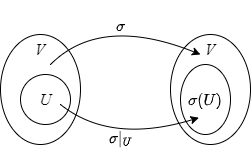
\includegraphics[scale=0.7]{figs/18-1.png}
\end{figure}

但是我们需要注意,\autoref{eq:18:直和分解} 这一分解应当满足一个基本的条件,就是$\sigma$应当把每个$U_i$仍然映射到$U_i$本身,否则我们在讨论$\sigma\vert_{U_i}$的时候它不是一个线性变换,这与我们讨论的主题不一致,即我们希望限制映射$\sigma\vert_{U_i}$是一个线性变换(是$\mathcal{L}(U_i)$中的元素),我们称之为\term{限制线性变换}\index{xianxingbianhuan!xianzhi@限制线性变换 (restriction operator)}.

事实上,满足$\sigma\vert_{U_i}\in\mathcal{L}(U_i)$的子空间$U_i$非常重要,我们需要给予它一个定义:
\begin{definition}
    设$\sigma\in \mathcal{L}(V)$,若$V$的子空间$U$满足$\forall \alpha\in U,\enspace \sigma(\alpha)\in U$,则称$U$是$\sigma$的\term{不变子空间}\index{xianxingkongjian!zi!bubian@不变子空间 (invariant subspace)},或称$U$在$\sigma$下不变,简称为$\sigma$-子空间.
\end{definition}
即不变子空间中的每一个向量经过映射后仍在这一空间中,因此这里的``不变''的含义也是非常直观的. 根据定义我们可以验证或者求解一些很简单的不变子空间. 教材例5.3给出了四个常见的不变子空间的例子,分别是两个平凡子空间和映射的像与核,验证非常简单,此处不赘述. 教材8.20还给出了$p$为多项式时,$\ker p(\sigma)$和$\im p(\sigma)$也为$\sigma$的不变子空间. 我们这里也简要书写一下,供读者熟悉如何利用定义验证不变子空间:
\begin{example}
    若$\sigma\in\mathcal{L}(V)$且$p\in\mathbf{F}[x]$为多项式,则$\ker p(\sigma)$和$\im p(\sigma)$在$\sigma$下不变.
\end{example}

\begin{proof}
    我们只需验证$\ker p(\sigma)$和$\im p(\sigma)$中的元素经过$\sigma$映射后仍在这一空间中即可.
    \begin{enumerate}
        \item $\forall \alpha\in \ker p(\sigma),\enspace p(\sigma)\alpha=0$,因此
              \[(p(\sigma))(\sigma(\alpha))=\sigma(p(\sigma)\alpha)=\sigma(0)=0,\]
              即$\sigma(\alpha)\in \ker p(\sigma)$,因此$\ker p(\sigma)$在$\sigma$下不变;

        \item $\forall \alpha\in \im p(\sigma),\enspace \exists \beta\in V,\enspace \alpha=p(\sigma)\beta$,因此
              \[\sigma(\alpha)=\sigma(p(\sigma)\beta)=p(\sigma)(\sigma(\beta))\in \im p(\sigma),\]
              即$\im p(\sigma)$在$\sigma$下不变.
    \end{enumerate}
    事实上,对于$\ker p(\sigma)$,我们有
    \[ p(\sigma)(\alpha)=p(\sigma)\alpha=p(\sigma(\alpha))=p(0)=0,\]
    因此$\sigma(\alpha)\in \ker p(\sigma)$,即$\ker p(\sigma)$在$\sigma$下不变. 对于$\im p(\sigma)$,我们有
    \[\forall \alpha\in \im p(\sigma),\enspace \exists \beta\in V,\enspace \alpha=p(\sigma)\beta,\]
    因此
    \[\sigma(\alpha)=\sigma(p(\sigma)\beta)=p(\sigma)\sigma(\beta)\in \im p(\sigma),\]
    即$\im p(\sigma)$在$\sigma$下不变.
\end{proof}


\vspace{2ex}
\centerline{\heiti \Large 内容总结}

本节我们重点讨论了线性映射像空间和核空间之间的关联,核心定理就是线性映射基本定理,一方面其证明使用的``设小扩大''的思想十分常见,另一方面它的结论也是相当重要的,它将线性映射的核空间和像空间的维数联系起来,是将来讨论线性方程组一般理论的重要工具,也可以由此导出出发空间、到达空间维数相同时,单射、满射、双射的关联. 除此之外,我们也基于像空间、核空间本身的性质讨论了它们更为复杂的关联,在这些结论的证明中我们能掌握很多基本技巧,如基于像空间、核空间定义的直和的证明、包含关系的证明等,并且综合利用了线性空间维数公式以及本讲介绍的线性映射基本定理,因此很适合作为加深对概念、方法理解运用的例子.

最后我们讨论了线性空间同构的概念,同构映射保持线性相关性的特点,以及通过维数判定有限维线性空间同构的简便方法. 同构是线性空间之间的等价关系,它将线性空间按维数划分为不同的等价类,从而将任意$n$维线性空间的研究转化为对向量空间$\mathbf{R}^n$的研究——事实上本节最后一个例子中构造同构映射的方法就已经体现了这一点的优越性. 同时这也表明线性空间结构的最关键因素就是维数,线性空间之间最本质的差别就是维数不同——这便回应了上一讲开头引言部分的问题. 一组基中的元素是向量还是多项式还是函数并不重要,重要的是只要它们维数相同,我们就可以遮蔽掉元素的差别——因为它们都可以通过坐标映射同构于$\mathbf{R}^n$,因此一切线性空间在坐标作用下都变成了向量空间,变成了最直观的可以用一个一个数字写出来的向量,我们便可以基于此将所有无论多么抽象的线性映射也表示成能用一个一个数字写出来的东西——这就是矩阵. 在有了线性映射的矩阵表示后,我们便可以将抽象的研究都转化为具象的矩阵运算,这一思想我们将在介绍完需要的工具——矩阵运算以及行列式之后深入讨论,届时我们将分别以抽象的线性映射理论和矩阵理论叙述大量的结论,探寻利用二者研究线性代数问题的过程的关联与差异.

\vspace{2ex}
\centerline{\heiti \Large 习题}

\vspace{2ex}
It is not so much whether a theorem is useful that matters, but how elegant it is.
\begin{flushright}
    ——S.Ulam
\end{flushright}

\centerline{\heiti A组}
\begin{enumerate}
    \item 证明:同构映射的逆、复合仍然是同构映射.
\end{enumerate}

\centerline{\heiti B组}
\begin{enumerate}
    \item 设$\sigma(p(x))=p'(x)$(求导),$\forall p(x) \in \mathbf{R}[x]_n$.
          \begin{enumerate}
              \item 证明:$\sigma$是$\mathbf{R}[x]_n$上的线性变换;

              \item 求$\sigma$的值域和$r(\sigma)$,说明$\sigma$是否可逆;

              \item 求$\sigma$的核及其维数;

              \item 求$r(\sigma)+\dim\ker\sigma$,问:$\mathbf{R}[x]_n=\ker\sigma+\im \sigma$是否成立.
          \end{enumerate}

    \item 设$V$为有限维线性空间,$T\in \mathcal{L}(V,V)$且$T$不是恒等变换也不是零变换,问:下列情况是否可能发生?如果可能请举例,不可能请说明理由.
          \begin{enumerate}
              \item $\im T \cap \ker T = \{0\}$;

              \item $\im T \subseteq \ker T$;

              \item $\ker T = \im T$;

              \item $\ker T \subseteq \im T$.
          \end{enumerate}

    \item 若$\sigma_1,\sigma_2\in \mathcal{L}(V,V)$,判断下列说法是否正确,正确请给出证明,反之给出反例:
          \begin{enumerate}
              \item 由$r(\sigma)+\dim\ker\sigma=n$可知$V=\ker\sigma+\im \sigma$;

              \item 若有$\im T \cap \ker T = \{0\}$,则$V=\ker\sigma+\im \sigma$成立;

              \item 因为$\forall \alpha \in V$有$(\sigma_1+\sigma_2)(\alpha)=\sigma_1(\alpha)+\sigma_2(\alpha)$,所以$(\sigma_1+\sigma_2)(V)=\sigma_1(V)+\sigma_2(V)$;

              \item $(I-\sigma)(V)+\sigma(V)=V$,其中$I$为恒等映射.
          \end{enumerate}

    \item 已知$V$为有限维线性空间,$\sigma\in \mathcal{L}(V,V)$,且$\ker\sigma=\im \sigma$,证明:
          \begin{enumerate}
              \item $n$为偶数;

              \item 存在$V$的一组基$\alpha_1,\ldots,\alpha_n$使得
                    \[\sigma(\alpha_1,\ldots,\alpha_n)=(\alpha_1,\ldots,\alpha_n)\begin{pmatrix}
                            0 & E_{\frac{n}{2}} \\ 0 & 0
                        \end{pmatrix}.\]
          \end{enumerate}

    \item 设$V(\mathbf{R})$是线性空间,$\sigma$是$V(\mathbf{R})$到$\mathbf{R}^3$的同构映射,且$\sigma(\alpha_1)=(1,0,1),\enspace\allowbreak\sigma(\alpha_2)=(-2,1,0),\enspace\allowbreak\sigma(\alpha_3)=(-3,2,1),\enspace\allowbreak\sigma(\alpha_4)=(1,1,2)$.
          \begin{enumerate}
              \item $\alpha_1$在$\spa(\alpha_2,\alpha_3)$中吗?

              \item 设$W_1=\spa(\alpha_1,\alpha_2),\enspace W_2=\spa(\alpha_3,\alpha_4)$,求$W_1\cap W_2$.
          \end{enumerate}

    \item 设$c_1,c_2,\ldots,c_n$是$n$个互异的实常数. 证明:$\mathbf{R}[x]_n$到$\mathbf{R}$的一个映射$\sigma$:
          \[\sigma(p(x))=(p(c_1),p(c_2),\ldots,p(c_n))\]
          是$\mathbf{R}[x]_n$到$\mathbf{R}$的一个同构映射.

    \item 设$\sigma$和$\tau$分别为有限维线性空间$U\to V$和$V\to W$的线性映射,证明
          \[\dim\ker\sigma+\dim(\im\sigma\cap\ker\sigma)=\dim\ker(\tau\sigma).\]
\end{enumerate}

\centerline{\heiti C组}
\begin{enumerate}
    \item 设$V$是一个$n$维线性空间,$V=W_1\oplus W_2,\enspace\sigma\in \mathcal{L}(V,V)$. 证明:$\sigma$可逆$\iff V=\sigma(W_1)+\sigma(W_2)$.

    \item 设$V_1,V_2,V_3$分别为$m,n,s$维线性空间,$\sigma\in \mathcal{L}(V_1,V_2),\enspace\tau\in \mathcal{L}(V_2,V_3)$,则
          \[r(\sigma)+r(\tau)-n \leqslant r(\tau\sigma) \leqslant \min\{r(\sigma),r(\tau)\}.\]

    \item 设$V_1$是有线维线性空间,$\sigma,\tau\in \mathcal{L}(V_1,V_2)$,则
          \[r(\sigma+\tau) \leqslant r(\sigma)+r(\tau).\]

          事实上前两题的结论在下一章节矩阵的秩中都会涉及,此处有兴趣的同学可以尝试从线性映射的角度理解这两个秩不等式. 由于这是教材中小字部分内容,一般而言不在考察范围,如果出现且无法找到合适方式,可以考虑化为矩阵进行证明.

    \item 设$\sigma\in \mathcal{L}(V,V)$,$\dim V_1=n$,且$\sigma^2=\sigma$,$I$是$V$上的恒等变换. 证明:
          \begin{enumerate}
              \item $(I-\sigma)(V) \in \ker\sigma$;

              \item $r(I-\sigma)+r(\sigma)=n$.
          \end{enumerate}

    \item 已知$V$为有限维线性空间,$\sigma\in \mathcal{L}(V,V)$,且$\sigma^2=\theta$(零映射). 证明:
          \begin{enumerate}
              \item $\sigma$的像空间维数不超过$\dfrac{n}{2}$;

              \item 设$A$是$\sigma$在某组基下的矩阵,则方程组$AX=0$的基础解系至少有$\dfrac{n}{2}$个解.
          \end{enumerate}
\end{enumerate}

\chapter{矩阵运算基础}

上一节我们将前面逐步搭建的线性空间与线性映射的抽象转变为具象的表达——矩阵——这是我们上一节最后内容总结中提到的利用坐标映射同构到最简单的向量空间的优越性的体现. 从本讲起的三讲内容中,我们的目光都会聚焦于具象的矩阵,但我们的视角时常会结合线性映射同步进行. 本讲我们首先介绍矩阵的基本运算的定义(及其与线性映射的关联)、性质与基本技巧,之后我们会在此基础上从线性映射的秩出发定义矩阵的秩,得到第一个重要的矩阵标准形——相抵标准形. 最后我们会更进一步加强运算技巧,介绍一些在解题或者是实际应用中常用的矩阵运算技巧.

\section{矩阵乘法}

\subsection{矩阵乘法的定义与基本性质}

我们在前文证明过线性映射的复合仍然是线性映射,当我们写出 $(\tau{\color{lightgray}\circ}\sigma)(\alpha) = \tau(\sigma(\alpha))$ 时我们通过映射复合定义了映射的乘法(只有这样才能在形式上说结合律成立). 于是矩阵作为一种特殊的映射,其乘法应当继承自矩阵的复合,我们注意到映射 $\tau\sigma$ 能够存在的条件是 $\tau$ 的出发空间和 $\sigma$ 的到达空间相同,即两个映射可以通过一个公共的中间空间``连接''起来
\[
    \tikzcdset{arrow style=tikz, diagrams={>=stealth}}
    \begin{tikzcd}
        V_1 \arrow[r, "\sigma"] \arrow[rr, bend right, "\tau{\color{lightgray}{}\circ{}}\sigma"'] & V_2 \arrow[r, "\tau"] & V_3
    \end{tikzcd}
\]

我们假设读者已经熟知映射的相乘即复合,在后文中我们将会省去映射复合的符号 ${\color{lightgray}\circ}$.  那么将 $V_1, V_2, V_3$ 分别替换为我们熟悉的 $\mathbf{F}^n, \mathbf{F}^m, \mathbf{F}^p$,我们就理应能够将 $p\times m$ 和 $m\times n$ 的两个矩阵相乘
\[
    \tikzcdset{arrow style=tikz, diagrams={>=stealth}}
    \begin{tikzcd}
        \mathbf{F}^n \arrow[r, "B"] \arrow[rr, bend right, "AB"'] & \mathbf{F}^m \arrow[r, "A"] & \mathbf{F}^p
    \end{tikzcd}
\]

由于复合的映射的复合是线性映射,那么矩阵的乘法应该给出一个矩阵 $AB\in\mathbf{F}^{p\times n}$. 那么让我们动手计算一下
\begin{align*}
    (AB)(x) &= A(Bx) \\
    &= \begin{pmatrix}
        a_{11} & a_{12} & \cdots & a_{1m} \\
        a_{21} & a_{22} & \cdots & a_{2m} \\
        \vdots & \vdots & \ddots & \vdots \\
        a_{p1} & a_{p2} & \cdots & a_{pm}
    \end{pmatrix} \left( \begin{pmatrix}
        b_{11} & b_{12} & \cdots & b_{1n} \\
        b_{21} & b_{22} & \cdots & b_{2n} \\
        \vdots & \vdots & \ddots & \vdots \\
        b_{m1} & b_{m2} & \cdots & b_{mn}
    \end{pmatrix} \begin{pmatrix}
        x_1 \\ x_2 \\ \cdots \\ x_n
    \end{pmatrix} \right)\\
    &= \begin{pmatrix}
        a_{11} & a_{12} & \cdots & a_{1m} \\
        a_{21} & a_{22} & \cdots & a_{2m} \\
        \vdots & \vdots & \ddots & \vdots \\
        a_{p1} & a_{p2} & \cdots & a_{pm}
    \end{pmatrix} \begin{pmatrix}
        \sum_{j=1}^n b_{1j} x_j \\
        \sum_{j=1}^n b_{2j} x_j \\
        \vdots \\
        \sum_{j=1}^n b_{mj} x_j
    \end{pmatrix} \\
    &= \begin{pmatrix}
        \sum_{k=1}^m a_{1k} b_{kj} x_j \\
        \sum_{k=1}^m a_{2k} b_{kj} x_j \\
        \vdots \\
        \sum_{k=1}^m a_{pk} b_{kj} x_j
    \end{pmatrix} \\
    &= \begin{pmatrix}
        \sum_{k=1}^m a_{1k} b_{k1} & \sum_{k=1}^m a_{1k} b_{k2} & \cdots & \sum_{k=1}^m a_{1k} b_{kn} \\
        \sum_{k=1}^m a_{2k} b_{k1} & \sum_{k=1}^m a_{2k} b_{k2} & \cdots & \sum_{k=1}^m a_{2k} b_{kn} \\
        \vdots & \vdots & \ddots & \vdots \\
        \sum_{k=1}^m a_{pk} b_{k1} & \sum_{k=1}^m a_{pk} b_{k1} & \cdots & \sum_{k=1}^m a_{pk} b_{kn}
    \end{pmatrix} \begin{pmatrix}
        x_1 \\ x_2 \\ \vdots \\ x_n
    \end{pmatrix}\\
\end{align*}

设 $C = AB$,则矩阵相乘结果中有
\[
    c_{ij} = \sum_{k=1}^m a_{ik} b_{kj}
\]

矩阵乘法 $AB$ 表现为 $A$ 的行和 $B$ 的列的点乘,于是我们可以给出矩阵乘法的定义:
\begin{definition}{}{}
    设$A=(a_{ij})_{p\times m},B=(b_{ij})_{m\times n}$,我们定义$A$与$B$的乘积矩阵$C=AB=(c_{ij})_{p\times n}$是一个$p\times n$矩阵,其中它的第$i$行第$j$列元素为矩阵$A$的第$i$行与矩阵$B$的第$j$列对应位置元素相乘后求和的结果,即
    \[
        c_{ij}
        =\sum_{k=1}^m a_{ik} b_{kj}
        =a_{i1}b_{1j}+a_{i2}b_{2j}+\cdots+a_{im}b_{mj}\enspace(i=1,\ldots,p,\enspace j=1,\ldots,n).
    \]
\end{definition}

这一定义带给我们的感受与我们在上一讲定义矩阵加法和数乘时的直观不同,如果脱离了映射复合的背景,在我们初看这一定义时必然会产生一个疑惑:为什么矩阵乘法定义得如此复杂,为什么不定义成两个矩阵对应元素相乘就可以了呢?事实上,只有这么定义,才能使结合律 $(AB)x = A(Bx)$ 在形式上变为可能,如果从输入第 $j$ 个分量对输出第 $i$ 个分量的权重来看,输入的第 $j$ 个分量可以通过 $b_{kj}, \enspace 1\leqslant k\leqslant m$ 对中间变量产生影响,而中间变量对输出第 $i$ 个分量的影响体现在 $a_{ik}, \enspace 1\leqslant k\leqslant m$,相乘时就必须要把这些影响对中间变量的每一项叠加起来,所以是 $a_{ik} b_{kj}$ 对 $k$ 的求和,最终导致了输入和输出指标固定,对中间指标求和. 如果从基的角度看:

\begin{enumerate}
    \item 设线性空间 $V_1(F), V_2(F), V_3(F)$ 的基分别为
    \begin{align*}
        B_1&=\{\varepsilon, \varepsilon_2,\ldots,\varepsilon_n\},
        B_2&=\{\zeta_1,\zeta_2,\ldots,\zeta_m\},
        B_3&=\{\eta_1,\eta_2,\ldots,\eta_p\}
    \end{align*}
    $\sigma \in L(V_1,V_2), \tau \in L(V_2,V_3)$,且 $\sigma, \tau$ 分别关于基 $B_1$ 和 $B_2$ 及基 $B_2$ 和 $B_3$ 的矩阵为 $B=(b_{i,j})_{m \times n}$ 和 $A=(a_{ij})_{p\times m}$,即:

          $M(\tau)=A=\begin{pmatrix}
                  a_{11} & a_{12} & \cdots & a_{1m} \\
                  a_{21} & a_{22} & \cdots & a_{2m} \\
                  \vdots & \vdots & \ddots & \vdots \\
                  a_{p1} & a_{p2} & \cdots & a_{pm}
              \end{pmatrix}$,
          $M(\sigma)=B=\begin{pmatrix}
                  b_{11} & b_{12} & \cdots & b_{1n} \\
                  b_{21} & b_{22} & \cdots & b_{2n} \\
                  \vdots & \vdots & \ddots & \vdots \\
                  b_{m1} & b_{m2} & \cdots & b_{mn}
              \end{pmatrix}$.

    \item 则 $\tau\sigma \in L(V_1,V_3)$ 关于基 $B_1$ 和 $B_3$ 的矩阵 $C=(c_{ij})_{p\times n}$ 中第 $j$ 列元素 $c_{1j},c_{2j},\ldots,c_{pj}$ 是 $\tau\sigma(\varepsilon_j)$ 在基 $B_3$ 下的坐标. 于是有:
          \begin{align*}
            \tau\sigma(\varepsilon_j)
            &=\tau(\sigma(\varepsilon_j))
            &=\tau\left(\sum_{k=1}^{m}b_{kj}\zeta_k\right) \\
            &=\sum_{k=1}^{m}b_{kj}\tau(\zeta_k) \\
            &=\sum_{k=1}^{m}b_{kj}\left(\sum_{i=1}^{p}a_{ik}\eta_i\right) \\
            &=\sum_{i=1}^{p}\left(\sum_{k=1}^{m}a_{ik}b_{kj}\right)\eta_i
          \end{align*}

          即得:$c_{ij}=a_{i1}b_{1j}+a_{i2}b_{2j}+\cdots+a_{im}b_{mj}$. 换言之,表示矩阵的乘积等于乘积(复合)的表示矩阵,这也可以通过映射的复合得到简单的验证
          \begin{align*}
            \mathbf{M}_{\color{lightgray} B_2, B_3} (\tau) \mathbf{M}_{\color{lightgray} B_1, B_2} (\sigma)
            &= (B_3^{-1} \tau B_2) (B_2^{-1} \sigma B_1) \\
            &= B_3^{-1} \tau (B_2 B_2^{-1}) \sigma B_1 \\
            &= B_3^{-1} (\tau \sigma) B_1 \\
            &= \mathbf{M}_{\color{lightgray} B_1, B_3} (\tau \sigma)
          \end{align*}

          如果从交换图的视角看,我们可以通过绘制箭头简单地看出,根据映射复合构造出的三个表示矩阵显然满足 $\mathbf{M}_{\color{lightgray} B_2, B_3} (\tau) \mathbf{M}_{\color{lightgray} B_1, B_2} (\sigma) = \mathbf{M}_{\color{lightgray} B_1, B_3} (\tau \sigma)$:
          \[
            \tikzcdset{arrow style=tikz, diagrams={>=stealth}}
            \begin{tikzcd}
                V_1
                    \arrow[rr, "\sigma"]
                    \arrow[rrrr, bend left, "\tau\sigma"]
                    \arrow[d, shift left, lightgray, "B_1^{-1}"]
                && V_2
                    \arrow[rr, "\tau"]
                    \arrow[d, shift left, lightgray, "B_2^{-1}"]
                && V_3
                    \arrow[d, shift left, lightgray, "B_3^{-1}"]
                \\ \mathbf{F}^n
                    \arrow[u, shift left, "B_1"]
                    \arrow[rrrr, bend right, "\mathbf{M}_{\color{lightgray} B_1, B_3} (\tau\sigma)"']
                    \arrow[rr, "\mathbf{M}_{\color{lightgray} B_1, B_2} (\sigma)"']
                && \mathbf{F}^m
                    \arrow[u, shift left, "B_2"]
                    \arrow[rr, "\mathbf{M}_{\color{lightgray} B_2, B_3} (\tau)"']
                && \mathbf{F}^p
                    \arrow[u, shift left, "B_3"]
            \end{tikzcd}
          \]

          但是需要注意的是,这要求在两个映射矩阵表示的基底选择中,$V_2$ 选取的基底是相同的,否则这个过程就会失败,基底不同时我们就无法写出 $\mathbf{M}(\tau)\mathbf{M}(\sigma) = \mathbf{M}(\tau\sigma)$
          \[
            \tikzcdset{arrow style=tikz, diagrams={>=stealth}}
            \begin{tikzcd}
                & V_1
                    \arrow[rd, "\sigma"]
                    \arrow[rr, "\tau\sigma"]
                    \arrow[dl, shift left, lightgray, "B_1^{-1}"]
                && V_3
                    \arrow[dr, shift left, lightgray, "B_3^{-1}"]
                \\ \mathbf{F}^n
                    \arrow[ur, shift left, "B_1"]
                    \arrow[rrrr, bend right=90, "\mathbf{M}_{\color{lightgray} B_1, B_3} (\tau\sigma)"']
                    \arrow[rd, "\mathbf{M}_{\color{lightgray} B_1, B_2} (\sigma)"']
                && V_2
                    \arrow[ur, "\tau"]
                    \arrow[dl, shift left, lightgray, "B_2^{-1}"]
                    \arrow[dr, shift left, lightgray, "(B_2')^{-1}"]
                && \mathbf{F}^p
                    \arrow[ul, shift left, "B_3"]
                \\ & \mathbf{F}^m
                    \arrow[ur, shift left, "B_2"]
                    \arrow[rr, dashed, "?"']
                && \mathbf{F}^m
                    \arrow[ul, shift left, "B_2'"]
                    \arrow[ur, "\mathbf{M}_{\color{lightgray} B_2', B_3} (\tau)"']
            \end{tikzcd}
          \]
\end{enumerate}

接下来我们再给出两个线性映射的例子来理解矩阵乘法:
\begin{enumerate}
    \item 回顾上一节中提到的旋转$\theta$角的线性映射对应的矩阵$M_{\theta}=\begin{pmatrix}
                  \cos\theta & -\sin\theta \\
                  \sin\theta & \cos\theta
              \end{pmatrix}$. 我们考虑先旋转$\theta_1$,然后旋转$\theta_2$对应的两个变换$\sigma_1,\sigma_2$的复合$\sigma_2\sigma_1$,实际上就是旋转$\theta_1+\theta_2$角度,其矩阵表示为$M_{\theta_1+\theta_2}$,而矩阵乘法
          \begin{align*}
              M_{\theta_2}M_{\theta_1}
               & =\begin{pmatrix}
                      \cos\theta_2 & -\sin\theta_2 \\
                      \sin\theta_2 & \cos\theta_2
                  \end{pmatrix}\begin{pmatrix}
                                   \cos\theta_1 & -\sin\theta_1 \\
                                   \sin\theta_1 & \cos\theta_1
                               \end{pmatrix} \\
               & =\begin{pmatrix}
                      \cos\theta_2\cos\theta_1-\sin\theta_2\sin\theta_1 & -\cos\theta_2\sin\theta_1-\sin\theta_2\cos\theta_1 \\
                      \sin\theta_2\cos\theta_1+\cos\theta_2\sin\theta_1 & -\sin\theta_2\sin\theta_1+\cos\theta_2\cos\theta_1
                  \end{pmatrix} \\
               & =\begin{pmatrix}
                      \cos(\theta_1+\theta_2) & -\sin(\theta_1+\theta_2) \\
                      \sin(\theta_1+\theta_2) & \cos(\theta_1+\theta_2)
                  \end{pmatrix}=M_{\theta_1+\theta_2},
          \end{align*}
          这表明矩阵乘法$M_{\theta_2}M_{\theta_1}$的结果确实与$\sigma_2\sigma_1$的矩阵表示$M_{\theta_1+\theta_2}$一致.

    \item 我们在此再次强调矩阵相乘时左侧矩阵的列数应该等于右边矩阵的行数:回顾线性映射的复合,若复合$\sigma_1\sigma_2$符合定义,则必须有$\sigma_2$的到达空间恰好是$\sigma_1$的出发空间,故两空间维数一致,那么$\sigma_1$对应的矩阵$A$的列数和$\sigma_2$对应的矩阵$B$的行数一致,这也是我们要求两个矩阵$A,B$可乘的重要条件的来源. 而最后乘法的结果行数等于$A$的行数,列数等于$B$的列数,这也与$\sigma_1\sigma_2$出发空间为$\sigma_2$出发空间(对应于$B$的列数),到达空间为$\sigma_1$到达空间(对应于$A$的行数)一致.
\end{enumerate}

\begin{example}{}{}
    设$A=\begin{pmatrix}
            1 & 0 & -1 \\
            1 & 1 & -3
        \end{pmatrix}, B=\begin{pmatrix}
            0 & 3 \\
            1 & 2 \\
            3 & 1
        \end{pmatrix}$,求$AB$和$BA$.
\end{example}

\begin{solution}
    $AB =\begin{pmatrix}
            0-3 & 3-1   \\
            1-9 & 3+2-3
        \end{pmatrix}=\begin{pmatrix}
            -3 & 2 & -8 & 2
        \end{pmatrix}$,

    $BA=\begin{pmatrix}
            0+3 & 0+3 & 0-9  \\
            1+2 & 0+2 & -1-6 \\
            3+1 & 0+1 & -3-3
        \end{pmatrix}=\begin{pmatrix}
            3 & 3 & -9 \\
            3 & 2 & -7 \\
            4 & 1 & -6
        \end{pmatrix}$.
\end{solution}

接下来给出矩阵运算的几个基本性质:
\begin{enumerate}
    \item $(AB)C=A(BC)$(结合律)

    \item $\lambda(AB)=(\lambda A)B=A(\lambda B),\enspace \lambda \in \mathbf{F}$

    \item $A(B+C)=AB+AC$(左分配律)

    \item $(B+C)P=BP+CP$(右分配律)
\end{enumerate}
证明方法十分简单:使用映射的结合律、线性性和分配律直接证明对应的几何版本的正确性,或者直接暴力设出矩阵元素然后暴力计算证明等号两边对应位置(如第$i$行第$j$列元素)相等也是可行的.

实际上,由矩阵加法和乘法满足的运算律可知,全体$n$阶方阵构成的集合$\mathbf{F}^{n\times n}$关于矩阵加法和乘法构成环.

在本节最后,我们有四个非常重要的问题需要仔细探讨:
\begin{enumerate}
    \item 在有了矩阵乘法的定义后,高斯消元法中我们将线性方程组简记为$AX=b$实际上是相当自然的,除此之外,我们将向量坐标表示为列向量的形式,例如将向量 $v$ 对基 $\alpha$ 分解
          \[v=(\alpha_1,\alpha_2,\ldots,\alpha_n)\begin{pmatrix}
                  x_1 \\ x_2 \\ \vdots \\ x_n
              \end{pmatrix}\]
          这也是符合矩阵形式乘法定义的一种习惯(虽然基一般不是数域$\mathbf{F}$或者向量空间$\mathbf{F}^m$中的元素).

    \item 事实上,在这里我们可以看出求解线性方程组和线性映射之间的关联. 我们设$AX=b$的解为
          \[X=\begin{pmatrix}
                  x_1 \\ x_2 \\ \vdots \\ x_n
              \end{pmatrix}\]
          由$AX=b$和线性映射矩阵表示,我们有
          \begin{equation}\label{eq:7:方程组与核空间1}
              (\sigma(\varepsilon_1),\sigma(\varepsilon_2),\ldots,\sigma(\varepsilon_n))\begin{pmatrix}
                  x_1 \\ x_2 \\ \vdots \\ x_n
              \end{pmatrix}=(\alpha_1,\alpha_2,\ldots,\alpha_m)A\begin{pmatrix}
                  x_1 \\ x_2 \\ \vdots \\ x_n
              \end{pmatrix}=b
          \end{equation}
          即$x_1\sigma(\varepsilon_1)+x_2\sigma(\varepsilon_2)+\cdots+x_n\sigma(\varepsilon_n)=b$,即
          \begin{equation}\label{eq:7:方程组与核空间2}
              \sigma(x_1\varepsilon_1+x_2\varepsilon_2+\cdots+x_n\varepsilon_n)=b.
          \end{equation}
          由此我们将线性方程组的求解问题和找到线性映射到达空间中某个向量在出发空间中原像的坐标联系起来了,即将求解$AX=b$和求解$\sigma(a)=b$联系起来了,只是我们求解后者时通常是对于一般的向量空间而言的,这时求解是通过求出$a$在矩阵表示基下的坐标实现的.

          若前述$b=0$,则我们将齐次线性方程组的解空间与线性映射的核空间联系起来了,即线性映射的核空间中元素在一组基下的向量就是这一线性映射在这组基下的矩阵表示作为系数矩阵的线性方程组的解. 这一联系将在\nameref{chap:朝花夕拾}中有更深入的讨论.

    \item 我们可以更进一步理解矩阵乘法. 假设矩阵$A=(a_{ij})_{m\times n}$与$B=(b_{ij})_{n\times l}$相乘,我们有如下结论:
          \begin{enumerate}
              \item 乘积的第$k$列等于$A$乘以$B$的第$k$列,乘积的第$j$行等于$A$的第$j$行乘以$B$,这一点根据矩阵乘法计算方式显然,我们可以利用这一性质证明下面例子的结论:
                    \begin{example}{}{}
                        设$A,B$都是由非负实数组成的矩阵且$AB$有一行等于0,证明:或者$A$有一行为0,或者$B$有一行为0.
                    \end{example}
                    \begin{proof}
                        设$A=(a_{ij})_{m\times n}$,$B=(b_{ij})_{n\times l}$,且设$AB=(c_{ij})_{m\times l}$的第$i$行为0,则根据前面的讨论可知就是$A$的第$i$行乘以$B$得到了全0行向量. 因此若$A$的第$i$行为0,则结论成立;否则$A$的第$i$行中存在某个元素大于0,不妨设$a_{ik}>0$,则此时$B$的第$k$行各元素必须均为0,否则若$b_{kj}>0$,我们有
                        \[c_{ij}=a_{i1}b_{1j}+\cdots+a_{ik}b_{kj}+\cdots+a_{in}b_{nj}>0,\]
                        综上可知结论成立.
                    \end{proof}

              \item 乘积的每一列都是矩阵$A$各列的线性组合,每一行都是矩阵$B$各行的线性组合. 我们简要说明前者,后者理由类似. 我们考察乘积的每一列,由1可知乘积的第$k$列等于$A$乘以$B$的第$k$列,我们展开写乘积矩阵$C=(c_{ij})_{m\times l}$第$k$列的结果:
                    \begin{align*}
                        c_{1k} & =a_{11}b_{1k}+a_{12}b_{2k}+\cdots+a_{1n}b_{nk} \\
                        c_{2k} & =a_{21}b_{1k}+a_{22}b_{2k}+\cdots+a_{2n}b_{nk} \\
                               & \vdotswithin{=}                                \\
                        c_{mk} & =a_{m1}b_{1k}+a_{m2}b_{2k}+\cdots+a_{mn}b_{nk}
                    \end{align*}
                    我们将上面的行进行组合,写成列向量形式,即
                    \[\begin{pmatrix}
                            c_{1k} \\ c_{2k} \\ \vdots \\ c_{mk}
                        \end{pmatrix}=b_{1k}\begin{pmatrix}
                            a_{11} \\ a_{21} \\ \vdots \\ a_{m1}
                        \end{pmatrix}+b_{2k}\begin{pmatrix}
                            a_{12} \\ a_{22} \\ \vdots \\ a_{m2}
                        \end{pmatrix}+\cdots+b_{nk}\begin{pmatrix}
                            a_{1n} \\ a_{2n} \\ \vdots \\ a_{mn}
                        \end{pmatrix}\]
                    由此我们将乘积的列表示成了矩阵$A$各列的线性组合.
          \end{enumerate}

    \item 之后我们会经常看见两种记号,即
          \begin{align*}
              (\sigma(\varepsilon_1),\sigma(\varepsilon_2),\ldots,\sigma(\varepsilon_n))
              & =(\alpha_1,\alpha_2,\ldots,\alpha_m)A \\
              \sigma(\varepsilon_1,\varepsilon_2,\ldots,\varepsilon_n)
              & =(\alpha_1,\alpha_2,\ldots,\alpha_m)A
          \end{align*}
          教材中两个记号是等价的,这只是记号上的差别,含义完全相同. 但是在之后我们还会看到一个很特别的书写方式
          \[
            (\sigma(\varepsilon_1,\varepsilon_2,\ldots,\varepsilon_n))B
            =\sigma((\varepsilon_1,\varepsilon_2,\ldots,\varepsilon_n)B)
          \]
          教材不加解释地使用了这一等式,这容易导致读者的困惑,因此我们这里简要说明它们的确是等价的,从而接下来读者可以放心地自由使用这一结论.

          根据上述的第一个性质可知,我们只需要证明对$B$的某一列上式成立即可,因为乘法结果是列与列对应的. 我们设$B$的第$k$列为
          \[B_k=\begin{pmatrix}
                  b_{1k} \\ b_{2k} \\ \vdots \\ b_{nk}
              \end{pmatrix}\]
          则
          \begin{align*}
              (\sigma(\varepsilon_1,\varepsilon_2,\ldots,\varepsilon_n))
              \begin{pmatrix}
                  b_{1k} \\ b_{2k} \\ \vdots \\ b_{nk}
              \end{pmatrix}
               & =(\sigma(\varepsilon_1),\sigma(\varepsilon_2),\ldots,\sigma(\varepsilon_n))\begin{pmatrix}
                                                                                                b_{1k} \\ b_{2k} \\ \vdots \\ b_{nk}
                                                                                            \end{pmatrix} \\
               & =b_{1k}\sigma(\varepsilon_1)+b_{2k}\sigma(\varepsilon_2)+\cdots+b_{nk}\sigma(\varepsilon_n)                    \\
               & =\sigma(b_{1k}\varepsilon_1+b_{2k}\varepsilon_2+\cdots+b_{nk}\varepsilon_n)                                    \\
               & =\sigma((\varepsilon_1,\varepsilon_2,\ldots,\varepsilon_n)
              \begin{pmatrix}
                  b_{1k} \\ b_{2k} \\ \vdots \\ b_{nk}
              \end{pmatrix})
          \end{align*}
          故得证.
\end{enumerate}

事实上矩阵乘法有很多和数的乘法重要的不同,我们在此特别指出供读者参考:
\begin{enumerate}[label=(\arabic*)]
    \item 矩阵乘法不一定满足交换律(即$AB$不一定等于$BA$,事实上随手写两个矩阵,很大的概率就是不交换的,甚至交换过来不可乘). 因此实数的完全平方公式代入矩阵不一定成立,即很多时候$(A+B)^2=A^2+AB+BA+B^2\neq A^2+2AB+B^2$;

    \item 但是注意数量矩阵(即对角线上元素都相等,其余均为0,单位矩阵是其特例)和任何同阶的矩阵相乘都是可交换的,这一点在矩阵求幂时很有用;

    \item \label{item:7:矩阵乘法:3}
          $A\neq O$且$B\neq O$不能推出$AB\neq O$. 例如线性方程组$AX = 0$有非零解,若$B$的各列均为方程非零解,则$AB = O$ 在环上这种元素通常被称为零因子.

    \item 消去律也不一定满足:即$AB = AC$不一定$A = B$. 原因在于$AB=AC \implies A(B-C)=O$,由 \ref*{item:7:矩阵乘法:3} 可知不一定$B = C$.
\end{enumerate}

\subsection{矩阵多项式}

我们在线性空间中已经介绍过,我们一般用$\mathbf{F}[x]_{m+1}$表示数域$\mathbf{F}$上的次数最高为$m$的多项式全体,其中的元素我们一般记为
\[p(x)=a_mx^m+a_{m-1}x^{m-1}+\cdots+a_1x+a_0,\enspace a_i\in\mathbf{F}\enspace(i=1,2,\ldots,m)\]
我们发现这里的自变量不一定需要是一个数,也可以是线性变换或者方阵,因为只要可以和自己相乘就能定义乘方. 例如线性映射$\sigma:V\to V$构成的$m$次多项式可以记为
\[p(\sigma)=a_m\sigma^m+a_{m-1}\sigma^{m-1}+\cdots+a_1\sigma+a_0I\]
其中$\sigma^i$表示$\sigma$复合$i$次,$I$表示恒等映射. 我们很容易说明当$\sigma$在$V$的一组基下矩阵表示为$A$时,$p(\sigma)$在同一组基下的矩阵表示为
\[p(A)=a_mA^m+a_{m-1}A^{m-1}+\cdots+a_1A+a_0E,\]
其中$E$表示单位矩阵. 由此我们便得到了矩阵多项式的定义,我们有如下几点需要强调:
\begin{enumerate}
    \item 这里我们要求$\sigma$是线性变换(即出发空间和到达空间一致),因为只有满足这一条件才能复合. 对于矩阵而言,其作用在标准 $n$ 维向量空间 $\mathbf{F}^n$ 上,所以矩阵可求幂即要求出发空间和到达空间维数相同即可,这样才能保证矩阵的幂次可以定义(即$A$和$A$可乘,因此$A$的行列数一致);

    \item 上面的定义隐含:$\sigma^0 = I, A^0=E$;

    \item $A^kA^m=A^{k+m},\enspace (A^k)^m=A^{km}$,其中$A$为方阵,$k,m$为任意正整数. 当 $A$ 可逆时这一式可以拓展到全体整数,负整数对应于逆矩阵的情况,接下来可逆的部分会作进一步解释.
\end{enumerate}

\begin{example}{}{}
    展开矩阵多项式$(A+\lambda E)^n$.
\end{example}

\begin{solution}
    由于$A$与$E$是可交换的,并且$A^nE^m=A^n$显然成立,因此我们结合中学学过的二项式展开,得到结果:
    \begin{align*}
        (A+\lambda E)^n & =\sum_{i=0}^nC_n^iA^i(\lambda E)^{n-i}    \\
                        & =\sum_{i=0}^nC_n^i\lambda^{n-i}A^iE^{n-i} \\
                        & =\sum_{i=0}^nC_n^i\lambda^{n-i}A^i.
    \end{align*}
\end{solution}

\begin{example}{}{矩阵多项式可交换}
    设$f(x),g(x) \in \mathbf{F}[x],\enspace A,B \in \mathbf{M}_n(\mathbf{F})$. 证明:
    \begin{enumerate}
        \item $f(A)g(A)=g(A)f(A)$;

        \item 如果$AB=BA$,则$f(A)g(B)=g(B)f(A)$;
    \end{enumerate}
\end{example}

\begin{solution}
    我们可以直接证明第二点,因为第一点是第二点的特例. 设$f(x)=\displaystyle\sum_{i=0}^ma_ix^i$,$g(x)=\displaystyle\sum_{j=0}^sb_jx^j$,$A^0=B^0=E$,则
    \begin{align*}
        f(A)g(B) & =\sum_{i=0}^ma_iA^i\cdot \sum_{j=0}^sb_jB^j\quad(AB=BA)                            \\
                 & =\sum_{k=0}^{m+s}\sum_{i+j=k}a_ib_jA^iB^j=\sum_{k=0}^{m+s}\sum_{i+j=k}b_ja_iB^jA^i \\
                 & =g(B)f(A).
    \end{align*}
    事实上由于$A\cdot A=A\cdot A$,因此$f(A)g(A)=g(A)f(A)$只是上面证明的结论的特例.
\end{solution}

\section{一组例题}

在介绍了矩阵乘法后,我们可以进一步审视线性映射矩阵表示的定义. 我们来看一组初学时可能混淆或者不理解的例子,从而加深对概念的理解:
\begin{example}{}{矩阵表示2}
    设$A=\begin{pmatrix}1 & 0 & 2 \\ -1 & 2 & 1 \\ 1 & 2 & 5\end{pmatrix}$为两个三维线性空间之间的线性映射$\sigma$对应的矩阵,求$\sigma$的像空间和核空间.
\end{example}
(注:本题没有给出线性映射出发空间和到达空间的基,读者可以任意假设.)

\begin{solution}
    求解像空间和核空间,仍然是原先介绍的方法,虽然本题没有给出线性映射的直接定义,但矩阵表示也能给我们足够的信息. 我们设这一矩阵表示的线性映射为$\sigma$,且
    \[(\sigma(\varepsilon_1),\sigma(\varepsilon_2),\sigma(\varepsilon_3))=(\alpha_1,\alpha_2,\alpha_3)A\]
    根据线性映射矩阵表示的定义,我们知道矩阵表示就是线性映射在出发空间一组基下的像在到达空间一组基下的坐标按列排列,因此
    \begin{align*}
        \sigma(\varepsilon_1) & =\alpha_1-\alpha_2+\alpha_3   \\
        \sigma(\varepsilon_2) & =2\alpha_2+2\alpha_3          \\
        \sigma(\varepsilon_3) & =2\alpha_1+\alpha_2+5\alpha_3
    \end{align*}
    因此$\im\sigma=\spa(\alpha_1-\alpha_2+\alpha_3,2\alpha_2+2\alpha_3,2\alpha_1+\alpha_2+5\alpha_3)$,然后求解极大线性无关组即可,结果为$\im\sigma=\spa(\alpha_1-\alpha_2+\alpha_3,2\alpha_2+2\alpha_3)$

    这里求解极大线性无关组的方法我们可以回忆\autoref{ex:转化为坐标},我们先将三个向量转化为到达空间基下坐标,然后求解极大线性无关组,最后把基添加回来即可. 实际上我们会发现,这里的三个坐标就是矩阵$A$的三个列向量(因为矩阵表示就是线性映射在出发空间一组基下的像在到达空间一组基下的坐标按列排列),因此我们只需要求解矩阵$A$的列向量的极大线性无关组$(1,-1,1),(0,2,2)$,然后再将到达空间的基添加回来即可.

    然后求解核空间,我们设$\sigma(\varepsilon)=0$,将$\varepsilon$写成出发空间基的表示后事实上就是\autoref{eq:7:方程组与核空间2} 的形式,我们已说明这一形式与\autoref{eq:7:方程组与核空间1} 等价,因此我们只需求解$AX=0$然后代回出发空间的基即可,最终结果为$\ker\sigma=\spa(4\varepsilon_1+3\varepsilon_2-2\varepsilon_3)$.
\end{solution}

总结一下,此类题目求解像空间实际上就是求出矩阵列向量的极大线性无关组,然后记得将结果对到达空间的基向量做线性组合. 求解核空间只需求解齐次线性方程组$AX=0$并将解对出发空间的基向量即可.

\begin{example}{}{矩阵表示3}
    已知3阶矩阵$A=\begin{pmatrix}
            1 & 0 & 1 \\ 0 & -1 & 0 \\ -1 & 1 & -1
        \end{pmatrix}$. 定义$\mathbf{R}^{3 \times 3}$上的线性变换$\sigma(X)=AX,\enspace X \in \mathbf{R}^{3 \times 3}$. 求$\sigma$的像和核.
\end{example}

\begin{solution}
    核空间求解较为简单,我们先求解核空间. 我们首先求解线性方程组$AY=0$,其中$Y$为列向量,解得其基础解系为$\eta=(1,0,-1)^\mathrm{T}$.

    记$X=(X_1,X_2,X_3)$,则$X\in\ker\sigma$即$AX=(AX_1,AX_2,AX_3)=O$,即$AX_1=AX_2=AX_3=0$,因此$X_1,X_2,X_3$都能由$\eta$线性表出,故
    \[X=(k_1\eta,k_2\eta,k_3\eta)=\begin{pmatrix}
            k_1 & k_2 & k_3 \\ 0 & 0 & 0 \\ -k_1 & -k_2 & -k_3
        \end{pmatrix},\enspace k_1,k_2,k_3\in\mathbf{R},\]
    即$X=k_1\begin{pmatrix}
            1 & 0 & 0 \\ 0 & 0 & 0 \\ -1 & 0 & 0
        \end{pmatrix}+k_2\begin{pmatrix}
            0 & 1 & 0 \\ 0 & 0 & 0 \\ 0 & -1 & 0
        \end{pmatrix}+k_3\begin{pmatrix}
            0 & 0 & 1 \\ 0 & 0 & 0 \\ 0 & 0 & -1
        \end{pmatrix}$,即$\ker\sigma$中所有元素均可由这三个矩阵线性表示,并且这三个矩阵显然线性无关,因此核空间就是这三个矩阵的线性组合,且核空间维数为3.

    注意到$\mathbf{R}^{3 \times 3}$的一组基为$E_{11},E_{12},E_{13},E_{21},E_{22},E_{23},E_{31},E_{32},E_{33}$,其中$E_{ij}$表示第$i$行第$j$列元素为1,其余元素为0的矩阵,例如$E_{23}=\begin{pmatrix}
            0 & 0 & 0 \\ 0 & 0 & 1 \\ 0 & 0 & 0
        \end{pmatrix}$.

    根据$\sigma$的定义我们可以求得
    \begin{align*}
        \sigma(E_{11})&=\sigma(E_{31})=\begin{pmatrix}
            1 & 0 & 0 \\ 0 & 0 & 0 \\ -1 & 0 & 0
        \end{pmatrix}, &
        \sigma(E_{12})&=\sigma(E_{32})=\begin{pmatrix}
            0 & 1 & 0 \\ 0 & 0 & 0 \\ 0 & -1 & 0
        \end{pmatrix}, \\
        \sigma(E_{13})&=\sigma(E_{33})=\begin{pmatrix}
            0 & 0 & 1 \\ 0 & 0 & 0 \\ 0 & 0 & -1
        \end{pmatrix}, &
        \sigma(E_{21})&=\begin{pmatrix}
            0 & 0 & 0 \\ -1 & 0 & 0 \\ 1 & 0 & 0
        \end{pmatrix}, \\
        \sigma(E_{22})&=\begin{pmatrix}
            0 & 0 & 0 \\ 0 & -1 & 0 \\ 0 & 1 & 0
        \end{pmatrix}, &
        \sigma(E_{23})&=\begin{pmatrix}
            0 & 0 & 0 \\ 0 & 0 & -1 \\ 0 & 0 & 1
        \end{pmatrix}.
    \end{align*}
    所以$\sigma$的像空间为上述六个矩阵线性扩张而成的空间,即$\im\sigma=\spa(\sigma(E_{11}),\sigma(E_{12}),\sigma(E_{13}),\sigma(E_{21}),\sigma(E_{22}),\sigma(E_{23}))$. 又由\nameref{thm:线性映射基本定理}可知,$\dim\im\sigma=n-\dim\ker\sigma=6$,因此像空间就是这六个矩阵线性扩张而成的空间.
\end{solution}

实际上,\autoref{ex:矩阵表示2} 和\autoref{ex:矩阵表示3} 都属于已知映射求像和核的题目,求解方法仍然是原先介绍的方法,只是\autoref*{ex:矩阵表示2} 没有像\autoref{ex:矩阵表示1} 或\autoref*{ex:矩阵表示3} 给出了线性映射的定义,而是给出矩阵表示,但这也完全不影响我们的求解.

\section{矩阵的逆}

\subsection{可逆的基本概念}

要引入矩阵的逆的概念,我们需要首先讨论线性映射的逆. 我们这里回顾线性映射的逆的定义:
% \begin{definition}{线性映射的逆}{可逆映射} \index{ni@逆 (inverse)}
设$\sigma \in \mathcal{L}(V_1,V_2)$. 若存在$\tau \in \mathcal{L}(V_2,V_1)$使得$\sigma \tau = I_{V_2}$且$\tau \sigma = I_{V_1}$,则称$\sigma$\term{可逆}\index{ni!ke@可逆 (invertible)},并称$\tau$为$\sigma$的逆映射\index{ni!yingshe@映射 (inverse map)}. 其中$I_{V_1}$和$I_{V_2}$分别是$V_1$和$V_2$上的恒等映射.
% \end{definition}


在之前有关线性映射基本定理的讨论中,我们提到了双射的概念. 事实上,在映射的语境下,双射与可逆是完全等价的. 我们有如下定理:
\begin{theorem}{}{}
    设$\sigma \in \mathcal{L}(V_1,V_2)$,则$\sigma$可逆$\iff \sigma$是双射.
\end{theorem}

因此在本讲义的语境下,双射与可逆是完全等价的. 关于这一定理我们有如下说明:
\begin{enumerate}
    \item 定理证明不属于本讲义需要覆盖的内容,一般的微积分或数学分析教材都会涉及;

    \item 这一定理事实上不一定针对线性映射,对于函数而言也有双射与可逆等价,只是在函数的语境下逆映射被称为反函数;

    \item 由于双射要求单射和满射,而单射性与核空间维数为0等价,由线性映射基本定理,双射应有出发空间维数等于像空间维数,而满射性要求像空间维数等于到达空间维数,因此双射要求出发空间和到达空间必须维数相同.
\end{enumerate}

在\autoref{def:可逆映射} 的语境下,我们取$V_1$的一组基$B_1=\{\alpha_1,\alpha_2,\ldots,\alpha_n\}$,$V_2$的一组基$B_2=\{\beta_1,\beta_2,\ldots,\beta_n\}$(特别注意根据我们上述讨论两个空间维数一致),则$\sigma$在基$B_1$和$B_2$下的表示矩阵为$A=(a_{ij})_{m \times n}$,$\tau$关于$B_2$和$B_1$的矩阵为$B=(b_{ij})_{n \times m}$.

我们知道线性映射的复合对应矩阵乘法,因此$\tau\sigma:V_1\to V_1$关于$V_1$的基$B_1$和$\sigma\tau:V_2\to V_2$关于$V_2$的基$B_2$对应的矩阵分别为$BA$和$AB$,而我们很容易证明恒等映射关于任何基的矩阵均为单位矩阵,因此我们有$BA=E$和$AB=E$. 由此我们从可逆映射的角度引入矩阵的逆的概念:
\begin{definition}{矩阵的逆}{}
    设$A \in \mathbf{M}_n(\mathbf{F})$. 若存在$B \in \mathbf{M}_n(\mathbf{F})$使得$AB=BA=E$,则称矩阵$A$可逆,并把$B$称为$A$的\term{逆矩阵}\index{ni!juzhen@矩阵 (inverse matrix)},记作 $ B = A^{-1} $.
\end{definition}
在一些比较经典的教材中可逆矩阵也被称为非奇异矩阵,不可逆矩阵被称为\term{奇异矩阵}\index{qiyijuzhen@奇异矩阵 (singular matrix)}.

注意,逆矩阵定义基于方阵,非方阵没有上述逆矩阵(具体原因将在未来讨论). 广义逆矩阵允许非方阵,但那是另一个定义,我们不需要掌握. 对于可逆矩阵,注意以下两个定理:
\begin{theorem}{}{}
    可逆矩阵$A$的逆矩阵唯一.
\end{theorem}

\begin{proof}
    若存在两个不同的矩阵 $B,C$ 使得 $BA=AB=CA=AC=E$,则必有 $B=BE=B(AC)=(BA)C=EC=C$,与假设矛盾.
\end{proof}
注意这个唯一性的证明,我们在证明群的单位元唯一时使用了完全一致的思想,请务必掌握.

\begin{theorem}{}{}
    设$A,B\in \mathbf{M}_n(\mathbf{F})$,则$AB=E \iff A$与$B$互为逆矩阵(即对于方阵而言,$AB=E\iff BA=E\iff A,B$可逆).
\end{theorem}

\begin{proof}
    只需证:若 $AB=E$,则必有 $BA=E$.
    设 $A,B$ 分别是 $\sigma, \tau \in L(V,V)$ 关于 $V$ 的基 $B=\{\epsilon_1,\epsilon_2,\ldots,\epsilon_n\}$ 所对应的矩阵,则:$AB=E \iff \sigma\tau = I_V$.

    因此要证明 $BA=E$,只需证明 $\tau\sigma=I_V$,由 $r(\sigma\tau)=r(I_V)=n \leqslant \min(r(\sigma),r(\tau))$,得:$r(\sigma)=r(\tau)=n$.

    因此 $\forall \alpha \in V$,均存在唯一的 $\beta \in V$,使得 $\tau(\beta)=\alpha$,从而 $(\tau\sigma)(\alpha)=(\tau\sigma)(\tau(\beta))=\tau(\sigma\tau(\beta))=\tau(\beta)=\alpha$.

    故 $\tau\sigma=I_V$,命题得证.
\end{proof}

\subsection{基本性质}

\begin{enumerate}[label=(\arabic*)]
    \item 主对角元都是非零数的对角矩阵一定可逆,且逆矩阵就是对角线上元素取倒数(单位矩阵即为特例,其逆矩阵是其自身);

    \item \label{item:8:逆矩阵性质:2}
          注意没有加法性质(例如$A$可逆(则$-A$也可逆),但$A+(-A)=O$不可逆),对于数乘有$(\lambda A)^{-1}=\lambda^{-1}A^{-1}$;

    \item \label{item:8:逆矩阵性质:3}
          $(AB)^{-1}=B^{-1}A^{-1},\enspace (A_1A_2\cdots A_k)^{-1}=A_k^{-1}\cdots A_2^{-1}A_1^{-1}$;注意这一点和 \ref*{item:8:逆矩阵性质:2} 的证明都只需要直接验证结果即可,即因为$ABB^{-1}A^{-1}=AA^{-1}=E$,所以根据逆的唯一性可知$(AB)^{-1}=B^{-1}A^{-1}$一定成立;

          注意,这种验证逆的相关性质思想(即直接验证相乘是否为单位矩阵,然后利用逆的唯一性的方法)在之后的讨论中也是非常常见的,希望读者掌握.

    \item $(A^k)^{-1}=(A^{-1})^k,\enspace A^kA^m=A^{k+m},\enspace (A^k)^m=A^{km}$;注意这里的$k$和$m$不一定需要非负,事实上负数就是逆矩阵的幂次或幂次的逆,如$A^{-2}=(A^{-1})^2=(A^2)^{-1}$;

    \item 若 $A$ 可逆,则消去律成立,即 $AB=AC \implies B=C$ 成立,我们只需在 $AB=AC$ 的等式两边同时左乘 $A^{-1}$ 即可证明($BA = CA$ 的情况也是成立的,只需要等式两边同时右乘 $A^{-1}$ 即可证明). 这个结论的一个显然的推论是,若 $A$ 可逆且 $AB=O$(或 $BA = O$)可以推出 $B=O$(令 $C = O$ 即可). 更进一步地,回忆在不可逆矩阵的情况下,即使 $A\neq O$ 且 $B\neq O$,我们也可能有 $AB = O$,但当 $A$(或 $B$)可逆时,根据前面的结论可知 $B$(或 $A$)必然为零矩阵,因此不可能存在这样的情况.
\end{enumerate}

需要强调的是,我们之后讨论运算性质的时候都是循着类似的思路,考虑加法、数乘、乘法(2个相乘,$n$个相乘,矩阵的幂)、逆、转置、共轭等,所以虽然每个地方给出的性质都很多,但实际上大致研究思路是一致的.

\subsection{逆矩阵的求解(基本方法I)}

在介绍完性质后我们非常关心如何给定一个具体的矩阵求出它的逆的问题,这里我们给出第一种基本方法,即基于解方程的方法.

事实上,我们在矩阵乘法一节中就将$AX=b$和$\sigma(a)=b$联系在一起,其中$\sigma$在某组基下表示矩阵为$A$. 回顾本讲开头引入可逆矩阵的过程,可逆矩阵$A$应当是可逆线性映射$\sigma$关于某组基的表示矩阵. 对于可逆映射而言,首先必须是单射,因此$\sigma(a)=b$只能有唯一解,因此$AX=b$只能有唯一解.

事实上我们可以很简便地表达出这个解. 我们在$AX=b$左右同时左乘$A^{-1}$(矩阵乘法不可交换所以必须在同一侧乘),有$A^{-1}AX=A^{-1}b$,即$X=A^{-1}b$.

因此,当$A$可逆时,对于任意的$b$线性方程组都有唯一解,且解可以被表示为$X=A^{-1}b$的形式. 因此我们可以通过解线性方程组的方法求解逆矩阵. 我们将通过下面这个例子详细介绍这种方法的计算过程:
\begin{example}{}{}
    用上述方法求矩阵$A=\begin{pmatrix}1 & -1 & 1 \\ 0 & 1 & 2 \\ 1 & 0 & 4\end{pmatrix}$的逆矩阵.
\end{example}

\begin{solution}
    以 $A$ 为系数矩阵的非齐次线性方程组 $AX=b$,对于任意的 $b=(b_1,b_2,b_3)$,可以用高斯消元法将其增广矩阵

    \[(A,b)=\left(\begin{array}{ccc:c}
                1 & -1 & 1 & b_1 \\
                0 & 1  & 2 & b_2 \\
                1 & 0  & 4 & b_3
            \end{array}\right)\] 化为:

    \[\left(\begin{array}{ccc:c}
                1 & 0 & 0 & 4b_1+4b_2-3b_3 \\
                0 & 1 & 0 & 2b_1+3b_2-2b_3 \\
                0 & 0 & 1 & -b_1-b_2+b_3
            \end{array}\right)\].

    因此,对任意的 $b$,方程组 $AX=b$ 有唯一解:
    \[X=\begin{pmatrix}x_1\\x_2\\x_3\end{pmatrix}=\begin{pmatrix}
            4b_1+4b_2-3b_3 \\2b_1+3b_2-2b_3\\-b_1-b_2+b_3
        \end{pmatrix}=\begin{pmatrix}
            4  & 4  & -3 \\
            2  & 3  & -2 \\
            -1 & -1 & 1
        \end{pmatrix}\begin{pmatrix}b_1\\b_2\\b_3\end{pmatrix}\] 即:
    \[A^{-1}=\begin{pmatrix}
            4  & 4  & -3 \\
            2  & 3  & -2 \\
            -1 & -1 & 1
        \end{pmatrix}\]
\end{solution}

关于逆矩阵的求解问题,我们将在介绍完初等变换后介绍第二种基本方法,剩余的进阶解法将在\nameref{chap:矩阵运算进阶}中介绍更多手段,以及我们会介绍矩阵方程求解的方法. 本节我们囿于一些计算技巧和基本概念暂未引入所以无法完全展开这些技巧.

\subsection{广义逆矩阵}

在本节开头我们提到,逆矩阵是基于方阵定义的. 对于非方阵而言,我们有如下广义逆的定义,当然不要求读者在这门课中掌握. 对于每一个$m \times n$阶矩阵$A$,都存在唯一的$n \times m$阶矩阵$X$,使得:
\begin{enumerate}
    \item $AXA=A$;

    \item $XAX=X$;

    \item $AX$和$XA$均为共轭对称矩阵.
\end{enumerate}
我们称$X$为矩阵$A$的Moore-Penrose广义逆矩阵,记作$X=A^\dagger$. 此处不赘述其证明和算法,感兴趣的同学可以自行查阅相关资料. 我们可以从两个角度认识这一定义,首先是取$A$为可逆矩阵,发现此定义是相容的,其次是通过这一矩阵可以获得线性方程组$AX=b$最小二乘解$X=A^\dagger b$. 广义逆矩阵在各个领域的研究中应用很广泛,所以在此提一下它的概念.

\section{矩阵的转置}
\subsection{基本定义与性质}

矩阵的转置也是一种非常基本的运算,事实上推进到现在这一概念应当已经不陌生了,我们首先给出矩阵转置的定义:

\begin{definition}{矩阵的转置}{}
    设$A=(a_{ij})_{m \times n}$,则$A$的\term{转置矩阵}\index{zhuanzhi@转置 (transpose)}是一个$n \times m$矩阵,记作$A^\mathrm{T}$,它的第$k$行正好是$A$的第$k$列($k=1,2,\ldots,n$);它的第$r$列正好是$A$的第$r$行($r=1,2,\ldots,m$).
\end{definition}

例如,设$A=\begin{pmatrix}1 & 2 & 3 & 4 \\ 5 & 6 & 7 & 8 \\ 9 & 10 & 11 & 12\end{pmatrix}$,则$A^\mathrm{T}=\begin{pmatrix}1 & 5 & 9 \\ 2 & 6 & 10 \\ 3 & 7 & 11 \\ 4 & 8 & 12\end{pmatrix}$.

下面的列举的矩阵转置的性质是基本且常用的:

\begin{enumerate}
    \item $(A^\mathrm{T})^\mathrm{T}=A$

    \item $(A+B)^\mathrm{T}=A^\mathrm{T}+B^\mathrm{T}$

    \item $(\lambda A)^\mathrm{T}=\lambda A^\mathrm{T},\enspace \lambda \in \mathbf{F}$

    \item $(AB)^\mathrm{T}=B^\mathrm{T}A^\mathrm{T},\enspace(A_1A_2\cdots A_n)^\mathrm{T}=A_n^\mathrm{T}\cdots A_2^\mathrm{T}A_1^\mathrm{T},\enspace(A^\mathrm{T})^m=(A^m)^\mathrm{T}$

    \item $(A^\mathrm{T})^{-1}=(A^{-1})^\mathrm{T}$
\end{enumerate}
关于上述性质我们有如下说明:
\begin{itemize}
    \item[1.] 从计算角度来看是显然的,简而言之就是矩阵第$i$行变成第$i$列后又变回了第$i$行,因此矩阵不变;

    \item[2--4.] 考虑从计算角度验证只需暴力计算即可,至于4的$n$个矩阵的情况只需要从两个相乘的情况出发数学归纳即可,最后的幂的性质实际上将$(A_1A_2\cdots A_n)^\mathrm{T}=A_n^\mathrm{T}\cdots A_2^\mathrm{T}A_1^\mathrm{T}$中的$A_i$全部取成$A$即可;

    \item[5.] 请不要忘记验证逆的运算性质的一般方法,我们只需要看到$(A^{-1})^\mathrm{T}A^\mathrm{T}=(AA^{-1})^\mathrm{T}=E$,这里第一个等号运用了上面第4点转置乘法的性质. 从这一式中我们看到$(A^{-1})^\mathrm{T}$是$A^\mathrm{T}$的逆矩阵,因此利用逆的唯一性即可得到$(A^\mathrm{T})^{-1}=(A^{-1})^\mathrm{T}$;
\end{itemize}

在熟悉了矩阵的基本运算性质后,我们可以来看下面这个例题进行综合练习:
\begin{example}{}{}
    已知矩阵 $A=\begin{pmatrix}a & b & c \\ d & e & f \\ h & x & y\end{pmatrix}$ 的逆是 $A^{-1}=\begin{pmatrix}-1 & -2 & -1 \\ 2 & 1 & 0 \\ 0 & -3 & -1\end{pmatrix}$,\\
    $B=\begin{pmatrix}a-2b & b-3c & -c \\ d-2e & e-3f & -f \\ h-2x & x-3y & -y\end{pmatrix}$. 求矩阵 $X$ 满足:

    \[X+\left(B(A^\mathrm{T}B^2)^{-1}A^\mathrm{T}\right)^{-1}=X\left(A^2(B^\mathrm{T}A)^{-1}B^\mathrm{T}\right)^{-1}(A+B)\]
\end{example}

\begin{solution}
    注意到
    \[B=A\begin{pmatrix}
            1 &  & \\ 2 & 1 & \\ & & 1
        \end{pmatrix} \begin{pmatrix}
            1 &  & \\ & 1 & \\ & -3 & 1
        \end{pmatrix} \begin{pmatrix}
            1 &  & \\ & 1 & \\ & & -1
        \end{pmatrix},\]
    从而 $B$ 由 $A$ 经过有限次初等变换得到,因 $A$ 可逆,故 $B$ 可逆. 一方面
    \[\textbf{LHS}=X+\left(B\left(A^{T} B^{2}\right)^{-1} A^{T}\right)^{-1}=X+B,\]
    另一方面
    \[\textbf{RHS}=X\left(A^{2}\left(B^{T} A\right)^{-1} B^{T}\right)^{-1}(A+B)=X A^{-1}(A+B),\]
    于是 $X=A=(A^{-1})^{-1}=\begin{pmatrix}
            -\frac{1}{3} & \frac{1}{3} & \frac{1}{3}  \\
            \frac{2}{3}  & \frac{1}{3} & -\frac{2}{3} \\
            -2           & -1          & 1
        \end{pmatrix}$.
\end{solution}

关于转置我们还有一个重要的例题需要读者掌握:
\begin{example}{}{转置求幂}
    设$\alpha=(1,-1,2)^\mathrm{T},\enspace\beta=(3,1,-2)^\mathrm{T},\enspace A=\alpha\beta^\mathrm{T}$,求$A^n$.
\end{example}

\begin{solution}
    由于$A^2=\alpha\beta^\mathrm{T}\alpha\beta^\mathrm{T}=\alpha(\beta^\mathrm{T}\alpha)\beta^\mathrm{T}=kA$,其中$k=\beta^\mathrm{T}\alpha=-2$,则$A^2=-2A$. 则可递推得到$A^n=(-2)^{n-1}A=(-2)^{n-1}\begin{pmatrix}
            3 & 1 & -2 \\ -3 & -1 & 2 \\ 6 & 2 & -4
        \end{pmatrix}$,原因在于$A^n$展开后中间会出现$n-1$个$\beta^\mathrm{T}\alpha$.
\end{solution}

事实上,在将来讲解矩阵运算技巧时我们还会大量运用本题的技巧,因此请读者务必重视本题. 除此之外,此前的所有矩阵运算我们都介绍了它们在线性映射中的对应,转置具备一定的特殊性,因为转置后的矩阵行列数交换,这意味着原先的线性映射出发空间和到达空间的维数交换,这使得对它的解读会更加复杂,我们需要以将来对偶空间的语言来讨论.

\subsection{对阵矩阵与反对称矩阵}

\begin{definition}{}{}
    设$A=(a_{ij})_{n \times n}$,如果$\forall i,j\in\{1,2,\ldots,n\}$均有$a_{ij}=a_{ji}$,则称$A$为对称矩阵. 若均有$a_{ij}=-a_{ji}$,则称$A$为反对称矩阵.
\end{definition}
由定义易知$A$为对称矩阵的充要条件为$A=A^\mathrm{T}$,$A$为反对称矩阵的充要条件为$A=-A^\mathrm{T}$.
\begin{example}{}{}
    证明以下几点性质:
    \begin{enumerate}
        \item 反对称矩阵主对角元均为0;

        \item $AA^\mathrm{T}$和$A^\mathrm{T}A$均为对称矩阵;

        \item 设$A,B$为$n$阶对称和反对称矩阵,则$AB+BA$是反对称矩阵;

        \item 对称矩阵的乘积不一定对称;

        \item 可逆的对称(反对称)矩阵的逆矩阵也是对称(反对称)矩阵.
    \end{enumerate}
\end{example}

\begin{solution}
    \begin{enumerate}
        \item 由于$A$为反对称矩阵,因此根据定义有$a_{ii}=-a_{ii}$,即$a_{ii}=0$;

        \item 由于$(AA^\mathrm{T})^\mathrm{T}=(A^\mathrm{T})^\mathrm{T}A^\mathrm{T}=AA^\mathrm{T}$,因此$AA^\mathrm{T}$为对称矩阵;同理可证$A^\mathrm{T}A$为对称矩阵;

        \item 由于$A,B$分别为对称和反对称矩阵,因此$(AB+BA)^\mathrm{T}=B^\mathrm{T}A^\mathrm{T}+A^\mathrm{T}B^\mathrm{T}=-AB-BA=-(AB+BA)$,因此$AB+BA$为反对称矩阵;

        \item 注意$(AB)^\mathrm{T}=B^\mathrm{T}A^\mathrm{T}=BA$,因为矩阵乘法不一定可交换,因此$AB$不一定对称;

        \item 因为$A$可逆有$(A^{-1})^\mathrm{T}=(A^\mathrm{T})^{-1}=A^{-1}$,因此$A^{-1}$为对称矩阵;同理可证$A$反对称的情况.
    \end{enumerate}
\end{solution}

事实上,关于对称矩阵和反对称矩阵的性质还有很多,我们将它们放在习题中供读者作为练习. 经过前面的讨论,我们已经看到转置和对称矩阵之间的关联,因此我们在之后在处理一些对称性很强的问题时,实际上都可以考虑利用转置来解决,例如:
\begin{example}{}{}
    $a,b,c,d$是四个实数. 证明$\begin{cases}
            a^2+b^2=1 \\
            c^2+d^2=1 \\
            ac+bd=0
        \end{cases}$成立的充分必要条件是$\begin{cases}
            a^2+c^2=1 \\
            b^2+d^2=1 \\
            ab+cd=0
        \end{cases}$.
\end{example}

\begin{solution}
    设$A=\begin{pmatrix}
            a & b \\ c & d
        \end{pmatrix}$,则有
    \[AA^\mathrm{T}=\begin{pmatrix}
            a^2+b^2 & ac+bd \\ ac+bd & c^2+d^2
        \end{pmatrix},\enspace A^\mathrm{T}A=\begin{pmatrix}
            a^2+c^2 & ab+cd \\ ab+cd & b^2+d^2
        \end{pmatrix}.\]
    因此题中的充要条件可以转化为$AA^\mathrm{T}=E$是$A^\mathrm{T}A=E$的充要条件. 这是显然的,因为$AA^\mathrm{T}=E\iff A^{-1}=A^\mathrm{T}\iff A^\mathrm{T}A=E$成立.
\end{solution}

\section{矩阵的共轭}

在将来的讨论中我们有时还会涉及到复矩阵的情况(即矩阵中元素为复数),因此我们需要引入矩阵的共轭的概念. 我们首先给出矩阵的共轭的定义(研究其对应的线性映射的意义不大,因此此处不介绍):
\begin{definition}{}{}
    设$A=(a_{ij})_{m \times n}$,则$A$的\term{共轭矩阵}\index{gongzhoujuzhen@共轭矩阵 (conjugate matrix)}为$\overline{A}=(\overline{a_{ij}})_{m \times n}$.
\end{definition}

由此可见,复矩阵的共轭就是对其中每个元素取了共轭. 我们可以很容易地验证共轭矩阵的运算性质:
\begin{enumerate}
    \item $\overline{A+B}=\overline{A}+\overline{B}$

    \item $\overline{\lambda A}=\overline{\lambda}\overline{A}$

    \item $\overline{AB}=\overline{A}\overline{B}$($n$个矩阵同理);$\overline{A^m}=\overline{A}^m$

    \item $\overline{A^\mathrm{T}}=(\overline{A})^\mathrm{T}$

    \item $\overline{A^{-1}}=\overline{A}^{-1}$
\end{enumerate}

\section{分块矩阵}

矩阵分块在矩阵计算中是非常核心的一种手段,这可以使得我们将大矩阵分为更容易处理的小矩阵,结合并行计算等工具能大大加速矩阵计算. 除此之外,基于分块矩阵的初等变换也是研究矩阵求逆、矩阵的秩以及矩阵分解等多个问题的重要工具.

\begin{definition}{}{}
    一般地,对于$m \times n$矩阵$A$,如果在行的方向分成$s$块,在列的方向分成$t$块,就得到$A$的一个$s \times t$\term{分块矩阵}\index{fenkuaijuzhen@分块矩阵 (block matrix)},记作$A=(A_{kl})_{s \times t}$,其中$A_{kl}\enspace(k=1,\ldots,s,\enspace l=1,\ldots,t)$称为$A$的子块.
\end{definition}
实际上上述表示方法就是将一般矩阵表示$A=(a_{ij})_{m \times n}$中的$a_{ij}$替换为了小块矩阵,字母含义并无变化,内层代表索引,外层代表总行列数(只是分块矩阵是块索引和块数). 我们接下来考察分块矩阵的运算性质.
\begin{enumerate}
    \item 分块矩阵的加法:设分块矩阵$A=(A_{kl})_{s \times t},\enspace B=(B_{kl})_{s \times t}$. 如果$A$与$B$对应的子块$A_{kl}$和$B_{kl}$都是同型矩阵,则
          \[A+B=(A_{kl}+B_{kl})_{s \times t}\]
          由此我们看到分块矩阵加法要求小块形状和行列分块数都一致,实际上回顾一般矩阵加法要求矩阵完全同型即可理解这一要求.

    \item 分块矩阵的数乘:设分块矩阵$A=(A_{kl})_{s \times t}$,$\lambda$是一个数,则
          \[\lambda A=(\lambda A_{kl})_{s \times t}\]
          实际上数乘最好理解,因为如此计算的效果相当于一般矩阵数乘的效果,即给每个元素都乘以一个常数$\lambda$.

    \item 分块矩阵的乘法:设$A=(a_{ij})_{m \times n},\enspace B=(b_{ij})_{n \times p}$,如果把$A,B$分别分块为$r \times s$和$s \times t$分块矩阵,且$A$的列分块法与$B$的行分块法相同(注意这些条件始终保证可乘性成立),则
          \[AB=\begin{pmatrix}
                  A_{11} & A_{12} & \cdots & A_{1s} \\
                  A_{21} & A_{22} & \cdots & A_{2s} \\
                  \vdots & \vdots & \ddots & \vdots \\
                  A_{r1} & A_{r2} & \cdots & A_{rs}
              \end{pmatrix}\begin{pmatrix}
                  B_{11} & B_{12} & \cdots & B_{1t} \\
                  B_{21} & B_{22} & \cdots & B_{2t} \\
                  \vdots & \vdots & \ddots & \vdots \\
                  B_{s1} & B_{s2} & \cdots & B_{st}
              \end{pmatrix}=C=(C_{kl})_{r \times t}\]
          其中$C$是$r \times t$分块矩阵,且$C_{kl}$与一般矩阵计算类似,即为$A$第$k$行块$B$的$l$列块对应元素相乘后相加,即
          \[C_{kl}=A_{k1}B_{1l}+A_{k2}B_{2l}+\cdots+A_{ks}B_{sl},\enspace k=1,\ldots,r,\enspace l=1,\ldots,t\]

    \item 分块矩阵的转置:大、小矩阵都要转置,这是分块矩阵与普通矩阵的一大性质差异;即$s \times t$分块矩阵$A=(A_{kl})_{s \times t}$转置后$A^\mathrm{T}=(B_{lk})_{t \times s}$为$t \times s$分块矩阵,且$B_{lk}=A_{kl}^\mathrm{T}$. 例如$\begin{pmatrix}
                  A_{11} & A_{12} \\ A_{21} & A_{22}
              \end{pmatrix}^\mathrm{T}=\begin{pmatrix}
                  A_{11}^\mathrm{T} & A_{21}^\mathrm{T} \\ A_{12}^\mathrm{T} & A_{22}^\mathrm{T}
              \end{pmatrix}$.

    \item 分块矩阵的共轭:事实上就是每个小分块都取共轭即可:
          \[\overline{A}=(\overline{A_{kl}})_{s \times t}\]
\end{enumerate}

补充以下注意事项:
\begin{enumerate}
    \item 常见的行列分块方法:将矩阵按行/列分块,注意$A(\beta_1,\ldots,\beta_n)=(A\beta_1,\ldots,A\beta_n)$成立,但当$A$在右侧时并不可乘,因为$\beta$是列向量,只有当$A$为行向量时才能使$\beta A$乘法是有意义的. 事实上按行分块也有对称的结论,即写成
          \[A=\begin{pmatrix}
                  A_1 \\ \vdots \\ A_s
              \end{pmatrix}\]
          时,我们有
          \[AB=\begin{pmatrix}
                  A_1B \\ \vdots \\ A_sB
              \end{pmatrix}.\]

    \item 分块矩阵求逆通常有两种方法,其一直接使用设未知数的方式完成,我们下面将给出例子,当然也可以利用后续介绍的分块矩阵初等变换进行解决:
          \begin{example}{}{}
              设$n$阶矩阵$A$分块为$A=\begin{pmatrix}
                      B & O \\ C & D
                  \end{pmatrix}$,其中$B,D$分别为$k$阶、$m$阶矩阵,求当$B,D$可逆时的$A^{-1}$.
          \end{example}

          \begin{solution}
              本题我们使用的方法非常直接,就是直接设出$A^{-1}$的形式,然后验证即可. 之后我们还会学习一种基于分块矩阵初等变换的进阶方法(事实上考试如果考察的话基本是本题的解法,分块矩阵初等变换是在教材中是小字部分). 设$A^{-1}=\begin{pmatrix}
                      X & Y \\ Z & T
                  \end{pmatrix}$,其中$X,T$分别为$k,m$阶矩阵,那么我们有
              \[\begin{pmatrix}
                      B & O \\ C & D
                  \end{pmatrix}\begin{pmatrix}
                      X & Y \\ Z & T
                  \end{pmatrix}=\begin{pmatrix}
                      BX & BY \\ CX+DZ & CY+DT
                  \end{pmatrix}=\begin{pmatrix}
                      E_k & O \\ O & E_m
                  \end{pmatrix},\]
              又由题意$A$可逆有$B,D$可逆,因此$BX=E_k$可得$X=B^{-1}$,$BY=O$可得$Y=O$,$CY+DT=DT=E_m$可得$T=D^{-1}$,$CX+DZ=CB^{-1}+DZ=O$可得$Z=-D^{-1}CB^{-1}$,因此
              \[A^{-1}=\begin{pmatrix}
                      B^{-1} & O \\ -D^{-1}CB^{-1} & D^{-1}
                  \end{pmatrix}.\]
          \end{solution}

    \item 分析分块矩阵与普通矩阵的运算性质的异同:
          \begin{enumerate}
              \item 分块矩阵转置需要注意大矩阵小分块都要转置;

              \item 分块矩阵每一块不一定是数,而是矩阵,因此小分块中出现$^{-1}$表示小分块求逆,但如果是一般矩阵就是矩阵元素直接求倒数即可;

              \item 分块矩阵加法乘法一定要保证块大小对应,否则不可加、不可乘;

              \item 其他很多性质都是将单个元素推广为一块,例如满足可加、可乘后的加法、乘法计算.
          \end{enumerate}
\end{enumerate}

\begin{example}{}{}
    设\[A=\begin{pmatrix}
            1 & 2 & 0  & 0  & 0  \\
            2 & 5 & 0  & 0  & 0  \\
            0 & 0 & -2 & 1  & 0  \\
            0 & 0 & 0  & -2 & 1  \\
            0 & 0 & 0  & 0  & -2
        \end{pmatrix},\enspace B=\begin{pmatrix}
            1  & 0 & 1 & 0 \\
            -1 & 2 & 3 & 0 \\
            1  & 2 & 0 & 4 \\
            0  & 1 & 2 & 4 \\
            0  & 0 & 1 & 4
        \end{pmatrix}\]
    利用分块矩阵的方法,求$A^2,\enspace AB,\enspace A^\mathrm{T},\enspace A^{-1}$.
\end{example}

\begin{solution}
    将$A$和$B$分别分块为
    \[A=\begin{pmatrix}
            A_1 & O \\ O & A_2
        \end{pmatrix},\enspace B=\begin{pmatrix}
            B_1 & B_2 \\ B_3 & B_4
        \end{pmatrix},\]
    其中$A_1=\begin{pmatrix}
            1 & 2 \\ 2 & 5
        \end{pmatrix},\enspace A_2=\begin{pmatrix}
            -2 & 1 & 0 \\ 0 & -2 & 1 \\ 0 & 0 & -2
        \end{pmatrix},\enspace B_1=\begin{pmatrix}
            1 & 0 \\ -1 & 2
        \end{pmatrix},\enspace B_2=\begin{pmatrix}
            1 & 0 \\ 3 & 0
        \end{pmatrix},\enspace B_3=\begin{pmatrix}
            1 & 2 \\ 0 & 1 \\ 0 & 0
        \end{pmatrix},\enspace B_4=\begin{pmatrix}
            0 & 4 \\ 2 & 4 \\ 1 & 4
        \end{pmatrix}$. 因此$A^2=\begin{pmatrix}
            A_1^2 & O \\ O & A_2^2
        \end{pmatrix},\enspace AB=\begin{pmatrix}
            A_1B_1 & A_1B_2 \\ A_2B_3 & A_2B_4
        \end{pmatrix},\enspace A^\mathrm{T}=\begin{pmatrix}
            A_1^\mathrm{T} & O \\ O & A_2^\mathrm{T}
        \end{pmatrix},\enspace A^{-1}=\begin{pmatrix}
            A_1^{-1} & O \\ O & A_2^{-1}
        \end{pmatrix}$. 上面的具体展开计算略过,我们这里只需要体会分块矩阵的运算性质即可.
\end{solution}

在这个例子中我们可以得到一个很关键的经验:分块对角矩阵求逆实际上就是对每一个分块求逆.

\begin{summary}

    本讲起我们介绍了矩阵的基本运算,我们不难发现,在引入矩阵后,我们一方面成功将线性方程组(矩阵表达的形式)解的本质理论的探究与之前所学习的线性空间、线性映射结合,从而迈出了里程碑式的一步;另一方面有形的矩阵表达也使得我们可以引入更多的计算技巧和工具,使我们未来的研究相对于前述章节而言更为具象.

    我们首先通过线性映射的复合引入了矩阵乘法,介绍了矩阵乘法的性质(特别注意与数的乘法不同的点,例如不一定交换,不一定可消去等),介绍了矩阵多项式的计算——这与中学里学习的因式分解、二项式展开等较为相关. 当然介绍矩阵乘法时我们也说明了线性方程组如何用矩阵乘法表示,说明了矩阵乘法左乘和右乘与行、列线性组合的关联,也阐释了两个记号的统一性,这些都是希望读者能够理解的,因为一般教材对于这些内容都持``默认''态度,但实践中发现同学们存在较多问题,因此在此都进行了详细讲解. 接下来矩阵的逆我们从线性映射的逆引入,介绍了矩阵的逆的唯一性,以及一些基本性质,这些性质的证明都非常基本,读者应当熟练,为之后的矩阵运算进阶做准备. 逆矩阵的求解我们也介绍了一种基于线性方程组的方法,之后我们会介绍更常用的其它方法. 接下来矩阵的转置、共轭以及分块则显得更加简单,因为更加具象,当然之后在运算进阶中我们可能会看到更多高级的计算技巧,本节的内容仅仅是一个开始.

\end{summary}

\begin{exercise}
    \exquote[毕达哥拉斯]{在数学的天地里,重要的不是我们知道什么,而是我们怎么知道什么.}

    \begin{exgroup}
        \item 证明:若$AB=BA$,$AC=CA$,则$A,B,C$为同阶方阵,且
        \[A(BC)=(BC)A,\enspace A(B+C)=(B+C)A.\]

        \item $A,B$都是$n$阶矩阵,求下列等式成立的充分条件:
        \begin{enumerate}
            \item $(A+B)^3=A^3+3A^2B+3AB^2+B^3$;

            \item $(A+B)(A-B)=A^2-B^2$.
        \end{enumerate}

        \item 设$A$是$n$阶方阵且$A^n=O$,证明:
        \[(E_n-A)(E_n+A+A^2+\cdots+A^{n-1})=E_n.\]

        \item 证明:若线性映射$\sigma \in \mathcal{L}(V_1,V_2)$可逆,则其逆映射唯一.

        \item 证明:有一行元素或一列元素全为0的$n$阶方阵必定不可逆.

        \item 设$\alpha,\beta$为三维列向量,且$\alpha\beta^\mathrm{T}=\begin{pmatrix}
                -1 & 2  & 1  \\
                1  & -2 & -1 \\
                2  & -4 & -2
            \end{pmatrix}$,求$\alpha^\mathrm{T}\beta$.
    \end{exgroup}

    \begin{exgroup}
        \item 若$f(x)$是$x$的实系数$m$次多项式:
        \[f(x)=a_mx^m+a_{m-1}x^{m-1}+\cdots+a_1x+a_0\]
        则有矩阵多项式:
        \[f(A)=a_mA^m+a_{m-1}A^{m-1}+\cdots+a_1A+a_0E\]
        其中 $A^0=E$.
        \begin{enumerate}
            \item 若$A$为对角矩阵$B=\begin{pmatrix}
                          \lambda_1 & 0 \\ 0 & \lambda_2
                      \end{pmatrix}$,证明:$f(A)=\begin{pmatrix}
                          f(\lambda_1) & 0 \\ 0 & f(\lambda_2)
                      \end{pmatrix}$;

            \item 若$A=P^{-1}BP$,证明:$f(A)=Pf(B)P^{-1}$.
        \end{enumerate}

        \item 设$A$为$n$阶可逆矩阵,$A$的每行各元素之和都等于$k$,证明:$k \neq 0$且$A^{-1}$的每行各元素之和都等于$\vphantom{\cfrac{1}{k}}\dfrac{1}{k}$.

        \item 已知矩阵$A=\begin{pmatrix}1 & 2 & a  \\
               1 & 3 & 0  \\
               2 & 7 & -a\end{pmatrix}$可以通过初等列变换转化为矩阵$B=\begin{pmatrix}1  & a & 2 \\
               0  & 1 & 1 \\
               -1 & 1 & 1\end{pmatrix}$.
        \begin{enumerate}
            \item 求常数$a$;

            \item 求满足$AP=B$的可逆矩阵$P$.
        \end{enumerate}

        \item 证明以下两个命题:
        \begin{enumerate}
            \item 证明:任一$n$阶方阵都可以表示为一个对称矩阵与一个反对称矩阵的和.
            \item 设$A$是$n$阶复矩阵,若$\overline{A}^\mathrm{T}=A$,则称$A$是一个Hermite矩阵. 若$\overline{A}^\mathrm{T}=-A$,则称$A$是一个斜Hermite矩阵. 证明:任一$n$阶复矩阵都可以表示为一个Hermite矩阵与一个斜Hermite矩阵的和.
        \end{enumerate}

        \item 证明以下两个命题:
        \begin{enumerate}
            \item 设$A$为$m\times n$阶实矩阵,则$A^\mathrm{T}A=O$的充要条件为$A=O$.
            \item 设$A$为$m\times n$阶复矩阵,则$\overline{A^\mathrm{T}}A=O$的充要条件为$A=O$.
        \end{enumerate}

        \item 证明以下两个命题:
        \begin{enumerate}
            \item 设$A$为$n$阶对称矩阵,证明:$A$是零矩阵的充要条件为对任意的$n$维向量$\alpha$,都有$\alpha^\mathrm{T}A\alpha=0$.
            \item 设$A$为$n$阶方阵,证明:$A$为反对称矩阵的充要条件为对任意的$n$维向量$\alpha$,都有$\alpha^\mathrm{T}A\alpha=0$.
        \end{enumerate}

        \item 证明:设$A$是实对称矩阵,若$A^2=O$,则$A=O$.

        \item 设$A,B$为$n$阶方阵,证明:
        \begin{enumerate}
            \item 若$A,B$为对称矩阵,则$AB$为对称矩阵的充要条件为$AB=BA$,$AB$为反对称矩阵的充要条件为$AB=-BA$.
            \item 若$A$为对称矩阵,$B$为反对称矩阵,则$AB$为反对称矩阵的充要条件为$AB=BA$,$AB$为对称矩阵的充要条件为$AB=-BA$.
        \end{enumerate}

        \item 求矩阵$\begin{pmatrix}
                a  & b  & c  & d  \\
                -b & a  & d  & -c \\
                -c & -d & a  & b  \\
                -d & c  & -b & a
            \end{pmatrix}$的逆.

        \item 设 $V=\{(a_{ij})_{n \times n} \mid \forall i,j,\enspace a_{ij}=a_{ji}\}$.
        \begin{enumerate}
            \item 证明:$V$为$\mathbf{F}^{n \times n}$的子空间;

            \item 求$V$的基和维数.
        \end{enumerate}

        \item $\mathbf{M}_n(\mathbf{R})$表示所有实$n$阶方阵构成的集合. 设$W=\{A\in \mathbf{M}_n(\mathbf{R}) \mid a_{ji}=ka_{ij},\enspace i \leqslant j\}$,求当$k=0,1,2$时,$W$的一组基和维数.
    \end{exgroup}

    \begin{exgroup}
        \item 若$n$阶方阵$A_1,A_2,\ldots,A_m$满足$A_i^2\neq O\enspace(i=1,2,\ldots,m)$,且当$i\neq j$时$A_iA_j=O$,证明:$m\leqslant n$.

        \item 设 $A,B,C$ 为二阶复方阵,且 $A,B,C$ 在 $\mathbf{M}_2(\mathbf{C})$ 中线性无关. 证明:存在$z_1,z_2,z_3 \in \mathbf{C}$使得 $z_1A+z_2B+z_3C$ 为可逆矩阵.
    \end{exgroup}
\end{exercise}

\chapter{相抵标准形}

我们将分别从线性映射的角度和矩阵的角度推导相抵标准形的存在性.

\section{相抵标准形}

\section{矩阵的秩}

我们首先给出矩阵的三个秩的定义:
\begin{definition}
    设$A$是线性映射$\sigma$对应的矩阵,我们把$\sigma$的秩也称为矩阵$A$的秩,记为$r(A)$,有时也简记为$r$. 我们将矩阵$A$的所有行向量组成的秩称为$A$的\term{行秩}\index{zhi!hang@行秩 (row rank)},常记为$r_r$. 所有列向量组成的向量组的秩称为$A$的\term{列秩}\index{zhi!lie@列秩 (column rank)},常记为$r_c$.
\end{definition}
对于以上定义的三个秩,我们有定理如下,这一定理无论是证明还是结果都非常关键:
\begin{theorem}
    任意矩阵$A=(a_{ij})_{m\times n}$的秩 = 行秩 = 列秩.
\end{theorem}
定理的证明我们分为两步:
\begin{enumerate}
    \item 证明矩阵的秩 = 列秩

          \begin{proof}
              设$\sigma:V_1\to V_2$,$A$是$\sigma$关于$V_1$和$V_2$的基$B_1=\{\alpha_1,\ldots,\alpha_n\}$和$B_2=\{\beta_1,\ldots,\beta_m\}$的矩阵. 由线性映射矩阵表示的定义可知,矩阵的列向量组就是向量组$S=\{\sigma(\alpha_1),\ldots,\sigma(\alpha_n)\}$在基$B_2$下的坐标按列排列.

              回忆坐标映射是同构映射,由\autoref{thm:6:同构保秩},$S$和$A$的列向量组秩相等. 又根据线性映射像空间的求解,$\dim\im\sigma=r(S)$,且根据矩阵的秩的定义$r(A)=\dim\im\sigma$,而$A$列向量组的秩也就是列秩$r_c$,因此我们有$r(A)=r_c$.
          \end{proof}

    \item 证明矩阵的行秩 = 列秩:行秩等于列秩有四样证法,你知道么?接下来我们先给出两种证明,在介绍相抵标准形后给出\hyperref[pf:11:矩阵行秩=列秩]{第三种证明},最后一种我们放在内积空间中介绍.
          \begin{enumerate}
              \item (证法一,《大学数学:代数与几何》证明方法)

                    \begin{proof}
                        设$A$的行秩为$r_r$,即$A$有$r_r$个线性无关的行向量,记为$\alpha_1,\ldots,\alpha_{r_r}$. 因此所有行向量都可以被这$r_r$个行向量线性表示,即
                        \[\alpha_i=\sum_{k=1}^{r_r}c_{ik}\alpha_k \qquad i=1,2,\ldots,m\]
                        我们将$\alpha_i$展开为行向量形式有
                        \[(a_{i1},\ldots,a_{in})=\sum_{k=1}^{r_r}(c_{ik}a_{k1},\ldots,c_{ik}a_{kn}) \qquad i=1,2,\ldots,m\]
                        故每一项可以写为$a_{ij}=\displaystyle\sum_{k=1}^{r_r}c_{ik}a_{kj},\enspace i=1,2,\ldots,m,\enspace j=1,2,\ldots,n$. 因此每一列可以写为
                        \[\begin{pmatrix}
                                a_{1j} \\ \vdots \\ a_{mj}
                            \end{pmatrix}=\sum_{k=1}^{r_r}a_{kj}\begin{pmatrix}
                                c_{1k} \\ \vdots \\ c_{mk}
                            \end{pmatrix} \qquad j=1,2,\ldots,n\]
                        上式表明$A$的所有列向量都可以被$r_r$个列向量$(c_{1k},\ldots,c_{mk})^\mathrm{T},\enspace k=1,2,\ldots,r_r$线性表示,因此$A$的列秩$r_c\leqslant r_r$.

                        由于上面的推导对任意矩阵都成立,我们考察$A$的转置$A^\mathrm{T}$,我们也可以得到$A^\mathrm{T}$的列秩小于等于$A^\mathrm{T}$的行秩,也就是$A$的行秩小于等于$A$的列秩,即$r_r\leqslant r_c$,因此我们有$r_r=r_c$.
                    \end{proof}

              \item (证法二,《线性代数应该这样学》证明方法,需要基于对偶映射)

                    \begin{proof}
                        设$A$是$\sigma:V\to W$在$V$和$W$一组基下的矩阵,由对偶映射矩阵表示可知,$A^\mathrm{T}$是$\sigma^*:W^*\to V^*$在$W^*$和$V^*$对偶基下的矩阵,故我们有:
                        \[A\text{~的列秩}=\dim\im\sigma=\dim\im\sigma^*=A^\mathrm{T}\text{~的列秩}=A\text{~的行秩}.\]
                        其中第1,3个等号来源于矩阵的秩=列秩,第2个等号来源于\autoref{thm:9:对偶映射像和核的性质}.
                    \end{proof}
          \end{enumerate}
\end{enumerate}

关于这一定理,我们有以下几点补充说明:
\begin{enumerate}
    \item 矩阵的秩等于列秩的证明我们复习了同构的性质. 事实上这一结论还可以告诉我们,无论是$\sigma$在哪组基下的表示矩阵,都有相同的秩;除此之外,这一定理使得我们可以将求矩阵的秩的问题转化为求矩阵行/列极大线性无关向量组的问题;

    \item 行秩等于列秩的第一种证明给了我们两个启示:
          \begin{enumerate}
              \item 我们在证明过程第二步证明反向不等式的时候直接考察了转置矩阵得出结论,这一思想在将来一些秩的等式/不等式的证明中也是常见的,因为转置就是将行和列互换,所以特别适合于这种证明;

              \item $r(A)=r(A^\mathrm{T})$,即矩阵转置不改变矩阵的秩. 事实上根据这一定理我们有$A^\mathrm{T}$的行秩=$A$的列秩=$A$的秩=$A$的行秩=$A^\mathrm{T}$的列秩=$A^\mathrm{T}$的秩.
          \end{enumerate}
          除此之外,我们可以仔细品味以下行秩=列秩这一结论. 这表明我们随手写任意一个矩阵,它行向量组的秩和列向量组的秩就一定是相等的——明明是很杂乱无章的数字排列,却有这么一个和谐而美观的性质,着实令人赞叹. 事实上,行秩=列秩还有更深层的含义等待我们在后续章节中逐步揭示,届时我们也将给读者一个比较完整的对矩阵转置的理解.
\end{enumerate}

除此之外,我们还应强调以下结论,在后续研究线性方程组解的性质时是常用的:
\begin{theorem}\label{thm:11:单满射与行列秩}
    线性映射是单射当且仅当其矩阵表示为列满秩矩阵,线性映射是满射当且仅当其矩阵表示为行满秩矩阵.
\end{theorem}

\begin{proof}
    设$\sigma:V\to W$,其中$\dim V=n$,$\dim W=m$,且$\sigma$的矩阵表示为$A$,则$A$是$m\times n$矩阵.
    \begin{enumerate}
        \item $\sigma$是单射$\iff\dim\ker\sigma=0\iff \dim\im\sigma=\dim V-\dim\ker\sigma=n\iff r(A)=n\iff A$是列满秩矩阵;

        \item $\sigma$是满射$\iff\dim\im\sigma=m\iff r(A)=m\iff A$是行满秩矩阵.
    \end{enumerate}
    特别注意$A$是$m\times n$矩阵,因此上述两式的最后两个等价条件成立.
\end{proof}

我们需要注意,虽然之前证明矩阵的秩=列秩时我们将列秩和像空间的秩等同,但这里列满秩是和单射等同的,不要混淆. 事实上先证明出单射等价于列满秩,再利用\autoref{cor:9:对偶映射单满射} 可知满射等价于行满秩,因为综合可得$\sigma$是单射$\iff\sigma^*$是满射$\iff A$是列满秩矩阵$\iff A^\mathrm{T}$是行满秩矩阵,结合$A^\mathrm{T}$是$\sigma^*$的表示矩阵可知满射等价于行满秩.

事实上,通过矩阵的秩的学习我们还总结可逆矩阵的几个等价条件:
\begin{theorem}\label{thm:11:可逆等价条件}
    设$A \in \mathbf{M}_n(\mathbf{F})$,则下列命题等价:
    \begin{enumerate}[label=(\arabic*)]
        \item \label{item:11:可逆等价条件:1}
              $A$可逆;

        \item \label{item:11:可逆等价条件:2}
              $r(A)=n$;

        \item \label{item:11:可逆等价条件:3}
              $A$的$n$个行(列)向量线性无关;

        \item \label{item:11:可逆等价条件:4}
              齐次线性方程组$AX=0$只有零解.
    \end{enumerate}
\end{theorem}

\begin{proof}
    相信读者在学习了未竟专题一,或者在学习数学分析或微积分等课程时已经了解了如何推导等价条件,即只需要找到一条逻辑循环链路即可.
    \begin{itemize}
        \item[\ref*{item:11:可逆等价条件:1}$\implies$\ref*{item:11:可逆等价条件:2}] $A$可逆我们有$A$对应的线性映射为可逆映射(既单又满),由\autoref{thm:11:单满射与行列秩} 可知$A$的行列秩都为$n$,即$r(A)=n$;

        \item[\ref*{item:11:可逆等价条件:2}$\implies$\ref*{item:11:可逆等价条件:3}] $r(A)=n$,则$A$的行列秩都为$n$,即$A$的$n$个行(列)向量线性无关;

        \item[\ref*{item:11:可逆等价条件:3}$\implies$\ref*{item:11:可逆等价条件:4}] 设$A$的$n$个列向量为$\beta_1,\ldots,\beta_n$,则$AX=0$等价于$x_1\beta_1+\cdots+x_n\beta_n=0$,由于$\beta_1,\ldots,\beta_n$线性无关,故$x_1=\cdots=x_n=0$,即$AX=0$只有零解;

        \item[\ref*{item:11:可逆等价条件:4}$\implies$\ref*{item:11:可逆等价条件:1}] 只有零解表示$A$经过初等行变换$P_1,\ldots,P_s$后得到了单位矩阵$E$,即
            \[P_s\cdots P_1A=E\]
            又初等矩阵可逆,则$A=(P_s\cdots P_1)^{-1}$,又由可逆矩阵的乘积仍然可逆,则$A$可逆.
    \end{itemize}
\end{proof}

事实上,在学完行列式后这一命题还可以增加一个行列式$|A|\neq 0$的等价条件.

\section{三个重要的定理}

这一讲我们将讨论三个容易混淆但各有十分重要内涵的定理. 其中第一个定理引入过渡矩阵且与矩阵的秩有较大关联,后面两个定理放在一起讨论是为了说明这三个看起来很类似的定理的本质区别. 在讨论第一个定理前我们首先介绍过渡矩阵(变换矩阵)的概念.
\begin{definition}
    设$B_1=\{\alpha_1,\alpha_2,\ldots,\alpha_n\}$与$B_2=\{\beta_1,\beta_2,\ldots,\beta_n\}$是线性空间$V(\mathbf{F})$的任意两组基,$B_2$中每个基向量被基$B_1$表示为
    \[ \begin{cases} \begin{aligned}
                \beta_1 & = a_{11}\alpha_1+a_{21}\alpha_2+\cdots+a_{n1}\alpha_n \\
                \beta_2 & = a_{12}\alpha_1+a_{22}\alpha_2+\cdots+a_{n2}\alpha_n \\
                        & \vdotswithin{=}                                       \\
                \beta_n & = a_{1n}\alpha_1+a_{2n}\alpha_2+\cdots+a_{nn}\alpha_n
            \end{aligned} \end{cases} \]
    将上式用矩阵表示为
    \[(\beta_1,\beta_2,\ldots,\beta_n)=(\alpha_1,\alpha_2,\ldots,\alpha_n)\begin{pmatrix}
            a_{11} & a_{12} & \cdots & a_{1n} \\
            a_{21} & a_{22} & \cdots & a_{2n} \\
            \vdots & \vdots & \ddots & \vdots \\
            a_{n1} & a_{n2} & \cdots & a_{nn}
        \end{pmatrix}\]
    我们将这一矩阵称为即$B_1$变为基$B_2$的变换矩阵(或过渡矩阵).
\end{definition}
简单而言$B_1$变为基$B_2$的过渡矩阵就是将$B_2$中的向量在$B_1$下的坐标按列排列. 关于这一定义,我们有以下几点需要强调:
\begin{enumerate}
    \item 在之后的讨论或者题目中需要特别注意说的是$B_1$变为基$B_2$的过渡矩阵还是反过来基$B_2$变为基$B_1$的过渡矩阵;

    \item 注意过渡矩阵一定是基与基之间的表示矩阵,一般的向量组之间不称过渡矩阵;

    \item 过渡矩阵一定是可逆矩阵,且$B_1$变为基$B_2$的过渡矩阵的逆矩阵就是$B_2$变为基$B_1$的过渡矩阵. 我们将首先介绍几个更一般的定理,然后这里的结论就会是显然的.
\end{enumerate}

\begin{theorem}
    设$\alpha_1,\alpha_2,\ldots,\alpha_n$是线性无关的向量组,且
    \[(\beta_1,\beta_2,\ldots,\beta_s)=(\alpha_1,\alpha_2,\ldots,\alpha_n)A\]
    则向量组$\beta_1,\beta_2,\ldots,\beta_s$的秩等于矩阵$A$的秩.
\end{theorem}

\begin{proof}
    由定义,$A$的各列是向量组$\beta_1,\beta_2,\ldots,\beta_s$在线性无关向量组$\alpha_1,\alpha_2,\ldots,\alpha_n$下的坐标. 我们知道向量和坐标之间存在坐标映射这一同构映射,故向量组$\beta_1,\beta_2,\ldots,\beta_s$的秩等于矩阵$A$的列秩,即$r(\beta_1,\beta_2,\ldots,\beta_s)=r(A)$.
\end{proof}

根据这一定理我们代入过渡矩阵的场景,此时线性无关向量组$\alpha_1,\alpha_2,\ldots,\alpha_n$是一组基,$\beta_1,\beta_2,\ldots,\beta_n$也是线性无关的一组基,因此$A$的秩等于$n$,即$A$行、列都满秩,对应的线性映射既满射又是单射,因此$A$可逆.
\begin{theorem}
    已知$\beta_i=a_{1i}\alpha_1+a_{2i}\alpha_2+\cdots+a_{ni}\alpha_n,\enspace i=1,2,\ldots,n$,且$A=(a_{ij})$可逆,则$\alpha_1,\alpha_2,\ldots,\alpha_n$与$\beta_1,\beta_2,\ldots,\beta_n$等价.
\end{theorem}

\begin{proof}
    由题意已经可知,向量组$\beta_1,\beta_2,\ldots,\beta_n$可以被向量组$\alpha_1,\alpha_2,\ldots,\alpha_n$线性表示,要证明两个向量组等价,我们只需反过来再证明向量组$\alpha_1,\alpha_2,\ldots,\alpha_n$可以被向量组$\beta_1,\beta_2,\ldots,\beta_n$线性表示即可. 由题意,
    \[(\beta_1,\beta_2,\ldots,\beta_n)=(\alpha_1,\alpha_2,\ldots,\alpha_n)A,\]
    由于$A$可逆,故$A^{-1}$存在,因此我们在上式等式两端同时乘以$A^{-1}$,即可得到
    \[(\alpha_1,\alpha_2,\ldots,\alpha_n)=(\beta_1,\beta_2,\ldots,\beta_n)A^{-1}.\]
    由此可知向量组$\alpha_1,\alpha_2,\ldots,\alpha_n$也可以被向量组$\beta_1,\beta_2,\ldots,\beta_n$线性表示,得证.
\end{proof}

很显然,这一证明的关键步骤也可以用来说明基$B_1$变为基$B_2$的过渡矩阵的逆矩阵是$B_2$变为基$B_1$的过渡矩阵,因为过渡矩阵可逆,我们只需要将上述定理中的$\alpha_i$和$\beta_i$分别替换为基向量组即可. 我们来看一个例子:
\begin{example}
    已知$\beta_1=\alpha_2+\alpha_3,\enspace\beta_2=\alpha_1+\alpha_3,\enspace\beta_3=\alpha_1+\alpha_2$,证明$\alpha_1,\alpha_2,\alpha_3$与$\beta_1,\beta_2,\beta_3$等价.
\end{example}

\begin{solution}
    事实上,$(\beta_1,\beta_2,\beta_3)=(\alpha_1,\alpha_2,\alpha_3)\begin{pmatrix}
            0 & 1 & 1 \\
            1 & 0 & 1 \\
            1 & 1 & 0
        \end{pmatrix}$,而$\begin{pmatrix}
            0 & 1 & 1 \\
            1 & 0 & 1 \\
            1 & 1 & 0
        \end{pmatrix}$可逆(可以由\autoref{thm:11:可逆等价条件}(3)(4)很容易验证),故$\alpha_1,\alpha_2,\alpha_3$与$\beta_1,\beta_2,\beta_3$等价.
\end{solution}

有了上述内容的铺垫,我们可以开始介绍本节三个重要定理中的第一个:
\begin{theorem}[基的选择对向量坐标的影响] \label{thm:11:基的选择对向量坐标的影响}
    设线性空间$V$的两组基为$B_1$和$B_2$,且基$B_1$到$B_2$的变换矩阵(过渡矩阵)为$A$,如果$\xi \in V(\mathbf{F})$在$B_1$和$B_2$下的坐标分别为$X$和$Y$,则$Y=A^{-1}X$.
\end{theorem}
上述即教材定理4.10,描述\textbf{同一个向量在不同基下坐标之间的关系}. 证明是简单的:

\begin{proof}
    由题意,$\xi$在两组基下有如下两种坐标表示:
    \[\xi=(\alpha_1,\ldots,\alpha_n)X=(\beta_1,\ldots,\beta_n)Y.\]
    将过渡矩阵的条件$B_2=B_1A$,即$(\beta_1,\ldots,\beta_n)=(\alpha_1,\ldots,\alpha_n)A$代入上式可得:
    \[\xi=(\alpha_1,\ldots,\alpha_n)X=(\alpha_1,\ldots,\alpha_n)AY.\]
    又由于$\xi$在线性无关向量组$\alpha_1,\ldots,\alpha_n$下的坐标唯一,故我们有$X=AY$,即$Y=A^{-1}X$.
\end{proof}

接下来我们来看第二个重要的定理:
\begin{theorem}[线性映射对向量坐标的影响] \label{thm:11:线性映射对向量坐标的影响}
    设$\sigma \in \mathcal{L}(V_1,V_2)$关于$V_1$和$V_2$的基$B_1$和基$B_2$的矩阵为$A=(a_{ij})_{m \times n}$,且$\alpha$与$\sigma(\alpha)$在基$B_1=(\alpha_1,\ldots,\alpha_n)$和$B_2=(\beta_1,\ldots,\beta_m)$下的坐标分别为$X$和$Y$,则$Y=AX$.
\end{theorem}

\begin{proof}
    设$X=(x_1,\ldots,x_n)^\mathrm{T},\enspace Y=(y_1,\ldots,y_m)^\mathrm{T}$,由题意可知
    \begin{align*}
        \sigma(\alpha) & =\sigma(x_1\alpha_1+\cdots+x_n\alpha_n)                                 \\
                       & =x_1\sigma(\alpha_1)+\cdots+x_n\sigma(\alpha_n)                         \\
                       & =(\sigma(\alpha_1),\ldots,\sigma(\alpha_n))X=(\beta_1,\ldots,\beta_m)AX
    \end{align*}
    又由于$\sigma(\alpha)$在线性无关向量组$\beta_1,\ldots,\beta_m$下的坐标唯一,故我们有$Y=AX$.
\end{proof}

上述即教材定理4.1,这一定理给出\textbf{一个向量经过线性映射之后,其坐标的变化}. 我们可以用下图表示:
\begin{figure}[htbp]
    \centering
    \begin{tikzpicture}[>=Stealth]
        \node (V) at (0,0) {$V$};
        \node (W) at (3,0) {$W$};
        \node (Fn) at (0,-3) {$\mathbf{F}^n$};
        \node (Fm) at (3,-3) {$\mathbf{F}^m$};
        \draw[->,thick] (V) -- node[below]{表示矩阵:$A$} (W);
        \draw[<->,thick] (V) -- node[right]{同构} (Fn);
        \draw[<->,thick] (W) -- node[left]{同构} (Fm);
        \draw[->,thick] (Fn) -- node[above]{$\sigma(\alpha)=A\alpha$} (Fm);
    \end{tikzpicture}
\end{figure}

解释如下:我们可以取任意的线性映射$\tau:V\to W$,在$V$和$W$的基$B_1$和$B_2$下的矩阵表示为$A$. 我们知道$V$和$W$中的向量在基下的坐标分别是$\mathbf{F}^n$和$\mathbf{F}^m$中的向量.

根据\autoref{thm:11:线性映射对向量坐标的影响},$\tau(\alpha)=\beta$中$\beta$和$\alpha$坐标之间的关联为$Y=AX$,这就相当于在$\mathbf{F}^n$和$\mathbf{F}^m$中的向量之间建立了一个与$\tau:V\to W$同步的映射$\sigma(X)=AX$,每当$V$中向量经过$\tau$映射后,它的坐标也就经过了$\sigma$的映射.

我们再来看一个例子:
\begin{example}
    设$\sigma:\mathbf{F}^n\to\mathbf{F}^m$,定义为$\sigma(X)=AX$,其中$A=(a_{ij})_{m\times n}$. 求$\sigma$在$\mathbf{F}^n$和$\mathbf{F}^m$自然基下的表示矩阵.
\end{example}

\begin{solution}
    设$\mathbf{F}^n$和$\mathbf{F}^m$的自然基分别为$\varepsilon_1,\ldots,\varepsilon_n$和$\eta_1,\ldots,\eta_m$,其中$\varepsilon_i$和$\eta_j$分别是第$i$个和第$j$个位置为1,其余位置为0的向量.

    由于$\sigma(\varepsilon_i)=A\varepsilon_i=(a_{1i},\ldots,a_{mi})^\mathrm{T}=(eta_1,\ldots,\eta_m)A_i$,其中$A_i$是$A$的第$i$列,故$\sigma(\varepsilon_1,\varepsilon_2,\ldots,\varepsilon_n)=(\eta_1,\ldots,\eta_m)A$,即$\sigma$在$\mathbf{F}^n$和$\mathbf{F}^m$自然基下的表示矩阵为$A$.
\end{solution}

我们会惊奇地发现,定义成$\sigma(X)=AX$的映射在向量空间自然基下的矩阵表示就是$A$!即我们讨论的$\tau:V\to W$和$\sigma$不仅可以视为同步进行的映射,它们的矩阵表示也是一致的,只要$\sigma$取在自然基下的矩阵. 有了这样一个结论后,从今往后我们只要看到一个矩阵$A$,要联系它的线性映射时,我们都可以认为$A$来源于映射$\sigma(X)=AX$在自然基下矩阵,因为其它所有的映射$\tau$经过上图中的坐标同构变换后都与这一映射完全对应.

事实上,在之后的大量讨论中我们将不区分矩阵和线性映射,其本质也在于任何矩阵$A$都可与$\sigma(X)=AX$等同,这一点在之后我们会深有体会.

最后我们来看第三个重要的定理:
\begin{theorem}[基的选择对映射矩阵的影响] \label{thm:11:基的选择对映射矩阵的影响}
    设线性变换$\sigma \in \mathcal{L}(V,V)$,$B_1=\{\alpha_1,\ldots,\alpha_n\}$和$B_2=\{\beta_1,\ldots,\beta_n\}$是线性空间$V(\mathbf{F})$的两组基,基$B_1$变为基$B_2$的变换矩阵为$C$. 如果$\sigma$在基$B_1$下的矩阵为$A$,则$\sigma$关于基$B_2$所对应的矩阵为$C^{-1}AC$.
\end{theorem}
上述即教材定理7.4,研究\textbf{同一个映射在不同基下表示矩阵之间的关系}. 这一定理的证明需要用到我们之前证明的
\[(\sigma(\varepsilon_1,\varepsilon_2,\ldots,\varepsilon_n))B=\sigma((\varepsilon_1,\varepsilon_2,\ldots,\varepsilon_n)B).\]

\begin{proof}
    由题意可知$(\beta_1,\ldots,\beta_n)=(\alpha_1,\ldots,\alpha_n)C$,则有$(\alpha_1,\ldots,\alpha_n)=(\beta_1,\ldots,\beta_n)C^{-1}$,代入已知的$\sigma$在基$B_1$下的矩阵为$A$
    \[\sigma(\alpha_1,\ldots,\alpha_n)=(\alpha_1,\ldots,\alpha_n)A\]
    得
    \[\sigma((\beta_1,\ldots,\beta_n)C^{-1})=(\beta_1,\ldots,\beta_n)C^{-1}A.\]
    又左端等于$(\sigma(\beta_1,\ldots,\beta_n))C^{-1}$,故
    \[(\sigma(\beta_1,\ldots,\beta_n))C^{-1}=(\beta_1,\ldots,\beta_n)C^{-1}A,\]
    两边同时乘以$C$,即可得到$\sigma$在基$B_2$下的矩阵为$C^{-1}AC$.
\end{proof}

\begin{example}
    已知三维线性空间 $V$ 的线性变换 $\sigma$ 关于基 $\alpha_1,\alpha_2,\alpha_3$ 所对应的矩阵为
    \[\begin{pmatrix}1 & 2 & -1 \\ 2 & 1 & 0 \\ 3 & 0 & 1\end{pmatrix}\]
    \begin{enumerate}
        \item 求 $\sigma$ 在基 $\beta_1,\beta_2,\beta_3$ 下对应的矩阵 $B$,其中:
              \[\beta_1=2\alpha_1+\alpha_2+3\alpha_3,\enspace \beta_2=\alpha_1+\alpha_2+2\alpha_3,\enspace \beta_3=-\alpha_1+\alpha_2+\alpha_3;\]

        \item 求 $\sigma$ 的值域 $\sigma(V)$ 和核 $\ker\sigma$;

        \item 把 $\sigma(V)$ 的基扩充为 $V$ 的基,并求 $\sigma$ 在这组基下对应的矩阵;

        \item 把 $\ker\sigma$ 的基扩充为 $V$ 的基,并求 $\sigma$ 在这组基下对应的矩阵.
    \end{enumerate}
\end{example}

\begin{solution}
    \begin{enumerate}
        \item 对新的一组基,使用过渡矩阵进行表达如下:
              \[(\beta_{1}, \beta_{2}, \beta_{3})=(\alpha_{1}, \alpha_{2}, \alpha_{3})\begin{pmatrix}
                      2 & 1 & -1 \\
                      1 & 1 & 1  \\
                      3 & 2 & 1
                  \end{pmatrix}=(\alpha_{1}, \alpha_{2}, \alpha_{3}) C,\]
              其中 $C$ 是可逆矩阵,且
              \[(\alpha_{1},\alpha_{2},\alpha_{3})=(\beta_{1},\beta_{2},\beta_{3}) C^{-1},\]
              将上式代入已知条件得
              \[\sigma((\beta_{1}, \beta_{2}, \beta_{3}) C^{-1})=((\beta_{1}, \beta_{2}, \beta_{3}) C^{-1}) A,\]
              容易验证(只需利用线性变换和矩阵的等价性然后利用矩阵乘法结合律即可)上式左端等于 $(\sigma(\beta_{1}, \beta_{2}, \beta_{3})) C^{-1}$,所以
              \[(\sigma(\beta_{1}, \beta_{2}, \beta_{3})) C^{-1}=(\beta_{1}, \beta_{2}, \beta_{3})(C^{-1} A),\]
              从而得 $\sigma(\beta_{1}, \beta_{2}, \beta_{3})=(\beta_{1}, \beta_{2}, \beta_{3})(C^{-1} A C)$,故 $\sigma$ 关于基 $\beta_{1}, \beta_{2}, \beta_{3}$ 下对应的矩阵为
              \[B=C^{-1} A C = \begin{pmatrix}
                      2 & 1 & -1 \\
                      1 & 1 & 1  \\
                      3 & 2 & 1
                  \end{pmatrix}^{-1}\begin{pmatrix}
                      1 & 2 & -1 \\
                      2 & 1 & 0  \\
                      3 & 0 & 1
                  \end{pmatrix}\begin{pmatrix}
                      2 & 1 & -1 \\
                      1 & 1 & 1  \\
                      3 & 2 & 1
                  \end{pmatrix}=\begin{pmatrix}
                      2 & 0 & 1  \\
                      0 & 2 & 1  \\
                      3 & 1 & -1
                  \end{pmatrix}.\]

        \item  $\sigma$的值域是 $A$ 列向量组的极大线性无关组,由于 $ A $ 的第 1 列可以由第 2 列和第 3 列线性表示,从而 $\sigma(V)=\spa(2 \alpha_{1}+\alpha_{2}, -\alpha_{1}+\alpha_{3})$.

        \item 由于 $\alpha_{1}$ 不能由 $2 \alpha_{1}+\alpha_{2}$ 和 $-\alpha_{1}+\alpha_{3}$ 线性表示,可以把 $\sigma(V)$ 的基扩充为 $V$ 的基 $\{\alpha_{1}, 2 \alpha_{1}+\alpha_{2}, -\alpha_{1}+\alpha_{3}\}$,$\sigma$ 在这个基下对应的矩阵是
              \[\begin{pmatrix}
                      1 & 2 & -1 \\
                      0 & 1 & 0  \\
                      0 & 0 & 1
                  \end{pmatrix}^{-1}\begin{pmatrix}
                      1 & 2 & -1 \\
                      2 & 1 & 0  \\
                      3 & 0 & 1
                  \end{pmatrix}\begin{pmatrix}
                      1 & 2 & -1 \\
                      0 & 1 & 0  \\
                      0 & 0 & 1
                  \end{pmatrix}=\begin{pmatrix}
                      0 & 0 & 0  \\
                      2 & 5 & -2 \\
                      3 & 6 & -2
                  \end{pmatrix}.\]

        \item 由于 $\alpha_{1}, \alpha_{2}$ 不能由 $\alpha_{1}-2 \alpha_{2}-3 \alpha_{3}$ 线性表示,可以把 $\operatorname{Ker} \sigma$ 的基扩 充为 $V$ 的基 $\{\alpha_{1}, \alpha_{2}, \alpha_{1}-2 \alpha_{2}-3 \alpha_{3}\}$,$\sigma$ 在这个基下对应的矩阵是
              \[\begin{pmatrix}
                      1 & 0 & 1  \\
                      0 & 1 & -2 \\
                      0 & 0 & -3
                  \end{pmatrix}^{-1}\begin{pmatrix}
                      1 & 2 & -1 \\
                      2 & 1 & 0  \\
                      3 & 0 & 1
                  \end{pmatrix}\begin{pmatrix}
                      1 & 0 & 1  \\
                      0 & 1 & -2 \\
                      0 & 0 & -3
                  \end{pmatrix}=\begin{pmatrix}
                      2 & 2 & 0 \\
                      0 & 1 & 0 \\
                      1 & 0 & 0
                  \end{pmatrix}.\]
    \end{enumerate}
\end{solution}

\section{相抵标准形}

接下来我们将开始讨论矩阵的第一个标准形——相抵标准形. 事实上,我们讨论标准形的目标就是使得线性映射矩阵表示越简单越好,这样将便于我们的计算与研究.
\begin{theorem}\label{thm:11:相抵标准形}
    设$A$是$m\times n$矩阵,则存在可逆矩阵$P$和$Q$,使得
    \[PAQ=\begin{pmatrix}
            E_r & O \\ O & O
        \end{pmatrix}=U_r\]
    其中$E_r$表示$r$阶单位矩阵,$r=r(A)$.
\end{theorem}

\begin{proof}
    这里我们采用一个与教材不同的思路,我们直接找出一组基使得线性映射的矩阵表示为$U_r$,然后再说明这组基与原基的过渡矩阵是$P$和$Q$即可.

    设$\sigma:V\to W$,且$\sigma$在$V_1$和$V_2$的基$B_1=\{\varepsilon_1,\ldots,\varepsilon_n\}$和$B_2=\{\eta_1,\ldots,\eta_m\}$下的矩阵表示为$A$.

    现在我们构造$V$和$W$的另一组基$B_1'$和$B_2'$使得$\sigma$在这两组基下的矩阵表示为上面的形式. 我们设矩阵的秩为$r$,也就是$\sigma$像空间的维数为$r$,因此核空间维数由线性映射基本定理为$n-r$. 由于$U_r$出现了大量的0,因此我们应当从$\sigma$核空间的基入手. 我们取$\sigma$核空间一组基$\alpha_{r+1},\ldots,\alpha_n$,将其扩充为$V$的一组基$B_1'=(\alpha_1,\ldots,\alpha_n)$.

    我们进一步观察发现除了0之外,$U_r$中的元素均为1,且它们排列在$E_r$的对角线上. 因此我们可以考虑取像空间的一组基$\sigma(\alpha_1),\ldots,\sigma(\alpha_r)$,将其扩充为$W$的一组基$B_2'=(\sigma(\alpha_1),\ldots,\sigma(\alpha_r),\beta_{r+1},\ldots,\beta_m)$. 至于为什么$\sigma(\alpha_1),\ldots,\sigma(\alpha_r)$是像空间的一组基,我们可以回顾线性映射基本定理的证明.

    于是我们有
    \[\begin{cases}
            \sigma(\alpha_i)=(\sigma(\alpha_1),\ldots,\sigma(\alpha_r),\beta_{r+1},\ldots,\beta_m)e_i & i=1,\ldots,r   \\
            \sigma(\alpha_i)=0                                                                        & i=r+1,\ldots,n
        \end{cases}\]
    其中$e_i$表示第$i$个位置为1,其余位置全为0的列向量. 因此我们根据线性映射矩阵表示的定义得到
    \[\sigma(\alpha_1,\ldots,\alpha_r,\alpha_{r+1},\alpha_n)=(\sigma(\alpha_1),\ldots,\sigma(\alpha_r),\beta_{r+1},\ldots,\beta_m)\begin{pmatrix}
            E_r & O \\ O & O
        \end{pmatrix}.\]
    进一步假设$B_1$到$B_1'$的过渡矩阵为$Q$,$B_2'$到$B_2$的过渡矩阵为$P$,由于
    \[\sigma(\varepsilon_1,\ldots,\varepsilon_n)=(\eta_1,\ldots,\eta_m)A,\]
    代入过渡矩阵的定义可得
    \[\sigma(\alpha_1,\ldots,\alpha_n)Q^{-1}=(\sigma(\alpha_1),\ldots,\sigma(\alpha_r),\beta_{r+1},\ldots,\beta_m)PA\]
    即$\sigma(\alpha_1,\ldots,\alpha_n)=(\sigma(\alpha_1),\ldots,\sigma(\alpha_r),\beta_{r+1},\ldots,\beta_m)PAQ$. 由于线性映射矩阵表示在确定的基下是唯一的(因为坐标是唯一的),故我们有$PAQ=U_r$,其中$P$和$Q$因是过渡矩阵所以可逆,由此得证.
\end{proof}

上述证明再次利用了线性映射基本定理的证明思想,足以体现这一思想的重要性. 基于上述定理,我们可以给出矩阵行秩=列秩的第三种证明,我们假定此时已经有了矩阵的秩=列秩这一结论:

\begin{proof} \label{pf:11:矩阵行秩=列秩}
    设$A$是$m\times n$矩阵,$r=r(A)$,则存在可逆矩阵$P$和$Q$,使得
    \[PAQ=\begin{pmatrix}
            E_r & O \\ O & O
        \end{pmatrix}.\]
    我们对上式等式两端都取转置,有
    \[Q^\mathrm{T}A^\mathrm{T}P^\mathrm{T}=\begin{pmatrix}
            E_r & O \\ O & O
        \end{pmatrix}.\]
    由此我们知道$r(A^\mathrm{T})=r(A)$. 由矩阵的秩=列秩,则$A$的列秩=$A^\mathrm{T}$的列秩=$A$的行秩,得证.
\end{proof}

我们回顾这里证明行秩=列秩的过程:我们利用线性映射像空间与线性映射矩阵表示证明了矩阵的秩=列秩,然后利用线性映射核空间、像空间与线性映射矩阵表示证明了\autoref{thm:11:相抵标准形},取转置后综合以上两点证明了行秩=列秩,整个过程更重视从线性映射的角度出发.

接下来我们将介绍教材中推导\autoref*{thm:11:相抵标准形} 的方法,我们需要首先引入一个基本定理:
\begin{theorem}\label{thm:11:初等变换不改变秩}
    初等变换不改变矩阵的秩(包括行变换和列变换).
\end{theorem}
定理的证明很简单,只需对各个初等变换逐一通过计算验证即可,可以参考教材140--141页的证明. 由这一定理我们同样可以证明\autoref*{thm:11:相抵标准形},因为我们可以通过对任何一个矩阵做一系列初等行变换$P_1,\ldots,P_s$得到(行)简化阶梯矩阵,再做一系列初等列变换$Q_1,\ldots,Q_t$,即可将矩阵化为$U_r$的形式.

令$P=P_1\cdots P_s$,$Q=Q_1\cdots Q_t$,则上述过程可以总结为$PAQ=U_r$,且$P$和$Q$都是可逆矩阵,因为初等矩阵都是可逆矩阵,可逆矩阵的乘积仍然为可逆矩阵. 又我们知道$U_r$的行秩=列秩$=r=$矩阵的秩,由\autoref{thm:11:初等变换不改变秩} 可知,$U_r$的秩与$A$的秩相等,因此$r=r(A)$成立,综上得证.

根据上面的描述,我们正式给出相抵和相抵标准形的定义:
\begin{definition}
    我们有如下相抵和相抵标准形的定义:
    \begin{enumerate}
        \item 我们称两个矩阵相抵即两个矩阵可以通过一系列初等变换可以互相转化;

        \item 我们称$PAQ=U_r$中的$U_r=\begin{pmatrix}
                      E_r & O \\ O & O
                  \end{pmatrix}$为矩阵$A$的相抵标准形,其中$E_r$表示$r$阶单位矩阵,$r=r(A)$.
    \end{enumerate}
\end{definition}

根据前面的讨论,我们总结出以下几点:
\begin{enumerate}
    \item 根据\autoref{thm:11:相抵标准形},任何矩阵都对应一个相抵标准形,并且所有形状相等(即行列数相等)且秩相等的矩阵有相同的相抵标准形,即\[\begin{pmatrix}
                  E_r & O \\ O & O
              \end{pmatrix}_{m\times n}\]

    \item 矩阵$A$与$B$相抵$\iff$存在可逆矩阵$P$和$Q$使得$PAQ=B$. 原因很简单,只需要利用\autoref{thm:10:可逆与初等变换},可逆矩阵一定能拆分成若干初等变换的乘积,因此我们可以将$P$和$Q$拆分,那么上面的结论就转化为矩阵相抵的定义;

    \item 矩阵$A$与$B$相抵$\iff r(A)=r(B)$. 只需利用\autoref{thm:11:初等变换不改变秩} 就能轻松得到结论;

          我们在这里对初等变换做一个小小的总结. 事实上初等变换只有三个非常重要的性质,即初等变换可逆,可逆矩阵可以写为初等变换的乘积,以及初等变换不改变矩阵的秩,只需牢记这三点就能覆盖几乎全部的证明技巧.

    \item 事实上,相抵也被称为等价,相抵标准形也被称为等价标准形,原因就在于相抵是矩阵的一个等价关系. 教材142页详细说明了这一点,这里不再赘述. 这里要强调的是,这一等价关系将矩阵空间$\mathbf{F}^{m\times n}$中的全体元素按秩进行了分类,每一类对应的相抵标准形都是一样的.
\end{enumerate}

\begin{example}
    设$A=\begin{pmatrix}
            1 & 0 & 2 & -4 \\ 2 & 1 & 3 & -6 \\ -1 & -1 & -1 & 2
        \end{pmatrix}$. 求
    \begin{enumerate}[label=(\arabic*)]
        \item $A$的秩$r$和相抵标准形;

        \item
              3 阶可逆矩阵$P$和 4 阶可逆矩阵$Q$使得$PAQ=\begin{pmatrix}
                      E_r & 0 \\ 0 & 0
                  \end{pmatrix}$.
    \end{enumerate}
\end{example}

\begin{solution}
    \begin{enumerate}
        \item 利用求解极大线性无关组的方法可以解得$r=2$,因此对应的相抵标准形为
              \[\begin{pmatrix}
                      1 & 0 & 0 & 0 \\ 0 & 1 & 0 & 0 \\ 0 & 0 & 0 & 0
                  \end{pmatrix}.\]

        \item 实际上就是求解如何通过初等变换得到相抵标准形,所有行变换相乘得到$P$,所有列变换相乘得到$Q$,此处略去步骤,给出答案为
              \[P=\begin{pmatrix}
                      1 & 0 & 0 \\ -2 & 1 & 0 \\ -1 & 1 & 1
                  \end{pmatrix},\enspace Q=\begin{pmatrix}
                      1 & 0 & 2 & -4 \\ 0 & 1 & 1 & -2 \\ 0 & 0 & 1 & 0 \\ 0 & 0 & 0 & 1
                  \end{pmatrix}.\]
    \end{enumerate}
\end{solution}

关于相抵标准形,我们需要在此补充一个常用的技术,即相抵标准形的分解. 事实上将来讨论其它标准形时我们都会讨论分解问题,因为这能在实际问题中大大降低计算难度,便于我们进一步讨论.

第一种分解是非常自然的分解,将来相似、相合标准形也会基于这一思想进行分解. 我们知道,对于矩阵$A$满足$r(A)=r$,则存在可逆矩阵$P'$和$Q'$,使得
\[P'AQ'=\begin{pmatrix}
        E_r & O \\ O & O
    \end{pmatrix},\]
因此我们可以得到$A=P'^{-1}\begin{pmatrix}
        E_r & O \\ O & O
    \end{pmatrix}Q'^{-1}$,即$A$可以分解成一个可逆矩阵、一个相抵标准形和另一个可逆矩阵的乘积. 记$P=P'^{-1}$,$Q=Q'^{-1}$,则$A=P\begin{pmatrix}
        E_r & O \\ O & O
    \end{pmatrix}Q$. 我们接下来给出一些经典的的例子供读者体会.

\begin{example}
    设$A$为$n$阶方阵,证明:
    \begin{enumerate}
        \item 存在可逆矩阵$B$和幂等矩阵$C$(即满足$C^2=C$)使得$A=BC$;
        \item 存在对称矩阵$B$和可逆矩阵$C$使得$A=BC$.
    \end{enumerate}
\end{example}

\begin{solution}
    根据相抵标准形分解,设$r(A)=r$,则我们有$A=P\begin{pmatrix}
            E_r & O \\ O & O
        \end{pmatrix}Q$,其中$P$和$Q$都是可逆矩阵.
    \begin{enumerate}
        \item 第一问难点在于取出这个幂等矩阵,实际上回忆矩阵求幂的技巧,我们可以取$C=Q^{-1}\begin{pmatrix}
                      E_r & O \\ O & O
                  \end{pmatrix}Q$,则$C^2=C$(因为中间的$QQ^{-1}$会抵消,而相抵标准形是幂等的),此时$A=BC$,令$B=PQ$即可(因为$P$和$Q$都可逆,其乘积也必定可逆).

        \item 第二问难点在于取出这个对称矩阵,但相信读者在经过上一小问的历练后,应该会产生一种取到对称矩阵的直觉. 因为标准形是对称的,我们只需要再多写一个$P^\mathrm{T}$,令$B=P\begin{pmatrix}
                      E_r & O \\ O & O
                  \end{pmatrix}P^\mathrm{T}$,则$B$是对称矩阵,且$A=BC$,令$C=(P^\mathrm{T})^{-1}Q$即可(注意矩阵可逆则转置也可逆).
    \end{enumerate}
\end{solution}

从本例可以看出,很多问题我们需要首先写出分解,然后利用分解去找到符合题目要求的矩阵来证明(特别利用是方阵的相抵标准形有很多好的性质,如上面的幂等和对称),在习题中我们会看到更多这样的问题.

另一种分解技巧是更进一步的,此时我们不仅对原矩阵分解,还对相抵标准形做进一步的分解. 我们对$s \times n$矩阵$\begin{pmatrix}
        E_r & O \\ O & O
    \end{pmatrix}$有一种很重要的分解:
\[\begin{pmatrix}
        E_r & O \\ O & O
    \end{pmatrix}=\begin{pmatrix}
        E_r \\ O
    \end{pmatrix}\begin{pmatrix}
        E_r & O
    \end{pmatrix}\]
由此我们可以知道任意一个非零矩阵都可以被分解成一个列满秩矩阵和一个行满秩矩阵的乘积:
\[A=P\begin{pmatrix}
        E_r & O \\ O & O
    \end{pmatrix}Q=P\begin{pmatrix}
        E_r \\ O
    \end{pmatrix}\begin{pmatrix}
        E_r & O
    \end{pmatrix}Q\]
记$P_1=P\begin{pmatrix}
        E_r \\ O
    \end{pmatrix}$,$Q_1=\begin{pmatrix}
        E_r & O
    \end{pmatrix}Q$,则$A=P_1Q_1$,且$P_1$和$Q_1$分别为列满秩、行满秩矩阵.

我们简要解释$P_1$列满秩的原因,$Q_1$行满秩类似不再赘述. 由于$\begin{pmatrix}
        E_r \\ O
    \end{pmatrix}$是$s\times r$矩阵,且秩为$r$,列满秩. $P$可逆且为$s\times s$矩阵,因此$P_1$仍然是$s\times r$矩阵. 由于可逆矩阵可以写成若干初等矩阵乘积,初等变换不改变矩阵的秩,故$r(P)=r(P_1)=r$,又矩阵列秩=秩,故$P_1$列满秩.

接下来我们来看一个例子进行应用,在介绍这一例子前我们需要首先引入一个概念,即矩阵的迹:
\begin{definition}[迹] \index{ji@迹 (trace)}
    $A=(a_{ij})_{n\times n}$是$n$阶方阵,$A$的主对角线上的元素之和称为$A$的\term{迹},记为$\tr(A)$,即
    \[\tr(A)=\sum_{i=1}^n a_{ii}\]
\end{definition}

\begin{example}\label{ex:11:相抵分解}
    已知 $n$ 阶矩阵 $A$ 的秩为 1 ,证明:$A^k=\tr(A)^{k-1}A$.
\end{example}

\begin{proof}
    由前述分解可知,此处$r=1$,则有存在可逆矩阵 $P=(p_{ij})_{n \times n},Q=(q_{ij})_{n \times n}$,使得
    \[A=P\begin{pmatrix}
            1 &   &        &   \\
              & 0 &        &   \\
              &   & \ddots &   \\
              &   &        & 0
        \end{pmatrix} Q=P\begin{pmatrix}
            1 \\ 0 \\ \vdots \\ 0
        \end{pmatrix}\begin{pmatrix}
            1 & 0 & \cdots & 0
        \end{pmatrix} Q=\widetilde{P} \widetilde{Q},\]
    其中$\widetilde{P}=P\begin{pmatrix}
            1 \\ 0 \\ \vdots \\ 0
        \end{pmatrix}$,$\widetilde{Q}=\begin{pmatrix}
            1 & 0 & \cdots & 0
        \end{pmatrix} Q$,则我们可以通过暴力计算不难验证:
    \[\widetilde{Q} \widetilde{P}=\sum_{k=1}^{n} p_{i k} q_{k j}=\tr(A),\]
    从而
    \[A^{2}=\widetilde{P} \widetilde{Q} \widetilde{P} \widetilde{Q}=\tr(A) \widetilde{P} \widetilde{Q}=\tr(A) A,\]
    进一步地
    \[A^{k}=\widetilde{P} \widetilde{Q} \widetilde{P} \widetilde{Q} \cdots \widetilde{P} \widetilde{Q}=\tr(A)^{k-1} \widetilde{P} \widetilde{Q}=\tr(A)^{k-1} A.\]
\end{proof}

事实上,本题的解答过程给我们了一个很重要的启示,那就是秩为1的矩阵一定可以分解为一个列向量和一个行向量的乘积. 之后我们将利用这一结论来解决一些问题,例如便于矩阵求幂等.

除此之外,我们还可以利用相抵标准形解决很多问题,例如下一节中部分秩不等式的证明,具体应用见\autoref{ex:11:分块秩不等式}.

\section{初等矩阵}

接下来一节我们将介绍一种特别的矩阵——初等矩阵. 其中要介绍的初等矩阵和可逆矩阵的关联将成为我们求解矩阵的逆的一个重要手段,也是后面大量内容的讨论基础,因此我们在此展开叙述.

\subsection{基本概念与性质}

\begin{definition}
    将单位矩阵$E$做一次初等变换得到的矩阵称为初等矩阵,与三种初等行、列变换对应的三类初等矩阵为:
    \begin{enumerate}
        \item 将单位矩阵第$i$行(或列)乘$c$,得到初等倍乘矩阵$E_i(c)$;

        \item 将单位矩阵第$i$行乘$c$加到第$j$行,或将第$j$列乘$c$加到第$i$列,得到初等倍加矩阵$E_{ij}(c)$;

        \item 将单位矩阵第$i,j$行(或列)对换,得到初等对换矩阵$E_{ij}$.
    \end{enumerate}
\end{definition}
教材136页上方给出了这三类矩阵具体的形状. 事实上,初等矩阵的定义就将我们在高斯消元法中使用的初等变换的三种形式对应到了矩阵的形式上. 我们很容易通过计算验证,简而言之,对单位矩阵$E$做了一次初等变换后得到的矩阵$P$,乘以其他任何矩阵$A$的效果就是对$A$做了和对$E$做的同样的初等变换.

当我们对矩阵左乘一个初等矩阵时,相当于对矩阵做了对应的初等行变换;右乘一个初等矩阵时,相当于对矩阵做了对应的初等列变换. 所以在高斯消元法中,假设系数矩阵为$A$,简化阶梯矩阵为$U$,我们做的初等行变换分别为$P_1,P_2,\ldots,P_k$,则有
\[P_kP_{k-1}\cdots P_2P_1A=U.\]

大家非常关心为什么初等矩阵左乘代表行变换,右乘代表列变换. 事实上读者只需要回顾矩阵乘法一小节中说明的如下性质:``矩阵$A$与$B$相乘,乘积的每一列都是矩阵$A$各列的线性组合,每一行都是矩阵$B$各行的线性组合''即可. 左乘的时候情况对应于$A$是初等矩阵,它乘在$B$的左边,那么乘积$AB$的每一行都是$B$的各行的线性组合,即$A$左乘$B$后相对于对$B$进行了行变换. 右乘的情况对应于$B$为初等矩阵,结果$AB$的每一列都是$A$的各列的线性组合,即$B$右乘$A$后相当于对$A$进行了列变换.

接下来我们还有几个细节需要讨论:
\begin{enumerate}
    \item 倍加变化请注意$i$和$j$在行列变换的情况下的不同,行变换是第$i$行乘$c$加到第$j$行,列变换是第$j$列乘$c$加到第$i$列;

    \item 注意三类矩阵不是三个矩阵,例如倍乘矩阵乘以哪一行/哪一列,以及乘以多少都是不唯一的;

    \item 三种初等矩阵都是可逆的,且$E_i^{-1}(c)=E_i\left(\dfrac{1}{c}\right)$,$E_{ij}^{-1}(c)=E_{ij}(-c)$,$E_{ij}^{-1}=E_{ij}$. 原因非常简单,只需要记住这三类矩阵在单位矩阵基础上做了什么,需要反过来作用什么来抵消就可以理解;

    \item 三种初等矩阵的转置:$E_i^\mathrm{T}(c)=E_i(c)$,$E_{ij}^\mathrm{T}(c)=E_{ji}(c)$,$E_{ij}^\mathrm{T}=E_{ij}$,因此初等矩阵转置前后分别对应于同样的行列变换操作. 例如倍乘行变换表示对第$i$行乘以$c$,转置后如果视为列变换则表示对第$i$列乘以$c$,行列操作一致,对换也是如此. 而倍加$E_{ij}(c)$在行变换表示将第$i$行乘$c$加到第$j$行,转置后如果视为列变换,$E_{ji}(c)$表示将第$i$列乘$c$加到第$j$列,这两者在行列操作上保持了一致性.

          总结而言就是$P$为初等矩阵,则$PA$和$AP^\mathrm{T}$表示同一个变换,只是把行/列两个字变了一下.
\end{enumerate}

关于初等矩阵我们有一个相当重要的定理,这一定理在之后很多讨论和解题中都扮演关键角色:
\begin{theorem}\label{thm:10:可逆与初等变换}
    任意可逆矩阵都可以被表示为若干个初等矩阵的乘积.
\end{theorem}

\begin{proof}
    回顾可逆矩阵一节中逆矩阵的求解方法的讨论,当$A$可逆时,线性方程组$AX=b$仅有唯一解,因此其简化阶梯矩阵必然满足行列数相同且对角线上全为1,事实上这就是单位矩阵$E$.

    假设从$A$到$E$所做的初等行变换为$P_1,P_2,\ldots,P_k$,则有
    \[P_kP_{k-1}\cdots P_2P_1A=E.\]
    又初等矩阵可逆且逆矩阵也为初等矩阵,由矩阵乘积的逆的公式有$(P_kP_{k-1}\cdots P_2P_1)^{-1}=P_1^{-1}P_2^{-1}\cdots P_{k-1}^{-1}P_k^{-1}$,因此$A=P_1^{-1}P_2^{-1}\cdots P_{k-1}^{-1}P_k^{-1}$,即$A$可以表示为若干个初等矩阵的乘积.
\end{proof}

\subsection{逆矩阵的求解(基本方法II)}

本节我们将基于上述对初等矩阵的讨论给出逆矩阵求解中另一种基本且更常用的方法. 我们首先给出一个引理:
\begin{lemma}
    设$A$为$n$阶可逆矩阵,如果对$A$和$n$阶单位矩阵$E$做相同的初等行变换,即$P_1,P_2,\ldots,P_k$后$A$变为$E$时,$E$变为$A^{-1}$.
\end{lemma}

\begin{proof}
    由题意有$P_kP_{k-1}\cdots P_2P_1A=E$,即$P_kP_{k-1}\cdots P_2P_1=A^{-1}$,因此对$E$做相同的初等行变换有$P_kP_{k-1}\cdots P_2P_1E=A^{-1}E=A^{-1}$.
\end{proof}

我们可以将上述过程写成$\left(\begin{array}{c:c}
    A & E
\end{array}\right)\xrightarrow{\text{初等行变换}}\left(\begin{array}{c:c}
    E & A^{-1}
\end{array}\right)$. 事实上初等列变换也有类似过程:
\[\left(\begin{array}{c}
    A \\ \hdashline E
\end{array}\right)\xrightarrow{\text{初等列变换}}\left(\begin{array}{c}
    E \\ \hdashline A^{-1}
\end{array}\right)\]
原因是对$A$做列变换$P_1,P_2,\ldots,P_k$后,$A$变为$E$,这一过程可以写为$AP_1P_2\cdots P_k=E$,因此$P_1P_2\cdots P_k=A^{-1}$,因此对$E$做相同的列变换有$EP_1P_2\cdots P_k=EA^{-1}=A^{-1}$.

注意,上面我们在行变换时将$A$和$E$放在一行是为了方便我们实际操作的时候,我们可以对$A$和$E$同时做行变换,列变换放在一列表示的原因同理,只是为了实际操作的时候更容易看清,在后面的例子中我们可以仔细体会到这一点.

注意,基于初等变换的方法是非常重要的,我们很多时候使用的方法就是初等行变换(列变换也可以用但一般更习惯行变换). 我们将通过下面这个例子详细介绍这种方法的计算过程:
\begin{example}
    用上述方法求矩阵$A=\begin{pmatrix}0 & 2 & -1 \\ 1 & 1 & 2 \\ -1 & -1 & -1\end{pmatrix}$的逆矩阵.
\end{example}

\begin{solution}
    见教材138页例.
\end{solution}

\subsection{线性映射与初等变换}

我们来看下面这个例子:
\begin{example}
    设$\sigma:V\to W$为线性映射,取$V$和$W$的基$\alpha_1,\alpha_2,\ldots,\alpha_n$和$\beta_1,\beta_2,\ldots,\beta_m$,且$\sigma$在这两组基下的矩阵表示为$A=(a_{ij})_{m\times n}$.
    \begin{enumerate}
        \item 若将$\alpha_i$换为$c\alpha_i$($c$为常数),求$\sigma$在新基下的矩阵表示;

        \item 若将$\beta_i$换为$c\beta_i$($c$为常数),求$\sigma$在新基下的矩阵表示;

        \item 若将$\alpha_i$换为$\alpha_i+k\alpha_j$($k$为常数),求$\sigma$在新基下的矩阵表示;

        \item 若将$\beta_i$换为$\beta_i+k\beta_j$($k$为常数),求$\sigma$在新基下的矩阵表示;

        \item 若将$\alpha_i$和$\alpha_j$对换,求$\sigma$在新基下的矩阵表示;

        \item 若将$\beta_i$和$\beta_j$对换,求$\sigma$在新基下的矩阵表示.
    \end{enumerate}
\end{example}

\begin{solution}
    根据线性映射矩阵表示的定义,即写出
    \[\sigma(\alpha_i)=a_{1i}\beta_1+a_{2i}\beta_2+\cdots+a_{mi}\beta_m,\enspace i=1,2,\ldots,n,\]
    我们很容易得出下面的结果:
    \begin{enumerate}
        \item 矩阵表示$A_1$就是$A$的第$i$列数乘$c$;

        \item 矩阵表示$A_2$就是$A$的第$i$行数乘$1/c$;

        \item 矩阵表示$A_3$就是$A$的第$i$列加上第$j$列数乘$k$;

        \item 矩阵表示$A_4$就是$A$的第$j$行减去第$i$行数乘$k$;

        \item 矩阵表示$A_5$就是$A$的第$i$列和第$j$列对换;

        \item 矩阵表示$A_6$就是$A$的第$i$行和第$j$行对换.
    \end{enumerate}
\end{solution}

这一例子给了我们一个很大的启示:我们可以将对于基向量组的上述操作也视为一种初等变换,那么对基的初等变换的作用效果就是表示矩阵也做了初等变换. 其中对出发空间的基做变换相当于对矩阵的列做变换;对目标空间的基做变换相当于对矩阵的行做变换.

我们回顾$\sigma(a)=b$和$AX=b$之间的关联,其中$A$是$\sigma$在出发空间和到达空间基$B_1$和$B_2$下的表示矩阵. 我们说解$X$是$b$在$\sigma$下的原像在基$B_1$下的坐标. 我们回顾高斯消元法,高斯消元法都在对矩阵进行初等行变换,事实上根据上面例题这对应于对$B_2$中的向量进行初等变换得到$B_2'$,但没有影响$B_1$中的向量.

因此,对$A$做初等变换得到简化阶梯矩阵$U$后,$U$实际上是$\sigma$在出发空间基$B_1$和到达空间基$B_2'$下的表示矩阵. 因此$UX=b$仍对应于$\sigma(a)=b$,解$X$仍然是$b$在$\sigma$下的原像在基$B_1$下的坐标,因为$B_1$在行变换过程中完全没有变化!这就给高斯消元法使用初等行变换一个合理的解释——从线性映射的角度来看,虽然矩阵在行变换后发生了变化,方程从$AX=b$变为$UX=b'$,但解不会改变. 但如果做列变换则改变了$B_1$得到$B_1'$,这时解$X$将是$b$在$\sigma$下的原像在基$B_1'$下的坐标,因此会发生改变,所以高斯消元法没有采用列变换.

除此之外,在后续学习中我们会介绍矩阵的三种标准形,每种标准形都是矩阵在某一特定的基下的矩阵表示. 事实上我们可以首先写出矩阵在任意一组基下的矩阵表示,然后通过对矩阵做初等变换得到标准形,同时对基做``初等变换''即可得到标准形对应的基. 日后我们提到矩阵标准形时再进一步讨论这一点,现在可以只留一个印象.

\section{相抵标准形的应用}


\vspace{2ex}
\centerline{\heiti \Large 内容总结}

本讲我们首先从一般线性映射的逆出发引入矩阵的逆运算,并介绍了矩阵的逆的各种性质(注意没有加法性质),然后介绍了第一种逆矩阵求解的方法,即基于解方程的方法. 之后我们介绍了如何在线性空间的笛卡尔积和商集上定义运算使其构成新的空间——即积空间和商空间,并简单讨论了其中的映射,得到了一些启示,体验到了从定义线性空间的运算,到研究线性空间的结构(基和维数),最后利用线性映射同构等给出进一步结论的完整过程. 需要说明的一点是,尽管商空间看起来不是线性代数的重点,但实际上如果读者未来能学习到更多的数学课的话,与商空间类似的使用等价类定义的结构是很常见的,因此很有必要熟悉这其中的思想.

\vspace{2ex}
\centerline{\heiti \Large 习题}

\vspace{2ex}
{\kaishu 不管数学的任一分支是多么抽象,总有一天会应用在这实际世界上.}
\begin{flushright}
    \kaishu
    ——罗巴切夫斯基
\end{flushright}

\centerline{\heiti A组}
\begin{enumerate}
    \item 证明:若线性映射$\sigma \in \mathcal{L}(V_1,V_2)$可逆,则其逆映射唯一.

    \item 证明:有一行元素或一列元素全为0的$n$阶方阵必定不可逆.

    \item 证明:\autoref{def:8:积空间} 中定义的线性空间的积构成一个线性空间.

    \item 证明以下两个命题:
          \begin{enumerate}
              \item 设$\varphi\in \mathcal{L}(V,\mathbf{F}),\enspace\varphi\neq 0$. 证明:$\dim V/(\ker\varphi)=1$;

              \item 设$U$是$V$的子空间且$\dim V/U=1$,则存在$\varphi\in \mathcal{L}(V,\mathbf{F})$使得$\ker\varphi=U$.
          \end{enumerate}
\end{enumerate}

\centerline{\heiti B组}
\begin{enumerate}
    \item 设$A$为$n$阶可逆矩阵,$A$的每行各元素之和都等于$k$,证明:$k \neq 0$且$A^{-1}$的每行各元素之和都等于$\vphantom{\cfrac{1}{k}}\dfrac{1}{k}$.

    \item 已知矩阵$A=\begin{pmatrix}1 & 2 & a  \\
               1 & 3 & 0  \\
               2 & 7 & -a\end{pmatrix}$可以通过初等列变换转化为矩阵$B=\begin{pmatrix}1  & a & 2 \\
               0  & 1 & 1 \\
               -1 & 1 & 1\end{pmatrix}$.
          \begin{enumerate}
              \item 求常数$a$;

              \item 求满足$AP=B$的可逆矩阵$P$.
          \end{enumerate}

    \item 设$A_1$和$A_2$均为$V$的仿射子集,证明:$A_1\cap A_2$是$V$的仿射子集或空集(可推广至任意交).

    \item 设$U$是$V$的子空间,$\Gamma:\mathcal{L}(V/U,W)\to \mathcal{L}(V,W)$定义为$\Gamma(S)=S\circ\pi$. 证明:
          \begin{enumerate}
              \item $\Gamma$是线性映射;

              \item $\Gamma$是单的;

              \item $\im\Gamma=\{T\in \mathcal{L}(V,W) \mid \forall u\in U,\enspace Tu=0\}$.
          \end{enumerate}
\end{enumerate}

\centerline{\heiti C组}
\begin{enumerate}
    \item 设 $A,B,C$ 为二阶复方阵,且 $A,B,C$ 在 $\mathbf{M}_2(\mathbf{C})$ 中线性无关. 证明:存在$z_1,z_2,z_3 \in \mathbf{C}$使得 $z_1A+z_2B+z_3C$ 为可逆矩阵.

    \item 设$v_1,\ldots,v_m\in V$. 令
          \[A=\{\lambda_1v_1+\cdots+\lambda_mv_m \mid \lambda_1,\ldots,\lambda_m\in\mathbf{F}\text{~且~}\lambda_1+\cdots+\lambda_m=1\}.\]
          证明:
          \begin{enumerate}
              \item $A$是$V$的仿射子集;

              \item $V$的每个包含$v_1,\ldots,v_m$的仿射子集均包含$A$;

              \item 存在某个$v\in V$和$V$的子空间$U$使得$A=v+U$且$\dim U\leqslant m-1$.
          \end{enumerate}
\end{enumerate}

\chapter{矩阵运算进阶} \label{chap:矩阵运算进阶}

\section{特殊矩阵}

\subsection{对角矩阵}

我们一般记主对角矩阵为$\diag(d_1,d_2,\ldots,d_n)$,准对角矩阵为$\diag(A_1,A_2,\ldots,A_n)$.
\begin{theorem}{}{对角矩阵的性质}
    设$A$是一个$s \times n$矩阵,把$A$写成列向量与行向量的形式,分别为

    \[ A = \begin{pmatrix}\alpha_1 & \alpha_2 & \cdots & \alpha_n\end{pmatrix} = \begin{pmatrix} \beta_1 \\ \beta_2 \\ \vdots \\ \beta_n \end{pmatrix} \]
    则
    \begin{gather*}
        \begin{pmatrix}\alpha_1 & \alpha_2 & \cdots & \alpha_n\end{pmatrix}
        \begin{pmatrix}
            d_1 &     &        &     \\
                & d_2 &        &     \\
                &     & \ddots &     \\
                &     &        & d_n
        \end{pmatrix} = \begin{pmatrix}d_1\alpha_1 & d_2\alpha_2 & \cdots & d_n\alpha_n\end{pmatrix} \\
        \begin{pmatrix}
            d_1 &     &        &     \\
                & d_2 &        &     \\
                &     & \ddots &     \\
                &     &        & d_n
        \end{pmatrix} \begin{pmatrix} \beta_1 \\ \beta_2 \\ \vdots \\ \beta_n \end{pmatrix} = \begin{pmatrix} d_1\beta_1 \\ d_2\beta_2 \\ \vdots \\ d_n\beta_n \end{pmatrix}
    \end{gather*}

    即$A$右乘对角矩阵$\diag(d_1,d_2,\ldots,d_n)$相当于给$A$的第$i$列元素都乘以$d_i$,$A$左乘对角矩阵$\diag(d_1,d_2,\ldots,d_n)$相当于给$A$的第$i$行元素都乘以$d_i$,其中 $i=1,2,\ldots,n$.
\end{theorem}

\begin{theorem}{}{}
    对角矩阵和分块对角矩阵的性质:
    \begin{enumerate}
        \item 对角矩阵$\diag(d_1,d_2,\ldots,d_n)$可逆当且仅当对角线上元素均不为0,且此时逆矩阵为$\diag(d_1^{-1},d_2^{-1},\ldots,d_n^{-1})$.

        \item 分块对角矩阵$\diag(A_1,A_2,\ldots,A_n)$可逆当且仅当每个分块$A_i$可逆,且此时逆矩阵为$\diag(A_1^{-1},A_2^{-1},\ldots,A_n^{-1})$.

        \item 两个对角矩阵$A=\diag(a_1,a_2,\ldots,a_n),\enspace B=\diag(b_1,b_2,\ldots,b_n)$的乘积仍然是对角矩阵,且$AB=\diag(a_1b_1,a_2b_2,\ldots,a_nb_n)$.

              对于乘方运算,有$A^k=\diag(a_1^k,a_2^k,\ldots,a_n^k)$.

        \item 两个准对角矩阵$A=\diag(A_1,A_2,\ldots,A_n),\enspace B=\diag(B_1,B_2,\ldots,B_n)$中$A_i$和$B_i$是同级方阵,则乘积仍然是准对角矩阵,且$AB=\diag(A_1B_1,A_2B_2,\ldots,A_nB_n)$.
    \end{enumerate}
\end{theorem}

这里需要说明的是,本节定理都是通过简单计算即可验证的,因此在此不给出证明.

\subsection{上(下)三角矩阵}

\begin{theorem}{}{上三角矩阵的性质}
    已知$A,B$都是上三角矩阵,且设$A$的主对角元素分别为$a_{11},\ldots,a_{nn}$,$B$的主对角元素分别为$b_{11},\ldots,b_{nn}$,则
    \begin{enumerate}
        \item $A^{\mathrm{T}}, B^\mathrm{T}$都是下三角矩阵;

        \item $AB$仍然是上三角矩阵,且$AB$的主对角元素为$a_{11}b_{11},\ldots,a_{nn}b_{nn}$;

        \item $A$可逆的充要条件是其主对角元均不为0,且$A$可逆时,$A^{-1}$也是上三角矩阵,并且$A^{-1}$的主对角元素分别为$a_{11}^{-1},\ldots,a_{nn}^{-1}$.
    \end{enumerate}
\end{theorem}

\begin{example}{}{}
    已知$A_1,\ldots,A_n$是$n$个对角元都为0的上三角矩阵,证明:$A_1A_2\cdots A_n=O$.
\end{example}

\begin{proof}
    使用数学归纳法. $n=1$时结论显然成立,现在假设命题对$n-1$成立,即$n-1$个对角元都为0的$n-1$阶上三角矩阵的乘积为零矩阵,下面考虑$n$的情况:给定$A_1,A_2,\ldots,A_n$是$n$个对角元都为0的上三角矩阵,记
    \[A_i=\begin{pmatrix}
            B_i & * \\ O & 0
        \end{pmatrix},\enspace i=1,2,\ldots,n.\]
    其中$B_i$是对角元都为0的$n-1$阶上三角矩阵,由归纳假设可知
    \[B_1B_2\cdots B_{n-1}=O,\]
    于是
    \begin{align*}
        A_1A_2\cdots A_n
         & =\begin{pmatrix}
                B_1B_2\cdots B_{n-1} & * \\ O & 0
            \end{pmatrix}
        \begin{pmatrix}
            B_n & * \\ O & 0
        \end{pmatrix}                      \\
         & =\begin{pmatrix}
                O & * \\ O & 0
            \end{pmatrix}
        \begin{pmatrix}
            B_n & * \\ O & 0
        \end{pmatrix}=  O.
    \end{align*}
    证毕.
\end{proof}

\subsection{基本矩阵}

只有一个元素为1,其余元素全为0的矩阵称为基本矩阵,第$i$行第$j$列元素为1的基本矩阵记为$E_{ij}$,它们具有如下性质(可以联系左右乘对应行列变换进行记忆):
\begin{theorem}{}{}
    基本矩阵计算具有如下性质:
    \begin{enumerate}
        \item $AE_{ij}$的结果就是把$A$的第$i$列移到第$j$列的位置,其余元素都为0的矩阵;

        \item $E_{ij}B$的结果就是把$B$的第$j$行移到第$i$行的位置,其余元素都为0的矩阵;

        \item $E_{ik}E_{lj} = \begin{cases}
                      E_{ij} & k = l    \\
                      O      & k \neq l
                  \end{cases}$.
    \end{enumerate}
\end{theorem}

\subsection{其他矩阵}

其他特殊矩阵如正交矩阵、置换矩阵、幂等矩阵、幂零矩阵等,我们将在后续讲义合适的位置描述它们的性质,那时我们的讨论不局限于本节的运算性质,会有更多的其它性质.

\section{矩阵可交换问题}

首先我们需要强调一点:一般来说在本课程中此类问题直接设可交换矩阵的每一个元素都是未知数即可. 我们来看下面的例子:
\begin{example}{}{可交换矩阵1}
    求所有与$A$可交换的矩阵,其中
    \[A=\begin{pmatrix}
            1 & 0 & 0  \\
            0 & 1 & 2  \\
            0 & 1 & -2
        \end{pmatrix}.\]
\end{example}

\begin{solution}
    设$B$为与$A$可交换的矩阵,设
    \[B=\begin{pmatrix}
            a & b & c \\
            d & e & f \\
            g & h & i
        \end{pmatrix},\]
    则
    \[AB=\begin{pmatrix}
            a    & b    & c    \\
            d+2g & e+2h & f+2i \\
            d-2g & e-2h & f-2i
        \end{pmatrix}=BA=\begin{pmatrix}
            a & b+c & 2b-2c \\
            d & e+f & 2e-2f \\
            g & h+i & 2h-2i
        \end{pmatrix}.\]
    由此可得
    \[\begin{cases}
            b=b+c      \\
            c=2b-2c    \\
            d+2g=d     \\
            e+2h=e+f   \\
            f+2i=2e-2f \\
            d-2g=g     \\
            e-2h=h+i   \\
            f-2i=2h-2i
        \end{cases},\]
    很容易解得$b=c=d=g=0$,且$f=2h,\enspace e=3h+i$,因此
    \[B=\begin{pmatrix}
            a & 0    & 0  \\
            0 & 3h+i & 2h \\
            0 & h    & i
        \end{pmatrix}.\]
\end{solution}

对于一些矩阵直接设未知数计算比较复杂,这里我们讨论一个基本的技巧,即利用
\[\forall t,\enspace AB=BA \iff (A-tE)B=B(A-tE).\]
这一等式成立是显然的. 运用时难点主要在决定$t$的值,我们要根据矩阵的对角线上元素来决定,原则是使得$B$与$A-tE$相乘的计算过程更为简单(一般是使得0元素更多),这样解方程也会更轻松. 我们看一个简单的例子来体会:
\begin{example}{}{}
    求与矩阵$A=\begin{pmatrix}
            3  & 0  & 0 \\
            -1 & 3  & 0 \\
            0  & -1 & 3
        \end{pmatrix}$可交换的矩阵.
\end{example}

\begin{solution}
    由前述分析,取$t=3$可以使得$A-3E$对角线上元素全为0,便于计算,因此我们只需求与$A-3E$可交换的矩阵即可. 与\autoref{ex:可交换矩阵1} 同样的设未知数法,具体过程省略得到与$A$可交换的矩阵为
    \[B=\begin{pmatrix}
            a & 0 & 0 \\
            b & a & 0 \\
            c & b & a
        \end{pmatrix}.\]
\end{solution}

事实上,我们有如下关于可交换矩阵更一般的结论:
\begin{theorem}{}{}
    \begin{enumerate}
        \item 与主对角元两两互异的对角矩阵可交换的方阵只能是对角矩阵;

        \item 准对角矩阵$A$每个对角分块内对角线元素相同,但不同对角块之间不同,则与$A$可交换的矩阵只能是准对角矩阵;

        \item 与所有$n$级可逆矩阵可交换的矩阵为数量矩阵;

        \item 与所有$n$级矩阵可交换的矩阵为数量矩阵.
    \end{enumerate}
\end{theorem}

\begin{proof}
    \begin{enumerate}
        \item 设$B=(b_{ij})_{n\times n}$是与$A$可交换的矩阵,由\autoref{thm:对角矩阵的性质} 可知,$AB$是$B$的第$i(i=1,2,\ldots,n)$行元素都乘以$\lambda_i$的矩阵,其中$\lambda_i$是$A$的第$i$个对角元素,同理$BA$是$B$的第$j$列元素都乘以$\lambda_j$的矩阵,因此考察$AB=BA$第$i$行$j$列元素可知
              \[\lambda_ib_{ij}=\lambda_jb_{ij}\qquad i,j=1,2,\ldots,n\]
              由于$i\neq j$时$\lambda_i\neq\lambda_j$,因此$b_{ij}=0$,即$B$是对角矩阵.

        \item 设$A=\diag{(\lambda_1E_1,\lambda_2E_2,\ldots,\lambda_sE_s)}$,其中$E_i$是$m_i$阶单位矩阵,$m_1+m_2+\cdots+m_k=n$,设$B=(b_{ij})_{n\times n}$是与$A$可交换的矩阵,将$B$做与$A$一样的分块,事实上由于分块矩阵乘法和一般乘法的相似性,我们可以完全套用第一点的证明完成这里的证明,这里不再赘述.

        \item 设$C$与所有$n$级可逆矩阵可交换,由前述1可知$C$至少是对角矩阵,因为$C$起码要与主对角元两两互异的对角矩阵可交换.

              我们将$C$记为$\diag{(k_1,k_2,\ldots,k_n)}$,进一步地,取可逆矩阵$B=E_{12}+E_{23}+\cdots+E_{n-1,n}+E_{n1}$(回顾第$i$行第$j$列元素为1的基本矩阵记为$E_{ij}$),则$BC=CB$可知
              \[k_1E_{12}+k_2E_{23}+\cdots+k_{n-1}E_{n-1,n}+k_nE_{n1}=k_2E_{12}+k_3E_{23}+\cdots+k_nE_{n-1,n}+k_1E_{n1},\]
              由此可得$k_1=k_2=\cdots=k_n$,即$C=k_1E$是数量矩阵.

        \item 设$C$与所有$n$级矩阵可交换,由前述3可知$C$至少是数量矩阵,因为$C$起码要与所有$n$级可逆矩阵可交换. 事实上我们也不难验证数量矩阵与任意矩阵可交换,因为$AkE=kEA=kA$,其中$k$是任意数,$E$是$n$级单位矩阵,$A$是任意$n$级矩阵. 因此与所有$n$级矩阵可交换的矩阵是数量矩阵.
    \end{enumerate}
\end{proof}

除此之外我们还有一些和特殊的矩阵可交换的结论,我们将在习题中见到它们. 因为技巧性过强正文中不展开叙述,感兴趣的同学可以参考习题C组进行了解.

\section{矩阵的逆进阶求法}

\subsection{给定多项式求逆矩阵}

此类题目出现最为频繁,实际上就是通过一些初中所学的因式分解等基本变换得到需要求逆的矩阵与另一个矩阵相乘可以得到单位矩阵(的一个倍数).
\begin{example}{}{}
    设$A$为非零矩阵,且$A^3=O$,证明:$E+A$和$E-A$都可逆.
\end{example}

\begin{proof}
    事实上$E=E+A^3=(E+A)(E-A+A^2)$,因此$E+A$可逆(因为可以写出$(E+A)^{-1}=E-A+A^2$),同理$E=E-A^3=(E-A)(E+A+A^2)$,因此$E-A$可逆(因为可以写出$(E-A)^{-1}=E+A-A^2$).
\end{proof}

\begin{example}{}{}
    若$X,Y$是两个列向量,且$X^\mathrm{T}Y=2$,证明:
    \begin{enumerate}
        \item $(XY^\mathrm{T})^k=2^{k-1}(XY^{\mathrm{T}})$;

        \item 如果$A=E+XY^\mathrm{T}$,则$A$可逆,并求其逆矩阵.
    \end{enumerate}
\end{example}

\begin{proof}
    \begin{enumerate}
        \item 事实上$Y^\mathrm{T}X=X^\mathrm{T}Y=2$,因此
              \[(XY^\mathrm{T})^2=X(Y^\mathrm{T}X)Y^\mathrm{T}=2XY^\mathrm{T},\]
              由数学归纳法易证$(XY^\mathrm{T})^k=2^{k-1}(XY^\mathrm{T})$.

        \item 事实上,
              \begin{align*}
                  A^2 & =(E+XY^\mathrm{T})^2=E+2XY^\mathrm{T}+(XY^\mathrm{T})^2 \\
                      & =E+2XY^\mathrm{T}+2XY^\mathrm{T}=E+4XY^\mathrm{T}       \\
                      & =4A-3E,
              \end{align*}
              因此$A^2-4A+3E=O$,即$A(A-4E)=-3E$,因此$A$可逆,且$A^{-1}=\dfrac{1}{3}(4E-A)$.
    \end{enumerate}
\end{proof}

\subsection{利用分块矩阵初等变换}

在分块矩阵中,我们已经讲解了分块矩阵初等变换打洞法的基础题型,这里再给出一些更一般的例子:
\begin{example}{}{打洞法求逆1}
    设$A,B$为$n$阶矩阵,证明:$E\pm AB$可逆$\iff E\pm BA$可逆.
\end{example}

\begin{proof}
    根据分块矩阵初等变换不改变矩阵的秩,我们有
    \[r\begin{pmatrix}
            E\pm BA & O \\ A & E
        \end{pmatrix}=r\begin{pmatrix}
            E & \mp B \\ A & E
        \end{pmatrix}=r\begin{pmatrix}
            E & \mp B \\ O & E\pm AB
        \end{pmatrix},\]
    故$E\pm AB$可逆$\iff E\pm BA$可逆(因为此时上式所有矩阵都可逆).
\end{proof}

\begin{example}{}{}
    设$A$为$n$阶矩阵,$B,C$分别为$n \times m$和$m \times n$阶矩阵. 证明:$E_m+CA^{-1}B$可逆$\iff A+BC$可逆.
\end{example}

\begin{proof}
    类似于上例,有
    \[r\begin{pmatrix}
            A+BC & B \\ O & E_m
        \end{pmatrix}=r\begin{pmatrix}
            A & B \\ -C & E_m
        \end{pmatrix}=r\begin{pmatrix}
            A & B \\ O & E_m+CA^{-1}B
        \end{pmatrix},\]
    故$E_m+CA^{-1}B$可逆$\iff A+BC$可逆.
\end{proof}

事实上,总结上述两题的解决方法,都是将待证明的一个矩阵构成分块矩阵的一部分,然后利用初等变换变出另一个矩阵,使得这两个矩阵的可逆性相同,从而得到结论.

\subsection{求逆的分式思想}

虽然矩阵没有除法运算,但是我们如果将$(E-A)^{-1}$写成$\dfrac{E}{E-A}$,再类比泰勒展开
\[\frac{1}{1-x}=1+\sum_{n=1}^\infty x^n \qquad x\in (-1,1)\]
我们可以得到(不严谨!只能用来解题的时候当作初步的思路!)
\[(E-A)^{-1}=\frac{E}{E-A}=E+A+A^2+\cdots\]

\begin{example}{}{分式求逆1}
    已知方阵$A$满足$A^k=O$,其中$k$是一个正整数,求$E-A$的逆.
\end{example}

\begin{solution}
    根据我们前面的分析,结合$A^k=O$,我们猜测
    \[(E-A)^{-1}=E+A+A^2+\cdots+A^{k-1}.\]
    事实上我们直接验证
    \[(E-A)(E+A+A^2+\cdots+A^{k-1})=E-A^k=E.\]
    因此$(E-A)^{-1}=E+A+A^2+\cdots+A^{k-1}$.
\end{solution}

\begin{example}{}{}
    设$A,B$分别是$n \times m$和$m \times n$的矩阵,且$E_n \pm AB$可逆,则$E_m \pm BA$可逆.
\end{example}
不难发现这一例是\autoref{ex:打洞法求逆1} 的推广,因为此处不再限制方阵.

\begin{proof}
    我们猜测
    \begin{align*}
        (E_m-BA)^{-1} & =E_m+(BA)+(BA)^2+\cdots       \\
                      & =E_m+B(E_n+AB+(AB)^2+\cdots)A \\
                      & =E_m+B(E_n-AB)^{-1}A.
    \end{align*}
    事实上经过验证这一结论是正确的(具体过程省略),因此$E_m \pm BA$可逆,且$(E_m-BA)^{-1}=E_m+B(E_n-AB)^{-1}A$.
\end{proof}

\subsection{提逆思想}

这一思想的来源是矩阵逆没有加减相关的运算法则(即没有$(A+B)^{-1}=A^{-1}+B^{-1}$这样的性质),因此我们需要提逆产生一些乘积项来解决问题.
\begin{example}{}{}
    设$A$是$n$阶方阵,且$E-A$,$E+A$和$A$都可逆,证明:$(E-A^{-1})^{-1}+(E-A)^{-1}=E$.
\end{example}

\begin{proof}
    由于$(E-A^{-1})^{-1}=(A^{-1}(A-E))^{-1}=(A-E)^{-1}A$,因此
    \[(E-A^{-1})^{-1}+(E-A)^{-1}=(A-E)^{-1}A+(E-A)^{-1}=(E-A)^{-1}(E-A)=E.\]
\end{proof}

\section{矩阵的幂} \label{sec:矩阵的幂}

\begin{enumerate}
    \item 找规律

          在矩阵的转置\autoref{ex:转置求幂} 中我们已经见识了一种找规律的方式,下面是一种类似的题型:
          \begin{example}{}{}
              计算$(PAQ)^k$,其中
              \[P=\begin{pmatrix}2 & 3 \\ 1 & 2\end{pmatrix},\enspace A=\begin{pmatrix}2 & 0 \\ 0 & -1\end{pmatrix},\enspace Q=\begin{pmatrix}2 & -3 \\ -1 & 2\end{pmatrix}\]
          \end{example}
          本质而言此类题目只需要发现中间多次出现的乘积$QP$是很容易处理的矩阵(\autoref{ex:转置求幂} 中甚至是一个数)即可解决.

          \begin{solution}
              事实上,$QP=E$($E$是单位矩阵),令$B=PAQ$,则$B^2=PA(QP)AQ=PA^2Q$,利用归纳法可得,
              \[B^k=PA^kQ=\begin{pmatrix}
                      2^{k+2}+3(-1)^{k+1} & -3\cdot 2^{k+1}+6\cdot (-1)^k \\
                      2^{k+1}+2(-1)^{k+1} & -3\cdot 2^k+4\cdot (-1)^k
                  \end{pmatrix}.\]
          \end{solution}

          \begin{example}{}{}
              设$A=\begin{pmatrix}0 & -1 & 0 \\ 1 & 0 & 0 \\ 0 & 0 & -1 \end{pmatrix},\enspace P^{-1}AP=B$,求$B^{2004}-2A^2$.
          \end{example}
          \begin{solution}
              事实上,$A^2=\begin{pmatrix}
                      -1 & 0 & 0 \\ 0 & -1 & 0 \\ 0 & 0 & 1
                  \end{pmatrix}$,因此$A^4=E$,于是$A^{2004}=(A^4)^{501}=E$,因此$B^{2004}-2A^2=E-2A^2=\begin{pmatrix}
                      3 & 0 & 0 \\ 0 & 3  & 0 \\ 0 & 0 & -1
                  \end{pmatrix}$.
          \end{solution}

          还有一种找规律基于幂等矩阵(满足$A^2=A$的矩阵,根据数学归纳法可证明$A$的任意次方都是$A$),显然幂等矩阵的任意次方都与其本身相等是很好的性质,另一种找规律基于对合矩阵,即平方等于单位矩阵的矩阵,我们这里主要与大家分享另一种关于幂零矩阵(矩阵某次幂可以得到零矩阵)的方法,例子如下:
          \begin{example}{}{}
              求$A=\begin{pmatrix}a & 1 & 0 & 0 \\ 0 & a & 1 & 0 \\ 0 & 0 & a & 0 \\ 0 & 0 & 0 & a \end{pmatrix}^n$.
          \end{example}
          在上例中,我们采用将矩阵分为$A=tE+B$的方法,会发现矩阵$B$为上三角矩阵且对角线上全为0,这是需要读者记忆的典型的幂零矩阵,未来在幂零矩阵的讨论中我们将严格证明这一点,现在我们只需利用这一性质快速解题.

          \begin{solution}
              设$B=\begin{pmatrix}
                      0 & 1 & 0 & 0 \\ 0 & 0 & 1 & 0 \\ 0 & 0 & 0 & 1 \\ 0 & 0 & 0 & 0
                  \end{pmatrix}$,故有
              \[B^2=\begin{pmatrix}
                      0 & 0 & 1 & 0 \\ 0 & 0 & 0 & 1 \\ 0 & 0 & 0 & 0 \\ 0 & 0 & 0 & 0
                  \end{pmatrix},\enspace B^3=\begin{pmatrix}
                      0 & 0 & 0 & 1 \\ 0 & 0 & 0 & 0 \\ 0 & 0 & 0 & 0 \\ 0 & 0 & 0 & 0
                  \end{pmatrix},\enspace B^4=O,\]
              因此
              \begin{align*}
                  A^n & =(aE+B)^n=\sum\limits_{k=0}^nC_n^ka^{n-k}E^kB^k   \\
                      & =\begin{pmatrix}
                             a^n & C_n^1a^{n-1} & C_n^2a^{n-2} & C_n^3a^{n-3} \\
                             0   & a^n          & C_n^1a^{n-1} & C_n^2a^{n-2} \\
                             0   & 0            & a^n          & C_n^1a^{n-1} \\
                             0   & 0            & 0            & a^n
                         \end{pmatrix}.
              \end{align*}
          \end{solution}

    \item 数学归纳法
          \begin{example}{}{}
              求$A=\begin{pmatrix}\cos\alpha & \sin\alpha \\ -\sin\alpha & \cos\alpha\end{pmatrix}^n$.
          \end{example}
          这一问题对应我们常见的旋转变换(所以建议要求读者记忆这一矩阵形式),$n$次方就是旋转$n$次. 当然这是直观而言的结论,严谨说明可以通过数学归纳法证:

          \begin{solution}
              事实上,当$n=1$时结论显然成立,假设$n=k$时结论成立,即
              \[A^k=\begin{pmatrix}\cos k\alpha & \sin k\alpha \\ -\sin k\alpha & \cos k\alpha\end{pmatrix}.\]
              当$n=k+1$时,有
              \begin{align*}
                  A^{k+1} & =A^kA=\begin{pmatrix}\cos k\alpha & \sin k\alpha \\ -\sin k\alpha & \cos k\alpha\end{pmatrix}\begin{pmatrix}\cos\alpha & \sin\alpha \\ -\sin\alpha & \cos\alpha\end{pmatrix}                                                  \\
                          & =\begin{pmatrix}\cos k\alpha\cos\alpha-\sin k\alpha\sin\alpha & \cos k\alpha\sin\alpha+\sin k\alpha\cos\alpha \\ -\sin k\alpha\cos\alpha-\cos k\alpha\sin\alpha & -\sin k\alpha\sin\alpha+\cos k\alpha\cos\alpha\end{pmatrix} \\
                          & =\begin{pmatrix}\cos(k+1)\alpha & \sin(k+1)\alpha \\ -\sin(k+1)\alpha & \cos(k+1)\alpha\end{pmatrix}.
              \end{align*}
              因此结论对于$n=k+1$也成立,由数学归纳法可知结论对于任意正整数$n$都成立.
          \end{solution}

          \begin{example}{}{}
              证明$\begin{pmatrix}
                      a & c \\ 0 & b
                  \end{pmatrix}^n=\begin{pmatrix}
                      a^n & (a^{n-1}+a^{n-2}b+\ldots+b^{n-1})c \\ 0 & b^n
                  \end{pmatrix}$.
          \end{example}
          \begin{proof}
              事实上,当$n=1$时结论显然成立,假设$n=k$时结论成立,即
              \[\begin{pmatrix}
                      a & c \\ 0 & b
                  \end{pmatrix}^k=\begin{pmatrix}
                      a^k & (a^{k-1}+a^{k-2}b+\ldots+b^{k-1})c \\ 0 & b^k
                  \end{pmatrix}.\]
              当$n=k+1$时,有
              \begin{align*}
                  \begin{pmatrix}
                      a & c \\ 0 & b
                  \end{pmatrix}^{k+1}
                   & =\begin{pmatrix}
                          a & c \\ 0 & b
                      \end{pmatrix}^k
                  \begin{pmatrix}
                      a & c \\ 0 & b
                  \end{pmatrix}                                         \\
                   & =\begin{pmatrix}
                          a^k & (a^{k-1}+a^{k-2}b+\ldots+b^{k-1})c \\ 0 & b^k
                      \end{pmatrix}\begin{pmatrix}
                                       a & c \\ 0 & b
                                   \end{pmatrix} \\
                   & =\begin{pmatrix}
                          a^{k+1} & (a^k+a^{k-1}b+\ldots+b^k)c \\
                          0       & b^{k+1}
                      \end{pmatrix}.
              \end{align*}
              因此结论对于$n=k+1$也成立,由数学归纳法可知结论对于任意正整数$n$都成立.
          \end{proof}

    \item 利用秩为1的矩阵

          这一方法的核心是利用上一讲中\autoref{ex:相抵分解} 的结论,我们来看下面的例子进行体会:
          \begin{example}{}{}
              已知$M$是秩为 1 的矩阵,记$\tr(M)=b$,讨论$(aE+M)^n$的计算结果.
          \end{example}
          \begin{solution}
              事实上,由\autoref{ex:相抵分解} 可知,$M^k=b^{k-1}M$,因此
              \begin{enumerate}
                  \item 当$b=0$时,$M^k=O(k\geqslant 2)$,因此
                        \[(aE+M)^n=a^nE+na^{n-1}M.\]

                  \item 当$b\neq 0$时有
                        \begin{align*}
                            (aE+M)^n & =\sum_{k=0}^nC_n^ka^{n-k}M^k                                    \\
                                     & =\sum_{k=0}^nC_n^ka^{n-k}b^{k-1}M                               \\
                                     & =a^nE+\dfrac{1}{b}\sum_{k=1}^nC_n^ka^{n-k}b^kM                  \\
                                     & =a^nE+\dfrac{1}{b}\left(\sum_{k=0}^nC_n^ka^{n-k}b^k-a^n\right)M \\
                                     & =a^nE+\dfrac{(a+b)^n-a^n}{b}M
                        \end{align*}
              \end{enumerate}
          \end{solution}

          针对本例我们可以给出一个更加具体的例子供读者练习:
          \begin{example}{}{}
              求矩阵的幂$A^n=\begin{pmatrix}
                      1  & -1 & -1 & -1 \\
                      -1 & 1  & -1 & -1 \\
                      -1 & -1 & 1  & -1 \\
                      -1 & -1 & -1 & 1
                  \end{pmatrix}^n$.
          \end{example}
          \begin{solution}
              很显然我们可以将$A$分为一个数量矩阵秩1矩阵的和,即\[A=2E+\begin{pmatrix}
                      -1 & -1 & -1 & -1 \\
                      -1 & -1 & -1 & -1 \\
                      -1 & -1 & -1 & -1 \\
                      -1 & -1 & -1 & -1
                  \end{pmatrix},\]
              然后我们利用上例的结论即可(或者不记得结论也可以将$\begin{pmatrix}
                      -1 & -1 & -1 & -1 \\
                      -1 & -1 & -1 & -1 \\
                      -1 & -1 & -1 & -1 \\
                      -1 & -1 & -1 & -1
                  \end{pmatrix}$分解成$\begin{pmatrix}
                      -1 \\ -1 \\ \vdots \\ -1
                  \end{pmatrix}\begin{pmatrix}
                      1 & 1 & \cdots & 1
                  \end{pmatrix}$然后现场推导).
          \end{solution}

          \begin{example}{}{}
              已知$A$是数域$P$上的一个2阶方阵,且存在正整数$l$使得$A^l=O$,证明:$A^2=O$.
          \end{example}
          事实上,将来我们讨论幂零矩阵的时候将会进一步推广本例的结论.

          \begin{proof}
              \begin{enumerate}
                  \item 若$l\leqslant 2$,则$A^2=O$显然成立;

                  \item 若$l>2$,则由$A^l=O$可知$A$不可逆,故$r(A)\leqslant 1$,又$A\neq O$,因此$r(A)=1$,故$A^l=(\tr(A))^{l-1}A=O$,因此$\tr(A)=0$,故$A^2=\tr(A)A=O$.
              \end{enumerate}
          \end{proof}

    \item 利用初等矩阵的性质
          \begin{example}{}{}
              设$A$为三阶矩阵,$P$为三阶可逆矩阵,$P^{-1}AP=B$,其中
              \[P=\begin{pmatrix}
                      0 & 2 & -1 \\ 1 & 1 & 2 \\ -1 & -1 & -1
                  \end{pmatrix},\enspace B=\begin{pmatrix}
                      0 & 0 & -1 \\ 0 & -1 & 0 \\ -1 & 0 & 0
                  \end{pmatrix},\]
              求$A^{2024}$.
          \end{example}
          \begin{solution}
              事实上$A=PBP^{-1}$,因此$A^{2024}=PB^{2024}P^{-1}$,由于$B^2=E$,因此$B^{2024}=(B^2)^{1012}=E$,因此$A^{2024}=PEP^{-1}=E$.
          \end{solution}

          事实上本题一个关键的洞察在于我们很容易看出$B$这一非常简单的矩阵作为初等矩阵复合的情况(交换1、3行以及每一行都乘以$-1$),因此其平方为$E$.

    \item 利用对角化和若当标准形:我们将在后续相应章节中讲解.
\end{enumerate}

\section{分块矩阵初等变换(打洞法)}

\subsection{基本概念}
分块矩阵的初等变换实际上可以视为一般矩阵初等变换的推广,实际上也有三种相应的推广形式:
\begin{enumerate}
    \item 交换分块矩阵两分块行(列)(实际上对应于交换原矩阵若干行/列);

    \item 对分块的某一分块行(列),左(右)乘一个可逆矩阵(对应于普通矩阵初等变换就是对普通矩阵的一行乘以非零数);

    \item 将分块矩阵中的某一分块行(列),左(右)乘矩阵后加到另一分块行(对应于普通矩阵初等变换就是将一行乘以非零数加到另一行).
\end{enumerate}

回顾一般矩阵的初等矩阵,就是对单位矩阵做了一次初等变换得到的. 在分块初等矩阵中,我们记$E$为分块单位矩阵(事实上就是对单位矩阵做了分块,每个分块是阶数更小的单位矩阵),于是三类分块矩阵初等变换对应的分块初等矩阵分别就是:
\begin{enumerate}
    \item 对调$E$的第$i$个分块行(列)与第$j$个分块行(列)得到的矩阵;
    \item 以可逆矩阵$C$左(右)乘$E$的第$i$个分块行(列)得到的矩阵;
    \item 以矩阵$B$左乘$E$的第$i$个分块行加到第$j$个分块行得到的矩阵,或者以矩阵$B$右乘$E$的第$j$个分块列加到第$i$个分块列得到的矩阵.
\end{enumerate}

容易验证分块初等矩阵都是可逆矩阵,并且矩阵的分块初等行(列)变换就相当于用同类分块初等矩阵左(右)乘以被变换的矩阵. 除此之外,我们还需要强调分块矩阵初等变换也是不改变矩阵的秩的,实际上这一结论很直观,例如分块行(列)对换,实际上可以看成一次性做了多次普通的行列对换,其它情况也可以类似分析,严谨证明此处略去.

当然,在实际应用时我们一般只会出现$2\times 2$的情况,因此我们进行详细的讨论. $2\times 2$分块矩阵对应的三种分块初等矩阵为对单位矩阵
\[\begin{pmatrix}
        E & O \\ O & E
    \end{pmatrix}\]做了三种初等变换得到的矩阵,即:
\begin{enumerate}
    \item 交换分块矩阵的两行(列),对应的矩阵均为:
          \[\begin{pmatrix}
                  O & E \\ E & O
              \end{pmatrix}\]
          该矩阵左(右)乘以分块矩阵相当于对分块矩阵交换两行(列);

    \item 倍乘矩阵:
          \[\begin{pmatrix}
                  C & O \\ O & E
              \end{pmatrix},\enspace\begin{pmatrix}
                  E & O \\ O & C
              \end{pmatrix}\]
          其中$C$为可逆矩阵,左(右)乘以上述第一个分块矩阵相当于对分块矩阵的第一行(列)乘以$C$,第二个矩阵则对应第二行(列)的倍乘;

    \item 倍加矩阵:
          \[\begin{pmatrix}
                  E & O \\ B & E
              \end{pmatrix},\enspace\begin{pmatrix}
                  E & B \\ O & E
              \end{pmatrix}\]
          \begin{enumerate}
              \item 左乘第一个矩阵相当于对分块矩阵的第一行乘以$B$后加到第二行,右乘第一个矩阵相当于对分块矩阵的第二列乘以$B$后加到第一列;

              \item 右乘第一个矩阵相当于对分块矩阵的第二列乘以$B$后加到第一列,左乘第一个矩阵相当于对分块矩阵的第一列乘以$B$后加到第二列.
          \end{enumerate}
\end{enumerate}

事实上我们并不需要特别记忆,因为这和之前普通的初等变换并无本质区别,只需要注意左乘右乘即可. 除此之外,上述矩阵的逆矩阵也是同理可得的,只需要思考什么样的逆变换能变回单位矩阵即可,此处不再赘述,后面会有例题进行练习.

\subsection{分块矩阵求逆}

分块矩阵初等行变换的一个重要的应用就是``打洞法'',常用于分块矩阵求逆的运算,在之后行列式的一些技巧性处理中也很常见. 这一方法非常形象,因为打洞就是使得矩阵出现一些零分块,成为分块对角矩阵(或者分块三角矩阵)后更加易于处理,例如:
\begin{enumerate}
    \item 当$A$可逆时,我们可以通过初等行变换消去$C$:
          \[ \begin{pmatrix}
                  E & O \\ -CA^{-1} & E
              \end{pmatrix}\begin{pmatrix}
                  A & B \\ C & D
              \end{pmatrix}=\begin{pmatrix}
                  A & B \\ O & D-CA^{-1}B
              \end{pmatrix} \]
          可以继续做列变换消去$B$:
          \[ \begin{pmatrix}
                  A & B \\ O & D-CA^{-1}B
              \end{pmatrix}\begin{pmatrix}
                  E & -A^{-1}B \\ O & E
              \end{pmatrix}=\begin{pmatrix}
                  A & O \\ O & D-CA^{-1}B
              \end{pmatrix} \]
          这里读者可能第一次接触这样的写法,笔者还是在此进行以下耐心的解释. 第一步我们希望消去$C$,对于分块矩阵而言,由于已知$A$可逆,如果我们采用行变换,我们就给第一行左乘$-CA^{-1}$使$A$变为$-C$然后加到第二行,这样第二行的$C$就会变为$O$. 这里的思考是很直接的,然后我们就可以根据我们之前想要做的行变换写出初等矩阵左乘在原矩阵上即可. 特别注意这里有两层左乘:第一层是小块内要左乘$-CA^{-1}$,如果这里思考成了右乘就会错写为乘以$-A^{-1}C$才能使$A$变为$-C$,第二层是初等矩阵$\begin{pmatrix}
                  E & O \\ -CA^{-1} & E
              \end{pmatrix}$要左乘原分块矩阵. 第二步的思考是同理的,只是我们使用了列变换,需要注意右乘. 我们每一次的变换都希望将整个分块变为零矩阵,事实上这就像是在矩阵上挖了个洞填0,因此打洞法这一名字的来由便显得更为清楚了.

    \item 特别地,对于对称矩阵$\begin{pmatrix}A & B \\ B^\mathrm{T} & D\end{pmatrix}$,其中$A$和$D$也是对称方阵,则$A$可逆时,可以通过下述变换(称为合同变换)消除$B$和$B^\mathrm{T}$,即
          \[ \begin{pmatrix}
                  E & -A^{-1}B \\ O & E
              \end{pmatrix}^\mathrm{T}\begin{pmatrix}
                  A & B \\ B^\mathrm{T} & D
              \end{pmatrix}\begin{pmatrix}
                  E & -A^{-1}B \\ O & E
              \end{pmatrix}=\begin{pmatrix}
                  A & O \\ O & D-B^\mathrm{T}A^{-1}B
              \end{pmatrix} \]
\end{enumerate}

事实上,根据前述内容,我们能利用初等变换得到分块对角矩阵,这对于我们求解分块矩阵的逆十分有帮助. 回顾初等变换求解一般矩阵的逆的过程,主要过程就是
\[\left(\begin{array}{c:c}
            A & E
        \end{array}\right)\xrightarrow{\text{初等行变换}}\left(\begin{array}{c:c}
            E & A^{-1}
        \end{array}\right),\]
事实上这里的初等行变换换成分块初等行变换也完全没有问题,因为原理都是对$A$和$E$做了相同的初等行变换,当$A$变为$E$时,表明初等行变换综合作用效果为左乘$A^{-1}$,因此单位矩阵此时就变成了$A^{-1}$. 我们来看一个经典的例子:

\begin{example}{}{}
    当$D$和$A-BD^{-1}C$可逆时,通过分块矩阵初等变换求$P=\begin{pmatrix}A & B \\ C & D\end{pmatrix}$的逆矩阵.
\end{example}

\begin{solution}
    设$A$和$D$分别是$m$、$n$阶矩阵,根据前面的讨论,我们的想法就是对$P$和$E$同时做初等变换使得$P$变为单位矩阵,那么我们自然会想到打洞法,利用$D$可逆的条件消去左下角和右上角的矩阵. 我们首先对第二个分块行左乘$-BD^{-1}$加到第一个分块行,有
    \[\left(\begin{array}{cc:cc}
                A & B & E_m & O \\ C & D & O & E_n
            \end{array}\right)\rightarrow\left(\begin{array}{cc:cc}
                A-BD^{-1}C & O & E_m & -BD^{-1} \\ C & D & O & E_n
            \end{array}\right),\]
    这样消去了右上角的分块阵,接下来消去左下角的(当然也可以换个顺序消去,效果一致),我们此时利用$A-BD^{-1}C$可逆(继续利用$D$可逆得到的结果不具代表性,故不展开),将第一个分块行左乘$-C(A-BD^{-1}C)^{-1}$加到第二个分块行,得到
    \[\left(\begin{array}{cc:cc}
                A-BD^{-1}C & O & E_m & -BD^{-1} \\ O & D & -C(A-BD^{-1}C)^{-1} & E_n+C(A-BD^{-1}C)^{-1}BD^{-1}
            \end{array}\right),\]
    最后用$(A-BD^{-1}C)^{-1}$和$D^{-1}$分别左乘第一分块行和第二分块行,得到
    \[\left(\begin{array}{cc:cc}
                E_m & O & (A-BD^{-1}C)^{-1} & -(A-BD^{-1}C)^{-1}BD^{-1} \\ O & E_n & -D^{-1}C(A-BD^{-1}C)^{-1} & D^{-1}+D^{-1}C(A-BD^{-1}C)^{-1}BD^{-1}
            \end{array}\right),\]
    由此可得原矩阵的逆就是上述虚线右侧的
    \[\begin{pmatrix}
            (A-BD^{-1}C)^{-1} & -(A-BD^{-1}C)^{-1}BD^{-1} \\ -D^{-1}C(A-BD^{-1}C)^{-1} & D^{-1}+D^{-1}C(A-BD^{-1}C)^{-1}BD^{-1}
        \end{pmatrix}.\]
\end{solution}

注意到本例中我们专门给出了条件$A-BD^{-1}C$可逆,然后在结果中也看到这一形式的大量出现. 基于这一性质,我们称其为$P$矩阵中$D$矩阵的Schur补(因为此时$D$可逆,若$A$可逆完全可以定义出$A$的Schur补),记为$P/D$. 于是矩阵$P$的逆可以写成
\[\begin{pmatrix}
        (P/D)^{-1} & -(P/D)^{-1}BD^{-1} \\ -D^{-1}C(P/D)^{-1} & D^{-1}+D^{-1}C(P/D)^{-1}BD^{-1}
    \end{pmatrix}.\]
我们在之后讨论分块矩阵行列式的相关运算技巧时还会遇到Schur补,由此可见其在矩阵计算中的重要性. 我们会在很多习题中遇到类似于Schur补的形式,希望读者都能认出并指明其本质只是为了打洞而做初等变换得到的.

\subsection{分块矩阵与数学归纳法}

分块矩阵经常运用在数学归纳法中,我们在之后的课程中也会经常用到这样的思想来证明一些结论,这一思想基于以下内容:

对于$\begin{pmatrix}
        A_1 & \alpha \\ \beta & a_{nn}
    \end{pmatrix}$,假设$A_1$可逆,我们有
\[\begin{pmatrix}
        E_{n-1} & O \\ -\beta A_1^{-1} & 1
    \end{pmatrix}\begin{pmatrix}
        A_1 & \alpha \\ \beta & a_{nn}
    \end{pmatrix}=\begin{pmatrix}
        A_1 & \alpha \\ O & a_{nn}-\beta A_1^{-1}\alpha
    \end{pmatrix}\]
需要注意的是,通过这一变换我们也可以知道,当$A_1$可逆时矩阵$\begin{pmatrix}
        A_1 & \alpha \\ \beta & a_{nn}
    \end{pmatrix}$可逆的充要条件为$a_{nn}\neq \beta A_1^{-1}\alpha$(因为矩阵满秩当且仅当最后一行不等于零). 我们通过一个例子来体会如何利用上式结合数学归纳法得到一些矩阵分析中的结论:
\begin{example}{}{}
    若$n$阶矩阵$A$的各阶左上角子块矩阵都可逆,则存在主对角元全为1的下三角矩阵$L$和上三角矩阵$U$,使得$A=LU$($LU$分解).
\end{example}

\begin{solution}
    由于主对角元全为1的下三角矩阵可逆,其逆矩阵也是主对角元全为1的下三角矩阵,因此只要证明存在主对角元全为1的下三角矩阵$S$使得$SA=U$,我们可以利用数学归纳法来证明这一结论.

    当$n=1$时,结论显然成立. 假设命题对$n-1$阶矩阵成立. 对$n$阶矩阵$A$,将$A$分块为
    \[A=\begin{pmatrix}
            A_1 & \alpha_1 \\ \alpha_2 & a_{nn}
        \end{pmatrix},\]
    其中$A_1$为满足命题条件的$n-1$阶矩阵,根据归纳假设,存在$n-1$阶主对角元全为1的下三角矩阵$S_1$和上三角矩阵$U_1$使得$S_1A_1=U_1$. 根据我们前面的讨论,我们可以对$A$做分块矩阵初等变换将其化为上三角块矩阵,即
    \[PA=\begin{pmatrix}
            E_{n-1} & O \\ -\alpha_2A_1^{-1} & 1
        \end{pmatrix}A=\begin{pmatrix}
            A_1 & \alpha \\ O & a_{nn}-\alpha_2A_1^{-1}\alpha_1
        \end{pmatrix},\]
    再取$Q=\begin{pmatrix}
            S_1 & O \\ O & 1
        \end{pmatrix}$,即得
    \[QPA=\begin{pmatrix}
            U_1 & S_1\alpha_1 \\ O & a_{nn}-\alpha_2A_1^{-1}\alpha_1
        \end{pmatrix}=U.\]
    其中$U$为上三角矩阵,$S=QP$是主对角元全为1的下三角矩阵,故存在$L=S^{-1}$和$U$使得$A=LU$.
\end{solution}

事实上,本例给出的$LU$分解是我们介绍的第一种矩阵分解. 事实上,矩阵分解是一种处理矩阵问题的重要手段,无论是对解题,或是计算数学研究,还是各个学科的应用都有非常重要的意义,例如我们将来会学习矩阵的相抵、相似、相合分解,这些是基于标准形的分解,还有其它常用的如$QR$分解、谱分解、极分解、奇异值分解等,它们在不同的领域都有着重要的应用. 在这里我们简要介绍$LU$分解的应用——这一方法常用于求解线性方程组. 事实上,根据$LU$分解,我们可以将线性方程组$Ax=b$写成$LUx=b$的形式,此时我们可以定义一个辅助变量$c=Ux$,于是方程组的求解转化为以下两个子问题:
\begin{enumerate}
    \item 求解$Lc=b$得到$c$;
    \item 求解$Ux=c$得到$x$.
\end{enumerate}
我们知道$L$和$U$都是三角矩阵,因此可以很容易地求解出$x$. 我们在此给一个例子供读者体会求解$LU$分解的基本方法(因为上面的证明过程并没有给出具体的分解求解的方法)以及利用分解求解方程组的过程:
\begin{example}{}{}
    设矩阵$A=\begin{pmatrix}
            1 & 2 & -1 \\ 2 & 1 & -2 \\ -3 & 1 & 1
        \end{pmatrix}$,求$A$的$LU$分解,并利用$LU$分解求解方程组$Ax=b$,其中$b=(3,3,-6)^\mathrm{T}$.
\end{example}

\begin{solution}
    对于$A$,我们可以通过下述三个初等变换化为上三角矩阵:
    \begin{enumerate}
        \item 第一行乘以$-2$加到第二行;
        \item 第一行乘以$3$加到第三行;
        \item 第二行乘以$\dfrac{7}{3}$加到第三行.
    \end{enumerate}
    记三个初等变换对应的矩阵依次为$P_1,P_2,P_3$,则上述初等变换过程可以写为
    \begin{equation}\label{eq:10:LU分解}
        P_3P_2P_1A=\begin{pmatrix}
            1 & 2 & -1 \\ 0 & -3 & 0 \\ 0 & 0 & -2
        \end{pmatrix}=U.
    \end{equation}
    即$A=(P_3P_2P_1)^{-1}U$,其中$U$为上三角矩阵,我们希望$L=(P_3P_2P_1)^{-1}$为下三角矩阵(事实上我们做的初等变换保证了这一点),因此我们只需要求出$L$即可. 由于$P_1,P_2,P_3$均为初等矩阵,因此它们的逆矩阵也是初等矩阵,我们可以很容易地求出它们的逆矩阵为$L=(P_3P_2P_1)^{-1}=P_1^{-1}P_2^{-1}P_3^{-1}=\begin{pmatrix}
            1 & 0 & 0 \\ 2 & 1 & 0 \\ -3 & -\dfrac{7}{3} & 1
        \end{pmatrix}$. 因此根据\autoref{eq:10:LU分解} 可知我们得到了$A$的$LU$分解为
    \[A=\begin{pmatrix}
            1 & 0 & 0 \\ 2 & 1 & 0 \\ -3 & -\dfrac{7}{3} & 1
        \end{pmatrix}\begin{pmatrix}
            1 & 2 & -1 \\ 0 & -3 & 0 \\ 0 & 0 & -2
        \end{pmatrix}=LU.\]
    接下来我们利用分解求解方程组$Ax=b$. 我们首先令$c=Ux$,则方程组可以化为$Lc=b$,写成方程组的形式即为
    \[\begin{cases}
            c_1=3 \\ 2c_1+c_2=3 \\ -3c_1-\dfrac{7}{3}c_2-c_3=-6
        \end{cases},\]
    从第一个方程开始解很容易得到$c_1=3,c_2=-3,c_3=-4$,因此我们得到了$c=(3,-3,-4)^\mathrm{T}$. 最后我们利用$Ux=c$求解出$x$,即
    \[\begin{cases}
            x_1+2x_2-x_3=3 \\ -3x_2=-3 \\ -2x_3=-4
        \end{cases},\]
    从第三个方程开始解很容易得到$x_1=3,x_2=1,x_3=2$,因此我们得到了$x=(3,1,2)^\mathrm{T}$.
\end{solution}

总结而言,求解$LU$分解事实上就是做合适的初等变换将矩阵化为上三角矩阵,但这一过程要保证这些初等变换对应初等矩阵的乘积的逆矩阵为下三角矩阵. 事实上这是很容易保证的,首先一个矩阵的逆矩阵为下三角矩阵,根据三角矩阵的性质(在\autoref{thm:上三角矩阵的性质} 详细讨论)可知这些初等变换对应初等矩阵的乘积也必定是下三角矩阵,并且根据下三角矩阵乘积仍然是下三角矩阵可知我们只需保证每次做的初等变换对应的初等矩阵是下三角的即可,即进行如下两种变换:
\begin{enumerate}
    \item 倍乘变换:只会改变对角线元素,因此不改变下三角性质;
    \item 倍加变换:必须是上方的行乘以非零数加到下方的行,这样才不会改变下三角性质.
\end{enumerate}
基于此我们便可以得到矩阵的$LU$分解并基于此很顺利地解出方程——在例子中我们很明显地体会到了三阶矩阵对于解方程的便捷性的提升,我们只需要从未知数少的方程往未知数多的方程逐步求解即可. 更重要的是,$LU$分解的求解过程中对于方程$Ax=b$中的$b$完全没有做任何变换,这大大节省了高斯消元法法中的一个重要的计算量来源,并且求解$LU$分解的过程也仅仅是初等变换,相对于高斯消元法没有多余的步骤,因此在解决如下问题时:
\begin{gather*}
    Ax=b_1 \\ Ax=b_2 \\ \cdots \\ Ax=b_n
\end{gather*}
当$n$很大时,如果利用$LU$分解,我们只需对$A$做一次分解,就可以解出所有方程,但高斯消元法则需要每个方程都和每个$b_i(i=1,2,\cdots,n)$构成增广矩阵一起消元,计算量会增大许多.

\section{矩阵方程}

本节我们将讨论矩阵方程这一概念,即矩阵作为未知量的方程.
\begin{enumerate}
    \item 设$A,B,C,X$为矩阵,且$A,B$可逆,考虑以下情形:
          \begin{enumerate}
              \item $AX=B \implies X=A^{-1}B, \enspace XA=B \implies X=BA^{-1}$;

              \item $AXB=C \implies X=A^{-1}CB^{-1}$;
          \end{enumerate}

    \item 考虑以下情形:$AX=B$但$A$不可逆($X$不一定是列向量),根据矩阵乘法的性质``$A$和$X$乘积的第$k$列等于$A$乘以$X$的第$k$列''直接对$B$逐列解方程即可;

    \item 考虑以下求解方式的合理性:
          \begin{enumerate}
              \item 若求$A^{-1}$,只需对$\left(\begin{array}{c:c}
                                A & E
                            \end{array}\right)$只做初等行变换,可以得到$\left(\begin{array}{c:c}
                                E & A^{-1}
                            \end{array}\right)$;

              \item 若求$A^{-1}B$,只需对$\left(\begin{array}{c:c}
                                A & B
                            \end{array}\right)$只做初等行变换,可以得到$\left(\begin{array}{c:c}
                                E & A^{-1}B
                            \end{array}\right)$;

              \item 若求$BA^{-1}$,只需对$\left(\begin{array}{c}
                                A \\ \hdashline B
                            \end{array}\right)$只做初等列变换,可以得到$\left(\begin{array}{c}
                                E \\ \hdashline BA^{-1}
                            \end{array}\right)$;

              \item 对$\begin{pmatrix}
                            A & E_n \\ E_n & O
                        \end{pmatrix}$的前$n$行与$n$列做相同的行列变换,可以得到$\begin{pmatrix}
                            P^\mathrm{T}AP & P^\mathrm{T} \\ P & O
                        \end{pmatrix}$.
          \end{enumerate}
          前三点的证明与利用初等变换求解矩阵的逆的方法引理证明一致,此处不再赘述. 第四点需要用到分块矩阵,我们简要说明:

          \begin{proof}
              事实上,对前$n$行做初等行变换需要的初等矩阵就是对单位矩阵前$n$行做了一次初等行变换后得到的矩阵,我们可以记为
              \[Q=\begin{pmatrix}
                      P & O \\ O & E
                  \end{pmatrix}\]
              我们应当将其左乘原矩阵从而相对于对原矩阵做了初等行变换. 回顾前述初等矩阵转置前后分别对应于相同的行列变换,我们对原矩阵右乘$Q^{\mathrm{T}}=\begin{pmatrix}
                      P^\mathrm{T} & O \\ O & E
                  \end{pmatrix}$(回顾分块矩阵转置)就相当于对原矩阵做了和初等行变换相对应的同样的初等列变换,因此我们有
              \[\begin{pmatrix}
                      P^\mathrm{T} & O \\ O & E
                  \end{pmatrix}\begin{pmatrix}
                      A & E_n \\ E_n & O
                  \end{pmatrix}\begin{pmatrix}
                      P & O \\ O & E
                  \end{pmatrix}=\begin{pmatrix}
                      P^\mathrm{T}AP & P^\mathrm{T} \\ P & O
                  \end{pmatrix}\]
              这与上面第四点的叙述是一致的.
          \end{proof}
\end{enumerate}

\begin{example}{}{}
    设$A=\begin{pmatrix}1 & 0 & 0 \\ 1 & 1 & 0 \\ 1 & 1 & 1\end{pmatrix},\ B=\begin{pmatrix}0 & 1 & 1 \\ 1 & 0 & 1 \\ 1 & 1 & 0\end{pmatrix}$,求矩阵$X$满足:
    \[AXA+BXB=AXB+BXA+A(A-B)\]
\end{example}

\begin{solution}
    由$AXA+BXB=AXB+BXA+A(A-B)$得$(A-B)X(A-B)=A(A-B)$,又$A-B=\begin{pmatrix}
            1 & -1 & -1 \\ 0 & 1 & -1 \\ 0 & 0 & 1
        \end{pmatrix}$,很容易判断$A-B$可逆(可以参考\autoref{thm:可逆等价条件}),因此$(A-B)X=A$,即$X=(A-B)^{-1}A$.

    我们直接对$(A-B,A)$做初等行变换,有
    \[\left(\begin{array}{ccc:ccc}
                1 & -1 & -1 & 1 & 0 & 0 \\
                0 & 1  & -1 & 1 & 1 & 0 \\
                0 & 0  & 1  & 1 & 1 & 1
            \end{array}\right)\xrightarrow{\text{初等行变换}}\left(\begin{array}{ccc:ccc}
                1 & 0 & 0 & 4 & 3 & 2 \\
                0 & 1 & 0 & 2 & 2 & 1 \\
                0 & 0 & 1 & 1 & 1 & 1
            \end{array}\right),\]
    因此$X=\begin{pmatrix}
            4 & 3 & 2 \\ 2 & 2 & 1 \\ 1 & 1 & 1
        \end{pmatrix}$.
\end{solution}

事实上如果记不住简便方法也不一定要$A-B$和$A$同时做初等变换,我们也可以直接求出$A-B$的逆矩阵.

\section{秩等式与不等式}

本节我们将讨论一些秩的等式与不等式,事实上有一定的难度,不仅在于技巧也在于理解. 一般而言,解决较为复杂的秩的问题时,我们可以采用如下方法:
\begin{enumerate}
    \item 回到线性映射的视角进行考察,证明不等式的线性映射版本;

    \item 利用向量组线性相关性:因为行秩和列秩的定义就是基于向量组线性相关性的;

    \item 利用线性方程组解的一般理论(将在专题五讲解);

    \item 利用(分块)矩阵初等变换:这一方法基于分块矩阵初等变换也是不改变矩阵的秩这一事实;

    \item 利用已知的矩阵秩的等式和不等式;

    \item 如果证明的是等式,我们考虑初等变换不改变矩阵的秩(推论就是乘以可逆矩阵也不改变,下面将会证明),也经常用两个不等号夹逼得到等号.
\end{enumerate}

我们首先给出一些最常见的秩相关的不等式或等式,希望读者能熟练推导理解.
\begin{enumerate}
    \item $r(A)=r(PA)=r(AQ)=r(PAQ)$,其中$P,Q$可逆.

          \begin{proof}
              由于可逆矩阵可以写成若干初等矩阵乘积,且初等变换不改变矩阵的秩,综合而言上述等式必然成立.
          \end{proof}

          注:这一结论非常重要,即可逆矩阵乘以(不管左乘还是右乘)任何矩阵都是不改变矩阵的秩的. 基于此,我们可以推导如下分块矩阵秩的相关公式:

          \begin{example}{}{分块秩不等式}
              证明以下矩阵的秩不等式:
              \begin{enumerate}
                  \item $r\begin{pmatrix}
                                A & O \\ O & B
                            \end{pmatrix}=r(A)+r(B)$.

                  \item $r(A)+r(B)+r(D)\geqslant r\begin{pmatrix}
                                A & D \\ O & B
                            \end{pmatrix}\geqslant r(A)+r(B),\enspace r(A)+r(B)+r(C)\geqslant r\begin{pmatrix}
                                A & O \\ C & B
                            \end{pmatrix}\geqslant r(A)+r(B)$.
              \end{enumerate}
          \end{example}

          \begin{proof}
              \begin{enumerate}
                  \item 对于$A$和$B$,分别存在可逆矩阵$P_1,Q_1$和$P_2,Q_2$,使得
                        \[P_1AQ_1=\begin{pmatrix}
                                E_r & O \\
                                O   & O
                            \end{pmatrix},\enspace P_2BQ_2=\begin{pmatrix}
                                E_s & O \\
                                O   & O
                            \end{pmatrix},\]
                        其中$r$和$s$分别为矩阵$A$和$B$的秩,于是我们有
                        \begin{align*}
                            \begin{pmatrix}
                                P_1 & O   \\
                                O   & P_2
                            \end{pmatrix}
                            \begin{pmatrix}
                                A & O \\
                                O & B
                            \end{pmatrix}
                            \begin{pmatrix}
                                Q_1 & O   \\
                                O   & Q_2
                            \end{pmatrix}
                             & =\begin{pmatrix}
                                    P_1AQ_1 & O \\ O & P_2BQ_2
                                \end{pmatrix}    \\
                             & =\begin{pmatrix}
                                    E_r & O & O   & O \\
                                    O   & O & O   & O \\
                                    O   & O & E_s & O \\
                                    O   & O & O   & O
                                \end{pmatrix}            \\
                             & \xrightarrow{\text{初等变换}}
                            \begin{pmatrix}
                                E_r & O   & O & O \\
                                O   & E_s & O & O \\
                                O   & O   & O & O \\
                                O   & O   & O & O
                            \end{pmatrix},
                        \end{align*}
                        又$\begin{pmatrix}
                                P_1 & O \\ O & P_2
                            \end{pmatrix}$和$\begin{pmatrix}
                                Q_1 & O \\ O & Q_2
                            \end{pmatrix}$都是可逆矩阵,故$r\begin{pmatrix}
                                A & O \\ O & B
                            \end{pmatrix}=r(A)+r(B)$.

                  \item 同上一问的假设,此时有
                        \begin{align*}
                            \begin{pmatrix}
                                P_1 & O \\ C & P_2
                            \end{pmatrix}
                            \begin{pmatrix}
                                A & O \\ C & B
                            \end{pmatrix}
                            \begin{pmatrix}
                                Q_1 & O \\ O & Q_2
                            \end{pmatrix}
                             & =\begin{pmatrix}
                                    E_r & O & O & O \\ O & O & O & O \\ C_{11} & C_{12} & E_s & O \\ C_{21} & C_{22} & O & O
                                \end{pmatrix},
                        \end{align*}
                        其中$\begin{pmatrix}
                                C_{11} & C_{12} \\ C_{21} & C_{22}
                            \end{pmatrix}$是$P_2CQ_1$的一种分块. 结合$E_r$和$E_s$都是单位矩阵,因此我们可以通过初等变换消去与它们同行、同列的$C_{11},C_{12},C_{21}$,即
                        \begin{align*}
                            \begin{pmatrix}
                                E_r    & O      & O   & O \\
                                O      & O      & O   & O \\
                                C_{11} & C_{12} & E_s & O \\
                                C_{21} & C_{22} & O   & O
                            \end{pmatrix}
                             & \xrightarrow{\text{初等变换}}\begin{pmatrix}
                                                                E_r & O      & O & O \\
                                                                O   & E_s    & O & O \\
                                                                O   & O      & O & O \\
                                                                O   & C_{22} & O & O
                                                            \end{pmatrix} \\
                             & \xrightarrow{\text{初等变换}}\begin{pmatrix}
                                                                E_r & O      & O & O \\
                                                                O   & E_s    & O & O \\
                                                                O   & C_{22} & O & O \\
                                                                O   & O      & O & O
                                                            \end{pmatrix},
                        \end{align*}
                        故可以得到$r(A)+r(B)+r(C)\geqslant r\begin{pmatrix}
                                A & O \\ C & B
                            \end{pmatrix}\geqslant r(A)+r(B)$,同理可证$r(A)+r(B)+r(D)\geqslant r\begin{pmatrix}
                                A & D \\ O & B
                            \end{pmatrix}\geqslant r(A)+r(B)$.
              \end{enumerate}
          \end{proof}

    \item $|r(A)-r(B)|\leqslant r(A\pm B) \leqslant r(A)+r(B)$.

          \begin{proof}
              左侧的不等号我们放在习题中供读者思考,此处证明右侧不等式. 事实上我们只需要证明$r(A+B)\leqslant r(A)+r(B)$即可,因为如果上式成立,则$r(A-B)=r(A+(-B))\leqslant r(A)+r(-B)=r(A)+r(B)$.

              下面我们证明$r(A+B)\leqslant r(A)+r(B)$,这里我们站在线性映射的角度证明(事实上接下来第3、5个不等式也是如此,主要思路与教材3.4节一致). 设$A,B$分别是线性映射$\sigma,\tau\in\mathcal{L}(V_1,V_2)$在基下表示矩阵. 事实上,矩阵的秩的定义就来源于线性映射的秩,即$r(A)=r(\sigma)$,$r(B)=r(\tau)$,因此我们只需要证明
              \[r(\sigma+\tau)\leqslant r(\sigma)+r(\tau),\]
              又根据线性映射的秩的定义,只需证明
              \[\dim(\sigma+\tau)(V_1)\leqslant \dim\sigma(V_1)+\dim\tau(V_1),\]
              事实上,$\forall\beta\in(\sigma+\tau)(V_1)$,$\exists\alpha\in V_1$,使得$\beta=(\sigma+\tau)\alpha=\sigma(\alpha)+\tau(\alpha)\in\sigma(V_1)+\tau(V_1)$,因此$(\sigma+\tau)(V_1)\subseteq\sigma(V_1)+\tau(V_1)$,故$\dim(\sigma+\tau)(V_1)\leqslant \dim(\sigma(V_1)+\tau(V_1))\leqslant \dim\sigma(V_1)+\dim\tau(V_1)$,得证(最后一个不等号来源于\autoref{thm:线性空间维数公式}).
          \end{proof}

    \item $r(AB) \leqslant \min\{r(A), r(B)\}$.

          和上一个不等式类似,我们首先考虑不等式的线性映射版本,设$A,B$分别是线性映射$\sigma\in\mathcal{L}(V_1,V_2),\tau\in\mathcal{L}(V_2,V_3)$在基下表示矩阵,我们只需证
          \[r(\tau\sigma)\leqslant \min\{r(\sigma), r(\tau)\}\]
          即可,证明如下:

          \begin{proof}
              我们有$\sigma(V_1)\subseteq V_2$(回忆像空间是到达空间的子空间),故$(\tau\sigma)(V_1)\subseteq\tau(V_2)$,因此$\dim(\tau\sigma)(V_1)\leqslant\dim\tau(V_2)$,即$r(\tau\sigma)\leqslant r(\tau)$.

              因为$(\tau\sigma)(V_1)=\tau(\sigma(V_1))$,我们知道线性映射不能把低维空间满射到更高维的空间,因此$\dim(\tau\sigma)(V_1)=\dim\tau(\sigma(V_1))\leqslant\dim\sigma(V_1)$,即$r(\tau\sigma)\leqslant r(\sigma)$,综上$r(\tau\sigma)\leqslant \min\{r(\sigma), r(\tau)\}$,得证.
          \end{proof}

          事实上,这一不等式我们将在\nameref{chap:朝花夕拾}中用线性方程组的理论再给出一个证明.

    \item $r(A)=r(A^\mathrm{T})=r(AA^\mathrm{T})=r(A^\mathrm{T}A)$.

          注意第二个等号需要实矩阵作为前提条件,等式证明我们将在\nameref{chap:朝花夕拾}中讲解.

    \item (Sylvester不等式)$A \in \mathbf{F}^{s \times n}$,$B \in \mathbf{F}^{n \times m}$,则$r(AB) \geqslant r(A)+r(B)-n$

          \begin{proof}
              设$A,B$分别是线性映射$\sigma\in\mathcal{L}(V_1,V_2),\tau\in\mathcal{L}(V_2,V_3)$在基下表示矩阵,其中$V_1,V_2,V_3$分别是$m,n,s$维线性空间,我们只需证
              \[r(\tau\sigma)\geqslant r(\sigma)+r(\tau)-n.\]
              事实上,根据\autoref{thm:线性映射基本定理},我们有
              \begin{align*}
                  r(\tau\sigma) & =m-\dim\ker(\tau\sigma)                   \\
                                & \geqslant m-(\dim\ker\sigma+\dim\ker\tau) \\
                                & =m-\dim\ker\sigma+n-\dim\ker\tau-n        \\
                                & =r(\sigma)+r(\tau)-n.
              \end{align*}
              其中第二行不等号来源于:
              \begin{align*}
                  \dim\ker(\tau\sigma) & =n-\dim(\tau\sigma)(V_1)                           \\
                                       & =n-\dim\tau(\sigma(V_1))                           \\
                                       & =n-(\dim\sigma(V_1)-\dim(\ker\tau\cap\sigma(V_1))) \\
                                       & =(n-\dim\sigma(V_1))+\dim(\ker\tau\cap\sigma(V_1)) \\
                                       & \leqslant\dim\ker\sigma+\dim\ker\tau.
              \end{align*}
              这里2-3行将$\tau$视为$\mathcal{L}(\sigma(V_1),V_3)$中的线性映射,利用了\autoref{thm:线性映射基本定理}.
          \end{proof}

          这一不等式有一个特例,即当$AB=O$时有$r(A)+r(B)\leqslant n$. 这一结论在\nameref{chap:朝花夕拾}中我们将用其他方法给出证明.

    \item (Frobenius不等式)$r(ABC) \geqslant r(AB)+r(BC)-r(B)$

          \begin{proof}
              我们使用分块矩阵初等变换证明. 事实上我们有
              \begin{align*}
                  r(ABC)+r(B) & =r\begin{pmatrix}
                                      ABC & O \\ O & B
                                  \end{pmatrix}                 \\
                              & =r\begin{pmatrix}
                                      ABC & O \\ BC & B
                                  \end{pmatrix}=r\begin{pmatrix}
                                                     O & -AB \\ BC & B
                                                 \end{pmatrix} \\
                              & \geqslant r(AB)+r(BC).
              \end{align*}
          \end{proof}

          上述证明中第二行的两个等号都是由于分块矩阵初等变换不改变矩阵的秩得到的,第一行和第三行的等号和不等号是由之前给出的分块矩阵秩不等式得到的.

          利用这一不等式,我们还可以得到一种特例,即$A,B,C$相等的特殊情况:
          \[r(A^3) \geqslant 2r(A^2)-r(A).\]
          除此之外,若$B=E_n$即单位矩阵时我们有$r(AC) \geqslant r(A)+r(C)-n$. 因此只要证明了这一个不等式,很多的结论都只是其推论而已.
\end{enumerate}

在下面的例子以及习题中我们将给出更多的例子供读者熟练上面的证明思想与技巧.
\begin{example}{}{}
    若$A,B$为两个$n$阶矩阵,则
    \begin{enumerate}[label=\Alph*.]
        \item $r(A,B)=r(A^\mathrm{T},B^\mathrm{T})$

        \item $r(A,AB)=r(A)$

        \item $r(A,B)=\max\{r(A), r(B)\}$

        \item $r(A,BA)=r(A)$
    \end{enumerate}
\end{example}

\begin{solution}
    选择B项.
    \begin{enumerate}[label=\Alph*.]
        \item 要注意分块矩阵$(A\enspace B)$的转置是
              \[\begin{pmatrix}
                      A^\mathrm{T} \\ B^\mathrm{T}
                  \end{pmatrix}\]
              而非这里给出的$(A^\mathrm{T}, B^\mathrm{T})$. 因此不能应用``分块矩阵初等变换不改变矩阵的秩'',秩不一定相等. 事实上我们很好举出例子来说明这一点,例如
              \[A=\begin{pmatrix}
                      1 & 0 \\ 0 & 0
                  \end{pmatrix},\enspace B=\begin{pmatrix}
                      0 & 0 \\ 1 & 0
                  \end{pmatrix}.\]

        \item 我们在矩阵乘法一节中介绍过,左乘矩阵相当于做初等行变换,右乘矩阵相当于做初等列变换,因此$AB$相当于对$A$做了初等列变换,考察$(A\enspace AB)$的列向量组,显然$AB$的列向量组是$A$的列向量组的线性组合,因此$r(A,AB)=r(A)$.

              当然我们也可以有另一种证明方式. 事实上直接看列向量组,显然$(A,AB)$的列向量组包括了$A$的列向量组,因此$r(A,AB)\geqslant r(A)$. 反过来,$r(A,AB)=r(A(E,B))\leqslant r(A)$,其中$E$是$n$阶单位矩阵,综上$r(A,AB)=r(A)$.

        \item 显然$r(A,B)\geqslant \max\{r(A), r(B)\}$,这只需要看矩阵列向量组的秩即可轻松看出.

        \item 可以将$BA$理解为对$A$做初等行变换,但行变换不能像B选项那样直接得出秩相关的结论,因为$A$和$BA$的行混在一起,无法判断二者行秩的关系.

              另一方面,B选项的另一种证明也不可使用,因为下列写法根据分块矩阵乘法块的匹配规则是不合法的:$(A,BA)=(E,B)A$,因为$(E,B)$是$1\times 2$分块,后面应该乘以一个两行分块.

              我们直接举反例否定这一结论,例如
              \[A=\begin{pmatrix}
                      1 & 0 \\ 0 & 0
                  \end{pmatrix},\enspace B=\begin{pmatrix}
                      1 & 1 \\ 1 & 1
                  \end{pmatrix}.\]
    \end{enumerate}
\end{solution}

\vspace{2ex}
\centerline{\heiti \Large 内容总结}

本讲我们从对偶引入转置运算,并介绍了转置运算的基本性质,也介绍了对称矩阵与反对称矩阵的概念与性质,希望读者通过例子和习题体验转置中蕴含的``对称性''在习题中的运用.

\vspace{2ex}
\centerline{\heiti \Large 习题}

\vspace{2ex}
{\kaishu 尽管⼀批教授和教科书编者⽤关于矩阵的荒唐⾄极的计算内容掩盖了线性代数的简明性,但是鲜有与之相较更为初等的理论. }
\begin{flushright}
    \kaishu
    ——魏尔斯特拉斯
\end{flushright}

\centerline{\heiti A组}
\begin{enumerate}
    \item 设$\alpha,\beta$为三维列向量,且$\alpha\beta^\mathrm{T}=\begin{pmatrix}
                  -1 & 2  & 1  \\
                  1  & -2 & -1 \\
                  2  & -4 & -2
              \end{pmatrix}$,求$\alpha^\mathrm{T}\beta$.
\end{enumerate}

\centerline{\heiti B组}
\begin{enumerate}
    \item 证明以下两个命题:
          \begin{enumerate}
              \item 证明:任一$n$阶方阵都可以表示为一个对称矩阵与一个反对称矩阵的和.
              \item 设$A$是$n$阶复矩阵,若$\overline{A}^\mathrm{T}=A$,则称$A$是一个Hermite矩阵. 若$\overline{A}^\mathrm{T}=-A$,则称$A$是一个斜Hermite矩阵. 证明:任一$n$阶复矩阵都可以表示为一个Hermite矩阵与一个斜Hermite矩阵的和.
          \end{enumerate}

    \item 证明以下两个命题:
          \begin{enumerate}
              \item 设$A$为$m\times n$阶实矩阵,则$A^\mathrm{T}A=O$的充要条件为$A=O$.
              \item 设$A$为$m\times n$阶复矩阵,则$\overline{A^\mathrm{T}}A=O$的充要条件为$A=O$.
          \end{enumerate}

    \item 证明以下两个命题:
          \begin{enumerate}
              \item 设$A$为$n$阶对称矩阵,证明:$A$是零矩阵的充要条件为对任意的$n$维向量$\alpha$,都有$\alpha^\mathrm{T}A\alpha=0$.
              \item 设$A$为$n$阶方阵,证明:$A$为反对称矩阵的充要条件为对任意的$n$维向量$\alpha$,都有$\alpha^\mathrm{T}A\alpha=0$.
          \end{enumerate}

    \item 证明:设$A$是实对称矩阵,若$A^2=O$,则$A=O$.

    \item 设$A,B$为$n$阶方阵,证明:
          \begin{enumerate}
              \item 若$A,B$为对称矩阵,则$AB$为对称矩阵的充要条件为$AB=BA$,$AB$为反对称矩阵的充要条件为$AB=-BA$.
              \item 若$A$为对称矩阵,$B$为反对称矩阵,则$AB$为反对称矩阵的充要条件为$AB=BA$,$AB$为对称矩阵的充要条件为$AB=-BA$.
          \end{enumerate}

    \item 求矩阵$\begin{pmatrix}
                  a  & b  & c  & d  \\
                  -b & a  & d  & -c \\
                  -c & -d & a  & b  \\
                  -d & c  & -b & a
              \end{pmatrix}$的逆.

    \item 设 $V=\{(a_{ij})_{n \times n} \mid \forall i,j,\enspace a_{ij}=a_{ji}\}$.
          \begin{enumerate}
              \item 证明:$V$为$\mathbf{F}^{n \times n}$的子空间;

              \item 求$V$的基和维数.
          \end{enumerate}

    \item $\mathbf{M}_n(\mathbf{R})$表示所有实$n$阶方阵构成的集合. 设$W=\{A\in \mathbf{M}_n(\mathbf{R}) \mid a_{ji}=ka_{ij},\enspace i \leqslant j\}$,求当$k=0,1,2$时,$W$的一组基和维数.
\end{enumerate}

\centerline{\heiti C组}
\begin{enumerate}
    \item
\end{enumerate}

\centerline{\heiti A组}
\begin{enumerate}
    \item 给定$\mathbf{R}^4$的两组基
          \begin{gather*}
              \alpha_1=(1,1,1,1),\ \alpha_2=(1,1,-1,-1),\ \alpha_3=(1,-1,1,-1),\ \alpha_4=(1,-1,-1,1) \\
              \beta_1=(1,1,0,1),\ \beta_2=(2,1,3,1),\ \beta_3=(1,1,0,0),\ \beta_4=(0,1,-1,-1)
          \end{gather*}
          求由基$\alpha_1,\alpha_2,\alpha_3,\alpha_4$到基$\beta_1,\beta_2,\beta_3,\beta_4$的过渡矩阵,并求向量$\xi=(1,0,0,-1)$在基$\alpha_1,\alpha_2,\alpha_3,\alpha_4$下的坐标.

    \item 证明:矩阵添加一列(或一行),其秩或不变,或增加1.

    \item 设$A$是$s \times n$矩阵,$B$是$A$前$m$行构成的$m \times n$矩阵,证明:$r(B) \geqslant r(A) + m - s$.
\end{enumerate}

\centerline{\heiti B组}
\begin{enumerate}
    \item 利用列向量线性相关性,证明矩阵秩不等式:\[|r(A)-r(B)|\leqslant r(A\pm B) \leqslant r(A)+r(B)\]

    \item 设$W$是$n$维线性空间$V$的一个非平凡子空间,$W$中取一组基$\delta_1,\ldots,\delta_m$,按如下两种方式将其扩充为$V$的一组基:
          \begin{align*}
              B_1 & =\{\delta_1,\ldots,\delta_m,\alpha_{m+1},\ldots,\alpha_n\} \\
              B_2 & =\{\delta_1,\ldots,\delta_m,\beta_{m+1},\ldots,\beta_n\}
          \end{align*}
          设基$B_1$到$B_2$的过渡矩阵为$P$,求商空间$V/W$的基$\alpha_{m+1}+W,\ldots,\alpha_n+W$到$\beta_{m+1}+W,\ldots,\beta_n+W$的过渡矩阵.

    \item 证明:当$n$为奇数时,$\alpha_1,\alpha_2,\ldots,\alpha_n$线性无关的充要条件是$\alpha_1+\alpha_2,\alpha_2+\alpha_3,\ldots,\alpha_n+\alpha_1$线性无关.

    \item 设
          \[B_1=\left\{\begin{pmatrix}
                  1 & 0 \\ 0 & 0
              \end{pmatrix},\begin{pmatrix}
                  0 & 1 \\ 0 & 0
              \end{pmatrix},\begin{pmatrix}
                  0 & 0 \\ 1 & 0
              \end{pmatrix}\begin{pmatrix}
                  0 & 0 \\ 0 & 1
              \end{pmatrix}\right\},\]
          \[B_2=\left\{\begin{pmatrix}
                  1 & 0 \\ 0 & 0
              \end{pmatrix},\begin{pmatrix}
                  1 & 1 \\ 0 & 0
              \end{pmatrix},\begin{pmatrix}
                  1 & 1 \\ 1 & 0
              \end{pmatrix}\begin{pmatrix}
                  1 & 1 \\ 1 & 1
              \end{pmatrix}\right\}.\]
          \begin{enumerate}
              \item 证明:$B_2$也是线性空间$\mathbf{M}_2(\mathbf{R})$的基;

              \item 求基$B_2$变为基$B_1$的变换矩阵;

              \item 求$\mathbf{M}_2(\mathbf{R})$的一组基$B_3=\{A_1,A_2,A_3,A_4\}$,使得$A_i^2=A_i,\enspace i=1,2,3,4$;

              \item 已知矩阵$A$关于基$B_2$的坐标为$(1,1,1,1)^\mathrm{T}$,求$A$关于基$B_3$的坐标.
          \end{enumerate}

    \item (利用相抵标准形)证明以下结论:
          \begin{enumerate}
              \item 设$B_1,B_2$为$s \times n$列满秩矩阵,证明:存在$s$阶可逆矩阵$C$使得$B_2=CB_1$;

              \item 设$B_1,B_2$为$s \times n$行满秩矩阵,证明:存在$n$阶可逆矩阵$C$使得$B_2=B_1C$;

              \item 任意秩为$r$的矩阵都可以被分解为$r$个秩为1的矩阵之和;

              \item 已知$A$是$n$阶方阵,证明:存在$n$阶方阵$B$使得$A=ABA,\enspace B=BAB$.
          \end{enumerate}

    \item 设$B$是$3 \times 1$矩阵,$C$是$1 \times 3$矩阵,证明:$r(BC) \leqslant 1$. 反之,若$A$是秩为1的$3 \times 3$矩阵,证明:存在$3 \times 1$矩阵$B$和$1 \times 3$矩阵$C$,使得$A = BC$.

    \item 设$\alpha,\beta$为$n$维列向量,且$A=\alpha\alpha^\mathrm{T}+\beta\beta^\mathrm{T}$.
          \begin{enumerate}
              \item 证明:$r(A) \leqslant 2$;

              \item 若$\alpha,\beta$线性相关,证明:$r(A) \leqslant 1$.
          \end{enumerate}

    \item 设 $A \in \mathbf{M}_{m \times n}(\mathbf{F})$,$r(A)=r$,$k$ 是满足条件 $r \leqslant k \leqslant n$ 的任意整数,证明存在 $n$ 阶方阵 $B$,使得 $AB=O$,且 $r(A)+r(B)=k$.

    \item 设$A$是$m \times n$矩阵($m \leqslant n$),$r(A)=m$,证明:存在$n \times m$矩阵$B$使得$AB=E$.

    \item 设$A,B \in \mathbf{M}_n(\mathbf{F})$,$r(A)+r(B) \leqslant n$,证明:存在可逆矩阵$M$,使得$AMB=O$.

    \item 设$S(A)=\{B \in \mathbf{M}_n(\mathbf{F}) \mid AB=0\}$.
          \begin{enumerate}
              \item 证明:$S(A)$为$\mathbf{M}_n(\mathbf{F})$的子空间;

              \item 设$r(A)=r$,求$S(A)$的一组基和维数.
          \end{enumerate}

    \item 设$A$为$n$阶实方阵且$r(A)=r>0$,证明存在秩为$r$的实方阵$B$和$C$使得$AB=CA$. % 新题,需要答案

    \item 设$r(A)=r$,证明:存在$n$阶矩阵$B$满足$r(B)=n-r$,使得$AB=O$. % 新题,需要答案

    \item 设$A$和$B$是两个$n$阶实方阵,证明:$r(A)=r(AB)$当且仅当存在$n$阶实方阵$C$使得$A=ABC$. % 新题,需要答案
\end{enumerate}

\centerline{\heiti C组}
\begin{enumerate}
    \item (打洞法)已知$A$是一个$s \times n$矩阵,证明:$r(E_n-A^\mathrm{T}A)-r(E_s-AA^\mathrm{T})=n-s$.

    \item 利用打洞法完成以下两个问题(\ref*{item:11:C:1} 也可以不使用打洞法,可以思考其他方式解决):
          \begin{enumerate}
              \item 设$n$阶方阵$A,B,C,D$满足$AC+BD=E$,证明:$r(AB) = r(A)+r(B)-n$;

              \item \label{item:11:C:1}
                    $n$阶方阵$A,B$满足$AB=BA$,证明:$r(AB)+r(A+B)\leqslant r(A)+r(B)$.
          \end{enumerate}

    \item $f(x)=f_1(x)f_2(x)$是多项式,且$f_1(x)$与$f_2(x)$互素,则$f(A)=O$的充要条件是$r(f_1(A))+r(f_2(A))=n$. (注:此题的推论非常多,如$A^2=A$,$A^n=E$等形式的结论都可以利用这个例子推导出)

    \item 设$A,B$分别为$3 \times 2$和$2 \times 3$实矩阵. 若$AB=\begin{pmatrix}
                  8             & 0 & -4 \\[1ex]
                  -\dfrac{3}{2} & 9 & -6 \\[1ex]
                  -2            & 0 & 1
              \end{pmatrix}$,求$BA$.

    \item 设矩阵$A \in \mathbf{F}^{m \times n}$,$A$的秩$r(A)=r$,定义$\mathbf{F}^{n \times p}$到$\mathbf{F}^{m \times p}$的线性映射$\sigma$,使得$\forall X \in \mathbf{F}^{n \times p}$,$\sigma(X)=AX$. 求$\sigma$核空间的维数.
\end{enumerate}

\centerline{\heiti A组}
\begin{enumerate}
    \item 设方阵$A$满足$A^2-A-2E=O$,证明:
          \begin{enumerate}
              \item $A$和$E-A$都是可逆矩阵,并求它们的逆矩阵;

              \item $A+E$和$A-2E$不可能同时可逆.
          \end{enumerate}

    \item 若$A,B$为两个$n$阶矩阵且满足$A+B=AB$,证明:
          \begin{enumerate}
              \item $A-E$和$B-E$均可逆;

              \item $AB=BA$;

              \item $r(A)=r(B)$.
          \end{enumerate}
\end{enumerate}

\centerline{\heiti B组}
\begin{enumerate}
    \item 设$f(x)=1+x+\cdots+x^{m-1}$,$g(x)=1-x$,$A=\begin{pmatrix}
                  a & b \\ 0 & a
              \end{pmatrix}$,计算$f(A)g(A)$.

    \item 已知矩阵$A=\begin{pmatrix}
                  1 & 0 & 4 \\ 0 & 1 & 2 \\ 0 & 1 & 2
              \end{pmatrix}$,求证:所有与$A$可交换的矩阵构成$\mathbf{M}_3(\mathbf{R})$的一个子空间,并求子空间的一组基.

    \item 已知矩阵$A=\begin{pmatrix}
                  1 & 0 & 1 \\ 0 & 2 & 0 \\ 1 & 0 & 1
              \end{pmatrix}$,
          \begin{enumerate}
              \item 求所有与$A$可交换的矩阵;

              \item 若$AB+E=A^2+B$,求$B$.
          \end{enumerate}

    \item 设$A \in \mathbf{F}^{n \times n}$,令$C(A)=\{B \in \mathbf{F}^{n \times n} \mid AB=BA\}$.
          \begin{enumerate}
              \item 证明:$C(A)$为$\mathbf{F}^{n \times n}$的一个子空间;

              \item 求$C(E)$;

              \item 当$A$为对角线上元素互不相等的对角阵时,求$C(A)$的维数和一组基.
          \end{enumerate}

    \item 设$A$是$n$阶矩阵,$A^k=O$对某个正整数$k$成立,求证下列方阵可逆,并求它们的逆:
          \begin{enumerate}
              \item $E+A$;

              \item $E-A$;

              \item $E+A+\dfrac{1}{2!}A^2+\cdots+\dfrac{1}{(k-1)!}A^{k-1}$.
          \end{enumerate}

    \item 设$A=\begin{pmatrix}
                  1      & \cdots & 1      \\
                  \vdots & \ddots & \vdots \\
                  1      & \cdots & 1
              \end{pmatrix}$,求:
          \begin{enumerate}
              \item 一个二次实系数多项式$f(x)=ax^2+bx$,使得$f(A)=O$;
              \item $A^100$;
              \item $(A+E)^3$;
              \item $(A+E)^{-1}$.
          \end{enumerate}
          % 新题,需要答案
\end{enumerate}

\centerline{\heiti C组}
\begin{enumerate}
    \item 已知数列$\{a_n\},\{b_n\}$满足$a_0=-1,\enspace b_0=3$,且
          \[\begin{cases}
                  a_n=3a_{n-1}+b_{n-1}+2^{n-1} \\
                  b_n=2a_{n-1}+4b_{n-1}+2^n
              \end{cases}\]
          求$\{a_n\},\{b_n\}$的通项公式.

    \item 证明以下两个命题:
          \begin{enumerate}
              \item 与矩阵$I=\begin{pmatrix}
                            0 & 1 &   &        &   \\
                              &   & 1 &        &   \\
                              &   &   & \ddots &   \\
                              &   &   &        & 1 \\
                            1 &   &   &        & 0
                        \end{pmatrix}$可交换的矩阵$A$都可以写成$I$的一个多项式,即$A=a_{11}E+a_{12}I+a_{13}I^2+\cdots+a_{1n}I^{n-1}$;

              \item 与矩阵$J=\begin{pmatrix}
                            0 & 1 &   &        &   \\
                              &   & 1 &        &   \\
                              &   &   & \ddots &   \\
                              &   &   &        & 1 \\
                              &   &   &        & 0
                        \end{pmatrix}$可交换的矩阵$A$都可以写成$J$的一个多项式,即$A=a_{11}E+a_{12}J+a_{13}J^2+\cdots+a_{1n}J^{n-1}$.
          \end{enumerate}
\end{enumerate}

\begingroup
\SetLUChapterNumberingStyle{1}
\def\theHchapter{\arabic{chapter}ε}

\chapter{有限域上的矩阵}

\ResetChapterNumberingStyle{8}
\endgroup

\chapter{对偶空间} \label{chap:对偶空间}

当我们在谈对偶的时候,我们在谈一种普遍性的结构:如果我们说 $A$ 和 $B$ 对偶,那么所有关于 $A$ 的叙述都能被翻译成关于 $B$ 的叙述,而且保持其正确性. 这种观点最经典的代表就在几何当中. 考虑$\mathbf{R}^2$空间,我们可以有如下两条陈述:
\begin{enumerate}
    \item 两点确定一条直线;
    \item 两条线一定交于一点(这需要由给平行直线补上无穷远处的交点来实现).
\end{enumerate}
在如上两条陈述中,点和线就构成了一组对偶的对象:我们把两点翻译成两条线,一条直线翻译成一点,确定翻译成交于——这与诗词中的对偶手法似乎也有些类似. 再考虑三维情形,三个点确定一个平面,三个平面确定一个点(同样补上无穷远处的点),这就构成了点与平面的对偶. 以此类推,一个点作为一个零维的对象总是与一个比总空间维数少 $1$(我们一般直接将其称作“余一维”)的对象对偶,这个对象被我们称作\term{超平面}. 在 $\R^n$ 中,它被如下的方程所唯一确定:
\[a_1 x_1 + a_2 x_2 + \cdots + a_n x_n = 1\]
最后的值是 $1$ 是因为,如果这个等式的结果为 $b$,那我们(在它非零时,等于零的情况我们将来会发现十分特殊)总是可以把它除到左边去,通过改变系数的手法让它能够化为这样的一个方程. 这也已经暗示了这是一个 $n - 1$ 维的对象,因为我们通过一个 $n$ 个未知量的方程降低了一个``自由度''. 那么,接下来我们要考虑的是对于线性空间来说又会如何.

% 最后我们用一张图来总结商空间这一节的基本思路:

% \begin{figure}[H]
%     \centering
%     \large
%     \begin{tikzpicture}
%         \draw node at (3, 3.5) {$\pi$}
%             node (set) at (2, 2) {$\{a,b,c,d,\ldots\}$}
%             node [below of=set] {\normalsize$(a - d \in U)$}
%             node (Ka) at (4.5, 3.5) {$K_a$}
%             node (Kb) at (5, 1) {$K_b$}
%             node (Kc) at (6.5, 0.5) {$K_c$}
%             coordinate (a) at (1.1, 2.2)
%             coordinate (b) at (1.5, 1.8)
%             coordinate (c) at (1.9, 1.8)
%             coordinate (d) at (2.3, 2.3);

%         % \foreach \x in {1, 1.5, ..., 9}
%         %     \foreach \y in {0, 0.5, ..., 4}
%         %         \fill[black] (\x, \y) circle (1pt);

%         % \foreach \pt in {a, b, c, d}
%         %     \fill[red] (\pt) circle (1pt);

%         \draw[thick] (4, 0) rectangle (9, 4)
%             (4, 2) -- (6, 4)
%             (5, 3) -- (6, 0)
%             (5.5, 1.5) -- (8, 0);

%         \draw[thick,violet,-latex] (a) to[out=45, in=180] (4, 3);
%         \draw[thick,violet,-latex] (b) to[out=-30, in=180] (4, 1.5);
%         \draw[thick,violet,-latex] (c) to[out=-15, in=90] (Kc);
%         \draw[thick,violet,-latex] (d) to[out=10, in=180] (4, 2.7);
%     \end{tikzpicture}

%     \normalsize
%     等价类:仿射子集(如何进一步描述其结构)

%     商集:仿射子集构成的集合;商空间:商集上定义加法和数乘

%     商映射:自然映射

%     商空间的基与维数:两种方法
% \end{figure}

\section{对偶空间与对偶映射}

很直观地,我们发现,上面所给的方程无非是一个从 $\R^n$ 到 $\R$ 的线性映射
\[f(x_1, x_2, \ldots, x_n) = a_1 x_1 + a_2 x_2 + \cdots + a_n x_n\]
在取值$1$下的完全原像$\{x: f(x) = 1\}$(记$x=(x_1,x_2,\ldots,x_n)$). 因此,我们类似地考虑从 $V$ 到基域 $\R$的线性映射,并给它一个新名字:

\begin{definition}{}{}
    称 $\mathcal{L}(V, \R)$ 上的元素为 $V$ 上的一个\term{线性泛函}.
\end{definition}
有时我们也将线性泛函称为线性函数,实际上它们都表示将$V$中向量映射到数域上的线性映射. 需要强调的一点是,这里$V$是$\R$上的线性空间,所以定义到$\R(\R)$的线性泛函(可以翻回线性映射的定义,我们要求两个线性空间定义的数域是一致的). 我们来看几个线性泛函的例子:
\begin{enumerate}
    \item 定义$\sigma:\mathbf{F}^n\to\mathbf{F}$为$\sigma(x_1,\ldots,x_n)=c_1x_1+\cdots+c_nx_n$,其中$c_1,\ldots,c_n\in\mathbf{F}$,则$\sigma$是线性泛函;

    \item 定义$\sigma:\mathbf{R}[x]_n\to\mathbf{R}$为$\sigma(p(x))=\displaystyle\int_0^1p(x)\mathrm{d}x$,则$\sigma$是线性泛函.
\end{enumerate}

对于复数域上的线性空间,这个定义以及以下的叙述也都是类似的,只是将实数域变为复数域,就不再赘述了. 考虑线性泛函 $f\colon V \to \R$,根据我们前面的讨论,集合 $\{x: f(x) = 1\}$ 就是一个超平面,并且事实上这一超平面反过来也唯一确定了$f$:

\begin{lemma}{}{cong_functional_hyperplane}
    如果 $\{x: f(x) = 1\}$ 和 $\{x: g(x) = 1\}$ 表示同一个超平面,则线性泛函 $f$ 和线性泛函 $g$ 在任意点取值都相同.
\end{lemma}

\begin{proof}
    考虑 $f$ 在向量空间中的任取的一点 $v \neq 0$ 上的取值 $f(v)$. 如果 $f(v)$ 不为 $0$,此时,根据线性性我们就有
    \[f(\dfrac{1}{f(v)}v)=\dfrac{1}{f(v)}f(v)=1,\]
    因此 $(\dfrac{1}{f(v)}v \in \{x: f(x) = 1\}$,也就是说它在 $f$ 确定的超平面上. 又$\{x: f(x) = 1\}$ 和 $\{x: g(x) = 1\}$ 表示同一个超平面,因此我们也有 $g(\dfrac{1}{f(v)} v) = 1$,从而再次由线性性得出 $g(v) = f(v)$.

    如果 $f(v)=0$,取$v'$使得$f(v')\neq 0$,由之前的讨论可知$f(v')=g(v')$,同理由线性性可知$0\neq f(v+v')=g(v+v')$,因此$g(v)=g(v+v')-g(v')=f(v+v')-f(v')=f(v)$.
\end{proof}

但需要注意的是,上述证明中我们实际上漏了一种可能,它就是那些``在全空间上都为$0$的泛函''——在我们的证明中,形式化的对 $f(v)$ 为零情形的证明总是依赖于存在一个向量使它取值非零,但我们并不能保证这一点. 但是,这样全空间上都为$0$的泛函显然是取值一致的. 唯一的问题是,它对应的超平面是什么?实际上,它对应的超平面是一个无穷远点处的超平面,我们后面会大致说明这一点,但这个东西的形式化留待后面射影几何的未竟专题讨论,在此我们只要确立它的唯一性即可.

由此我们发现,线性泛函实际上与超平面是一一对应的. 因此线性泛函的几何意义也就是所谓超平面,因此线性空间中向量可以视为一个点,点是一维的对象,线性泛函则可以被视为与点对应的余一维的超平面. 接下来我们给全体线性泛函构成的集合一个名字,事实上,根据\autoref{thm:线性映射全体构成线性空间},我们知道这是一个线性空间,我们称其为对偶空间:
\begin{definition}{}{}
    称 $\mathcal{L}(V, \R)$ 为 $V$ 的\term{对偶空间},记作 $V^*$.
\end{definition}

到目前为止,引言中的大部分直观已经被形式化地表出了:点被我们形式化为线性空间$V$中的一个向量,超平面则对应于对偶空间中的一个线性泛函. 接下来的问题是,点和超平面可以有直观上的一一对应,向量和线性泛函是否也是这样的呢?也就是说,我们要证明 $V$ 和 $V^*$ 同构,这样两个空间中的元素就有一一对应的关系:

% 证明的一个非常简单的思想来自于超平面方程,它有 $a_1, \ldots, a_n$ 这么多的变元来确定,这些变元明显可以视作是超平面空间的一组基. 那么,让我们用线性泛函这套术语来将这种直观表述出来:

\begin{theorem}{}{对偶空间同构}
    $V \cong V^*$.
\end{theorem}

\begin{proof}
    取定 $V$ 的一组基 $e_1, e_2, \ldots, e_n$,然后考虑 $f_1, f_2, \ldots, f_n$ 为线性泛函且满足
    \[f_i(e_j) = \begin{cases}
            1, & i = j,    \\
            0, & i \neq j.
        \end{cases},\]
    如果我们使用 Kronecker 记号 $\delta_{ij}=\begin{cases}
            1, & i = j,    \\
            0, & i \neq j.
        \end{cases}$,这个条件可以写成
    \[f_i(e_j) = \delta_{ij}, \forall i, j = 1, 2, \ldots, n\]
    这就是对前面所谓的超平面方程中的系数的形式化. 接下来,我们先验证这确实是 $V^*$ 的一组基,考虑固定 $f \in V^*$,任取 $V$ 的一个向量 $v = v_1 e_1 + v_2 e_2 + \ldots v_n e_n$,我们就有
    \[f(v) = f(v_1 e_1) + f(v_2 e_2) + \cdots + f(v_n e_n)\]
    注意到
    \[f_i(v) = f_i (v_1 e_1 + v_2 e_2 + \cdots + v_n e_n) = v_i\]
    我们就可以将上式写成
    \begin{align*}
        f(v) & = f(f_1(v) e_1) + f(f_2(v) e_2) + \cdots + f(f_n(v) e_n) \\
             & = f_1(v) f(e_1) + f_2(v) f(e_2) + \cdots + f_n(v) f(e_n) \\
             & = (f(e_1) f_1 + f(e_2) f_2 + \cdots + f(e_n) f_n)(v)
    \end{align*}
    因此可以将 $f$ 表出成 $f_i$ 的线性组合. 然后我们知道$\mathcal{L}(V, \R)$的维数等于$V$的维数,所以这组向量的长度也是合理的,因此构成一组基(当然读者也可以直接证明线性无关来说明这一点). 然后,$e_i \mapsto f_i$ 自然地生成了一个线性映射
    \begin{equation*}
        \begin{aligned}
            \varphi: V & \to V^*     \\
            e_i        & \mapsto f_i
        \end{aligned},
    \end{equation*}
    根据\autoref{thm:线性映射构造},我们知道这可以唯一确定一个线性映射,定义方式就是$\sum_{i=1}^nc_ie_i \mapsto\sum_{i=1}^nc_if_i$,并且由于这一映射显然是满射(像包含了$V^*$的所有基),且出发空间与到达空间维数相同,因此根据\autoref{thm:双射等价条件} 可知这就是我们希望得到的两个线性空间之间的同构映射.
\end{proof}

读者很容易怀疑为什么我们明明可以直接使用$\mathcal{L}(V, \R)$的维数直接地证明这一结论,却使用找基和构造同构映射的方式证明. 这是因为上述构造出的基非常重要,我们称其为原空间的基的\term{对偶基},其中的元素 $f_i$ 也记作 $e^*_i$,这是非常合理的,因为它与原来的基有直接的对应关系.

\begin{example}{}{}
    设$V=\mathbf{R}[x]_3$,对于$g(x)\in V$,定义:
    \[f_1(g(x))=\displaystyle\int_0^1g(x)\,\mathrm{d}x,\enspace f_2(g(x))=\int_0^2g(x)\,\mathrm{d}x,\enspace f_3(g(x))=\int_0^{-1}g(x)\,\mathrm{d}x,\]
    \begin{enumerate}
        \item 证明:$f_1,f_2,f_3$是$V^*$的一组基;

        \item 求出$V$的一组基$g_1(x),g_2(x),g_3(x)$,使得$f_1,f_2,f_3$是$g_1,g_2,g_3$的对偶基.
    \end{enumerate}
\end{example}

\begin{solution}

\end{solution}

除此之外需要强调的是,这样一组基一定依赖于原来的基,上面构造出的同构也是如此——如果我们一开始给$V$取的是另一组基,这里的对偶基一定是另一组基,同构映射也会发生变化. 像这样随着基的取法不同而发生变化的同构映射根据我们在\nameref{subsec:自然同构}中的描述应当称其为不自然的. 事实上,不存在从 $V$ 到 $V^*$ 的自然同构,这个命题在 Mac Lane 提出范畴论的原始论文中被称为是可以由范畴论所形式化的,而范畴论是数学中更为高深的分支,在此我们就不再深入探讨,待本书的最后一个未竟专题展开讨论.

但是,另一个范畴论的观点还是可以讨论的. 当我们说对偶的时候,我们提到了关于对象的叙述的翻译的问题,如开头中的例子点与线之间的相互翻译对应——这一点我们已经通过线性空间与其对偶空间的同构形式化. 但我们似乎还忽略了一个翻译,就是``确定''和``交于''的之间的翻译. 很自然地,这两个词汇实际上就是线性空间元素之间的对应,即线性映射,于是我们接下来讲探讨线性映射之间的翻译. 在进一步讲解之前,我们首先需要介绍交换图的概念:
\begin{definition}{交换图}{}
    我们首先定义什么是一个\term{图(diagram)}. 一个图可以视为以一个代数结构(例如线性空间)为顶点,以某种映射(例如线性映射)为边的图,例如:
    \begin{center}
        \begin{tikzcd}
            V_1 \arrow[r, "\sigma_1"] \arrow[rd, "\sigma_3"'] & V_2 \arrow[d, "\sigma_2"] \\
            & V_3
        \end{tikzcd}
    \end{center}
    如果我们称一个图是\term{交换的(commutative)},则意味着对于图中的任意两个顶点间的任意两条有向路径,路径上映射的复合结果相同. 例如上图中,我们考察从$V_1$到$V_3$的两条路径,则如果$\sigma_2\circ\sigma_1=\sigma_3$,这个图是交换的.
\end{definition}

在定义了交换图后我们可以考虑以下交换图:
\begin{center}
    \begin{tikzcd}
        V \rar["f"] \dar[swap, "\text{dual}"] & W \dar["\text{dual}"] \\
        V^* & W^* \lar["f^*"]
    \end{tikzcd}
\end{center}
% 这里的翻译真的对得上吗
其中 $\text{dual}$ 表示如\autoref{thm:对偶空间同构} 定义的同构,图中的 $f^*$ 就是我们翻译过去的东西,它被称为\term{对偶映射}. 实际上这里有些复杂,因为我们定义的$f^*$需要将一个 $W \to \R$ 的函数 $\varphi$ 映到一个 $V \to \R$ 的函数,是``映射之间的映射''. 我们需要一些耐心,我们首先可以检查我们需要的是什么,以及我们现在有什么来做出定义. 一个简化的重要步骤是对$f^*$进行``取值计算'',研究$f^*(\varphi)$是什么——实际上是一个$V \to \R$ 的函数,$f^*$接受一个$W \to \R$ 的函数 $\varphi$,而且我们恰好只有一个已知的 $f$ 是 $V\to W$ 中的映射,于是我们不妨将$\varphi$与$f$复合,这样正好可以凑出一个$V \to \R$ 的函数,即我们有如下非常自然的定义:
\begin{definition}{}{对偶映射}
    给定 $f\colon V \to W$,则定义对偶映射 $f^*: W^* \to V^*$ 为
    \[f^*(\varphi) = \varphi \circ f\]
\end{definition}
实际上类似的处理手法在各种地方都会出现,事实上这里我们用$\varphi$与$f$复合,很直观的看法就是用$\varphi$把$f$拉回,这在几何中非常常见. 事实上有了上面的解释后,我相信读者不必苦于记忆这一看似抽象的定义,而是知道这一定义最自然的构造就是我们有两个映射然后复合一下即可.

为什么说这是范畴论的观点呢?因为我们所谓的翻译实际上也就翻译了线性空间和线性变换,这二者就是一个范畴的要素,这样的翻译(在保映射复合的情况下)就被称为一个\term{函子}. 而这个函子是\term{反变}的,也就是说,它会把原来的箭头翻转过来(如上图中的情况). 下面我们要验证的就因此被称为函子性:

\begin{lemma}{}{}
    考虑线性映射 $f\colon U \to V, g: V \to W$,则
    \[
        (f \circ g)^* = g^* \circ f^*
    \]
\end{lemma}

\begin{proof}
    对于类似形式(在几何中称为推出和拉回)的映射,我们证明等式的思路都是直接代入定义展开证明:
    \[
        (f \circ g)^* (\varphi) = \varphi \circ (f \circ g) = (\varphi \circ f) \circ g = (f^*(\varphi)) \circ g = g^* (f^*(\varphi)) = (g^* \circ f^*)(\varphi)
    \]
\end{proof}

我想读者读到这里心里会有一个自然的疑问,便是为什么我们定义的映射是$V\to W$的,但对偶映射却是$W^*\to V^*$的?事实上,我们肯定是能够构造出$V^*\to W^*$的映射的,因为我们有$V\to V^*$的同构,它们的元素之间是一一对应的,同理$W$和$W^*$也是如此. 然后我们可以仿照$f$的定义来定义$f^*$,如果我们设$\alpha_i(i=1,2,\ldots,n)$为$V$的一组基,$\beta_i(i=1,2,\ldots,m)$为$W$的一组基,且
\[f(\alpha_i)=c_{i1}\beta_1+c_{i2}\beta_2+\cdots+c_{im}\beta_m,\]
那么我们可以定义$f^*(\alpha_i^*)=\sum\limits_{i=1}^m c_{ij}\beta_i^*$,这样的定义是非常直接的继承. 但是,根据我们之前的讨论,这样的定义是不自然的,因为它依赖于基的选取. 但我们看\autoref{def:对偶映射} 的定义则不依赖于基的选取. 当然,一定有读者还保有一丝希望,希望我们能够找到一个$V^*\to W^*$的自然映射,但我们前面已经分析过,我们在定义时只有一个已知的 $f$ 是 $V\to W$ 中的映射,如果我们接收一个$V\to \R$的函数,这两个映射是无法直接复合的,更不用说得到一个$W\to \R$的函数了.

我们已经认识到\autoref{def:对偶映射} 的定义非常自然,并且具有反变的性质,接下来我们来看这一映射是否也具有我们希望拥有的其它性质. 在线性代数中,显然我们希望线性映射的对偶映射也是线性的,这一点我们可以直接验证:
\begin{lemma}{}{}
    给定线性映射 $f\colon V \to W$,则 $f^*: W^* \to V^*$ 是线性映射.
\end{lemma}
\begin{proof}
    我们直接按照定义展开验证即可:
    \begin{gather*}
        \sigma^*(f_1+f_2)=(f_1+f_2)\circ\sigma=f_1\circ\sigma+f_2\circ\sigma=\sigma^*(f_1)+\sigma^*(f_2) \\
        \sigma^*(\lambda f)=(\lambda f)\circ\sigma=\lambda(f\circ\sigma)=\lambda\sigma^*(f)
    \end{gather*}
\end{proof}

当然我们也期望所有的对偶映射和线性映射一样也构成一个线性空间$\mathcal{L}(W^*,V^*)$,这一点我们可以直接验证:
\begin{lemma}{}{}
    给定 $f$ 和 $g$ 为 $V \to W$ 的线性映射,则
    \begin{enumerate}
        \item $(f + g)^* = f^* + g^*$;
        \item $(\lambda f)^* = \lambda f^*$.
    \end{enumerate}
\end{lemma}

这个引理的验证交由读者自行处理,也是展开即可. 这样子看下来,我们就已经建立了对偶空间的整个框架了. 时刻记住,它并没有第一眼看上去那般繁杂与抽象,它无非是一种超平面的代数表达. 但是,反变函子还留给我们最后的一个问题:既然对偶空间对应的函子是反过来的,那再对偶一次不就回去了吗?因此,我们就有了对双对偶空间的研究,最显然的结论就是:

\[
    V \cong V^{**}
\]

这当然看起来是一句废话. 从超平面的观点看,一次对偶把点映到了超平面,两次对偶就把它映了回去——且慢,这样的操作中,我们把点映回了点,于是我们会有一种期望,即这种同构是不是就变自然了呢?很幸运,答案是肯定的.

\begin{theorem}{}{}
    存在一个自然同构 $\psi: V \to V^{**}$.
\end{theorem}

\begin{proof}
    又一次我们遇到了映射套映射的情况,那当然类似于之前对偶映射的讨论,我们的处理手段就是对需要定义的映射进行``取值计算''. 于是我们取$\psi$在$v\in V$上的值,得到$\psi(v)$,它是一个将线性泛函映到实数的线性泛函. 这仍然是映射套映射的情况,于是我们不妨更进一步,取在$f\colon V^*\to\R$上的值,我们有$(\psi(v))(f)$是一个实数,这时我们要素齐全,直接令
    \[(\psi(v))(f) = f(v),\enspace\forall f\in V^*,\enspace v\in V.\]
    类似于对偶映射,这是我们最自然的选择,并且这一映射完全不依赖于基的选择,因此是自然的. 剩下的工作就是验证这个映射具有我们希望的性质,我们放在下面这一例题中证明.
\end{proof}

\begin{example}{}{}
    设$V$为有限维线性空间. 我们定义$\psi:V\to V^{**}$为
    \[(\psi(v))(f) = f(v),\enspace\forall f\in V^*,\enspace v\in V.\]
    \begin{enumerate}
        \item 证明:$\psi$是线性映射;

        \item 证明:若$\sigma\in\mathcal{L}(V,V)$,则$\sigma^{**}\circ\psi=\psi\circ\sigma$,这里$\sigma^{**}$是$\sigma^*$的对偶映射;

        \item 证明:$\psi$是$V$到$V^{**}$的同构映射.
    \end{enumerate}
\end{example}

\begin{proof}
    \begin{enumerate}
        \item
        \item
        \item
    \end{enumerate}
\end{proof}

需要注意的是,在证明这是一个线性同构的过程中,从技术上我们依然要依赖于对 $V$ 取任意一组基,因此它实际上依赖于 $V$ 的有限性. 如果 $V$ 并非有限,那么实际上问题会变得相当复杂,在此不做讨论. 虽然无限维情形的对偶空间依然可以用 $\mathcal{L}(V, \R)$ 来定义,超平面的直观则就不再适用了.

\section{对偶映射的矩阵表示}

我们已经提及,$\mathcal{L}(V, W)$ 和矩阵空间具备同构性质,而我们已经表明,对偶有一个函子性,也就是说,$\mathcal{L}(V, W)$ 到 $\mathcal{L}(W^*, V^*)$ 有对应. 因此,我们不免就想构造矩阵空间的一个类似的对偶,使得它能够``具备类似对偶的函子性''. 更直白地说,我们希望得到其对偶映射的矩阵表示.

那么,让我们思考一下怎么给出这个表示. 现在,我们的第一反应是,它一定是一个反变的东西. 其次,它一定对于任意行数和列数的矩阵都存在. 那么,最简单的想法就是,它是不是就是矩阵的转置?矩阵的转置看起来符合反变的直观,而且也带有我们已经给出的性质. 而下面的问题是,如何验证这种直观.
\begin{theorem}{}{对偶映射的矩阵表示}
    $V$和$W$为有限维线性空间. $V$的一组基为$\alpha_1,\ldots,\alpha_n$,$W$的一组基为$\beta_1,\ldots,\beta_m$,它们对偶空间的基分别为$f_1,\ldots,f_n$和$g_1,\ldots,g_m$. 设$\sigma\in\mathcal{L}(V,W)$,它在上述$V$和$W$的基下的矩阵为$A=(a_{ij})_{m \times n}$,则$\sigma^*\in\mathcal{L}(W^*,V^*)$在上述对偶基下的矩阵为$C=(c_{ij})_{n \times m}=A^\mathrm{T}$.
\end{theorem}

\begin{proof}
    根据线性映射矩阵表示的定义,我们有
    \[\sigma^*(g_j)=\sum_{i=1}^nc_{ij}f_i,\enspace j=1,2,\ldots,m.\]
    上式左端根据对偶映射定义等于$(g_j\circ\sigma)$. 于是我们将等式两端均作用于$\alpha_k$上有
    \[(g_j\circ\sigma)(\alpha_k)=\sum_{i=1}^nc_{ij}f_i(\alpha_k)=\sum_{i=1}^nc_{ij}\delta_{ik}=c_{kj}.\]
    另一方面,根据映射复合的结合律以及线性映射矩阵表示的定义,我们有
    \[(g_j\circ\sigma)(\alpha_k)=g_j(\sigma(\alpha_k))=g_j\left(\sum_{i=1}^na_{ik}\beta_i\right)=\sum_{i=1}^na_{ik}g_j(\beta_i)=\sum_{i=1}^na_{ik}\delta_{ij}=a_{jk}.\]
    因此我们有$c_{kj}=a_{jk}$,即$C=A^\mathrm{T}$.
\end{proof}

这个结果看起来很平凡,对吧?但是让我们暂停一下,重新反思一下前面的几何直观. 如果我们有超平面方程

\[
    a_1 x_1 + a_2 x_2 + \cdots + a_n x_n = 1
\]

我们记$a=(a_1,a_2,\ldots,a_n)^\mathrm{T},x=(x_1,x_2,\ldots,x_n)^\mathrm{T}$,于是上面的方程可以简化为$a^T x = 1$. 事实上,对于给定的一个超平面$a^T x = 1$,我们知道一定有某个点与之对应,事实上它就是$\tilde{x} = a$,即就是超平面方程的系数.
\begin{proof}
    原谅我没时间严格说明这个关系,之后会补上的,但其实这个很直观.
\end{proof}

于是我们接下来可以给出\autoref{thm:对偶映射的矩阵表示} 从几何上的理解. 如果原来的方程是 $a^\mathrm{T} x = 1$,则与这个超平面对偶的点则是 $\tilde{x} = a$. 如果我们对 $\tilde{x}$ 作用上 $M$,也就是写成 $\tilde{x} = Ma$,则实现了$V\to W$的映射,那么前面与之对应的方程就是 $(Ma)^\mathrm{T} x = 1$,或者写作 $a^\mathrm{T} (M^\mathrm{T} x) = 1$,即新的超平面和原来的超平面相差一个 $M^\mathrm{T}$,即$W^*$与$V^*$之间相差了$M^\mathrm{T}$. 因此,从几何直观上,我们也验证了转置和对偶映射的对应关系. % TODO: 这段要重写

\subsection{零化子}

在引理 \ref{lem:cong_functional_hyperplane} 的证明中,我们探讨了一个使得线性泛函取值非零的向量,并且我们实际上也已经发现了,这样的向量在构建子空间的时候发挥了重要的作用. 接下来,我们要问的是,那些为零的点呢?既然线性泛函是一个从 $V$ 到 $\R$ 的函数,对于这个函数的零点的探讨也是理所应当的. 记一个线性泛函 $f$ 的零点集为 $\ker f$,则它当然也是一个线性空间. 而为了表现对偶空间的用处,我们就要研究那些零点包含某些东西的线性泛函构成的集合作为对偶空间的子集的结构——这种想法实际上也是所谓的泛函分析的起点:对一个函数空间中的结构的研究.

于是,第一个定义就理所应当了:

\begin{definition}{}{}
    设 $U$ 为 $V$ 的子空间,则称
    \[
        U^0 = \{\varphi \in V^*: \forall u \in U, \varphi(u) = 0\}
    \]
    为 $U$ 的\term{零化子}.
\end{definition}

在零化子中的线性泛函,是那些零点集\emph{包含} $U$ 中的线性泛函. 为什么不定义零点集\emph{恰好是} $U$ 的线性泛函构成的集合呢?稍微想一想就会发现那样定义的集合结构非常难看:它对于线性泛函的加法和数乘都不封闭. 这就引出了零化子的第一个性质:

\begin{theorem}{}{}
    零化子构成一个对偶空间的子空间.
\end{theorem}

\begin{proof}
    首先,任何空间的零化子都包含 $0$ 泛函,它将所有向量都映到 $0$;

    其次,如果 $\alpha, \beta \in U^0$,则不难发现 $\alpha + \beta \in U^0$,因为对于任意 $u \in U$,有

    \[
        (\alpha + \beta) (u) = \alpha (u) + \beta (u) = 0
    \]

    同理,数乘封闭性也能这样证明.
\end{proof}

那么,定义了一个线性空间之后,我们的第一个问题就是,它的维数是多少. 对此,课本给出了一个证明,但笔者在此希望将其重写一下,使之变得更加容易理解. 实际上,我们将其看作以下非常有对称性的定理的推论:

\begin{theorem}{}{对偶空间的维数引理}
    设 $V = U_1 \oplus U_2$,则 $V^* = U_1^0 \oplus U_2^0$,而且 $U_1^0 = U_2^*, U_2^0 = U_1^*$.
\end{theorem}

% 在证明这个定理之前,读者请先停下来观察一下这里的对称性. 需要关注的是,零化子是一个相对于某个大空间来说的东西,于是,这个定理说的就是,我们可以用一个相对于大空间来说的东西描述其中的小空间的对偶空间,这也就是为什么在讨论了对偶空间之后,我们立刻就引入了零化子的概念.

\begin{proof}
    为了证明直和,我们首先要证 $U_1^0 \cap U_2^0 = 0$. 考虑 $U_1^0 \cap U_2^0$ 中的线性泛函 $\phi$,则不难发现对于任意的 $U_1 \oplus U_2$ 中的元素 $u_1 + u_2, u_1 \in U_1, u_2 \in U_2$,都有 $\phi(u_1 + u_2) = \phi(u_1) + \phi(u_2) = 0$. 因此,$\phi$ 是零泛函.

    接下来,为了验证同构,我们考虑定义线性泛函 $\phi \in U_2^*$ 的扩张为一个 $V^*$ 中的线性泛函 $\tilde{\phi}$,它限制在 $U_2$ 上的取值均与 $\phi$ 相同,而限制在 $U_1$ 上为零泛函,中间部分由这两部分线性张成. 按照定义,不难发现 $\tilde \phi \in U_1^0$. 如此就构造了 $U_2^* \to U_1^0$ 的线性映射,其逆映射为 $U_1^0$ 中的泛函限制到 $U_2^*$ 上. 在此构造的基础上,请读者自行填充剩下的验证细节.
\end{proof}

于是,我们就有了一个显然的推论:

\begin{theorem}{}{}
    $\dim U^0 = \dim V - \dim U$
\end{theorem}
\begin{proof}
    设$V=U\oplus W$,则由\autoref{thm:对偶空间的维数引理} 有$V^*=U^0\oplus W^0$,且$W^0=U^*$,于是$\dim U^0=\dim V^*-\dim W^0=\dim V-\dim U^*=\dim V-\dim U$.
\end{proof}
看到减号,我们不难发现,$U^{00}$,即两次取零化子的过程保持维数不变. 继续参照上面的定理的精神,我们不难发现,$U = U^{00}$,这个结论的证明方法有多种,留作习题请读者自行完成. 一个提示是,这个结论同样只对有限维线性空间成立.

这个时候,让我们再回头来看看怎么形象的理解这个玩意儿. 为此,首先要做的是建立零点集和零化子之间的关系. 以下几个性质都是显然的:

\begin{lemma}{}{}
    \begin{enumerate}
        \item $f \in (\ker f)^0$
        \item $\forall f \in U^0, \ker f \subset U$
    \end{enumerate}
\end{lemma}

我们还要进行一个定义,这实际上是零点集的推广,但是我们要换一个记号:

\begin{definition}{}{}
    设 $U$ 为 $V^*$ 的子空间,则定义
    \[
        N(U) = \{v \in V: \forall \varphi \in U, \varphi(v) = 0\}
    \]
\end{definition}

也就是说,$N(U)$ 就是那些 $U$ 中的线性泛函的公共零点的集合,即:
\[
    N(U) = \bigcap_{\varphi \in U} \ker \varphi
\]
它显然也是一个线性空间. 这样,上面引理的第一、第二条就有了一个看上去更加对称的推论:

\begin{lemma}{}{}
    \begin{enumerate}
        \item 如果 $U$ 是 $V^*$ 的子空间,则 $U = N(U)^0$
        \item 如果 $U$ 是 $V$ 的子空间,则 $U = N(U^0)$
    \end{enumerate}
\end{lemma}

\begin{proof}
    我们只证明第一条. 考虑 $\phi \in U$,则 $N(U)$ 中的所有元素一定包含于 $\ker \phi$ 中,因此,$\phi$ 一定把其中的所有元素映到 $0$,即 $\phi \in N(U)^0, U \subset N(U)^0$. 然后,我们需要考虑维数问题. 考虑 $U$ 中的一组基 $e_1, e_2,\ldots, e_m$,其对偶基 $e_1^*, e_2^*, ..., e_m^*$ 可以扩张成 $V$ 的一组基 $e_1^*, e_2^*, \cdots e_m^*, e_{m + 1},\ldots, e_n$,则根据基的线性无关性,不难得出 $N(U)$ 的基就是 $e_{m + 1},\ldots, e_n$. 也就是说,$\dim N(U) = \dim V - \dim U$,于是 $\dim U = \dim N(U)^0$,我们得到 $U = N(U)^0$.
\end{proof}

于是,我们有了一个更加舒适的视角来理解零化子:它无非就是对偶空间中的零点集. 因此,我们应当很容易理解对于单个线性映射,以下性质无非是这条结论的推论:

\begin{theorem}{}{}
    设 $V$ 和 $W$ 都是有限维线性空间,$\sigma\in\mathcal{L}(V,W)$,则
    \begin{enumerate}
        \item $\ker\sigma^*=(\im\sigma)^0$;
        \item $\dim\ker\sigma^*=\dim\ker\sigma+\dim W-\dim V$;
        \item $\dim\im\sigma^*=\dim\im\sigma$;
        \item $\im\sigma^*=(\ker\sigma)^0$.
    \end{enumerate}
\end{theorem}

\begin{corollary}{}{}
    设$V$和$W$都是有限维线性空间,$\sigma\in\mathcal{L}(V,W)$,则
    \begin{enumerate}
        \item $\sigma$是单射当且仅当$\sigma^*$是满射;

        \item $\sigma$是满射当且仅当$\sigma^*$是单射.
    \end{enumerate}
\end{corollary}

\section{再论商空间}

我们已经探讨了很多直和的式子,也讨论了零点之类的问题. 现在,我们想问的是,这种零点是否依然还有别的方式来理解?为此,我们需要仔细观察一下零空间的结构. 首先,我们考虑单个线性泛函 $\varphi$ 的情形.

在很久以前,我们就已经知道,$\ker \varphi$ 是一个线性空间,而这个东西无非就是 $\varphi^{-1} (0)$. 那么,我们就自然想要知道 $\varphi^{-1} (\lambda)$ 到底长什么样,这些东西一般被称为 $\varphi$ 的\term{纤维}. 下面我们考虑一个引理:

\begin{lemma}{}{}
    设 $r \in \R$,则对于任意 $v' \in \varphi^{-1}(r), v \in \ker \varphi$,都有 $v + v' \in \varphi^{-1} (r)$.
\end{lemma}

这个引理粗看有点线性性的意味,它的证明也是如此,在此就不赘述了. 而在发现这个引理之后,也就不难联想到以下结果,它完整地描述了纤维的结构:

\begin{theorem}{}{}
    $\varphi^{-1} (r) = v' + \ker \varphi$,其中 $v'$ 为 $\varphi^{-1} (r)$ 中的任意一个向量.
\end{theorem}

\begin{proof}
    我们仅证明左侧包含于右侧,另一个包含由上面的引理保证. 考虑 $v'' \in \phi^{-1} (r)$,则 $\varphi (v') = \varphi (v'') = r$,因此 $\varphi(v' - v'') = 0, v' - v'' \in \ker \varphi$.
\end{proof}

这个东西显然不是一个线性空间,所以我们要给它另外一个名字:

\begin{definition}{}{}
    设 $W$ 是 $V$ 的子空间,$v \in V$,则称形如 $v + W$ 的集合为 $V$ 的\term{仿射子集}.
\end{definition}

根据语境的不同,我们也会称其为线性簇甚至线性流形. 于是我们从线性泛函的纤维再次推导出了仿射子集的结构,这相比于之前基于等价关系的推导更为直观. 事实上很显然,我们定义的超平面就是一个仿射子集,而且,一个泛函所对应的超平面,按照\autoref{lem:cong_functional_hyperplane} 所述,就是它在 $1$ 处的纤维. 于是我们也再次理解了仿射子集的几何意义,它所表达的就是那些``近似线性对象'',比如线、面,等等.

按照泛函的纤维的线性性的直观,我们也应该有以下结论:

\begin{lemma}{}{}
    设 $\lambda, \mu$ 为两个实数,$v_\lambda \in \varphi^{-1}(\lambda), v_\mu \in \varphi^{-1} (\mu)$ 则

    \begin{enumerate}
        \item $\varphi^{-1} (\lambda + \mu) = v_\lambda + v_\mu + \ker \varphi$
        \item $\varphi^{-1} (\lambda \mu) = \mu v_\lambda + \ker \varphi = \lambda v_\mu + \ker \varphi = \mu \varphi^{-1} (\lambda) = \lambda \varphi^{-1} (\mu)$
    \end{enumerate}
\end{lemma}

其证明如上显然. 然后,我们发现,按照这样的方式,所有纤维所构成的集合就定义了加法和数乘运算,而且不难验证它构成了一个线性空间;其维数则无非是压到了 $\R$ 的维数,也就是 $1$.

按照这样的观点,则不难理解如何将这样的结论推广到一般的线性映射上去. 一个线性映射 $f\colon V \to W$ 无非就是将一个线性空间线性地压缩到了 $\im f$ 上去,其在原像集上的体现无非是那一族纤维. 这个性质由以下定理描述:

\begin{theorem}{}{}
    设 $f\colon V \to W$ 是一个线性映射,则 $f^{-1} (w) = v_0 + \ker f$,其中 $w \in W, v_0 \in f^{-1} (w)$.
\end{theorem}

因此,我们不妨给这些纤维的集合一个名字,而且,如果方便的话,最好能推广到所有的仿射子集上去,我们定义:

\begin{definition}{}{}
    设 $W$ 是 $V$ 的子空间,称所有形如 $v + W$ 的集合所构成的集合为 $V$ 对 $W$ 的\term{商空间},记作 $V / W$.
\end{definition}

在此背景下重述上面的结论,就是 $V/\ker f$ 是一个线性空间,而且 $V/\ker f \simeq \im f$.

更进一步的,实际上我们有一个天然的漂亮的方法,来给出这样的一个核:

\begin{lemma}{}{}
    若 $W$ 是 $V$ 的一个子空间,则存在线性映射 $V \to V$,使得其在 $W$ 上的点取值均为 $0$,而在 $W$ 以外的点取值均不为 $0$.
\end{lemma}

\begin{proof}
    考虑 $V$ 的直和分解 $V = W \oplus W'$. 构造线性映射 $f$ 使得其在 $W$ 上为零映射,在 $W'$ 上为恒同映射即可.
\end{proof}

因此,任意子空间都是线性映射的一个核,我们就给出了以下定理:

\begin{theorem}{}{}
    设 $W$ 为 $V$ 的子空间,则 $V/W$ 是一个线性空间,而且 $\dim V/W = \dim V - \dim W$.
\end{theorem}

这是在上面的构造中,$V/W \simeq W'$. 到此为止,本节最核心的结果就已经建成了. 最后的一个结果将本节的三个核心概念:对偶空间、零化子和商空间串联起来:

\begin{theorem}{}{}
    $(V/W)^* = W^0$.
\end{theorem}

\begin{proof}
    我们已经表明,$V/W \simeq W'$ 并给出了一个同构. 考虑 $W \oplus W' = V$,则 $V^* = W^* \oplus (W')^*$,其中 $(W')^* = W^0$.
\end{proof}

\begin{corollary}{}{}
    设$U$是有限维线性空间$V$的子空间,则
    \[\dim V/U=\dim V-\dim U.\]
\end{corollary}

第二点是,商空间具备泛性质. 我们在很久以前就提到过泛性质的问题,而在这里,商空间实际上可以被看成一个推出,也就是说,如果以下图表中的实线箭头交换,则:

\begin{center}
    \begin{tikzcd}
        W \rar[hook, "i"] \dar[twoheadrightarrow, "p"] & V \dar[twoheadrightarrow, "p_*"] \arrow[rdd, bend left, "\varphi"] & \\
        1 \rar[hook, "i_*"] \arrow[rrd, bend right, "\tilde{i}"] & V/W \arrow[rd, dashed, "\varphi_*"] & \\
        & & Q
    \end{tikzcd}
\end{center}

则存在唯一的虚线箭头使得图表交换. 下面我们给出证明.

\begin{proof}
    上图中的 $i, p, i_*, p_*$ 和 $\tilde{i}$ 都是显然看出的,所以,我们只要按照正常的方式,从 $\varphi$ 构造出 $\varphi_*$ 即可. 左下方三角的交换性是毋庸置疑的,因此,只要有右上的三角的交换性即可. 考虑 $V/W$ 中的元素 $v + W$,我们定义
    \[
    \varphi_*(v + W) = \varphi(v)
    \]
    这个映射是良定且唯一的,这由 $\varphi$ 对商的相容性保证,请读者自行在习题中完成证明.
\end{proof}

这样的构造也被称为余纤维积. 更深入地探讨这样的构造不是我们在这里会去做的事情,但是我们会把更多关于推出的问题留在习题中,以供有兴趣的同学参考.

最后的一个反思是,对偶空间的意义到底在哪?在最开始,我们已经提到过,线性泛函就是超平面,超平面与点具备对偶关系. 而这样的对偶关系延伸开去,就是两种对线性方程组的视角,其中,超平面的交的视角我们将在线性方程组一般理论的讨论中展开,这里我们给出点的视角. 如果将 $(a_{i1}, a_{i2},\ldots, a_{in})$ 视作一个点,那么我们的求解任务就是找一个超平面过 $m$ 个点. 而我们在中学阶段就已经知道,要证明一组点共面是一个比较麻烦的事情,但是求一组面是否有交点往往来说是比较轻松的. 因此,我们通过对偶空间进行了一个翻译工作,将求一组点所共的那些面转化成了一些面所交的那些点,进而对问题完成了简化.

\vspace{2ex}
\centerline{\heiti \Large 内容总结}



\vspace{2ex}
\centerline{\heiti \Large 习题}

\vspace{2ex}
{\kaishu 龙生龙,凤生凤,华罗庚的学生会打洞.}
\begin{flushright}
    \kaishu
    ——线性代数教学俗语
\end{flushright}

\centerline{\heiti A组}
\begin{enumerate}
    \item 证明以下两个命题:
        \begin{enumerate}
            \item 设$\varphi\in \mathcal{L}(V,\mathbf{F}),\enspace\varphi\neq 0$. 证明:$\dim V/(\ker\varphi)=1$;

            \item 设$U$是$V$的子空间且$\dim V/U=1$,则存在$\varphi\in \mathcal{L}(V,\mathbf{F})$使得$\ker\varphi=U$.
        \end{enumerate}
\end{enumerate}

\centerline{\heiti B组}
\begin{enumerate}
    \item 设$U$和$W$是线性空间$V$的子空间. 构造同构映射证明:若$V=U\oplus W$,则$U$和$V/W$同构.

    \item 设$U$是$V$的子空间,$\Gamma:\mathcal{L}(V/U,W)\to \mathcal{L}(V,W)$定义为$\Gamma(S)=S\circ\pi$. 证明:
          \begin{enumerate}
              \item $\Gamma$是线性映射;

              \item $\Gamma$是单的;

              \item $\im\Gamma=\{T\in \mathcal{L}(V,W) \mid \forall u\in U,\enspace Tu=0\}$.
          \end{enumerate}

    \item 实际上,零化子有一个更广泛的版本,考虑 $S$ 为 $V$ 的一个子集,也能如上构造 $S^0$,尝试证明,这样的构造满足以下性质:
          \begin{enumerate}
              \item $S^{00} = \spa S$
              \item $S \subset T \iff T^0 \subset S^0$
              \item 若 $U_1, U_2$ 为 $V$ 的两个子空间,证明 \begin{enumerate}
                        \item $(U_1 + U_2)^0 = U_1^0 \cap U_2^0$
                        \item $(U_1 \cap U_2)^0 = U_1^0 + U_2^0$
                    \end{enumerate}(提示:反复利用前面两个性质)
              \item 进而得出对于零点集的相应结论
          \end{enumerate}
\end{enumerate}

\centerline{\heiti C组}
\begin{enumerate}
    \item
\end{enumerate}

\chapter{多重线性映射与张量的计算}

\section{多重线性映射}

\begin{summary}

\end{summary}

\begin{exercise}
    \exquote[R. 彭罗斯(Roger Penrose)]{在这里,我们形成了一致性的闭环:物理法则产生了复杂系统,复杂系统导致了意识的存在,而意识使得人能够理解数学:一种编码了物理法则的底层逻辑的语言.}

    \begin{exgroup}
        \item
    \end{exgroup}

    \begin{exgroup}
        \item
    \end{exgroup}

    \begin{exgroup}
        \item
    \end{exgroup}
\end{exercise}

\chapter{行列式}

接下来我们将开始介绍大部分线性代数或高等代数教材中开头就会介绍的内容——行列式. 在本讲义的思路中,我们更多将行列式视为一个帮助我们研究的工具,无论是当前的主线——线性方程组解的理论还是之后我们要介绍的矩阵标准形的内容. 因此我们会将这一章只作类似``工具介绍''的作用,而非其他教材那样从行列式出发引出相关概念,因为我们研究的核心和出发点是之前的抽象空间和映射.

事实上,我们将在本讲义之后再介绍一次行列式,那时我们将会介绍行列式更丰富的应用,并表明是否引入行列式可能对于线性代数完整理论的构建而言重要程度是有限的. 但是我们完全无法否认行列式的历史地位,从17世纪起行列式就是用于求解线性方程组的重要的工具,历经数百年也逐渐发展出了许多重要的理论和应用,因此我们仍然需要完整的章节来讲述行列式的相关内容.

\section{行列式的定义}

或许行列式是线性代数基础内容中最难下定义的一个概念了——不同的教材通常会给出不同的行列式引入和定义方式,且不同的思路各有其优劣。通常有三种基本的定义方式:``逆序数''定义(最常见的方式)、递归式定义(按行(列)展开)以及公理化定义(使用一些规则描述),这三种定义方式也是完全等价的. 在本讲中,我们从公理化定义出发,将递归式定义作为性质进行介绍,然后在行列式的基本运算中引入逆序数定义. 在读者已经适应公理化定义的体系后,我想这样的思路更具有几何直观,很多的推导也非常便捷.

\subsection{公理化定义}

\begin{definition}{行列式}{公理化定义} \index{hanglieshi@行列式 (determinant)}
    数域$\mathbf{F}$上的一个$n$阶\term{行列式}是取值于$\mathbf{F}$的$n$个$n$维向量$\alpha_1,\alpha_2,\ldots,\alpha_n \in \mathbf{F}^n$的一个函数,且$\forall \alpha_i,\beta_i \in \mathbf{F}^n$和$\forall \lambda \in \mathbf{F}$,满足下列规则:
    \begin{enumerate}
        \item \label{item:13:齐性}
              (齐性) $D(\alpha_1,\ldots,\lambda\alpha_i,\ldots,\alpha_n)=\lambda D(\alpha_1,\ldots,\alpha_i,\ldots,\alpha_n)$;

        \item \label{item:13:加性}
              (加性,与 \ref*{item:13:齐性} 合称线性性) \\
              $D(\alpha_1,\ldots,\alpha_i+\beta_i,\ldots,\alpha_n)=D(\alpha_1,\ldots,\alpha_i,\ldots,\alpha_n)+D(\alpha_1,\ldots,\beta_i,\ldots,\alpha_n)$;

        \item \label{item:13:反对称性}
              (反对称性) $D(\alpha_1,\ldots,\alpha_i,\ldots,\alpha_j,\ldots,\alpha_n)=-D(\alpha_1,\ldots,\alpha_j,\ldots,\alpha_i,\ldots,\alpha_n)$;

        \item \label{item:13:规范性}
              (规范性) $D(e_1,e_2,\ldots,e_n)=1$.
    \end{enumerate}
\end{definition}
在公理化定义中,我们将行列式定义为一个满足特定的运算性质的从列向量组合到数的函数. 需要注意的是,行列式除了上述记法外,如果设矩阵 $A = (\alpha_1,\ldots,\alpha_n)$,那么行列式 $D(\alpha_1,\ldots,\alpha_n)$ 也可以记为 $|A|$.

除此之外,我们不难看出公理化定义可以形象地理解为对$n$维空间中体积的定义,对几何意义感兴趣的同学可以参考 \href{https://b23.tv/BV1ys411472E}{3b1b《线性代数的本质》系列视频}相关内容.
\begin{example}{}{公理化定义}
    使用\autoref{def:公理化定义} 验证下述命题的正确性:
    \begin{enumerate}
        \item 若行列式有一列为零向量,则行列式的值等于0.

        \item 若行列式有两列元素相同,则行列式的值等于0.

        \item 若行列式有两列元素成比例,则行列式的值等于0.

        \item 对行列式做倍加列变换,行列式的值不变.

        \item 若$\alpha_1,\alpha_2,\ldots,\alpha_n$线性相关,则$D(\alpha_1,\alpha_2,\ldots,\alpha_n)=0$.
    \end{enumerate}
\end{example}

\begin{proof}
    \begin{enumerate}
        \item 由于行列式满足\autoref{def:公理化定义} 的\ref*{item:13:齐性},设行列式第$i$列为零向量,因此
              \begin{align*}
                  D(\alpha_1,\ldots,0,\ldots,\alpha_n) & =D(\alpha_1,\ldots,0\cdot\alpha_i,\ldots,\alpha_n)  \\
                                                       & =0\cdot D(\alpha_1,\ldots,\alpha_i,\ldots,\alpha_n) \\
                                                       & =0
              \end{align*}

        \item 由于行列式满足\autoref{def:公理化定义} 的\ref*{item:13:反对称性},设行列式第$i$列和第$j$列元素相同,因此
              \begin{align*}
                  D(\alpha_1,\ldots,\alpha_i,\ldots,\alpha_j,\ldots,\alpha_n) & =D(\alpha_1,\ldots,\alpha_j,\ldots,\alpha_i,\ldots,\alpha_n)  \\
                                                                              & =-D(\alpha_1,\ldots,\alpha_i,\ldots,\alpha_j,\ldots,\alpha_n)
              \end{align*}
              从而$D(\alpha_1,\ldots,\alpha_i,\ldots,\alpha_j,\ldots,\alpha_n)=0$.

        \item 由于行列式满足\autoref{def:公理化定义} 的\ref*{item:13:齐性},设行列式第$i$列和第$j$列元素成比例,$\alpha_i=k\alpha_j$,因此
              \begin{align*}
                  D(\alpha_1,\ldots,\alpha_i,\ldots,\alpha_j,\ldots,\alpha_n)
                   & =D(\alpha_1,\ldots,k\alpha_j,\ldots,\alpha_j,\ldots,\alpha_n) \\
                   & =kD(\alpha_1,\ldots,\alpha_j,\ldots,\alpha_j,\ldots,\alpha_n) \\
                   & =0
              \end{align*}
              其中最后一个等号用到了本例的第二条结论.

        \item 事实上,根据\autoref{def:公理化定义} 的\ref*{item:13:加性} 以及本例第3条结论,我们可以得到
              \begin{align*}
                  D(\alpha_1,\ldots,\alpha_i+k\alpha_j,\ldots,\alpha_j,\ldots,\alpha_n)
                   & =D(\alpha_1,\ldots,\alpha_i,\ldots,\alpha_j,\ldots,\alpha_n)   \\&+D(\alpha_1,\ldots,k\alpha_j,\ldots,\alpha_j,\ldots,\alpha_n) \\
                   & =D(\alpha_1,\ldots,\alpha_i,\ldots,\alpha_j,\ldots,\alpha_n)+0 \\
                   & =D(\alpha_1,\ldots,\alpha_i,\ldots,\alpha_j,\ldots,\alpha_n).
              \end{align*}

        \item 设$\alpha_1,\alpha_2,\ldots,\alpha_n$线性相关,因此存在不全为0的数$k_1,k_2,\ldots,k_n$使得$k_1\alpha_1+k_2\alpha_2+\cdots+k_n\alpha_n=0$,不妨设$k_1 \neq 0$,因此
              \[\alpha_1=-\frac{k_2}{k_1}\alpha_2-\frac{k_3}{k_1}\alpha_3-\cdots-\frac{k_n}{k_1}\alpha_n,\]
              因此
              \begin{align*}
                  D(\alpha_1,\alpha_2,\ldots,\alpha_n) & =D(-\frac{k_2}{k_1}\alpha_2-\frac{k_3}{k_1}\alpha_3-\cdots-\frac{k_n}{k_1}\alpha_n,\alpha_2,\ldots,\alpha_n)     \\
                                                       & =-\frac{k_2}{k_1}D(\alpha_2,\alpha_2,\ldots,\alpha_n)-\cdots-\frac{k_n}{k_1}D(\alpha_n,\alpha_2,\ldots,\alpha_n) \\
                                                       & =0.
              \end{align*}
    \end{enumerate}
\end{proof}

\begin{example}{}{公理化定义2}
    设向量$\alpha_1,\alpha_2,\beta_1,\beta_2$为三维列向量,又$A=(\alpha_1,\alpha_2,\beta_1),B=(\alpha_1,\alpha_2,\beta_2)$,且$|A|=3$,$|B|=2$,求$|2A+3B|$.
\end{example}

\begin{solution}
    $2A+3B=(2\alpha_1+3\alpha_1,2\alpha_2+3\alpha_2,2\beta_1+3\beta_2)=(5\alpha_1,5\alpha_2,2\beta_1+3\beta_2)$,因此
    \begin{align*}
        |2A+3B| & =|5\alpha_1,5\alpha_2,2\beta_1+3\beta_2|                       \\
                & =25|\alpha_1,\alpha_2,2\beta_1+3\beta_2|                       \\
                & =25(2|\alpha_1,\alpha_2,\beta_1|+3|\alpha_1,\alpha_2,\beta_2|) \\
                & =25(2|A|+3|B|)=300.                                            \\
    \end{align*}
\end{solution}

\subsection{递归式定义}

首先我们需要引入余子式和代数余子式的概念:
\begin{definition}{}{余子式}
    在$n$阶行列式$D=|a_{ij}|_{n \times n}$中,去掉元素$a_{ij}$所在的第$i$行和第$j$列的所有元素而得到的$n-1$阶行列式称为元素$a_{ij}$的\term{余子式}\index{yuzishi@余子式 (minor)},记作$M_{ij}$,并把数$A_{ij}=(-1)^{i+j}M_{ij}$称为元素$a_{ij}$的\term{代数余子式}\index{yuzishi!daishu@代数余子式 (cofactor)}.
\end{definition}
注意,虽然余子式和代数余子式在名称中含有式,但实际上他们是一个值. 实际上行列式也称为``式'',但这些``式''只是形状上有个形式,实际上只是一个值.
\begin{example}{}{余子式}
    根据\autoref{def:余子式} 计算行列式$\begin{vmatrix}
            2  & 1 & 3  \\
            -1 & 0 & 2  \\
            1  & 5 & -2
        \end{vmatrix}$每个元素的余子式和代数余子式.
\end{example}

\begin{solution}
    我们只举一个例子,第二行第一列元素$-1$的余子式和代数余子式. 根据定义,它的余子式是去掉第二行和第一列所有元素剩余的二阶行列式
    \[\begin{vmatrix}
            1 & 3  \\
            5 & -2
        \end{vmatrix}=-17,\]
    因此它的代数余子式是$A_{21}=(-1)^{2+1}(-17)=17$. 读者可以自行计算其他元素的余子式和代数余子式.
\end{solution}

接下来我们便可以给出递归式定义:
\begin{definition}{}{递归式定义}
    设$D=|a_{ij}|_{n \times n}$,则
    \begin{align}
        \label{eq:13:递归式定义1}
        D=\sum_{k=1}^{n}a_{kj}A_{kj}=a_{1j}A_{1j}+a_{2j}A_{2j}+\cdots+a_{nj}A_{nj} & \qquad j=1,2,\ldots,n \\
        \label{eq:13:递归式定义2}
        D=\sum_{k=1}^{n}a_{ik}A_{ik}=a_{i1}A_{i1}+a_{i2}A_{i2}+\cdots+a_{in}A_{in} & \qquad i=1,2,\ldots,n
    \end{align}
\end{definition}
其中$A_{ij}$即为\autoref{def:余子式} 给出的代数余子式,\autoref{eq:13:递归式定义1} 称为$D$对第$j$列的展开式,\autoref{eq:13:递归式定义2} 称为$D$对第$i$行的展开式. 事实上,这一定义被称为递归式定义的原因是显然的(如果在程序设计课程中已经学习过递归的概念),它使用$n-1$阶行列式定义$n$阶行列式,因此我们对任意$n$阶行列式都可以递归展开到1阶,从而得到最终行列式计算结果.

除此之外,我们需要强调的是,这里的递归式定义能称之为定义,必须要使得其与之前的公理化定义不冲突. 事实上二者等价的证明都是技术性的,教材175页定理5.1说明了我们如何从公理化定义推出递归式定义,反过来我们只需要对公理化定义中每个性质利用公理化定义逐个展开验算即可,我们放在习题中供感兴趣的读者自行验证. 因为都是技术性的问题,这里不展开叙述,事实上也不是我们核心的内容.
\begin{example}{}{递归式定义}
    利用\autoref{def:递归式定义} 计算\autoref{ex:余子式} 中的行列式,可以行列展开均使用并在上述公式中选取不同$i$和$j$以熟悉\autoref*{def:递归式定义},并注意体会递归式定义的含义.
\end{example}

\begin{solution}
    我们选取$i=2$进行按行展开,由\autoref{def:余子式} 可知$A_{21}=17,A_{22}=-7,A_{23}=-9$,因此
    \begin{align*}
        D & =\sum_{k=1}^{3}a_{2k}A_{2k}              \\
          & =a_{21}A_{21}+a_{22}A_{22}+a_{23}A_{23}  \\
          & =(-1) \cdot 17+0 \cdot (-7)+2 \cdot (-9) \\
          & =-35.
    \end{align*}
    同理,我们选取$j=3$进行按列展开,由\autoref{def:余子式} 可知$A_{13}=-5,A_{23}=-9,A_{33}=1$,因此
    \begin{align*}
        D & =\sum_{k=1}^{3}a_{k3}A_{k3}             \\
          & =a_{13}A_{13}+a_{23}A_{23}+a_{33}A_{33} \\
          & =3 \cdot (-5)+2 \cdot (-9)+(-2) \cdot 1 \\
          & =-35.
    \end{align*}
    读者可以自行计算按其他行列展开的结果.
\end{solution}

递归式定义有一个重要的结论如下:
\begin{theorem}{}{递归性质}
    $n$阶行列式$D=|a_{ij}|_{n \times n}$的某一行(列)元素与另一行(列)相应元素的代数余子式的乘积之和等于0,即
    \begin{align}
        \label{eq:13:递归式定义3}
        \sum_{k=1}^{n}a_{kj}A_{ki}=a_{1j}A_{1i}+a_{2j}A_{2i}+\cdots+a_{nj}A_{ni}=0 & \qquad j \neq i \\
        \label{eq:13:递归式定义4}
        \sum_{k=1}^{n}a_{jk}A_{ik}=a_{j1}A_{i1}+a_{j2}A_{i2}+\cdots+a_{jn}A_{in}=0 & \qquad j \neq i
    \end{align}
\end{theorem}

我们简要说一下定理的证明. 虽然这一定理看着下标满天飞,似乎很难证明,但如果我们首先将第$j$列元素替换为第$i$列元素,然后根据\autoref{def:递归式定义} 按第$j$列展开求行列式,这一结果一定是0,因为此时矩阵第$i$和$j$两列完全相同. 同时我们发现,我们上面展开写出的式子就是\autoref{eq:13:递归式定义3}(注意此时$a_{ki}=a_{kj}$),由此得证.

到目前为止,读者可能对\crefrange*{eq:13:递归式定义1}{eq:13:递归式定义4} 式繁杂的下标感到陌生,因此安排了\crefrange*{ex:公理化定义2}{ex:递归式定义} 希望大家熟悉这些公式.
\begin{example}{}{递归式定义2}
    对\autoref{ex:递归式定义} 中的矩阵验证\autoref{thm:递归性质} 的正确性.
\end{example}

\begin{solution}
    例如我们选取第一行元素和第二行的代数余子式,由\autoref{def:余子式} 可知$A_{21}=17,A_{22}=-7,A_{23}=-9$,因此
    \begin{align*}
        D & =\sum_{k=1}^{3}a_{1k}A_{2k}             \\
          & =a_{11}A_{21}+a_{12}A_{22}+a_{13}A_{23} \\
          & =2 \cdot 17+1 \cdot (-7)+3 \cdot (-9)   \\
          & =0.
    \end{align*}
\end{solution}

这一节中行列式是按照一行(列)展开的,若按多行(列)展开则需要相应的 Laplace 定理,我们将在本讲之后的部分介绍.

\subsection{行列式的常用性质}

设$A,B \in \mathbf{F}^{n \times n}$,$k \in \mathbf{F}$,则
\begin{enumerate}
    \item 一般情况下,$|A \pm B| \neq |A|\pm|B|$;

    \item $|kA|=k^n|A|$;
          \begin{proof}
              由\autoref{def:公理化定义} 的\ref*{item:13:齐性},设$A=(\alpha_1,\alpha_2,\ldots,\alpha_n)$,则
              \begin{align*}
                  |kA| & =|k\alpha_1,k\alpha_2,\ldots,k\alpha_n| \\
                       & =k^n|\alpha_1,\alpha_2,\ldots,\alpha_n| \\
                       & =k^n|A|.
              \end{align*}
          \end{proof}

    \item \label{item:13:行列式性质:4}
          初等矩阵行列式(注意初等矩阵不分行列,左乘右乘区分初等行列变换):\\
          $|E_{ij}|=-1,\enspace |E_i(c)|=c,\enspace |E_{ij}(k)|=1$;

    \item 利用 \ref*{item:13:行列式性质:4} 中的结论可以得到$|AB|=|A||B|,\enspace|A^k|=|A|^k$;

    \item 利用 \ref*{item:13:行列式性质:4} 中的结论可以得到$A$可逆$\iff |A| \neq 0$;

    \item 利用 \ref*{item:13:行列式性质:4} 中的结论可以得到$|A^\mathrm{T}|=|A|$;

    \item 利用 \ref*{item:13:行列式性质:4} 中的结论可以得到上、下三角矩阵行列式均为主对角线元素的乘积;

    \item 利用 \ref*{item:13:行列式性质:4} 中的结论(求出初等矩阵逆矩阵行列式)可以得到若$A$可逆,则$|A^{-1}|=|A|^{-1}$.
          \begin{proof}
              由$|AB|=|A||B|$,设$B=A^{-1}$,则$|E|=|AA^{-1}|=|A||A^{-1}|$,因此$|A||A^{-1}|=1$,从而$|A^{-1}|=|A|^{-1}$.
          \end{proof}
\end{enumerate}

以上性质都可以基于定义或上述其他性质得到,其中3-6条可参考教材5.3节,7可参考教材172页例3. 这些性质结论希望读者熟悉,实际上推导过程重要性不大,虽然也并不复杂. 下面介绍的性质需要用到``打洞法''(分块矩阵初等变换)来证明:

\begin{enumerate}
    \item $\begin{vmatrix}
                  A & O \\ O & B
              \end{vmatrix} = \begin{vmatrix}
                  A & O \\ C & B
              \end{vmatrix} = \begin{vmatrix}
                  A & D \\ O & B
              \end{vmatrix} = |A||B|,\enspace\begin{vmatrix}
                  O & A \\ B & C
              \end{vmatrix} = (-1)^{kr}|A||B|$(其中$A$为$k$阶方阵,$B$为$r$阶方阵);
          \begin{proof}
              证明从略,感兴趣的读者可以参考教材179页例2,实际上我们很多时候只需要基于这些结论证明进一步的性质.
          \end{proof}

    \item 当$A$可逆时,有$\begin{vmatrix}
                  A & B \\ C & D
              \end{vmatrix} = |A||D-CA^{-1}B|$,当$D$可逆时,有$\begin{vmatrix}
                  A & B \\ C & D
              \end{vmatrix} = |D||A-BD^{-1}C|$,当$B$可逆时,有$\begin{vmatrix}
                  A & B \\ C & D
              \end{vmatrix} = (-1)^{mn}|B||C-DB^{-1}A|$,当$C$可逆时,有$\begin{vmatrix}
                  A & B \\ C & D
              \end{vmatrix} = (-1)^{mn}|C||B-AC^{-1}D|$;
          \begin{proof}
              由于
              \[\begin{pmatrix}
                      E & O \\ -CA^{-1} & E
                  \end{pmatrix}\begin{pmatrix}
                      A & B \\ C & D
                  \end{pmatrix}= \begin{pmatrix}
                      A & B \\ O & D-CA^{-1}B
                  \end{pmatrix},\]
              两边取行列式,并注意到
              \[\begin{vmatrix}
                      E & O \\ -CA^{-1} & E
                  \end{vmatrix}=1,\]
              因此
              \[\begin{vmatrix}
                      A & B \\ C & D
                  \end{vmatrix}=\begin{vmatrix}
                      A & B \\ O & D-CA^{-1}B
                  \end{vmatrix}=|A||D-CA^{-1}B|.\]

              读者会发现,我们在上面的证明中多次使用$\begin{vmatrix}
                      A & O \\ C & B
                  \end{vmatrix} = \begin{vmatrix}
                      A & D \\ O & B
                  \end{vmatrix} = |A||B|$这一性质,因此这一性质是相当重要的,需要读者熟悉.

              本条的其他结论推导类似于上方,在此不再赘述,感兴趣的读者可以自行推导(关键在于第三类分块初等矩阵行列式为1),实际上结论并不是很重要,重要的是在于领悟使用行列式分块计算性质和打洞法的基本方法.
          \end{proof}

          根据上面的结论,如果$A$和$D$均可逆时,我们有$|A||D-CA^{-1}B|=|D||A-BD^{-1}C|$,这一公式称为\term{降阶公式}. 若$A$为高阶矩阵,$D$为低阶矩阵,则利用降阶公式可以有效减少计算量. 例如:

          \begin{example}{}{}
              求下列矩阵行列式的值:
              \[A=\begin{pmatrix}
                      a_1^2    & a_1a_2   & \cdots & 1+a_1a_n \\
                      1+a_2a_1 & a_2^2    & \cdots & 1+a_2a_n \\
                      \vdots   & \vdots   & \ddots & \vdots   \\
                      1+a_na_1 & 1+a_na_2 & \cdots & a_n^2
                  \end{pmatrix}.\]
          \end{example}

          \begin{solution}
              我们可以将 $A$ 化为

              \[ A = -E_n + \begin{pmatrix}
                      a_1 & 1 \\ a_2 & 1 \\ \vdots & \vdots \\ a_n & 1
                  \end{pmatrix} E_2^{-1} \begin{pmatrix}
                      a_1 & a_2 & \cdots & a_n \\ 1 & 1 & \cdots & 1
                  \end{pmatrix} \]

              故根据降阶公式有

              \begin{align*}
                  |A| & = \left\vert-E_n +
                  \begin{pmatrix}
                      a_1 & 1 \\ a_2 & 1 \\ \vdots & \vdots \\ a_n & 1
                  \end{pmatrix} E_2^{-1}
                  \begin{pmatrix}
                      a_1 & a_2 & \cdots & a_n \\ 1 & 1 & \cdots & 1
                  \end{pmatrix}\right\vert                                                                       \\
                      & = (-1)^n \left|E_2 -
                  \begin{pmatrix}
                      \sum\limits_{i=1}^n a_i^2 & \sum\limits_{i=1}^n a_i \\[2ex]
                      \sum\limits_{i=1}^n a_i   & n
                  \end{pmatrix}\right|                                                          \\
                      & = (-1)^n \left((1-n)\left(1-\sum\limits_{i=1}^n a_i^2\right) - \left(\sum\limits_{i=1}^n a_i\right)^2\right).
              \end{align*}
          \end{solution}

    \item 设$A,B$分别是$n \times m$和$m \times n$矩阵,则$|E_n \pm AB|=|E_m \pm BA|$,且 \\
          $|\lambda E_n \pm AB|=\lambda^{n-m}|\lambda E_m \pm BA|,\enspace n \geqslant m$.
          \begin{proof}
              由前述第二条性质直接可得
              \[|E_n \pm AB|=\begin{vmatrix}
                      E_n & A \\ \mp B & E_m
                  \end{vmatrix}=|E_m \pm BA|,\]
              也有
              \begin{align*}
                  |\lambda E_n \pm AB|
                   & =\begin{vmatrix}
                          \lambda E_n & A \\ \mp B & E_m
                      \end{vmatrix}=\lambda^n
                  \begin{vmatrix}
                      E_n & \lambda^{-1}A \\ \mp B & E_m
                  \end{vmatrix}=\lambda^{n-m}\begin{vmatrix}
                                                 E_n & A \\ \mp B & E_m
                                             \end{vmatrix} \\
                   & = \lambda^{n-m}|\lambda E_m \pm BA|.
              \end{align*}
              其中第一行第二个等号来源于前$n$行每行提出一个$\lambda$,第一行第三个等号来源于后$m$列每列乘以$\lambda$.
          \end{proof}

          事实上,这里的结果在特征值与特征向量的部分中我们会给出更深入的解释.
\end{enumerate}

还有一部分由这些性质可以推导的其他性质将出现在C组习题中供参考. 这部分主要是技巧性内容,可以选择性完成.

\section{行列式的基本运算}

首先我们用一个简单的三阶行列式的例子回顾行列式的多种最基本的计算方法. 这里选取三阶行列式主要原因也是三阶行列式在未来实际解题中最为常见,这里希望读者比较选择最适合自己的方法在未来更便捷地使用:
\begin{example}{}{行列式基本运算}
    计算行列式$D=\begin{vmatrix}
            1 & 2 & 3 \\
            2 & 3 & 1 \\
            3 & 1 & 2
        \end{vmatrix}$.
\end{example}

\begin{solution}
    \begin{enumerate}
        \item (公理化定义与性质)参考教材171页例2的方法,此处展开较为复杂不再赘述,也不推荐使用这一方法.

        \item (化为上三角形式)参考教材172页例4,具体过程不在此展开.

        \item (递归式定义展开)我们对第一行展开,由\autoref{def:递归式定义} 可知
              \begin{align*}
                  D & =1 \cdot
                  \begin{vmatrix}
                      3 & 1 \\
                      1 & 2
                  \end{vmatrix} - 2
                  \cdot \begin{vmatrix}
                            2 & 1 \\
                            3 & 2
                        \end{vmatrix}+3
                  \cdot \begin{vmatrix}
                            2 & 3 \\
                            3 & 1
                        \end{vmatrix}                           \\
                    & =1 \cdot (6-1)-2 \cdot (4-3)+3 \cdot (2-9) \\
                    & =-18.
              \end{align*}
    \end{enumerate}
\end{solution}

\subsection{逆序数定义}

给定一个行列式
\[|A| = \begin{vmatrix}
        a_{11} & a_{12} & \cdots & a_{1n} \\
        a_{21} & a_{22} & \cdots & a_{2n} \\
        \vdots & \vdots & \ddots & \vdots \\
        a_{n1} & a_{n2} & \cdots & a_{nn}
    \end{vmatrix},\]
到目前为止,根据上面的例题我们已经有三种基本方法来计算行列式的值. 但是,有的读者或许对这三种逐步展开或变换的方法感到繁琐:或许我们可以直接写出一个公式来计算行列式的值?当然这样的公式需要我们通过逐步的展开或变换来得到.

我们使用公理化定义来展开这一行列式,为了叙述方便,我们记 $A = (\alpha_1,\ldots,\alpha_n)$,并记 $e_i$ 为 $n$ 维单位向量,即 $e_i = (0,\ldots,1,\ldots,0)$,其中 $1$ 在第 $i$ 个位置. 这样,行列式的第 $j$ 列就可以表达为

\[\alpha_j = a_{1j}e_1 + a_{2j}e_2 + \cdots + a_{nj}e_n = \sum_{i=1}^{n}a_{ij}e_i.\]

于是,根据行列式公理化定义\autoref{def:公理化定义} 的线性性质,我们有

\begin{align*}
    |A| & = |\alpha_1,\alpha_2,\ldots,\alpha_n| = |\sum\limits_{i=1}^{n}a_{i1}e_i,\alpha_2,\ldots,\alpha_n| \\
        & = \sum\limits_{i=1}^{n}a_{i1}|e_i,\alpha_2,\ldots,\alpha_n|.
\end{align*}

对行列式 $|e_i,\alpha_2,\ldots,\alpha_n|$ 继续展开,由 $\alpha_2 = \sum\limits_{j=1}^{n}a_{j2}e_j$,我们有

\[|e_i,\alpha_2,\ldots,\alpha_n| = \sum\limits_{j=1}^{n}a_{j2}|e_i,e_j,\alpha_3,\ldots,\alpha_n|.\]

于是 $|A| = \sum\limits_{i=1}^{n}\sum\limits_{j=1}^{n}a_{i1}a_{j2}|e_i,e_j,\alpha_3,\ldots,\alpha_n|$. 不断展开,我们最终得到

\[|A| = \sum\limits_{k_1,k_2,\ldots,k_n} a_{k_11}a_{k_22}\cdots a_{k_nn}|e_{k_1},e_{k_2},\ldots,e_{k_n}|.\]

注意行列式 $|e_{k_1},e_{k_2},\ldots,e_{k_n}|$ 在某对 $k_i,k_j$ 重复时的值为 $0$,所以在不为 $0$ 的项中,$(k_1,k_2,\ldots,k_n)$ 必定是 $(1,2,\ldots,n)$ 的一个全排列,即在 $k_1,k_2,\ldots,k_n$ 中,$1,2,\ldots,n$ 中每个数都出现且仅出现一次. 设 $S_n$ 为 $1,2,\ldots,n$ 所有全排列构成的集合,那么 $S_n$ 的元素个数为 $n!$.

进一步地,当 $(k_1,k_2,\ldots,k_n) \in S_n$ 时,行列式 $|e_{k_1},e_{k_2},\ldots,e_{k_n}|$ 的每一行、每一列都有且只有一个元素等于 $1$,其余元素都等于 $0$,因此 $|e_{k_1},e_{k_2},\ldots,e_{k_n}| = \pm 1$,因此 $|A|$ 的展开式一共有 $n!$ 项,可以表达为

\[|A| = \sum\limits_{k_1,k_2,\ldots,k_n} (-1)^\epsilon a_{k_11}a_{k_22}\cdots a_{k_nn},\]

那么接下来的任务就是确定每项 $-1$ 的幂次,这显然与行列对换得到 $|e_1,e_2,\ldots,e_n| = 1$ 的次数有关,因此 $\epsilon$ 只和 $k_1,k_2,\ldots,k_n$ 的取值有关. 接下来我们引入逆序数的概念来帮助我们确定 $\epsilon$ 的值:

\begin{definition}{逆序数}{}
    设 $k_1,k_2,\ldots,k_n \in S_n$,如果 $i < j$ 且 $k_i > k_j$,则称 $k_i,k_j$ 是这个排列的一个\term{逆序对}\index{nixudui@逆序对},排序中所有逆序对的总数称为这个排列的\term{逆序数}\index{nixushu@逆序数},记作 $\tau(k_1,k_2,\ldots,k_n)$.
\end{definition}

逆序数的定义是非常易懂的,就是位置在前但数值更大的情况出现的次数. 直观上来看,逆序数衡量了与\term{常序排列} $(1,2,\ldots,n)$ 之间的距离,逆序数越大,排列与常序排列的差距越大. 逆序数的求法也非常简单:设排列为 $(k_1,k_2,\ldots,k_n)$,那么我们先看 $k_1$ 后面有多少个数比 $k_1$ 小,然后看 $k_2$ 后面有多少个数比 $k_2$ 小,以此类推,最后将所有这些数相加即可. 我们来看一个简单的例子:

\begin{example}{}{}
    求排列 $(3,1,4,2)$ 的逆序数.
\end{example}

\begin{solution}
    我们可以直接计算:$3$ 后面有 $2$ 个数比 $3$ 小,$1$ 后面没有数比 $1$ 小,$4$ 后面有 $1$ 个数比 $4$ 小,$2$ 后面没有数比 $2$ 小,因此逆序数为 $2+0+1+0=3$.
\end{solution}

基于逆序数的定义,我们可以将排列做一个简单的分类:

\begin{definition}{奇排列和偶排列}{}
    如果一个排列的逆序数是偶数(包括零),则称这个排列是\term{偶排列}\index{oupailie@偶排列};如果一个排列的逆序数是奇数,则称这个排列是\term{奇排列}\index{jipailie@奇排列}.
\end{definition}

不难证明奇偶排列有如下简单的性质:
\begin{example}{奇偶排列的性质}{}
    \begin{enumerate}
        \item 设 $(k_1,k_2,\ldots,k_n) \in S_n$,若将 $k_i$ 与 $k_j$ 交换,其余数不动,那么排列的奇偶性会改变;
        \item 设 $n \geqslant 2$,则 $S_n$ 中奇排列和偶排列的个数相等.
    \end{enumerate}
\end{example}

\begin{proof}
    \begin{enumerate}
        \item 首先我们考虑相邻两个数的对换. 若 $k_i > k_{i+1}$,则对换后逆序数会减少 $1$,因此奇偶性会改变;若 $k_i < k_{i+1}$,则对换后逆序数会增加 $1$,奇偶性也会改变. 对于一般情形,$k_i$ 和 $k_j$ 的对换可以通过多次相邻两个数的对换来实现:不妨设 $i < j$,那么我们可以先将 $k_i$ 与 $k_{i+1}$ 对换,然后与 $k_{i+2}$ 对换,以此类推,最后与 $k_j$ 对换,这样就可以将 $k_i$ 和 $k_j$ 对换(一共对换了 $j-i$ 次);接下来还需要将 $k_j$ 与 $k_{j-1}$ 对换,然后与 $k_{j-2}$ 对换,以此类推,最后与 $k_{i+1}$ 对换(一共对换了 $j-i-1$ 次),这样就可以将 $k_j$ 和 $k_i$ 对换. 因此,总的相邻对换次数为 $j-i+j-i-1=2(j-i)-1$,奇偶性会改变.
        \item 设 $S_n$ 中奇排列有 $p$ 个,偶排列有 $q$ 个,因为 $n \geqslant 2$,故可以将每个奇排列的头两个数对换一下,则所有的奇排列都变成了互不相同的偶排列,故 $p \leqslant q$;同理,可以将每个偶排列的头两个数对换一下,所有的偶排列都变成了互不相同的奇排列,故 $q \leqslant p$,因此 $p = q$.
    \end{enumerate}
\end{proof}

讨论到此,我们终于可以给出逆序数与行列式展开中每项的符号之间的联系:

\begin{theorem}{}{}
    设 $(k_1,k_2,\ldots,k_n) \in S_n$,则通过 $\tau(k_1,k_2,\ldots,k_n)$ 次相邻对换可以将 $(k_1,k_2,\ldots,k_n)$ 变为 $(1,2,\ldots,n)$,因此 $\epsilon = \tau(k_1,k_2,\ldots,k_n)$.
\end{theorem}

\begin{proof}
    对 $n$ 进行归纳. $n=1$ 时结论显然成立,设对 $1,2,\ldots,n-1$ 的任一排列结论成立,我们来证明 $n$ 的情形. 设 $n$ 在排列 $(k_1,\ldots,k_n)$ 的第 $i$ 位,即 $k_i = n$,$n$ 贡献的逆序数为 $m_i = n - i$. 将 $k_i$ 与 $k_{i+1}$ 对换,再与 $k_{i+2}$ 对换,以此类推,最后与 $k_n$ 对换,这样 $n$ 就到了第 $n$ 位. 注意到

    \[ \tau(k_1,\ldots,k_n) = \tau(k_1,\ldots,k_{i-1},k_{i+1},\ldots,n) + m_i,\]

    且 $(k_1,\ldots,k_{i-1},k_{i+1},\ldots,n) \in S_{n-1}$,由归纳假设知 $(k_1,\ldots,k_{i-1},k_{i+1},\ldots,n)$ 经过 $\tau(k_1,\ldots,k_{i-1},k_{i+1},\ldots,n)$ 次相邻对换可以变为 $(1,2,\ldots,n-1)$,结合上面的讨论可知 $(k_1,\ldots,k_n)$ 经过 $\tau(k_1,\ldots,k_n)$ 次相邻对换可以变为 $(1,2,\ldots,n)$,因此 $\epsilon = \tau(k_1,\ldots,k_n)$.
\end{proof}

由此我们可以得到行列式的逆序数定义:

\begin{theorem}{行列式的逆序数定义}{}
    设
    \[|A| = \begin{vmatrix}
            a_{11} & a_{12} & \cdots & a_{1n} \\
            a_{21} & a_{22} & \cdots & a_{2n} \\
            \vdots & \vdots & \ddots & \vdots \\
            a_{n1} & a_{n2} & \cdots & a_{nn}
        \end{vmatrix},\]
    则 $|A| = \sum\limits_{(k_1,k_2,\ldots,k_n) \in S_n} (-1)^{\tau(k_1,k_2,\ldots,k_n)}a_{k_11}a_{k_22}\cdots a_{k_nn}$.
\end{theorem}

根据逆序数定义,我们可以重解 \autoref{ex:行列式基本运算} 中的行列式:
\begin{solution}
    我们知道三阶行列式的逆序数计算公式为 $D=\begin{vmatrix}
            a_{11} & a_{12} & a_{13} \\
            a_{21} & a_{22} & a_{23} \\
            a_{31} & a_{32} & a_{33}
        \end{vmatrix}=a_{11}a_{22}a_{33}+a_{12}a_{23}a_{31}+a_{13}a_{21}a_{32}-a_{13}a_{22}a_{31}-a_{12}a_{21}a_{33}-a_{11}a_{23}a_{32}$,因此$D=1 \cdot 3 \cdot 2+2 \cdot 1 \cdot 3+3 \cdot 2 \cdot 1-3 \cdot 3 \cdot 3-2 \cdot 2 \cdot 2-1 \cdot 1 \cdot 1=-18$.
\end{solution}

下面的例子会让我们更进一步地理解逆序数定义中``排列''的含义:
\begin{example}{}{}
    设
    \[f(x)=\begin{vmatrix}
            x-a_{11} & -a_{12}  & \cdots & -a_{1n}  \\
            -a_{21}  & x-a_{22} & \cdots & -a_{2n}  \\
            \vdots   & \vdots   & \ddots & \vdots   \\
            -a_{n1}  & -a_{n2}  & \cdots & x-a_{nn}
        \end{vmatrix},\]
    其中$x$是未知数,$a_{ij}$是常数,证明:$f(x)$是一个最高次项系数为1的$n$次多项式,且其$n-1$次项的系数等于$-(a_{11}+\cdots+a_{nn})$.
\end{example}

\begin{proof}
    根据逆序数定义,我们知道 $f(x)$ 的最高次项出现在展开式中的单项 $(x-a_{11})(x-a_{22})\cdots(x-a_{nn})$ 中,且展开式中的其他单项作为 $x$ 的多项式的次数必定小于等于 $n-2$(因为我们要求 $(k_1,\ldots,k_n)$ 是全排列). 因此 $f(x)$ 是一个最高次项系数为 $1$ 的 $n$ 次多项式,且其 $n-1$ 次项的系数只能来源于 $(x-a_{11})(x-a_{22})\cdots(x-a_{nn})$,故等于 $-(a_{11}+\cdots+a_{nn})$.
\end{proof}

\subsection{范德蒙(Vandermonde)行列式}
接下来我们需要介绍一个非常重要的行列式,我们称之为范德蒙(Vandermonde)行列式:
\begin{example}{}{}
    证明:$n$阶范德蒙行列式
    \[V_n=\begin{vmatrix}
            1         & 1         & \cdots & 1         \\
            x_1       & x_2       & \cdots & x_n       \\
            \vdots    & \vdots    & \ddots & \vdots    \\
            x_1^{n-1} & x_2^{n-1} & \cdots & x_n^{n-1}
        \end{vmatrix}=\prod_{1 \leqslant i < j \leqslant n}(x_j-x_i)\]
\end{example}

\begin{proof}
    这里的证明使用的是归纳法. 当$n=2$时,易知$V_2=x_2-x_1$,结论成立. 假设结论对$n-1$阶范德蒙行列式成立,那么对于$V_n$,从第$n$行起,依次将前一行乘$(-x_1)$加到后一行,可以得到\begin{align*}
        V_n & = \begin{vmatrix}
                    1      & 1                  & \cdots & 1                  \\
                    0      & x_2-x_1            & \cdots & x_n-x_1            \\
                    0      & x_2(x_2-x_1)       & \cdots & x_n(x_n-x_1)       \\
                    \vdots & \vdots             & \ddots & \vdots             \\
                    0      & x_2^{n-2}(x_2-x_1) & \cdots & x_n^{n-2}(x_n-x_1)
                \end{vmatrix} \\
            & = (x_2-x_1)(x_3-x_1)\cdots(x_n-x_1)
        \begin{vmatrix}
            1      & 1         & \cdots & 1         \\
            0      & x_2       & \cdots & x_n       \\
            0      & x_2^2     & \cdots & x_n^2     \\
            \vdots & \vdots    & \ddots & \vdots    \\
            0      & x_2^{n-2} & \cdots & x_n^{n-2}
        \end{vmatrix}
    \end{align*}
    上式右端为是关于$x_2,x_3,\ldots,x_n$的$n-1$阶范德蒙行列式,根据归纳假设,我们有
    \begin{align*}
        V_n & = (x_2-x_1)(x_3-x_1)\cdots(x_n-x_1)\prod_{2 \leqslant i < j \leqslant n}(x_j-x_i) \\
            & = \prod_{1 \leqslant i < j \leqslant n}(x_j-x_i).
    \end{align*}
\end{proof}

我们需要强调的是范德蒙行列式的重要性,事实上,范德蒙行列式有着广泛的应用,在之后不少的习题中我们将使用它. 在此我们证明\autoref{thm:覆盖定理} 的有限维情形作为一个例子:
\begin{example}{}{行列式证明覆盖定理}
    设$V_1,V_2,\ldots,V_s$是有限维线性空间$V$的$s$个非平凡子空间,证明:$V$中至少存在一个向量不属于$V_1,V_2,\ldots,V_s$中的任何一个,即$V_1 \cup V_2 \cup \cdots \cup V_s\subsetneq V$.
\end{example}

\begin{proof}
    设$\dim V=n$,设$\alpha_1,\alpha_2,\ldots,\alpha_n$为$V$的一组基,构造向量组$\{\beta_k\}$中每个元素满足
    \[\beta_k=\alpha_1+k\alpha_2+\cdots+k^{n-1}\alpha_n,\enspace k=1,2,3,\ldots\]
    任取上述向量组中的$n$个向量$\beta_{k_1},\beta_{k_2},\ldots,\beta_{k_n}$,其中$k_1<k_2<\cdots<k_n$,则有
    \[(\beta_{k_1},\beta_{k_2},\ldots,\beta_{k_n})=(\alpha_1,\alpha_2,\ldots,\alpha_n)C\]
    其中
    \[C=\begin{pmatrix}
            1         & 1         & \cdots & 1         \\
            k_1       & k_2       & \cdots & k_n       \\
            \vdots    & \vdots    & \ddots & \vdots    \\
            k_1^{n-1} & k_2^{n-1} & \cdots & k_n^{n-1}
        \end{pmatrix}\]
    则$|C|$是一个范德蒙行列式. 由范德蒙行列式的性质可知$|C| \neq 0$,因此$C$可逆. 又由于$\alpha_1,\alpha_2,\ldots,\alpha_n$是$V$的一组基,因此$\beta_{k_1},\beta_{k_2},\ldots,\beta_{k_n}$线性无关,从而向量组$\{\beta_k\}$中任意$n$个向量均构成$V$的一组基.

    由于$V_1,V_2,\ldots,V_s$是$V$的非平凡子空间,因此每个子空间最多包含$\{\beta_k\}$中$n-1$个向量,进而$V_1\cup V_2\cup\cdots\cup V_s$只包含$\{\beta_k\}$中有限个向量,所以必然存在一个向量$\beta_j$使得$\beta_j \notin V_1\cup V_2\cup\cdots\cup V_s$.
\end{proof}

除此之外教材上还有一些基于递推的方法的例子,我们将会在下一讲中展开介绍这一方法以及其它技巧性更强的方法.

\section{行列式计算技巧}

一个核心:观察行列式的特征,通过用一行消去其它所有行或者通过逐行相减化出更多的 $0$,得到模板行列式(例如上三角、箭形等)求解;或者其它的一些明显的技巧性方法例如递推法.

\subsection{化三角形法}

因为三角形矩阵的行列式等于对角线元素的乘积,所以将行列式化为三角形矩阵的行列式是一种常用的计算方法.

\begin{example}{}{}
    计算行列式$D_{n+1}=\begin{vmatrix}
            1      & a_{1}       & a_{2}       & \cdots & a_n       \\
            1      & a_{1}+b_{1} & a_{2}       & \cdots & a_n       \\
            1      & a_{1}       & a_{2}+b_{2} & \cdots & a_n       \\
            \vdots & \vdots      & \vdots      & \ddots & \vdots    \\
            1      & a_{1}       & a_{2}       & \cdots & a_n+b_{n}
        \end{vmatrix}$.
\end{example}

\begin{solution}
    观察这个行列式的特点,主对角线下方的元素与第 1 行元素对应相同,故用第 1 行的 $-1$ 倍加到下面各行便可使主对角线下方的元素全部变为0,即化为上三角形.
    \[ D_{n+1}=\begin{vmatrix}
            1 & a_{1} & a_{2} & \ldots & a_n   \\
              & b_{1} &       &        &       \\
              &       & b_{2} &        &       \\
              &       &       & \ddots &       \\
              &       &       &        & b_{n}
        \end{vmatrix}=\prod_{i=1}^n b_i \]
\end{solution}

\begin{example}{}{}
    计算$n$阶行列式,其中$a_i\neq 0\enspace(i=2,\ldots,n)$:
    \[|A|=\begin{vmatrix}
            a_1    & b_2    & b_3    & \cdots & b_n    \\
            c_2    & a_2    & 0      & \cdots & 0      \\
            c_3    & 0      & a_3    & \cdots & 0      \\
            \vdots & \vdots & \vdots & \ddots & \vdots \\
            c_n    & 0      & 0      & \cdots & a_n
        \end{vmatrix}.\]
\end{example}

\begin{solution}
    这一行列式因为形似箭头而被称为箭形行列式,将第$i\enspace(2\leqslant i\leqslant n)$列乘以$-c_i/a_i$加到第一列上可以消去第一列所有的$c_i$得到上三角矩阵,最后答案为$(a_1-\sum\limits_{i=2}^n\dfrac{b_ic_i}{a_i})a_2a_3\cdots a_n$.
\end{solution}

箭形行列式可以当作一种模板来解决其它问题:

\begin{example}{}{}
    计算$n$阶行列式,其中$a_i\neq 0,\enspace i=1,\ldots,n$:
    \[|A|=\begin{vmatrix}
            x_1-a_1 & x_2     & x_3     & \cdots & x_n     \\
            x_1     & x_2-a_2 & x_3     & \cdots & x_n     \\
            x_1     & x_2     & x_3-a_3 & \cdots & x_n     \\
            \vdots  & \vdots  & \vdots  & \ddots & \vdots  \\
            x_1     & x_2     & x_3     & \cdots & x_n-a_n
        \end{vmatrix}.\]
\end{example}

\begin{solution}
    第一行乘以-1依次加到其它行上去可以得到一个箭形行列式,使用上一例题的结论可知答案为\[(-1)^na_1a_2\cdots a_n(\sum\limits_{i=1}^n\dfrac{x_i}{a_i}-1).\]
\end{solution}

\subsection{连加法}

这种方法的运用场景通常是矩阵的每行或每列总和相等,这时我们可以将每行或每列的元素分别累加到第一行或第一列上,从而使得第一行或第一列的元素全部相同,然后将第一行或第一列的元素提取出来,得到一个新的行列式形式,进而继续使用其他方法计算.

\begin{example}{}{}
    计算行列式$D_n=\begin{vmatrix}
            x_1-m  & x_2    & \cdots & x_n    \\
            x_1    & x_2-m  & \cdots & x_n    \\
            \vdots & \vdots & \ddots & \vdots \\
            x_1    & x_2    & \cdots & x_n-m
        \end{vmatrix}$.
\end{example}

这一例子事实上是前一个例子的特例,但我们这里展示连加法的运用,也体现一题多解的趣味性.

\begin{solution}
    观察到每一行的和都是相同的,所以我们可以将每一列都累加到第一列上,得到
    \begin{align*}
        D_n & =\begin{vmatrix}
                   \displaystyle\sum_{i=1}^{n} x_i-m & x_2    & \cdots & x_n    \\
                   \displaystyle\sum_{i=1}^{n} x_i-m & x_2-m  & \cdots & x_n    \\
                   \vdots                            & \vdots & \ddots & \vdots \\
                   \displaystyle\sum_{i=1}^{n} x_i-m & x_2    & \cdots & x_n-m
               \end{vmatrix} \\
            & =\left(\sum_{i=1}^{n} x_i-m\right)
        \begin{vmatrix}
            1      & x_2    & \cdots & x_n    \\
            1      & x_2-m  & \cdots & x_n    \\
            \vdots & \vdots & \ddots & \vdots \\
            1      & x_2    & \cdots & x_n-m
        \end{vmatrix}                                   \\
            & =\left(\sum_{i=1}^{n} x_i-m\right)
        \begin{vmatrix}
            1 & x_2 & \cdots & x_n \\
              & -m  &        &     \\
              &     & \ddots &     \\
              &     &        & -m
        \end{vmatrix}                                              \\
            & =(-m)^{n-1}\left(\sum_{i=1}^{n} x_i-m\right)
    \end{align*}
\end{solution}

\subsection{滚动消去法}

当行列式每两行的值比较接近时,可采用让邻行中的某一行减或者加上另一行的若干倍, 这种方法称为滚动消去法.

\begin{example}{}{}
    计算行列式$D_n=\begin{vmatrix}
            1      & 2      & 3      & \cdots & n-1    & n      \\
            2      & 1      & 2      & \cdots & n-2    & n-1    \\
            3      & 2      & 1      & \cdots & n-3    & n-2    \\
            \vdots & \vdots & \vdots & \ddots & \vdots & \vdots \\
            n-1    & n-2    & n-3    & \cdots & 1      & 2      \\
            n      & n-1    & n-2    & \cdots & 2      & 1
        \end{vmatrix},\enspace n \geqslant 2$.
\end{example}

\begin{solution}
    这是一个循环行列式,这种行列式的特点是相邻的行或列之间有共同的变化规律,所以我们可以使用“差分”的思想,从最后一行开始每行减去上一行
    \begin{align*}
        D_n & =\begin{vmatrix}
                   1      & 2      & 3      & \cdots & n-1    & n      \\
                   1      & -1     & -1     & \cdots & -1     & -1     \\
                   1      & 1      & -1     & \cdots & -1     & -1     \\
                   \vdots & \vdots & \vdots & \ddots & \vdots & \vdots \\
                   1      & 1      & 1      & \cdots & -1     & -1     \\
                   1      & 1      & 1      & \cdots & 1      & -1
               \end{vmatrix}=\begin{vmatrix}
                                 1      & 2      & 3      & \cdots & n-1    & n      \\
                                 2      & 0      & 0      & \cdots & 0      & -2     \\
                                 2      & 2      & 0      & \cdots & 0      & -2     \\
                                 \vdots & \vdots & \vdots & \ddots & \vdots & \vdots \\
                                 2      & 2      & 2      & \cdots & 0      & -2     \\
                                 1      & 1      & 1      & \cdots & 1      & -1
                             \end{vmatrix} \\
            & =\begin{vmatrix}
                   1      & 2      & 3      & \cdots & n-1    & n+1    \\
                   2      & 0      & 0      & \cdots & 0      & 0      \\
                   2      & 2      & 0      & \cdots & 0      & 0      \\
                   \vdots & \vdots & \vdots & \ddots & \vdots & \vdots \\
                   2      & 2      & 2      & \cdots & 0      & 0      \\
                   1      & 1      & 1      & \cdots & 1      & 0
               \end{vmatrix}=2^{n-2}
        \begin{vmatrix}
            1      & 2      & 3      & \cdots & n-1    & n+1    \\
            1      & 0      & 0      & \cdots & 0      & 0      \\
            1      & 1      & 0      & \cdots & 0      & 0      \\
            \vdots & \vdots & \vdots & \ddots & \vdots & \vdots \\
            1      & 1      & 1      & \cdots & 0      & 0      \\
            1      & 1      & 1      & \cdots & 1      & 0
        \end{vmatrix}                      \\
            & =(-1)^{n+1}(n+1) 2^{n-2}
    \end{align*}
\end{solution}

\subsection{降阶法}

将高阶行列式化为低阶行列式再求解,通常会使用按行展开或按列展开的方法以及分块对角矩阵行列式的性质来进行计算.

\begin{example}{}{}
    解行列式$D_n=\begin{vmatrix}
            x     & -1    &        &         &         \\
                  & x     & \ddots &         &         \\
                  &       & \ddots & -1      &         \\
                  &       &        & x       & -1      \\
            a_{0} & a_{1} & \cdots & a_{n-2} & a_{n-1}
        \end{vmatrix}$
\end{example}

\begin{solution}
    按最后一行展开,得
    \begin{align*}
        D_n & =\sum_{i=0}^{n-1}(-1)^{n+i+1}a_i\begin{vmatrix} A & O \\ O & B \end{vmatrix}
        =\sum_{i=0}^{n-1}(-1)^{n+i+1}a_i|A||B|                                                        \\
            & =\sum_{i=0}^{n-1}(-1)^{n+i+1}a_i(x^i)\left((-1)^{n-1-i}\right) =\sum_{i=0}^{n-1}a_i x^i
    \end{align*}

    其中$A\in \mathbf{M}_i(\mathbf{R}),\enspace B\in \mathbf{M}_{n-1-i}(\mathbf{R})$,
    \[ A=\begin{pmatrix}
            x & -1 &        &    &    \\
              & x  & \ddots &    &    \\
              &    & \ddots & -1 &    \\
              &    &        & x  & -1 \\
              &    &        &    & x
        \end{pmatrix},\enspace
        B=\begin{pmatrix}
            -1 &    &        &    &    \\
            x  & -1 &        &    &    \\
               & x  & \ddots &    &    \\
               &    & \ddots & -1 &    \\
               &    &        & x  & -1
        \end{pmatrix} \]
\end{solution}

\begin{example}{}{}
    解行列式$D_n=\begin{vmatrix}
            \lambda & a      & a      & a      & \cdots & a      \\
            b       & \gamma & \beta  & \beta  & \cdots & \beta  \\
            b       & \beta  & \gamma & \beta  & \cdots & \beta  \\
            \vdots  & \vdots & \vdots & \vdots & \ddots & \vdots \\
            b       & \beta  & \beta  & \beta  & \cdots & \gamma
        \end{vmatrix}$
\end{example}

\begin{solution}
    从第$n$行到第3行,每行都减去上一行;再从第3列到第$n$列,每列都加到第2列,得

    \begin{align*}
        D_n & =
        \begin{vmatrix}
            \lambda & a            & a            & a            & \cdots & a            \\
            b       & \gamma       & \beta        & \beta        & \cdots & \beta        \\
            0       & \beta-\gamma & \gamma-\beta & 0            & \cdots & 0            \\
            0       & 0            & \beta-\gamma & \gamma-\beta & \cdots & 0            \\
            \vdots  & \vdots       & \vdots       & \vdots       & \ddots & \vdots       \\
            0       & 0            & 0            & 0            & \cdots & \gamma-\beta
        \end{vmatrix}             \\
            & =\begin{vmatrix}
                   \lambda & (n-1)a            & a            & a            & \cdots & a            \\
                   b       & \gamma+(n-2)\beta & \beta        & \beta        & \cdots & \beta        \\
                   0       & 0                 & \gamma-\beta & 0            & \cdots & 0            \\
                   0       & 0                 & \beta-\gamma & \gamma-\beta & \cdots & 0            \\
                   \vdots  & \vdots            & \vdots       & \vdots       & \ddots & \vdots       \\
                   0       & 0                 & 0            & 0            & \cdots & \gamma-\beta
               \end{vmatrix} \\
            & =\begin{vmatrix}
                   \lambda & (n-1)a            \\
                   b       & \gamma+(n-2)\beta
               \end{vmatrix} \cdot \begin{vmatrix}
                                       \gamma-\beta & 0            & \cdots & 0            \\
                                       \beta-\gamma & \gamma-\beta & \cdots & 0            \\
                                       \vdots       & \vdots       & \ddots & \vdots       \\
                                       0            & 0            & \cdots & \gamma-\beta
                                   \end{vmatrix}           \\
            & =(\lambda \gamma+\lambda(n-2)\beta-(n-1)ab)(\gamma-\beta)^{n-2}
    \end{align*}
\end{solution}

\begin{example}{}{}
    计算行列式$D_n=\begin{vmatrix}
            (a_1 + b_1)^{-1} & (a_1 + b_2)^{-1} & \cdots & (a_1 + b_n)^{-1} \\
            (a_2 + b_1)^{-1} & (a_2 + b_2)^{-1} & \cdots & (a_2 + b_n)^{-1} \\
            \vdots           & \vdots           & \ddots & \vdots           \\
            (a_n + b_1)^{-1} & (a_n + b_2)^{-1} & \cdots & (a_n + b_n)^{-1}
        \end{vmatrix}$.
\end{example}

\subsection{升阶法}

升阶法就是把 $n$ 阶行列式增加一行一列变成 $n+1$ 阶行列式,再通过性质化简算出结果,这种计算行列式的方法叫做升阶法或加边法. 升阶法的最大特点就是要找每行或每列相同的因子, 那么升阶之后, 就可以利用行列式的性质把绝大多数元素化为0,这样就达到简化计算的效果.

\begin{example}{}{}
    解行列式 $D=\begin{vmatrix}
            0      & 1      & 1      & \cdots & 1      & 1      \\
            1      & 0      & 1      & \cdots & 1      & 1      \\
            1      & 1      & 0      & \cdots & 1      & 1      \\
            \vdots & \vdots & \vdots & \ddots & \vdots & \vdots \\
            1      & 1      & 1      & \cdots & 0      & 1      \\
            1      & 1      & 1      & \cdots & 1      & 0
        \end{vmatrix}$.
\end{example}

\begin{solution}
    使行列式 $D$ 变成 $n+1$ 阶行列式, 即
    \[ D=\begin{vmatrix}
            1      & 1      & 1      & \cdots & 1      & 1      \\
            0      & 0      & 1      & \cdots & 1      & 1      \\
            0      & 1      & 0      & \cdots & 1      & 1      \\
            \vdots & \vdots & \vdots & \ddots & \vdots & \vdots \\
            0      & 1      & 1      & \cdots & 0      & 1      \\
            0      & 1      & 1      & \cdots & 1      & 0
        \end{vmatrix} \]

    再将第一行的 $-1$ 倍加到其他各行, 得:
    \[ D =\begin{vmatrix}
            1      & 1  & \cdots & 1  \\
            -1     & -1 &        &    \\
            \vdots &    & \ddots &    \\
            -1     &    &        & -1
        \end{vmatrix} \]

    从第二列开始, 每列乘以 $-1$ 加到第一列, 得:
    \begin{align*}
        D & =\begin{vmatrix}
                 -(n-1) & 1  & \cdots & 1  \\
                        & -1 &        &    \\
                        &    & \ddots &    \\
                        &    &        & -1
             \end{vmatrix} \\
          & =(-1)^{n+1}(n-1)
    \end{align*}
\end{solution}

\subsection{数归/递推法}

\begin{example}{}{递推法}
    计算行列式$D_n=\begin{vmatrix}
            \cos \beta & 1            &        &              &              \\
            1          & 2 \cos \beta & \ddots &              &              \\
                       & 1            & \ddots & 1            &              \\
                       &              & \ddots & 2 \cos \beta & 1            \\
                       &              &        & 1            & 2 \cos \beta
        \end{vmatrix}$.
\end{example}

\begin{solution}
    \begin{align*}
        D_1 & =\cos\beta                               \\
        D_2 & =\begin{vmatrix}
                   \cos\beta & 1          \\
                   1         & 2\cos\beta
               \end{vmatrix}=2\cos^2\beta-1=\cos2\beta
    \end{align*}

    猜想$D_n=\cos n\beta$. 数学归纳证明:

    假设当 $n=k$ 时,结论成立,即 $D_{k}=\cos k \beta$. 现证当 $n=k+1$ 时,结论也成立. $ n=k+1 $ 时,
    \[ D_{k+1} = \begin{vmatrix}
            \cos \beta & 1            &        &              &              \\
            1          & 2 \cos \beta & \ddots &              &              \\
                       & 1            & \ddots & 1            &              \\
                       &              & \ddots & 2 \cos \beta & 1            \\
                       &              &        & 1            & 2 \cos \beta
        \end{vmatrix} \]

    将 $D_{k+1}$ 按最后一行展开, 得
    \begin{align*}
        D_{k+1}={} & (-1)^{k+1+k+1} \cdot 2 \cos \beta
        \begin{vmatrix}
            \cos \beta & 1            &        &              &              \\
            1          & 2 \cos \beta & \ddots &              &              \\
                       & 1            & \ddots & 1            &              \\
                       &              & \ddots & 2 \cos \beta & 1            \\
                       &              &        & 1            & 2 \cos \beta
        \end{vmatrix} \\
                   & +(-1)^{k+1+k}
        \begin{vmatrix}
            \cos \beta & 1            & 0            & \cdots & 0      \\
            1          & 2 \cos \beta & 1            & \cdots & 0      \\
            0          & 1            & 2 \cos \beta & \cdots & 0      \\
            \vdots     & \vdots       & \vdots       & \ddots & \vdots \\
            0          & 0            & 0            & \cdots & 1
        \end{vmatrix}       \\
        ={}        & 2\cos\beta D_k-D_{k-1}
    \end{align*}

    而$D_{k}=\cos k \beta,\enspace
        D_{k-1}=\cos (k-1)\beta = \cos (k \beta-\beta) = \cos k \beta \cos \beta+\sin k \beta \sin \beta$. 所以有
    \begin{align*}
        D_{k+1} & = 2 \cos \beta D_{k}-D_{k-1}                                               \\
                & =2 \cos \beta \cos k \beta-\cos k \beta \cos \beta-\sin k \beta \sin \beta \\
                & =\cos k \beta \cos \beta-\sin k \beta \sin \beta                           \\
                & =\cos (k+1) \beta
    \end{align*}

    则证得$D_n=\cos n\beta,\enspace n\in \mathbf{N}$.
\end{solution}

下面介绍常系数线性递推数列,为了方便,只介绍二阶情况. 如果$D_n$满足关系式
\[ aD_n+bD_{n-1}+cD_{n-2}=0 \]
解特征方程
\[ ar^2+br+c=0 \]
会有三种根的情况.
\begin{enumerate}
    \item $\Delta>0$, 有两个不等的实根$r_1, r_2$,则有
          \[ D_n=C_1r_1^n+C_2r_2^n \]

    \item $\Delta=0$, 有重实根$r$,则有
          \[ D_n=(C_1+nC_2)r^n \]

    \item $\Delta<0$, 有共轭复根$r=\cos\beta\pm \i\sin\beta$,则有
          \[ D_n=C_1\cos n\beta + C_2\sin n\beta \]
\end{enumerate}
以上式子中的$C_1,C_2$均为任意常数,可以令$n=1,2$获得.

所以其实\autoref{ex:递推法} 也可以使用递推式求得答案(留作习题证明略). 不过一般遇到的还是特征根为实数的情况比较多,给出一道练习例题:

\begin{example}{}{}
    计算行列式$D_n=
        \begin{vmatrix}
            9 & 5 &        &   &   \\
            4 & 9 & \ddots &   &   \\
              & 4 & \ddots & 5 &   \\
              &   & \ddots & 9 & 5 \\
              &   &        & 4 & 9
        \end{vmatrix}$.
\end{example}

\begin{solution}
    按第一列展开, 得
    \[ D_n=9 D_{n-1}-20 D_{n-2} \]
    即 $ D_n-9 D_{n-1}+20 D_{n-2}=0 $.

    作特征方程
    \[ x^{2}-9 x+20=0 \]
    解得 $ x_1=4,\enspace x_2=5 $. 则
    \[ D_n=A \cdot 4^n+B \cdot 5^n \]

    当 $n=1$ 时, $9=4A+5B$;

    当 $n=2$ 时,$61=16A+25B$.

    解得$A=-4,\enspace B=5$,所以
    \[ D_n=5^{n+1}-4^{n+1} \]
\end{solution}

最后我们介绍一个经典且复杂的例子,即所谓柯西行列式,我们利用递推法来求解:

\begin{example}{柯西行列式}{}
    计算行列式 $D_n=\begin{vmatrix}
            (a_1+b_1)^{-1} & (a_1+b_2)^{-1} & \cdots & (a_1+b_n)^{-1} \\
            (a_2+b_1)^{-1} & (a_2+b_2)^{-1} & \cdots & (a_2+b_n)^{-1} \\
            \vdots         & \vdots         & \ddots & \vdots         \\
            (a_n+b_1)^{-1} & (a_n+b_2)^{-1} & \cdots & (a_n+b_n)^{-1}
        \end{vmatrix}$.
\end{example}

\begin{solution}
    我们尝试求解 $D_n$ 和 $D_{n-1}$ 之间的递推式. 首先将行列式的前 $n-1$ 列每列都减去第 $n$ 列:

    \begin{align*}
        D_n & = \begin{vmatrix}
                    \dfrac{1}{a_1+b_1}     & \cdots & \dfrac{1}{a_1+b_{n-1}}     & \dfrac{1}{a_1+b_n}     \\[2ex]
                    \vdots                 & \ddots & \vdots                     & \vdots                 \\[2ex]
                    \dfrac{1}{a_{n-1}+b_1} & \cdots & \dfrac{1}{a_{n-1}+b_{n-1}} & \dfrac{1}{a_{n-1}+b_n} \\[2ex]
                    \dfrac{1}{a_n+b_1}     & \cdots & \dfrac{1}{a_n+b_{n-1}}     & \dfrac{1}{a_n+b_n}
                \end{vmatrix}                                                                       \\[2ex]
            & = \begin{vmatrix}
                    \dfrac{b_n-b_1}{(a_1+b_1)(a_1+b_n)}         & \cdots & \dfrac{b_n-b_{n-1}}{(a_1+b_{n-1})(a_1+b_n)}         & \dfrac{1}{a_1+b_n}     \\[2ex]
                    \vdots                                      & \ddots & \vdots                                              & \vdots                 \\[2ex]
                    \dfrac{b_n-b_1}{(a_{n-1}+b_1)(a_{n-1}+b_n)} & \cdots & \dfrac{b_n-b_{n-1}}{(a_{n-1}+b_{n-1})(a_{n-1}+b_n)} & \dfrac{1}{a_{n-1}+b_n} \\[2ex]
                    \dfrac{b_n-b_1}{(a_n+b_1)(a_n+b_n)}         & \cdots & \dfrac{b_n-b_{n-1}}{(a_n+b_{n-1})(a_n+b_n)}         & \dfrac{1}{a_n+b_n}
                \end{vmatrix}
    \end{align*}
    第二步是提取公因式:
    \[ \text{上式} = \dfrac{\prod\limits_{i=1}^{n-1}(b_n-b_i)}{\prod\limits_{j=1}^{n}(a_j+b_n)}
        \begin{vmatrix}
            \dfrac{1}{a_1+b_1}     & \cdots & \dfrac{1}{a_1+b_{n-1}}     & 1      \\[2ex]
            \vdots                 & \ddots & \vdots                     & \vdots \\[2ex]
            \dfrac{1}{a_{n-1}+b_1} & \cdots & \dfrac{1}{a_{n-1}+b_{n-1}} & 1      \\[2ex]
            \dfrac{1}{a_n+b_1}     & \cdots & \dfrac{1}{a_n+b_{n-1}}     & 1
        \end{vmatrix} \]
    第三步是将行列式的前 $n-1$ 行每行都减去第 $n$ 行:
    \[ \text{上式} = \dfrac{\prod\limits_{i=1}^{n-1}(b_n-b_i)}{\prod\limits_{j=1}^{n}(a_j+b_n)}
        \begin{vmatrix}
            \dfrac{a_n-a_1}{(a_1+b_1)(a_n+b_1)}         & \cdots & \dfrac{a_n-a_1}{(a_1+b_{n-1})(a_n+b_{n-1})}         & 0      \\[2ex]
            \vdots                                      & \ddots & \vdots                                              & \vdots \\[2ex]
            \dfrac{a_n-a_{n-1}}{(a_{n-1}+b_1)(a_n+b_1)} & \cdots & \dfrac{a_n-a_{n-1}}{(a_{n-1}+b_{n-1})(a_n+b_{n-1})} & 0      \\[2ex]
            \dfrac{1}{a_n+b_1}                          & \cdots & \dfrac{1}{a_n+b_{n-1}}                              & 1
        \end{vmatrix} \]
    然后再次提取公因式:
    \begin{align*}
        \text{上式} & = \dfrac{\prod\limits_{i=1}^{n-1}(a_n-a_i)(b_n-b_i)}{\prod\limits_{j=1}^{n}(a_j+b_n)\prod\limits_{k=1}^{n-1}(a_n+b_k)}
        \begin{vmatrix}
            \dfrac{1}{a_1+b_1}     & \cdots & \dfrac{1}{a_1+b_{n-1}}     \\[2ex]
            \vdots                 & \ddots & \vdots                     \\[2ex]
            \dfrac{1}{a_{n-1}+b_1} & \cdots & \dfrac{1}{a_{n-1}+b_{n-1}}
        \end{vmatrix}                                                         \\[2ex]
                    & = \dfrac{\prod\limits_{i=1}^{n-1}(a_n-a_i)(b_n-b_i)}{\prod\limits_{j=1}^{n}(a_j+b_n)\prod\limits_{k=1}^{n-1}(a_n+b_k)} D_{n-1}
    \end{align*}
    不断递推下去即得

    \[|A| = \dfrac{\prod\limits_{1 \leqslant i < j \leqslant n}(a_j - a_i)(b_j - b_i)}{\prod\limits_{i,j=1}^{n}(a_i + b_j)}\]
\end{solution}

\subsection{硬拆法}

通常使用这种方法时某行或列会有较为明显的加和关系,这时可以将这一行或列视作两个向量相加,然后拆开形成两个行列式进行计算.

\begin{example}{}{}
    计算行列式$D_n=\begin{vmatrix}
            1-a_{1} & a_{2}   &        &           &         \\
            -1      & 1-a_{2} & \ddots &           &         \\
                    & -1      & \ddots & a_{n-1}   &         \\
                    &         & \ddots & 1-a_{n-1} & a_{n}   \\
                    &         &        & -1        & 1-a_{n}
        \end{vmatrix}$.
\end{example}

\begin{solution}
    把第一列的元素看成两项的和进行拆列, 得
    \begin{align*}
        D_n= & \begin{vmatrix}
                   1-a_{1} & a_{2}   &        &           &         \\
                   -1      & 1-a_{2} & \ddots &           &         \\
                   0 + 0   & -1      & \ddots & a_{n-1}   &         \\
                   0 + 0   &         & \ddots & 1-a_{n-1} & a_{n}   \\
                   0 + 0   &         &        & -1        & 1-a_{n}
               \end{vmatrix}                \\
        =    & \begin{vmatrix}
                   1  & a_{2}   &        &           &         \\
                   -1 & 1-a_{2} & \ddots &           &         \\
                      & -1      & \ddots & a_{n-1}   &         \\
                      &         & \ddots & 1-a_{n-1} & a_{n}   \\
                      &         &        & -1        & 1-a_{n}
               \end{vmatrix} + \begin{vmatrix}
                                   -a_{1} & a_{2}   &        &           &         \\
                                          & 1-a_{2} & \ddots &           &         \\
                                          & -1      & \ddots & a_{n-1}   &         \\
                                          &         & \ddots & 1-a_{n-1} & a_{n}   \\
                                          &         &        & -1        & 1-a_{n}
                               \end{vmatrix}
    \end{align*}

    上面第一个行列式的值为 1(从第 1 行开始,每一行依次加到下一行),所以
    \[ \begin{aligned}
            D_n & =1-a_{1}\begin{vmatrix}
                              1-a_{2} & a_{3}   &        &           &         \\
                              -1      & 1-a_{3} & \ddots &           &         \\
                                      & -1      & \ddots & a_{n-1}   &         \\
                                      &         & \ddots & 1-a_{n-1} & a_{n}   \\
                                      &         &        & -1        & 1-a_{n}
                          \end{vmatrix} \\
                & =1-a_{1} D_{n-1} \cdot
        \end{aligned} \]

    这个式子对任何 $n \geqslant 2$ 都成立, 因此有
    \begin{align*}
        D_n & =1-a_{1} D_{n-1}                                          \\
            & =1-a_{1}(1-a_{2} D_{n-2})                                 \\
            & =\cdots                                                   \\
            & =1-a_{1}+a_{1} a_{2}+\cdots+(-1)^n a_{1} a_{2} \cdots a_n \\
            & =1+\sum_{i=1}^{n}(-1)^i \prod_{j=1}^i a_j
    \end{align*}
\end{solution}

\subsection{利用 Vandermonde 行列式}

\begin{example}{}{}
    求行列式 $D_n=\begin{vmatrix}
            1         & 1         & \cdots & 1         \\
            x_1       & x_2       & \cdots & x_n       \\
            x_1^{2}   & x_2^{2}   & \cdots & x_n^{2}   \\
            \vdots    & \vdots    & \ddots & \vdots    \\
            x_1^{n-2} & x_2^{n-2} & \cdots & x_n^{n-2} \\
            x_1^{n}   & x_2^{n}   & \cdots & x_n^{n}
        \end{vmatrix}$.
\end{example}

\begin{solution}
    本题有两个重要的直觉:第一这一行列式非常像 Vandermonde 行列式,第二这一行列式与 Vandermonde 行列式好像差了关键的一行. 因此我们考虑结合升阶法,构造一个 $n+1$ 阶的Vandermonde行列式.
    \[ f(x)=\begin{vmatrix}
            1         & 1         & \cdots & 1         & 1       \\
            x_1       & x_2       & \cdots & x_n       & x       \\
            x_1^{2}   & x_2^{2}   & \cdots & x_n^{2}   & x^{2}   \\
            \vdots    & \vdots    & \ddots & \vdots    & \vdots  \\
            x_1^{n-2} & x_2^{n-2} & \cdots & x_n^{n-2} & x^{n-2} \\
            x_1^{n-1} & x_2^{n-1} & \cdots & x_n^{n-1} & x^{n-1} \\
            x_1^{n}   & x_2^{n}   & \cdots & x_n^{n}   & x^{n}
        \end{vmatrix} \]

    将 $f(x)$ 按第 $n+1$ 列展开, 得
    \[ f(x)=A_{1, n+1}+A_{2, n+1} x+\cdots+A_{n, n+1} x^{n-1}+A_{n+1, n+1} x^{n} \]
    其中 $x^{n-1}$ 的系数为
    \[ A_{n, n+1}=(-1)^{n+(n+1)} D_n=-D_n \]

    又根据 Vandermonde 行列式的结果知
    \[ f(x)=(x-x_1)(x-x_2)\cdots(x-x_n) \prod_{1 \leqslant j<i \leqslant n}(x_i-x_j) \]
    由上式可求得 $x^{n-1}$ 的系数为
    \[ -(x_1+x_2+\cdots+x_n) \prod_{1 \leqslant j<i \leqslant n}(x_i-x_j) \]
    故有
    \[ D_n=(x_1+x_2+\cdots+x_n) \prod_{1 \leqslant j<i \leqslant n}(x_i-x_j) \]
\end{solution}

\subsection{利用$|E_m-AB|=|E_n-BA|$} \label{sec:利用|E_m-AB|=|E_n-BA|}

\begin{example}{}{}
    求行列式 $\begin{vmatrix}
            0      & 2a_1   & 3a_1   & \cdots & na_1     \\
            a_2    & a_2    & 3a_2   & \cdots & na_2     \\
            a_3    & 2a_3   & 2a_3   & \cdots & na_3     \\
            \vdots & \vdots & \vdots & \ddots & \vdots   \\
            a_n    & 2a_n   & 3a_n   & \cdots & (n-1)a_n \\
        \end{vmatrix}$.
\end{example}

\begin{solution}
    \[ \text{原式}=\prod_{i=1}^na_i \begin{vmatrix}
            0      & 2      & 3      & \cdots & n      \\
            1      & 1      & 3      & \cdots & n      \\
            1      & 2      & 2      & \cdots & n      \\
            \vdots & \vdots & \vdots & \ddots & \vdots \\
            1      & 2      & 3      & \cdots & n-1    \\
        \end{vmatrix} \]

    注意到这个行列式对应的矩阵可以加上一个单位矩阵构成一个每行都相等的矩阵,所以我们可以利用$|E_m-AB|=|E_n-BA|$来求解这个行列式.
    \begin{align*}
        \begin{vmatrix}
            0      & 2      & 3      & \cdots & n      \\
            1      & 1      & 3      & \cdots & n      \\
            1      & 2      & 2      & \cdots & n      \\
            \vdots & \vdots & \vdots & \ddots & \vdots \\
            1      & 2      & 3      & \cdots & n-1
        \end{vmatrix}
         & = \begin{vmatrix}(-1)\left(E_n-\begin{pmatrix}
                1      & 2      & 3      & \cdots & n      \\
                1      & 2      & 3      & \cdots & n      \\
                1      & 2      & 3      & \cdots & n      \\
                \vdots & \vdots & \vdots & \ddots & \vdots \\
                1      & 2      & 3      & \cdots & n
            \end{pmatrix}\right)\end{vmatrix} \\
         & =(-1)^n\begin{vmatrix}E_n-
                      \begin{pmatrix}
                1 \\1\\1\\\vdots\\1
            \end{pmatrix}\begin{pmatrix}1 & 2 & 3 & \cdots & n\end{pmatrix}\end{vmatrix}
    \end{align*}

    而 \[ \begin{vmatrix}E_n-\begin{pmatrix}
                1 \\1\\1\\\vdots\\1
            \end{pmatrix}\begin{pmatrix}1 & 2 & 3 & \cdots & n\end{pmatrix}\end{vmatrix}
        =1-\begin{pmatrix}1 & 2 & 3 & \cdots & n\end{pmatrix}
        \begin{pmatrix}1 \\ 1 \\ 1 \\ \vdots \\ 1\end{pmatrix}
        =-\frac{n^2+n-2}{2} \]

    所以原式$\displaystyle =(-1)^{n+1}\frac{n^2+n-2}{2}\prod_{i=1}^na_i$.
\end{solution}

\section{Laplace定理}
我们在\autoref{def:递归式定义} 中讲述了行列式一行(一列)展开的方式,这里我们讲解一个更加一般的展开方式:即按照$k$行($k$列)展开.

为了描述这一定理,我们需要首先将单个元素的余子式和代数余子式的概念推广到子式的余子式和代数余子式. 为此,我们先给出一个定义:
\begin{definition}{}{}
    $n$阶行列式$|A|$中任意取定$k$行、$k$列$(1\leqslant k<n)$,记为$i_1,\ldots,i_k$行,$j_1,\ldots,j_k$列,位于这些行和列的交叉处的$k^2$个元素所构成的$k$阶子式称为$|A|$的一个$k$阶子式,这一$k$阶子式记为$A\begin{pmatrix}
            i_1 & \cdots & i_k \\
            j_1 & \cdots & j_k
        \end{pmatrix}$.

    划去子式所在的取定的$k$行、$k$列,剩下的元素所构成的$n-k$阶行列式称为这个$k$阶子式的余子式,记为
    \[A\begin{pmatrix}
            i_1' & \cdots & i_{n-k}' \\
            j_1' & \cdots & j_{n-k}'
        \end{pmatrix},\]
    其中$\{i_1',\ldots,i_{n-k}'\}=\{1,\ldots,n\}\setminus\{i_1,\ldots,i_k\}$,$\{j_1',\ldots,j_{n-k}'\}=\{1,\ldots,n\}\setminus\{j_1,\ldots,j_k\}$,且$i_1'<\cdots<i_{n-k}'$,$j_1'<\cdots<j_{n-k}'$. 它前面乘以$(-1)^{(i_1+\cdots+i_k)+(j_1+\cdots+j_k)}$所得的数称为这个$k$阶子式的代数余子式.
\end{definition}

事实上上面关于子式的定义与上一讲给出的完全一致,只是多了一个记号,而子式的余子式实际上也只是单个元素余子式到多行多列的自然扩展. 举个简单的例子,对于3阶行列式$|A|=\begin{vmatrix}
        a_{11} & a_{12} & a_{13} \\
        a_{21} & a_{22} & a_{23} \\
        a_{31} & a_{32} & a_{33}
    \end{vmatrix}$,取定第1,3行,第1,2列,那么这个2阶子式为$A\begin{pmatrix}
        1 & 3 \\
        1 & 2
    \end{pmatrix}=\begin{vmatrix}
        a_{11} & a_{12} \\
        a_{31} & a_{32}
    \end{vmatrix}$,它的余子式为$A\begin{pmatrix}
        2 \\ 3
    \end{pmatrix}=\begin{vmatrix}
        a_{23}
    \end{vmatrix}$,代数余子式为$(-1)^{(1+3)+(1+2)}a_{23}=-a_{23}$.

\begin{theorem}{}{Laplace定理}
    在$n$阶行列式$|A|$中,取定$k$行:第$i_1,i_2,\ldots,i_k$行($1\leqslant i_1<i_2<\cdots<i_k\leqslant n$,且$1\leqslant k<n$),则这$k$行元素形成的所有$k$阶子式与它们自己的代数余子式的乘积之和等于$|A|$,即
    \begin{equation}\label{eq:14:Laplace定理}
        |A|=\sum_{1\leqslant j_1<j_2<\cdots<j_k\leqslant n}A\begin{pmatrix}
            i_1 & \cdots & i_k \\
            j_1 & \cdots & j_k
        \end{pmatrix}\cdot (-1)^{(i_1+\cdots+i_k)+(j_1+\cdots+j_k)}A\begin{pmatrix}
            i_1' & \cdots & i_{n-k}' \\
            j_1' & \cdots & j_{n-k}'
        \end{pmatrix}.
    \end{equation}

    若取定$k$列:第$j_1,j_2,\ldots,j_k$列($1\leqslant j_1<j_2<\cdots<j_k\leqslant n$,且$1\leqslant k<n$),则这$k$列元素形成的所有$k$阶子式与它们自己的代数余子式的乘积之和等于$|A|$.
\end{theorem}

下面的证明需要利用一些行列式逆序数定义的知识,感兴趣的读者可以参考史海拾遗一讲的描述,当然也可以略过这里的证明.

\begin{proof}
    我们只证明前一半按行展开的情况,后一半按列展开的情况可以类似证明. 事实上,$|A|$是$n!$项的代数和(事实上直接用按一行(一列)展开的定义结合数学归纳法很容易得到),而\autoref{eq:14:Laplace定理} 右边求和符号包含$\binom{n}{k}$项,然后$k$阶子式展开有$k!$项,$n-k$阶代数余子式有$(n-k)!$项,所以$\binom{n}{k}\cdot k!\cdot (n-k)!=n!$,所以\autoref{eq:14:Laplace定理} 等号左右项数相同.

    事实上,我们不难发现\autoref{eq:14:Laplace定理} 等号右端$n!$项是互不相同的(不是计算结果一定互不相同,是参与计算的行列式元素不同),又\autoref{eq:14:Laplace定理} 等号左右项数相同,故我们只需证明等号右侧每一项都是$|A|$展开中的一项即可.

    在\autoref{eq:14:Laplace定理} 右侧任取一项:
    \[(-1)^{\tau(\mu_1\cdots\mu_k)}a_{i_1\mu_1}\cdots a_{i_k\mu_k}(-1)^{(i_1+\cdots+i_k)+(j_1+\cdots+j_k)}(-1)^{\tau(\nu_1\cdots\nu_{n-k})}a_{i_1'\nu_1}\cdots a_{i_{n-k}'\nu_{n-k}'},\]
    其中$\mu_1,\ldots,\mu_k$为$j_1,\ldots,j_k$的一个排列,$\nu_1,\ldots,\nu_{n-k}$为$j_1',\ldots,j_{n-k}'$的一个排列,$\tau$代表置换的符号(在朝花夕拾一讲中有介绍).

    而在\autoref{eq:14:Laplace定理} 左侧有如下一项:
    \[(-1)^{\tau(i_1\cdots i_ki_1'\cdots i_{n-k}')+\tau(\mu_1\cdots\mu_k\nu_1\cdots\nu_{n-k})}a_{i_1\mu_1}\cdots a_{i_k\mu_k}a_{i_1'\nu_1}\cdots a_{i_{n-k}'\nu_{n-k}'},\]
    并且我们有
    \begin{align*}
         & (-1)^{\tau(i_1\cdots i_ki_1'\cdots i_{n-k}')+\tau(\mu_1\cdots\mu_k\nu_1\cdots\nu_{n-k})}                                                        \\
         & =(-1)^{\sum\limits_{r=1}^ki_r-\frac{k(1+k)}{2}}(-1)^{\tau(\mu_1\cdots\mu_k)+\tau(\nu_1\cdots\nu_{n-k})+\sum\limits_{r=1}^kj_r+\frac{k(1+k)}{2}} \\
         & =(-1)^{\tau(\mu_1\cdots\mu_k)+\tau(\nu_1\cdots\nu_{n-k})}(-1)^{(i_1+\cdots+i_k)+(j_1+\cdots+j_k)}.
    \end{align*}
    因此\autoref{eq:14:Laplace定理} 右侧任意一项都可以在左侧找到对应,证毕.
\end{proof}

我们用一个简单的例子来应用这一定理:
\begin{example}{}{}
    设$A$为$n$阶方阵,$B$为$m$阶方阵,$C$为$m\times n$矩阵,证明:
    \[ \begin{vmatrix}
            A & O \\
            C & B
        \end{vmatrix}=|A|\cdot|B|. \]
\end{example}

\begin{proof}
    将$\begin{vmatrix}
            A & O \\
            C & B
        \end{vmatrix}$按前$n$行展开,得到的所有可能$n$阶子式只有$A$不为0(其它子式都有全零列),且其代数余子式为
    \[(-1)^{(1+2+\cdots+k)+(1+2+\cdots+k)}|B|=|B|,\]
    由Laplace定理,原式$=|A|\cdot|B|$.
\end{proof}

因此这里给出了比教材179页例4更为简洁的证明方法,当前前提在于利用了一个证明起来更为复杂的定理.

\begin{example}{}{}
    计算行列式$\begin{vmatrix}
            -1 & 1  & 1 & 2 & -1 \\
            0  & -1 & 0 & 1 & 2  \\
            2  & 1  & 1 & 3 & -1 \\
            1  & 2  & 2 & 1 & 0  \\
            0  & 3  & 0 & 1 & 3
        \end{vmatrix}.$
\end{example}

\begin{solution}
    因为第一、第三列含有较多的 $0$,因此在这两列上做 Laplace 展开,得
    \begin{align*}
        |A| & = \begin{vmatrix}
                    -1 & 1 \\ 2 & 1
                \end{vmatrix} \cdot (-1)^{1+3+1+3}
        \begin{vmatrix}
            -1 & 1 & 2 \\ 2 & 1 & 0 \\ 3 & 1 & 3
        \end{vmatrix}                                 \\
            & + \begin{vmatrix}
                    -1 & 1 \\ 1 & 2
                \end{vmatrix} \cdot (-1)^{1+4+1+3}
        \begin{vmatrix}
            -1 & 1 & 2 \\ 1 & 3 & -1 \\ 3 & 1 & 3
        \end{vmatrix}                                \\
            & + \begin{vmatrix}
                    2 & 1 \\ 1 & 1
                \end{vmatrix} \cdot (-1)^{3+4+1+3}
        \begin{vmatrix}
            1 & 2 & -1 \\ -1 & 1 & 2 \\ 3 & 1 & 3
        \end{vmatrix}                                \\
            & = (-3) \times (-11) + (-3) \times 32 + 3 \times (-23) = -132.
    \end{align*}
\end{solution}

\section{伴随矩阵}

伴随矩阵是一个重要的概念,它给出了逆矩阵与原矩阵的关联,并且其性质都比较经典,很适合于练习.
\begin{definition}{伴随矩阵}{} \index{bansuijuzhen@伴随矩阵 (adjugate matrix)}
    称矩阵$A^*=\begin{pmatrix}
            A_{11} & A_{21} & \cdots & A_{n1} \\
            A_{12} & A_{22} & \cdots & A_{n2} \\
            \vdots & \vdots & \ddots & \vdots \\
            A_{1n} & A_{2n} & \cdots & A_{nn}
        \end{pmatrix}$为$A$的\term{伴随矩阵},其中$A_{ij}$是元素$a_{ij}$的代数余子式.
\end{definition}
我们要特别注意伴随矩阵代数余子式的下标与通常矩阵下标不一致,与转置下标一致. 伴随矩阵具有以下几个重要性质,我们将给出大部分性质的证明,部分性质我们放在朝花夕拾中证明:
\begin{example}{}{伴随矩阵}
    证明下列关于$n$阶矩阵$A$的伴随矩阵$A^*$的性质:
    \begin{enumerate}
        \item \label{item:13:伴随矩阵:1}
              $AA^*=A^*A=|A|E$,若$A$可逆,则有$A^{-1}=|A|^{-1}A^*,\enspace A^*=|A|A^{-1},\enspace (A^*)^{-1}=(A^{-1})^*=|A|^{-1}A$.

        \item $|A^*|=|A|^{n-1}$,无论$A$是否可逆.

        \item \label{item:13:伴随矩阵:3}
              $(AB)^*=B^*A^*,\enspace (A^\mathrm{T})^*=(A^*)^\mathrm{T},\enspace (kA)^*=k^{n-1}A^*$,要求掌握$A$和$B$可逆时的证明,若不可逆则需要使用第二节习题C组中对角占优的推论证明.

        \item $A$可逆时,$(A^*)^*=|A|^{n-2}A,\enspace |(A^*)^*|=|A|^{(n-1)^2}$(本题结论可以推广到更多重的伴随矩阵).

        \item 对正整数$k$,$(A^k)^*=(A^*)^k$.

        \item $r(A^*)=\begin{cases}
                      n & r(A)=n     \\
                      1 & r(A)=n-1   \\
                      0 & r(A) < n-1
                  \end{cases}$.
    \end{enumerate}
\end{example}

\begin{proof}
    \begin{enumerate}
        \item 由\autoref{eq:13:递归式定义3} 和\autoref{eq:13:递归式定义4},$AA^*$的第$i$行第$j$列元素为
              \[\sum_{k=1}^{n}a_{ik}A_{kj}=\begin{cases}
                      |A| & i=j      \\
                      0   & i \neq j
                  \end{cases}\]
              因此$AA^*=|A|E$,同理可证$A^*A=|A|E$.

              若$A$可逆,则$|A| \neq 0$,从而由$AA^*=|A|E$可知$A^{-1}=|A|^{-1}A^*$,$A^*=|A|A^{-1}$,$(A^*)^{-1}=|A|^{-1}A$.

              而我们知道$(A^{-1})^*A^{-1}=|A^{-1}|E=|A|^{-1}E$,因此$(A^{-1})^*=|A|^{-1}A$.

        \item 由$AA^*=|A|E$,$|AA^*|=|A||A^*|=|A|^n$,因此$|A^*|=|A|^{n-1}$.

        \item 只证明$A$和$B$可逆的情况,由$A^*=|A|A^{-1}$可知,$(AB)^*=|AB|(AB)^{-1}=|A||B|B^{-1}A^{-1}=B^*A^*$.

              由$(A^\mathrm{T})^*=|A^\mathrm{T}|(A^\mathrm{T})^{-1}=|A|(A^{-1})^\mathrm{T}=(|A|A^{-1})^\mathrm{T}=(A^*)^\mathrm{T}$.

              由$(kA)^*=|kA|(kA)^{-1}=k^n|A|\cdot k^{-1}A^{-1}=k^{n-1}A^*$.

        \item 由$(A^*)^*=|A^*|A^{*-1}$,$|A^*|=|A|^{n-1}$,$(A^*)^{-1}=|A|^{-1}A$,可知$(A^*)^*=|A|^{n-2}A$. 由$|(A^*)^*|=||A|^{n-2}A|^{n-1}=|A|^{n(n-2)+1}=|A|^{(n-1)^2}$.

        \item 由$(A^k)^*=|A^k|(A^k)^{-1}=|A|^k(A^{-1})^k=(|A|A^{-1})^k=(A^*)^k$.

        \item 证明见\autoref{ex:伴随矩阵的秩}.
    \end{enumerate}
\end{proof}

在计算行列式时若出现伴随矩阵,我们经常使用\autoref{ex:伴随矩阵} 中的 \ref*{item:13:伴随矩阵:1},\ref*{item:13:伴随矩阵:3} 进行计算.

使用伴随矩阵求逆矩阵是一种矩阵求逆的方式,我们通过一个简单的例子复习:
\begin{example}{}{}
    判断矩阵$\begin{pmatrix}
            1 & 2 & 3 \\ 2 & 1 & 2 \\ 1 & 3 & 3
        \end{pmatrix}$是否可逆. 若可逆,利用伴随矩阵求其逆矩阵.
\end{example}

\begin{solution}
    见教材182页例1.
\end{solution}

下面的例子也十分经典,是已知伴随矩阵求原矩阵,需要熟练运用伴随矩阵的性质:
\begin{example}
    已知$A^*=\begin{pmatrix}
            1 & -2 & 1 \\ 0 & 2 & -2 \\ -1 & 2 & 1
        \end{pmatrix}$,求$A$.
\end{example}

\begin{solution}
    不难求得 $|A^*| = 4$,根据伴随矩阵行列式的性质有,$|A^*| = |A|^2$,因此 $|A| = \pm 2$. 若 $|A| = 2$,则根据 $AA^* = |A|E$,有

    \[A^{-1} = |A|^{-1}A^* = \frac{1}{2}\begin{pmatrix}
            1 & -2 & 1 \\ 0 & 2 & -2 \\ -1 & 2 & 1
        \end{pmatrix} = \begin{pmatrix}
            \dfrac{1}{2} & -1 & \dfrac{1}{2} \\ 0 & 1 & -1 \\ -\dfrac{1}{2} & 1 & \dfrac{1}{2}
        \end{pmatrix}.\]

    因此 $A = (A^{-1})^{-1} = \begin{pmatrix}
            3 & 2 & 1 \\ 1 & 1 & 1 \\ 1 & 0 & 1
        \end{pmatrix}$.

    若 $|A| = -2$,则同理可以求得 $A = -\begin{pmatrix}
            3 & 2 & 1 \\ 1 & 1 & 1 \\ 1 & 0 & 1
        \end{pmatrix}$.
\end{solution}

\section{Cramer法则}

从历史角度来开,引入行列式是用于求解线性方程组的. 瑞士数学家克莱姆(Cramer)于1750年在他的《线性代数分析导言》中发表了这一方法. 事实上莱布尼兹〔1693〕,以及麦克劳林〔1748〕亦研究了这一法则,但他们的记法不如克莱姆清晰. 接下来我们介绍这一充满历史底蕴的定理:
\begin{theorem}{Cramer法则}{Cramer} \index{Cramer@Cramer 法则 (Cramer's rule)}
    对线性方程组
    \begin{gather}
        \label{eq:13:线性方程组1}
        \begin{cases} \begin{aligned}
                a_{11}x_1+a_{12}x_2+\cdots+a_{1n}x_n & = 0             \\
                a_{21}x_1+a_{22}x_2+\cdots+a_{2n}x_n & = 0             \\
                                                     & \vdotswithin{=} \\
                a_{n1}x_1+a_{n2}x_2+\cdots+a_{nn}x_n & = 0
            \end{aligned} \end{cases}
        \\
        \label{eq:13:线性方程组2}
        \begin{cases} \begin{aligned}
                a_{11}x_1+a_{12}x_2+\cdots+a_{1n}x_n & = b_1           \\
                a_{21}x_1+a_{22}x_2+\cdots+a_{2n}x_n & = b_2           \\
                                                     & \vdotswithin{=} \\
                a_{n1}x_1+a_{n2}x_2+\cdots+a_{nn}x_n & = b_n
            \end{aligned} \end{cases}
    \end{gather}

    令$D=\begin{vmatrix}
            a_{11} & a_{12} & \cdots & a_{1n} \\
            a_{21} & a_{22} & \cdots & a_{2n} \\
            \vdots & \vdots & \ddots & \vdots \\
            a_{n1} & a_{n2} & \cdots & a_{nn}
        \end{vmatrix}$,称为系数行列式.

    令$D_1=\begin{vmatrix}
            b_1    & a_{12} & \cdots & a_{1n} \\
            b_2    & a_{22} & \cdots & a_{2n} \\
            \vdots & \vdots & \ddots & \vdots \\
            b_n    & a_{n2} & \cdots & a_{nn}
        \end{vmatrix},\ldots,D_n=\begin{vmatrix}
            a_{11} & a_{12} & \cdots & b_1    \\
            a_{21} & a_{22} & \cdots & b_2    \\
            \vdots & \vdots & \ddots & \vdots \\
            a_{n1} & a_{n2} & \cdots & b_n
        \end{vmatrix}$.

    \begin{enumerate}
        \item 方程组 \ref{eq:13:线性方程组1} 只有零解$\iff D \neq 0$,有非零解(无穷多解)$\iff D=0$,即$r(A)<n$;

        \item 方程组 \ref{eq:13:线性方程组2} 有唯一解$\iff D \neq 0$,此时$x_i=\dfrac{D_i}{D}\enspace(i=1,2,\ldots,n)$,当$D=0$时,方程组 \ref{eq:13:线性方程组2} 要么无解,要么有无穷多解.
    \end{enumerate}
\end{theorem}

\begin{proof}
    我们不区分齐次与非齐次方程组进行证明,实际上齐次的结论只是下面证明的特例. 事实上,对于任意线性方程组$AX=b$,其中$b$可以是零向量,若$D=|A|\neq 0$,则$A$可逆,因此方程组有解
    \[X=A^{-1}b=\frac{1}{|A|}A^*b=\frac{1}{D}A^*b,\]
    即
    \[\begin{pmatrix}
            x_1 \\ x_2 \\ \vdots \\ x_n
        \end{pmatrix}= \dfrac{1}{D}\begin{pmatrix}
            A_{11} & A_{21} & \cdots & A_{n1} \\
            A_{12} & A_{22} & \cdots & A_{n2} \\
            \vdots & \vdots & \ddots & \vdots \\
            A_{1n} & A_{2n} & \cdots & A_{nn}
        \end{pmatrix}\begin{pmatrix}
            b_1 \\ b_2 \\ \vdots \\ b_n
        \end{pmatrix},\]
    于是根据\autoref{def:递归式定义},
    \[x_i=\frac{1}{D}(b_1A_{1i}+b_2A_{2i}+\cdots+b_nA_{ni})=\frac{D_i}{D}\enspace(i=1,2,\ldots,n)\]
    事实上此时解唯一,因为可逆矩阵$A$应当是可逆线性映射$\sigma$关于某组基的表示矩阵. 对于可逆映射而言,首先必须是单射,因此$\sigma(a)=b$只能有唯一解,因此$AX=b$只能有唯一解.

    反之,若方程组$AX=b$只有唯一解,说明方阵$A$对应的线性映射$\sigma$是单射,并且因为$A$是方阵,因此$\sigma$出发空间与到达空间维数相同,由\autoref{thm:双射等价条件} 可知$\sigma$是双射,因此$A$可逆,从而$|A|\neq 0$. 综上可以证明方程组$AX=b$有唯一解$\iff D=|A|\neq 0$.

    剩下的无解、无穷解的结论就很显然了. 若$AX=b$无解或有无穷解,反证法,若$D\neq 0$,则$A$可逆,从而$AX=b$有唯一解,矛盾,故$D=0$. 反之,若$D=0$,则$A$不可逆,反证法,若$AX=b$有唯一解,$A$可逆,矛盾,故$AX=b$无解或有无穷解(完全就是前面$AX=b$有唯一解$\iff D=|A|\neq 0$的推论).
\end{proof}

我们可以用 Cramer 法则求解线性方程组,但要注意只有方程个数与未知数个数相等时才能使用,并且需要系数行列式不为0.
\begin{example}{}{}
    求解方程组$\begin{cases}
            x_1+x_2+x_3=1          \\
            a_1x_1+a_2x_2+a_3x_3=0 \\
            a_1^2x_1+a_2^2x_2+a_3^2x_3=0
        \end{cases}$,其中$a_1,a_2,a_3$两两不等.
\end{example}

\begin{solution}
    $a_1,a_2,a_3$两两不等时,我们有
    \[D=\begin{vmatrix}
            1     & 1     & 1     \\
            a_1   & a_2   & a_3   \\
            a_1^2 & a_2^2 & a_3^2
        \end{vmatrix}=(a_2-a_1)(a_3-a_1)(a_3-a_2)\neq 0,\]
    根据Cramer法则,方程组有唯一解,且
    \[D_1=\begin{vmatrix}
            1 & 1     & 1     \\
            0 & a_2   & a_3   \\
            0 & a_2^2 & a_3^2
        \end{vmatrix}=(a_3-a_2)a_2a_3,\]
    \[D_2=\begin{vmatrix}
            1     & 1 & 1     \\
            a_1   & 0 & a_3   \\
            a_1^2 & 0 & a_3^2
        \end{vmatrix}=(a_1-a_3)a_1a_3,\]
    \[D_3=\begin{vmatrix}
            1     & 1     & 1 \\
            a_1   & a_2   & 0 \\
            a_1^2 & a_2^2 & 0
        \end{vmatrix}=(a_2-a_1)a_1a_2,\]
    因此
    \[x_1=\dfrac{D_1}{D}=\dfrac{a_2a_3}{(a_2-a_1)(a_3-a_1)},\]\[x_2=\dfrac{D_2}{D}=\dfrac{a_1a_3}{(a_1-a_2)(a_3-a_2)},\]\[x_3=\dfrac{D_3}{D}=\dfrac{a_1a_2}{(a_1-a_3)(a_2-a_3)}.\]
\end{solution}

事实上,Cramer法则在定理内容中已经给我们提供了关于线性方程组解的理论的重要结论——它实现了我们第一讲中提到的方程组解的情况的更一般化的讨论,即不需要化为简化阶梯矩阵就可以利用更为一般化的结论判断方程组解的情况,我们将在朝花夕拾中进行更完整的讨论.

\section{行列式的秩}

\subsection{行列式的秩}

首先我们需要给出矩阵的子式、主子式的定义,然后给出相关的顺序主子式的定义.
\begin{definition}{}{}
    矩阵$A=(a_{ij})_{n \times n}$的任意$k$行($i_1<i_2<\cdots<i_k$行)和任意$k$列($j_1<j_2<\cdots<j_k$列)的交点上的$k^2$个元素排成的行列式
    \[\begin{vmatrix}
            a_{i_1j_1} & a_{i_1j_2} & \cdots & a_{i_1j_k} \\
            a_{i_2j_1} & a_{i_2j_2} & \cdots & a_{i_2j_k} \\
            \vdots     & \vdots     & \ddots & \vdots     \\
            a_{i_kj_1} & a_{i_kj_2} & \cdots & a_{i_kj_k}
        \end{vmatrix}\]
    称为矩阵$A$的一个$k$阶子式,若子式等于0则称$k$阶零子式,否则称非零子式.

    当$A$为方阵且$i_t=j_t\enspace(t=1,2,\ldots,k)$(即选取相同行列)时,称为$A$的$k$阶\term{主子式}\index{zhuzishi@主子式 (principal minor)}. 若$i_t=j_t=t\enspace(t=1,2,\ldots,k)$,称为$A$的$k$阶\term{顺序主子式}\index{zhuzishi!shunxu@顺序主子式 (leading principal minor)}(取前$k$行$k$列的左上角主子式).
\end{definition}

\begin{example}{}{}
    写出矩阵$\begin{pmatrix}
            1 & 5 & -2 \\ 2 & 3 & 4 \\ -1 & -3 & 0
        \end{pmatrix}$的所有一阶、二阶子式、主子式和顺序主子式.
\end{example}

\begin{solution}
    \begin{enumerate}
        \item 一阶子式:根据子式定义,任意1行1列交点组成的1个元素就是一阶子式,即所有的元素本身都是一阶子式;

        \item 二阶子式:根据子式定义,任意2行2列交点组成的4个元素排成的行列式就是二阶子式,即
              \[\begin{vmatrix}
                      1 & 5 \\
                      2 & 3
                  \end{vmatrix},\begin{vmatrix}
                      1 & -2 \\
                      2 & 4
                  \end{vmatrix},\begin{vmatrix}
                      5 & -2 \\
                      3 & 4
                  \end{vmatrix},\begin{vmatrix}
                      1  & 5  \\
                      -1 & -3
                  \end{vmatrix},\begin{vmatrix}
                      1  & -2 \\
                      -1 & 0
                  \end{vmatrix},\]\[\begin{vmatrix}
                      5  & -2 \\
                      -3 & 0
                  \end{vmatrix},\begin{vmatrix}
                      2  & 3  \\
                      -1 & -3
                  \end{vmatrix},\begin{vmatrix}
                      2  & 4 \\
                      -1 & 0
                  \end{vmatrix},\begin{vmatrix}
                      3  & 4 \\
                      -3 & 0
                  \end{vmatrix};\]

        \item 主子式:根据主子式定义,要求取的行列号相同,故一阶主子式就是1行1列、2行2列、3行3列的元素,二阶主子式就是选取1、2/1、3/2、3行与列构成的子式,即
              \[\begin{vmatrix}
                      1 & 5 \\ 2 & 3
                  \end{vmatrix},\begin{vmatrix}
                      1 & -2 \\ -1 & 0
                  \end{vmatrix},\begin{vmatrix}
                      3 & 4 \\ -3 & 0
                  \end{vmatrix};\]
              三阶主子式就是矩阵本身对应的行列式,不再赘述.

        \item 顺序主子式根据定义,一阶就是第一行第一列的元素,二阶就是前两行前两节元素构成的子式,三阶就是本身的行列式.
    \end{enumerate}
\end{solution}

接下来我们给出行列式的秩的定义.
\begin{definition}{}{}
    矩阵$A$的非零子式的最高阶数$r$称为$A$的行列式秩.
\end{definition}
即矩阵$A$的行列式秩为$r$的含义为$A$至少有一个$r$阶子式不为0,但所有$r+1$阶子式均为0. 事实上,我们可以通过如下定理统一矩阵的秩和行列式秩:
\begin{theorem}{}{行列式秩等于行列式秩}
    矩阵$A$的秩$r(A)=r \iff A$的行列式的秩为$r$.
\end{theorem}
我们可以得到上一个专题中矩阵的秩的等价定义. 这一定理的证明见教材183页,事实上是很简单的. 我们可以这么理解,最高非零子式的阶数实际上就是矩阵行、列向量极大线性无关组的长度(更多行、列向量就会使得子式等于0,此时必不满秩),那么这一定理就很显然了.

\begin{definition}{}{}
    矩阵$A$的非零子式的最高阶数$r$称为矩阵$A$的秩,记为$r(A)$.
\end{definition}

需要注意的是,前面定义的子式、行列式秩等都是对矩阵定义的,原因是行列式虽名为``式''但实际上只是一个数,只有矩阵有形可以定义上述概念.
\begin{example}{}{}
    利用定义求矩阵$\begin{pmatrix}
            1 & 1 & -1 & 3 \\ 1 & 2 & 1 & 1 \\ 2 & 3 & 0 & 4
        \end{pmatrix}$的行列式秩.
\end{example}

\begin{solution}
    记该矩阵为$A$,由于$A$为3行4列矩阵,因此$r(A)\leqslant 3$. 又我们可以发现其三阶子式
    \[\begin{vmatrix}
            1 & -1 & 3 \\ 1 & 1 & 1 \\ 2 & 0 & 4
        \end{vmatrix}=-4\neq 0,\]
    故$r(A)\geqslant 3$,因此$r(A)=3$.
\end{solution}

\subsection{关于秩的总结}

本学期我们一共学习了四个秩的概念:向量组的秩,线性映射的秩,矩阵的秩和行列式的秩. 事实上,我们在很多地方都讨论了它们的统一性:
\begin{enumerate}
    \item 在矩阵的秩的定义以及三秩的统一中体现了向量组的秩(行秩、列秩的定义基于向量组的秩)和线性映射的秩(矩阵的秩的定义基于线性映射的秩)与矩阵的秩的统一;

    \item 在\autoref{thm:行列式秩等于行列式秩} 中统一了矩阵的秩和行列式的秩.
\end{enumerate}
虽然线性映射的秩、矩阵的秩、行列式的秩的定义各不相同,但本质都在于向量组的秩(回顾线性映射的秩的定义,矩阵行秩、列秩的定义,乃至\autoref*{thm:行列式秩等于行列式秩} 的证明). 这给我们的启示是上述提到的概念都可以互相转化考虑. 例如考虑可逆时,我们可以考虑行、列向量是否线性无关/矩阵对应的线性映射是否可逆/行列式是否为0等. 虽然说起来很简单,但是实际做题的时候很多同学还是容易思维局限,因此我们需要将这些概念的统一性放在重要的位置.
\begin{example}{}{}
    求多项式$f(x)=\begin{vmatrix}
            1 & a_1   & a_2     & a_3     \\
            1 & a_1+x & a_2     & a_3     \\
            1 & a_1   & a_2+x+1 & a_3     \\
            1 & a_1   & a_2     & a_3+x+2
        \end{vmatrix}$的所有零点.
\end{example}

\begin{solution}
    事实上,本题可以直接首先展开求出四阶行列式的值然后解方程$f(x)=0$即可,但我们这里使用更为本质的方法. $f(x)=0$实际上就是行列式等于零,即此时$x$使得行列式中两列(或两行)线性相关了. 事实上,我们很容易发现$x=0$时,第一列与第二列成比例,故此时$f(x)=0$成立. 同理,$x=-1$和$x=-2$也是$f(x)=0$的解.

    事实上,我们知道这一行列式展开后是一个次数最高为3的多项式,因此$0,-1,-2$就是$f(x)$的所有零点.
\end{solution}

\begin{summary}

    在这一讲中我们引入了一个重要的工具——行列式. 我们不同于一般教材的逆序数定义(我们将会在史海拾遗中从历史角度介绍这一定义),首先给出了公理化的定义,并且发现行列式事实上就是在描述$n$维空间中物体的体积. 接下来我们也介绍了递归式定义(即按一行一列展开)和逆序数定义,并讨论了行列式的一些性质,介绍了常用的范德蒙行列式,在此基础上也介绍了大量的运算技巧——或许读者能回想起中学时代刷题的感觉. 接下来我们也介绍了伴随矩阵及其大量性质,在性质的证明中希望读者体会这类证明的一般想法. 我们也介绍了Cramer法则,它是最开始研究线性方程组理论的一个核心结果,因此在讨论线性方程组一般理论的朝花夕拾一讲中我们还会再遇见它的身影. 最后我们讨论了行列式的秩,这也是我们最后一个``秩''的定义,我们讨论了向量组、线性映射、矩阵、行列式的秩的统一性,这也是我们这一学期学习的秩的概念的一个总结,也希望读者能在练习中更深刻体会它们的关联.

    事实上,我们很难说服读者行列式以什么样的方式引入是最为合适的,或许在史海拾遗的历史讲述中我们可能才能窥见行列式诞生的奥秘,那是最为自然的描述,但需要过多的准备以至于可能令人厌烦. 但至少公理化定义是非常简单的,并且有一定的几何背景,由此也直接可以得出行列式大量的优良性质,例如矩阵可逆等价于行列式等于零——这一性质在将来关于线性方程组、特征多项式等的讨论中是核心的.

\end{summary}

\begin{exercise}
    \exquote[约翰·纳皮尔]{我总是尽我的精力和才能来摆脱那种繁重而单调的计算. }

    \begin{exgroup}
        \item 证明:行列式的公理化定义、递归式定义和逆序数定义是等价的.

        \item 设$\alpha_1,\alpha_2,\alpha_3$为三维列向量,令$A=(\alpha_1,\alpha_2,\alpha_3)$,且$|A|=2$,求$|\alpha_1+\alpha_2+\alpha_3,\alpha_1+3\alpha_2+9\alpha_3,\alpha_1+4\alpha_2+16\alpha_3|$.

        \item 求证以下命题:
        \begin{enumerate}
            \item 奇数阶反对称矩阵不可逆;

            \item 若$A$是$n$阶可逆对称矩阵,$B$是$n$阶反对称矩阵,则当$n$为奇数时,齐次线性方程组$(AB)X=O$有非零解.
        \end{enumerate}

        \item 设$A$、$B$分别为$m$、$n$阶可逆矩阵,且$|A|=a$,$|B|=b$,求$\begin{pmatrix}
                A & O \\ O & B
            \end{pmatrix}^*$和$\begin{pmatrix}
                O & A \\ B & O
            \end{pmatrix}^*$.

        \item 证明:
        \begin{enumerate}
            \item 若$A$为幂等矩阵,则$A^*$也为幂等矩阵;$A$为幂零矩阵,则$A^*$也为幂零矩阵;

            \item 若$A$为对称矩阵,则$A^*$也为对称矩阵;$A$为反对称矩阵,则$A^*$为偶数阶时也为反对称矩阵,奇数阶时为对称矩阵.
        \end{enumerate}

        \item 证明:上(下)三角矩阵的伴随矩阵是上(下)三角矩阵(对角矩阵为特例).

        \item 设$A$为$n$阶方阵,证明:若$|A|=0$,则$A$中任意两行(列)对应元素的代数余子式成比例.

        \item 设向量$\alpha_1,\alpha_2,\alpha_3$线性无关,讨论向量$\alpha_1-\alpha_2-2\alpha_3,\ 2\alpha_1+\alpha_2-\alpha_3,\ 3\alpha_1+\alpha_2+2\alpha_3$的线性相关性.

        \item 设$W=\spa(\alpha_1,\alpha_2)$是$\mathbf{R}^4$的一个子空间,其中$\alpha_1=(1,2,1,-1)^\mathrm{T}$,$\alpha_2=(1,4,-1,-1)^\mathrm{T}$,试将$\alpha_1,\alpha_2$扩充为$\mathbf{R}^4$的基.

        \item $ D_n=\begin{vmatrix}
                1      & 2      & 3      & 4      & \cdots & n-1    & n      \\
                x      & 1      & 2      & 3      & \cdots & n-2    & n-1    \\
                x      & x      & 1      & 2      & \cdots & n-3    & n-2    \\
                x      & x      & x      & 1      & \cdots & n-4    & n-3    \\
                \vdots & \vdots & \vdots & \vdots & \ddots & \vdots & \vdots \\
                x      & x      & x      & x      & \cdots & 1      & 2      \\
                x      & x      & x      & x      & \cdots & x      & 1      \\
            \end{vmatrix}$(提示:考虑滚动消去法).

        \item $ D_n=\begin{vmatrix}
                a_1 & b_1 &     &        &         \\
                    & a_2 & b_2 &        &         \\
                    &     & a_3 & \ddots &         \\
                    &     &     & \ddots & b_{n-1} \\
                b_n &     &     &        & a_n
            \end{vmatrix}$.

        \item $D_n=\begin{vmatrix}
                a+b & ab  &        &     &     \\
                1   & a+b & \ddots &     &     \\
                    & 1   & \ddots & ab  &     \\
                    &     & \ddots & a+b & ab  \\
                    &     &        & 1   & a+b \\
            \end{vmatrix}$.

        \item 用递推法解\autoref{ex:递推法}.

        \item 解行列式 $ \begin{vmatrix}
                a^{2} & (a+1)^{2} & (a+2)^{2} & (a+3)^{2} \\
                b^{2} & (b+1)^{2} & (b+2)^{2} & (b+3)^{2} \\
                c^{2} & (c+1)^{2} & (c+2)^{2} & (c+3)^{2} \\
                d^{2} & (d+1)^{2} & (d+2)^{2} & (d+3)^{2}
            \end{vmatrix} $.

        \item 设
        \[ D=\begin{vmatrix}
                1+a_1  & 1      & \cdots & 1      \\
                1      & 1+a_2  & \cdots & 1      \\
                \vdots & \vdots & \ddots & \vdots \\
                1      & 1      & \cdots & 1+a_n
            \end{vmatrix} \]
        \begin{enumerate}
            \item 用递推公式计算行列式$D$;

            \item 硬拆$D$为$2^n$个行列式,计算出结果.
        \end{enumerate}

        \item 解行列式
        \begin{enumerate}
            \item $D=\begin{vmatrix}
                          1      & 2      & \cdots & 2      & 2      \\
                          2      & 2      & \cdots & 2      & 2      \\
                          \vdots & \vdots & \ddots & \vdots & \vdots \\
                          2      & 2      & \cdots & n-1    & 2      \\
                          2      & 2      & \cdots & 2      & n\end{vmatrix}$;

            \item $D=\begin{vmatrix}
                          1      & 2      & \cdots & n-1    & n      \\
                          2      & 3      & \cdots & n      & 1      \\
                          3      & 4      & \cdots & 1      & 2      \\
                          \vdots & \vdots & \ddots & \vdots & \vdots \\
                          n      & 1      & \cdots & n-2    & n-1
                      \end{vmatrix}$.
        \end{enumerate}

        \item 记$a_{ij}=|i-j|$,且$A=(a_{ij})_{n\times n}$,计算$A$的行列式.

        \item 计算行列式$D=\begin{vmatrix}
                1 & 0 & 2 & 0 & x   \\
                0 & 2 & 0 & 1 & 0   \\
                1 & 0 & 4 & 0 & x^2 \\
                0 & 5 & 0 & 3 & 0   \\
                1 & 0 & 8 & 0 & x^3
            \end{vmatrix}$.

    \end{exgroup}

    \begin{exgroup}
        \item 设$D=\begin{vmatrix}
                3 & 0 & 4 & 1 \\ 2 & 3 & 1 & 4 \\ 0 & -7 & 8 & 3 \\ 5 & 3 & -2 & 2
            \end{vmatrix}$,求
        \begin{enumerate}
            \item $A_{21}+A_{22}+A_{23}+A_{24}$;

            \item $A_{31}+A_{33}$;

            \item $M_{41}+M_{42}+M_{43}+M_{44}$.
        \end{enumerate}

        \item 求参数 $a,b$  的值,使得$\begin{vmatrix}1 & 1 & 1 \\ x & y & z \\u & v & w\end{vmatrix}=1,
            \begin{vmatrix}1 & 2 & -5 \\ x & y & z \\u & v & w\end{vmatrix}=2,
            \begin{vmatrix}2 & 3 & b \\ x & y & z \\u & v & w\end{vmatrix}=a$都成立,并求$\begin{vmatrix}x & y & z \\ 1 & -1 & 5 \\u & v & w\end{vmatrix}$.

        \item 设$A,B$为三阶矩阵,且$|A|=3,|B|=2$,且$|A^{-1}+B|=2$,求$|A+B^{-1}|$.

        \item 设$A$为$n$阶正交矩阵,即$AA^\mathrm{T}=A^\mathrm{T}A=E$,且$|A|<0$,证明:$|E+A|=0$.

        \item 设实方阵$A$的伴随矩阵$A^*=\begin{pmatrix}
                1 & 0 & 0 \\ 0 & 1 & 0 \\ 1 & 0 & 1
            \end{pmatrix}$,且$|A|>0$,已知矩阵$B$满足$AB=E+3A$,求矩阵$B$.

        \item 设$B=\begin{pmatrix}
                1 & 1 & 1 \\ 0 & 1 & 1 \\ 0 & 0 & 1
            \end{pmatrix}$,矩阵$A$满足方程$BA=B^\mathrm{T}B$,求$|A^*-2E|$.

        \item 已知齐次线性方程组
        \[\begin{cases} \begin{aligned}
                    a_{11}x_1+a_{12}x_2+\cdots+a_{1n}x_n          & = 0             \\
                    a_{21}x_1+a_{22}x_2+\cdots+a_{2n}x_n          & = 0             \\
                                                                  & \vdotswithin{=} \\
                    a_{n-1,1}x_1+a_{n-1,2}x_2+\cdots+a_{n-1,n}x_n & = 0
                \end{aligned} \end{cases}\]
        设$M_j\enspace(j=1,2,\ldots,n)$表示$A=(a_{ij})_{n-1 \times n}$划掉第$j$列所得的$n-1$阶子式,证明:
        \begin{enumerate}
            \item $(M_1,-M_2,\ldots,(-1)^{n-1}M_n)$是方程组的一个解;

            \item 若$r(A)=n-1$,则方程组的解全是$(M_1,-M_2,\ldots,(-1)^{n-1}M_n)$的倍数.
        \end{enumerate}

        \item 设$A,B$均为$n$阶矩阵,且$|A|=2,|B|=1$,求$|2A^*B^*-A^{-1}B^{-1}|$.

        \item 若$n$阶非零矩阵$A$满足$A^\mathrm{T}=A^*$,证明:
        \begin{enumerate}
            \item $|A|>0$;

            \item $|A|=1$(补充:若$A$第一行元素相等,求第一行元素的值);

            \item $A$为正交矩阵,即$AA^\mathrm{T}=A^\mathrm{T}A$;

            \item $n>2$且为奇数时,$|E-A|=0$.
        \end{enumerate}

        \item 已知$A$是一个秩为$n-1$的$n\enspace(n \geqslant 2)$阶方阵,且已知某个元素$a_{ij}$的代数余子式$A_{ij} \neq 0$,求方程组$AX=0$的基础解系.

        \item 设$D=|a_{ij}|_{n \times n}$,$A_{ij}$是$a_{ij}$的代数余子式. 求证:
        \[\begin{vmatrix}
                A_{11}    & A_{12}    & \cdots & A_{1,n-1}   \\
                A_{21}    & A_{22}    & \cdots & A_{2,n-1}   \\
                \vdots    & \vdots    & \ddots & \vdots      \\
                A_{n-1,1} & A_{n-1,2} & \cdots & A_{n-1,n-1}
            \end{vmatrix}=a_{nn}D^{n-2}.\]

        \item 设$a_1,a_2,\ldots,a_n$为互不相等的实数,$b_1,b_2,\ldots,b_n$为任意给定的实数. 证明:存在唯一的$n-1$次多项式,满足$f(a_i)=b_i,\enspace i=1,2,\ldots,n$.

        \item 设 $a_1,a_2,\ldots,a_n$ 是 $n$ 个两两互异的实数,$f_1(x),f_2(x),\ldots,f_n(x)$ 是 $n$ 个次数不大于 $n-2$ 的实系数多项式,证明:

        \[\begin{vmatrix}
                f_1(a_1) & f_1(a_2) & \cdots & f_1(a_n) \\
                f_2(a_1) & f_2(a_2) & \cdots & f_2(a_n) \\
                \vdots   & \vdots   & \ddots & \vdots   \\
                f_n(a_1) & f_n(a_2) & \cdots & f_n(a_n)
            \end{vmatrix}=0.\]

        \item 证明:$n$维向量组$\alpha_1,\alpha_2,\ldots,\alpha_n$线性无关的充要条件是
        \[\begin{vmatrix}
                \alpha_1^\mathrm{T}\alpha_1 & \alpha_1^\mathrm{T}\alpha_2 & \cdots & \alpha_1^\mathrm{T}\alpha_n \\
                \alpha_2^\mathrm{T}\alpha_1 & \alpha_2^\mathrm{T}\alpha_2 & \cdots & \alpha_2^\mathrm{T}\alpha_n \\
                \vdots                      & \vdots                      & \ddots & \vdots                      \\
                \alpha_n^\mathrm{T}\alpha_1 & \alpha_n^\mathrm{T}\alpha_2 & \cdots & \alpha_n^\mathrm{T}\alpha_n
            \end{vmatrix}\neq 0.\]

        \item 设$a_1,\ldots,a_n$为$n$个$n$维向量,证明:向量组$a_1,\ldots,a_n$线性无关的充要条件是任一个$n$维向量都可以由其线性表示(不使用线性空间维数的方式完成).

        \item 设$s \times n\enspace(s\leqslant n)$矩阵为
        \[\begin{pmatrix}
                1      & a      & a^2    & \cdots & a^{n-1}    \\
                1      & a^2    & a^4    & \cdots & a^{2(n-1)} \\
                \vdots & \vdots & \vdots & \ddots & \vdots     \\
                1      & a^s    & a^{2s} & \cdots & a^{s(n-1)}
            \end{pmatrix}\]
        且$a^r\neq 1\enspace(0<r<n)$,求$A$的秩和它的列向量组的一个极大线性无关组.

        \item 设$A,B,C,D \in \mathbf{F}^{n \times n}$,定义变换 $ T : \mathbf{F}^{n \times n} \to \mathbf{F}^{n \times n}$ 为
        \[ T(X) = AXB+CX+XD \]
        证明:
        \begin{enumerate}
            \item $T$为$\mathbf{F}^{n \times n}$上的线性变换;

            \item 当$C=D=0$时,$T$可逆的充要条件是$|AB| \neq 0$.
        \end{enumerate}

        \item 设$A$为$n$阶矩阵,且$r(A) < n$,又$A_{11} \neq 0$,证明:存在常数$k$,使得$(A^*)^2=kA^*$.

        \item 设$V$是一个$n$维实线性空间,证明:存在$V$中的一个由可列无穷多个向量组成的向量组$\{\alpha_i \mid i\in\mathbf{Z}_+\}$,使得其中任意$n$个向量组成的向量组都是$V$的一组基.

        \item 回顾\autoref{ex:函数和数列线性空间} 中数列极限的例子,证明:以$0$为极限的实数数列全体构成的线性空间是无限维线性空间.

        \item 解行列式
        \begin{enumerate} \begin{multicols}{2}
                \item $ D_1=\begin{vmatrix}
                        1 & 2 & 3 & 4 \\2&3&4&1\\3&4&1&2\\4&1&2&3
                    \end{vmatrix} $

                \item $ D_2=\begin{vmatrix}
                        \lambda+2 & -1        & -1        & -1        \\
                        -1        & \lambda+2 & -1        & -1        \\
                        -1        & -1        & \lambda+2 & -1        \\
                        -1        & -1        & -1        & \lambda+2
                    \end{vmatrix} $

            \end{multicols} \begin{multicols}{2} % dirty hack

                \item $ D_3=\begin{vmatrix}
                        1^{2} & 2^{2} & 3^{2} & 4^{2} \\
                        2^{2} & 3^{2} & 4^{2} & 5^{2} \\
                        3^{2} & 4^{2} & 5^{2} & 6^{2} \\
                        4^{2} & 5^{2} & 6^{2} & 7^{2}
                    \end{vmatrix} $

                \item $ D_4=\begin{vmatrix}
                        3 & 2 & 0 & 0 \\
                        1 & 3 & 2 & 0 \\
                        0 & 1 & 3 & 2 \\
                        0 & 0 & 1 & 3
                    \end{vmatrix} $
            \end{multicols} \end{enumerate}

        \item 解行列式 $\begin{vmatrix}
                a_{1}+a_{2}         & a_{2}+a_{3}         & \cdots & a_{n-1}+a_n         & a_n+a_{1}         \\
                a_{1}^{2}+a_{2}^{2} & a_{2}^{2}+a_{3}^{2} & \cdots & a_{n-1}^{2}+a_n^{2} & a_n^{2}+a_{1}^{2} \\
                \vdots              & \vdots              & \ddots & \vdots              & \vdots            \\
                a_{1}^{n}+a_{2}^{n} & a_{2}^{n}+a_{3}^{n} & \cdots & a_{n-1}^{n}+a_n^{n} & a_n^{n}+a_{1}^{n}
            \end{vmatrix}$.

        \item 解行列式
        \begin{multicols}{2} \begin{enumerate}
                \item $D=\begin{vmatrix}
                              ax+by & ay+bz & az+bx \\
                              ay+bz & az+bx & ax+by \\
                              az+bx & ax+by & ay+bz
                          \end{vmatrix}$

                \item $D=\begin{vmatrix}
                              x^2+1 & xy    & xz    \\
                              xy    & y^2+1 & yz    \\
                              xz    & yz    & z^2+1
                          \end{vmatrix}$
            \end{enumerate} \end{multicols}

        \item 计算行列式$|2E-\alpha_1^\mathrm{T}\beta_1-\alpha_2^\mathrm{T}\beta_2|$,其中$\alpha_1=(a_1,a_2,\ldots,a_n),\enspace \beta_1=(b_1,b_2,\ldots,b_n),\enspace \alpha_2=(c_1,c_2,\ldots,c_n),\enspace \beta_2 = (d_1,d_2,\ldots,d_n)$.(提示:利用$|\lambda E_m-AB|=\lambda^{m-n}|\lambda E_n-BA|$)

        \item 求$2n$阶行列式的值(空缺处都是0):
        \[\begin{vmatrix}
                a &         &   &   &         & b \\
                  & \ddots  &   &   & \iddots &   \\
                  &         & a & b &         &   \\
                  &         & b & a &         &   \\
                  & \iddots &   &   & \ddots  &   \\
                b &         &   &   &         & a
            \end{vmatrix}.\]
    \end{exgroup}

    \begin{exgroup}
        \item 设$A=(a_{ij})$是$n\enspace(n\geqslant 2)$阶整数方阵,满足对任意的$i,j$,$|A|$均可整除$a_{ij}$,证明:$|A|=\pm 1$.

        \item 设$f_{ij}(t)$是可微函数,
        \[F(t)=\begin{vmatrix}
                f_{11}(t) & f_{12}(t) & \cdots & f_{1n}(t) \\
                f_{21}(t) & f_{22}(t) & \cdots & f_{2n}(t) \\
                \vdots    & \vdots    & \ddots & \vdots    \\
                f_{n1}(t) & f_{n2}(t) & \cdots & f_{nn}(t)
            \end{vmatrix},\]
        求证:$\dfrac{\mathrm{d}}{\mathrm{d}t}F(t)=\sum\limits_{j=1}^nF_j(t)$,其中
        \[F_j(t)=\begin{vmatrix}
                f_{11}(t) & f_{12}(t) & \cdots & \dfrac{\mathrm{d}}{\mathrm{d}t}f_{1j}(t) & \cdots & f_{1n}(t) \\[2ex]
                f_{21}(t) & f_{22}(t) & \cdots & \dfrac{\mathrm{d}}{\mathrm{d}t}f_{2j}(t) & \cdots & f_{2n}(t) \\[2ex]
                \vdots    & \vdots    & \ddots & \vdots                                   & \vdots & \vdots    \\[2ex]
                f_{n1}(t) & f_{n2}(t) & \cdots & \dfrac{\mathrm{d}}{\mathrm{d}t}f_{nj}(t) & \cdots & f_{nn}(t)
            \end{vmatrix}.\]

        \item 设$A,B,C,D$均为$n$阶方阵,$\lvert A \rvert \neq 0$且$AC=CA$. 证明:
        \[\begin{vmatrix}
                A & B \\ C & D
            \end{vmatrix} = |AD-CB|.\]

        \item 设$A$为$n$阶可逆矩阵,$\alpha,\beta$为$n$维列向量,证明:
        \[|A+\alpha\beta^{\mathrm{T}}|=|A|(1+\beta^\mathrm{T}A^{-1}\alpha).\]

        \item 设$A,B$均为$n$阶方阵,证明:
        \[\begin{vmatrix}
                A & B \\ B & A
            \end{vmatrix} = |A+B||A-B|.\]

        \item 设$A,B,C,D$均为$n$阶方阵,且$r\begin{pmatrix}
                A & B \\ C & D
            \end{pmatrix}=n$,证明:
        \[\begin{vmatrix}
                |A| & |B| \\ |C| & |D|
            \end{vmatrix} = 0.\]

        \item 设$A$为$n$阶实对称矩阵($n>1$),$|A|=0$,证明:$A_{ii}A_{jj}=(A_{ij})^2(i,j=1,\ldots,n)$.

        \item 求$\begin{pmatrix}
                A & C \\ O & B
            \end{pmatrix}^*$,并求当$A$可逆时的$\begin{pmatrix}
                A & B \\ C & D
            \end{pmatrix}^*$.

        \item 下面三个小问探讨伴随矩阵的反问题,即对任意给定的$n$阶方阵$B$,是否存在$n$阶方阵$A$使得$A^*=B$.
        \begin{enumerate}
            \item 证明:若$n=2$,则存在唯一的2阶方阵$A$使得$A^*=B$;

            \item 证明:若$n > 2$,则存在$n$阶方阵$A$使得$A^*=B$的充要条件为$r(B) \in \{0,1,n\}$,并且
                  \begin{enumerate}
                      \item $r(B)=n$时,$A=\sqrt[n-1]{|B|}B^{-1}$;

                      \item $r(B)=1$时,$A=Q^{-1}\begin{pmatrix}
                                    0 & O \\ O & X_{n-1}
                                \end{pmatrix}P^{-1}$,且$|X_{n-1}|=|PQ|$,$B=P\begin{pmatrix}
                                    1 & O \\ O & O
                                \end{pmatrix}Q$;
                  \end{enumerate}

            \item 设$A=\begin{pmatrix}
                          1 & 1 & 1 \\ 1 & 1 & 1 \\ 1 & 1 & 1
                      \end{pmatrix}$,求矩阵$B$使得$B^*=A$.
        \end{enumerate}

        \item 证明$\begin{vmatrix}
                a      & c      & c      & \cdots & c      \\
                b      & a      & c      & \cdots & c      \\
                b      & b      & a      & \cdots & c      \\
                \vdots & \vdots & \vdots & \ddots & \vdots \\
                b      & b      & b      & \cdots & a
            \end{vmatrix}=\dfrac{b(a-c)^{n}-c(a-b)^{n}}{b-c}$,其中 $b \neq c$, 等式左端是 $n$ 阶行列式.

        \item 计算$n$阶行列式
        \[|A|=\begin{vmatrix}
                a_1b_1 & a_1b_2 & a_1b_3 & \cdots & a_1b_n \\
                a_2b_1 & a_2b_2 & a_2b_3 & \cdots & a_2b_n \\
                a_3b_1 & a_3b_2 & a_3b_3 & \cdots & a_3b_n \\
                \vdots & \vdots & \vdots & \ddots & \vdots \\
                a_nb_1 & a_nb_2 & a_nb_3 & \cdots & a_nb_n
            \end{vmatrix}.\]

        \item 计算$n$阶行列式
        \[|A|=\begin{vmatrix}
                1+a_1^2 & a_1a_2  & \cdots & a_1a_n  \\
                a_2a_1  & 1+a_2^2 & \cdots & a_2a_n  \\
                \vdots  & \vdots  & \ddots & \vdots  \\
                a_na_1  & a_na_2  & \cdots & 1+a_n^2
            \end{vmatrix}.\]

        \item 计算$n$阶行列式
        \[|A|=\begin{vmatrix}
                1+x_1  & 1+x_1^2 & \cdots & 1+x_1^n \\
                1+x_2  & 1+x_2^2 & \cdots & 1+x_2^n \\
                \vdots & \vdots  & \ddots & \vdots  \\
                1+x_n  & 1+x_n^2 & \cdots & 1+x_n^n
            \end{vmatrix}.\]

        \item 计算$n$阶行列式,其中$x,y,z$为任意实常数:
        \[|A|=\begin{vmatrix}
                x_1    & y      & y      & \cdots & y      \\
                z      & x_2    & y      & \cdots & y      \\
                z      & z      & x_3    & \cdots & y      \\
                \vdots & \vdots & \vdots & \ddots & \vdots \\
                z      & z      & z      & \cdots & x_n
            \end{vmatrix}.\]
    \end{exgroup}
\end{exercise}

\LUchapter{矩阵空间}

\chapter{朝花夕拾} \label{chap:朝花夕拾}

我为这一讲取了一个很有诗意的名字,用以说明这一节我们重在对往日所学知识的回忆. 我们一路走来为了能进入这一讲做了太多准备工作,包括一开始难以理解的抽象空间和映射,以及后面具象但充满技巧性的矩阵与行列式. 但``吹尽狂沙始到金'',这一讲希望读者跟随我们的脚步,回忆起这一路上学习的核心概念和定理,为我们线性方程组一般理论的讨论画下一个完美的句点.

在解的一般理论中,我们将首先讨论有无解以及有解时唯一解和无穷解对应的情况,然后分别讨论齐次与非齐次线性方程组解的结构分别具有什么特征. 除此之外,我们也将利用一般理论讨论一些秩有关的等式和不等式,也将讨论线性方程组中一些特殊的题型. 愿读者在每一个定理的证明和每一个例题的解答中,都能进一步体会之前所学的知识,加深理解,有所感悟.

\section{线性方程组解的一般理论}

\subsection{线性方程组解的一般理论}

\begin{theorem}{线性方程组有解的充要条件}{有解条件}
    线性方程组有解的充分必要条件是其系数矩阵与增广矩阵有相同的秩.
\end{theorem}
定理的证明非常简单,这里简要介绍思路:将方程组视为$x_1\beta_1+x_2\beta_2+\cdots+x_n\beta_n=\vec{b}$($\beta_i$就是系数矩阵的第$i$列),则有解的条件为$\vec{b}$可以被$\beta_1,\ldots,\beta_n$线性表示,这等价于向量组$(\beta_1,\ldots,\beta_n)$与$(\beta_1,\ldots,\beta_n,\vec{b})$等价,故定理成立.

\begin{theorem}{}{方程组解}
    当方程组有解时(注意这个前提),以下定理成立:
    \begin{enumerate}
        \item 如果它的系数矩阵$A$的秩等于未知量的数目$n$,则方程组有唯一解;

        \item 如果$A$的秩小于$n$,则方程组有无穷多个解.
    \end{enumerate}
\end{theorem}
实际上,当系数矩阵为方阵时,这一定理就是 \nameref{thm:Cramer}结论的一部分,我们不再赘述其证明. 实际上,通过上面两个定理我们首先了解了线性方程组有无解的一般准则,然后讨论了有解前提下唯一解、无穷解对应于什么情况. 事实上,有关线性方程组解的情况的讨论至此文意已尽. 无论是理论层面或是解决题目的方面,这两个定理都为我们提供了足量的信息.
\begin{example}{}{}
    设$n$阶矩阵$A$的行列式$|A|\neq 0$,记$A$的前$n-1$列形成的矩阵为$A_1$,$A$的第$n$列为$\vec{b}$,问:线性方程组$A_1X=\vec{b}$是否有解?
\end{example}

\begin{solution}
    无解;$|A|\neq 0$可知$r(A)=n$,$r(A_1)=n-1$,因此系数矩阵$A_1$的秩小于增广矩阵$A$的秩$n$,故无解.
\end{solution}

\subsection{齐次线性方程组解的一般理论}

接下来我们将分别针对齐次和非齐次线性方程组的情况展开关于解的结构性质的讨论. 回顾\autoref{ex:常见子空间} 中的讨论,对于齐次线性方程组$AX=0$,我们有:
\begin{theorem}{}{}
    齐次线性方程组$AX=\vec{0}$的解空间为$\mathbf{R}^n$的子空间.
\end{theorem}
这一结论告诉我们,齐次线性方程组解构成线性空间,这是一个重要的结构性结论. 在确认其为线性空间后,我们来研究该线性空间的基本性质. 首先是由此引出的关于基础解系的概念. 基础解系即为齐次线性方程组解空间的一组基,且这组基的每一个线性组合都是该方程组的解、然后我们来研究这一空间的维数:
\begin{theorem}{}{齐次维数}
    矩阵$A \in \mathbf{M}_{m \times n}(\mathbf{F})$,若$r(A) = r$,则该齐次线性方程组解空间维数为$n - r$.
\end{theorem}
事实上,本定理可以改写为类似于维数公式的形式,即
\begin{equation}\label{eq:15:齐次维数公式}
    r(A) + \dim N(A) = n.
\end{equation}
其中$N(A)$表示$AX=\vec{0}$的解空间,区别在于维数公式中$A$应当替换为线性映射$\sigma$.

我们令$A$是线性映射$\sigma$在出发空间和到达空间基下的矩阵表示,根据矩阵的秩的定义,$r(A)=r(\sigma)$;又根据\autoref{eq:7:方程组与核空间2} 的讨论,$\ker\sigma$和$N(A)$之间是坐标的一一对应关系,因此$\dim N(A)=\dim\ker\sigma$. 因此我们有\autoref{eq:15:齐次维数公式} 也成立,证毕.

我们可以用\autoref{thm:齐次维数} 解决很多问题,下面是一个最简单的例子:
\begin{example}{}{}
    若$n$元齐次线性方程组$AX = \vec{0}$的解都是$BX = \vec{0}$的解. 证明:$r(B) \leqslant r(A)$.
\end{example}

\begin{proof}
    由\autoref{thm:齐次维数},$r(A)=n-\dim N(A)$,$r(B)=n-\dim N(B)$,由于$AX=\vec{0}$的解都是$BX=\vec{0}$的解,即$N(A) \subset N(B)$,因此$\dim N(A) \leqslant \dim N(B)$,故$r(B) \leqslant r(A)$.
\end{proof}

实际上在前面的讨论中,无论是\nameref{thm:有解条件}的结论,都与列向量组成的线性空间有关,仿佛从未出现过行向量有关的定理. 事实上,我们将在未来讨论了内积空间正交性后展开对行向量空间的讨论,现在囿于概念上的缺乏无法叙述相关定理.

\subsection{非齐次线性方程组解的一般理论}

回顾\autoref{ex:常见子空间} 中的讨论我们发现,非齐次线性方程组的解不构成线性空间,但我们可以尝试将其与齐次线性方程组解空间联系起来研究. 对于非齐次线性方程组
\begin{equation} \label{eq:15:非齐次}
    x_1\beta_1+x_2\beta_2+\cdots+x_n\beta_n=\vec{b}
\end{equation}
我们将$n$元齐次线性方程组
\begin{equation} \label{eq:15:齐次}
    x_1\beta_1+x_2\beta_2+\cdots+x_n\beta_n=\vec{0}
\end{equation}
称为其导出组,则我们有:
\begin{theorem}{}{通解加特解}
    如果$n$元非齐次线性方程组有解,则它的解集$U=\{\gamma_0+\eta \mid \eta \in W\}$.
\end{theorem}
其中$\gamma_0$为\autoref{eq:15:非齐次} 的一个解(称为特解),$W$为\autoref{eq:15:齐次} 的解空间(\autoref*{eq:15:齐次} 的解称为通解). 更具体地,设非齐次线性方程组$AX=b$有特解$X_0$,方程$AX=0$的基础解系为$X_1,\ldots,X_n$,则这一定理告诉我们$AX=b$的任何一个解都可以写为
\[X=X_0+k_1X_1+k_2X_2+\cdots+k_nX_n,\]
的形式. 事实上,对于这种通解+特解的结构,如果读者在此之前学习了商空间一节,那么我们就会发现$U$实际上就是$W$的一个仿射子集. 当然如果没有学习相关概念,我们可以想象一个三元非齐次线性方程$ax + by + cz = d$ 和齐次线性方程$ax + by + cz = 0$. 非齐次线性方程的解显然对应一个不过原点的平面,而齐次则过原点. 我们便可以认为是齐次线性方程解平面沿着特解对应的向量平移到非齐次线性方程的解平面,这便是这一结论的几何解释. 同时我们可以得到下述结论:
\begin{enumerate}
    \item $n$元非齐次线性方程组 \ref*{eq:15:非齐次} 的两个解的差是它的导出组 \ref*{eq:15:齐次} 的一个解;

    \item $n$元非齐次线性方程组 \ref*{eq:15:非齐次} 的一个解与它的导出组 \ref*{eq:15:齐次} 的一个解之和仍是非齐次线性方程组 \ref*{eq:15:非齐次} 的一个解.
\end{enumerate}

\begin{proof}
    事实上,\ref*{eq:15:非齐次} 可以写为$AX=\vec{0}$.
    \begin{enumerate}
        \item 设$\gamma_1,\gamma_2$分别是非齐次线性方程组 \ref*{eq:15:非齐次} 的两个解,则
              \[A(\gamma_1-\gamma_2)=\vec{b}-\vec{b}=\vec{0}.\]

        \item 设$\gamma_1$是非齐次线性方程组 \ref*{eq:15:非齐次} 的一个解,$\eta_1$是齐次线性方程组 \ref*{eq:15:齐次} 的一个解,则
              \[A(\gamma_1+\eta_1)=\vec{b}+\vec{0}=\vec{b}.\]
    \end{enumerate}
\end{proof}
实际上根据上述几何描述形象理解这两个结论也不困难. 下面我们将通过一些例子进一步探讨非齐次线性方程组解的结构问题:
\begin{example}{}{非齐次解的进一步结构}
    若$X_0$是非齐次线性方程组$AX=\vec{b}$的一个特解,$X_1,\ldots,X_p$是$AX=\vec{0}$的基础解系,证明:
    \begin{enumerate}
        \item $X_0,X_1,X_2,\ldots,X_p$线性无关;

        \item $X_0,X_0+X_1,X_0+X_2,\ldots,X_0+X_p$线性无关;

        \item $AX=\vec{b}$的任一个解$X$可表示为
              \[X=k_0X_0+k_1(X_0+X_1)+k_2(X_0+X_2)+\cdots+k_p(X_0+X_p),\]
              其中$k_0+k_1+k_2+\cdots+k_p=1$.
    \end{enumerate}
\end{example}

\begin{proof}
    \begin{enumerate}
        \item 设$k_0X_0+k_1X_1+k_2X_2+\cdots+k_pX_p=\vec{0}$,则
              \[A(k_0X_0+k_1X_1+k_2X_2+\cdots+k_pX_p)=\vec{0}.\]
              因为$X_1,\ldots,X_p$是$AX=\vec{0}$的基础解系,所以$AX_i=\vec{0}$,$i=1,2,\ldots,p$,故$k_0AX_0=k_0\vec{b}=\vec{0}$,由于$\vec{b}\neq \vec{0}$,因此$k_0=0$. 因此
              \[k_1X_1+k_2X_2+\cdots+k_pX_p=\vec{0},\]
              因为$X_1,\ldots,X_p$是$AX=\vec{0}$的基础解系,所以它们线性无关,故$k_1=k_2=\cdots=k_p=0$,故$k_0=k_1=k_2=\cdots=k_p=0$,故$X_0,X_1,X_2,\ldots,X_p$线性无关.

        \item 设$k_0X_0+k_1(X_0+X_1)+k_2(X_0+X_2)+\cdots+k_p(X_0+X_p)=\vec{0}$,则
              \[(k_0+k_1+k_2+\cdots+k_p)X_0+k_1X_1+k_2X_2+\cdots+k_pX_p=\vec{0}.\]
              由上一问知,$X_0,X_1,X_2,\ldots,X_p$线性无关,故$\begin{cases}
                      k_0+k_1+k_2+\cdots+k_p=0 \\
                      k_1=k_2=\cdots=k_p=0
                  \end{cases}$因此$k_0=k_1=k_2=\cdots=k_p=0$,故$X_0,X_0+X_1,X_0+X_2,\ldots,X_0+X_p$线性无关.

        \item 设$X$是$AX=\vec{b}$的任一个解,则由\autoref{thm:通解加特解} 可知,$X$可以被表示为
              \begin{align*}
                  X & =X_0+k_1X_1+k_2X_2+\cdots+k_pX_p                                         \\
                    & =(1-k_1-k_2-\cdots-k_p)X_0+k_1(X_0+X_1)+k_2(X_0+X_2)+\cdots+k_p(X_0+X_p)
              \end{align*}
              令$k_0=1-k_1-k_2-\cdots-k_p$,则$k_0+k_1+k_2+\cdots+k_p=1$,命题得证.
    \end{enumerate}
\end{proof}

本例说明了非齐次线性方程组的特解事实上与对应的齐次线性方程组的基础解系也是线性无关的. 事实上本例的结论和解决思路都是非常重要,请读者务必掌握.

\begin{example}{}{非齐次线性无关解}
    设$A$为$s \times n$矩阵,且$r(A)=r$,证明:非齐次线性方程组$AX=\vec{b}$至多存在$n-r+1$个线性无关的解向量.
\end{example}

\begin{proof}
    当$AX=\vec{b}$无解时有0个解向量,我们知道$r\leqslant n$,因此$n-r+1\geqslant 1$,故命题成立.

    当$AX=\vec{b}$有解时,设$X_0$是非齐次线性方程组$AX=\vec{b}$的一个特解,根据\autoref{thm:齐次维数} 知,$AX=\vec{0}$的解空间维数为$n-r$,故设$X_1,\ldots,X_{n-r}$是$AX=\vec{0}$的基础解系,则由\autoref{ex:非齐次解的进一步结构} 知,$X_0,X_0+X_1,X_0+X_2,\ldots,X_0+X_{n-r}$线性无关,并且它们都是$AX=\vec{b}$的解,因此非齐次线性方程组$AX=\vec{b}$存在$n-r+1$个线性无关的解向量.

    下面要说明$AX=\vec{b}$任意$n-r+2$个解向量必定线性相关. 利用反证法,设$\eta_1,\eta_2,\ldots,\eta_{n-r+2}$是$AX=\vec{b}$的$n-r+2$个线性无关解向量,则$\eta_2-\eta_1,\eta_3-\eta_1,\ldots,\eta_{n-r+2}-\eta_1$均为$AX=\vec{0}$的解向量. 设
    \[k_1(\eta_2-\eta_1)+k_2(\eta_3-\eta_1)+\cdots+k_{n-r+1}(\eta_{n-r+2}-\eta_1)=\vec{0},\]
    即
    \[k_1\eta_2+k_2\eta_3+\cdots+k_{n-r+1}\eta_{n-r+2}-(k_1+k_2+\cdots+k_{n-r+1})\eta_1=\vec{0},\]
    因为$\eta_1,\eta_2,\ldots,\eta_{n-r+2}$线性无关,所以
    \[k_1=k_2=\cdots=k_{n-r+1}=0,\]
    即$\eta_2-\eta_1,\eta_3-\eta_1,\ldots,\eta_{n-r+2}-\eta_1$线性无关,因此$AX=\vec{0}$的解向量至少有$n-r+1$个线性无关,这与$AX=\vec{0}$的解空间维数为$n-r$矛盾,故假设不成立,命题得证.
\end{proof}

\section{理论应用}

本节我们将综合线性方程组解的一般理论和之前所学的知识讨论一些秩的等式/不等式问题. 我们首先来看四个最为经典的问题:
\begin{example}{}{线性方程组理论与秩不等式}
    利用线性方程组解的一般理论,证明以下命题:
    \begin{enumerate}
        \item  设$A,B$分别是$m \times n$和$n \times s$矩阵,则$r(AB)\leqslant\min\{r(A),r(B)\}$;

        \item 设$A,B$分别是$m \times n$和$n \times s$矩阵,且$AB=O$,证明:$r(A)+r(B)\leqslant n$;

        \item 设$A$是$m \times n$实矩阵,证明:$r(A^\mathrm{T}A)=r(A)$;

        \item $A^2=A \iff r(A)+r(E-A)=n$.
    \end{enumerate}
\end{example}

\begin{proof}
    \begin{enumerate}
        \item 因为$BX=\vec{0}$可以导出$ABX=\vec{0}$,因此$N(B)\subset N(AB)$,因此$\dim N(B)\leqslant\dim N(AB)$,因此$r(AB)=n-\dim N(AB)\leqslant n-\dim N(B)=r(B)$

              又由$r(AB)=r((AB)^{\mathrm{T}})=r(B^{\mathrm{T}}A^{\mathrm{T}})\leqslant r(A^{\mathrm{T}})=r(A)$(最后一个小于等于理由同上面证明$r(AB)\leqslant r(B)$),因此$r(AB)\leqslant\min\{r(A),r(B)\}$.

        \item 将$B$按列分块为$(B_1,B_2,\ldots,B_s)$,则$AB=(AB_1,AB_2,\ldots,AB_s)=O$,因此$AB_i=\vec{0}$,$i=1,2,\ldots,s$,因此每个$B_i$都是齐次线性方程组$AX=\vec{0}$的解,因此$B$的列向量张成的空间包含于$AX=\vec{0}$的解空间,因此$r(B)\leqslant n-r(A)$,即$r(A)+r(B)\leqslant n$.

        \item 由前证$r(AB)\leqslant\min\{r(A),r(B)\}$,可知$r(AA^\mathrm{T})\leqslant r(A)$,因此只需证明$r(AA^\mathrm{T})\geqslant r(A)$,即只需证$N(AA^\mathrm{T})\subset N(A)$.

              设$AA^\mathrm{T}X=\vec{0}$,因此$X^\mathrm{T}(AA^\mathrm{T})X=0$,即$(A^\mathrm{T}X)^\mathrm{T}(A^\mathrm{T}X)=0$. 由于$A^\mathrm{T}X\in\mathbf{R}^n$,我们设$A^\mathrm{T}X=(a_1,a_2,\ldots,a_n)^\mathrm{T}$,则$(A^\mathrm{T}X)^\mathrm{T}(A^\mathrm{T}X)=a_1^2+a_2^2+\cdots+a_n^2=0$可得$a_1=a_2=\cdots=a_n=0$,即$A^\mathrm{T}X=\vec{0}$,因此$X \in N(A)$,因此$N(AA^\mathrm{T})\subset N(A)$,得证.

        \item 对于$A^2=A$,考虑分块矩阵$\begin{pmatrix}
                      A & O \\ O & A-E
                  \end{pmatrix}$,对其进行如下分块矩阵初等变换:
              \begin{align*}
                  \begin{pmatrix}
                      A & O \\ O & A-E
                  \end{pmatrix} & \to\begin{pmatrix}
                                         A & E-A \\ O & A-E
                                     \end{pmatrix}
                  \to\begin{pmatrix}
                         A & E \\ O & A-E
                     \end{pmatrix}
                  \to\begin{pmatrix}
                         O & E \\ -A(A-E) & A-E
                     \end{pmatrix}                  \\
                                   & \to\begin{pmatrix}
                                            O & E \\ -A(A-E) & O
                                        \end{pmatrix}.
              \end{align*}
              事实上第一次变换是第二行乘以$-E$加到第一行,第二次变换是第一列加到第二列,第三次变换是第二列乘以$-A$加到第一列,第四次变换是第一行乘以$E-A$加到第二行,注意每一步都是分块矩阵初等变换,因此不改变矩阵的秩,因此有
              \[r\begin{pmatrix}
                      A & O \\ O & A-E
                  \end{pmatrix}=r\begin{pmatrix}
                      O & E \\ -A(A-E) & O
                  \end{pmatrix}.\]
              即$r(A)+r(A-E)=n+r(-A(A-E))$,故$r(A)+r(A-E)=n$等价于$r(-A(A-E))=0$,即$-A(A-E)=O$,即$A^2=A$,得证.

              事实上,如果我们只需要证明$A^2=A \implies r(A)+r(E-A)=n$,我们可以用如下方法:由$A^2=A$可知$A(A-E)=O$,由本例第二问知$r(A)+r(A-E)\leqslant n$,又根据秩不等式$r(A)+r(B)\geqslant r(A+B)$,因此$r(A)+r(E-A)\geqslant r(A+(E-A))=r(E)=n$. 综上可知,$r(A)+r(E-A)=n$.
    \end{enumerate}
\end{proof}

实际上,我们解决此类问题,很多时候等式都需要拆为小于等于和大于等于同时成立进行证明,经常利用维数公式变形的齐次线性方程组解的一般理论,将问题转化为对像与核空间的研究,然后利用包含关系(复杂的题目可能涉及子空间交与和的维数公式)以及已知的简单秩不等式进行证明. 可能部分题目较为困难,但至少请掌握上面例题中的情况.
\begin{example}{}{伴随矩阵的秩}
    设$A^*$为矩阵$A$的伴随矩阵,证明:
    \[r(A^*)=\begin{cases}
            n & r(A)=n \\ 1 & r(A)=n-1 \\ 0 & r(A) < n-1
        \end{cases}.\]
\end{example}

\begin{proof}
    \begin{enumerate}
        \item 当$r(A)=n$时,$A$可逆,因此$A^*=|A|A^{-1}$,因此$r(A^*)=r(|A|A^{-1})=r(A^{-1})=n$.

        \item 当$r(A)=n-1$时,$|A|=0$,因此$AA^*=|A|E=O$,即$A^*$的列向量都是方程$AX=0$的解,故$A^*$列向量张成的空间包含于$AX=0$的解空间,因此$r(A^*)\leqslant n-r(A)=1$.

              而$r(A)=n-1$表明$A$中存在非零的$n-1$阶子式,因此存在$A$的代数余子式$A_{ij}$不为0,因此$A^*$不为0,因此$r(A^*)\geqslant 1$,因此$r(A^*)=1$.

        \item 当$r(A)<n-1$时,$A$的任意一个$n-1$阶子式都等于0,即任意一个代数余子式$A_{ij}$都等于0,因此$A^*=O$,因此$r(A^*)=0$.
    \end{enumerate}
\end{proof}

\section{线性方程组拓展题型}

本节我们将介绍与线性方程组有关的一些题型,可能与高中数学讨论``题型''的学习风格有些类似. 需要注意的是,除了含参问题外,其余问题我们都将分别从齐次和非齐次两个方面进行讨论,给出问题的一般解法. 但实际上这里给出的解法并非能直接套用到所有的题目中,在习题中我们会遇到更多特别的题目. 因此更重要的应当是理解解题思路,而不是死记硬背解题方法.

\subsection{含参数的线性方程组问题}

此类问题一般考察对于含参数的线性方程组,参数取值如何时有解/无解/有唯一解等. 本质而言,\nameref{thm:有解条件}完全可以解决这一问题.

事实上,利用\autoref{thm:方程组解} 在有解情况下只需计算行列式判断非常方便,但判断无解需要利用\nameref{thm:有解条件},其中线性相关性的判断通常仍然需要我们对系数矩阵进行高斯消元法. 我们来看一个简单的例子:
\begin{example}{}{}
    当$k$取何值时,方程组:
    \[\begin{cases}
            x_1+x_2+kx_3=4 \\ -x_1+kx_2+x_3=k^2 \\ x_1-x_2+2x_3=-4
        \end{cases}\]
    有唯一解、无解、有无穷多解?在有解的情况下,求出方程组的全部解.
\end{example}
\begin{solution}
    对于有无解的区别,我们一般都考虑直接使用高斯消元法. 由高斯消元法有(省略中间步骤直接得到阶梯矩阵):
    \[\begin{pmatrix}
            1  & 1  & k & 4   \\
            -1 & k  & 1 & k^2 \\
            1  & -1 & 2 & -4
        \end{pmatrix}\to\begin{pmatrix}
            1 & 1 & k                     & 4      \\
            0 & 2 & k-2                   & 8      \\
            0 & 0 & \dfrac{(k+1)(4-k)}{2} & k(k-4)
        \end{pmatrix}.\]
    \begin{enumerate}
        \item 当$k=-1$时,增广矩阵秩为3,系数矩阵秩为2(或者说最后一行出现矛盾方程),无解;

        \item 当$k=4$时,增广矩阵和系数矩阵秩均为2,方程有无穷多解,解得同解为$k_1(-3,-1,1)^{\mathrm{T}}+(0,4,0)^{\mathrm{T}}(k_1\in\mathbf{R})$;

        \item 当$k\neq-1,4$时,增广矩阵和系数矩阵秩均为3,方程有唯一解,解为
              \[(\dfrac{k^2+2k}{k+1},\dfrac{k^2+2k+4}{k+1},-\dfrac{2k}{k+1})^{\mathrm{T}}.\]
    \end{enumerate}

    事实上,本题方程个数与未知数个数相等,因此可以运用 \nameref{thm:Cramer}解决. 首先求解系数矩阵$A$的行列式为
    \[|A|=\begin{vmatrix}
            1  & 1  & k \\
            -1 & k  & 1 \\
            1  & -1 & 2
        \end{vmatrix}=(k+1)(4-k),\]
    由Cramer法则,当$|A|\neq 0$时,方程组有唯一解,当$|A|=0$时,方程组无解或有无穷多解,其余关于有无解的讨论与上面一致.
\end{solution}

\subsection{线性方程组同解问题}

两个线性方程组同解实际上有两种情况:
\begin{enumerate}
    \item 两线性方程组都无解(注意齐次没有这种情况,因为一定有零解);

    \item 两线性方程组都有解且有相同的解集.
\end{enumerate}

下面的定理给出了两线性方程组同解的充要条件. 实际上,这两个定理的证明很值得作为练习综合运用所学知识:
\begin{theorem}{}{}
    $n$元齐次线性方程组 $A_{m_1 \times n}X=\vec{0}$与 $B_{m_2 \times n}X=\vec{0}$同解的充要条件是$r\begin{pmatrix}
            A \\ B
        \end{pmatrix}=r(A)=r(B)$.
\end{theorem}

\begin{proof}
    \begin{enumerate}
        \item 必要性:事实上$\begin{pmatrix}
                      A \\ B
                  \end{pmatrix}X=0\iff AX=0,BX=0$,因此由$AX=0,BX=0$同解可知,$\begin{pmatrix}
                      A \\ B
                  \end{pmatrix}X=0\iff AX=0$,因此$r\begin{pmatrix}
                      A \\ B
                  \end{pmatrix}=r(A)$,同理可证$r\begin{pmatrix}
                      A \\ B
                  \end{pmatrix}=r(B)$,因此$r\begin{pmatrix}
                      A \\ B
                  \end{pmatrix}=r(A)=r(B)$.

        \item 充分性:事实上$\begin{pmatrix}
                      A \\ B
                  \end{pmatrix}X=0$的解一定是$AX=0$的解,设这两个方程的解空间依次为$U_1,U_2$,因此$U_1$是$U_2$的子空间. 而$r\begin{pmatrix}
                      A \\ B
                  \end{pmatrix}=r(A)$表明$U_1=U_2$,即$\begin{pmatrix}
                      A \\ B
                  \end{pmatrix}X=0$和$AX=0$同解. 同理可知$\begin{pmatrix}
                      A \\ B
                  \end{pmatrix}X=0$和$BX=0$同解,因此$A,B$同解.
    \end{enumerate}
\end{proof}

\begin{theorem}{}{}
    $n$元非齐次线性方程组 $A_{m_1 \times n}X=\vec{b}$与 $B_{m_2 \times n}X=\vec{d}$同解的充要条件是
    \begin{enumerate}
        \item $r(A)\neq r(A,\vec{b})$且$r(B)\neq r(B,\vec{d})$;或

        \item $r\begin{pmatrix}
                      A & \vec{b} \\ B & \vec{d}
                  \end{pmatrix}=r\begin{pmatrix}
                      A \\ B
                  \end{pmatrix}=r(A)=r(A,\vec{b})=r(B)=r(B,\vec{d})$.
    \end{enumerate}
\end{theorem}

\begin{proof}
    事实上两个条件分别对应于两方程均有解和均无解的情况,无解情况显然正确,下面讨论有解情况:
    \begin{enumerate}
        \item 必要性:事实上$\begin{pmatrix}
                      A & \vec{b} \\ B & \vec{d}
                  \end{pmatrix}X=0\iff AX=\vec{b},BX=\vec{d}$,因此由$AX=\vec{b},BX=\vec{d}$同解可知,$\begin{pmatrix}
                      A & \vec{b} \\ B & \vec{d}
                  \end{pmatrix}X=0\iff AX=\vec{b}$,因此$r\begin{pmatrix}
                      A & \vec{b} \\ B & \vec{d}
                  \end{pmatrix}=r(A,\vec{b})$,同理可证$r\begin{pmatrix}
                      A & \vec{b} \\ B & \vec{d}
                  \end{pmatrix}=r(B,\vec{d})$,因此$r\begin{pmatrix}
                      A & \vec{b} \\ B & \vec{d}
                  \end{pmatrix}=r(A,\vec{b})=r(B,\vec{d})$,由于此时对应有解情况,故$r\begin{pmatrix}
                      A & \vec{b} \\ B & \vec{d}
                  \end{pmatrix}=r(A,\vec{b})=r(B,\vec{d})=r(A)=r(B)$.

        \item 充分性:事实上$\begin{pmatrix}
                      A & \vec{b} \\ B & \vec{d}
                  \end{pmatrix}X=0$的解一定是$AX=\vec{b}$的解,设这两个方程的解集合(此时非齐次线性方程组不是子空间)分别为$S_1,S_2$,因此$S_1$是$S_2$的子集. 且由\autoref{ex:非齐次线性无关解} 可知,$S_1$的秩为$n-r\begin{pmatrix}
                      A \\ B
                  \end{pmatrix}+1$,$S_2$的秩为$n-r(A)+1$,因此$S_1=S_2$,即$\begin{pmatrix}
                      A & \vec{b} \\ B & \vec{d}
                  \end{pmatrix}X=0$和$AX=\vec{b}$同解. 同理可知$\begin{pmatrix}
                      A & \vec{b} \\ B & \vec{d}
                  \end{pmatrix}X=0$和$BX=\vec{d}$同解,得证.
    \end{enumerate}
\end{proof}

事实上,在了解上述定理证明后我们会发现这些条件都是非常自然的. 我们来看一个例子来运用上述定理:
\begin{example}{}{}
    已知方程组\begin{gather*}
        \begin{cases}
            x_1+2x_2+3x_3=0  \\
            2x_1+3x_2+5x_3=0 \\
            x_1+x_2+ax_3=0
        \end{cases} \\
        \begin{cases}
            x_1+bx_2+cx_3=0 \\
            2x_1+b^2x_2+(c+1)x_3=0
        \end{cases}
    \end{gather*}
    同解,求$a,b,c$的值.
\end{example}
\begin{solution}
    设第一个方程系数矩阵为$A$,第二个方程系数矩阵为$B$,则
    \[\begin{pmatrix}
            A \\ B
        \end{pmatrix}=\begin{pmatrix}
            1 & 2 & 3 \\ 2 & 3 & 5 \\ 1 & 1 & a \\ 1 & b & c \\ 2 & b^2 & c+1
        \end{pmatrix}\to\begin{pmatrix}
            1 & 0 & 1 \\ 0 & 1 & 1 \\ 0 & 0 & a-2 \\ 0 & 0 & c-b-1 \\ 0 & 0 & c-b^2-1
        \end{pmatrix},\]
    因此由同解条件$r\begin{pmatrix}
            A \\ B
        \end{pmatrix}=r(A)=r(B)$可知必有$r\begin{pmatrix}
            A \\ B
        \end{pmatrix}=r(A)=r(B)=2$(因为$r(B)\leqslant 2$,$r\begin{pmatrix}
            A \\ B
        \end{pmatrix}\geqslant 2$).

    从而有$a-2=c-b-1=c-b^2-1=0$. 因此$a=2,b=0,c=1$或$a=2,b=1,c=2$. 当$a=2,b=0,c=1$时,$r(B)=1\neq r(A)=2$,舍去. 故$a=2,b=1,c=2$.
\end{solution}

\subsection{线性方程组公共解问题}

公共解即为两线性方程组解集的交集,我们从齐次和非齐次讨论有公共解的条件:
\begin{theorem}{}{}
    对于$n$元齐次线性方程组 (1) $A_{m_1 \times n}X=\vec{0}$与 (2) $B_{m_2 \times n}X=\vec{0}$有
    \begin{enumerate}
        \item (1) 与 (2) 有非零公共解的充要条件是$r\begin{pmatrix} A \\ B \end{pmatrix}<n$;

        \item 设$\eta_1,\eta_2,\ldots,\eta_s\enspace(s=n-r(B))$是 (2) 的基础解系,则(1) 与 (2) 有非零公共解的充要条件是$A\eta_1,A\eta_2,\ldots,A\eta_s$线性相关;

        \item 设$\gamma_1,\gamma_2,\ldots,\gamma_t\enspace(t=n-r(A))$是(1) 的基础解系,$\eta_1,\eta_2,\ldots,\eta_s\enspace(s=n-r(B))$是 (2) 的基础解系,则(1) 与 (2) 有非零公共解的充要条件是
              \[\gamma_1,\gamma_2,\ldots,\gamma_t,\eta_1,\eta_2,\ldots,\eta_s\]
              线性相关.
    \end{enumerate}
\end{theorem}

\begin{proof}
    \begin{enumerate}
        \item 必要性:设$X_0$是两方程组的非零公共解,即$AX_0=\vec{0}$且$BX_0=\vec{0}$,因此$X_0$是$\begin{pmatrix}
                      A \\ B
                  \end{pmatrix}X=\vec{0}$的解,即线性方程组$\begin{pmatrix}
                      A \\ B
                  \end{pmatrix}X=\vec{0}$有非零解,因此$r\begin{pmatrix}
                      A \\ B
                  \end{pmatrix}\leqslant n$.

              充分性:由$r\begin{pmatrix}
                      A \\ B
                  \end{pmatrix}\leqslant n$可知线性方程组$\begin{pmatrix}
                      A \\ B
                  \end{pmatrix}X=\vec{0}$有非零解,设为$X_0$,因此有$AX_0=\vec{0}$且$BX_0=\vec{0}$,即$X_0$是两方程组的非零公共解,得证.

        \item 必要性:设$X_0$是两方程组的非零公共解,则$X_0$可由$\eta_1,\eta_2,\ldots,\eta_s$线性表示,即
              \[X_0=k_1\eta_1+k_2\eta_2+\cdots+k_s\eta_s,\]
              其中$k_1,k_2,\ldots,k_s$不全为0,因此$AX_0=A(k_1\eta_1+k_2\eta_2+\cdots+k_s\eta_s)=k_1A\eta_1+k_2A\eta_2+\cdots+k_sA\eta_s=\vec{0}$,由于$k_1,k_2,\ldots,k_s$不全为0,因此$A\eta_1,A\eta_2,\ldots,A\eta_s$线性相关.

              充分性:由$A\eta_1,A\eta_2,\ldots,A\eta_s$线性相关知,存在不全为0的$k_1,k_2,\ldots,k_s$使得
              \[k_1A\eta_1+k_2A\eta_2+\cdots+k_sA\eta_s=\vec{0},\]
              因此$A(k_1\eta_1+k_2\eta_2+\cdots+k_s\eta_s)=\vec{0}$,因此$X_0=k_1\eta_1+k_2\eta_2+\cdots+k_s\eta_s$是$AX=\vec{0}$的非零解(非零的原因在于如果$X_0$为零向量,那么因为$\eta_1,\eta_2,\ldots,\eta_s$线性无关,则$k_1,k_2,\ldots,k_s$均为0,矛盾).

              又$X_0$是$BX=\vec{0}$的解(因为表示为了$BX=\vec{0}$基础解系的线性组合),因此$X_0$是两方程组的非零公共解,得证.

        \item 必要性:设$X_0$是两方程组的非零公共解,则$X_0$可由$\gamma_1,\gamma_2,\ldots,\gamma_t$和$\eta_1,\eta_2,\ldots,\eta_s$线性表示,即
              \begin{align*}
                  X_0 & =k_1\gamma_1+k_2\gamma_2+\cdots+k_t\gamma_t \\
                      & =l_1\eta_1+l_2\eta_2+\cdots+l_s\eta_s
              \end{align*}
              其中$k_1,k_2,\ldots,k_t,l_1,l_2,\ldots,l_s$不全为0,因此
              \[k_1\gamma_1+k_2\gamma_2+\cdots+k_t\gamma_t-l_1\eta_1-l_2\eta_2-\cdots-l_s\eta_s=\vec{0},\]
              因此$\gamma_1,\gamma_2,\ldots,\gamma_t,\eta_1,\eta_2,\ldots,\eta_s$线性相关.

              充分性:由$\gamma_1,\gamma_2,\ldots,\gamma_t,\eta_1,\eta_2,\ldots,\eta_s$线性相关知,存在不全为0的
              \[k_1,k_2,\ldots,k_t,l_1,l_2,\ldots,l_s\]
              使得
              \[k_1\gamma_1+k_2\gamma_2+\cdots+k_t\gamma_t+l_1\eta_1+l_2\eta_2+\cdots+l_s\eta_s=\vec{0},\]
              令$X_0=k_1\gamma_1+k_2\gamma_2+\cdots+k_t\gamma_t=-(l_1\eta_1+l_2\eta_2+\cdots+l_s\eta_s)$,因此$X_0$是$AX=\vec{0}$和$BX=\vec{0}$的非零公共解(非零的原因在于如果$X_0$为零向量,那么因为$\gamma_1,\gamma_2,\ldots,\gamma_t,\eta_1,\eta_2,\ldots,\eta_s$线性无关,则$k_1,k_2,\ldots,k_t,l_1,l_2,\ldots,l_s$均为0,矛盾).
    \end{enumerate}
\end{proof}

\begin{theorem}{}{非齐次线性方程组公共解}
    对于$n$元非齐次线性方程组(1) $A_{m_1 \times n}X=\vec{b}$与 (2) $B_{m_2 \times n}X=\vec{d}$,若(1) 与 (2) 都有解,则
    \begin{enumerate}
        \item (1) 与 (2) 有公共解的充要条件是$r\begin{pmatrix}
                      A \\ B
                  \end{pmatrix}=r\begin{pmatrix}
                      A & \vec{b} \\ B & \vec{d}
                  \end{pmatrix}$;

        \item 若$r(B)=s$,且$\eta_1,\eta_2,\ldots,\eta_{n-s+1}$是 (2) 的$n-s+1$个线性无关的解,则(1) 与 (2) 有公共解的充要条件是$b$是$A\eta_1,A\eta_2,\ldots,A\eta_{n-s+1}$的凸组合,即存在数$k_1,k_2,\ldots,k_{n-s+1}$使得
              \[\vec{b}=k_1A\eta_1+k_2A\eta_2+\cdots+k_{n-s+1}A\eta_{n-s+1},\]
              其中$k_1+k_2+\cdots+k_{n-s+1}=1$;

        \item 若$r(A)=t$,$r(B)=s$,$\gamma_1,\gamma_2,\ldots,\gamma_{n-t+1}$是(1) 的$n-t+1$个线性无关的解,$\eta_1,\eta_2,\ldots,\eta_{n-s+1}$是 (2) 的$n-s+1$个线性无关的解,则(1) 与 (2) 有公共解的充要条件是存在数$k_1,k_2,\ldots,k_{n-t+1}$和$l_1,l_2,\ldots,l_{n-s+1}$使得
              \[k_1\gamma_1+k_2\gamma_2+\cdots+k_{n-t+1}\gamma_{n-t+1}-l_1\eta_1-l_2\eta_2-\cdots-l_{n-s+1}\eta_{n-s+1}=\vec{0}\]
              其中$k_1+k_2+\cdots+k_{n-t+1}=1$,$l_1+l_2+\cdots+l_{n-s+1}=1$.
    \end{enumerate}
\end{theorem}

\begin{proof}
    \begin{enumerate}
        \item 必要性:设$X_0$是两方程组的公共解,即$AX_0=\vec{b}$且$BX_0=\vec{d}$,因此$X_0$是$\begin{pmatrix}
                      A \\ B
                  \end{pmatrix}X=\begin{pmatrix}
                      \vec{b} \\ \vec{d}
                  \end{pmatrix}$的解,因此这一方程系数矩阵和增广矩阵的秩相等,故$r\begin{pmatrix}
                      A \\ B
                  \end{pmatrix}=r\begin{pmatrix}
                      A & \vec{b} \\ B & \vec{d}
                  \end{pmatrix}$.

              充分性:由$r\begin{pmatrix}
                      A \\ B
                  \end{pmatrix}=r\begin{pmatrix}
                      A & \vec{b} \\ B & \vec{d}
                  \end{pmatrix}$可知,方程$\begin{pmatrix}
                      A \\ B
                  \end{pmatrix}X=\begin{pmatrix}
                      \vec{b} \\ \vec{d}
                  \end{pmatrix}$有解(根据\nameref{thm:有解条件}),记为$X_0$,则
              \[\begin{pmatrix}
                      A \\ B
                  \end{pmatrix}X_0=\begin{pmatrix}
                      \vec{b} \\ \vec{d}
                  \end{pmatrix},\]
              因此$AX_0=\vec{b}$且$BX_0=\vec{d}$,即$X_0$是两方程组的公共解,得证.

        \item 首先说明,$\eta_2-\eta_1,\eta_3-\eta_1,\ldots,\eta_{n-s+1}-\eta_1$是$BX=\vec{0}$的基础解系. 事实上,由于$\eta_1,\eta_2,\ldots,\eta_{n-s+1}$线性无关,因此$\eta_2-\eta_1,\eta_3-\eta_1,\ldots,\eta_{n-s+1}-\eta_1$线性无关,否则存在不全为0的$k_2,k_3,\ldots,k_{n-s+1}$使得
              \[k_2(\eta_2-\eta_1)+k_3(\eta_3-\eta_1)+\cdots+k_{n-s+1}(\eta_{n-s+1}-\eta_1)=\vec{0},\]
              即$k_2\eta_2+k_3\eta_3+\cdots+k_{n-s+1}\eta_{n-s+1}=(k_2+k_3+\cdots+k_{n-s+1})\eta_1$,因此$\eta_1,\eta_2,\ldots,\eta_{n-s+1}$线性相关,矛盾. 因此$\eta_2-\eta_1,\eta_3-\eta_1,\ldots,\eta_{n-s+1}-\eta_1$是$BX=\vec{0}$的基础解系.

              必要性:设$X_0$是两方程组的公共解,则$X_0$可表示为
              \[X_0=\eta_1+k_2(\eta_2-\eta_1)+k_3(\eta_3-\eta_1)+\cdots+k_{n-s+1}(\eta_{n-s+1}-\eta_1),\]
              因此
              \begin{align*}
                  AX_0 & =A\eta_1+k_2(\eta_2-\eta_1)+k_3(\eta_3-\eta_1)+\cdots+k_{n-s+1}(\eta_{n-s+1}-\eta_1))    \\
                       & =A\eta_1+k_2A(\eta_2-\eta_1)+k_3A(\eta_3-\eta_1)+\cdots+k_{n-s+1}A(\eta_{n-s+1}-\eta_1)  \\
                       & =(1-k_2-k_3-\cdots-k_{n-s+1})A\eta_1+k_2A\eta_2+k_3A\eta_3+\cdots+k_{n-s+1}A\eta_{n-s+1} \\
                       & =\vec{b}.
              \end{align*}
              令$k_1=1-k_2-k_3-\cdots-k_{n-s+1}$,则$b$是$A\eta_1,A\eta_2,\ldots,A\eta_{n-s+1}$的凸组合,即存在数$k_1,k_2,\ldots,k_{n-s+1}$使得
              \[\vec{b}=k_1A\eta_1+k_2A\eta_2+\cdots+k_{n-s+1}A\eta_{n-s+1},\]
              其中$k_1+k_2+\cdots+k_{n-s+1}=1$.

              充分性:由存在数$k_1,k_2,\ldots,k_{n-s+1}$使得
              \[\vec{b}=k_1A\eta_1+k_2A\eta_2+\cdots+k_{n-s+1}A\eta_{n-s+1},\]
              其中$k_1+k_2+\cdots+k_{n-s+1}=1$可知
              \[k_1=1-k_2-k_3-\cdots-k_{n-s+1},\]
              故有
              \begin{align*}
                  \vec{b} & =(1-k_2-k_3-\cdots-k_{n-s+1})A\eta_1+k_2A\eta_2+k_3A\eta_3+\cdots+k_{n-s+1}A\eta_{n-s+1} \\
                          & =A(\eta_1+k_2(\eta_2-\eta_1)+k_3(\eta_3-\eta_1)+\cdots+k_{n-s+1}(\eta_{n-s+1}-\eta_1))
              \end{align*}
              令$X_0=\eta_1+k_2(\eta_2-\eta_1)+k_3(\eta_3-\eta_1)+\cdots+k_{n-s+1}(\eta_{n-s+1}-\eta_1)$,则$AX_0=\vec{b}$,且
              \begin{align*}
                  BX_0 & =B(\eta_1+k_2(\eta_2-\eta_1)+k_3(\eta_3-\eta_1)+\cdots+k_{n-s+1}(\eta_{n-s+1}-\eta_1))  \\
                       & =B\eta_1+k_2B(\eta_2-\eta_1)+k_3B(\eta_3-\eta_1)+\cdots+k_{n-s+1}B(\eta_{n-s+1}-\eta_1) \\
                       & =\vec{d},
              \end{align*}
              因此$X_0$是两方程组的公共解,证毕.

        \item 同2的证明知,$\gamma_2-\gamma_1,\gamma_3-\gamma_1,\ldots,\gamma_{n-t+1}-\gamma_1$是$AX=\vec{0}$的基础解系,$\eta_2-\eta_1,\eta_3-\eta_1,\ldots,\eta_{n-s+1}-\eta_1$是$BX=\vec{0}$的基础解系.

              必要性:设$X_0$是两方程组的公共解,则$X_0$可表示为
              \begin{align*}
                  X_0 & =\gamma_1+k_2(\gamma_2-\gamma_1)+k_3(\gamma_3-\gamma_1)+\cdots+k_{n-t+1}(\gamma_{n-t+1}-\gamma_1) \\
                      & =\eta_1+l_2(\eta_2-\eta_1)+l_3(\eta_3-\eta_1)+\cdots+l_{n-s+1}(\eta_{n-s+1}-\eta_1),
              \end{align*}
              因此
              \begin{align*}
                  \gamma_1+k_2(\gamma_2-\gamma_1)+k_3(\gamma_3-\gamma_1)+\cdots+k_{n-t+1}(\gamma_{n-t+1}-\gamma_1)-\eta_1-l_2(\eta_2-\eta_1) \\-l_3(\eta_3-\eta_1)-\cdots-l_{n-s+1}(\eta_{n-s+1}-\eta_1)=\vec{0},
              \end{align*}
              即
              \begin{align*}
                  (1-k_2-k_3-\cdots-k_{n-t+1})\gamma_1+k_2\gamma_2+k_3\gamma_3+\cdots+k_{n-t+1}\gamma_{n-t+1} \\-(1-l_2-l_3-\cdots-l_{n-s+1})\eta_1-l_2\eta_2-l_3\eta_3-\cdots-l_{n-s+1}\eta_{n-s+1}=\vec{0},
              \end{align*}
              令$k_1=1-k_2-k_3-\cdots-k_{n-t+1}$,$l_1=1-l_2-l_3-\cdots-l_{n-s+1}$,则
              \[k_1\gamma_1+k_2\gamma_2+k_3\gamma_3+\cdots+k_{n-t+1}\gamma_{n-t+1}-l_1\eta_1-l_2\eta_2-l_3\eta_3-\cdots-l_{n-s+1}\eta_{n-s+1}=\vec{0},\]
              其中$k_1+k_2+\cdots+k_{n-t+1}=1$,$l_1+l_2+\cdots+l_{n-s+1}=1$,得证.

              充分性:由$k_1+k_2+\cdots+k_{n-t+1}=1$,$l_1+l_2+\cdots+l_{n-s+1}=1$可知
              \[k_1=1-k_2-k_3-\cdots-k_{n-t+1},\enspace l_1=1-l_2-l_3-\cdots-l_{n-s+1},\]
              因此
              \begin{align*}
                  \vec{0} & =k_1\gamma_1+k_2\gamma_2+k_3\gamma_3+\cdots+k_{n-t+1}\gamma_{n-t+1}                               \\&-l_1\eta_1-l_2\eta_2-l_3\eta_3-\cdots-l_{n-s+1}\eta_{n-s+1} \\
                          & =(1-k_2-k_3-\cdots-k_{n-t+1})\gamma_1+k_2\gamma_2+k_3\gamma_3+\cdots+k_{n-t+1}\gamma_{n-t+1}      \\&-(1-l_2-l_3-\cdots-l_{n-s+1})\eta_1-l_2\eta_2-l_3\eta_3-\cdots-l_{n-s+1}\eta_{n-s+1} \\
                          & =\gamma_1+k_2(\gamma_2-\gamma_1)+k_3(\gamma_3-\gamma_1)+\cdots+k_{n-t+1}(\gamma_{n-t+1}-\gamma_1) \\&-\eta_1-l_2(\eta_2-\eta_1)-l_3(\eta_3-\eta_1)-\cdots-l_{n-s+1}(\eta_{n-s+1}-\eta_1).
              \end{align*}
              令$X_0=\gamma_1+k_2(\gamma_2-\gamma_1)+k_3(\gamma_3-\gamma_1)+\cdots+k_{n-t+1}(\gamma_{n-t+1}-\gamma_1)=\eta_1+l_2(\eta_2-\eta_1)+l_3(\eta_3-\eta_1)+\cdots+l_{n-s+1}(\eta_{n-s+1}-\eta_1)$,则$AX_0=\vec{b}$且$BX_0=\vec{d}$,因此$X_0$是两方程组的公共解,证毕.
    \end{enumerate}
\end{proof}

这两个定理看起来非常长,实则无需特别去记忆,只需要通过证明理解其含义即可,有时候做题甚至可以直接暴力解方程然后比较两方程组的解也能完成求解. 下面我们看一个简单的例子:
\begin{example}{}{}
    设四元齐次线性方程组(1) 为\[\begin{cases}
            2x_1+3x_2-x_3=0 \\ x_1+2x_2+x_3-x_4=0
        \end{cases}\]已知另一个四元齐次线性方程组 (2) 的基础解系为
    \[\alpha_1=(2,-1,a+2,1)^\mathrm{T},\enspace\alpha_2=(-1,2,4,a+8)^\mathrm{T}\]
    \begin{enumerate}
        \item 求方程组 (1) 的一个基础解系;

        \item 当$a$为何值时,方程组 (1) 和 (2) 有非零公共解,并求出非零公共解.
    \end{enumerate}
\end{example}

\begin{solution}
    \begin{enumerate}
        \item 直接给出结论:方程组 (1) 的一个基础解系为
              \[\beta_1=(5,-3,1,0)^{\mathrm{T}},\enspace\beta_2=(-3,2,0,1)^{\mathrm{T}}.\]

        \item 根据前述定理,两方程由非零公共解当且仅当$\alpha_1,\alpha_2,\beta_1,\beta_2$线性相关,事实上我们可以将这$\beta_1,\beta_2,\alpha_1,\alpha_2$按列排成矩阵
              \[A=\begin{pmatrix}
                      5 & -3 & 2 & -1 \\ -3 & 2 & -1 & 2 \\ 1 & 0 & a+2 & 4 \\ 0 & 1 & 1 & a+8
                  \end{pmatrix},\]
              事实上,要求两方程组公共解事实上就是求两个子空间$W_1=\spa(\beta_1,\beta_2)$和$W_2=\spa(\alpha_1,\alpha_2)$的交集. 回顾我们在之前所学习的知识,我们可以利用求解极大线性无关组的思想,首先对$A$进行初等行变换得到阶梯矩阵
              \[\begin{pmatrix}
                      1 & 0 & a+2 & 4 \\ 0 & 1 & 1 & a+8 \\ 0 & 0 & 3a+3 & -2a-2 \\ 0 & 0 & -5a-5 & 3a+3
                  \end{pmatrix},\]
              使得$\alpha_1,\alpha_2,\beta_1,\beta_2$线性相关,则必有$r(A)<4$,即$|A|=0$,由此解得$a=-1$. 此时阶梯矩阵为
              \[\begin{pmatrix}
                      1 & 0 & 1 & 4 \\ 0 & 1 & 1 & 7 \\ 0 & 0 & 0 & 0 \\ 0 & 0 & 0 & 0
                  \end{pmatrix},\]
              不难看出$\beta_1,\beta_2$是向量组$\beta_1,\beta_2,\alpha_1,\alpha_2$的极大线性无关组,因此$\alpha_1,\alpha_2$可以完全由$\beta_1,\beta_2$线性表示,故$W_1\cap W_2=W\spa(\alpha_1,\alpha_2)$,即公共解为$\alpha_1,\alpha_2$的线性组合,即
              \[k_1\alpha_1+k_2\alpha_2=(2k_1-k_2,-k_1+2k_2,2k_1+4k_2,k_1+k_2)^\mathrm{T},\]
              其中$k_1,k_2$为任意常数.
    \end{enumerate}
\end{solution}

\subsection{线性方程组反问题}

此类问题即已知方程组的解,要给出原方程组. 我们仍按齐次与非齐次分开的思路讨论此类问题的一般解法. 这里我们之间通过例子来讲解方法:
\begin{example}{}{}
    已知$n$维列向量组$\alpha_1,\ldots,\alpha_s$线性无关,求一齐次线性方程组以$\alpha_1,\ldots,\alpha_s$为基础解系.
\end{example}

\begin{solution}
    设所求的齐次线性方程组为$AX=0$,令$B=(\alpha_1,\ldots,\alpha_s)$,则$B$为$n\times s$矩阵且$AB=O$,于是$B^\mathrm{T}A^\mathrm{T}=O$,解线性方程组$B^\mathrm{T}X=0$,得到其基础解系为
    \[\beta_1,\beta_2,\ldots,\beta_{n-s},\]
    令$A^\mathrm{T}=(\beta_1,\beta_2,\ldots,\beta_{n-s})$即可,因为此时$B^\mathrm{T}A^\mathrm{T}=O$,故$AB=O$.
\end{solution}

\begin{example}{}{}
    设向量组$\alpha_1,\ldots,\alpha_s$线性无关,求一非齐次线性方程组$AX=\vec{b}$,使其解集以$\alpha_1,\ldots,\alpha_s$为极大线性无关组.
\end{example}

\begin{solution}
    根据\autoref{thm:非齐次线性方程组公共解},$\alpha_2-\alpha_1,\ldots,\alpha_s-\alpha_1$是$AX=\vec{0}$的基础解系,因此根据齐次线性方程组反问题的解法可以得到$A$,然后令$b=A\alpha_1$即可符合题意.
\end{solution}

下面我们来看一个具体的例子来运用上面介绍的方法:
\begin{example}{}{}
    已知$\alpha_1=(1,2,-1,0,4)^\mathrm{T},\enspace\alpha_2=(-1,3,2,4,1)^\mathrm{T},\enspace\alpha_3=(2,9,-1,4,13)^\mathrm{T}$,且有$W=\spa(\alpha_1,\alpha_2,\alpha_3)$.
    \begin{enumerate}
        \item 求以$W$为解空间的一个齐次线性方程组;

        \item 求以$W'=\{\eta+\alpha \mid \alpha\in W\}$为解集的一个非齐次线性方程组,其中$\eta=(1,2,1,2,1)^\mathrm{T}$.
    \end{enumerate}
\end{example}

\begin{solution}
    首先我们通过求解极大线性无关组的方法可以得到,$\alpha_1,\alpha_2,\alpha_3$的极大线性无关组是$\alpha_1,\alpha_2$. 然后我们基于此根据前面两个例题介绍的方法,我们有如下求解过程:
    \begin{enumerate}
        \item 设所求的齐次线性方程组为$AX=0$,令$B=(\alpha_1,\alpha_2)$,解线性方程组$B^\mathrm{T}X=0$,得到其基础解系为
              \[\beta_1=(7,-1,5,0,0)^\mathrm{T},\enspace\beta_2=(8,-4,0,5,0)^\mathrm{T},\enspace\beta_3=(-2,-1,0,0,1)^\mathrm{T},\]
              令$A^\mathrm{T}=(\beta_1,\beta_2,\beta_3)$即可,即
              \[A=\begin{pmatrix}
                      7 & -1 & 5 & 0 & 0 \\ 8 & -4 & 0 & 5 & 0 \\ -2 & -1 & 0 & 0 & 1
                  \end{pmatrix}.\]
              故所求的线性方程组为$\begin{cases}
                      7x_1-x_2+5x_3=0 \\ 8x_1-4x_2+5x_4=0 \\ -2x_1-x_2+x_5=0
                  \end{cases}$.

        \item 这一问可以利用前面例子中给出的方法,具体步骤不在此赘述(注意因为$\eta$不在$W$中,因此$W'$中可以有三个线性无关向量,不可想当然认为只有$\alpha_2-\alpha_1$是$AX=0$(设$A$为本题要求的方程组的系数矩阵)的解). 我们这里给出更简单的方法,读者只需回顾根据\autoref{thm:通解加特解} 即可发现奥秘. 事实上,将$x_1=1,x_2=2,x_3=1,x_4=2,x_5=1$代入有$7x_1-x_2+5x_3=10$,$8x_1-4x_2+5x_4=10$,$-2x_1-x_2+x_5=-3$,因此$\eta$就是方程组$\begin{cases}
                      7x_1-x_2+5x_3=10 \\ 8x_1-4x_2+5x_4=10 \\ -2x_1-x_2+x_5=-3
                  \end{cases}$的一个特解,从而根据\autoref{thm:通解加特解} 可以知道上述方程组符合题意.
    \end{enumerate}
\end{solution}

事实上,这里求出的线性方程组不一定唯一,但我们会发现解出的不同线性方程组的系数矩阵之间都可以通过初等行变换相互转化,即这些线性方程组是等价的.

\begin{summary}

    在这一讲中我们综合了之前所学的知识,结束了关于线性方程组一般理论的讨论. 我们首先在讨论了线性方程组有解的充要条件,然后讨论了有解前提下唯一解和无穷解的条件,事实上我们几乎所有关于有解、无解、唯一解的讨论至此意已尽.

    接下来我们进一步讨论了齐次与非齐次线性方程组解的结构. 齐次线性方程组的解空间非常基本,因为它构成了线性空间,它的维数我们也利用线性映射基本定理得出. 而非齐次线性方程组的所有解则是齐次线性方程组解空间的平移(实际上就是所谓仿射子集),我们也在各条性质以及例子中看到了其与对应的齐次线性方程组的解的关联,以及解的线性相关性等.

    除此之外,我们利用上面讨论的定理和性质,结合之前所学的一些秩不等式讨论了线性方程组理论的一些应用,这一节中的内容非常重要,请务必掌握. 最后我们也讨论了四个与线性方程组有关的问题,在题型一般解法的讨论中给出了一些定理的证明,希望读者能在证明中体会本节需要各位熟练运用和理解的证明方法.

    至此,线性方程组的一般理论意已尽,事实上这代表着代数的一个分支的研究基本结束. 但还有很多任务等着我们,让我们先休息一下,走入下一讲史海拾遗对历史的介绍,在闪耀着无数数学家智慧光芒的故事里,开启我们对未竟工作的探索.

\end{summary}

\begin{exercise}
    \exquote[鲁迅,《朝花夕拾》]{即使我说二二得四,三三见九,也没有一字不错. 这些既然都错,则绅士口头的二二得七,三三见千等等,自然就不错了.}

    \begin{exgroup}
        \item 证明以下关于线性方程组解的理论的基本定理:

        第一组(齐次线性方程组解空间的一般理论)
        \begin{enumerate}
            \item 设矩阵 $A \in \mathbf{M}_{m\times n}(\mathbf{F})$,若 $r(A)=r$,则齐次线性方程组 $AX=\vec{0}$ 的解空间 $N(A)$ 是 $\mathbf{F}^n$ 的一个 $n-r$ 维子空间.

            \item 设 $A$ 为 $m \times n$ 矩阵,则
                  \begin{enumerate}
                      \item 齐次线性方程组 $AX=\vec{0}$ 只有零解等价于 $r(A)=n$;

                      \item 齐次线性方程组 $AX=\vec{0}$ 有非零解(无穷解)等价于 $r(A)<n$.
                  \end{enumerate}

            \item 设 $A$ 为 $n$ 阶矩阵,则
                  \begin{enumerate}
                      \item 齐次线性方程组 $AX=\vec{0}$ 只有零解等价于 $|A|\neq 0$;

                      \item 齐次线性方程组 $AX=\vec{0}$ 有非零解(无穷解)等价于 $|A|=0$.
                  \end{enumerate}
        \end{enumerate}

        第二组(非齐次线性方程组解空间的一般理论)
        \begin{enumerate}[resume*]
            \item 对于非齐次线性方程组 $AX=\vec{b}$,下列命题等价:
                  \begin{enumerate}
                      \item $AX=\vec{b}$ 有解;

                      \item $\vec{b} \in R(A)$,即 $\vec{b}$ 可被 $A$ 的列向量组线性表示;

                      \item $r(A,\vec{b})=r(A)$,即增广矩阵的秩等于系数矩阵的秩.
                  \end{enumerate}
        \end{enumerate}

        第三组(线性方程组解的结构的一般理论)
        \begin{enumerate}[resume*]
            \item 设 $X_1,X_2,\ldots,X_s$ 为齐次线性方程组 $AX=\vec{0}$ 的一组解,则 $k_1X_1+k_2X_2+\cdots+k_sX_s$ 也为齐次线性方程组 $AX=\vec{0}$ 的解,其中 $k_1,k_2,\ldots,k_s$ 为任意常数.

            \item 设 $\eta_0$ 为非齐次线性方程组 $AX=\vec{b}$ 的一个解,$X_1,X_2,\ldots,X_s$ 为齐次线性方程组 $AX=\vec{0}$ 的一组解,则 $k_1X_1+k_2X_2+\cdots+k_sX_s+\eta_0$ 也为非齐次线性方程组 $AX=\vec{b}$ 的解.

            \item 设 $\eta_1,\eta_2$ 为非齐次线性方程组 $AX=\vec{b}$ 的两个解,则 $\eta_2-\eta_1$ 为齐次线性方程组 $AX=\vec{0}$ 的解.

            \item 设 $X_1,X_2,\ldots,X_s$ 为非齐次线性方程组 $AX=\vec{b}$ 的一组解,则 $k_1X_1+k_2X_2+\cdots+k_sX_s$ 也为非齐次线性方程组 $AX=\vec{b}$ 的解的充分必要条件是 $k_1+k_2+\cdots+k_s=1$.

            \item 设 $X_1,X_2,\ldots,X_s$ 为非齐次线性方程组 $AX=\vec{b}$ 的一组解,则 $k_1X_1+k_2X_2+\cdots+k_sX_s$ 为齐次线性方程组 $AX=\vec{0}$ 的解的充分必要条件是 $k_1+k_2+\cdots+k_s=0$. 判断以下关于线性方程组解的理论的说法是否正确并说明理由:
        \end{enumerate}

        第四组(一些经典的判断题)
        \begin{enumerate}[resume*]
            \item 方程组 $AX=\vec{b}$ 有唯一解等价于方程组 $AX=\vec{0}$ 只有零解.

            \item 设 $A$ 是 $m \times n$ 矩阵,$B$ 是 $n \times s$ 矩阵,若 $AB=O$,则 $B$ 的列向量为方程组 $AX=\vec{0}$ 的解.

            \item 设 $A$ 是 $n$ 阶非零矩阵,则存在非零矩阵 $B$,使得 $AB=O$ 等价于 $r(A)<n$.

            \item 方程组 $AX=\vec{0}$ 的解为 $BX=\vec{0}$ 的解,则 $r(A) \geqslant r(B)$.

            \item 方程组 $AX=\vec{0}$ 与 $BX=\vec{0}$ 为同解方程组等价于 $r(A)=r(B)$.
        \end{enumerate}
        \begin{answer}
            \begin{enumerate}
                \item 参考教材定理6.1.

                \item 提示. 考虑$A=\begin{pmatrix}
                              a_{11} & a_{12} & \cdots & a_{1n} \\
                              a_{21} & a_{22} & \cdots & a_{2n} \\
                              \vdots & \vdots & \ddots & \vdots \\
                              a_{m1} & a_{m2} & \cdots & a_{mn}
                          \end{pmatrix}$. 令$\alpha_1=\begin{pmatrix}
                              a_{11} \\
                              a_{21} \\
                              \vdots \\
                              a_{m1}
                          \end{pmatrix},\ldots,\alpha_n=\begin{pmatrix}
                              a_{1n} \\
                              a_{2n} \\
                              \vdots \\
                              a_{mn}
                          \end{pmatrix}$. $AX=0\implies x_1\alpha_1+\cdots+x_n\alpha_n=0$\\
                      只有零解表明$\alpha_1,\ldots,\alpha_n$线性无关,故$A$列满秩,$r(A)=n$.\\
                      有非零解(无穷解)则相反.

                \item 提示同上.

                \item 参考教材定理6.2.

                \item $A(k_1X_1+\cdots+k_sX_s)=k_1AX_1+\cdots+k_sAX_s=0+\cdots+0=0$.

                \item $A(k_1X_1+\cdots+k_sX_s+\eta_0)=k_1AX_1+\cdots+k_sAX_s+A\eta_0=b$

                \item $A(\eta_1-\eta_2)=A\eta_1-A\eta_2=b-b=0$

                \item 令$\bar{X}=k_1X_1+\cdots+k_sX_s$,有
                      \begin{align*}
                          A\bar{X}=b & \iff A(k_1X_1+\cdots+k_sX_s)=b        \\
                                     & \iff k_1AX_1+\cdots+k_sAX_s=b         \\
                                     & \iff (k_1+\cdots+k_s)b=b              \\
                                     & \iff k_1+\cdots+k_2=1\quad (b\neq 0).
                      \end{align*}

                \item 类似上题.

                \item 错误.\\
                      必要性正确. 令$A$为$m\times n$的矩阵,则$AX=b$有唯一解表明$r(A)=n$. 而$r(A)=n\implies AX=0$只有零解成立.\\
                      充分性错误. 注意到$AX=0$只有零解$\implies r(A)=n$. 但$r(A)=m$不代表$AX=b$有唯一解,因为还有无解的可能.\\
                      (齐次线性方程组一定有解,但非齐次线性方程组不一定有解,一定要注意这个差别)\\
                      简单的反例如$A=\begin{pmatrix}
                              1 & 0 \\
                              0 & 1 \\
                              0 & 0
                          \end{pmatrix},b=\begin{pmatrix}
                              0 \\
                              0 \\
                              1
                          \end{pmatrix}$

                \item 正确. 令$B=(\beta_1,\ldots,\beta_s)$. $AB=0\implies A(\beta_1,\ldots,\beta_s)=0$,即$(A\beta_1, \ldots, A\beta_s)=0$,故$B$的列向量为方程组$AX=0$的解. (注:$A(\beta_1,\ldots,\beta_s)=(A\beta_1, \ldots, A\beta_s)$利用分块矩阵性质即可)

                \item 利用上一题的结论易知正确.

                \item 设$A$的解空间为$N(A)$,$B$的解空间为$N(B)$,则由题意有$N(A)\subseteq N(B)$,故$\dim{N(A)}\leqslant \dim{N(B)}$. 而$r(A)+\dim{N(A)}=r(B)+\dim{N(B)}$(参考第1题),故$r(A)\geqslant r(B)$正确.

                \item 错误.\\
                      必要性正确. $AX=0$与$BX=0$为同解方程组可得$N(A)=N(B)\implies\dim{N(A)}=\dim{N(B)}$. 同上一题,可得$r(A)=r(B)$.\\
                      充分性错误. 反例有$A=\begin{pmatrix}
                              1 & 0 & 0 \\
                              0 & 1 & 0
                          \end{pmatrix}, B=\begin{pmatrix}
                              1 & 0 & 0 \\
                              0 & 0 & 1
                          \end{pmatrix}$.\\
                      实际上,只需考虑解空间均为$\mathbf{R}^n$的子空间,$\mathbf{R}^n=\spa(\alpha_1,\ldots,\alpha_n)$. 令$N(A)=\spa(\alpha_i), N(B)=\spa(\alpha+j),i\neq j$即为反例.
            \end{enumerate}
        \end{answer}

        \item 设$A$为四阶矩阵,$r(A)<4$,且$A_{21}\neq 0$,求方程组$AX=\vec{0}$的通解.
        \begin{answer}
            $r(A^*)=
              \begin{cases}
                  1 & r(A)=3 \\
                  0 & r(A)<3
              \end{cases}$,而已知$A_{21}\neq 0$,故$r(A^*)=1$,故$r(A)=3$,故$AX = 0$解空间维数为$4-r(A)=1$. 而$|A|=0$,由行列式展开可知
          \[ a_{i1}A_{21}+a_{i2}A_{22}+a_{i3}A_{23}+a_{i4}A_{24}=0 \qquad i=1,2,3,4 \]
          故解为$k(A_{21},A_{22},A_{23},A_{24})^\mathrm{T},\enspace k\in \mathbf{R}$.
        \end{answer}

        \item 设$A=(\alpha_1,\alpha_2,\alpha_3,\alpha_4)$为四阶矩阵,方程组$AX=\vec{0}$的通解为$X=k(1,0,-4,0)^\mathrm{T}$,求$A^*X=0$的基础解系.
        \begin{answer}
            由题意得$r(A)=3<4$且$\alpha_1-4\alpha_3=0$,或$\alpha_1=4\alpha_3$. 由$r(A)=3$得$r(A^*)=1$,$A^*X=0$的基础解系含3个线性无关的解向量. 由$A*A=|A|E=O$得$\alpha_1,\alpha_2,\alpha_3,\alpha_4$为$A^*X=0$的解,从而$\alpha_1,\alpha_2,\alpha_4$或$\alpha_2,\alpha_3,\alpha_4$为$A^*X=0$的基础解系.
        \end{answer}

        \item 设$A$为$n$阶实矩阵,$W=\{\beta\in\mathbf{R}^n \mid \alpha^\mathrm{T}A\beta=0,\enspace \forall \alpha\in\mathbf{R}^n\}$,证明:
        \begin{enumerate}
            \item $\dim W+r(A)=n$;

            \item $W$为$\mathbf{R}^n$的子空间.
        \end{enumerate}
        \begin{answer}
            $\forall \alpha \in \mathbf{R}^n, \alpha^\mathrm{T}A\beta =0\implies A\beta =0$.
        \end{answer}

        \item 已知4级方阵$A=(\alpha_1,\alpha_2,\alpha_3,\alpha_4)$的列向量$\alpha_1,\alpha_2,\alpha_4$线性无关,且$\alpha_1=2\alpha_2-\alpha_3$,若$\beta=\alpha_1-\alpha_2+3\alpha_4$,求方程组$AX=\beta$的通解.
        \begin{answer}
            $r(A)=3\implies \dim{N(A)}=4-r(A)=1$.

          $\beta = x_1\alpha_1+x_2\alpha_2+x_3\alpha_3+x_4\alpha_4\implies$特解为$(1,-1,0,3)^\mathrm{T}$

          $\alpha_1-2\alpha_2+\alpha_3=0\implies$导出组基础解系为$(1,-2,1,0)^\mathrm{T}$.

          故通解为$k(1,-2,1,0)^\mathrm{T}+(1,-1,0,3)^\mathrm{T},\enspace k\in\mathbf{R}$
        \end{answer}

        \item 设四元非齐次线性方程组的系数矩阵的秩为3,已知$\eta_1,\eta_2,\eta_3$是它的三个解向量,且$\eta_1=(2,3,4,5)^\mathrm{T},\eta_2+\eta_3=(1,2,3,4)^\mathrm{T}$,求该方程组的通解.
        \begin{answer}
            设方程组$Ax=b$,由$r(A)=3$知其导出组$Ax=0$的基础解系只含一个解向量.

          而$A\eta_1=b,A(\eta_2+\eta_3)=2b$,故$2\eta_1-(\eta_2+\eta_3)=(3,4,5,6)^\mathrm{T}$为$Ax=0$的基础解系,从而所求通解为
          \[ x = \eta_1+c(3,4,5,6)^\mathrm{T} = (2,3,4,5)^\mathrm{T} + c(3,4,5,6)^\mathrm{T} \]
          其中$c$为任意常数.
        \end{answer}

        \item 设$\beta_1,\beta_2,\beta_3$是$n$元非齐次线性方程组$AX=\vec{b}$的三个线性无关的解,且$r(A)=n-2$,求:
        \begin{enumerate}
            \item 导出组$AX=\vec{0}$的一个基础解系;

            \item $AX=2\vec{b}$的一般解.
        \end{enumerate}
        \begin{answer}
            \begin{enumerate}
                \item 取$\beta_1-\beta_2,\beta_1-\beta_3$(取法不唯一),有$A(\beta_1-\beta_2)=A(\beta_1-\beta_3)=0$且$\beta_1-\beta_2,\beta_1-\beta_3$线性无关,否则$\beta_1,\beta_2,\beta_3$线性相关.

                \item 取$2\beta_1+k_1(\beta_1+\beta_2)+k_2(\beta_2+\beta_3)$可行(取法不唯一).
            \end{enumerate}
        \end{answer}

        \item 已知$A$是一个$s\times n$矩阵,证明:线性方程组$AX=\vec{b}$对任意列向量$\vec{b}_{s\times 1}$都有解的充要条件是$A$行满秩.
        \begin{answer}
            对于任意的$b_{s\times 1}$,$AX=b$都有解,说明$A$的列向量可以线性表出出任意$s$维向量$b$,从而$r(A)\geqslant s$,而$r(A)\leqslant s$,所以$r(A)=s$.

          反之,如果$r(A)=s$,则$A$有$s$个线性无关的列向量,它们就是$s$维空间$V$的一组基,对于$V$中任意向量$b$,都可以由$A$的列向量线性表出,从而$AX=b$有解.

          当然,也可以直接用秩不等式:$s=r(A)\leqslant r(A,b)\leqslant s$得到$r(A,b)=s$,所以$AX=b$有解.
        \end{answer}

        \item 设$A,B$分别是$m \times n$和$n \times s$矩阵,且$r(B)=n$,证明:若$AB=O$,则$A=O$.
        \begin{answer}
            $AB=0\implies r(A)+r(B)\leqslant n,r(B)=n\implies r(A)\leqslant 0\implies A=O$.
        \end{answer}

        \item 设$A \in \mathbf{F}^{m \times n},B \in \mathbf{F}^{(n-m) \times n}\enspace(m<n)$,$V_1,V_2$分别为齐次线性方程组$AX=\vec{0}$和$BX=\vec{0}$的解空间,证明:$\mathbf{F}^n=V_1\oplus V_2$的解的充要条件是$\begin{pmatrix} A \\ B \end{pmatrix}X=\vec{0}$只有零解.
        \begin{answer}
            必要性. 有条件可知$V_1\cap V_2=\{0\}$,$\begin{pmatrix}A\\B\end{pmatrix}\in\mathbf{F}^{n\times n}$,而$\begin{pmatrix}A\\B\end{pmatrix}x=0$只有零解,故$\begin{pmatrix}A\\B\end{pmatrix}$可逆,从而$r(A)=m,r(B)=n-m$,于是
          \begin{align*}
              \dim V_1 & =n-r(A)=n-m,       \\
              \dim V_2 & =n-r(B)=n-(n-m)=m.
          \end{align*}
          又$V_1+V_2$是$\mathbf{F}^n$的子空间,且$\dim(V_1+V_2)=\dim V_1+\dim V_2-\dim(V_1\cap V_2)=\dim\mathbf{F}^n$,故$\mathbf{F}^n=V_1\oplus V_2$.

          充分性. 若$\begin{pmatrix}A\\B\end{pmatrix}x=0$有非零解$x_1$,则$x_1\in V_1\cap\V_2$. 这与$\mathbf{F}^n=V_1\oplus V_2$矛盾.
        \end{answer}

        \item 齐次线性方程组\[\begin{cases}
                x_2+ax_3+bx_4=0  \\
                -x_1+cx_3+dx_4=0 \\
                ax_1+cx_2-ex_4=0 \\
                bx_1+dx_2+ex_3=0
            \end{cases}\]的一般解以$x_3,x_4$作为自由未知量.
        \begin{enumerate}
            \item 求$a,b,c,d,e$满足的的条件;

            \item 求齐次线性方程组的基础解系.
        \end{enumerate}
        \begin{answer}
            \begin{enumerate}
                \item 由条件知,方程组系数矩阵的为2,系数矩阵
                      \[ A=\begin{pmatrix}
                              0  & 1 & a & b  \\
                              -1 & 0 & c & d  \\
                              a  & c & 0 & -e \\
                              b  & d & e & 0
                          \end{pmatrix}\rightarrow
                          \begin{pmatrix}
                              0  & 1 & a          & b       \\
                              -1 & 0 & c          & d       \\
                              0  & 0 & 0          & ad-e-bc \\
                              0  & 0 & -(ad-e-bc) & 0
                          \end{pmatrix} \]
                      故$ad-e-bc=0$.

                \item 易求得基础解系为$(c,-a,1,0)^\mathrm{T},(d,-b,0,1)^\mathrm{T}$.
            \end{enumerate}
        \end{answer}
    \end{exgroup}

    \begin{exgroup}
        \item 设$A$为方阵,证明:$A^2=E \iff r(A+E)+r(A-E)=n$.
        \begin{answer}
        \begin{enumerate}
            \item 充分性:有 $(A+E)(A-E) = A^2 - E = 0$, 由定理 $BC=0 \implies r(B)+r(C) \leq n$,得 $r(A+E)+r(A-E) \leq n$;而 $r(A+E)+r(A-E) \geq r(A+E+A-E) = n$,故 $r(A+E)+r(A-E)=n$.
            \item 必要性:由$r(A+E)+r(A-E)=n$可得出 $A$ 的特征值仅可能为 1 或者 -1,并且可以对角化.

                因此,记 $A = PBP^{-1}$,其中 $B$ 为对角矩阵,则 $(A+E)(A-E)=P(B-E)(B+E)P^{-1}=0$,故命题得证.
        \end{enumerate}
        \end{answer}

        \item 设$A$为$m \times n$矩阵,$r(A)=m$,$B$是$m$阶可逆矩阵,已知$A$的行空间$R(A^\mathrm{T})$是方程组$CX=\vec{0}$的解空间,证明:$BA$的行向量也是$CX=\vec{0}$的一个基础解系.
        \begin{answer}
            由$r(A)=m$可知,$A$的$m$个行向量($A^\mathrm{T}$的$m$个列向量)线性无关,它们是方程组$CX=0$的一个基础解系. 由$CA^\mathrm{T}=O$和$n-r(C)=m$,得$r(C)=n-m$. 因此,由$CA^\mathrm{T}B^\mathrm{T}=C(BA^\mathrm{T})=O$,可知$(BA)^\mathrm{T}$的$m$个行向量线性无关,它们也是$CX=0$的一个基础解系.
        \end{answer}

        \item 设$A$是$n$阶矩阵,且$A_{11}\neq 0$,证明:方程组$AX=\vec{b}$($\vec{b}$为非零向量)有无穷多解的充要条件为$A^*\vec{b}=\vec{0}$.
        \begin{answer}
            必要性:设$AX=b$有无穷多解,则$r(A)<n$,从而$|A|=0$,于是$A^*b=A^*AX=|A|X=0$.

          充分性:设$A^*b=0$,即方程组$A^*b=0$有非零解,则$r(A^*)<n$,又$A_{11}\neq 0$,所以$r(A)=n-1$.

          令$A=(\alpha_1,\alpha_2,\ldots,\alpha_n)$,因为$A^*A=|A|E=O$,所以$\alpha_1,\alpha_2,\ldots,\alpha_n$为方程组$A^*X=0$的解,又因为$A_{11}\neq 0$,所以$\alpha_1,\alpha_2,\ldots,\alpha_n$线性无关.

          由$r(A^*)=1$,得方程组$A^*X=0$的基础解系含有$n-1$个线性无关的解向量,所以$\alpha_2,\alpha_3,\ldots,\alpha_n$为方程组$A^*X=0$的一个基础解系.

          因为$A^*b=0$,所以$b$为方程组$A^*X=0$的一个解,从而$b$可由$\alpha_2,\alpha_3,\ldots,\alpha_n$线性表示,$b$也可由$\alpha_1,\alpha_2,\ldots,\alpha_n$线性表示,于是$r(A) = r\begin{pmatrix}A & b\end{pmatrix}=n-1<n$,故方程组$AX=b$有无穷多解.
        \end{answer}

        \item 若$n$阶矩阵$A$的各行、各列元素之和都为0,证明:$|A|$的所有元素的代数余子式都相等.
        \begin{answer}
            由各列的元素之和等于0,得$|A|=0$. 利用教材第6章习题7的结论:

          如果$r(A)<n-1$,则$r(A^*)=0$,$A^*=O$,所以,$A_{ij}=0,\enspace i,j=1,2,\ldots,n$;

          如果$r(A)=n-1$,则$r(A^*)=1$,且$AA^*=O$,于是$A^*$的每一列$(A_{i1},A_{i2},\cdots A_{in})^\mathrm{T},\enspace i=1,2,\ldots,n$都是$AX=0$的解.

          由于$AX=0$的解空间的维数为
          \[ n-r(A)=n-(n-1)=1 \]
          所以,$AX=0$的任意两个解成比例. 又元素全部为1的$n$元向量$e=(1,1,\ldots,1)^\mathrm{T}$满足方程组$AX=0$,因此$A^*$任意一列都与$e$成比例,即
          \[ A_{i1}=A_{i2}=\cdots=A_{in} \qquad i=1,2,\ldots,n \]
          所以,$A^*$的每一列元素(即$|A|$的每一行元素的代数余子式)都相等.

          同理,$(A^\mathrm{T})^*$的每一列元素(即$|A^\mathrm{T}|$的每一行元素,也是$|A|$的每一列元素的代数余子式)都相等,即
          \[ A_{1j}=A_{2j}=\cdots=A_{nj} \qquad j=1,2,\ldots,n \]
        \end{answer}

        \item 已知 $\alpha_1,\alpha_2,\ldots,\alpha_s$ 是齐次线性方程组 $AX=\vec{0}$ 的一组基础解系,向量组
        \[\beta_1=t_1\alpha_1+t_2\alpha_2,\ \beta_2=t_1\alpha_2+t_2\alpha_3,\ \ldots,\ \beta_{s-1}=t_1\alpha_{s-1}+t_2\alpha_s\]
        试问当实数 $t_1,t_2$ 满足何条件时,$AX=\vec{0}$ 有基础解系包含向量 $\beta_1,\beta_2,\ldots,\beta_{s-1}$,并写出该基础解系中的其余向量.
        \begin{answer}
            见2019-2020学年线性代数I(H)期末第五题.
        \end{answer}

        \item 已知线性方程组
        \[\begin{cases} \begin{aligned}
                    a_{11}x_1+a_{12}x_2+\cdots+a_{1,2n}x_{2n} & =0              \\
                    a_{21}x_1+a_{22}x_2+\cdots+a_{2,2n}x_{2n} & =0              \\
                                                              & \vdotswithin{=} \\
                    a_{n1}x_1+a_{n2}x_2+\cdots+a_{n,2n}x_{2n} & =0              \\
                \end{aligned}\end{cases}\]
        的一个基础解系为$(b_{11},b_{12},\ldots,b_{1,2n})^\mathrm{T},(b_{21},b_{22},\ldots,b_{2,2n})^\mathrm{T},(b_{n1},b_{n2},\ldots,b_{n,2n})^\mathrm{T}$,求解线性方程组
        \[\begin{cases} \begin{aligned}
                    b_{11}x_1+b_{12}x_2+\cdots+b_{1,2n}x_{2n} & =0              \\
                    b_{21}x_1+b_{22}x_2+\cdots+b_{2,2n}x_{2n} & =0              \\
                                                              & \vdotswithin{=} \\
                    b_{n1}x_1+b_{n2}x_2+\cdots+b_{n,2n}x_{2n} & =0              \\
                \end{aligned} \end{cases}.\]
        (注:本题的一般形式:设$A=(a_{ij})_{m\times n},m<n,r(A)=m$;$B=(b_{ij})_{n\times(n-m)},m<n,r(B)=n-m$.已知齐次线性方程组$A\vec{X}=\vec{0}$的解空间$N(A)=R(B)$(矩阵$B$的列空间),求齐次线性方程组$\displaystyle\sum_{i=1}^{n}b_{ij}y_i=0,j=1,2,\ldots,n-m$的一个基础解系.)
        \begin{answer}
            令原方程组$AX=0$,解系组成矩阵$B$. 则新方程组为$B^\mathrm{T}X=0$. 而$B^\mathrm{T}A^\mathrm{T}=(AB)^\mathrm{T}=0$,推测$A^\mathrm{T}$的列向量为基础解系. 而由维数公式,
          \[ r(A)=\dim V-\dim\ker(A) = 2n-n=n. \]
          故$A^\mathrm{T}$列空间维数为$n$,即$r_c(A^\mathrm{T})=n$. 而由题意$r(B)=n$(否则不是基础解系),故
          \[ \dim{\ker(B)}=\dim{V^{\prime}}-r(B)=2n-n=n=r_c(A^\mathrm{T}). \]
          猜想成立.
        \end{answer}

        \item 设$A,B\in \mathbf{F}^{n\times n}$,且$r(A)=r,\enspace r(B)=s,\enspace r\begin{pmatrix} A \\ B \end{pmatrix}=k$.
        \begin{enumerate}
            \item 证明:满足$AX=O$的$n$阶方阵$X$全体构成$\mathbf{F}^{n\times n}$的子空间,并求其维数;

            \item 令满足$AX=O$的$n$阶方阵$X$全体构成的子空间为$V_1$,满足$BX=O$的$n$阶方阵$X$全体构成的子空间为$V_2$,求$V_1+V_2$的维数.
        \end{enumerate}
        \begin{answer}
            \begin{enumerate}
                \item 略.

                \item \begin{align*}
                          \dim(V_1+V_2) & =\dim V_1+\dim V_2-\dim(V_1\cap V_2) \\
                                        & =n(n-r)+n(n-s)-n(n-k).
                      \end{align*}
            \end{enumerate}
        \end{answer}

        \item 设$S(A)=\{B \in \mathbf{M}_n(\mathbf{F}) \mid AB=0\}$.
        \begin{enumerate}
            \item 证明:$S(A)$为$\mathbf{M}_n(\mathbf{F})$的子空间;

            \item 设$r(A)=r$,求$S(A)$的一组基和维数.
        \end{enumerate}

        \item 设$A$是元素全为1的$n$阶方阵.
        \begin{enumerate}
            \item 求行列式$|aE+bA|$,其中$a,b$为实常数;

            \item 已知$1<r(aE+bA)<n$,试确定$a,b$满足的条件,并求下列线性子空间的维数:
                  \[W=\{x \mid (aE+bA)x=0,\enspace x\in\mathbf{R}\}.\]
        \end{enumerate}
        \begin{answer}
            \begin{enumerate}
                \item 容易计算$|aE=bA|=(a+nb)a^{n-1}$.

                \item 由$1<r(aE+bA)<n$知$|aE+bA|=0$. 故$a\neq 0$,且$a+nb=0$,此时$aE+bA$左上角的$n-1$阶子式
                      \[ \begin{vmatrix}
                              a+b    & b      & \cdots & b      \\
                              b      & a+b    & \cdots & b      \\
                              \vdots & \vdots & \ddots & \vdots \\
                              b      & b      & \cdots & a+b
                          \end{vmatrix}=(a+(n-1)b)a^{n-2}=\frac{a^{n-1}}{n}\neq 0, \]
                      故$\dim{W}=n-r(aE+bA)=n-(n-1)=1$.
            \end{enumerate}
        \end{answer}

        \item 已知线性方程组
        \[\begin{cases} \begin{aligned}
                    a_{11}x_1+a_{12}x_2+\cdots+a_{1n}x_n & =b_1            \\
                    a_{21}x_1+a_{22}x_2+\cdots+a_{2n}x_n & =b_2            \\
                                                         & \vdotswithin{=} \\
                    a_{n1}x_1+a_{n2}x_2+\cdots+a_{nn}x_n & =b_n            \\
                \end{aligned} \end{cases}\]
        的系数矩阵与
        \[\begin{pmatrix}
                a_{11} & a_{12} & \cdots & a_{1n} & b_1    \\
                a_{21} & a_{22} & \cdots & a_{2n} & b_2    \\
                \vdots & \vdots & \ddots & \vdots & \vdots \\
                a_{n1} & a_{n2} & \cdots & a_{nn} & b_n    \\
                b_1    & b_2    & \cdots & b_n    & 0
            \end{pmatrix}\]
        秩相等,求证:上述线性方程组有解.

        \item 设$A=(a_{ij})_{m\times n}$,$\vec{b}$和$X$为$m$元列向量,$Y$为$n$元列向量,证明:
        \begin{enumerate}
            \item 若$AY=\vec{b}$有解,则$A^\mathrm{T}X=\vec{0}$的任一组解都满足$\vec{b}^\mathrm{T}X=\vec{0}$;

            \item 方程组$AY=\vec{b}$有解的充要条件是方程组$\begin{pmatrix}
                          A^\mathrm{T} \\ \vec{b}^\mathrm{T}
                      \end{pmatrix}X=\begin{pmatrix}
                          \vec{0} \\ 1
                      \end{pmatrix}$无解(其中$\vec{0}$是$n$元零向量).
        \end{enumerate}
        \begin{answer}
            见教材P213第6题.
        \end{answer}

        \item 判断:设 $A$ 是复数域上 $m \times n$ 阶矩阵,则矩阵秩 $r\left(A^T A\right)=r(A)$.
        \begin{answer}
            假. 取$A=\begin{pmatrix}
                1-i & 1+i  \\
                1+i & -1+i
            \end{pmatrix}$,有$A^\mathrm{T}A=0$.
        \end{answer}

        \item 证明:对于$m \times n$实矩阵$A$,方程$A^\mathrm{T}AX = A^\mathrm{T}\vec{b}$总是有解,且$A$为方阵时,$A^\mathrm{T}AX = \vec{0}$和$AX=\vec{0}$同解. 当$r(A)=n$时求其解,并证明$A(A^\mathrm{T}A)^{-1}A^\mathrm{T}$是幂等的对称矩阵.
        \begin{answer}
            见教材P214第8题.
        \end{answer}

        \item 设$A,B,C$为$n$阶实方阵,且$BAA^\mathrm{T}=CAA^\mathrm{T}$,证明:$BA=CA$.
        \begin{answer}
            由$XA=0$与$XAA^{\mathrm{T}}=0$同解. 又由条件知$(C-B)AA^\mathrm{T}=0$,故$(C-B)A=0$. 即$CA=BA$.
        \end{answer}

        \item 设$A$为数域$\mathbf{F}$上的$n$阶方阵,又设线性空间$\mathbf{F^n}$的两个子空间为$W_1=\{X\in\mathbf{F}^n \mid AX=\vec{0}\}$,$W_2=\{X\in\mathbf{F}^n \mid (A-E)X=\vec{0}\}$. 证明:$A^2=A \iff \mathbf{F}^n=W_1\oplus W_2$.
        \begin{answer}
            由$r(A)+r(E-A)=n \iff A^2=A$, 易证.
        \end{answer}

        \item $n$阶方阵$A,B$满足$AB=BA$,证明:$r(AB)+r(A+B) \leqslant r(A)+r(B)$.
        \begin{answer}
            方法一. 用分块矩阵的方法,我们知道
          \[ \begin{pmatrix}
                  A & O \\
                  O & B
              \end{pmatrix}
              \rightarrow
              \begin{pmatrix}
                  A & O \\
                  A & B
              \end{pmatrix}
              \rightarrow
              \begin{pmatrix}
                  A & A   \\
                  A & A+B
              \end{pmatrix}. \]
          结合$AB=BA$,我们知道
          \[ \begin{pmatrix}
                  A & A   \\
                  A & A+B
              \end{pmatrix}
              \underbrace{
                  \begin{pmatrix}
                      A+B & O \\
                      -A  & E
                  \end{pmatrix}
              }_{\text{非广义初等变换,难以想到}}
              =
              \begin{pmatrix}
                  AB & A   \\
                  O  & A+B
              \end{pmatrix}. \]
          于是
          \[ r(A)+r(B)=r
              \begin{pmatrix}
                  A & O \\
                  O & B
              \end{pmatrix}=
              \begin{pmatrix}
                  A & A   \\
                  A & A+B
              \end{pmatrix}\geqslant r
              \begin{pmatrix}
                  AB & A   \\
                  O  & A+B
              \end{pmatrix}\geqslant
              r(AB)+r(A+B). \]
          方法二. 设方程组$AX=0$与$BX=0$的解空间分别是$V_1, V_2$,方程组$ABX=BAX=0$与$(A+B)X=0$的解空间分别为$W_1, W_2$,则$V_1\subseteq W_1, V_2\subseteq W_1$,从而$V_1+V_2\subseteq W_1$,同时$V_1\cap V_2\subseteq W_1$,同时$V_1\cap V_2\subseteq W_2$,利用维数公式就有
          \[ \dim V_1+\dim V_2=\dim(V_1+V_2)+\dim(V_1\cap V_2)\leqslant \dim W_1+\dim W_2. \]
          即
          \[ (n-r(A))+(n-r(B))\leqslant (n-r(AB))+(n-r(A+B)). \]
          化简便知$r(A)+r(B)\geqslant r(AB)+r(A+B)$.
        \end{answer}

        \item 请按序证明以下结论:
        \begin{enumerate}
            \item $A,B$分别是$s \times m,m \times n$矩阵,则$ABX=\vec{0}$与$BX=\vec{0}$同解的充要条件是$r(AB)=r(B)$;

            \item $A,B$分别是$s \times m,m \times n$矩阵,且$r(AB)=r(B)$,则对任意的$n \times t$矩阵都有$r(ABC)=r(BC)$;

            \item 设$A$是$n$阶方阵,则存在正整数$k$使得$r(A^k)=r(A^{k+1})=r(A^{k+2})=\cdots$,且对任意正整数$m$,有$r(A^n)=r(A^{n+m})$.
        \end{enumerate}
        \begin{answer}
            \begin{enumerate}
                \item 必要性:$ABX=0$与$BX=0$同解可知它们基础解系所含向量个数相同,即
                      \[ n-r(AB)=n-r(B)\implies r(AB)=r(B). \]
                      充分性:由必要性,当$r(AB)=r(B)$时,$ABX=0$与$BX=0$的基础解系所含向量个数相同,而$BX=0$的解都是$ABX=0$的解,所以$ABX=0$与$BX=0$同解.

                \item $r(AB)=r(B)$说明$ABX=0$与$BX=0$同解,用$CX$代替$X$就得到$ABCX=0$与$BCX=0$同解,从而有$r(ABC)=r(BC)$.\\
                      \textbf{推论.}设$A$是一个方阵,且存在正整数$k$使得$r(A^{k+1})=r(A^k)$,递推就有
                      \[ r(A^k)=r(A^{k+1})=r(A^{k+2})=\cdots. \]

                \item 当$A$可逆时,结论是显然的. 当$A$不可逆时,有$r(A)\leqslant n-1$,现在考虑$n+1$个矩阵$A,A^2,\ldots,A^{n+1}$,有
                      \[ n-1\geqslant r(A)\geqslant r(A^2)\geqslant\cdots\geqslant r(A^n)\geqslant r(A^{n+1})\geqslant 0. \]
                      这$n+1$个矩阵的秩只能从$0,1,\ldots,n-1$这$n$个数中取,所以必有两个矩阵的秩相同,即存在$m(1\leqslant m\leqslant n)$使得$r(A^m)=r(A^{m+1})$,由上面的推论可得:
                      \[ r(A^m)=r(A^{m+1})=\cdots=r(A^{n})=r(A^{n+1})=\cdots. \]
                      特别的,对于任意的正整数$k$有$r(A^n)=r(A^{n+k})$.
            \end{enumerate}
        \end{answer}

        \item 如果齐次线性方程组\[\begin{cases}
                x_1+x_2+bx_3-x_4+x_5=0   \\
                2x_1+3x_2+x_3+x_4-2x_5=0 \\
                x_2+ax_3+3x_4-4x_5=0     \\
                -3x_1-3x_2-3bx_3+bx_4+(a+2)x_5=0
            \end{cases}\]的解空间是3维的,试求$a,b$的值与解空间的基. 解空间可能为2维吗?
        \begin{answer}
            增广矩阵$A=\begin{pmatrix}
                1  & 1  & b   & -1 & 1   \\
                2  & 3  & 1   & 1  & -2  \\
                0  & 1  & a   & 3  & -4  \\
                -3 & -3 & -3b & b  & a+2
            \end{pmatrix}$. 由解空间维数为3可知,$r(A)=2$. 由于$\beta_1=\begin{pmatrix}
                1 \\
                2 \\
                0 \\
                3
            \end{pmatrix}
            \beta_2=\begin{pmatrix}
                1 \\
                3 \\
                1 \\
                -3
            \end{pmatrix}$线性无关,则后三列必能被其表示. 对于$\alpha_2=\begin{pmatrix}
                -1 \\
                1  \\
                3  \\
                b
            \end{pmatrix}=k_1\beta_1+k_2\beta_2\implies k_1=-4,k_2=3\implies b=3$\\
        $\alpha_3=\begin{pmatrix}
                1  \\
                -2 \\
                -4 \\
                a+2
            \end{pmatrix}=k_1\beta_1+k_2\beta_2\implies k_1=5,k_2=1\implies a=-25$. \\
        而$\alpha_1=\begin{pmatrix}
                b \\
                1 \\
                a \\
                -3b
            \end{pmatrix}=\begin{pmatrix}
                3  \\
                1  \\
                -5 \\
                -9
            \end{pmatrix}=k_1\beta_1+k_2\beta_2\implies k_1=8,k_2=-5$成立. 故$a=-5,b=3$. 解空间的基略.\\
        若解空间为2维,则$r(A)=3$,令$A=\begin{pmatrix}
                \alpha_1 \\
                \alpha_2 \\
                \alpha_3 \\
                \alpha_4
            \end{pmatrix}$,由于$\alpha_1,\alpha_2$必线性无关,故$\alpha_3,\alpha_4$中有且仅有一个可被$\alpha_1,\alpha_2$表示. 若为$\alpha_3$,$\alpha_2-2\alpha_1=(0,1,1-2b,3,-4)=(0,1,4,3,-4)$,则$a=1-2b$. 故$a+2b=1$,且$\alpha_4$不能被表示,故$\alpha_4\neq -3\alpha_1\implies b\neq 3, a\neq -5$. 故$\begin{cases}
                a+2b=1 \\
                b\neq 3, a\neq -5
            \end{cases}$即可.
        \end{answer}

        \item 设$W_1,W_2$分别为$n$元齐次线性方程组$AX=\vec{0}$和$BX=\vec{0}$的解空间,试构造两个$n$元齐次线性方程组,使它们的解空间分别为$W_1 \cap W_2$和$W_1+W_2$.
        \begin{answer}
            $W_1\cap W_2:\begin{pmatrix}
                  A \\ B
              \end{pmatrix}X=0$. \qquad
          $W_1+ W_2:\begin{cases}
                  AX = 0 \\
                  BX = 0
              \end{cases}$.
        \end{answer}

        \item 已知方程组$\begin{cases}
                x_1+x_2+ax_3+x_4=1 \\ -x_1+x_2-x_3+bx_4=2 \\ 2x_1+x_2+x_3+x_4=c
            \end{cases}$与$\begin{cases}
                x_1+x_4=-1 \\ x_2-2x_4=d \\ x_3+x_4=e
            \end{cases}$同解,求$a,b,c,d,e$.
        \begin{answer}
            方法一. 令$x_4=t$,则方程组$\begin{cases}
                x_1+x_4=-1 \\
                x_2-2x_4=d \\
                x_3+x_4=e
            \end{cases}$的一般解为$\begin{cases}
                x_1=-1-t \\
                x_2=d+2t \\
                x_3=e-t  \\
                x_4=t
            \end{cases}$.

        代入方程组$\begin{cases}
                x_1+x_2+ax_3+x_4=1  \\
                -x_1+x_2-x_3+bx_4=2 \\
                2x_1+x_2+x_3+x_4=c
            \end{cases}$可得$\begin{cases}
                (2-a)t=2-d-ae \\
                (b+4)t=1-d+e  \\
                0=c-d-e+2
            \end{cases}$. 由$t$的任意性,可得$a=2,b=-4$. 从而$\begin{cases}
                0=2-d-2e \\
                0=1-d+e  \\
                0=c-d-e+2
            \end{cases}$,解得$d=\dfrac{4}{3},e=\dfrac{1}{3},c=-\dfrac{1}{3}$.

        方法二. 由于
        \[\begin{pmatrix}
                A & b \\
                B & d
            \end{pmatrix}=
            \begin{pmatrix}
                1  & 1 & a  & 1  & 1  \\
                -1 & 1 & -1 & b  & 2  \\
                2  & 1 & 1  & 1  & c  \\
                1  & 0 & 0  & 1  & -1 \\
                0  & 1 & 0  & -2 & d  \\
                0  & 0 & 1  & 1  & e
            \end{pmatrix}\rightarrow
            \begin{pmatrix}
                1 & 0 & 0 & 0     & 0            \\
                0 & 0 & 0 & b-a+6 & 3-2d+(1-a)e  \\
                0 & 0 & 0 & 2a-4  & c-2+d(2a-1)e \\
                0 & 0 & 0 & a-2   & d-2+ae       \\
                0 & 1 & 0 & 0     & 0            \\
                0 & 0 & 1 & 0     & 0
            \end{pmatrix}.\]
        易知$r(B)=3$,由$r\begin{pmatrix}
                A & b \\
                B & d
            \end{pmatrix}=r(B)$可得$\begin{cases}
                a-2=0          \\
                2a-4=0         \\
                b-a+6=0        \\
                3-2d+(1-a)e=0  \\
                c-2+d(2a-1)e=0 \\
                d-2+ae=0
            \end{cases}$,解得$\begin{cases}
                a=2          \\
                b=-4         \\
                c=-\dfrac 13 \\[1ex]
                d=\dfrac 43  \\[1ex]
                e=\dfrac 13
            \end{cases}$.
        \end{answer}

        \item 设有两个非齐次线性方程组 (1) 和 (2),它们的通解分别是$X=\gamma+t_1\eta_1+t_2\eta_2=\delta+k_1\xi_1+k_2\xi_2$. 其中$\gamma=(5,-3,0,0)^\mathrm{T},\eta_1=(-6,5,1,0)^\mathrm{T},\eta_2=(-5,4,0,1)^\mathrm{T},\delta=(-11,3,0,0)^\mathrm{T},\xi_1=(8,-1,1,0)^\mathrm{T},\xi_2=(10,-2,0,1)^\mathrm{T}$,求这两个方程组的公共解.
        \begin{answer}
            注意如果$X$是两个方程组的公共解,这等价于存在$t_1,t_2,k_1,k_2$使得
          \[ X=\gamma+t_1\eta_1+t_2\eta_2=\delta+k_1\xi_1+k_2\xi_2. \]
          从而对应有
          \[ t_1\eta_1+t_2\eta_2-k_1\xi_1-k_2\xi_2=\gamma-\delta. \]
          将$t_1,t_2,k_1,k_2$设为未知量,对上述方程组的增广矩阵进行初等行变换,可得
          \[ (\eta_1,\eta_2,-\xi_1,-\xi_2,\delta-\gamma)=
              \begin{pmatrix}
                  -6 & -5 & -8 & -10 & -16 \\
                  5  & 4  & 1  & 2   & 6   \\
                  1  & 0  & -1 & 0   & 0   \\
                  0  & 1  & 0  & -1  & 0
              \end{pmatrix}\rightarrow
              \begin{pmatrix}
                  1 & 0 & -1 & 0  & 0  \\
                  0 & 1 & 0  & -1 & 0  \\
                  0 & 0 & 1  & 1  & 1  \\
                  0 & 0 & 0  & 1  & 2.
              \end{pmatrix} \]
          故$(t_1,t_2,k_1,k_2)'$有唯一解$(-1,2,-1,2)'$. 因此公共解为
          \[ X=\gamma-\eta_1+2\eta_2=\delta-\xi_1+2\xi_2=(1,0,-1,2)'. \]
        \end{answer}

        \item 若方程组$\begin{cases}
                x_1+x_2+x_3=0   \\
                x_1+2x_2+ax_3=0 \\
                x_1+4x_2+a^2x_3=0
            \end{cases}$与$x_1+2x_2+x_3=a-1$有公共解,求$a$的值及所有公共解.
        \begin{answer}
            方程组 (1)、(2) 有公共解,即方程组$\begin{cases}
                x_1+x_2+x_3=0,     \\
                x_1+2x_2+ax_3=0,   \\
                x_1+4x_2+a^2x_3=0, \\
                x_1+2x_2+x_3=a-1
            \end{cases}$有解,对其增广矩阵进行初等行变换,
        \begin{align*}
            \bar{A}= & \begin{pmatrix}
                           1 & 1 & 1   & 0   \\
                           1 & 2 & a   & 0   \\
                           1 & 4 & a^2 & 0   \\
                           1 & 2 & 1   & a-1
                       \end{pmatrix}\rightarrow
            \begin{pmatrix}
                1 & 1 & 1     & 0   \\
                0 & 1 & a-1   & 0   \\
                0 & 3 & a^2-1 & 0   \\
                0 & 1 & 0     & a-1
            \end{pmatrix}\rightarrow            \\
                     & \begin{pmatrix}
                           1 & 1 & 1        & 0   \\
                           0 & 1 & a-1      & 0   \\
                           0 & 0 & a^2-3a+2 & 0   \\
                           0 & 0 & 1-a      & a-1
                       \end{pmatrix}\rightarrow
            \begin{pmatrix}
                1 & 1 & 1   & 0          \\
                0 & 1 & a-1 & 0          \\
                0 & 0 & 1-a & a-1        \\
                0 & 0 & 0   & (a-1)(a-2)
            \end{pmatrix}.
        \end{align*}
        当$a\neq 1$且$a\neq 2$时,方程组 (1)、(2) 没有公共解.

        当$a=1$时,$\bar{A}\rightarrow\begin{pmatrix}
                1 & 1 & 1 & 0 \\
                0 & 1 & 0 & 0 \\
                0 & 0 & 0 & 0 \\
                0 & 0 & 0 & 0
            \end{pmatrix}\rightarrow\begin{pmatrix}
                1 & 0 & 1 & 0 \\
                0 & 1 & 0 & 0 \\
                0 & 0 & 0 & 0 \\
                0 & 0 & 0 & 0
            \end{pmatrix}$,因为$r(A)=r(\bar{A})=2$,所以方程组 (1)、(2) 有公共解,公共解为$X=C\begin{pmatrix} -1 \\ 0  \\ 1 \end{pmatrix}$(其中$C$为任意常数).

        当$a=2$时,$\bar{A}\rightarrow\begin{pmatrix}
                1 & 1 & 1  & 0 \\
                0 & 1 & 1  & 0 \\
                0 & 0 & -1 & 1 \\
                0 & 0 & 0  & 0
            \end{pmatrix}\rightarrow\begin{pmatrix}
                1 & 0 & 0 & 0  \\
                0 & 1 & 0 & 1  \\
                0 & 0 & 1 & -1 \\
                0 & 0 & 0 & 0
            \end{pmatrix}$,方程组 (1)、(2) 有唯一的公共解为$X=\begin{pmatrix}
                0 \\
                1 \\
                -1
            \end{pmatrix}$.
        \end{answer}
    \end{exgroup}

    \begin{exgroup}
        \item 用方程组的理论证明:一个$n$次多项式不可能有多于$n$个不同的根.
        \begin{answer}
            令$f(x)=a_nx^n+\cdots+a_1x+a_0$为一个$n$次多项式,设$\lambda_1,\ldots,\lambda_{n+1}$为$f(x)$的$n+1$个不同的根,则有齐次线性方程组$\begin{cases} \begin{aligned}
                \lambda_1^n a_n+\cdots+\lambda_1a_1+a_0         & =0,               \\
                \lambda_2^n a_n+\cdots+\lambda_2a_1+a_0         & =0,               \\
                                                                & \vdotswithin{ = } \\
                \lambda_{n+1}^n a_n+\cdots+\lambda_{n+1}a_1+a_0 & =0.
            \end{aligned} \end{cases}$. 其系数矩阵为$A=\begin{pmatrix}
            \lambda_1^n     & \lambda_1^{n-1}     & \cdots & 1      \\
            \lambda_2^n     & \lambda_2^{n-1}     & \cdots & 1      \\
            \vdots          & \vdots              & \ddots & \vdots \\
            \lambda_{n+1}^n & \lambda_{n+1}^{n-1} & \cdots & 1
        \end{pmatrix}$. 显然$|A|\neq 0$,从而$a_n=a_{n-1}=\cdots=a_1=a_0=0$,这与$f(x)$是$n$次多项式矛盾.
        \end{answer}

        \item 相容(即有解)的线性方程组$AX=\vec{b}$在怎样的条件下,其解中第$k$个未知量$x_k$都是同一个值?你给的条件是否是充分必要的?
        \begin{answer}
            见教材P214第7题.
        \end{answer}

        \item 已知$A$是$n$阶对称矩阵,$\beta$为$n$元非零列向量,$B=\begin{pmatrix}
                A & \beta \\ \beta^\mathrm{T} & 0
            \end{pmatrix}$,证明:
        \begin{enumerate}
            \item 若$r(A)=n$,则$B$可逆的充要条件是$\beta^\mathrm{T}A^{-1}\beta \neq \vec{0}$;

            \item 若$r(A)=r$,则$r(B)=r$的充要条件是方程组$\begin{cases}
                          AX=\beta \\ \beta^\mathrm{T}X=\vec{0}
                      \end{cases}$有解;

            \item 若$r(A)=n-1$,则$B$可逆的充要条件是$AX=\beta$无解.
        \end{enumerate}
        \begin{answer}
            \begin{enumerate}
                \item 由于$r(A)=n$,所以$A$可逆,由打洞原理可知$|B|=|A|(0-\beta' A^{-1}\beta)=-|A|\beta' A^{-1}\beta$,从而$B$可逆的充要条件为$\beta' A^{-1}\beta\neq 0$.

                \item 必要性. 由于
                      \[ r=r(A)\leqslant r(A,\beta)\leqslant r\begin{pmatrix} A & \beta \\ \beta' & 0 \end{pmatrix}=r(B)=r \]
                      再结合$A'=A$,可知
                      \[ r\begin{pmatrix} A & \beta \\ \beta' & 0 \end{pmatrix} =r(A,\beta)=r\begin{pmatrix} A \\ \beta' \end{pmatrix} \]
                      于是由定理15.1可知方程组$\begin{pmatrix} A \\ \beta' \end{pmatrix}X=\begin{pmatrix} \beta \\ 0 \end{pmatrix}$有解,即$\begin{cases} AX=\beta, \\ \beta' X=0. \end{cases}$有解.

                      充分性. 由于$\begin{cases} AX=\beta \\ \beta' X=0 \end{cases}$有解,从而$AX=\beta$也有解,即有$r(A)=r(A,\beta)$. 另外$\begin{cases} AX=\beta \\ \beta' X=0 \end{cases}$有解也说明$\begin{pmatrix} A \\ \beta' \end{pmatrix}X=\begin{pmatrix} \beta \\ 0 \end{pmatrix}$有解,于是结合定理15.1可知$r\begin{pmatrix} A & \beta \\ \beta' & 0 \end{pmatrix}=r\begin{pmatrix} A \\ \beta' \end{pmatrix}$. 而显然$r\begin{pmatrix} A \\ \beta' \end{pmatrix}=r(A,\beta)=r(A)$,于是$r(B)=r\begin{pmatrix} A & \beta \\ \beta' & 0 \end{pmatrix}=r$.

                \item 必要性. 若$B$可逆,则$B$的行向量组线性无关,从而$r(A,\beta)=n$,又由于$r(A)=n-1$,所以$r(A,\beta)=r(A)+1$,从而由定理15.1知$AX=\beta$无解.

                      充分性. 由于$r(A)=n-1$,若$AX=\beta$无解,则由定理15.1可知$r(A,\beta)=r(A)+1=n$,于是
                      \[ r(B)=r\begin{pmatrix}
                              A      & \beta \\
                              \beta' & 0
                          \end{pmatrix}\geqslant r(A,\beta)=n \]
                      若$r(B)=n$,则$r(B)=r\begin{pmatrix}
                              A      & \beta \\
                              \beta' & 0
                          \end{pmatrix}=r(A,\beta)$,取转置结合$A'=A$有$r\begin{pmatrix}
                              A      & \beta \\
                              \beta' & 0
                          \end{pmatrix}=r\begin{pmatrix}
                              A \\
                              \beta'
                          \end{pmatrix}$,再次结合定理15.1可知方程组$\begin{cases}
                              AX=\beta, \\
                              \beta' X=0.
                          \end{cases}$有解,特别地,$AX=\beta$也有解,这就与已知产生了矛盾. 所以$r(B)=n+1$,即$B$可逆.
            \end{enumerate}
        \end{answer}

        \item 讨论$b_1,b_2,\ldots,b_n\enspace(n \geqslant 2)$满足什么条件时,下列方程组
        \[\begin{cases} \begin{aligned}
                    x_1+x_2     & =b_1            \\
                    x_2+x_3     & =b_2            \\
                                & \vdotswithin{=} \\
                    x_{n-1}+x_n & =b_{n-1}        \\
                    x_n+x_1     & =b_n
                \end{aligned} \end{cases}\]有解,并求解.
        \begin{answer}
            \begin{enumerate}
                \item 当$n$为偶数时,将增广矩阵$\bar{A}$的第$i\enspace(i=1,2,\ldots,n-1)$行乘以$(-1)^i$加到最后一行,得
                      \[ \bar{A}\rightarrow\begin{pmatrix}
                              1      & 1      & \cdots & 0      & 0      & b_1                                  \\
                              0      & 1      & \cdots & 0      & 0      & b_2                                  \\
                              0      & 0      & \cdots & 0      & 0      & b_3                                  \\
                              \vdots & \vdots & \ddots & \vdots & \vdots & \vdots                               \\
                              0      & 0      & \cdots & 1      & 1      & b_{n-1}                              \\
                              0      & 0      & \cdots & 0      & 0      & \displaystyle\sum_{i=1}^{n}(-1)^ib_i
                          \end{pmatrix}. \]
                      故当$\displaystyle\sum_{i=1}^{n}(-1)^ib_i=0$时,方程组有无穷多解,一般解为
                      \[\begin{cases} \begin{aligned}
                                  x_1     & =\displaystyle\sum_{i=1}^{n-1}(-1)^{i-1}b_i+(-1)^1x_n, \\
                                  x_2     & =\displaystyle\sum_{i=2}^{n-1}(-1)^{i-2}b_i+(-1)^2x_n, \\
                                          & \vdotswithin{ = }                                      \\
                                  x_{n-2} & =b_{n-2}-b_{n-1}+(-1)^{n-2}x_n,                        \\
                                  x_{n-1} & =b_{n-1}+(-1)^{n-1}x_n,                                \\
                              \end{aligned} \end{cases}\]
                      其中$x_n$为自由未知量.

                \item 当$n$为奇数时,有
                      \[ \bar{A}\rightarrow\begin{pmatrix}
                              1      & 1      & \cdots & 0      & 0      & b_1                                        \\
                              0      & 1      & \cdots & 0      & 0      & b_2                                        \\
                              0      & 0      & \cdots & 0      & 0      & b_3                                        \\
                              \vdots & \vdots & \ddots & \vdots & \vdots & \vdots                                     \\
                              0      & 0      & \cdots & 1      & 1      & b_{n-1}                                    \\
                              0      & 0      & \cdots & 0      & 2      & b_n+\displaystyle\sum_{i=1}^{n-1}(-1)^ib_i
                          \end{pmatrix}. \]
                      此时无论$b_1,b_2,\ldots,b_n\enspace(n\geqslant 2)$取何值,方程组都有唯一解为
                      \[\begin{cases} \begin{aligned}
                                  x_1     & =\displaystyle\sum_{i=1}^{n-1}(-1)^{i-1}b_i+(-1)^{n-1}x_n, \\
                                  x_2     & =\displaystyle\sum_{i=2}^{n-1}(-1)^{i-2}b_i+(-1)^{n-2}x_n, \\
                                          & \vdotswithin{ = }                                          \\
                                  x_{n-2} & =b_{n-2}-b_{n-1}+(-1)^2x_n,                                \\
                                  x_{n-1} & =b_{n-1}+(-1)^1x_n,                                        \\
                                  x_n     & =\frac 12b_n+\displaystyle\sum_{i=1}^{n-1}(-1)^ib_i.
                              \end{aligned} \end{cases}\]
            \end{enumerate}
        \end{answer}

        \item 已知$A$是$s \times n$矩阵,$B$是$m \times n$矩阵,$X,\vec{a},\vec{b}$分别是$n,s,m$元列向量,证明:
        \begin{enumerate}
            \item 齐次线性方程组$AX=\vec{0}$和$BX=\vec{0}$同解的充要条件是$A$与$B$行向量等价(列向量不一定);

            \item 齐次线性方程组$AX=\vec{0}$和$BX=\vec{0}$解空间分别为$V_1,V_2$,证明:$V_1 \subseteq V_2$的充要条件是存在$m \times s$矩阵$C$使得$B=CA$;

            \item 线性方程组$AX=\vec{a}$的解都是$BX=\vec{b}$的解的充要条件是增广矩阵$(B,\vec{b})$的每个行向量都可以被$(A,\vec{a})$的行向量线性表示;

            \item 线性方程组$AX=\vec{a}$与$BX=\vec{b}$同解的充要条件是$(A,\vec{a})$与$(B,\vec{b})$行向量等价.
        \end{enumerate}
        \begin{answer}
            \begin{enumerate}
                \item 必要性. 设$A$的行向量为$\alpha_1,\alpha_2,\ldots,\alpha_s$,$B$的行向量为$\beta_1,\beta_2,\ldots,\beta_m$,由$AX=0$与$BX=0$同解得$AX=0$与$\begin{pmatrix}A \\ B\end{pmatrix}=0$同解,从而系数矩阵的秩相同,即行向量$\alpha_1,\alpha_2,\ldots,\alpha_s$与$\alpha_1,\alpha_2,\ldots,\alpha_s,\beta_1,\beta_2,\ldots,\beta_m$秩相同. %“由命题3.2.5知道”?因此$\alpha_1,\alpha_2,\ldots,\alpha_s$与$\alpha_1,\alpha_2,\ldots,\alpha_s,\beta_1,\beta_2,\ldots,\beta_m$等价,即有$\beta_1,\beta_2,\ldots,\beta_m$可由$\alpha_1,\alpha_2,\ldots,\alpha_s$线性表出. 同理,$\alpha_1,\alpha_2,\ldots,\alpha_s$可由$\beta_1,\beta_2,\ldots,\beta_m$线性表出,即$A$与$B$的行向量等价.

                      充分性可由必要性的证明得到. 但是由于$A,B$列向量的维数都可能不同,所以不存在等价关系.

                \item 提示. $V_1\subseteq V_2$等价于$AX=0$与$\begin{pmatrix}
                              A \\
                              B
                          \end{pmatrix}X=0$同解.

                \item 必要性. 由题意可知$AX=a$与$\begin{pmatrix} A \\ B \end{pmatrix}X=\begin{pmatrix} a \\ b \end{pmatrix}$同解,从而它们的增广矩阵秩相同,即$r(A,a)=r\begin{pmatrix}
                              A & a \\
                              B & b
                          \end{pmatrix}$,可知$(A,a)$与$\begin{pmatrix}
                              A & a \\
                              B & b
                          \end{pmatrix}$的行向量组等价,从而$(B,b)$的每一个行向量都可以由$(A,a)$的行向量线性表出.\\
                      充分性可由必要性得到.

                \item 证明留给读者.
            \end{enumerate}
        \end{answer}

        \item (对角占优)设$A=(a_{ij})_{n \times n}$是一个$n$级矩阵,证明:
        \begin{enumerate}
            \item 若$A$为复矩阵,且$|a_{ii}|>\displaystyle\sum_{j \neq i}|a_{ij}|$,那么$|A|\neq 0$;

            \item 若$A$为实矩阵,且$a_{ii}>\displaystyle\sum_{j \neq i}|a_{ij}|$,那么$|A|>0$;

            \item (推论)存在充分大的实数$M$,使得$t>M$时,$tE+A$可逆.
        \end{enumerate}
        \begin{answer}
            \begin{enumerate}
                \item \label{item:15:B:5:1}
                      采用反证法. 设 $\lvert A \rvert = 0$,则线性方程组 $AX = 0$ 有非零解,设为 $X_0 = (x_1, x_2, \ldots, x_n)^{\mathrm{T}}$,记
                      \[\lvert x_k \rvert = \max \{\lvert x_1 \rvert, \lvert x_2 \rvert, \ldots, \lvert x_n \rvert\}.\]
                      由 $X_0 \neq 0$ 可知 $\lvert x_k \rvert > 0$,考虑 $AX = 0$ 的第 $k$ 个方程,有 $\displaystyle\sum_{j=1}^n a_{kj}x_j = 0$,于是
                      \[\lvert a_{kk} \rvert \lvert x_k \rvert = \lvert -\displaystyle\sum_{j \neq k}a_{kj}x_j \rvert \leqslant \sum_{j \neq k}\lvert a_{kj} \rvert \lvert x_k \rvert.\]
                      约去 $\lvert x_k \rvert$ 后可得 $\lvert a_{kk} \rvert \leqslant \displaystyle\sum_{j \neq k} \lvert a_{kj} \rvert$,这与条件矛盾. 所以 $\lvert A \rvert \neq 0$.

                \item 构造实函数
                      \[f(t) = \begin{vmatrix}
                              a_{11}  & ta_{12} & ta_{13} & \cdots & ta_{1n} \\
                              ta_{21} & a_{22}  & ta_{23} & \cdots & ta_{2n} \\
                              ta_{31} & ta_{32} & a_{33}  & \cdots & ta_{3n} \\
                              \vdots  & \vdots  & \vdots  & \ddots & \vdots  \\
                              ta_{n1} & ta_{n2} & ta_{n3} & \cdots & a_{nn}  \\
                          \end{vmatrix}\]
                      由于 $A$ 是实矩阵,所以 $f(t)$ 是关于 $t$ 的一个实系数多项式(连续)函数,同时
                      \[f(0) = a_{11}a_{22}\cdots a_{nn} > 0.\] 当$t \in [0, 1]$ 时,还有
                      \[a_{ii} > \sum_{j \neq i} \lvert a_{ij} \rvert \leqslant \sum_{j \neq i} \lvert ta_{ij} \rvert.\]
                      由 \ref*{item:15:B:5:1} 可知 $f(t)$ 在 $[0, 1]$ 上非零,由连续函数的介值定理可知 $f(1) > 0$,即 $\lvert A \rvert > 0$.

                \item 此为直接推论不再赘述.
            \end{enumerate}
        \end{answer}
    \end{exgroup}
\end{exercise}

\LUchapter{线性同余方程与纽结}

\phantomsection
\section*{14 史海拾遗}
\addcontentsline{toc}{section}{14 史海拾遗}

\vspace{2ex}

\centerline{\heiti A组}
\begin{enumerate}
    \item
\end{enumerate}

\centerline{\heiti B组}
\begin{enumerate}
    \item
\end{enumerate}

\centerline{\heiti C组}
\begin{enumerate}
    \item
\end{enumerate}

\clearpage

\chapter{多项式}

穿过\nameref{chap:史海拾遗},从本章起,我们将从从另一个角度完成线性代数目标的最核心的部分,即如何找到一组基使得线性变换(即出发空间和到达空间要一致,因此这一组基同时是出发空间也是到达空间的基)在这组基下的矩阵越简单越好. 这个``简单''的含义简而言之就是矩阵中的``0''的出现越多越好,其余元素也要尽可能简单、有规律. 深入讨论这一话题需要厘清三个重要概念之间的关联,即线性变换、矩阵和多项式. 我们可以在此画一个三角形,各边连线上的内容大家可以在阅读过程中自己补全,在讨论的最后我们也会给出一个总结.

\begin{figure}[H]
    \centering
    \begin{tikzpicture}
        \node (A) at (0, 0) {矩阵};
        \node (B) at (3, 0) {多项式};
        \node (C) at (60:3) {线性变换};
        \draw[thick] (A) -- (B) -- (C) -- (A) -- cycle;
    \end{tikzpicture}
\end{figure}

线性变换和矩阵的基本性质我们在之前的章节已经详细展开,因此我们的准备工作只剩下对多项式的概念和性质作简要介绍了. 需要注意的是,本讲中对多项式的讨论仅限于一元多项式,多元多项式、对称多项式相关的内容我们会放在未竟专题中.\footnote{如果你的教材是《大学数学:代数与几何》,可以略过本讲,不影响你将要学习的部分,因此本讲中提到的教材都是指《线性代数应该这样学》. 此外,本章内容已经超出《线性代数应该这样学》较多,如果只针对考试可以略过多出的部分.}

\section{多项式的定义}

实际上,我们在本书开头关于线性空间的讨论中就已经提到了域$\mathbf{F}$上全体多项式的集合$\mathbf{F}[x]$构成一个线性空间,但那里我们并未给出多项式的严格定义. 事实上,在中学或者数学分析(微积分)中,我们通常将多项式理解为一个函数:
\begin{definition}{数域上的多项式函数}{多项式函数} \index{duoxiangshi@多项式 (polynomial)}
    设$\mathbf{F}$是数域,对于函数 $p\colon \mathbf{F}\to\mathbf{F}$,若存在$a_0,\ldots,a_m\in\mathbf{F}$使得对任意$x\in\mathbf{F}$有
    \begin{equation}
        p(x)=a_0+a_1x+\cdots+a_mx^m,
    \end{equation}
    则称函数$p$为系数在$\mathbf{F}$中的\term{多项式},其中$a_ix^i$称为第$i$次项,使得$a_k\neq 0$成立的最大整数称为多项式的\term{次数}\index{duoxiangshi!cishu@次数},记为$\deg p=k$.
\end{definition}

事实上,这一定义在$\mathbf{F}$是数域这一条件下是没有问题的,因为这一定义能保证多项式系数的唯一性,即两个多项式在$\mathbf{F}$上每个点取值都相等时,它们的次数和对应次数项的系数均相等,不会引起不必要的歧义:
\begin{theorem}{}{}
    设$\mathbf{F}$是数域,$a_0,\ldots,a_m\in\mathbf{F}$,若对任意$x\in\mathbf{F}$有$p(x)=a_0+a_1x+\cdots+a_mx^m=0$,则$a_0=\cdots=a_m=0$.
\end{theorem}
\begin{proof}
    我们可以考虑逆否命题,即若并非所有系数都等于$0$,则存在$x_0\in\mathbf{F}$使得$p(x_0)\neq 0$. 此时我们设系数不等于$0$的最高次数为$k$,即$p(x)=a_0+a_1x+\cdots+a_kx^k(a_k\neq 0)$,我们取
    \[x_0=\dfrac{|a_0|+|a_1|+\cdots+|a_{k-1}|}{|a_k|}+1.\]
    显然$x_0\geqslant 1$,故对于$i=0,1,\ldots,k-1$均有$x_0^i\leqslant x_0^{k-1}$,再结合复数的三角不等式有
    \[|a_0+a_1x_0+\cdots+a_{k-1}x_0^{k-1}|\leqslant(|a_0|+|a_1|+\cdots+|a_{k-1}|)x_0^{k-1}<|a_kx_0^k|,\]
    于是$a_0+a_1x_0+\cdots+a_{k-1}x_0^{k-1}\neq -a_kx_0^k$,即存在$x_0\in\mathbf{F}$使得$p(x_0)\neq 0$.
\end{proof}
基于此我们可以得到多项式的系数必然唯一,否则两相等多项式之差为$0$却可以有非零系数. 事实上我们也可以用其他方式理解这一结论,回顾数学分析中学习的幂级数,我们知道任何一个函数都可以写成泰勒级数的形式,并且泰勒级数是内闭绝对一致收敛于原函数的,并且泰勒展开式是唯一的,因此一个多项式函数的泰勒展开也是唯一的,即上面的系数唯一.

在代数学中,我们应当考虑更一般的域,然而在一般的域上,上面的定理并不成立,因此基于函数的定义是不够严谨的. 一个简单的例子,我们考虑两个有限域$\mathbf{Z}_2$上的按上述定义的多项式函数$p(x)=x^2+1$和$q(x)=x+1$,我们可以验证:
\begin{gather*}
    p(0)=0^2+1=0+1=q(0),\\
    p(1)=1^2+1=1+1=q(1),
\end{gather*}
即$p(x)$和$q(x)$在自变量$x$的任何可能取值上都有相同的函数值,但这并不意味着$p$和$q$是同一个多项式——我们希望的多项式相等是指次数和对应次数项的系数都相等. 因此,针对更一般的域,我们需要给出如下更严谨的定义:
\begin{definition}{一般域上的一元多项式}{}
    设$\mathbf{F}$是域,我们称$\mathbf{F}$上的一元多项式$p(x)$是一个形如下式的表达式,即
    \begin{equation} \label{eq:17:多项式定义}
        p(x)=a_0+a_1x+\cdots+a_mx^m,
    \end{equation}
    其中$a_0,\ldots,a_m\in\mathbf{F}$,$m\in\mathbf{N}$,$x\notin \mathbf{F}$是一个符号,我们称为不定元. 称$a_0,\ldots,a_m$为多项式$p(x)$的\term{系数}\index{duoxiangshi!xishu@系数},更特殊的,称$a_0$为多项式的\term{常数项}\index{duoxiangshi!changshuxiang@常数项 (constant term)},$a_ix^i$称为第$i$次项.

    对于非零多项式(即$p(x)\neq 0$),我们称使得$a_k\neq 0$成立的最大整数称为多项式的\term{次数}\index{duoxiangshi!cishu@次数},记为$\deg p=k$. 对于零多项式,其次数定义为$-\infty$. 称$a_k$为多项式的\term{首项系数}\index{duoxiangshi!shouxiangxishu@首项系数 (leading coefficient)},若$a_k=1$,即多项式首项系数为1,则称这一多项式为\term{首一多项式}\index{duoxiangshi!shouyi@首一 (monic polynomial)}.
\end{definition}

在以上定义中,$x$不再是一个自变量,而仅仅是一个符号,于是多项式也只是一个形式表达式,不再具有函数的意义,因此我们从定义上绕开了一般域上使用函数作为多项式定义出现的问题. 此时我们应当直接对这一形式表达式做规定:如上形式定义的两个多项式相等当且仅当它们的次数和对应次数项的系数都相等.

事实上如上定义的多项式还有一个好处,即我们这里不再将$x$视为取值于$\mathbf{F}$的变量,而只是一个符号,它不仅可以被$\mathbf{F}$中的数代入,也可以由矩阵、映射等代入. 定义中所说$x\in\mathbf{F}$含义为$x$这一符号不在$\mathbf{F}$中,因为如果在$\mathbf{F}$中则多项式直接会化简为一个数,但当我们需要取值的时候$x$是可以由$\mathbf{F}$中的数代入的. 还有一点需要说明的是,本讲以及后续正式内容一般都只涉及一元多项式,因此在不引起歧义的情况下,我们简称一元多项式为多项式. 对一元多项式$p(x)$,有时候我们也简写为$p$(特别是在涉及次数的地方).

现在多项式的定义不再基于函数,因此多项式的加法和乘法也不能基于原先一般的多项式函数加法和乘法,我们需要重新定义这种形式表达式的加法和乘法,当然是建立在以往的定义之上的合理定义. 我们设
\begin{gather*}
    p(x)=a_0+a_1x+\cdots+a_mx^m,\\
    q(x)=b_0+b_1x+\cdots+b_nx^n,
\end{gather*}
我们定义多项式的加法和乘法如下:
\begin{definition}{多项式的加法、数乘和乘法}{}
    设$p(x)=a_0+a_1x+\cdots+a_mx^m$,$q(x)=b_0+b_1x+\cdots+b_nx^n$,q则
    \begin{enumerate}
        \item 不妨设$m\leqslant n$,则多项式的加法定义为
              \[p(x)+q(x)=(a_0+b_0)+(a_1+b_1)x+\cdots+(a_m+b_m)x^m+b_{m+1}x^{m+1}\cdots+b_nx^n,\]
        \item 多项式的数乘定义为
              \[k\cdot p(x)=ka_0+ka_1x+\cdots+ka_mx^m,\]
              其中$k\in\mathbf{F}$;
        \item 多项式的乘法定义为
              \begin{align*}
                  p(x)q(x) & =\sum_{k=0}^{m+n}\left(\sum_{i+j=k}a_ib_j\right)x^k                                      \\
                           & =a_0b_0+(a_0b_1+a_1b_0)x+\cdots+\left(\sum_{i+j=k}a_ib_j\right)x^k+\cdots+a_mb_nx^{m+n}.
              \end{align*}
    \end{enumerate}
\end{definition}
事实上这些定义是与一般多项式函数的运算统一的. 回顾第一讲中我们提到的代数结构——环的概念,我们不难验证数域$\mathbf{F}$上的全体多项式组成的集合$\mathbf{F}[x]$关于一般的多项式加法和乘法构成一个环(因此多项式加法、乘法满足结合律、交换律,且有分配律等),这个环称为数域$\mathbf{F}$上的一元多项式环. 具体的验证我们留作习题供读者练习. 同样的,我们也可以验证如上定义的$\mathbf{F}[x]$仍然构成域$\mathbf{F}$上的线性空间,即数乘的相关性质也是满足的.

引入多项式的运算后我们可以讨论多项式次数与运算之间的关系. 我们有如下非常基本的公式,我们将不加证明地直接给出结论,因为的确非常显然:
\begin{theorem}{}{多项式次数与运算}
    设$p(x),q(x)\in\mathbf{F}[x]$,则
    \begin{enumerate}
        \item $\deg(p+q)\leqslant \max\{\deg p,\deg q\}$;
        \item $\deg(kp)=\deg p$,其中$k\in\mathbf{F}$且$k\neq 0$;
        \item $\deg(pq)=\deg p+\deg q$.
    \end{enumerate}
\end{theorem}

在完成了多项式及其基本运算的定义后,我们将对多项式的结构的进行深入研究,关于多项式结构的核心定理是多项式的唯一分解定理,这也是我们本讲的一大目标,除此之外我们也会重点讨论在多项式实数域和复数域上特定的分解情况. 实际上,这些结论构成了之后讨论的基础. 为了达到这一目标,我们需要首先讨论多项式的整除关系与带余除法等基本概念.

\section{整除与互素}
我们首先定义多项式整除的概念:
\begin{definition}{}{}
    设$p(x),q(x)\in\mathbf{F}[x]$,若存在多项式$s(x)\in\mathbf{F}[x]$使得$p(x)=s(x)q(x)$,则称$q(x)$是$p(x)$的因式,或$q(x)$整除$p(x)$,或$p(x)$能被$q(x)$整除,记为$q(x)\mid p(x)$,否则称$q(x)$不能整除$p(x)$,记为$q(x)\nmid p(x)$.
\end{definition}

由定义可以知道,零多项式可以被任意多项式整除,即任意多项式都可以是零多项式的因式,但零多项式不能作为任一非零多项式的因式.

除此之外,我们发现,多项式的整除和整数的整除是基本一致的,事实上此后的很多概念(如带余除法、最大公因式、互素、唯一分解等)二者都有很大的相似性,我们将在后文中进一步讨论这一现象,现在我们的理解可以是:二者实际上都在加法和乘法下构成环,因此肯定有相似的性质. 但仅仅都是环还不能构成这么多的巧合,在证明了唯一分解定理后我们会更进一步讨论. 下面我们回到正题,我们可以验证多项式的整除关系具有如下性质:
\begin{theorem}{}{}
    设$p(x),q(x),s(x)\in\mathbf{F}[x]$,$0\neq k\in\mathbf{F}$则有
    \begin{enumerate}
        \item $p(x)\mid p(x)$;
        \item 若$p(x)\mid q(x)$且$q(x)\mid s(x)$,则$p(x)\mid s(x)$;
        \item 若$p(x)\mid q(x)$,则$kp(x)\mid q(x)$,因此非零常数多项式$k$是任一多项式的因式;
        \item 若$p(x)\mid q(x)$且$p(x)\mid s(x)$,则对任意多项式$u(x),v(x)\in\mathbf{F}[x]$有$p(x)\mid u(x)q(x)+v(x)s(x)$.
    \end{enumerate}
\end{theorem}
\begin{proof}
    \begin{enumerate}
        \item 由定义,$p(x)=p(x)s(x)$,取$s(x)=1$即可;
        \item 由定义,$q(x)=p(x)s_1(x)$,$s(x)=q(x)s_2(x)$,则$s(x)=p(x)s_1(x)s_2(x)$,符合整除定义;
        \item 由定义,$q(x)=p(x)s(x)$,则$q(x)=kp(x)(s(x)/k)$,符合整除定义;
        \item 由定义,$q(x)=p(x)s_1(x)$,$s(x)=p(x)s_2(x)$,则
              \[u(x)q(x)+v(x)s(x)=p(x)(u(x)s_1(x)+v(x)s_2(x)),\]
              符合整除定义.
    \end{enumerate}
\end{proof}

下面这一定理将帮助我们引入相伴多项式的概念:
\begin{theorem}{}{}
    设非零多项式$p(x),q(x)\in\mathbf{F}[x]$,且满足$p(x)\mid q(x)$和$q(x)\mid p(x)$,则存在非零常数$k\in\mathbf{F}$使得$p(x)=kq(x)$.
\end{theorem}
\begin{proof}
    根据定义设$p(x)=s(x)q(x)$,$q(x)=t(x)p(x)$,则$p(x)=p(x)s(x)t(x)$. 故$\deg p=\deg p+\deg st$,故$\deg st=\deg s+\deg t=0$. 又由于$p,q$为非零多项式,故$s(x),t(x)$不能为$0$,故次数只能均为$0$,即为非零常数多项式,因此$p(x)$和$q(x)$只相差一个非零常数.
\end{proof}

事实上,如果两个多项式只差非零常数倍则显然可以互相整除,因此上面的定理实际上是充要条件. 基于这一定理我们给出如下定义:
\begin{definition}{}{}
    设非零多项式$p(x),q(x)\in\mathbf{F}[x]$,若$p(x)\mid q(x)$且$q(x)\mid p(x)$,即它们可以互相整除,则称$p(x)$与$q(x)$\term{相伴}\index{xiangban@相伴},记为$p(x)\sim q(x)$.
\end{definition}

根据上面的定理我们也可以知道,两个多项式相伴当且仅当它们相差一个非零常数倍. 或许读到这里有的同学会产生一些疑惑,因为整除的定义和整数可以产生关联,但整数中我们并没有听说过相伴这一概念. 事实上,我们可以尝试进行概念的迁移:如果两个整数可以互相整除那么称它们相伴. 但你会发现可以互相整除的两个整数实际上要么就是同一个数要么是相反数,它们之间差常数$\pm 1$倍. 回想$\pm 1$在整数中的地位:它们是仅有的两个可以找到乘法逆元的整数!再回想非零常数多项式$k$在$\mathbf{F}[x]$中的地位:它们也是仅有的可以找到乘法逆元的多项式(零多项式和次数大于等于$1$的根据\autoref{thm:多项式次数与运算}(3)可以快速验证它们不可能有逆元)!由此,整数的相伴和多项式的相伴,甚至所有一般的环的相伴定义可以统一起来:环中两个相差可逆元作为倍数的元素就是相伴的. 这里我们利用整数和多项式都构成环结构解释了相伴定义的关联,这也是我们在前文中提到的整数和多项式的相似性的一个体现.

事实上,很多时候一个多项式并不能整除另一个多项式,因此我们需要引入多项式的带余除法,这与整数的带余除法也是类似的:
\begin{theorem}{}{带余除法}
    设$p(x),s(x)\in\mathbf{F}[x]$且$s(x)\neq 0$,则存在唯一的多项式$q(x),r(x)\in\mathbf{F}[x]$,使得$p(x)=s(x)q(x)+r(x)$,且$\deg r<\deg s$.
\end{theorem}
\begin{proof}
    设$\deg p=n,\deg s=m$. 若$n<m$,则取$q=0,r=p$即可. 若$n\geqslant m$,我们有如下向量组:
    \[1,x,\ldots,x^{m-1},s(x),xs(x),\ldots,x^{n-m}s(x),\]
    它们在$\mathbf{F}_{n+1}[x]$中是线性无关的,这一点很容易验证,因为每个多项式次数都不同. 并且向量组的长度为$n+1=\dim\mathbf{F}_{n+1}[x]$,因此构成$\mathbf{F}_{n+1}[x]$的一组基. 因此有$p(x)$在这一组基下的坐标表示,即存在唯一的$a_0,a_1,\ldots,a_{m-1},b_0,b_1,\ldots,b_{n-m}\in\mathbf{F}$使得
    \begin{align*}
        p(x) & =a_0+a_1x+\cdots+a_{m-1}x^{m-1}+b_0s(x)+b_1xs(x)+\cdots+b_{n-m}x^{n-m}s(x) \\
             & =[a_0+a_1x+\cdots+a_{m-1}x^{m-1}]+[s(x)(b_0+b_1x+\cdots+b_{n-m}x^{n-m})].
    \end{align*}
    取$q(x)=b_0+b_1x+\cdots+b_{n-m}x^{n-m}$,$r(x)=a_0+a_1x+\cdots+a_{m-1}x^{m-1}$即可满足定理要求. 唯一性直接根据$a_0,a_1,\ldots,a_{m-1},b_0,b_1,\ldots,b_{n-m}$的唯一性就可以得到.
\end{proof}

上述证明利用了线性空间的性质,事实上我们还有基于线性映射的证明思路,也有完全代数的证明角度,我们放在习题中供读者练习. 根据带余除法,我们知道的非零多项式$s(x)$整除$p(x)$当且仅当$s(x)$除$p(x)$后余数为$0$. 事实上这一定理的结论是非常重要的,我们解决很多问题都是基于这一定理,例如:
\begin{example}{}{}
    设$g(x)=ax+b,\enspace a,b\in\mathbf{F},\enspace a\neq 0,\enspace
        f(x)\in \mathbf{F}[x]$,证明:$g(x)$是$f^2(x)$的因式的充要条件是$g(x)$是$f(x)$的因式.
\end{example}
\begin{proof}
    \begin{enumerate}
        \item  充分性:若$g(x)$是$f(x)$的因式,根据定义存在$q(x)\in\mathbf{F}[x]$使得$f(x)=g(x)q(x)$,则$f^2(x)=g(x)q(x)f(x)$,故$g(x)$是$f^2(x)$的因式.
        \item 必要性:使用反证法,若$g(x)$不是$f(x)$的因式,则根据带余除法可知存在唯一的$q(x),r(x)(r(x)\neq 0)\in\mathbf{F}[x]$使得$f(x)=g(x)q(x)+r(x)$,且$\deg r<\deg g=1$,故$\deg r=0$,即$r(x)$是一个常数多项式,记为$c$,则$f^2(x)=g^2(x)q^2(x)+2cg(x)q(x)r(x)+c^2$,故$g(x)$不可能是$f^2(x)$的因式,与假设矛盾. 故$g(x)$是$f(x)$的因式.
    \end{enumerate}
\end{proof}

关于带余除法的具体计算方法我们此处不具体展开,因为与我们在小学中学习的整数竖式除法是基本一致的. 接下来我们利用已经定义的整除、因式、带余除法等概念进一步引进公因式、公倍式、最大公因式和最小公倍式等概念:
\begin{definition}{}{}
    设$p(x),q(x),d(x)\in\mathbf{F}[x]$,若$d(x) \mid p(x)$且$d(x) \mid q(x)$,则称$d(x)$是$p(x)$和$q(x)$的一个公因式. 若$p(x)$和$q(x)$的公因式$d(x)$满足对$p(x)$和$q(x)$的任一公因式$d'(x)$都有$d'(x) \mid d(x)$,则称$d(x)$是$p(x)$和$q(x)$的一个\term{最大公因式(greatest common divisor, 简称gcd)},通常记为$(p(x),q(x))=d(x)$.

    类似地,若$p(x) \mid l(x)$且$q(x) \mid l(x)$,则称$l(x)$是$p(x)$和$q(x)$的一个公倍式. 若$p(x)$和$q(x)$的公倍式$l(x)$满足对$p(x)$和$q(x)$的任一公倍式$l'(x)$都有$l(x) \mid l'(x)$,则称$l(x)$是$p(x)$和$q(x)$的一个\term{最小公倍式(least common multiple, 简称lcm)},通常记为$[p(x),q(x)]=l(x)$.
\end{definition}
故我们可以看出,当$p$和$q$不为0时,最大公因式即为次数最大的公因式. 相应的,最小公倍式即为次数最小的公倍式. 下面的问题是,我们如何求解最大公因式和最小公倍式呢?事实上类似于整数中的辗转相除法(或称欧几里得算法),对于多项式我们有如下结论:
\begin{theorem}{欧几里得算法}{欧几里得算法}
    设$p(x),q(x)\in\mathbf{F}[x]$,则它们的最大公因式$d(x)$必存在,且存在$u(x),v(x)\in\mathbf{F}[x]$使得
    \begin{equation}
        d(x)=u(x)p(x)+v(x)q(x).
    \end{equation}
\end{theorem}
证明与欧几里得算法的构造是类似的,读者可以通过这一证明回顾初等数论的知识:
\begin{proof}
    若$p(x)=0$,显然有$d(x)=q(x)$,此时取$u(x)=0,v(x)=1$即可. 若$q(x)=0$,显然有$d(x)=p(x)$,此时取$u(x)=1,v(x)=0$即可. 若$p(x),q(x)$均不为零,我们可以利用带余除法得到如下等式:
    \begin{gather*}
        p(x)=q(x)s_1(x)+r_1(x),\\
        q(x)=r_1(x)s_2(x)+r_2(x),\\
        r_1(x)=r_2(x)s_3(x)+r_3(x),\\
        \cdots\\
        r_{n-2}(x)=r_{n-1}(x)s_n(x)+r_n(x),\\
        \cdots
    \end{gather*}
    即我们把每一次的除式作为下一次运算的被除式,余式作为下一次运算的除式. 由于余式的次数是严格递减的,因此经过有限步后必有一个等式的余式为$0$. 不妨设$r_{n+1}(x)=0$,则有
    \[r_{n-1}(x)=r_n(x)s_{n+1}(x).\]
    现在我们要证明$r_n(x)$就是$p(x)$和$q(x)$的最大公因式. 由上式知$r_n(x)\mid r_{n-1}(x)$,继续由$r_{n-2}(x)=r_{n-1}(x)s_n(x)+r_n(x)$可知$r_n(x)\mid r_{n-2}(x)$,不断回推可知$r_n(x)\mid q(x)$且$r_n(x)\mid p(x)$,即$r_n(x)$是$p(x)$和$q(x)$的一个公因式. 又设$r'(x)$也是$p(x)$和$q(x)$的一个公因式,由$p(x)=q(x)s_1(x)+r_1(x)$可知$r'(x)\mid p(x)$,由$q(x)=r_1(x)s_2(x)+r_2(x)$可知$r'(x)\mid q(x)$,因此$r'(x)\mid r_1(x)$,同理$r'(x)\mid r_2(x)$,不断下推可知$r'(x)\mid r_n(x)$,因此$r_n(x)$是$p(x)$和$q(x)$的最大公因式,因此最大公因式一定存在,并且我们也找到了算法进行求解.

    进一步证明\nameref{thm:欧几里得算法}成立,我们可以利用$r_{n-2}(x)=r_{n-1}(x)s_n(x)+r_n(x)$,得到
    \[r_n(x)=r_{n-2}(x)-r_{n-1}(x)s_n(x),\]
    进一步根据$r_{n-3}(x)=r_{n-2}(x)s_{n-1}(x)+r_{n-1}(x)$解出$r_{n-1}(x)$,代入上式得到
    \[r_n(x)=r_{n-2}(x)(1+s_{n-1}(x)s_n(x))-r_{n-3}(x)s_n(x),\]
    用类似的方法不断回推,最终得到
    \[r_n(x)=u(x)p(x)+v(x)q(x),\]
    显然$u(x),v(x)\in\mathbf{F}[x]$.
\end{proof}

我们可以具体操作一个例子来理解上述证明过程:
\begin{example}{}{}
    设$p(x)=x^4-x^3-x^2+2x-1$,$q(x)=x^3-2x+1$,求$(p(x),q(x))$,以及$u(x),v(x)$使得$(p(x),q(x))=u(x)p(x)+v(x)q(x)$.
\end{example}
\begin{solution}
    我们可以利用带余除法进行计算:
    \begin{align*}
        p(x)   & =q(x)(x-1)+x^2-x=q(x)s_1(x)+r_1(x),   \\
        q(x)   & =r_1(x)(x+1)-x+1=r_1(x)s_2(x)+r_2(x), \\
        r_1(x) & =r_2(x)(-x)=r_2(x)s_3(x),
    \end{align*}
    因此最大公因式$(p(x),q(x))=r_2(x)=-x+1$. 接下来开始回推,我们有
    \begin{align*}
        r_2(x) & =q(x)-r_1(x)s_2(x)                   \\
               & =q(x)-(p(x)-q(x)s_1(x))s_2(x)        \\
               & =p(x)(-s_2(x))+q(x)(1+s_1(x)s_2(x)),
    \end{align*}
    所以$u(x)=-s_2(x)=-x-1$,$v(x)=1+s_1(x)s_2(x)=x^2$.
\end{solution}

需要说明的一点是,最大公因式并不是唯一的. 例如上例中我们可以验证$x-1,2x-2$等都是$p(x)$和$q(x)$的最大公因式. 事实上,如果我们从定义出发,设$d_1(x)$和$d_2(x)$都是$p(x)$和$q(x)$的最大公因式,则有$d_1(x)\mid d_2(x)$且$d_2(x)\mid d_1(x)$,因此$d_1(x)$和$d_2(x)$相伴,即存在非零常数$k\in\mathbf{F}$使得$d_1(x)=kd_2(x)$,因此最大公因式并不是唯一的,与最大公因式相伴的多项式都是最大公因式. 这与整数是类似的,例如$3$和$-3$都是$6$和$9$的最大公因式. 因此,为了讨论的方便,自此我们规定最大公因式是满足条件的首一多项式,那么最大公因式就是唯一的,于是上例中的最大公因式应当写为$x-1$.

进一步地,我们可以类似定义多个多项式的最大公因式的概念,并且显然的一点是,多个多项式的最大公因式也是存在的,并且有如下结论:
\begin{theorem}{}{}
    设$p_1(x),p_2(x),\ldots,p_n(x)\in\mathbf{F}[x]$,则它们的最大公因式$d(x)$必存在,且有:
    \begin{enumerate}
        \item $((p_1(x),p_2(x)),p_3(x),\ldots,p_n(x))=(p_1(x),p_2(x),\ldots,p_n(x))$,并且最大公因式显然与多项式排列顺序无关,因此我们可以先求其中任意两个多项式的最大公因式,然后把问题转化为求解$n-1$个多项式的最大公因式的问题,不断重复这一过程直到求出所有多项式的最大公因式;
        \item 存在$u_1(x),u_2(x),\ldots,u_n(x)\in\mathbf{F}[x]$使得
              \[d(x)=u_1(x)p_1(x)+u_2(x)p_2(x)+\cdots+u_n(x)p_n(x).\]
    \end{enumerate}
\end{theorem}

接下来我们讨论最小公倍式的计算. 为了我们讨论的方便,我们需要先研究一个很常见的概念及其性质. 很多时候我们更重视$p(x),q(x)$最大公因式为$1$的情况,此时最小公倍式只能是两个多项式的乘积:
\begin{definition}{互素}{}
    设$p(x),q(x)\in\mathbf{F}[x]$,若$(p(x),q(x))=1$,则称$p(x)$和$q(x)$\term{互素}\index{husu@互素 (coprime)}.
\end{definition}
根据\nameref{thm:欧几里得算法}我们很自然地得到一个多项式互素的充要条件:
\begin{theorem}{裴蜀定理}{裴蜀定理} \index{peishudingli@裴蜀定理 (Bézout's Lemma)}
    设$(x),q(x)\in\mathbf{F}[x]$,则$p(x)$和$q(x)$互素的充要条件是存在$u(x),v(x)\in\mathbf{F}[x]$使得\[u(x)p(x)+v(x)q(x)=1.\]
\end{theorem}
这一定理称之为\term{裴蜀定理},事实上在数论中也有相对应的结论,证明是非常自然的. 习题中我们会给出另一种基于线性映射的证明思路供读者练习,这里我们延续数论的思路给出证明:
\begin{proof}
    \begin{enumerate}
        \item 必要性:若$(p(x),q(x))=1$,由\nameref{thm:欧几里得算法}知存在$u(x),v(x)\in\mathbf{F}[x]$使得$u(x)p(x)+v(x)q(x)=1$.
        \item 充分性:若$u(x)p(x)+v(x)q(x)=1$,设$d(x)=(p(x),q(x))$,则$d(x)\mid u(x)p(x)+v(x)q(x)$,即$d(x)\mid 1$,故$d(x)$是一个首一常数多项式,即$d(x)=1$,故$p(x)$和$q(x)$互素.
    \end{enumerate}
\end{proof}

关于互素我们有如下基本性质,在将来的讨论中都可能用到,因此在此列举. 为了内容的严谨与完整性还是给出了证明,读者如果觉得结论很显然(比如通过类比整数)可以适当略过证明.
\begin{theorem}{互素的基本性质}{互素性质}
    设$p(x),q(x),s(x),d(x)\in\mathbf{F}[x]$,则有
    \begin{enumerate}
        \item 若$p(x)\mid s(x)$,$q(x)\mid s(x)$且$(p(x),q(x))=1$,则$p(x)q(x)\mid s(x)$;
        \item 若$(p(x),q(x))=1$,且$p(x)\mid q(x)s(x)$,则$p(x)\mid s(x)$;
        \item 若$(p(x),q(x))=d(x)$,设$p=p_1(x)d(x),q(x)=q_1(x)d(x)$,则$(p_1(x),q_1(x))=1$;
        \item 若$(p(x),q(x))=d(x)$,则$(s(x)p(x),s(x)q(x))=s(x)d(x)$;
        \item 若$(p(x),q(x))=1$,$(p(x),s(x))=1$,则$(p(x),q(x)s(x))=1$.
    \end{enumerate}
\end{theorem}
\begin{proof}
    需要说明的是,在证明过程中我们多次用到\nameref{thm:欧几里得算法}以及裴蜀定理,这是很常见的技巧.
    \begin{enumerate}
        \item 由于$(p(x),q(x))=1$,故存在$u(x),v(x)\in\mathbf{F}[x]$使得$u(x)p(x)+v(x)q(x)=1$,设$s(x)=p(x)s_1(x),s(x)=q(x)s_2(x)$,则
              \begin{align*}
                  s(x) & =s(x)u(x)p(x)+s(x)v(x)q(x)             \\
                       & =q(x)s_2(x)u(x)p(x)+p(x)s_1(x)v(x)q(x) \\
                       & =p(x)q(x)(s_2(x)u(x)+s_1(x)v(x)),
              \end{align*}
              故$p(x)q(x)\mid s(x)$;
        \item 由于$(p(x),q(x))=1$,故存在$u(x),v(x)\in\mathbf{F}[x]$使得$u(x)p(x)+v(x)q(x)=1$,故
              \[u(x)p(x)s(x)+v(x)q(x)s(x)=s(x),\]
              故上式左端可以被$p(x)$整除(不要忘记$p(x)\mid q(x)s(x)$),故右端有$p(x)\mid s(x)$;
        \item 由于$(p(x),q(x))=d(x)$,故存在$u(x),v(x)\in\mathbf{F}[x]$使得$u(x)p(x)+v(x)q(x)=d(x)$,两边同除以$d(x)$得$u(x)p_1(x)+v(x)q_1(x)=1$,故$(p_1(x),q_1(x))=1$;
        \item 首先$s(x)d(x)$显然是$s(x)p(x)$和$s(x)q(x)$的公因式,下证是最大公因式. 根据假设知存在$u(x),v(x)\in\mathbf{F}[x]$使得$u(x)p(x)+v(x)q(x)=d(x)$,则
              \[s(x)u(x)p(x)+s(x)v(x)q(x)=s(x)d(x),\]
              因此若$t(x)\in\mathbf{F}[x]$满足$t(x)\mid s(x)p(x)$且$t(x)\mid s(x)q(x)$,则$t(x)\mid s(x)d(x)$,故$s(x)d(x)$是$s(x)p(x)$和$s(x)q(x)$的最大公因式;
        \item 由于$(p(x),q(x))=1$,$(p(x),s(x))=1$,故存在$u(x),v(x),u'(x),v'(x)\in\mathbf{F}[x]$使得$u(x)p(x)+v(x)q(x)=1$,$u'(x)p(x)+v'(x)s(x)=1$,两式相乘有
              \[p(x)(u(x)u'(x)p(x)+u(x)v'(x)s(x)+v(x)u'(x)q(x))+(q(x)s(x))(v(x)v'(x))=1,\]
              故$(p(x),q(x)s(x))=1$.
    \end{enumerate}
\end{proof}

基于互素的定义与性质,我们可以得到计算两个多项式最小公倍式的方法. 类似于最大公因式的讨论,我们知道最小公倍式如果存在也是不唯一的,与最小公倍式相伴的多项式也是最小公倍式. 因此从现在起我们规定最小公倍式和最大公因式一样,必须是首一多项式,从而保证其唯一性. 在这一规定下我们有如下结论:
\begin{theorem}{}{}
    设非零多项式$p(x),q(x)\in\mathbf{F}[x]$,则
    \begin{equation} \label{eq:14:最小公倍式}
        p(x)q(x)=(p(x),q(x))[p(x)q(x)].
    \end{equation}
\end{theorem}
\begin{proof}
    设$(p(x),q(x))=d(x)$,$p(x)=p_1(x)d(x),q(x)=q_1(x)d(x)$,则由\nameref{thm:互素性质}(3)知$(p_1(x),q_1(x))=1$. 首先我们观察到$p_1(x)d(x)q_1(x)$一定是$p(x)q(x)$的公倍式,不妨设它的首项系数$c\neq 0$,接下来的目标是证明$p_1(x)d(x)q_1(x)/c$是$p(x)q(x)$的最小公倍式.

    又设$l(x)$是$p(x)q(x)$的一个公倍式,不妨设$l(x)=p(x)u(x)=q(x)v(x)$,则$p_1(x)d(x)u(x)=q_1(x)d(x)v(x)$,消去$d(x)$有
    \[p_1(x)u(x)=q_1(x)v(x),\]
    由于$(p_1(x),q_1(x))=1$,由\nameref{thm:互素性质}(2)知$p_1(x)\mid v(x)$,$q_1(x)\mid u(x)$,因此存在$u'(x)\in\mathbf{F}[x]$使得$u(x)=u'(x)q_1(x)$,故
    \[l(x)=p(x)u(x)=p_1(x)d(x)u'(x)q_1(x),\]
    故$p_1(x)d(x)q_1(x)/c\mid l(x)$,并且是首一多项式,故是$p(x)q(x)$的最小公倍式.
\end{proof}

这一定理证明了最小公倍式的存在性,并且\autoref{eq:14:最小公倍式} 也给出了基于最大公因式的最小公倍式的计算方法. 事实上,多个多项式的最小公倍式也可以有类似于多个多项式最大公因式的推广,此处不再赘述.

在本节的最后,我们证明一个在数论、密码学等领域应用非常广泛的定理:中国剩余定理. 这是中国古代求解一次线性同余方程组的方法. 一元线性同余方程组问题最早可见于中国南北朝时期(公元5世纪)的数学著作《孙子算经》卷下第二十六题,叫做``物不知数''问题,在一些故事背景下也称``韩信点兵''问题,原文如下:
\begin{quotation}
    \kaishu
    今有物不知其数,三三数之剩二,五五数之剩三,七七数之剩二. 问物几何?
\end{quotation}
即,一个整数除以三余二,除以五余三,除以七余二,求这个整数. 《孙子算经》中首次提到了同余方程组问题,以及以上具体问题的解法,因此在中文数学文献中也会将中国剩余定理称为孙子定理. 这里将要介绍的版本是多项式版本,事实上回忆整数和多项式都构成环这一代数结构,读者一定能想到无论是整数还是多项式版本实际上都是环上中国剩余定理的特例. 中国剩余定理的多项式版本如下:
\begin{theorem}{中国剩余定理}{中国剩余定理}
    设$q_1(x),q_2(x),\ldots,q_n(x)\in\mathbf{F}[x]$两两互素,即$(q_i(x),q_j(x))=1,\enspace\forall i,j\in\{1,2,\ldots,n\}$,则对任意的$r_1(x),r_2(x),\ldots,r_n(x)\in\mathbf{F}[x]$,方程组
    \begin{equation} \label{eq:14:中国剩余定理}
        \begin{cases}
            p(x)\equiv r_1(x)\pmod{q_1(x)}, \\
            p(x)\equiv r_2(x)\pmod{q_2(x)}, \\
            \cdots                          \\
            p(x)\equiv r_n(x)\pmod{q_n(x)},
        \end{cases}
    \end{equation}
    模$Q(x)=\prod\limits_{i=1}^nq_k(x)$有唯一解.
\end{theorem}
\begin{proof}
    首先证明解的存在性,我们需要构造出这个解. 事实上,如果我们能证明存在多项式$p_k(x)$使得对任意的$k$都有
    \[p_k(x)\equiv 1\pmod{q_k(x)},\]
    且对任意的$j\neq k$都有
    \[p_k(x)\equiv 0\pmod{q_j(x)},\]
    则$p(x)=\sum\limits_{k=1}^nr_k(x)p_k(x)$就是一个解. 现构造$p_k(x)$. 因为$q_k(x)$两两互素,故存在$u_j(x),v_j(x)\in\mathbf{F}[x]$使得
    \[u_j(x)q_k(x)+v_j(x)q_j(x)=1,\]
    其中$j\neq k$,故令
    \begin{align*}
        p_k(x) & =v_1(x)q_1(x)\cdots v_{k-1}(x)q_{k-1}(x)q_k(x)v_{k+1}(x)q_{k+1}(x)\cdots v_n(x)q_n(x)  \\
               & =(1-u_1(x)q_k(x))\cdots(1-u_{k-1}(x)q_k(x))(1-u_{k+1}(x)q_k(x))\cdots(1-u_n(x)q_k(x)),
    \end{align*}
    显然$p_k(x)$符合要求,因此我们构造出了这组方程的解为$p(x)=\sum\limits_{k=1}^nr_k(x)p_k(x)$.

    最后我们说明解在模$Q(x)=\prod\limits_{i=1}^nq_k(x)$下的唯一性. 设$p_1(x),p_2(x)$都是\autoref{eq:14:中国剩余定理} 的解,于是
    \[p_1(x)\equiv p_2(x)\pmod{q_k(x)},\enspace k=1,2,\ldots,n,\]
    即$p_1(x)-p_2(x)$必然是每个$q_k(x)$的倍式,又由于$q_k(x)$两两互素,故$p_1(x)-p_2(x)$是$Q(x)$的倍式,即$p_1(x)\equiv p_2(x)\pmod{Q(x)}$,故解唯一.
\end{proof}

\section{多项式的因式分解}
本节我们将基于前面的讨论证明多项式的唯一分解定理. 事实上,这里的分解与我们在中学阶段学习的因式分解是一致的,即我们希望将多项式分解为不可再分的多项式的乘积,但事实上中学阶段并未给出严格的因式分解中一个多项式``不可再分''的概念. 接下来我们将严格地给出定义:
\begin{definition}{}{}
    设$p(x)\in\mathbf{F}[x]$是非常数多项式,若$p(x)$可以分解为两个次数小于$p(x)$次数的多项式的乘积,则称$p(x)$是域$\mathbf{F}$上的\term{可约多项式}\index{keyuedexiangshu@可约的多项式},否则称$p(x)$是域$\mathbf{F}$上的\term{不可约多项式}\index{bukeuedexiangshu@不可约的多项式}.
\end{definition}

不难发现,在定义中我们始终强调多项式的可约和不可约是相对于域$\mathbf{F}$的,例如,$x^2+1$在实数域上是不可约的,但在复数域上是可约的,$x^2-2$在实数域上是可约的,但在有理数域上是不可约的. 此外,根据定义,一次多项式无论在哪个数域上都是不可约多项式,因为我们要求分解得到的多项式次数严格小于原先的多项式.

不难发现,不可约多项式可以类比于整数中的素数. 素数我们定义为有不等于$\pm 1$和它自身(以及自身相反数)的整数,也就是说素数如果要分解成两数的乘积,必为整数环中的可逆元($\pm 1$)与其相伴多项式(自身或相反数)的乘积,这与不可约多项式是一致的,因为不可约多项式不能分解为次数更低的多项式的乘积,因此只能分解为常数(多项式环中的可逆元)和相伴多项式的乘积. 关于不可约多项式与素数性质的相似性,还有下面一个常用的结论:
\begin{theorem}{不可约多项式的性质}{不可约多项式的性质}
    设$p(x)$是域$\mathbf{F}$上的不可约多项式,
    \begin{enumerate}
        \item 对于任意多项式$q(x)\in\mathbf{F}[x]$,或者$p(x)\mid q(x)$,或者$(p(x),q(x))=1$;
        \item 设$q(x),s(x)\in\mathbf{F}[x]$,且$p(x)\mid q(x)s(x)$,则或者$p(x)\mid q(x)$,或者$p(x)\mid s(x)$.
    \end{enumerate}
\end{theorem}
\begin{proof}
    \begin{enumerate}
        \item 设$(p(x),q(x))=d(x)$,因为$p(x)$不可约,故$p(x)$的因式只能是非零常数多项式或相伴多项$cf(x)(c\neq 0)$,故$d(x)=1$或$d(x)=cf(x)$(首一多项式).
        \item 否定一边证另一边. 假设$p(x)\nmid q(x)$,由(1)可知$(p(x),q(x))=1$,故由\nameref{thm:互素性质}(2)知$p(x)\mid s(x)$.
    \end{enumerate}
\end{proof}
第二个结论可以很轻松地推广到多个多项式相乘的情形,我们陈述定理而不再赘述证明:
\begin{corollary}{不可约多项式的性质推广}{不可约多项式的性质推广}
    设$p(x)$是域$\mathbf{F}$上的不可约多项式且$p(x)\mid q_1(x)q_2(x)\cdots q_n(x)$,则$p(x)$必可整除其中某个$q_i(x)$.
\end{corollary}

在做了如上准备后,我们便可以开始陈述并证明本讲的核心定理之一——多项式的唯一分解定理:
\begin{theorem}{多项式的唯一分解定理}{多项式的唯一分解定理}
    设$p(x)\in\mathbf{F}[x]$是非常数多项式,则
    \begin{enumerate}
        \item $p(x)$可以分解为不可约多项式的乘积;
        \item 若有
              \begin{equation} \label{eq:14:多项式的唯一分解}
                  p(x)=q_1(x)q_2(x)\cdots q_m(x)=s_1(x)s_2(x)\cdots s_n(x),
              \end{equation}
              为$p(x)$的两个不可约分解,即所有的$q_i(x),s_j(x)$都是不可约多项式,则$m=n$,且经过适当调换顺序后有$q_i(x)\sim s_i(x),\enspace i=1,2,\ldots,n$.
    \end{enumerate}
\end{theorem}
定理的第一条表明不可约分解是存在的,第二条表明分解在不计不可约多项式次序以及相伴的意义下唯一. 下面我们给出定理的证明:
\begin{proof}
    \begin{enumerate}
        \item 对$p(x)$的次数进行归纳. 若$\deg p=1$,结论显然成立. 设次数小于$n$的多项式都有不可约分解,考虑$\deg p=n$的情况,首先若$p(x)$是不可约多项式,则结论自然成立. 若$p(x)$是可约多项式,则存在$q(x),s(x)\in\mathbf{F}[x]$使得$p(x)=q(x)s(x)$,且$\deg q(x),\deg s(x)<\deg p(x)$,由归纳法知$q(x),s(x)$可以分解为不可约多项式的乘积,故$p(x)$也可以分解为不可约多项式的乘积.
        \item 对\autoref{eq:14:多项式的唯一分解} 中不可约多项式的个数$n$进行归纳,若$n=1$,说明$p(x)$是不可约多项式,因此$q_1(x)=s_1(x)=p(x)$. 设不可约多项式的个数小于$n$的多项式都满足结论,由两个分解式知$s_1(x)\mid q_1(x)q_2(x)\cdots q_m(x)$,由\nameref{cor:不可约多项式的性质推广}知$s_1(x)$必可整除其中某个$q_i(x)$,不妨设$s_1(x)\mid q_1(x)$. 但是$s_1(x)$和$q_1(x)$都是不可约多项式,故$s_1(x)\sim q_1(x)$,即有
              \[s_1(x)=cq_1(x),\]
              其中$c$是非零常数. 将上式代入\autoref{eq:14:多项式的唯一分解} 并消去$p_1(x)$得
              \[q_2(x)\cdots q_m(x)=c_2s_2(x)\cdots s_n(x),\]
              由归纳法知$m=n$且经过适当调换顺序后有$q_i(x)\sim s_i(x),\enspace i=2,\ldots,n$. 并且前面的证明也有$q_1(x)\sim s_1(x)$,故对于$n$个不可约多项式的情况定理成立.
    \end{enumerate}
\end{proof}

事实上我们知道,对于整数我们可以有唯一分解为素数乘积的定理. 并且我们知道整数环和多项式环都是整环(没有零因子且交换),具有这样性质的环我们称之为\term{唯一分解整环}\index{weiyifenjiezhenguan@唯一分解整环}. 接下来回忆我们为了证明这一定理做的准备,我们直接需要不可约以及互素的概念,为了定义互素,我们根源上是从带余除法出发,使用欧几里得算法得到最大公因式,然后才有最大公因式为$1$的两个多项式互素的概念. 事实上,能定义类似于带余除法运算的整环我们称之为\term{欧几里得整环}\index{oujilidezhenguan@欧几里得整环},而整数环和多项式环都可以定义带余除法,因此都是欧几里得整环.

事实上,在抽象代数中我们可以证明,所有的欧几里得整环都是唯一分解整环,因此事实上能定义带余除法的整环我们都可以走一遍前面的所有推导流程,定义最大公因元素,定义互素和不可约的概念,推导出唯一分解定理. 因此我们一开始发现的整数和多项式的诸多类似之处实际上来源于欧几里得整环性质的统一性,这也印证了我们在本书开头所说的研究代数结构的一大意义:我们找到了一个统一的模型,将一系列孤立的结构转化为了对一个更广泛的结构的研究.

言归正传,我们知道这样的分解在相伴意义下唯一,如果我们希望分解式都有统一的标准,则我们要求提取首项系数,并且每个不可约多项式都是首一的,就可以得到唯一的``标准分解式''
\[p(x)=c(q_1(x))^{\alpha_1}(q_2(x))^{\alpha_2}\cdots(q_m(x))^{\alpha_m},\]
其中$c\neq 0$,$\alpha_i$是正整数,$q_i(x)$是不可约多项式. 若$\alpha_i>1$,则称$q_i(x)$是$p(x)$的\term{重因式}\index{zhongyinshi@重因式},否则称\term{单因式}\index{danyinshi@单因式}. 例如$2x^3-2x^2-2x+2$可以有不可约分解式$(\sqrt{2}x-\sqrt{2})^2(x+1)$,但它的标准分解式应当为$2(x-1)^2(x+1)$,其中$x-1$是重因式,$x+1$是单因式.
\begin{example}{}{标准分解式与gcd和lcm}
    设$p(x),q(x)\in\mathbf{F}[x]$,在它们的标准分解式中适当添加零次项,故不妨设它们有如下分解式:
    \begin{gather*}
        p(x)=c_1s_1(x)^{\alpha_1}s_2(x)^{\alpha_2}\cdots s_n(x)^{\alpha_n},\\
        q(x)=c_2s_1(x)^{\beta_1}s_2(x)^{\beta_2}\cdots s_n(x)^{\beta_n},
    \end{gather*}
    其中$c_1,c_2\neq 0$,$\alpha_i,\beta_i\geqslant 0$,$s_i(x)$是不可约多项式. 不难证明,则$p(x)$和$q(x)$的最大公因式为
    \[\gcd(p(x),q(x))=s_1(x)^{\min\{\alpha_1,\beta_1\}}s_2(x)^{\min\{\alpha_2,\beta_2\}}\cdots s_n(x)^{\min\{\alpha_n,\beta_n\}},\]
    最小公倍式为
    \[\lcm(p(x),q(x))=s_1(x)^{\max\{\alpha_1,\beta_1\}}s_2(x)^{\max\{\alpha_2,\beta_2\}}\cdots s_n(x)^{\max\{\alpha_n,\beta_n\}}.\]
\end{example}

关于重因式,我们希望能找到快速的方法进行判别,因为最直接的方法是分解多项式,但对多项式进行不可约分解是一件运算起来很费时间的事情. 但幸运的是,我们有一种方法使得我们可以避开不可约分解直接判别多项式是否有重因式,为了介绍这一方法,我们先引入形式导数的概念.
\begin{definition}{}{}
    设$p(x)=a_0+a_1x+\cdots+a_nx^n\in\mathbf{F}[x]$,则$p(x)$的\term{形式导数}\index{xingshidaoishu@形式导数}定义为
    \[p'(x)=a_1+2a_2x+\cdots+na_nx^{n-1}.\]
\end{definition}
实际上这与原先将多项式视为函数时的求导是一致的,只是现在多项式不再是函数,因此需要重新定义形式上的导数. 我们不难验证形式导数有数学分析中定义的导数的相同的基本性质,此处不再赘述. 有了形式导数的概念,我们可以得到如下结论:
\begin{theorem}{}{重因式的判别}
    设$p(x)\in\mathbf{F}[x]$,则$p(x)$没有重因式的充要条件为$(p(x),p'(x))=1$.
\end{theorem}
\begin{proof}
    \begin{enumerate}
        \item 充分性:我们使用反证法. 假设不可约多项式$q(x)$是$p(x)$的$m(m>1)$重因式,则$p(x)=q(x)^ms(x)$,故
              \[p'(x)=mq(x)^{m-1}q'(x)s(x)+q(x)^ms'(x),\]
              故$p(x)$与$p'(x)$有$q(x)^{m-1}(m>1)$为公因式,故$(p(x),p'(x))\neq 1$.
        \item 必要性:若$f(x)$无重因式,不可约多项式$q(x)$是$p(x)$的任一单因式,设$p(x)=q(x)s(x)$,则$q(x)$不能整除$s(x)$,于是
              \[p'(x)=q'(x)s(x)+q(x)s'(x),\]
              若$q(x)$是$p'(x)$的因式,则$q(x)\mid q'(x)s(x)$,由于$q(x)$是不可约多项式,且$q(x)$不能整除$s(x)$,由\nameref{thm:不可约多项式的性质}(2)可知$q(x)\mid q'(x)$,由于$q(x)$是不可约多项式,故$\deg q>0$,故$q'$不是零多项式,且$\deg q'<\deg q$,这显然违背整除关系,故$q(x)$不是$p'(x)$的因式,即$p(x)$的任一单因子都不是$p'(x)$的因式,由\nameref{thm:互素性质}(5)可知,$(p(x),p'(x))=(q_1(x)\cdots q_n(x),p'(x))=1$.
    \end{enumerate}
\end{proof}

实际上,这一定理给出的判定重因式的方法是非常高效的,因为关键步骤就是使用欧几里得算法计算多项式和它形式导数的最大公因式,而欧几里得算法运行是很快的,相较于复杂的多项式分解算法有相当大的优势. 进一步的,当$p(x)$有重因式时,我们可以通过$(p(x),p'(x))$消去其重因式,即如下定理:
\begin{theorem}{}{消去重因式}
    设$d(x)=(p(x),p'(x))$,则$p(x)/d(x)$没有重因式,且这个多项式的不可约因式与$p(x)$的不可约因式仍然相同(不计重数).
\end{theorem}
这一定理的证明只需要显式地写出$p(x)$的标准分解式然后求出$p(x)/d(x)$即可,非常直接,因此留作习题供读者练习.

\section{复数域上的多项式函数}
在证明了唯一分解定理之后,关于一般域上的多项式结构的讨论就基本结束了. 在后续章节中,我们通常假定线性空间定义在常见的数域上(如复数域、实数域、有理数域),因此接下来我们转向\autoref{def:多项式函数} 中定义的多项式函数,讨论在一般数域上多项式函数的分解. 实际上,求解方程$p(x)=0$在其中起到关键的作用,因此我们首先讨论多项式函数的零点:
\begin{definition}{零点}{}
    设$p(x)\in\mathbf{F}[x]$,则$p(x)$的\term{零点}\index{lingdian@零点}(或称为根)是指方程$p(x)=0$的解.
\end{definition}

回顾\autoref{thm:带余除法} 的证明,我们发现带余除法的合理性与多项式函数或是形式表达式的定义方式无关(事实上此后的各类定义和性质都是可以完全平移的,因为形式表达式的定义只是通过定义绕开了一般域上会出现的不合理的情况,但其上的各种运算都保持了多项式函数的性质),因此我们仍然可以根据这一定理得到如下结论:
\begin{theorem}{}{多项式函数根的性质}
    设$p(x)\in\mathbf{F}[x]$.
    \begin{enumerate}
        \item 若$\lambda\in\mathbf{F}$,则$p(\lambda)=0$当且仅当存在多项式$q\in\mathbf{F}[x]$使得$p(x)=(x-\lambda)q(x)$;
        \item 若$p(x)$是$m\enspace(m \geqslant 0)$次多项式,则$p(x)$在$\mathbf{F}$上最多有$m$个互不相等的零点;
        \item 若$p(x)$是不可约多项式且$\deg p\geqslant 2$,则$p(x)$在$\mathbf{F}$上没有零点.
    \end{enumerate}
\end{theorem}
\begin{proof}
    \begin{enumerate}
        \item 我们分别从两个方向给出证明:
              \begin{enumerate}
                  \item 充分性:这一方向比较显然,若存在多项式$q\in\mathbf{F}[x]$使得$p(x)=(x-\lambda)q(x)$,将$\lambda$代入得$p(\lambda)=0$.
                  \item 必要性:使用带余除法,我们有$p(x)=(x-\lambda)q(x)+r$,其中$\deg r<\deg(x-\lambda)=1$,故$r$是常数多项式,代入$x=\lambda$得$r=0$,故$p(x)=(x-\lambda)q(x)$.
              \end{enumerate}
        \item 反证法,假设$p(x)$有$m+1$个互不相等的零点$\lambda_1,\lambda_2,\ldots,\lambda_{m+1}$,则由(1)知$p(x)=(x-\lambda_1)(x-\lambda_2)\cdots(x-\lambda_{m+1})q(x)$,但$\deg p=m$,但等式右侧多项式次数大于$m$,矛盾.
        \item 反证法,假设$p(x)$有零点$\lambda$,则由(1)知$p(x)=(x-\lambda)q(x)$,但$p(x)$是不可约多项式,不能分解为两个次数更低的多项式的乘积,矛盾.
    \end{enumerate}
\end{proof}

根据以上定理,我们可以仿照标准因式分解中重因式的概念,给出多项式函数重根的定义:
\begin{definition}{}{}
    设$p(x)\in\mathbf{F}[x]$,$\lambda\in\mathbf{F}$,若存在$k\geqslant 1$使得$(x-\lambda)^k\mid p(x)$,但$(x-\lambda)^{k+1}\nmid p(x)$,则称$\lambda$是$p(x)$的一个$k$\term{重根}\index{zhonggen@重根}. 若$k=1$,则称$\lambda$是$p(x)$的一个\term{单根}\index{dangen@单根}.
\end{definition}

事实上,当我们看到\autoref{thm:多项式函数根的性质}(2)时很容易想到著名的代数学基本定理,这也是我们接下来讨论的一个基石:
\begin{theorem}{代数学基本定理}{代数学基本定理} \index{daishuxuejibendingli@代数学基本定理 (Fundamental Theorem of Algebra)}
    非常数复多项式在复平面上必有零点.
\end{theorem}

代数学基本定理最简单直接的证明来源于复分析中的刘维尔定理或柯西积分公式. 事实上,历史上无数大数学家曾尝试为代数学基本定理这一古老、神秘而美妙的定理给出证明,但他们的工作都被认为是不严谨的,例如大家熟知的欧拉、拉格朗日等. 第一个给出严谨证明的是数学天才高斯,但事实上他的证明方法在后来基于复分析的美妙而简洁证明出现后就变得黯淡许多. 数学家J.P. 塞尔曾经指出:代数基本定理的所有证明本质上都是拓扑的,因此很推荐对此感兴趣的读者学习拓扑学以及复分析知识,体会其中美感. 为了内容的完整性,我们这里给出一种基于基本微积分知识的证明,相对而言步骤更为繁琐:
\begin{proof}
    设$p(x)=a_nx^n+a_{n-1}x^{n-1}+\cdots+a_1x+a_0\in\mathbf{C}[x]$,其中$n\geqslant 1$. 注意到
    \[\lim_{x\to\infty}\dfrac{|p(x)|}{|x^n|}=|a_n|\neq 0,\]
    因此$|p(x)|\to\infty(x\to\infty)$(此处$|\cdot|$表示复数的模长),故$\exists M\in\mathbf{C},\enspace\forall |x|>M$有$|p(x)|>|a_0|$. 而$|p(0)|=|a_0|$,考虑有界闭集$\{x\mid |x|\leqslant M\}$,由于$|p(x)|$是连续函数,根据连续函数的性质,$|p(x)|$在有界闭集上可以取得最小值$|p(\zeta)|$,下面证明这一最小值就是$0$.

    定义新的多项式函数
    \[q(x)=\dfrac{p(x+\zeta)}{p(\zeta)},\]
    回忆$|p(\zeta)|$是$|p(x)|$的最小值,则函数$|q(x)|$在$x=0$处取的最小值$1$,因此$q(x)$可以写为
    \[q(x)=1+b_kx^k+\cdots+b_nx^n,\]
    其中$k$是使得$b_k\neq 0$的最小整数,换言之,$b_k\neq 0$.

    进一步地,我们取$\beta\in\mathbf{C}$满足$\beta^k=-\dfrac{1}{b_k}$,事实上这样的$\beta$一定存在,因为可以设$-\dfrac{1}{b_k}=re^{i\theta}$,取$\beta=r^{1/k}e^{i\theta/k}$即可. 然后我们可以取到一个常数$c>1$使得对任意的$t\in(0,1)$有
    \[|q(t\beta)|\leqslant |1+a_kt^k\beta^k|+t^{k+1}c=1-t^k(1-tc),\]
    取$t=1/2c$,则$|q(t\beta)|<1$,这与$|q(x)|$在$x=0$处取的最小值$1$矛盾!故$p(\zeta)=0$,即$p(x)$在复平面上存在零点$\zeta$.
\end{proof}

根据代数学基本定理,我们自然地有如下推论:
\begin{corollary}{}{}
    \begin{enumerate}
        \item 复数域上的$n$次多项式有且仅有$n$个复根(含重数);
        \item 复数域上的不可约多项式都是一次多项式,且复数域上的$n$次多项式可以唯一分解为$n$个一次多项式的乘积.
    \end{enumerate}
\end{corollary}
\begin{proof}[仅略证]
    \begin{enumerate}
        \item 设$p(x)\in\mathbf{C}[x]$,由代数学基本定理知$p(x)$在复平面上存在零点,记为$\lambda$,根据\autoref{thm:多项式函数根的性质} 有$p(x)=(x-\lambda)q(x)$,其中$q(x)\in\mathbf{C}[x]$,且$q(x)$的次数为$n-1$,归纳可知$q(x)$有且仅有$n-1$个复根,故$p(x)$有且仅有$n$个复根.
        \item 由(1)可知,复数域上的$n$次多项式有且仅有$n$个复根,结合唯一分解定理可知其可以唯一分解为$n$个一次多项式的乘积. 因此次数大于等于$2$的多项式一定可以进一步分解为多个一次多项式的乘积,故必定可约.
    \end{enumerate}
\end{proof}

除此之外,我们也可以得到中学中我们熟知的韦达定理的一般版本,即多项式的根与系数之间的关系:
\begin{theorem}{韦达定理}{韦达定理}
    设$p(x)=a_nx^n+a_{n-1}x^{n-1}+\cdots+a_1x+a_0\in\mathbf{F}[x]$,$\lambda_1,\lambda_2,\ldots,\lambda_n$是$p(x)$视为复数域上多项式的$n$个根,则
    \begin{gather*}
        \sum\limits_{i=1}^n\lambda_i=-\frac{a_{n-1}}{a_n},\\
        \sum\limits_{1\leqslant i<j\leqslant n}\lambda_i\lambda_j=\frac{a_{n-2}}{a_n},\\
        \sum\limits_{1\leqslant i<j<k\leqslant n}\lambda_i\lambda_j\lambda_k=-\frac{a_{n-3}}{a_n},\\
        \cdots\\
        \lambda_1\lambda_2\cdots\lambda_n=(-1)^n\frac{a_0}{a_n}.
    \end{gather*}
\end{theorem}
\begin{proof}
    根据唯一分解定理,我们有
    \[p(x)=a_n(x-\lambda_1)(x-\lambda_2)\cdots(x-\lambda_n),\]
    将等号右侧多项式乘法展开即可证明.
\end{proof}

\section{实数域与有理数域上的多项式函数}
复数域上每个多项式都可以分解为一次多项式的乘积是非常完美的结果,但是对于实数域和有理数域,情况就不再那么美好了. 例如,二次多项式$x^2+1$在实数域上是不可约的. 我们首先讨论实数域上多项式的分解,然后讨论有理数域上多项式的分解. 为了研究实数域上的情况,我们首先给出一些引理,这些引理事实上在中学阶段大家都比较熟悉:
\begin{lemma}{}{实数域共轭根}
    设$p(x)\in\mathbf{R}[x]$,若复数$\lambda$是$p(x)$的一个根,则其共轭复数$\overline{\lambda}$也是$p(x)$的一个根.
\end{lemma}
\begin{proof}
    证明非常直接,我们直接验证
    \begin{align*}
        p(\overline{\lambda}) & =a_n\overline{\lambda}^n+a_{n-1}\overline{\lambda}^{n-1}+\cdots+a_1\overline{\lambda}+a_0 \\
                              & =\overline{a_n\lambda^n+a_{n-1}\lambda^{n-1}+\cdots+a_1\lambda+a_0}=0.
    \end{align*}
\end{proof}
这一引理表明,实数域上的多项式的复根是成对出现的(实根的共轭是其本身,上面的定理不再具有意义). 下面我们来研究实数域上不可约多项式的形式,事实上中学阶段我们都学习过这一点:
\begin{lemma}{}{实数域上不可约多项式的形式}
    实数域上的不可约多项式为一次多项式,或下列二次多项式:$ax^2+bx+c$,其中$b^2-4ac<0$.
\end{lemma}
\begin{proof}
    一次多项式显然不可约. 而二次多项式要可约,必然只能分解为两个一次多项式的乘积,故要求有两个实根. 但根据配方法,
    \[ax^2+bx+c=a\left(x+\dfrac{b}{2a}\right)^2+\dfrac{4ac-b^2}{4a},\]
    我们知道,$\dfrac{4ac-b^2}{4a}<0$时,二次多项式无实根,故不可约(相反的情况则可约).

    除此之外,任一次数高于二次的多项式如果有实根则可约,如果没有实根,假设其有一复根$a+bi$,则根据\autoref{lem:实数域共轭根} 知其共轭复根$a-bi$也是其根,从而
    \[(x-(a+bi))(x-(a-bi))=x^2-2ax+(a^2+b^2)\]
    是其因式,故必然可约.
\end{proof}

\begin{theorem}{}{实数域上多项式分解}
    设$p\in\mathbf{R}[x]$是非常数多项式,则$p$可以唯一分解为
    \[p(x)=c(x-\lambda_1)\cdots(x-\lambda_m)(x^2+b_1x+c_1)\cdots(x^2+b_Mx+c_M),\]
    其中$c,\lambda_1,\ldots,\lambda_m,b_1,\ldots,b_M,c_1,\ldots,c_M\in\mathbf{R}$,并且对每个$j$均有$b_j^2<4c_j$.
\end{theorem}
定理证明直接根据唯一分解定理以及\autoref{lem:实数域上不可约多项式的形式} 即可,此处不再详细展开.

接下来我们讨论有理数域上的多项式. 我们首先证明一个整系数多项式有有理根的必要条件,然后研究有理数域上多项式的因式分解.
\begin{theorem}{}{整系数多项式有有理根的必要条件}
    设$p(x)=a_nx^n+a_{n-1}x^{n-1}+\cdots+a_1x+a_0\in\mathbf{Z}[x]$,且$\dfrac{q}{p}$是$p(x)$的一个有理根,其中$p,q\in\mathbf{Z}$,且$(p,q)=1$,则$p\mid a_n$且$q\mid a_0$.
\end{theorem}
\begin{proof}
    展开$p\left(\dfrac{q}{p}\right)=0$,得
    \[a_n\left(\dfrac{q}{p}\right)^n+a_{n-1}\left(\dfrac{q}{p}\right)^{n-1}+\cdots+a_1\left(\dfrac{q}{p}\right)+a_0=0,\]
    两边同时乘以$p^n$得
    \[a_nq^n+a_{n-1}pq^{n-1}+\cdots+a_1p^{n-1}q+a_0p^n=0,\]
    移项有$a_nq^n=-p(a_{n-1}q^{n-1}+\cdots+a_1p^{n-2}q+a_0p^{n-1})$,由于$(p,q)=1$,故$p\mid a_n$. 同理,我们有$q\mid a_0$.
\end{proof}

事实上,因为任一有理系数方程可以通过系数的通分化为整系数方程,故这一定理也适用于有理系数方程.
\begin{example}{}{}
    设$p(x)=x^5-12x^3+36x+12$,证明$p(x)$没有有理根.
\end{example}
\begin{proof}
    由\autoref{thm:整系数多项式有有理根的必要条件},我们知道$p(x)$的有理根必然是$\pm 1,\pm 2,\pm 3,\pm 4,\pm 6,\pm 12$中的一个. 但将这些数代入$p(x)$后,我们发现$p(x)$在这些数上都不为零,故$p(x)$没有有理根.
\end{proof}

接下来我们便可以讨论有理数域上的多项式的因式分解. 实际上有理系数多项式和整系数多项式的可约性是一致的. 为了证明这一漂亮的结果,我们首先引入本原项式的概念:
\begin{definition}{}{}
    设$p(x)\in\mathbf{Z}[x]$,若$(a_0,a_1,\ldots,a_n)=1$,则称$p(x)$是\term{本原多项式}\index{benyuanduoxishi@本原多项式}.
\end{definition}
即本原多项式是整系数多项式且其系数的最大公因式为$1$的多项式. 有了本原多项式的概念,我们可以得到如下高斯引理:
\begin{lemma}{高斯引理}{高斯引理}
    设$p(x),q(x)\in\mathbf{Z}[x]$是本原多项式,则$p(x)q(x)$也是本原多项式.
\end{lemma}
\begin{proof}
    设$p(x)=a_nx^n+a_{n-1}x^{n-1}+\cdots+a_1x+a_0$,$q(x)=b_mx^m+b_{m-1}x^{m-1}+\cdots+b_1x+b_0$,则$p(x)q(x)$的系数为
    \[c_k=\sum_{i+j=k}a_ib_j,\]
    反证法,假设$p(x)q(x)$不是本原多项式,则存在素数$p$使得$p\mid c_k$. 由于$p(x)$和$q(x)$是本原多项式,因此$p$不可能整除同时整除它们的系数,于是可设$p\mid a_0,p\mid a_1,\ldots,p\mid a_{i-1}$但$p\nmid a_i$,$p\mid b_0,p\mid b_1,\ldots,p\mid b_{j-1}$但$p\nmid b_j$. 注意到
    \[c_{i+j}=\cdots+a_{i-2}b{j+2}+a_{i-1}b_{j+1}+a_ib_j+a_{i+1}b_{j-1}+\cdots,\]
    我们发现,$p$可以整除右式除$a_ib_j$外的每一项,故$p$不可能整除$c_{i+j}$,与假设矛盾,因此$p(x)q(x)$一定是本原多项式.
\end{proof}

接下来我们便可以证明有理系数多项式和整系数多项式的可约性是一致的:
\begin{theorem}{}{有理系数多项式的可约性}
    设整系数多项式在有理数域上可约,则它必可以分解为两个次数较低的整系数多项式之积.
\end{theorem}
\begin{proof}
    设$p(x)\in\mathbf{Z}[x]$在有理数域上可约,则存在次数较低的$q(x),s(x)\in\mathbf{Q}[x]$使得
    \[p(x)=q(x)s(x).\]
    由于$q(x)$各项系数都是有理数,因此必有一个公分母$c$,于是$q(x)=\dfrac{1}{c}(cq(x))$,其中$cq(x)$是整系数多项式. 我们可以把$cq(x)$中所有系数的最大公约数$d$提取出来,则$q(x)=\dfrac{d}{c}(\dfrac{c}{d}q(x))$,其中$\dfrac{c}{d}q(x)$是本原多项式. 记$a=\dfrac{d}{c}$,则可以写为$q(x)=aq_1(x)$,其中$q_1(x)$是本原多项式. 同理,我们可以写$s(x)=bs_1(x)$,其中$s_1(x)$是本原多项式. 于是
    \[p(x)=q(x)s(x)=abq_1(x)s_1(x),\]
    由\autoref{lem:高斯引理} 知$q_1(x)s_1(x)$是本原多项式,且$ab$必为整数,否则$p(x)=abq_1(x)s_1(x)$不是整系数多项式,矛盾. 因此$p(x)$可以分解为两个次数较低的整系数多项式$abq_1(x)$与$s_1(x)$之积(注意本原多项式的定义就是整系数多项式).
\end{proof}

我们可以通过这一定理的逆否命题得知,整系数多项式如果在整数环上不可约,则它在有理数域上也不可约. 反之,如果整系数多项式在有理数域上不可约,因为整数集合是有理数集合的子集,所以这直接表明它在整数环上也不可约. 因我们知道,整系数多项式在有理数域上可约与在整数环上可约是等价的. 进一步地,因为任一有理系数方程可以通过系数的通分化为整系数方程,故这一结果也适用于有理系数方程.

最后我们讨论一个判定整系数多项式在有理数域上不可约的方法,即艾森斯坦判别法:
\begin{theorem}{艾森斯坦判别法}{艾森斯坦判别法}
    设$p(x)=a_nx^n+a_{n-1}x^{n-1}+\cdots+a_1x+a_0\in\mathbf{Z}[x]$,$a_n\neq 0$且$n\geqslant 1$,若存在一个素数$p$,满足
    \begin{enumerate}
        \item $p\mid a_0,p\mid a_1,\ldots,p\mid a_{n-1}$,
        \item $p\nmid a_n$,
        \item $p^2\nmid a_0$,
    \end{enumerate}
    则$p(x)$在有理数域上不可约.
\end{theorem}
\begin{proof}
    我们只需证明$p(x)$在整数环上不可约即可. 反证法,假设$p(x)$可约,则可分解为如下两个次数较低的整系数多项式的乘积:
    \[f(x)=(b_mx^m+b_{m-1}x^{m-1}+\cdots+b_0)(c_tx^t+c_{t-1}x^{t-1}+\cdots+c_0),\]
    其中$m+t=n$. 显然$a_0=b_0c_0,a_n=b_mc_t$,由于$p\mid a_0$且$p$是素数,故$p\mid b_0$或$p\mid c_0$,又$p^2\nmid a_0$,故$p$不能同时整除$b_0$和$c_0$,不妨设$p\mid b_0$且$p\nmid c_0$. 又由假设$p\nmid a_n=b_mc_t$,故$p\nmid b_m$且$p\nmid c_t$.

    因此,我们不妨设$p\mid b_0,p\mid b_1,\ldots,p\mid b_{j-1}$,其中$0<j\leqslant m<n$. 而
    \[a_j=b_jc_0+b_{j-1}c_1+\cdots+b_0c_j,\]
    根据假设$p\mid a_j$,但我们发现$p$可以整除右式除$b_jc_0$外的每一项,故$p$不可能整除$a_j$,矛盾,因此$p(x)$在整数环上不可约.
\end{proof}

实际上,对于二次和三次多项式,如果它们可约则必定有一次多项式因子,因此我们可以直接通过有无零点来判定它们的可约性. 但对于次数更高的多项式,如四次多项式,即使没有零点,它也可能被分解为两个二次不可约多项式的乘积,因此我们不能用零点来判定它们的可约性,此时艾森斯坦判别法是非常重要的. 但需要注意的是,艾森斯坦判别法是一个充分条件而非必要条件,即如果一个多项式在有理数域上不可约,它不一定能被艾森斯坦判别法判别. 下面我们来看几个例子具体使用艾森斯坦判别法:
\begin{example}{}{}
    设$p(x)=x^4-18x^3+12x^2-6x+2$,证明$p(x)$在有理数域上不可约.
\end{example}
\begin{proof}
    我们可以取素数$p=2$,显然$p\mid 2,p\mid -6,p\mid 12,p\mid -18$,$p\nmid 1$,且$p^2=4\nmid 2$,满足艾森斯坦判别法的条件,故$p(x)$在有理数域上不可约.
\end{proof}

\begin{example}{}{}
    若$p$为素数,证明:$q(x)=x^{p-1}+x^{p-2}+\cdots+x+1$在有理数域上不可约.
\end{example}
\begin{proof}
    本题直接使用艾森斯坦判别法并不方便,但我们可以做变量代换$x=y+1$,则
    \begin{align*}
        q(x) & =\dfrac{x^p-1}{x-1}=q(y+1)=\dfrac{(y+1)^p-1}{y}                               \\
             & =y^{p-1}+\dbinom{p}{1}y^{p-2}+\dbinom{p}{2}y^{p-3}+\cdots+\dbinom{p}{p-1}y+1,
    \end{align*}
    其中$\dbinom{p}{k}=\dfrac{p!}{k!(p-k)!}$. 因此$p|\dbinom{p}{k}$,$p\nmid 1$,且$p^2\nmid \dbinom{p}{p-1}=p$,满足艾森斯坦判别法的条件. 因此换元后的$q(y+1)$在有理数域上不可约,要注意换元前后的任意可能分解都是由$x=y+1$一一对应的,故$q(x)$在有理数域上不可约.
\end{proof}

下面这一例子在将来讨论初等因子、不变因子时有重要作用:
\begin{example}{}{多项式域扩张}
    设$\mathbf{F}[x]$是域$\mathbf{F}$上的全体多项式构成的线性空间,非零多项式$p(x)\in \mathbf{F}[x]$. 记$(p(x))=\{p(x)q(x)\mid q(x)\in \mathbf{F}[x]\}$,证明:
    \begin{enumerate}
        \item $(p(x))$是$\mathbf{F}[x]$的一个子空间;
        \item 商空间$\mathbf{F}[x]/(p(x))$的维数等于$\deg p$,并求商空间的一组基.
    \end{enumerate}
\end{example}
\begin{proof}
    \begin{enumerate}
        \item 显然$(p(x))$非空,接下来我们只需证明$(p(x))$关于多项式的加法和数乘封闭即可:
              \begin{enumerate}
                  \item 设$f(x),g(x)\in(p(x))$,则存在$q_1(x),q_2(x)\in\mathbf{F}[x]$,使得
                        \[(x)=p(x)q_1(x),g(x)=p(x)q_2(x),\]
                        因此$f(x)+g(x)=p(x)q_1(x)+p(x)q_2(x)=p(x)(q_1(x)+q_2(x))\in(p(x))$;
                  \item 设$f(x)\in(p(x)),\lambda\in\mathbf{F}$,则存在$q(x)\in\mathbf{F}[x]$使得$f(x)=p(x)q(x)$,因此$\lambda f(x)=\lambda p(x)q(x)=p(x)(\lambda q(x))\in(p(x))$.
              \end{enumerate}
        \item 令$n=\deg p$. 我们知道,$\mathbf{F}[x]/(p(x))$的元素都具有$a_kx^k+\cdots+a_1x+a_0+(p(x))$的形式,其中$a_k,\ldots,a_1,a_0\in\mathbf{F}$,并且当$k\geqslant n$时,由带余除法我们有
              \[a_kx^k+\cdots+a_1x+a_0=p(x)q(x)+r(x),\]
              其中$\deg r(x)<n$. 我们回忆商空间的定义,必然有
              \[a_kx^k+\cdots+a_1x+a_0+(p(x))=r(x)+(p(x)),\]
              因此$\mathbf{F}[x]/(p(x))$的元素可以表示为
              \[c_tx^t+\cdots+c_1x+c_0+(p(x))\]
              的形式,其中$t<n$. 因此我们直接取向量组$\{1+(p(x)),x+(p(x)),\ldots,x^{n-1}+(p(x))\}$作为$\mathbf{F}[x]/(p(x))$的一组基即可,因为它们首先能张成$\mathbf{F}[x]/(p(x))$,其次它们是线性无关的,因为
              \[k_0(1+p(x))+k_1(x+p(x))+\cdots+k_{n-1}(x^{n-1}+p(x))=0+(p(x))\]
              等价于
              \[k_0+k_1x+\cdots+k_{n-1}x^{n-1}\in(p(x)),\]
              而$\deg p=n>n-1$,故只能有$k_0=k_1=\cdots=k_{n-1}=0$.
    \end{enumerate}
\end{proof}

实际上,在代数学中,$(p(x))$我们称其为由$p(x)$生成的理想,它由所有$(p(x))$的倍式组成. 这一例子给出了多项式和线性空间的一个非常直接的关联:用$\mathbf{F}[x]$商去一个$n$次多项式生成的理想,得到的是一个$n$维线性空间.

\vspace{2ex}

\centerline{\heiti \Large 内容总结}

% 我们借用丘维声老师《高等代数》中的一张图来总结我们研究

\vspace{2ex}
\centerline{\heiti \Large 习题}

\vspace{2ex}
{\kaishu 如果有一个你无法解决的问题,那么一定有一个更简单的你可以解决的问题:去找到它。}
\begin{flushright}
    \kaishu
    ——G. 波利亚(George Pólya)
\end{flushright}

\centerline{\heiti A组}
\begin{enumerate}
    \item 证明:全体一元多项式关于多项式一般的加法和乘法运算构成环.
    \item 设$p(x),q(x),r(x)\in\mathbf{F}[x]$,则
          \begin{enumerate}
              \item 若$p(x),q(x)\neq 0$,则$p(x)q(x)\neq 0$;
              \item 若$p(x)\neq 0$,且$p(x)q(x)=p(x)r(x)$,则$q(x)=r(x)$.
          \end{enumerate}
    \item 证明\autoref{thm:消去重因式}.
    \item 证明:每个奇数次的实系数多项式都有实的零点.
\end{enumerate}

\centerline{\heiti B组}
\begin{enumerate}
    \item 设多项式$f(x)$被$(x-1),(x-2),(x-3)$除后,余式分别为$4,8,16$. 求$f(x)$被$(x-1)(x-2)(x-3)$除后的余式.
    \item 设$p,q\in\mathbf{F}[x]$,证明:$p^2 \mid q^2\iff p \mid q$.
    \item 证明:$\mathbf{F}[x]$中两个次数大于0的多项式没有公共复根的充要条件是它们互素.
    \item 设$p\in\mathbf{F}[x]$且$q\neq 0$. 证明:$c$是$f(x)$的$k\enspace(k\geqslant 1)$重根的充要条件为
          \[f(c)=f'(c)=\cdots=f^{(k-1)}(c),\enspace f^{(k)}(c)\neq 0.\]
    \item 设$p(x)$和$q(x)$是$\mathbf{F}[x]$中的两个次数不超过$n$的多项式,若存在$\mathbf{F}$上$n+1$个不同的数$\lambda_0,\lambda_1,\ldots,\lambda_n$使得$p(\lambda_i)=q(\lambda_i),\enspace i=0,1,\ldots,n$,则$p(x)=q(x)$.
\end{enumerate}

\centerline{\heiti C组}
\begin{enumerate}
    \item 证明带余除法的其它角度.
    \item 证明裴蜀定理的其它角度.
\end{enumerate}

\LUchapter{纽结的多项式不变量}

\phantomsection
\section*{16 相似标准形:动机与基础}
\addcontentsline{toc}{section}{16 相似标准形:动机与基础}

\vspace{2ex}

\centerline{\heiti A组}
\begin{enumerate}
    \item 非常简单,可以举$\begin{pmatrix}
                  1 & 0 \\ 0 & 1
              \end{pmatrix}$和$\begin{pmatrix}
                  1 & 0 \\ 0 & 2
              \end{pmatrix}$的例子,也可以举一个可对角化另一个不可对角化的例子,因为上述情况矩阵对应的相似标准形不一样,故不相似.

    \item 解$|\lambda E-A|=0$可得特征值为$1,1,-2$. 然后解$(E-A)X=0$得$X=t_1(-1,1,0)^\mathrm{T}+t_2(1,0,1)^\mathrm{T}$;解$(-2E-A)X=0$,得$X=t(-1,-1,1)^\mathrm{T}$. 可见特征值1对应的特征子空间为$\spa((-1,1,0)^\mathrm{T},(1,0,1)^\mathrm{T})$,特征值$-2$对应的特征子空间为 $\spa((-1,-1,1)^\mathrm{T})$. 可知与$A$相似的对角矩阵为 $\diag(1,1,-2)$.

    \item \begin{enumerate}
              \item $f(\lambda)=|\lambda E-A|=\begin{vmatrix}
                            \lambda-a & -b \\ -c & \lambda-d
                        \end{vmatrix}=\lambda^2-(a+d)\lambda+(ad-bc)=\lambda^2-(a+d)\lambda+|A|$. 由于$|A|<0$,因此判别式$\Delta=(a+d)^2-4|A|>0$,因此二阶矩阵$A$有两个互异特征值,故可对角化,因此与对角矩阵相似;

              \item 同 (1),判别式$\Delta=(a+d)^2-4|A|>0$,因此二阶矩阵$A$有两个不同的特征值,故可对角化.
          \end{enumerate}

    \item \begin{enumerate}
              \item 由Cramer法则,$A$为方阵且$AX=\beta$有解但不唯一,即$|A|\neq 0$,解得$a=-2$或$a=1$,分别代入可知$a=1$时增广矩阵的秩为2,而$r(A)=1$,故无解;$a=-2$时增广矩阵的秩为2,而$r(A)=2$,故有解,故$a=-2$.

              \item 容易求得特征值为$0,-3,3$,求特征向量可知$P=\begin{pmatrix}
                            1 & -1 & 1 \\ 1 & 0 & -2 \\ 1 & 1 & 1
                        \end{pmatrix}$.
          \end{enumerate}

    \item 由分块矩阵乘法,$A(\alpha_1,\alpha_2,\alpha_3)=(A\alpha_1,A\alpha_2,A\alpha_3)=(\alpha_1,\alpha_1+\alpha_2-2\alpha_3,\alpha_1-2\alpha_2+\alpha_3)=(\alpha_1,\alpha_2,\alpha_3)\begin{pmatrix}
                  1 & 1 & 1 \\ 0 & 1 & -2 \\ 0 & -2 & 1
              \end{pmatrix}$. 令$P=(\alpha_1,\alpha_2,\alpha_3)$,则$AP=P\begin{pmatrix}
                  1 & 1 & 1 \\ 0 & 1 & -2 \\ 0 & -2 & 1
              \end{pmatrix}=PB$,即$P^{-1}AP=B$,故$A$与$B$相似,故两矩阵的特征值相同,简单求解$B$的特征值即得$A$的特征值为$1,-1,3$.

    \item 每行元素之和为3,则我们知道$\alpha=(1,1,1)^\mathrm{T}$是3对应的特征向量(具体理由只需要验证$A\alpha=3\alpha$即可,这是很常用的性质),而$AX=0$的解是对应特征值0的特征向量,故由题意可知取$P=\begin{pmatrix}
                  1 & -1 & 0 \\ 1 & 2 & -1 \\ 1 & -1 & 1
              \end{pmatrix}$,则$P^{-1}AP=\begin{pmatrix}
                  3 & 0 & 0 \\ 0 & 0 & 0 \\ 0 & 0 & 0
              \end{pmatrix}$.
\end{enumerate}

\centerline{\heiti B组}
\begin{enumerate}
    \item 回忆例题中$A^2=2A$,即$A(A-2E)=O$的证明,我们知道$A$的特征值只能为$a$或$b$,然后我们可以证明$r(aE-A)+r(bE-A)\leqslant n$和$r(aE-A)+r(bE-A)\geqslant n$,因此$r(aE-A)+r(bE-A)=n$,即$A$可对角化(由于和例题完全类似,这里不再展开具体做法).

    \item 根据例题中关于$A^2=A$的讨论可知,满足$A^2=A$的矩阵$A$可对角化(设过渡矩阵为$P$),特征值0和1的重数分别为$n-r$和$r$,因此$|A-2E|=|P^{-1}||A-2E||P|=|\diag(-1,\ldots,-1,-2,\ldots,-2)|=(-1)^r(-2)^{n-r}$.

    \item 三阶矩阵如果有三个特征值则一定可对角化,故由题意$T$只能有6和7两个特征值. 故$\lambda\neq 6,7$时$T-\lambda I$都是可逆的(回顾正文中的定理),故$T-8I$可逆(故是满射),因此一定存在$(x,y,z)\in\mathbf{C}^3$使得$(T-8I)(x,y,z)=(17,\sqrt{5},2\pi)$,因此存在$(x,y,z)\in\mathbf{C}^3$使得$T(x,y,z)=(17+8x,\sqrt{5}+8y,2\pi+8z)$.

    \item 可对角化矩阵特征值(包括重数)相等则相似标准形(对角矩阵)相等,故一定相似. 不可对角化的举例说明不成立:$\begin{pmatrix}
                  0 & 1 & 0 \\ 0 & 0 & 1 \\ 0 & 0 & 0
              \end{pmatrix}$和$\begin{pmatrix}
                  0 & 1 & 0 \\ 0 & 0 & 0 \\ 0 & 0 & 0
              \end{pmatrix}$的特征值全为0(重数均为3),但它们对应不同的若当标准形(之后章节会介绍),因此不相似.

    \item 直接计算$|\lambda E-A|=0$,得到$A$的特征值为$-2,6,6$,因为$A$可对角化,则特征值6对应的特征子空间为2维,即$(6E-A)X=0$的解空间为2维,根据齐次线性方程组一般理论,$r(6E-A)=3-2=1$,即$r\begin{pmatrix}
                  4 & -2 & 0 \\ -8 & 4 & -a \\ 0 & 0 & 0
              \end{pmatrix}=1$,显然$a=0$. 接下来求解-2和6对应的特征向量即可,得到可行的解$P=\begin{pmatrix}
                  -1 & 1 & 0 \\ 2 & 2 & 0 \\ 0 & 0 & 1
              \end{pmatrix}$.

    \item \begin{enumerate}
              \item 上三角矩阵特征值就是所有主对角元$a_{ii},\enspace i=1,2,\ldots,n$;

              \item 由(1)知主对角元互不相等表示$A$有$n$个互不相等的特征值,故可对角化;

              \item 由(1)知此时$A$有一个$n$重特征值,记为$c$,则所有特征向量都在$(cE-A)X=0$的解空间中,而$r(cE-A)=1$,故解空间维数为$n-1<n$,故$A$不可对角化.
          \end{enumerate}

    \item \begin{enumerate}
              \item $A=\begin{pmatrix}
                            2 & -2 & 0 \\ -2 & 1 & -2 \\ 0 & -2 & 0
                        \end{pmatrix}$;

              \item $B=\begin{pmatrix}
                            0 & -2 & 0 \\ -3 & 1 & -2 \\ 1 & -1 & 2
                        \end{pmatrix}$;

              \item 根据讲义本讲开头的定理(线性变换在不同基下的表示),$C_1$实际上就是基$\alpha_1,\alpha_2,\alpha_3$变为自然基$e_1,e_2,e_3$的过渡矩阵,简单计算可得$\begin{pmatrix}
                            1 & 0 & 0 \\ -1 & 1 & 0 \\ 0 & -1 & 1
                        \end{pmatrix}$.
          \end{enumerate}

    \item 不难解得$A$和$B$的特征值均为$-1,0,1$,因此它们都与$\begin{pmatrix}
                  -1 & 0 & 0 \\ 0 & 0 & 0 \\ 0 & 0 & 1
              \end{pmatrix}$相似,即$A$与$B$相似. 我们也可以解得$P_1=\begin{pmatrix}
                  -1 & 0 & 1 \\ 0 & 1 & 0 \\ 1 & 0 & 1
              \end{pmatrix}$和$P_2=\begin{pmatrix}
                  0 & 0 & 1 \\ -1 & -2 & 0 \\ 1 & 1 & 0
              \end{pmatrix}$使得$P_1^{-1}AP_1=P_2^{-1}BP_2=\begin{pmatrix}
                  -1 & 0 & 0 \\ 0 & 0 & 0 \\ 0 & 0 & 1
              \end{pmatrix}$,故$(P_1P_2^{-1})^{-1}A(P_1P_2^{-1})=B$,即题目要求的$P=P_1P_2^{-1}=\begin{pmatrix}
                  1 & -1 & -2 \\ 0 & -1 & -1 \\ 1 & 1 & 2
              \end{pmatrix}$.

    \item \begin{enumerate}
              \item $A$与$B$相似则特征值相等,我们知道矩阵的对角线元素之和等于特征值之和,行列式等于特征值之积,则它们也一定相等. 根据这一原理非常容易解得$x=0,y=1$.

              \item 事实上$B$就是对角矩阵,实际上这里就是求过渡矩阵$P$使$A$对角化,具体步骤不再赘述,得到$P=\begin{pmatrix}
                            1 & 0 & 0 \\ 0 & 1 & 1 \\ 0 & 1 & -1
                        \end{pmatrix}$.
          \end{enumerate}

    \item 令$A_1=\begin{pmatrix}
                  1 & 2 \\ 4 & 3
              \end{pmatrix}$,$A_2=\begin{pmatrix}
                  1 & -3 & 3 \\ 3 & -5 & 3 \\ 6 & -6 & 4
              \end{pmatrix}$,则$A=\begin{pmatrix}
                  A_1 & O \\ O & A_2
              \end{pmatrix}$. 首先得到$A_1$和$A_2$的特征值分别为$-1,5$和$-2,-2,4$. 分别求过渡矩阵$P_1$和$P_2$使得$A_1$,$A_2$对角化,容易解得$P_1=\begin{pmatrix}
                  -1 & 1 \\ 1 & 2
              \end{pmatrix}$,$P_2=\begin{pmatrix}
                  1 & 1 & 1 \\ 1 & 0 & 1 \\ 0 & -1 & 2
              \end{pmatrix}$. 令$P=\begin{pmatrix}
                  P_1 & O \\ O & P_2
              \end{pmatrix}$,则
          \[P^{-1}AP=\begin{pmatrix}
                  P_1^{-1}A_1P_1 & O \\ O & P_2^{-1}A_2P_2
              \end{pmatrix}=\begin{pmatrix}
                  -1 & 0 & 0 & 0 & 0 \\ 0 & 5 & 0 & 0 & 0 \\ 0 & 0 & -2 & 0 & 0 \\ 0 & 0 & 0 & -2 & 0 \\ 0 & 0 & 0 & 0 & 4
              \end{pmatrix},\]
          即$P^{-1}AP=\diag(-1,5,-2,-2,4)$,故$A$与$\diag(-1,5,-2,-2,4)$相似. 总之,$A$的特征值为$-1,5,-2,-2,4$,过渡矩阵$P=\begin{pmatrix}
                  P_1 & O \\ O & P_2
              \end{pmatrix}=\begin{pmatrix}
                  -1 & 1 & 0 & 0 & 0 \\ 1 & 2 & 0 & 0 & 0 \\ 0 & 0 & 1 & 1 & 1 \\ 0 & 0 & 1 & 0 & 1 \\ 0 & 0 & 0 & -1 & 2
              \end{pmatrix}$.

          (注:通过本题也可以看出分块对角矩阵的特征值是两个对角块矩阵的并集,过渡矩阵就是两个过渡矩阵按同样分块方式排列得到的矩阵.)

    \item 回顾对角化过程可知,令$P=(\xi_1,\xi_2,\xi_3)=\begin{pmatrix}
                  1 & 1 & 1 \\ 1 & 2 & 3 \\ 1 & 4 & 9
              \end{pmatrix}$,则$P^{-1}AP=\begin{pmatrix}
                  1 & 0 & 0 \\ 0 & 2 & 0 \\ 0 & 0 & 3
              \end{pmatrix}$,即$P^{-1}A^nP=\begin{pmatrix}
                  1 & 0 & 0 \\ 0 & 2^n & 0 \\ 0 & 0 & 3^n
              \end{pmatrix}$,故$A^n=P\begin{pmatrix}
                  1 & 0 & 0 \\ 0 & 2^n & 0 \\ 0 & 0 & 3^n
              \end{pmatrix}P^{-1}$,最后可以计算得到$A^n\beta=\begin{pmatrix}
                  2-2^{n+1}+3^n \\ 2-2^{n+2}+3^{n+1} \\ 2-2^{n+3}+3^{n+2}
              \end{pmatrix}$.

    \item 设$A=\begin{pmatrix}
                  A_1 & O \\ O & A_2
              \end{pmatrix}$,其中$A_1=\begin{pmatrix}
                  3 & 4 \\ 4 & -3
              \end{pmatrix}$,$A_2=\begin{pmatrix}
                  2 & 4 \\ 0 & 2
              \end{pmatrix}$. 回顾矩阵运算进阶中介绍的求幂方法,我们发现$A_2=2E+B$,其中$B=\begin{pmatrix}
                  0 & 4 \\ 0 & 0
              \end{pmatrix}$,且$B^2=O$,因此$A_2^n=(2E+B)^n=2^nE+n2^{n-1}B=\begin{pmatrix}
                  2^n & n2^{n+1} \\ 0 & 2^n
              \end{pmatrix}$. 再看$A_1$,我们用对角化方法求幂,容易求得$P=\begin{pmatrix}
                  2 & -1 \\ 1 & 2
              \end{pmatrix}$使得$P^{-1}A_1P=\begin{pmatrix}
                  5 & 0 \\ 0 & -5
              \end{pmatrix}$,故$A_1^n=P\begin{pmatrix}
                  5^n & 0 \\ 0 & (-5)^n
              \end{pmatrix}P^{-1}=5^{n-1}\begin{pmatrix}
                  4+(-1)^n & 2+2(-1)^{n+1} \\ 2+2(-1)^{n+1} & 1+4(-1)^n
              \end{pmatrix}$,最后结合上面的讨论得到$A^n=\begin{pmatrix}
                  A_1^n & O \\ O & A_2^n
              \end{pmatrix}$.

    \item \begin{enumerate}
              \item 由题意,$PB=AP$,利用分块矩阵乘法可知$PB=AP=(AX,A^2X,A^3X)=(AX,A^2X,3AX-2A^2X)$(注意$(AX,A^2X,A^3X)B=(AXB,A^2XB,A^3XB)$是错误的,因为这是$1\times 3$分块和$1\times 1$分块相乘,显然不能这么乘).

                    则$PB=(AX,A^2X,3AX-2A^2X)=(X,AX,A^X)\begin{pmatrix}
                            0 & 0 & 0 \\ 1 & 0 & 3 \\ 0 & 1 & -2
                        \end{pmatrix}$. 等号两边左乘$P^{-1}$有$B=\begin{pmatrix}
                            0 & 0 & 0 \\ 1 & 0 & 3 \\ 0 & 1 & -2
                        \end{pmatrix}$.

              \item 由于$A$与$B$相似,故有相同的特征值,易求得$B$的特征值为$0,-3,1$,则$A$的特征值也为$0,-3,1$,则$A+E$的特征值根据正文例题可知为$1,-2,2$,则$A+E$的行列式为其特征值之积,即为$-4$.
          \end{enumerate}

          % \item 思路:将$B$分块为$\begin{pmatrix}
          %     B_1 & O \\ O & B_2
          % \end{pmatrix}$,其中$B_1=\begin{pmatrix}
          %     1 & 0 \\ -1 & 1
          % \end{pmatrix}$,$B_2=\begin{pmatrix}
          %     1 & -1 & -1 \\ -2 & -2 & 2 \\ -3 & -3 & 3
          % \end{pmatrix}$. 我们知道$B^n=\begin{pmatrix}
          %     B_1^n & O \\ O & B_2^n
          % \end{pmatrix}$. $B_1$可以直接用数学归纳法证明(或者这就是一个倍加行变换,幂次是非常显然的),$B_2$使用对角化方法求解幂次,较为复杂,此处省略结果,了解过程即可.
\end{enumerate}

\centerline{\heiti C组}
\begin{enumerate}
    \item 暂略,有需要可以参考\href{https://linearalgebras.com/5c.html}{《线性代数应该这样学》作者给出的答案(见网页第五题)};

    \item \begin{enumerate}
              \item $B^2=\alpha(\alpha^\mathrm{T}\alpha)\alpha^\mathrm{T}=m\alpha\alpha^\mathrm{T}=mB$,其中$m=\alpha^\mathrm{T}\alpha=a_1^2+\cdot+a_n^2$,且易知这就是$\tr(B)$. 用归纳法可知$B^k=m^{k-1}B$,令$t=m^{k-1}$则得证,其中$t=(\tr(B))^{k-1}$.

              \item 这是经典的秩1矩阵,由于$B$的秩为1,则$BX=0$的解空间维数为$n-1$,因此0是$B$的$n-1$重特征值. 而特征值之和等于矩阵的迹. 则剩下一个一重特征值为$\tr(B)$(由题意迹不为0).

                    然后求特征向量,这里需要一些观察. 特征值0对应的特征向量即为$BX=0$的解,设解为$(x_1,\ldots,x_n)$,不失一般性地,设$a_1\neq 0$,由于$B$的秩为1,因此将$BX=0$展开为线性方程组后,每一行(除去全0的)代表的方程是完全一致的(因为它们成比例),因此我们只需考虑第一行方程
                    \[a_1^2x_1+a_1a_2x_2+\cdots+a_1a_nx_n=0,\]
                    解得$n-1$个线性无关特征向量为
                    \[X_1=(-a_2,a_1,0,\ldots,0),X_2=(-a_3,0,a_1,0,\ldots,0),\ldots,X_{n-1}=(-a_n,0,\ldots,0,a_1).\]
                    对于特征值$\tr(B)=\alpha^\mathrm{T}\alpha$,我们可以设特征向量为$X$,则$(\tr(B)E-B)X=(\alpha^\mathrm{T}\alpha E-\alpha\alpha^\mathrm{T})X=0$,即$\alpha^\mathrm{T}X=\alpha\alpha^\mathrm{T}X$,我们可以观察发现$\alpha$就是一个解,则$X_n=\alpha$是其特征向量. 则$P=\begin{pmatrix}
                            -a_2 & -a_3 & \cdots & -a_n & a_1 \\ a_1 & 0 & \cdots & 0 & a_2 \\ 0 & a_1 & \cdots & 0 & a_3 \\ \vdots & \vdots & \ddots & \vdots & \vdots \\ 0 & 0 & \cdots & a_1 & a_n
                        \end{pmatrix}$,且对角矩阵为$\diag(0,\ldots,0,\alpha^\mathrm{T}\alpha)$.
          \end{enumerate}

    \item \begin{enumerate}
              \item 由题意知$A$的秩为1,因此特征值0对应的特征子空间为$AX=0$的解空间,维数为$n-1$,故特征值0的重数至少为$n-1$. 剩下可能还有一个特征值,我们知道特征值之和等于对角线元素之和,因此最后一个特征值等于$n$,$n$对应的特征子空间维数至少为1,结合0对应特征子空间维数为$n-1$可知$n$对应的特征子空间维数就是1,二者可以张成整个$\mathbf{R}^n$,因此可以对角化.

                    下面求过渡矩阵,$n$对应的特征向量只需解方程$(nE-A)X=0$,即得$X_1=(1,1,\ldots,1)^\mathrm{T}$. 0对应的$n-1$个线性无关特征向量就是$AX=0$的基础解系,即$X_2=(-1,1,0,\ldots,0)^\mathrm{T},X_3=(-1,0,1,0,\ldots,0)^\mathrm{T},\ldots,X_n=(-1,0,\ldots,0,1)^\mathrm{T}$,令$P=(X_1,X_2,\ldots,X_n)=\begin{pmatrix}
                            1 & -1 & -1 & \cdots & -1 \\ 1 & 1 & 0 & \cdots & 0 \\ 1 & 0 & 1 & \cdots & 0 \\ \vdots & \vdots & \vdots & \ddots & \vdots \\ 1 & 0 & 0 & \cdots & 1
                        \end{pmatrix}$,则有$P^{-1}AP=\varLambda=\diag(n,0,\ldots,0)$.

              \item 由上一小问可知$A=P\varLambda P^{-1}$,则$A^k=P\varLambda^kP^{-1}$,故
                    \[A^k=P\varLambda^kP^{-1}=P\diag(n^k,0,\ldots,0)P^{-1},\]
                    故
                    \begin{align*}
                        f(A) & =a_mA^m+a_{m-1}A^{m-1}+\cdots+a_1A                                                                                                   \\
                             & =P(a_m\varLambda^m+a_{m-1}\varLambda^{m-1}+\cdots+a_1\varLambda)P^{-1}                                                               \\
                             & =P\begin{pmatrix}
                                     a_mn^m+a_{m-1}n^{m-1}+\cdots+a_1n & 0 & \cdots & 0 \\ 0 & 0 & \cdots & 0 \\ \vdots & \vdots & \ddots & \vdots \\ 0 & 0 & \cdots & 0
                                 \end{pmatrix}P^{-1} \\
                             & =\begin{pmatrix}
                                    f(n) & 0 & \cdots & 0 \\ 0 & 0 & \cdots & 0 \\ \vdots & \vdots & \ddots & \vdots \\ 0 & 0 & \cdots & 0
                                \end{pmatrix}=\dfrac{f(n)}{n}P\begin{pmatrix}
                                                                  n & 0 & \cdots & 0 \\ 0 & 0 & \cdots & 0 \\ \vdots & \vdots & \ddots & \vdots \\ 0 & 0 & \cdots & 0
                                                              \end{pmatrix}P^{-1}    \\
                             & =\dfrac{f(n)}{n}P\varLambda P^{-1}=kA.
                    \end{align*}
                    其中$k=\dfrac{f(n)}{n}$. 故$f(A)=kA$.

              \item 显然$X=(1,1,x\cdots,1)^\mathrm{T}$是$B$关于特征值$b$的特征向量,由于$b$是特征多项式的单根,则特征子空间维数也为1,故特征向量就是$kX$(其中$k$为非零常数).

                    又$f(B)=(B-bE)g(B)=O$,则$Bg(B)=bg(B)$. 令$g(B)$的列向量组为$\alpha_1,\ldots,\alpha_n$,则上式可以写为$B(\alpha_1,\ldots,\alpha_n)=(b\alpha_1,\ldots,b\alpha_n)$,即$B\alpha_i=b\alpha_i$,即$\alpha_i$是$B$关于特征值$b$的特征向量,故$\alpha_i=k_iX=(k_i,k_i,\ldots,k_i)^{\mathrm{T}}$,即$g(B)=\begin{pmatrix}
                            k_1 & k_2 & \cdots & k_n \\ k_1 & k_2 & \cdots & k_n \\ \vdots & \vdots & \ddots & \vdots \\ k_1 & k_2 & \cdots & k_n
                        \end{pmatrix}$. 由于$B$是实对称矩阵,故$g(B)$也是实对称矩阵(很容易验证实对称矩阵经过幂次、加法运算后仍是实对称矩阵),因此$g(B)=(g(B))^\mathrm{T}$,故$k_1=k_2=\cdots=k_n=k$,即$g(B)=kA$.
          \end{enumerate}

    \item \begin{enumerate}
              \item 设$\alpha$是$B$的特征向量,对应的特征值为$\lambda$,即$B\alpha=\lambda\alpha$,则$A\alpha+B\alpha-AB\alpha=0$,即$A\alpha+\lambda\alpha-A\lambda\alpha=0$,即$(1-\lambda)A\alpha=-\lambda\alpha$. 若$\lambda=1$,则$\alpha=0$,与它是特征向量矛盾,故$\lambda\neq 1$,从而$A\alpha=\dfrac{-\lambda}{1-\lambda}\alpha$,这就说明了$B$的特征向量就是$A$的特征向量.

                    由$A+B=AB$可知,$(A-E)(B-E)=E$,故$A-E$可逆,且$(A-E)^{-1}=B-E$,从而$E=(B-E)(A-E)=BA-A-B+E$,故$BA=A+B$,同上理可得$A$的特征向量也是$B$的,得证.

              \item \begin{enumerate}
                        \item 必要性:若$A$可对角化,则$\mathbf{R}^n$有一组由$A$的特征向量张成的基,由(1)知$B$与$A$特征向量一致,故$\mathbf{R}^n$也有一组由$B$的特征向量张成的基,即$B$可对角化.

                        \item 充分性与必要性类似.
                    \end{enumerate}

              \item 由$A+B=AB$可知$A=(A-E)B$且$B=A(B-E)$,由此可得$r(A)\leqslant r(B)\leqslant r(A)$,故$r(A)=r(B)$.
          \end{enumerate}

    \item \begin{enumerate}
              \item 必要性:$A$和$B$在实数域上相似,则存在可逆实矩阵$C$使得$B=C^{-1}AC$,将$A,B,C$视为复数域上的矩阵,则可知$A$和$B$在复数域上也相似.

              \item 充分性:若$A$和$B$在复数域上相似,则存在可逆复矩阵$P=P_1+\i P_2$使得$B=P^{-1}AP$,其中$P_1,P_2$是实矩阵,即$AP=PB$,从而$A(P_1+\i P_2)=(P_1+\i P_2)B$,比较实部虚部可知$AP_1=P_1B$且$AP_2=P_2B$. 构造实系数多项式$f(t)=|P_1+tP_2|$,显然$f(\i)=|P|\neq 0$,则$f(t)$是非零多项式,所以$f(t)$的根只有有限多个,从而存在$t_0\in\mathbf{R}$使得$f(t_0)\neq 0$,则$|P_1+t_0P_2|\neq 0$,从而$P_1+t_0P_2$可逆,从而$A(P_1+t_0P_2)=AP_1+t_0AP_2=P_1B+t_0P_2B=(P_1+t_0P_2)B$,即$(P_1+t_0P_2)^{-1}A(P_1+t_0P_2)=B$,即$A$和$B$在实数域上相似.
          \end{enumerate}

    \item \label{ex:交换对角化}
          \begin{enumerate}
              \item \begin{enumerate}
                        \item 必要性:$A$有$n$个互不相等的特征值,则$A$一定可对角化,则$A$有$n$个线性无关特征向量,记为$X_1,\ldots,X_n$,则$AX_i=\lambda_iX_i\enspace (X_i\neq 0)$,则$A(BX_i)=B(AX_i)=\lambda_i(BX_i)$,即$BX_i$属于$A$的特征子空间$V_{\lambda_i}$,又$\lambda_i$是$A$的单重特征值,对应的特征子空间是一维的,故$V_{\lambda_i}$中任两个向量成比例,即$BX_i=\mu_iX_i$,故$X_i$也是$B$关于特征值$\mu_i$的特征向量.

                        \item 充分性:必要性:$A$有$n$个互不相等的特征值,则$A$一定可对角化,则$A$有$n$个线性无关特征向量$X_1,\ldots,X_n$,由于它们也是$B$的特征向量,故$B$可对角化. 设$P=(X_1,\ldots,X_n)$,则$P^{-1}AP=\varLambda_1$,$P^{-1}BP=\varLambda_2$,其中$\varLambda_1$和$\varLambda_2$都是对角矩阵,则它们乘法可交换,即$(P^{-1}AP)(P^{-1}BP)=\varLambda_1\varLambda_2=\varLambda_2\varLambda_1=(P^{-1}BP)(P^{-1}AP)$,上式两边左乘$P$,右乘$P^{-1}$,则$AB=BA$.
                    \end{enumerate}

              \item 由于$A$可对角化,所以存在可逆矩阵$P$使得$P^{-1}AP=\diag(\lambda_1E_1,\ldots,\lambda_sE_s)$,其中$\lambda_1,\ldots,\lambda_s$是$A$的所有互异特征值,$E_1,\ldots,E_s$分别是$r_2,\ldots,r_s$阶单位矩阵,且$r_1+\cdots+r_s=n$,由$AB=BA$可知$P^{-1}APP^{-1}BP=P^{-1}BPP^{-1}AP$,根据正文矩阵运算进阶中对矩阵乘法可交换问题的讨论中准对角矩阵的结论,我们有$P^{-1}BP=\diag(B_1,\ldots,B_s)$,其中$B_i$是$r_i$阶矩阵. 由于$B$可对角化,因此$P^{-1}BP$也可对角化(因为它和$B$相似,故它们有相同的相似标准形),从而$B_1,\ldots,B_s$都可对角化,故对于任意的$B_i(i=1,2,\ldots,s)$,存在可逆矩阵$Q_i$使得$Q_i^{-1}B_iQ_i$是对角矩阵. 取$Q=\diag(Q_1,\ldots,Q_s)$,则$Q^{-1}P^{-1}BPQ=\diag(Q_1^{-1}B_1Q_1,\ldots,Q_s^{-1}B_sQ_s)$是对角矩阵,同时有
                    \[Q^{-1}P^{-1}APQ=\diag(\lambda_1E_1,\ldots,\lambda_sE_s),\]
                    则$Q^{-1}P^{-1}APQ=\diag(\lambda_1Q_1^{-1}Q_1,\ldots,\lambda_sQ_s^{-1}Q_s)=\diag(\lambda_1E_1,\ldots,\lambda_sE_s)$为对角矩阵,因此取$T=PQ$就有$T^{-1}AT$和$T^{-1}BT$都是对角矩阵.
          \end{enumerate}

    \item 此题条件与C组 \ref*{ex:交换对角化} 题相同,因此我们知道存在可逆矩阵$P$使得$P^{-1}AP$和$P^{-1}BP$都是对角矩阵(因为$A$的$n$个线性无关特征向量也是$B$的线性无关特征向量). 设$P^{-1}AP=\diag(\lambda_1,\ldots,\lambda_n)$,$P^{-1}BP=\diag(\mu_1,\ldots,\mu_n)$,并设$f(x)=a_{n-1}x^{n-1}+\cdots+a_1x+a_0$满足$f(A)=B$,则$a_{n-1}A^{n-1}+\cdots+a_1A+a_0E=B$,从而
          \[a_{n-1}(P^{-1}AP)^{n-1}+\cdots+a_1(P^{-1}AP)+a_0E=P^{-1}BP,\]
          即
          \[\begin{cases} \begin{aligned}
                      a_{n-1}\lambda_1^{n-1}+\cdots+a_1\lambda_1+a_0 & = \mu_1           \\
                      a_{n-1}\lambda_2^{n-1}+\cdots+a_1\lambda_2+a_0 & = \mu_2           \\
                                                                     & \vdotswithin{ = } \\
                      a_{n-1}\lambda_n^{n-1}+\cdots+a_1\lambda_n+a_0 & = \mu_n
                  \end{aligned} \end{cases}\]
          由于$\lambda_1,\ldots,\lambda_n$两两不同,故上述方程组有唯一解(回忆范德蒙行列式和Cramer法则),从而$a_0,\ldots,a_{n-1}$有唯一解,得证.
\end{enumerate}

\clearpage

\LUchapter{控制法及其在矩阵理论中的应用}

\phantomsection
\section*{17 相似标准形:复数域上的尝试与理论}
\addcontentsline{toc}{section}{17 相似标准形:复数域上的尝试与理论}

\vspace{2ex}

\centerline{\heiti A组}
\begin{enumerate}
    \item
\end{enumerate}

\centerline{\heiti B组}
\begin{enumerate}
    \item
\end{enumerate}

\centerline{\heiti C组}
\begin{enumerate}
    \item
\end{enumerate}

\clearpage

\chapter{若当标准形}

本讲我们将在前面讨论的基础上实现复数域上相似标准形理论的终极目标,即得到复数域上全体线性变换都可以得到的一种比较简单的矩阵表示——若当标准形. 我们将讨论其存在与唯一性,并在证明唯一性的过程中给出一种求解若当标准形的方法. 最后,我们将讨论若当标准形的应用.

\section{若当标准形的存在性}
回顾\autoref{thm:不变子空间与分块对角矩阵},我们知道寻找线性变换$T\in\mathcal{L}(V)$在基下简单的表示矩阵的一般思路是将$V$分解为一系列不变子空间的直和. 在对角化一节中我们尝试分解为一维不变子空间的直和,但这并不能对所有的线性变换都成立,于是我们进一步在\autoref{thm:广义特征性质} 中对于任意的线性变换都利用广义特征子空间实现了这一分解,这也直接导出了\autoref{thm:分块对角矩阵} 中的分块对角形矩阵表示. 然而我们仍无法满足于将这一矩阵表示作为标准形,因为我们还希望分块对角矩阵中每个分块都要足够简单,即有一定的规律且有较多的零元素,所以我们需要对广义特征子空间做进一步的分解,并且取特定形式的基来实现这一目标. 我们首先看如下例子:

\begin{example}{}{}
    设$\sigma\in\mathcal{L}(\mathbf{C})^6$满足
    \[\sigma(x_1,x_2,x_3,x_4,x_5,x_6)=(2x_1+x_2,2x_2+x_3,2x_3,2x_4,3x_5+x_6,3x_6),\]
    则我们很容易写出其在$(\mathbf{C})^6$自然基下的矩阵表示为
    \[\left(\begin{array}{ccc:c:cc}
                2 & 1 & 0 & 0 & 0 & 0 \\
                0 & 2 & 1 & 0 & 0 & 0 \\
                0 & 0 & 2 & 0 & 0 & 0 \\
                \hdashline
                0 & 0 & 0 & 2 & 0 & 0 \\
                \hdashline
                0 & 0 & 0 & 0 & 3 & 1 \\
                0 & 0 & 0 & 0 & 0 & 3 \\
            \end{array}\right)\]
\end{example}

通过这一例子我们观察到线性变换的一种分块对角矩阵表示,其中每个分块都十分简单,很适合作为我们实现为复数域上任意线性变换寻找的标准形. 我们称如上例矩阵表示的每个分块的形式的矩阵为\term{若当块}\index{ruodangkuai@若当块 (Jordan block)},更严谨地,域$\mathbf{F}$上的一个$r$级矩阵形如\[\begin{pmatrix}
        \lambda & 1       &        &         \\
                & \lambda & \ddots &         \\
                &         & \ddots & 1       \\
                &         &        & \lambda
    \end{pmatrix}\]
则称其为一个$r$级若当块(1级显然就是1阶矩阵),记作$J_r(\lambda)$,其中$\lambda$是对角线上元素. 若一个线性变换$\sigma$在基$B$下的矩阵表示是对角块均为若当块的分块对角矩阵,则称这个分块对角矩阵是线性变换$\sigma$的\term{若当标准形}\index{ruodangxing@若当标准形 (Jordan canonical form)},而这组基$B$称为$T$的\term{若当基}\index{ruodangji@若当基 (Jordan basis)}. 我们希望复数域上任意线性变换都能找到一组若当基使其矩阵表示为若当标准形,而这正是本节需要证明的目标.

为了证明这一结果,我们需要首先观察若当块能在怎样的基下表示出. 为了发现这一规律,我们考虑一种最简单的情况,即一个线性变换$T$在某组基$B=\{v_1,v_2,v_3,\ldots,v_n\}$下的矩阵表示就是一个若当块,即
\[\sigma(v_1,v_2,v_3,\ldots,v_n)=(v_1,v_2,v_3,\ldots,v_n)\begin{pmatrix}
        \lambda & 1       &        &         \\
                & \lambda & \ddots &         \\
                &         & \ddots & 1       \\
                &         &        & \lambda
    \end{pmatrix},\]
所以我们根据线性映射矩阵表示的定义可以得到
\begin{align*}
    \sigma(v_1) & =\lambda v_1,         \\
    \sigma(v_2) & =\lambda v_2+v_1,     \\
    \sigma(v_3) & =\lambda v_3+v_2,     \\
                & \cdots                \\
    \sigma(v_n) & =\lambda v_n+v_{n-1}.
\end{align*}

我们稍作变换,可以得到
\begin{equation} \label{eq:17:若当基的推导}
    \begin{aligned}
        (\sigma-\lambda I)v_1 & =0,       \\
        (\sigma-\lambda I)v_2 & =v_1,     \\
        (\sigma-\lambda I)v_3 & =v_2,     \\
                              & \cdots    \\
        (\sigma-\lambda I)v_n & =v_{n-1}.
    \end{aligned}
\end{equation}

即我们需要的这组基实际上具有如下形式:
\[B=\{(\sigma-\lambda I)^{n-1}(v_n),(\sigma-\lambda I)^{n-2}(v_n),\ldots,(\sigma-\lambda I)(v_n),v_n\},\]
并且有$(\sigma-\lambda I)^n=0$. 事实上观察上面这组等式,从第一个式子我们知道$v_1$实际上是$\sigma$关于特征值$\lambda$的特征向量,$v_2,\ldots,v_n$则是关于特征值$\lambda$的广义特征向量.

再进一步观察这样的一组向量,我们发现这组向量似乎与\autoref{thm:循环子空间} 中提到的循环基有些类似:它们都是从一个向量开始,不断作用一个线性变换等到的一组向量. 这里我们给出一个定义来详细地说明一些术语:
\begin{definition}{}{若当循环基}
    设$\sigma\in\mathcal{L}(V)$,$v\in V$是关于特征值$\lambda\in\mathbf{C}$的一个广义特征向量. 设$n$是使得$(\sigma-\lambda I)^n v=0$成立的最小正整数,则称$\{(\sigma-\lambda I)^{n-1}(v),(\sigma-\lambda I)^{n-2}(v),\ldots,(\sigma-\lambda I)(v),v\}$是\term{$\sigma$关于特征值$\lambda$的循环广义特征向量组}(不引起歧义的情况下也可称循环向量),其中$(\sigma-\lambda I)^{n-1}(v)$称为其起始向量,$v$称为其终止向量.
\end{definition}

给出这一定义后,便可以开始研究这一组向量与我们目标中的若当基之间的关联. 我们需要暂时停下前进的脚步,仔细思考我们需要什么. 我们的最终目标是证明,对于任意复向量空间上的线性变换,都能找到一组基,其矩阵表示为分块对角矩阵,且每一对角块为若当块. 根据\autoref{thm:不变子空间与分块对角矩阵},我们要求每个若当块对应的基向量张成的子空间是不变子空间,因为这样才能保证生成一个对角块. 而根据之前的推导,我们知道生成若当块必须要这样的一组循环向量,那么自然地我们会有两个问题:
\begin{enumerate}
    \item 循环向量生成的子空间一定是不变子空间吗?因为这样才能保证生成一个对角块;
    \item 我们是从一组基$v_1,\ldots,v_n$可以得到若当块出发定义出这样的循环向量的,那么是不是一组向量满足这样的定义也一定线性无关的呢?因为这样只需要找到这样一组循环向量就一定可以构成若当基的一部分.
\end{enumerate}
事实上如果读者熟悉之前讨论的一些例子和性质,这两个问题可以轻松解决:
\begin{theorem}{}{若当循环基的性质}
    设$\sigma\in\mathcal{L}(V)$,$B$是$\sigma$关于特征值$\lambda$的循环广义特征向量组,则
    \begin{enumerate}
        \item $B$是线性无关的,因此可以构成$\spa(B)$的一组基,称其为一组\term{若当循环基};
        \item $B$生成的子空间$W$是$\sigma$的不变子空间(就是\autoref{def:循环子空间} 定义的循环子空间).
    \end{enumerate}
\end{theorem}
\begin{proof}
    \begin{enumerate}
        \item 由$B$的生成过程\autoref{eq:17:若当基的推导} 和\autoref{ex:特征向量生成线性无关组},线性无关性是显然的推论.
        \item 由$B$的定义(注意$(\sigma-\lambda I)^n v=0$)以及\autoref{thm:循环子空间},$W$是$\sigma$的不变子空间.
    \end{enumerate}
\end{proof}

在以上问题被解决后,我们的目标将非常清晰,即对任意的复数域上的线性变换是否一定能找到一组基是由不同的若当循环基合并而成的,从而在在这组基下的矩阵表示是若当标准形?似乎有些困难,我们需要一些观察:事实上,若当循环基中的每个向量都是关于某个特征值$\lambda$的广义特征向量,因此它们张成的子空间应当是广义特征子空间$G_\lambda$的一部分(当然也可能张成整个广义特征子空间). 于是站在\autoref{thm:广义特征性质} 中广义特征子空间分解的基础上,我们的目标可以转化为对其中的每一个广义特征子空间,找到一组由一个或多个若当循环基合并而成的基?这样首先利用\autoref{thm:广义特征性质} 中广义特征子空间分解,再利用广义特征子空间的若当循环基分解,我们就可以得到一组由不同的若当循环基合并而成的基,从而得到若当标准形.

为了更清晰地展示,我们将上述过程形式化. 设$\sigma\in\mathcal{L}(V)$,$\lambda_1,\ldots,\lambda_m$是$\sigma$的互异特征值,$G_{\lambda_i}$是关于特征值$\lambda_i$的广义特征子空间. 根据\autoref{thm:广义特征性质},我们知道
\[V=G_{\lambda_1}\oplus\cdots\oplus G_{\lambda_m}=\bigoplus_{i=1}^m G_{\lambda_i},\]
然后我们希望为每个广义特征子空间选取一组由一个或多个若当循环基合并而成的基,也就是说我们希望将每个广义特征子空间分解为一个或多个循环子空间的直和. 形式化而言,我们希望每个广义特征子空间$G_{\lambda_i}$可以由$s_i$组若当循环基$B_{i1},B_{i2},\ldots,B_{is_i}$张成,其中每一组基都可以表达为:
\[B_{ij}=\{(\sigma-\lambda_iI)^{r_{ij}-1}(v_{ij}),(\sigma-\lambda_iI)^{r_{ij}-2}(v_{ij}),\ldots,v_{ij}\},\]
事实上$r_{ij}$就是这组若当循环基的长度. 我们设由$B_{ij}$张成的循环子空间为$C_{ij}$,则有
\[G_{\lambda_i}=C_{i1}\oplus C_{i2}\oplus\cdots\oplus C_{is_i}=\bigoplus_{j=1}^{s_i} C_{ij},\]
再结合\autoref{thm:广义特征性质} 的分解,我们有
\begin{equation} \label{eq:17:循环子空间分解}
    V=\bigoplus_{i=1}^m G_{\lambda_i}=\bigoplus_{i=1}^n\bigoplus_{j=1}^{s_i} C_{ij}.
\end{equation}

根据\autoref{thm:若当循环基的性质},每个循环子空间都是不变子空间,并且每个若当循环基都对应于一个若当块. 回忆我们上面的推导过程,我们现在剩下的任务就是为复数域上的任意广义特征子空间$G_{\lambda_i}$找到一组由一个或多个若当循环基合并而成的基,这样就能得到\autoref{eq:17:循环子空间分解} 所示的分解,从而得到任意复数域上的线性变换都存在若当标准形. 为了实现这一目标,我们需要先证明一个关于若当循环基的性质.

\begin{lemma}{}{若当循环基合并性质}
    设$\sigma\in\mathcal{L}(V)$,$\lambda\in\mathbf{C}$是$\sigma$的一个特征值. 设$B_1,\ldots,B_q$都是$\sigma$关于特征值$\lambda$的一组若当循环基,且它们的起始向量各不相同且构成了一组线性无关向量组,则
    \begin{enumerate}
        \item $B_i(i=1,\ldots,q)$是互不相交的;
        \item $B=B_1\cup\cdots\cup B_q$是线性无关向量组.
    \end{enumerate}
\end{lemma}
\begin{proof}
    \begin{enumerate}
        \item 反证法. 假设$B_i$和$B_j$有交集,即存在$v\in B_i\cap B_j$. 设$B_i$和$B_j$的终止向量分别为$v_i$和$v_j$,则存在非负整数$m_i,m_j$使得
              \[(\sigma-\lambda I)^{m_i}(v_i)=(\sigma-\lambda I)^{m_j}(v_j)=v.\]
              故$(\sigma-\lambda I)^{m_i+m}(v_i)=(\sigma-\lambda I)^{m_j+m}(v_j)$,其中$m$是任意非负整数,因此$B_i$和$B_j$从向量$v$开始一直到起始向量必定都是相等的,而这与定理的前提起始向量各不相同矛盾,故$B_i(i=1,\ldots,q)$是互不相交的.

        \item 同样反证法,假设$B$是线性相关向量组,则一定存在一个子向量组$u_1,\ldots,u_s$,使得有全部非零的$k_1,\ldots,k_s$使得
              \begin{equation} \label{eq:17:若当循环基合并性质证明}
                  k_1u_1+\cdots+k_su_s=0.
              \end{equation}
              这是一定能做到的,因为$B$线性相关表明存在一个向量$u_1$能被其它向量线性表示,我们写出这一线性表示,去除表示中系数为0的向量,又$u_1\neq 0$,故一定剩余一组向量满足
              \[u_1=c_2u_2+\cdots+c_su_s,\]
              其中$c_i\neq 0$,则$-u_1+c_2u_2+\cdots+c_su_s=0$,这就满足\autoref{eq:17:若当循环基合并性质证明} 中$k_1,\ldots,k_s$全部非零.

              接下来我们可以对每个$u_i$作用$(\sigma-\lambda I)$的幂次,在经过某个幂次后,所有的$u_i$都会变成它所在的$B_j$的起始向量. 假设每个$u_i$在作用$(\sigma-\lambda I)^{r_i}$次后变成所在$B_j$的起始向量,我们取$r=\max\{r_1,\ldots,r_s\}$,然后在\autoref{eq:17:若当循环基合并性质证明} 两边作用$(\sigma-\lambda I)^r$,则可以得到
              \begin{equation}
                  k_{i_1}(\sigma-\lambda I)^r(u_{i_1})+\cdots+k_{i_t}(\sigma-\lambda I)^r(u_{i_t})=0,
              \end{equation}
              其中$u_{i_1},\ldots,u_{i_t}$是$u_1,\ldots,u_s$中在作用$(\sigma-\lambda I)^r$后变成对应起始向量的向量,即$(\sigma-\lambda I)^r(u_{i_j})$都是起始向量,而其它向量已经到达超出起始向量所需次数,因此被化零. 又$k_{ij}$全都不为0,因此这些起始向量$(\sigma-\lambda I)^r(u_{i_j})$线性相关,这与定理的前提起始向量线性无关矛盾,故$B$是线性无关向量组.
    \end{enumerate}
\end{proof}

接下来我们便可以证明本节最核心的一个结果,即复数域上任意一个广义特征子空间都有一组由互不相交的循环基并起来构成的基,从而我们可以进一步利用广义特征子空间分解得到每个线性变换都有一组基使得其矩阵表示为若当标准形:
\begin{theorem}{}{广义特征子空间分解若当基}
    设$V$是$\mathbf{C}$上的有限维线性空间,$\sigma\in\mathcal{L}(V)$,$G_\lambda$是关于特征值$\lambda$的广义特征子空间,则$G_\lambda$有一组由不相交的若当循环基取并集构成的基.
\end{theorem}
\begin{proof}
    我们对$G_\lambda$的维数进行归纳. 维数等于1时结论显然成立. 我们假设对于维数小于$n$的情况结论成立,现在考虑$G_\lambda$维数为$n$的情况,由于使用归纳法,我们需要构造出一个维数更低的广义特征子空间. 我们考虑限制线性变换$(\sigma-\lambda I)\vert_{G_\lambda}$,我们知道这一定不是单射,因为$\lambda$是$\sigma$的特征值,因此$(\sigma-\lambda I)v=0$在$G_\lambda$内一定有非零向量解(实际上就是特征向量),因此由\autoref{thm:双射等价条件},这也不是满射,因此$\dim\im(\sigma-\lambda I)\vert_{G_\lambda}<\dim G_\lambda$.

    我们记$U=\im(\sigma-\lambda I)\vert_{G_\lambda}$,这是一个维数更低的子空间,现在我们需要说明它是某个线性变换的广义特征子空间. 事实上我们可以直接考虑$\sigma\vert_U$,因为$\sigma$在全空间$V$上关于特征值$\lambda$的广义特征子空间是$G_\lambda$,因此限制在$G_\lambda$的子集上的映射$\sigma\vert_U$关于特征值$\lambda$的广义特征子空间必然就是$U$,因为对于任意的$u\in U\subset G_\lambda$,必然存在正整数$j$使得$(\sigma-\lambda I)^ju=0$. 于是根据归纳假设,$U$有一组由不相交的若当循环基取并集构成的基,记作$B=B_1\cup B_2\cup\cdots\cup B_q$(因为是基所以起始向量也必定线性无关).

    于是接下来我们要将这组基扩充成$G_\lambda$的一组基,并保持若当循环基的特点. 观察$U=\im(\sigma-\lambda I)\vert_{G_\lambda}$和$G_\lambda$的区别,其一在于$\sigma-\lambda I$将$G_\lambda$的一些向量映射进了$U$,但这些向量本身没能被其它向量映射到$U$中,其二在于$\sigma-\lambda I$将$G_\lambda$中的一些向量(实际上就是特征向量)化零,因此我们就从这两个角度扩充.
    \begin{enumerate}
        \item 我们考虑任一若当循环基$B_i$的终止向量,它应当是某个$v_i\in G_\lambda$在$\sigma-\lambda I$下的像,我们直接将$v_i$加入到$B_i$中,这样我们就得到了$\tilde{B_i}=B_i\cup\{v_i\},\enspace i=1,\ldots,q$,它们仍然是满足循环向量组定义的.
        \item $B$中的特征向量实际上就是每个$B_i$的起始向量,我们记为$w_1,\ldots,w_q$,它们是特征子空间$V_\lambda$的一组线性无关向量,因此可以将其扩充为$V_\lambda$的一组基
              \[w_1,\ldots,w_q,u_1,\ldots,u_s.\]
    \end{enumerate}

    从而扩张后我们得到新的一组不相交且起始向量线性无关的若当循环基的并:
    \[\tilde{B}=\tilde{B_1}\cup\tilde{B_2}\cup\cdots\cup\tilde{B_q}\cup\{u_1\}\cup\cdots\cup\{u_s\},\]

    由\autoref{lem:若当循环基合并性质},$\tilde{B}$必然线性无关. 最后我们证明$\tilde{B}$是$G_\lambda$的一组基. 假设$B$包含$r=\dim U$个向量,于是$\tilde{B}$包含$r+q+s$个向量. 又因为$w_1,\ldots,w_q,u_1,\ldots,u_s$是$V_\lambda$的一组基,而$V_\lambda=\ker(\sigma-\lambda I)\vert_{G_\lambda}$,由线性映射基本定理,
    \[\dim G_\lambda=\dim\ker(\sigma-\lambda I)\vert_{G_\lambda}+\dim\im(\sigma-\lambda I)\vert_{G_\lambda}=q+s+r,\]

    因此$\tilde{B}$线性无关且长度等于$G_\lambda$的维数,故是$G_\lambda$的一组若当循环基.
\end{proof}

由此,我们证明了复数域上线性变换的广义特征子空间一定有一组由若干个若当循环基合并而成的基,根据\autoref{eq:17:循环子空间分解} 的推导过程,下面这一定理也就自然成立:
\begin{corollary}{}{若当基存在}
    设$V$是$\mathbf{C}$上的有限维线性空间,$\sigma\in\mathcal{L}(V)$,则存在一组基$B$使得$\sigma$在$B$下的矩阵表示为若当标准形.
\end{corollary}

接下来我们需要描述矩阵的若当标准形. 实际上,线性变换在某组基下有若当标准形与矩阵有相似标准形为若当标准形是等价的,这一点与之前对角化、分块对角化等是一致的,因此我们很容易得到如下推论:
\begin{corollary}{}{}
    对复数域上的任意$n$阶矩阵$A$,都存在一个$n$阶矩阵$P$,使得$P^{-1}AP$是若当标准形.
\end{corollary}

至此我们已经证明对于复数域上的任意线性变换和矩阵,若当标准形的存在性,接下来我们将讨论若当标准形的唯一性,并在这一过程中讨论如何求解若当标准形和对应的基或者过渡矩阵.

\section{若当标准形的唯一性}

在上一节内容中,我们已经证明对于复数域上的任意线性变换和矩阵,都能有一组基或者过渡矩阵得到若当标准形. 本节我们将回答一个重要的问题,即一个线性变换或矩阵是否可能有两种若当基或过渡矩阵的取法,得到不同的若当标准形?我们的答案是否定的,并且在回答问题的过程中我们将给出获得这一唯一若当标准形的方法.

回忆\autoref{eq:17:循环子空间分解},我们的目标应当是为每一个广义特征子空间找到一组由若当循环基合并而成的基,然后将这些基合并成一组基,从而得到若当标准形. 因此我们只需要讨论如何对某一个特征值$\lambda$对应的广义特征子空间$G_\lambda$找到一组由一个或多个若当循环基合并而成的基即可,当一个线性变换或矩阵有多个特征值时,只需要对每一个特征值对应的广义特征子空间做同样的操作即可.

因此我们现在只考虑将映射限制于一个广义特征子空间$G_\lambda$上的情形,将该特征值对应的若当块和若当基求解出来即可. 考虑到若当基是由一系列若当循环基合并而成,而若当循环基中会出现大量的$\sigma-\lambda I$的幂次. 回忆\autoref{thm:广义特征性质},我们知道$(\sigma-\lambda I)\vert_{G_\lambda}$是幂零线性变换,因此我们可以自然地简记$N=\sigma-\lambda I$. 假设最终我们求得限制在$G_\lambda$下的若当基中有$n$组若当循环基,每组若当循环基的长度分别为$m_1,\ldots,m_n$(不妨设$m_1\geqslant\cdots\geqslant m_n$),则我们可以将这些若当基记为:
\[N^{m_1}v_1,\ldots,Nv_1,v_1,\ldots,N^{m_n}v_n,\ldots,Nv_n,v_n.\]

事实上这里有两组未知量,其一是每组若当循环基的长度$m_i$,这对应每个若当块的大小,因为每组若当循环基就对应于一个若当块;其二是每组若当循环基的终止向量$v_i$,这就可以决定出整个若当基. 我们接下来将分成两步来求解这两组未知量,我们将用到一个重要的工具,我们称其为\term{Young图},如\autoref{fig:17:若当基Young图形式}. 这是一种倒三角形的方格图,每一列都是一组若当循环基,按照长度从长到短依次从左到右排列,这是从列的角度看Young图.

在利用Young图求解的过程中,我们也需要从行的角度来看Young图,这时需要引入一个新的记号方便我们的求解:我们记$G_j(\lambda,\sigma)=\ker N^j$(其中$N=\sigma-\lambda I$). 根据\autoref{thm:核空间性质} 中的核空间增长性质,我们知道当$i<j$时有$G_i(\lambda,\sigma)\subseteq G_j(\lambda,\sigma)$. 最后,在求解之前,我们需要一个引理表明下述方法的合理性:
\begin{lemma}{}{Young图行性质}
    设$\sigma\in \mathcal{L}(V)$,若$V$中向量$v\in G_j(\lambda,\sigma)\backslash G_{j-1}(\lambda,\sigma)$,记$N=\sigma-\lambda I$,则对任意的$i<j$,有$N^iv\in G_{j-i}(\lambda,\sigma)\backslash G_{j-i-1}(\lambda,\sigma)$.
\end{lemma}

\begin{proof}
    \begin{enumerate}
        \item 直接利用定义,$v\in G_j(\lambda,\sigma)\backslash G_{j-1}(\lambda,\sigma)$表明$N^jv=0$且$N^{j-1}v\neq 0$,因此有$N^{j-i}(N^iv)=0$且$N^{j-i-1}(N^iv)\neq 0$,即$N^iv\in G_{j-i}(\lambda,\sigma)\backslash G_{j-i-1}(\lambda,\sigma)$.

        \item 与\autoref{thm:若当循环基的性质} 理由一致,不再赘述.
    \end{enumerate}
\end{proof}

这一定理对于Young图从行来看的性质提供了一个合理性的保证. 如\autoref{fig:17:若当基Young图形式} 所示,首先我们知道最上方一行是起始向量,因此都是特征向量,故这一行的向量都属于$G_1(\lambda,\sigma)$(或者$G_1(\lambda,\sigma)\backslash G_0(\lambda,\sigma)$). 然后根据\autoref{lem:Young图行性质},$N$的次数增加1,对应的$G_i(\lambda,\sigma)$的下标$i$就会减小1,这也就得到了\autoref{fig:17:若当基Young图形式} 中每行右侧的标注的含义. 由此我们得到了Young图的行性质,接下来我们就基于Young图的行列性质求解若当基.

\begin{center}
    \textbf{\heiti 第一步\quad 求解 $\boldsymbol{m_1,\ldots,m_n}$}
\end{center}

我们首先确定每组若当循环基的长度,这一参数确定后若当形矩阵就确定了,因为每个若当循环基就对应一个若当块,因此若当循环基的长度就等于若当块的阶数,故若当形矩阵中每个若当块的大小是$(m_i+1)\times(m_i+1),\enspace i=1,\ldots,n$.
\begin{enumerate}
    \item 我们假设$m_1\geqslant\cdots\geqslant m_n$,根据前面对Young图按列和行的解读,我们将$G_\lambda$对应的若当基排列如下Young图形式(实际上图中情况对应$m_n=0$,因为$v_n$所在的若当循环基长度只有1):

          \begin{figure}[H]
              \centering
              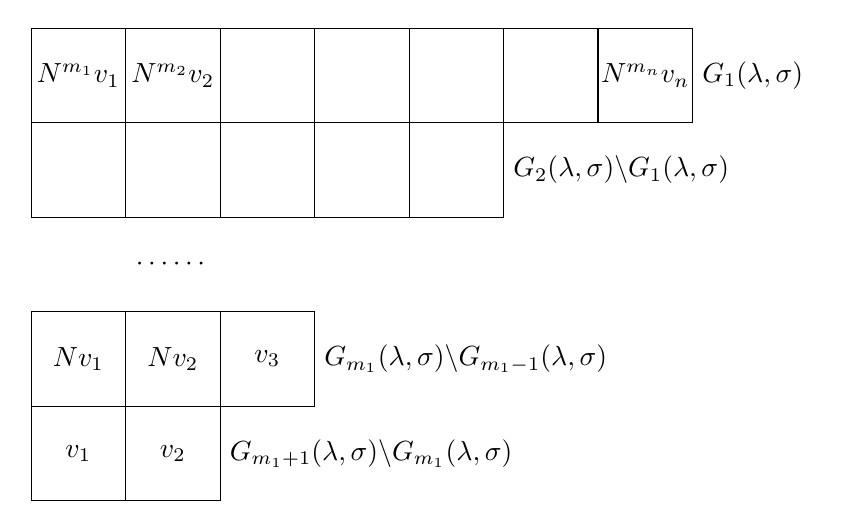
\begin{tikzpicture}[scale=1.2]
                  \foreach[count=\i] \len in {7, 7, 5, 3, 3, 2}
                      \draw (0, -\i+1) -- (\len, -\i+1);

                  \foreach \i in {0, 1, 2}
                      \draw (\i, -3) -- (\i, -5);

                  \draw (3, -3) -- (3, -4);

                  \foreach \i in {0,...,5}
                      \draw (\i, 0) -- (\i, -2);

                  \foreach \i in {6, 7}
                      \draw (\i, 0) -- (\i, -1);

                  \foreach \i in {1, 2} {
                      \node at (\i-.5, -4.5) {$v_{\i}$};
                      \node at (\i-.5, -.5) {$N^{m_{\i}}v_{\i}$};
                  }
                  \foreach \i in {1, 2}
                      \node at (\i-.5, -3.5) {$Nv_{\i}$};

                  \node at (3-.5, -3.5) {$v_{3}$};
                  \node at (6.5, -.5) {$N^{m_n}v_n$};
                  \node at (1.5, -2.5) {$\cdots\cdots$};

                  \node[anchor=west] at (7, -.5) {$G_1(\lambda,\sigma)$};
                  \node[anchor=west] at (5, -1.5) {$G_2(\lambda,\sigma) \backslash G_1(\lambda,\sigma)$};
                  \node[anchor=west] at (3, -3.5) {$G_{m_1}(\lambda,\sigma) \backslash G_{m_1-1}(\lambda,\sigma)$};
                  \node[anchor=west] at (2, -4.5) {$G_{m_1+1}(\lambda,\sigma) \backslash G_{m_1}(\lambda,\sigma)$};
              \end{tikzpicture}
              \caption{将若当基排列成Young图形式}
              \label{fig:17:若当基Young图形式}
          \end{figure}

    \item 接下来要确定每个若当循环基的长度,也就是Young图每一列的长度,我们应当从行的性质入手,因为这是我们目前仅有的可以计算的信息. 我们需要求解每个$G_j(\lambda,\sigma)$及其维数(目前只有维数有用,但后续求解具体若当基时其中的向量也是有用的),直到某个$G_j(\lambda,\sigma)$的维数等于$G_\lambda$的维数,因为Young图中所有方格与$G_\lambda$的一组基一一对应,因此方格总数就等于$G_\lambda$的维数. 另一方面由\autoref{thm:广义特征性质},$N$是$G_\lambda$上的幂零线性变换,且在其它广义特征子空间上是双射,因此在核空间最高次数也只能是$G_\lambda$的维数.

          在求出各个$G_j(\lambda,\sigma)$的维数后阶梯形状也即确定,因为各层向量个数确定了. 举个简单的例子,假设$G_\lambda$是11维空间,满足$G_1(\lambda,\sigma)$,$G_2(\lambda,\sigma)$,$G_3(\lambda,\sigma)$的维数分别为5,9,11. 对照Young图每行右侧的标注,这说明从最上方一行往下的向量个数依次为5,4($=9-5$),2($=11-9$),具体Young图为
          \begin{figure}[H]
              \centering
              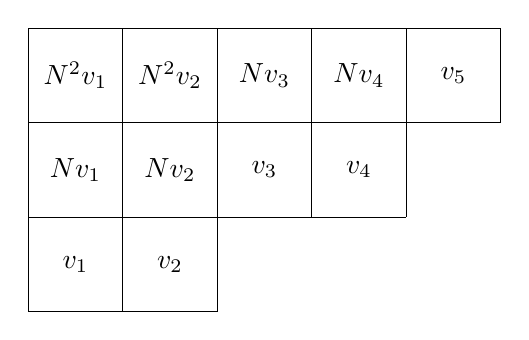
\begin{tikzpicture}[scale=1.2]
                  \foreach[count=\i] \len in {5, 5, 4, 2}
                      \draw (0, -\i+1) -- (\len, -\i+1);

                  \foreach \i in {0,...,5}
                      \draw (\i, 0) -- (\i, -1);
                  \foreach \i in {0,...,4}
                      \draw (\i, -1) -- (\i, -2);
                  \foreach \i in {0, 1, 2}
                      \draw (\i, -2) -- (\i, -3);

                  \node at (.5, -.5) {$N^2v_1$};
                  \node at (1.5, -.5) {$N^2v_2$};
                  \node at (2.5, -.5) {$Nv_3$};
                  \node at (3.5, -.5) {$Nv_4$};
                  \node at (4.5, -.5) {$v_5$};
                  \node at (.5, -1.5) {$Nv_1$};
                  \node at (1.5, -1.5) {$Nv_2$};
                  \node at (2.5, -1.5) {$v_3$};
                  \node at (3.5, -1.5) {$v_4$};
                  \node at (.5, -2.5) {$v_1$};
                  \node at (1.5, -2.5) {$v_2$};
              \end{tikzpicture}
          \end{figure}
          然后我们就能得到每组若当循环基的长度,即每个若当块的阶数,分别为$3,3,2,2,1$.
\end{enumerate}

基于上面的求解过程,我们就可以得到一般性的Young图大小的决定公式如下:
\begin{theorem}{}{Young图行长度}
    令$r_j$表示Young图从上至下第$j$行的格数,则有(其中$N=\sigma-\lambda I$):
    \begin{enumerate}
        \item $r_1=\dim V-r(N)$;
        \item $r_j=r(N)^{j-1}-r(N)^j(j>1)$.
    \end{enumerate}
\end{theorem}
\begin{proof}
    根据\autoref{fig:17:若当基Young图形式} 中每行右侧的标注的含义,第一行的格数就是$G_1(\lambda,\sigma)$的维数,即特征子空间的维数,即$\dim V-r(N)$;第$j(j>1)$行的格数就是$G_j(\lambda,\sigma)$的维数减去$G_{j-1}(\lambda,\sigma)$的维数,由线性映射基本定理,$\dim G_j(\lambda,\sigma)=\dim G_\lambda-r(N)^j$,$\dim G_{j-1}(\lambda,\sigma)=\dim G_\lambda-r(N)^{j-1}$,因此第$j$行的格数就是$r(N)^{j-1}-r(N)^j$.
\end{proof}

基于上述定理,我们可以进一步得到每个特征值对应的若当块个数和每个若当块大小的公式. 进一步地,这些公式实际上就表明了若当标准形的唯一性,因为每个特征值对应的若当块的个数和大小都可以被如下公式唯一确定. 我们将这一定理总结如下:
\begin{theorem}{}{若当标准形唯一}
    设$V$是$n$维复向量空间,$\sigma\in \mathcal{L}(V)$,$\lambda_1,\ldots,\lambda_m$为其互异的特征值,记$N_j=\sigma-\lambda_j I$,则主对角元为$\lambda_j$的若当块的个数$n_j$为
    \begin{equation} \label{eq:17:若当块个数}
        n_j=n-r(N_j),
    \end{equation}
    其中$t$级若当块$J_t(\lambda_j)$的个数$n_j(t)$为
    \begin{equation} \label{eq:17:若当块大小}
        n_j(t)=r(N_j^{t+1})+r(N_j^{t-1})-2r(N_j^t),
    \end{equation}
    以上公式表明,除若当块的排列次序外,一个线性变换对应的若当标准形唯一.
\end{theorem}
\begin{proof}
    实际上,证明这一定理就是要从\autoref{thm:Young图行长度} 中得到的Young图每行的长度推出Young图有多少列,以及每列的长度. 很显然,Young图的列数就是第一行的长度,即$\dim V-r(N_j)$. 进一步观察,我们知道Young图第$j$行与第$j+1$行的长度之差来源于有$r_j-r_{j+1}$(记号来源于\autoref{thm:Young图行长度})组循环若当基长度终止于$j$,因此大小为$j$的若当块的个数就是$r_j-r_{j+1}=r(N_j)^{t+1}+r(N_j)^{t-1}-2r(N_j)^t$.
\end{proof}

尽管我们理论上可以通过上述过程得到任意复向量空间上的线性变换的若当块的个数和大小,但我们知道,直接对线性变换计算特征值是困难的,因此更多的时候我们仍然是利用线性变换和它的矩阵表示的特征值与广义特征向量的对应关系,将求解线性变换的若当标准形转化为求解其某个矩阵表示的若当标准形.

于是我们讨论矩阵的情况. 我们考虑$P^{-1}AP=J$,其中$P$为过渡矩阵,$J$为$A$的若当标准形. 我们可以将$A$视为$\sigma(\alpha)=A\alpha$在自然基下的矩阵,于是$\sigma$在\autoref{cor:若当基存在} 给出的基(记为$B$)下的表示矩阵的求解方式就是$\sigma(B)=(B)J$,将$B$组成的矩阵记作$P$,代入$\sigma$的定义,$\sigma(B)=(B)J$就等同于$AP=PJ$,即$P^{-1}AP=J$,故如果我们要求矩阵相似于其若当标准形的过渡矩阵,问题转化为求解$\sigma(\alpha)=A\alpha$的若当基然后排列成矩阵即可.

然而我们知道,求解$\sigma$的若当基需要求解各个$G_i(\lambda,\sigma)=\ker(\sigma-\lambda I)^i$,代入$\sigma(\alpha)=A\alpha$可知,$G_i(\lambda,\sigma)$实际上就是$(A-\lambda I)^iX=0$的解. 所以对于矩阵而言,上述所有的过程都只是不断对矩阵求幂然后解线性方程组,因此是一定可解的. 我们用解空间替代各个$G_i(\lambda,\sigma)$重复上述过程可以得到如下定理:
\begin{theorem}{}{}
    设$A$是$n$阶复矩阵,$\lambda_1,\ldots,\lambda_m$为其互异的特征值,则主对角元为$\lambda_j$的若当块的个数$n_j$为
    \begin{equation} \label{eq:17:矩阵若当块个数}
        n_j=n-r(A-\lambda_j I),
    \end{equation}
    其中$t$级若当块$J_t(\lambda_j)$的个数$n_j(t)$为
    \begin{equation} \label{eq:17:矩阵若当块大小}
        n_j(t)=r(A-\lambda_j I)^{t+1}+r(A-\lambda_j I)^{t-1}-2r(A-\lambda_j I)^t,
    \end{equation}
    以上公式表明,除若当块的排列次序外,一个矩阵对应的若当标准形唯一.
\end{theorem}

最后我们需要提到一点,根据上面的叙述,若当标准形在不考虑若当块的排列顺序的情况下是唯一的. 因此任一复数域上矩阵均有唯一的若当标准形(相似标准形),因此我们可以知道,两矩阵相似的一个充要条件是两矩阵有相同的若当标准形(不考虑若当块的排列顺序),这也是判定两个矩阵是否相似的关键,当然之后我们还会学到其它判定方式,届时我们再做总结.

接下来我们将讨论如何求出Young图中所有方格中的向量,当然实际上只需确定每个终止向量即可得到所有向量. 在正式讨论之前,我们先考虑一种投机取巧的方式. 事实上,如果题目只要求我们求解矩阵的若当标准形时,如果我们要求解过渡矩阵,也有简单的方法. 要求$P$使得$P^{-1}AP=J$,则有$AP=PJ$. 假定$P$为$n$阶矩阵,我们可以设$P=(X_1,\ldots,X_n)$,剩下的任务就是解方程了. 因此这种方法非常简单,缺陷在于绕开了若当基这一本质的问题.
\begin{example}{}{}
    利用上述方法求解矩阵\[\begin{pmatrix}
            2 & 3 & 2 \\ 1 & 8 & 2 \\ -2 & -14 & -3
        \end{pmatrix}\]的若当标准形以及对应的过渡矩阵.
\end{example}

\begin{solution}

\end{solution}

下面我们将讨论对于一般的线性变换,无法投机取巧时,或者希望从更本质的角度求解时,我们应当使用的方法.

\begin{center}
    \textbf{\heiti 第二步\quad 求解 $\boldsymbol{v_1,\ldots,v_n}$}
\end{center}

\begin{enumerate}
    \item 实际上,我们在前述求解若当块大小的过程中求出了各个$G_j(\lambda,\sigma)$,接下来我们需要利用这些向量将之前确定形状的阶梯内容填满. 我们首先将阶梯最上方的向量确定,实际上就是利用求出的$G_{m_1+1}(\lambda,\sigma)$(也就是$V$)和$G_{m_1}(\lambda,\sigma)$求出二者之差. 似乎很简单,但若仔细思索便会发现线性空间的差并不一定好求. 举一个简单的例子,设$G_{m_1+1}(\lambda,\sigma)=\{\alpha_1,\alpha_2,\alpha_3,\alpha_4\}$,$G_{m_1}(\lambda,\sigma)=\{\beta_1,\beta_2\}$. 这其中出现的所有向量可能都完全不一样,所以作差并不容易. 但我们有一种好方法,如果我们每次从$G_{m_1+1}(\lambda,\sigma)$中挑选两个向量和$G_{m_1}(\lambda,\sigma)$中的两个向量放在一起,如果这四个向量线性无关,这就说明这两个挑出的向量就是作差的结果. 原因在于这相当于$G_{m_1}(\lambda,\sigma)$直和这两个向量长成的空间后得到了$G_{m_1+1}(\lambda,\sigma)$. 如果四个向量线性相关,这说明挑选的向量有在$G_{m_1}(\lambda,\sigma)$中的.

    \item 接下来继续计算第二行中的向量. 实际上算出第一行后第二行中部分向量就已经确定了,例如图上的$Nv_1$和$Nv_2$. 我们这时用类似的方法求解$G_{m_1}(\lambda,\sigma)$和$G_{m_1-1}(\lambda,\sigma)$的差,如图只需要确定一个向量,但这一个向量的确定除了要像(a)中一样每次从$G_{m_1}(\lambda,\sigma)$中选择一个与$G_{m_1-1}(\lambda,\sigma)$的基一起判断线性相关性外,还需要确保这个向量和已经求出的$Nv_1$和$Nv_2$是线性无关的,因为它们构成$G_{m_1}(\lambda,\sigma)$的一组基.

          总结一下,处于$G_j(\lambda,\sigma)\backslash G_{j-1}(\lambda,\sigma)$对应的行的需要补充的向量$v$应当满足如下三个条件:
          \begin{enumerate}
              \item $v\in G_j(\lambda,\sigma)$;

              \item $v\notin G_{j-1}(\lambda,\sigma)$(通过加入$G_{j-1}(\lambda,\sigma)$)的基保证线性无关判断);

              \item $v$与同一行中左边已求出的向量线性无关.
          \end{enumerate}

    \item 最后,我们将所有求出的基按照若当基原先的排列顺序重新组合即可. 如果求矩阵相似于若当标准形的过渡矩阵,则按顺序按列摆放即可.
\end{enumerate}

我们可以通过一个例子来说明上述过程.
\begin{example}{}{}
    设$V$是由两个变量$x,y$生成的次数不大于2的多项式函数(例如$xy^2$不是,因为次数等于1+2=3,$x^2+y$是)关于一般的多项式加法和数乘构成的线性空间,于是我们可以取一组基为$\{1,x,y,x^2,y^2,xy\}$,定义$\sigma\in \mathcal{L}(V)$为
    \[\sigma(f(x,y))=\dfrac{\partial}{\partial x}f(x,y).\]
    求$V$的一组基使得$\sigma$在这组基下的矩阵是若当标准形.
\end{example}
\begin{solution}

\end{solution}

\section{若当标准形的应用}
\subsection{求解不变子空间}
在不变子空间一节中我们提到,我们可以利用若当标准形求解不变子空间. 下面是一个与若当块直接相关的例子:
\begin{example}{}{}
    设$V$为$n$维复向量空间,$\sigma\in \mathcal{L}(V)$,$\sigma$在基$v_1,\ldots,v_n$下的矩阵是一个若当块
    \[\begin{pmatrix}
            \lambda & 1       & 0      & \cdots & 0       \\
            0       & \lambda & 1      & \cdots & 0       \\
            \vdots  & \vdots  & \vdots & \ddots & \vdots  \\
            0       & 0       & 0      & \cdots & \lambda
        \end{pmatrix},\]
    证明:
    \begin{enumerate}
        \item $V$中包含$v_n$的不变子空间只有$V$自身;

        \item $V$中任意非零不变子空间都包含$v_1$;

        \item $V$不能分解为两个非平凡的不变子空间的直和;

        \item $V$中有且仅有$n+1$个不变子空间,它们分别是
              \[\{0\},\spa(v_1),\spa(v_1,v_2),\ldots,\spa(v_1,\ldots,v_{n-1},v_n)\]
    \end{enumerate}
\end{example}

\begin{solution}
    \begin{enumerate}
        \item 设$W$是包含$v_n$的不变子空间,根据线性映射矩阵表示的定义,$\sigma(v_n)=\lambda v_n+v_{n-1}\in W$,故$v_{n-1}\in W$,同理可得$v_{n-2},\ldots,v_1\in W$,即$W=V$.

        \item 设$U$为任一非零不变子空间,那么$U$中存在一个非零向量$v$,则$v$一定可以表达为
              \[v=k_1v_1+\cdots+k_sv_s(s\leqslant n),\]
              其中$k_s\neq 0$. 由$\sigma(v)\in U$以及线性映射矩阵表示有
              \begin{align*}
                  \sigma(v) & = \lambda k_1v_1+k_2(\lambda v_2+v_1)+\cdots+k_s(\lambda v_s+v_{s-1}) \\
                            & = \lambda v+k_2v_1+\cdots+k_sv_{s-1}\in U,
              \end{align*}
              因此$k_2v_1+\cdots+k_sv_{s-1}\in U$,同理进一步作用$\sigma$有$k_3v_1+\cdots+k_sv_{s-2}\in U$,以此类推有$k_sv_1\in U$. 又$k_s\neq 0$,故$v_1\in U$,命题得证.

        \item 利用上一点显然.

        \item 显然$\{0\},\spa(v_1),\spa(v_1,v_2),\ldots,\spa(v_1,\ldots,v_{n-1},v_n)$都是不变子空间,下面证明不变子空间一定在它们当中.

              设$U$为任一不变子空间,若$U=\{0\}$,则也符合结论. 我们考虑非零的情况,设$\beta_1,\ldots,\beta_s$是$U$的一组基,并且假设
              \[\beta_i=a_{i1}v_1+a_{i2}v_2+\cdots+a_{it}v_t,\enspace i=1,2,\ldots,s\]
              其中满足至少有一个$i$使得$a_{it}\neq 0$(把所有基下表示末尾的0去除即可). 对于满足$a_{it}\neq 0$的$i$,由于$U$是不变子空间,故$\sigma(\beta_i)\in U$,与第二点证明完全相同,我们得到
              \begin{align*}
                  a_{i2}v_1+a_{i3}v_2+\cdots+a_{it}v_{t-1}\in U, \\
                  a_{i3}v_1+a_{i4}v_2+\cdots+a_{it}v_{t-2}\in U, \\
                  \cdots                                         \\
                  a_{i,t-1}v_1+a_{it}v_2\in U,                   \\
                  a_{it}v_1\in U.
              \end{align*}
              由于$a_{it}\neq 0$,故由最后的式子知道$v_1\in U$. 代入倒数第二个式子知道$v_2\in U$,以此类推,最终得到$\spa(v_1,\ldots,v_t)\subset U$,而$U\subset\spa(v_1,\ldots,v_t)$显然(因为每个$\beta_i$都在其中),故命题得证.
    \end{enumerate}
\end{solution}

因此我们如果能将线性变换在一组基下表示为若当块,我们就可以很快地利用这一例子的结论写出其不变子空间. 但我们有时候会遇到线性变换在一组基下表示为多个若当块的情况,这时我们可能需要通过组合不同若当块对应的不变子空间来得到线性变换的不变子空间(很容易知道不相交的不变子空间的直和还是不变子空间,因为矩阵表示还是分块对角矩阵),并且同时还要证明组合出来的就是全部的不变子空间. 下面就是一个非常经典的例子:
\begin{example}{}{}
    设$V$是复数域上的$n$维线性空间,$\sigma\in\mathcal{L}(V)$,若$\sigma$有$n$个不同的特征值$\lambda_1,\ldots,\lambda_n$,求$\sigma$的不变子空间的个数.
\end{example}
\begin{solution}
    显然$\sigma$可对角化,每个对角元素就是一阶若当块,因此我们需要考虑组合这些若当块对应的基构成新的不变子空间. 由可对角化我们有
    \[V=V_{\lambda_1}\oplus\cdots\oplus V_{\lambda_n},\]
    结合$\dim V=n$可知每个特征子空间都是1维的. 根据我们组合的思想,我们知道对于任意的$1\leqslant j_1<j_2<\cdots<j_r\leqslant n$,$r=1,2,\ldots,n$,$V_{\lambda_{j_1}}\oplus\cdots\oplus V_{\lambda_{j_r}}$都是不变子空间. 这样的不变子空间加上零空间的个数总和为$\mathrm{C}_n^0+\mathrm{C}_n^1+\cdots+\mathrm{C}_n^n=2^n$.

    下面我们需要说明这些不变子空间是全部的不变子空间. 设$U$为任一不变子空间,若为零空间则符合要求,若不是零空间,设$\dim U=m>0$,$U$的一组基为$\beta_1,\ldots,\beta_m$,将其扩充为$V$的一组基$\beta_1,\ldots,\beta_m,\beta_{m+1},\ldots,\beta_n$,则在这组基下$\sigma$的矩阵为
    \[B=\begin{pmatrix}
            A & C \\ O & D
        \end{pmatrix},\]
    于是$\sigma\vert_W$的矩阵为$A$,对应特征多项式$|\lambda E-A|$可以整除$\sigma$的特征多项式$|\lambda E-B|=|\lambda E-A||\lambda E-D|$,由于$\sigma$有$n$个不同的特征值,因此$\sigma\vert_W$必定有$m$个不同的特征值$\lambda_{l_1},\ldots,\lambda_{l_m}$,且$1\leqslant l_1<\cdots<l_m\leqslant n$,而对每个特征值$\lambda_{l_i}$都有特征向量$\alpha_i\in W$,满足$\sigma\vert_W(\alpha_i)=\lambda_{l_i}\alpha_i$,因此$\sigma(\alpha)=\lambda_{l_i}\alpha_i$,即$\alpha_i\in V_{\lambda_{l_i}}$,故$V_{\lambda_{l_1}}\oplus\cdots\oplus V_{\lambda_{l_m}}\subset U$. 再结合
    \[\dim(V_{\lambda_{l_1}}\oplus\cdots\oplus V_{\lambda_{l_m}})=m=\dim U,\]
    故$U=V_{\lambda_{l_1}}\oplus\cdots\oplus V_{\lambda_{l_m}}$,故所有不变子空间都是之前讨论的$2^n$种之一,命题得证.
\end{solution}

当然需要注意的是,不变子空间的个数不一定有限,例如对于数乘变换$\sigma=kI\in\mathcal{L}(V)$,很容易验证$V$的任意子空间都是其不变子空间.

\subsection{矩阵求幂与马尔可夫链}

若当标准形的另一个应用在于我们可以利用它计算矩阵的幂,因为若当块的幂的计算是简单的,这一点与对角矩阵是类似的:
\[J_k(a)^n=(aE+J_k(0))^n=a^nE+\mathrm{C}_n^1a^{n-1}J_k(0)+\cdots+\mathrm{C}_n^nJ_k(0)^n\]
同时我们也知道$J_k(0)^k=O$(幂零矩阵),所以利用若当标准形求解矩阵的幂是简单的. 我们来看一个例子:
\begin{example}{}{}
    设$A=\begin{pmatrix}
            2 & 6 & -15 \\ 1 & 1 & -5 \\ 1 & 2 & -6
        \end{pmatrix}$,求$A^{m}(m\geqslant 1)$.
\end{example}
\begin{solution}

\end{solution}

下面是一个非常经典的例子,在接下来的讨论中还会有应用:
\begin{example}{}{若当m次幂}
    设$J=J_n(a)$是特征值为$a$的$n$阶若当块,求$J^m$的若当标准形,其中$m$为非零整数.
\end{example}
\begin{solution}
    我们需要分别考虑$a\neq 0$和$a=0$的情况:
    \begin{enumerate}
        \item 当$a\neq 0$时,首先显然$J^m$的特征值都为$a^m$,我们先处理$m\geqslant 1$的情况,我们有
              \[J^m=(aE+J(0))^m=a^mE+\mathrm{C}_m^1a^{m-1}J_n(0)+\cdots+\mathrm{C}_m^mJ_n(0)^m.\]
              故$r(J^m-a^mE_n)=r(\mathrm{C}_m^1a^{m-1}J_n(0)+\cdots+\mathrm{C}_m^mJ_n(0)^m)=n-1$(很容易通过$J_n(0)$的幂次的特点写出这一矩阵,然后通过行列式秩判断),因此根据\autoref{thm:若当标准形唯一} 可知$J^m$的若当块个数为$n-(n-1)=1$,因此$J^m$的若当标准形就是$J_n(a^m)$.

              然后我们考虑$m=-1$的情况,显然$J^{-1}$的特征值为$a^{-1}$,这里我们借用\autoref{ex:分式求逆1} 的分式思想,得到
              \[J^{-1}=\dfrac{1}{a}E_n-\dfrac{1}{a^2}J_n(0)+\cdots+(-1)^{n-1}\dfrac{1}{a^n}J_n(0)^{n-1}.\]
              故$r(J^{-1}-\dfrac{1}{a}E_n)=r(-\dfrac{1}{a^2}J_n(0)+\cdots+(-1)^{n-1}\dfrac{1}{a^n}J_n(0)^{n-1})=n-1$,因此$J^{-1}$的若当块个数为$n-(n-1)=1$,因此$J^{-1}$的若当标准形就是$J_n(a^{-1})$.

              最后处理$m\leqslant -2$的情况,注意到$J^m=(J_n^{-1})^{-m}$,故根据前面$m\geqslant 1$的讨论,$J^m$的若当标准形就是$J_n((a^{-1})^{-m})=J_n(a^m)$.

              综上所述,无论$m$取什么整数值,$J^m$的若当标准形就是$J_n(a^m)$.

        \item 当$a=0$时,我们有$m\geqslant n$时$J^m=O$,此时若当标准形也就是零矩阵. 我们考虑$m<n$的情况,我们需要使用\autoref{thm:若当标准形唯一} 的结论来辅助我们求解$J^m$的若当标准形,因此我们需要研究$(J^m)^k$的秩. 我们做带余除法,$n=mq+r(0\leqslant r<m)$,则根据$J_n(0)$的幂次的特点,我们有
              \[r((J^m)^k)=n-mk,\enspace 0\leqslant k\leqslant q,\enspace r((J^m)^k)=0,\enspace k\geqslant q+1.\]
              因此
              \begin{enumerate}
                  \item $1\leqslant k<q$时,$J_k(0)$的个数为$r((J^m)^{k-1})+r((J^m)^{k+1})-2r((J^m)^k)=(n-m(k-1))+(n-m(k+1))-2(n-mk)=0$;
                  \item $k=q$时,$J_k(0)$的个数为$r((J^m)^{q-1})+r((J^m)^{q+1})-2r((J^m)^q)=(n-m(q-1))+0-2(n-mq)=m-r$;
                  \item $k=q+1$时,$J_k(0)$的个数为$r((J^m)^q)+r((J^m)^{q+2})-2r((J^m)^{q+1})=(n-mq)+0-0=r$.
                  \item $k>q+1$时,$J_k(0)$的个数为0.
              \end{enumerate}
              综上所述,$J^m$的若当标准形是$\diag(J_q(0),\ldots,J_q(0),J_{q+1}(0),\ldots,J_{q+1}(0))$,其中$J_q(0)$的个数为$m-r$,$J_{q+1}(0)$的个数为$r$.
    \end{enumerate}
\end{solution}

由于复数域上任意矩阵都有若当标准形,因此利用若当标准形,我们可以求出复数域上任意矩阵的任意幂次. 于是我们会有一个问题,即任意给定一个矩阵,当我们取其幂次趋向于无穷时,会得到一个什么样的矩阵呢?是所有元素都有限的矩阵,还是有些元素可能趋于无穷了呢?

\subsection{若当标准形与矩阵分解}
矩阵分解是我们讨论标准形时绕不开的话题,接下来我们讨论若当标准形应用于矩阵分解的情形. 我们首先讨论平方根分解,这一点是之前线性变换平方根讨论的延续. 下面这一结论是相当经典的:
\begin{theorem}{}{若当标准形m次根}
    在复数域上,我们有如下关于若当标准形的根式结论:
    \begin{enumerate}
        \item 设$a\neq 0$,则存在矩阵$A$使得$A^m=J_n(a)$;
        \item 当$n\geqslant 2$时,不存在矩阵$A$使得$A^m=J_n(0)$.
    \end{enumerate}
\end{theorem}

\begin{proof}
    \begin{enumerate}
        \item 根据\autoref{ex:若当m次幂},我们知道$J_n(a)^m\sim J_n(a^m)$. 设$b^m=a$(在复数域上一定存在这样的$b$),则$J_n(b)^m\sim J_n(a)$,因此存在可逆矩阵$P$使得$P^{-1}J_n(b)^mP=J_n(a)$,取$A=P^{-1}J_n(b)P$即可.

        \item 反证法. 若存在矩阵$A$使得$A^m=J_n(0)$,则$A$显然也为$n$阶幂零矩阵,因此有$A^n=O$(因此至少有$m\leqslant n$). 设$n=mq-r(m\geqslant 2,0\leqslant r<m)$,则$O=A^{n+r}=(A^m)^q=J_n(0)^q\neq O$,这是因为$J_n(0)$至少需要$n$次才能化零,但$n=mq-r(m\geqslant 2,0\leqslant r<m)$表明$q<n$,故矛盾.
    \end{enumerate}
\end{proof}

接下来我们考虑之前已经证明的\autoref{thm:幂零平方根} 的\ref*{item:16:幂零平方根:2},即可逆线性变换一定有平方根,我们现在可以使用若当标准形的方式证明. 我们直接使用矩阵证明即可,因为基固定的情况下矩阵和线性映射一一对应. 因为可逆线性变换对应可逆矩阵$A$,可逆矩阵特征值均不为0,因此每个对应的若当标准形$J$的若当块对角线上都不为0,均有平方根(即上述定理中$m=2$,我们记$B^2=J$). 进一步地,由于一定存在可逆矩阵$P$使得$P^{-1}AP=J$,我们取$C=PBP^{-1}$,则$C^2=PB^2P^{-1}=PJP^{-1}=A$,故我们找到了任意可逆矩阵对应的平方根$C$. 这一结论显然可以进一步推广,即任意复数域上的可逆线性变换和可逆矩阵一定有$m$次方根.

利用若当标准形,我们还可以有以下著名的Jordan-Chevalley分解. 这一定理的证明过程将会给出我们利用若当标准形证明一般矩阵性质的通用方法,一般包含如下步骤:
\begin{enumerate}
    \item 证明结论对于若当块成立;
    \item 证明结论对于若当标准形成立;
    \item 利用问题在相似下的不变性证明结论对于一般矩阵成立.
\end{enumerate}

事实上,上面讨论任意复可逆矩阵均有平方根也是遵循这一范式证明的,我们也是先证明了对角线元素非零的若当块一定有平方根,那么自然若当标准形是由若当块构成的分块对角矩阵也满足这一性质,然后利用$(P^{-1}AP)^n=P^{-1}A^nP$这一相似具有的运算特点证明对一般可逆矩阵有平方根成立. 总而言之,当我们希望使用若当标准形证明矩阵具有的性质时,这些性质在相似下要有一定的不变性,然后我们遵照上述范式即可给出证明. 因此,我们发现了研究相似标准形的一个重要的意义,因为这些很简单的矩阵一般而言都是具有很好的性质的,再结合很多性质在相似下都可以保持,因此我们可以通过研究更容易处理的相似标准形来研究一般矩阵的性质. 下面我们就开始证明这一著名的分解:

\begin{theorem}{Jordan-Chevalley分解}{}
    设$A$是$n$阶复矩阵,则$A$可分解为$A=B+C$,其中$B,C$满足如下条件:
    \begin{enumerate}
        \item $B$是可对角化的;
        \item $C$是幂零的;
        \item $BC=CB$;
        \item $B,C$均可以表示为$A$的多项式.
    \end{enumerate}
    不仅如此,满足上述条件1-3的分解是唯一的.
\end{theorem}

\begin{proof}
    我们首先对若当块$J_n(a)$证明这一定理. 事实上这非常显然,我们取$B=aE_n$,$C=J_n(0)$,则$B$可对角化,$C$是幂零的,且$BC=CB=aJ_n(0)$. 又因为$O=C^n=(J_n(a)-B)^n$,因此我们取$f(x)=(x-a)^n+a$,代入$x=J_n(a)$有
    $f(J_n(a))=(J_n(a)-aE_n)^n+aE_n=aE_n=B$,因此$B$表示为了$A$的多项式,而$C=J_n(a)-B=J_n(a)-f(J_n(a))$也是$A$的多项式.

    接下来推广到若当标准形$J$,我们假设$J$互不相同的特征值为$\lambda_1,\ldots,\lambda_m$,设每个特征值$\lambda_i$对应$s_i$个若当块,则可以将$J$表示为
    \[J=\begin{pmatrix}
            J_{11} &        &          &        &        &        &          \\
                   & \ddots &          &        &        &        &          \\
                   &        & J_{1s_1} &        &        &        &          \\
                   &        &          & \ddots &        &        &          \\
                   &        &          &        & J_{m1} &        &          \\
                   &        &          &        &        & \ddots &          \\
                   &        &          &        &        &        & J_{ms_m}
        \end{pmatrix}.\]
    对每个若当块$J_{ij}$,假设若当块大小为$k_{ij}$,我们类似于前面对若当块的讨论取出每个$M_{ij}=\lambda_i E_{k_{ij}}$,$N_{ij}=J_{k_{ij}}(0)$,然后将这些矩阵按$J$的顺序排列成分块对角矩阵即可得到$M$和$N$,则$J=M+N$,$M$可对角化,$N$是幂零的,且$MN=NM$是容易验证的.

    我们设每个特征值$\lambda_i$对应的最大的若当块的阶数为$k_i$,因此$(J_{ij}-\lambda_{ij})^{k_i}=O$. 我们知道$(\lambda-\lambda_1)^{k_1},\ldots,(\lambda-\lambda_m)^{k_m}$是两两互素的多项式,因此由\nameref{thm:中国剩余定理}可知,存在多项式$f(\lambda)$满足
    \[f(\lambda)=g_i(\lambda)(\lambda-\lambda_i)^{k_i}+\lambda_i,\enspace i=1,\ldots,m\]
    故$f(J_{ij})=g_i(J_{ij})(J_{ij}-\lambda_i)^{k_i}+\lambda_iE_{k_{ij}}=\lambda_iE_{k_{ij}}=M_{ij}$,因此$f(J)=M$也成立. 同理$N=J-M=J-f(J)$也是$J$的多项式,因此命题结论对若当标准形都成立.

    接下来考虑一般情形,设$P^{-1}AP=J$,则$A=PJP^{-1}=P(M+N)P^{-1}=PMP^{-1}+PNP^{-1}$. 取$B=PMP^{-1}$,$C=PNP^{-1}$,则$B$可对角化,$C$是幂零的,且$BC=CB$,$B,C$均可以表示为$A$的多项式都可以从$M,N$具有这样的性质立刻得到,即这一问题是在相似下不变的.

    最后证明唯一性. 假设$A$有另一满足1-3的分解$A=B'+C'$,则$B-B'=C'-C$,由$B'C'=C'B'$,结合$A=B'+C'$可知$AB'=B'A,AC'=C'A$,又因为$B=f(A)$,故$BB'=B'B$,同理有$CC'=C'C$. 设$C^r=O,C'^t=O$,用二项式定理可知$(C-C')^{r+t}=O$,因此$(B-B')^{r+t}=O$.

    我们知道$B$和$B'$可对角化且$BB'=B'B$,根据上一讲的习题可知它们可以同时对角化,即存在可逆矩阵$Q$使得$Q^{-1}BQ$和$Q^{-1}B'Q$均为对角矩阵. 注意到
    \[(Q^{-1}BQ-Q^{-1}B'Q)^{r+t}=(Q^{-1}(B-B')Q)^{r+t}=Q^{-1}(B-B')^{r+t}Q=O,\]
    又两对角矩阵的差是对角矩阵,因此只能有$Q^{-1}BQ=Q^{-1}B'Q$,即$B=B'$,从而$C=C'$也成立,因此唯一性得证.
\end{proof}

\subsection{求解微分方程}

取一常系数微分方程如下:
\[\dfrac{\mathrm{d}f_1}{\mathrm{d}x^2}-a\dfrac{\mathrm{d}f_1}{\mathrm{d}x}=bf_1.\]
令$\dfrac{\mathrm{d}f_1}{\mathrm{d}x}=f_2$,则上式可以改写为
\[\begin{cases}
        \dfrac{\mathrm{d}f_1}{\mathrm{d}x}=f_2, \\
        \dfrac{\mathrm{d}f_2}{\mathrm{d}x}=af_2+bf_1.
    \end{cases}\]
我们可以将上述方程写成矩阵形式:
\[\dfrac{\mathrm{d}}{\mathrm{d}x}\begin{pmatrix}
        f_1 \\ f_2
    \end{pmatrix}=\begin{pmatrix}
        0 & 1 \\ b & a
    \end{pmatrix}\begin{pmatrix}
        f_1 \\ f_2
    \end{pmatrix}.\]

类似地,$n$阶常微分方程
\[\dfrac{\mathrm{d}f_1}{\mathrm{d}x^n}-a_{n-1}\dfrac{\mathrm{d}f_1}{\mathrm{d}x^{n-1}}-\cdots-a_1\dfrac{\mathrm{d}f_1}{\mathrm{d}x}=bf_1\]
可以改写为
\[\dfrac{\mathrm{d}}{\mathrm{d}x}\begin{pmatrix}
        f_1 \\ f_2 \\ \vdots \\ f_n
    \end{pmatrix}=\begin{pmatrix}
        0      & 1      & 0      & \cdots & 0       \\
        0      & 0      & 1      & \cdots & 0       \\
        \vdots & \vdots & \vdots & \ddots & \vdots  \\
        0      & 0      & 0      & \cdots & 1       \\
        b      & a_1    & a_2    & \cdots & a_{n-1}
    \end{pmatrix}\begin{pmatrix}
        f_1 \\ f_2 \\ \vdots \\ f_n
    \end{pmatrix}=C\begin{pmatrix}
        f_1 \\ f_2 \\ \vdots \\ f_n
    \end{pmatrix}.\]
若有$P^{-1}CP=J$,令
\[P^{-1}\begin{pmatrix}
        f_1 \\ f_2 \\ \vdots \\ f_n
    \end{pmatrix}=\begin{pmatrix}
        g_1 \\ g_2 \\ \vdots \\ g_n
    \end{pmatrix},\]
于是我们有
\[\dfrac{\mathrm{d}}{\mathrm{d}x}\begin{pmatrix}
        g_1 \\ g_2 \\ \vdots \\ g_n
    \end{pmatrix}=J\begin{pmatrix}
        g_1 \\ g_2 \\ \vdots \\ g_n
    \end{pmatrix}.\]

一个直观的事情是$J$越简单方程越容易解,因此这时若当标准形就能帮助我们解决这一问题.

\subsection{求解线性递推方程}

数列的线性递推方程求解是我们高中就曾经接触过的问题,在行列式的运算技巧中我们也曾提及二阶齐次线性递推方程的求解,不过那种方法显然缺乏普适性. 很自然地,我们希望能寻求某种方法来解决$m$阶线性递推方程,不过在此之前,我们需要明确这其中蕴含的线性性究竟在何处.

让我们先从二阶开始,考虑$a_n = k_1 a_{n - 1} + k_2 a_{n - 2}$,显然其特征方程为$x^2 - k_1 x - k_2 = 0$,考虑无重根($\Delta = k_1 + 4k_2 \neq 0$)的情况,有$\lambda_1 = \dfrac{k_1 + \sqrt{k_1 + 4k_2}}{2}, \lambda_2 = \dfrac{k_1 - \sqrt{k_1 + 4k_2}}{2}$,且通项为$a_n = A \lambda_1^n + B \lambda_2^n$,其中$A, B$为待定常数. 而事实上,这个递推方程可以用一个线性映射去表示. 设$T \in \mathcal{L}(\mathbf{F}^2)$为$T(x_1, x_2) = (x_2, k_2 x_1 + k_1 x_2)$,则有$T(a_{n - 2}, a_{n - 1}) = (a_{n - 1}, a_n)$,便可以得到$T^n(a_0, a_1) = (a_n, a_{n + 1})$,也就是说,如果对初值进行$n$次线性变换,我们便可以得到第$n$项的值,但这个计算量过于庞大了. 而回忆我们先前处理算子的幂的方法,很快便能回想起相似标准型,所以接下来我们需要转向求出这一算子的特征值与特征向量.

考虑$T(x_1, x_2) = \lambda (x_1, x_2)$,得到方程组$\begin{cases} x_2 = \lambda x_1 \\ k_2 x_1 + k_1 x_2 = \lambda x_2 \end{cases}.$ 考虑到特征向量不为零向量,所以消去$x_1, x_2$后可以得到关于$\lambda$的方程$\lambda^2 - k_1 \lambda - k_2 = 0$,所以这个方程才会被称为特征方程,因为它的根是算子的特征值. 在没有重根的情况下,解得两个特征值为$\lambda_1, \lambda_2$,而对应的特征向量为$v_1 = (1, \lambda_1), v_2 = (1, \lambda_2)$. 我们知道对应不同特征值的特征向量是线性无关的,并且这里的数量正好等于空间维数,所以这两个特征向量构成了空间的一组基,且算子在这组基下的矩阵表示是简单的,为对角阵$\Lambda = \begin{pmatrix} \lambda_1 & 0 \\ 0 & \lambda_2 \end{pmatrix}$. 设$(a_0, a_1) = c_1 v_1 + c_2 v_2$,而使用矩阵求出坐标再代入基是计算量较小的,所以有 $\Lambda^n \begin{pmatrix}
        c_1 \\ c_2
    \end{pmatrix} = \begin{pmatrix}
        c_1 \lambda_1^n \\ c_2 \lambda_2^n
    \end{pmatrix}$,这便是$(a_n, a_{n + 1})$在这组基下的坐标,代入$v_1, v_2$即可得到通解$a_n = c_1 \lambda_1^n + c_2 \lambda_2^n$.

而对于$m$阶线性递推方程$a_n = k_1 a_{n - 1} + k_2 a_{n - 2} + \cdots + k_m a_{n - m}$,其无重根的情况是二阶的简单推广. 考虑$T \in \mathcal{L}(F^m)$,$T(x_1, x_2, \cdots, x_m) = (x_2, x_3, \cdots, k_m x_1 + k_{m - 1} x_2 + \cdots + k_1 x_m)$,则$T(a_{n - m}, a_{n - m + 1}, \cdots, a_{n - 1}) = (a_{n - m + 1}, a_{n - m + 2}, \cdots, a_n)$,对应的特征方程为$x^m - k_1 x^{m - 1} - \cdots - k_m = 0$,得到特征值为$\lambda_1, \lambda_2, \cdots, \lambda_m$,而对应的特征向量为$v_i = (1, \lambda_i, \lambda_i^2, \cdots, \lambda_i^{m - 1})$,通解为$a_n = \sum_{i = 1}^m c_i \lambda_i^n$. 另一个有趣的事实是所有的特征向量也能组成一个 Vandermonde 矩阵,这也可以从另一个侧面印证为什么要求没有重根.

那么如果存在重根又会发生什么情况呢?我们依然先以一个二阶线性递推方程为例,考虑$a_n = 2 \lambda_0 a_{n - 1} - \lambda_0^2 a_{n - 2}$,构造相应的算子$T(x_1, x_2) = (x_2, 2 \lambda_0 x_2 - \lambda_0^2 x_1)$,则$T(a_{n - 2}, a_{n - 1}) = (a_{n - 1}, a_n)$,特征值易求得为$\lambda_0$,对应特征向量为$(1, \lambda_0)$. 特征空间为一维的,显然不能够对角化,所以它应该对应为二阶的若当块的情况,已知$v_1 = (1, \lambda_0)$,求出满足$(T - \lambda_0 I)v_2 = v_1$的$v_2$即求出了若当基. 满足条件的一个$v_2 = (0, 1)$,在这组基下$T$的矩阵表示为$\begin{pmatrix} \lambda_0 & 1 \\ 0 & \lambda_0 \end{pmatrix} = \lambda_0 I + J$,其中$J = \begin{pmatrix} 0 & 1 \\ 0 & 0 \end{pmatrix}$ 且 $J^2 = O$. 设$(a_0, a_1) = c_1v_1 + c_2v_2$,那么有
\begin{align*}
    M^n \begin{pmatrix} c_1 \\ c_2 \end{pmatrix} & = (\lambda_0 I + J)^n \begin{pmatrix} c_1 \\ c_2 \end{pmatrix} \\
    & = (\lambda^n I + n \lambda^{n - 1} J) \begin{pmatrix} c_1 \\ c_2 \end{pmatrix} \\
    & = \begin{pmatrix} \lambda^n & n \lambda^{n - 1} \\ 0 & \lambda^n \end{pmatrix} \begin{pmatrix} c_1 \\ c_2 \end{pmatrix} \\
    & = \begin{pmatrix} c_1 \lambda^n + n c_2 \lambda^{n - 1} \\ d \lambda^n \end{pmatrix}.
\end{align*}
从而代入$v_1, v_2$有$a_n = c_1 \lambda_0^n + n c_2 \lambda_0^{n - 1}$.

进而我们可以考虑一个$m$阶线性递推方程,且其特征方程有$m$重根$\lambda_0 \neq 0$的情况(特征值为$0$是退化的),这时对应的是一个$m$阶的若当块,重点在于求出其对应的若当基. 首先对应的算子$T$的形式应当为$T(x_1, x_2, \cdots, x_m) = (x_2, x_3, \cdots, (-1)^{m + 1} \binom{m}{0} \lambda_0^m x_1 + (-1)^m \binom{m}{1} \lambda_0^{m - 1} x_2 + \cdots + (-1)^2 \binom{m}{m - 1} \lambda_0 x_{m})$,要求出特征向量即求出满足$(T - \lambda_0 I)v_1 = 0$的$v_1$,这一线性方程组的系数矩阵如下:\[
    \begin{pmatrix}
        -\lambda_0 & 1 & 0 & \cdots & 0 \\
        0 & -\lambda_0 & 1 & \cdots & 0 \\
        \vdots & \vdots & \vdots & \ddots & \vdots \\
        0 & 0 & 0 & \cdots & 1 \\
        (-1)^{m + 1} \binom{m}{0} \lambda_0^m & (-1)^m \binom{m}{1} \lambda_0^{m - 1} & (-1)^{m - 1} \binom{m}{2} \lambda_0^{m - 2} & \cdots & ((-1)^2 \binom{m}{m - 1} - 1) \lambda_0
    \end{pmatrix}
\]
我们能轻松得到$v_1 = (\lambda_0^0, \lambda_0, \lambda_0^2, \cdots, \lambda_0^{m - 1})$是满足前$m-1$行的,代入验证也满足第$m$行. 因为前$m-1$行是线性无关的,所以我们基本上可以宣称第$m$行是前$m-1$行的线性组合,也就是说这个矩阵的秩为$m-1$. 但是,这个线性组合的系数在后续求解若当基的过程中相当重要,所以我们还是要求出来. 记以上系数矩阵为$\begin{pmatrix}
    \beta_1 \\ \beta_2 \\ \vdots \\ \beta_m
\end{pmatrix}$,$\beta_i$均是行向量. 这个系数求解的关键在于第$2$到第$m-1$个坐标都是有两个行向量来控制的,并且$\beta_m$每个是以组合数为基础的,我们能够很自然的联想到杨辉三角. 首先第$1$个坐标能够给出第一个系数$t_1 = (-1)^m \binom{m - 1}{0} \lambda_0^{m - 1}$,然后第$2$个坐标结合杨辉三角便可以得到$t_2 = (-1)^{m - 1} \binom{m - 1}{1} \lambda_0^{m - 2}$,以此类推,直到第$m-1$个坐标$t_{i - 1} = (-1)^2 \binom{m-1}{m-2} \lambda_0$. 第$m$个坐标我们需要验证其正确性,因为其减去了$1$所以形式上有所区别,但我们可以将其改写为$((-1)^2 \binom{m}{m - 1} - \binom{m - 1}{m - 1}) \lambda_0 = ((-1)^2 \binom{m - 1}{m - 2}) \lambda_0$,与$t_{i-1}$一致. 所以我们有 \[
    \beta_m = t_1 \beta_1 + t_2 \beta_2 + \cdots + t_{m - 1} \beta_{m - 1}.
\]
其中$t_i = (-1)^{m + 1 - i} \binom{m - 1}{i - 1} \lambda_0^{m - i}$.

因为$v_1$的求解是基于齐次线性方程组,所以系数的作用不是很明确. 但当我们开始求解$v_2, v_3, \ldots, v_m$时,这就意味着我们需要处理非齐次线性方程组,需要验证$v_1, v_2, \ldots, v_{m-1}$的第$m$个坐标能根据前$m-1$个坐标由系数$t_i$组合得到. 以$v_2$为例,我们需要验证$\lambda_0^{m-1} = \sum_{i = 1}^{m-1} t_i \lambda_0^{i-1} = \sum_{i = 1}^{m-1} (-1)^{m + 1 - i} \binom{m - 1}{i - 1} \lambda_0^{m - 1}$. 我们可以将其化简为 \begin{align*}
    \sum_{i = 1}^{m-1} (-1)^{m + 1 - i} \binom{m - 1}{i - 1} & = 1 \\
    \sum_{i = 0}^{m-1} \binom{m-1}{i} (-1)^{m - i} & = 0.
\end{align*}
这是二项式定理的一个特殊情况,所以这个等式是成立的. 根据前$m-1$行,我们可以得到$v_2 = (0, 1, 2 \lambda_0, 3 \lambda_0^2, \ldots, (m - 1) \lambda_0^{m - 2})$. 以此类推,仅依据前$m-1$行的计算,我们可以得到$v_j = (0, 0, \ldots, \binom{j - 1}{j - 1} \lambda_0^0, \binom{j}{j - 1} \lambda_0^1, \ldots, \binom{m - 1}{j - 1} \lambda_0^{m - j})$,且第$1$个非零坐标为第$j$个. 接下来便需要验证$v_j, 1 \leqslant j \leqslant m - 1$的第$m$个坐标能由前$m-1$个坐标线性组合得到,即 \[
    \binom{m - 1}{j - 1} \lambda_0^{m - j} = \sum_{i = 1}^{m - 1} t_i \binom{i - 1}{j - 1} \lambda_0^{i - 1}.
\]
代入后化简得到需要证明的组合恒等式 \[
    \sum_{i = j}^m (-1)^{m + 1 - i} \binom{m - 1}{i - 1} \binom{i - 1}{j - 1} = 0.
\]

\begin{proof}
    注意到 \begin{align*}
        \binom{m - 1}{i - 1} \binom{i - 1}{j - 1} & = \dfrac{(m - 1)!}{(i - 1)! (m - i)!} \dfrac{(i - 1)!}{(j - 1)! (i - j)!} \\ & = \dfrac{(m - 1)!}{(j - 1)! (m - j)!} \dfrac{(m - j)!}{(i - j)! (m - i)!} \\ & = \binom{m - 1}{j - 1} \binom{m - j}{i - j},
    \end{align*}
    所以 \begin{align*}
        \sum_{i = j}^m (-1)^{m + 1 - i} \binom{m - 1}{i - 1} \binom{i - 1}{j - 1} & = \sum_{i = j}^m (-1)^{m + 1 - i} \binom{m - 1}{j - 1} \binom{m - j}{i - j} \\
        & = \binom{m - 1}{j - 1} \sum_{t = 0}^k (-1)^(k + i - t  + 1 - i) \binom{k}{t} \\
        & = \binom{m - 1}{j - 1} \sum_{t = 0}^k \binom{k}{t} (-1)^{k + 1 - t} \\
        & = \binom{m - 1}{j - 1} (-1) (1 - 1)^k = 0.
    \end{align*}
    其中 $t = i - j, k = m - j$.
\end{proof}

由上可知$v_j$的求解是正确的,这样我们便得到了对应的若当基,$T$在这组基下的表示矩阵为$\lambda_0 I + J$. 设初值在若当基下的表示系数为$c_1, c_2, \ldots, c_m$,则有 \begin{align*}
    M^n \begin{pmatrix}
        c_1 \\ c_2 \\ \vdots \\ c_m
    \end{pmatrix}
    & = (\lambda_0 I + J)^n \begin{pmatrix}
        c_1 \\ c_2 \\ \vdots \\ c_m
    \end{pmatrix} \\ & = (\lambda_0^n I + n \lambda_0^{n - 1} J + \cdots + \binom{n}{m - 1} \lambda_0^{n - m + 1} J^{m - 1}) \begin{pmatrix}
        c_1 \\ c_2 \\ \vdots \\ c_m
    \end{pmatrix} \\
    & = \begin{pmatrix}
        \lambda_0^n & n \lambda_0^{n - 1} & \cdots & \binom{n}{m - 1} \lambda_0^{n - m + 1} \\
        0 & \lambda_0^n & \cdots & \binom{n}{m - 2} \lambda_0^{n - m + 2} \\
        \vdots & \vdots & \ddots & \vdots \\
        0 & 0 & \cdots & \lambda_0^n
    \end{pmatrix} \begin{pmatrix}
        c_1 \\ c_2 \\ \vdots \\ c_m
    \end{pmatrix} \\ & = \begin{pmatrix}
        c_1 \lambda_0^n + n c_2 \lambda_0^{n - 1} + \cdots + \binom{n}{m - 1} c_m \lambda_0^{n - m + 1} \\
        c_2 \lambda_0^n + n c_3 \lambda_0^{n - 1} + \cdots + \binom{n}{m - 2} c_m \lambda_0^{n - m + 2} \\
        \vdots \\
        c_m \lambda_0^n
    \end{pmatrix}.
\end{align*}

代入$\{v_j\}$即可得到通解
\[
    a_n = \sum_{i = 1}^m c_i \binom{n}{i - 1} \lambda_0^{n - i + 1}.
\]

而对于一般的若当标准型来说,只需要求出相应的基,然后利用分块对角矩阵的幂次运算即可得到坐标,代入基即可求得通解. 不过需要注意的是,对于$m$阶若当标准型下$n$阶的若当块,其对应的若当基是我们在$m$重根中讨论的前$n$个向量,即
    \begin{align*}
        v_1 & = (1, \lambda_0, \lambda_0^2, \ldots, \lambda_0^{m - 1}), \\ v_2 & = (0, 1, 2 \lambda_0, \ldots, (n - 1) \lambda_0^{m - 2}), \\ & \ldots \\ v_n & = (0, 0, \ldots, \binom{n - 1}{n - 1} \lambda_0^0, \binom{n}{n - 1} \lambda_0^1, \ldots, \binom{m - 1}{n - 1} \lambda_0^{m - n}),
    \end{align*}
    而非前$n$个坐标.

下面给出一道例题,请读者自行尝试.

\begin{example}{}{}
    求解线性递推方程$a_n = 5a_{n - 1} - 8a_{n - 2} + 4a_{n - 3}$,其中$a_0 = 2, a_1 = 4, a_2 = 9$.
\end{example}

\section{实数域上的若当标准形} \label{sec:实数域上的若当标准形}

\begin{theorem}{}{相似域不变性}
    设$A,B$为域$\mathbf{F}$上的同阶方阵,域$\mathbf{K}$是域$\mathbf{F}$的一个扩域,则$A,B$在域$\mathbf{K}$上相似当且仅当它们在域$\mathbf{F}$上也相似.
\end{theorem}
\begin{proof}

\end{proof}

\begin{theorem}{}{实数域上的若当标准形}
    设$A$是$n$阶实矩阵,则$A$在实数域上相似于如下分块对角矩阵:
    \begin{enumerate}
        \item $J=\diag(J_{r_1}(\lambda_1),\ldots,J_{r_k}(\lambda_k),J_{s_1}(a_1,b_1),J_{s_l}(a_l,b_l))$;
        \item $\tilde{J}=\diag(J_{r_1}(\lambda_1),\ldots,J_{r_k}(\lambda_k),\tilde{J}_{s_1}(a_1,b_1),\tilde{J}_{s_l}(a_l,b_l))$
    \end{enumerate}
    其中$\lambda_1,\ldots,\lambda_k,a_1,b_1,\ldots,a_l,b_l$都是实数,$b_1,\ldots,b_l$都非零,$J_{r_i}(\lambda_i)$表示以$\lambda_i$为特征值的通常意义下的若当块,$R_j=\begin{pmatrix}
            a_j & b_j \\ -b_j & a_j
        \end{pmatrix},C_2=\begin{pmatrix}
            0 & 0 \\ 1 & 0
        \end{pmatrix}$,
    \[J_{s_i}(a_i,b_i)=\begin{pmatrix}
            R_i & I_2 &        &        &     \\
                & R_i & I_2    &        &     \\
                &     & \ddots & \ddots &     \\
                &     &        & R_i    & I_2 \\
                &     &        &        & R_i
        \end{pmatrix},\enspace \tilde{J}_{s_i}(a_i,b_i)=\begin{pmatrix}
            R_i & C_2 &        &        &     \\
                & R_i & C_2    &        &     \\
                &     & \ddots & \ddots &     \\
                &     &        & R_i    & C_2 \\
                &     &        &        & R_i
        \end{pmatrix}.\]
\end{theorem}
\begin{proof}

\end{proof}

\vspace{2ex}
\centerline{\heiti \Large 内容总结}

\vspace{2ex}
\centerline{\heiti \Large 习题}

\vspace{2ex}
{\kaishu }
\begin{flushright}
    \kaishu

\end{flushright}

\centerline{\heiti A组}
\begin{enumerate}
    \item
\end{enumerate}

\centerline{\heiti B组}
\begin{enumerate}
    \item 求矩阵\[\begin{pmatrix}
                  2 & 3 & 0  & -1 & 2 & -2 \\ -1 & 0 & 2 & 1 & -1 & -2 \\
                  1 & 3 & 2  & 0  & 1 & -4 \\ 5 & 6 & -1 & -2 & 5 & -3 \\
                  3 & 3 & -1 & -2 & 3 & -1 \\ 1 & 3 & 2 & 0 & 1 & -4
              \end{pmatrix}\]的若当标准形以及相应的过渡矩阵(提示:这一矩阵是幂零指数为3的幂零矩阵).

    \item 设$A=\begin{pmatrix}
                  2 & 1 & 1 \\ -2 & -1 & -2 \\ 1 & 1 & 2
              \end{pmatrix}$,求$A$的若当标准形$J$和矩阵$P$,使得$P^{-1}AP=J$.

    \item 定义$\sigma\in \mathcal{L}(\mathbf{C}^3)$为$\sigma(z_1,z_2,z_3)=(z_2,z_3,0)$. 证明不存在$\tau\in \mathcal{L}(\mathbf{C}^3)$使得$\tau^2=\sigma$.

    \item 证明:存在复数域上的对称矩阵$B,C$,使得$A=BC$,并且可以指定$B,C$中任意一个可逆.

    \item 斐波那契序列(Fibonacci sequence)$\{F_n\}$满足如下定义:
          \[
              F_0 = 0, F_1 = 1, F_n = F_{n - 2} + F_{n - 1}, n \geqslant 2.
          \]
          定义$T \in \mathcal{L}(\mathbf{R}^2)$为$T(x_1, x_2) = (x_2, x_1 + x_2)$.
          \begin{enumerate}
            \item 证明:对于任意非负整数$n$,$T^n(0, 1) = (F_n, F_{n + 1})$.
            \item 求$T$的特征值和对应的特征向量.
            \item 求$F_n$的通项公式.
            \item 证明:对于任意非负整数$n$,$F_n$是最接近$\dfrac{\varphi^n}{\sqrt{5}}$的整数,其中$\varphi = \dfrac{1 + \sqrt{5}}{2}$.
          \end{enumerate}
\end{enumerate}

\centerline{\heiti C组}
\begin{enumerate}
    \item
\end{enumerate}

\phantomsection
\section*{19 多项式的进一步讨论}
\addcontentsline{toc}{section}{19 多项式的进一步讨论}

\vspace{2ex}

\centerline{\heiti A组}
\begin{enumerate}
    \item
\end{enumerate}

\centerline{\heiti B组}
\begin{enumerate}
    \item
\end{enumerate}

\centerline{\heiti C组}
\begin{enumerate}
    \item
\end{enumerate}

\clearpage

\phantomsection
\section*{20 有理标准形}
\addcontentsline{toc}{section}{20 有理标准形}

\vspace{2ex}

\centerline{\heiti A组}
\begin{enumerate}
    \item
\end{enumerate}

\centerline{\heiti B组}
\begin{enumerate}
    \item
\end{enumerate}

\centerline{\heiti C组}
\begin{enumerate}
    \item
\end{enumerate}

\clearpage

\LUchapter{对称多项式和Young图}

\chapter{内积空间}

\section{内积和范数}

\subsection{内积和范数的定义及性质}

前面研究的所有空间都是线性空间,只注重于线性结构,忽视了向量的度量性质,如向量的长度、夹角等. 但度量性质恰是在分析、几何问题中不可缺少的. 故从此章起,我们引入度量的概念,将线性空间推广为内积空间.

\term{内积}\index{neiji@内积 (inner product)}的引入始于我们曾在高中研究过的 $\mathbf{R}^{2}$ 与 $\mathbf{R}^{3}$ 上的向量点积,范数则是始于向量的长度概念. 内积即是点积性质的推广,本质上就是一个函数,它把 $ V $ 中元素的每个有序对 $(u, v)$ 都映射成一个数$ \langle u, v \rangle \in \mathbf{F}$,并且具有以下性质:

\begin{enumerate}
    \item 正定性:$\forall v \in V, \enspace \langle v, v \rangle \geqslant 0, \enspace \langle v, v \rangle = 0 \iff v = \vec{0}$;

    \item 第一个位置的加性:$\forall u, v, w \in V, \enspace \langle u + v, w \rangle = \langle u, w \rangle + \langle v, w \rangle$;

    \item 第一个位置的齐性:$\forall \lambda \in \mathbf{F}, \enspace \forall u, v \in V, \enspace \langle \lambda u, v \rangle = \lambda \langle u, v \rangle$;

    \item 共轭对称性:$\forall u, v \in V, \enspace \langle u, v \rangle = \overline{\langle v, u \rangle}$.
\end{enumerate}

每个实数都等于它的复共轭,所以在处理实向量空间时,共轭对称性实际上转变为对称性,即:$\forall u, v \in V, \enspace \langle u, v \rangle = \langle v, u \rangle$.

而由以上定义,我们可以快速得到以下性质:

\begin{enumerate}
    \item 对于每个取定的 $u \in V$,将 $ v $ 变为 $\langle v, u \rangle$ 的函数是 $ V $ 到 $\mathbf{F}$ 的线性映射.

    \item $\forall u \in V, \enspace \langle \vec{0}, u \rangle = \langle u, \vec{0} \rangle = 0$.

    \item $\forall u, v, w \in V, \enspace \langle u, v + w \rangle = \langle u, v \rangle + \langle u, w \rangle$.

    \item $\forall \lambda \in \mathbf{F}, \enspace \forall u, v \in V, \enspace \langle u, \lambda v \rangle = \overline{\lambda} \langle u, v \rangle$.
\end{enumerate}

其实从以上的定义与性质可以发现,实内积空间上的内积与我们之后要提到的双线性函数有着密不可分的联系——实线性空间上的正定对称双线性函数实际上就是该空间上的一个内积,在此先按下不表.

内积定义完成后,便可由该内积确定一个相应的范数:对于 $v \in V$,$v$ 的\term{范数}\index{fanshu@范数 (norm)}(记作 $ \lVert v \rVert $)定义为 $ \lVert v \rVert = \sqrt{\langle v, v \rangle}$. 并且具有以下性质:

\begin{enumerate}
    \item $\forall v \in V, \enspace \left\lVert v \right\rVert = 0 \iff v = \vec{0}$.

    \item $\forall v \in V, \enspace \forall \lambda \in \mathbf{F}, \enspace \left\lVert \lambda v \right\rVert  = \left\lvert \lambda \right\rvert \lVert v \rVert$.
\end{enumerate}

上述性质留给读者自证,从中我们也能发现一个普遍原理:处理范数的平方通常比直接处理范数更容易.

以下给出几个内积和范数的示例:

\begin{example} \label{ex:23:内积和范数}
    \begin{enumerate}
        \item $\mathbf{F}^{n}$ 上的欧几里得内积定义为:
              \[\left\langle (w_1, \ldots, w_n), (z_1, \ldots, z_n)\right\rangle = w_1\overline{z_1} + \cdots + w_n\overline{z_n} = \vec{w}\overline{\vec{z}}^{\mathrm{T}}\]
              对应范数:
              \[\left\lVert (z_1, \ldots, z_n) \right\rVert  = \sqrt{\lvert z^2_1 \rvert + \cdots + \lvert z^2_n \rvert}\]

        \item \label{item:23:内积和范数:2}
              定义在 $ \left[-1, 1\right] $ 上的连续实值函数构成的向量空间可定义内积如下:
              \[\left\langle f, g\right\rangle = \int_{-1}^1f(x)g(x)\,\mathrm{d}x\]
              对应范数:
              \[\left\lVert f \right\rVert = \sqrt{\int_{-1}^1(f(x))^2\,\mathrm{d}x}\]
    \end{enumerate}
\end{example}

\subsection{正交的定义 \quad 基于正交的性质}

以下给出一个关键定义:

\begin{definition} \index{zhengjiao@正交 (orthogonal)}
    两个向量 $u, v \in V$ 称为\term{正交的},如果 $\langle u, v\rangle = 0$.
\end{definition}

该定义中向量的次序是无关紧要的,因为 $\langle u, v\rangle = 0 \iff \langle v, u\rangle = 0$.

那么正交的定义关键在何处呢?以下给出 $\mathbf{R}^{n}$ 空间上夹角的定义以供理解(证明良定义需要用到 Cauchy-Schwarz 不等式):

\begin{definition}
    设 $u, v \in \mathbf{R}^{n}$,则 $u, v$ 的夹角 $ \theta $ 为$ \theta = \arccos \dfrac{\langle u, v\rangle}{\lVert u \rVert \lVert v \rVert}$.
\end{definition}

那么我们可以发现,当两向量正交时,它们的夹角就是 $\dfrac{\pi}{2}$,也就是我们在几何中常说的垂直,它能将我们导向一些重要的定理.

让我们从一些简单的结果开始研究正交性,比如正交性与 $ \vec{0} $ 的关系:

\begin{enumerate}
    \item $ \vec{0} $ 正交与 $V$ 中的任意向量.

    \item $ \vec{0} $ 是 $V$ 中唯一一个与自身正交的向量.
\end{enumerate}

然后是熟悉的勾股定理在内积空间上的推广:

\begin{theorem}
    设 $u, v$ 是 $V$ 中的正交向量,则 $\lVert u + v \rVert^2 = \lVert u \rVert^2 + \lVert v \rVert^2 $.
\end{theorem}

注意勾股定理的逆定理仅在实内积空间上成立.

借助于正交的性质,我们能够简化很多与内积相关的计算,进而会很自然的思考这样一个问题:一个向量能否分解两个互相正交的向量?

从而便引进了正交分解:

\begin{theorem}
    设 $u, v \in V$ 且 $v \neq \vec{0}$. 令 $ c = \dfrac{\langle u, v\rangle}{\lVert v \rVert^2}, \enspace w = u - \dfrac{\langle u, v\rangle}{\lVert v \rVert^2}v$. 则 $\langle w, v\rangle = 0$且 $u = cv + w$.
\end{theorem}

而通过正交分解,我们可以证明一个数学中最重要的不等式(之一):\term{Cauchy-Schwarz 不等式}.

\begin{theorem}[Cauchy-Schwarz 不等式] \index{Cauchy@Cauchy-Schwarz 不等式 (Cauchy-Schwarz inequality)}
    设 $u, v \in V$. 则 $\left\lvert \left\langle u, v\right\rangle \right\rvert \leqslant \lVert u \rVert\lVert v \rVert$. 等号成立当且仅当 $u, v$ 之一是另一个的标量倍.
\end{theorem}

也可以通过引入参数,利用二次三项式的判别式证明.

借助 Cauchy-Schwarz 不等式,我们可以得到三角不等式:

\begin{theorem}
    设 $u, v \in V$. 则 $\lVert u, v \rVert \leqslant \lVert u \rVert + \lVert v \rVert$. 等号成立当且仅当 $u, v$ 之一是另一个的非负标量倍.
\end{theorem}

其几何解释就是俗称的三角形两边之和小于第三边.

另一个与几何相关的结论就是平行四边形恒等式:

\begin{theorem}
    设 $u, v \in V$. 则 $ \lVert u + v \rVert^{2} + \lVert u - v \rVert^{2} = 2(\lVert u \rVert^{2} + \lVert v \rVert^{2})$.
\end{theorem}

其几何解释为任意的平行四边形两对角线的长度的平方和等于四边长度的平方和.

以下为另外几个与内积有关的恒等式,我们会在证明正规算子和自伴算子的性质时运用到它们:

\begin{example}
    证明下列式子成立:
    \begin{enumerate}
        \item $\mathbf{F} = \mathbf{R}$ 时:
              \begin{gather}
                  \label{eq:23:内积和范数的性质1}
                  \langle u, v\rangle = \frac{1}{4}\left( \lVert u + v \rVert^2 - \lVert u - v \rVert^2\right) \\
                  \label{eq:23:内积和范数的性质2}
                  \langle Tu, v\rangle + \langle Tv, u\rangle = \frac{1}{2}\left(\langle T(u + v), u + v\rangle - \langle T(u - v), u - v\rangle\right)
              \end{gather}

        \item $\mathbf{F} = \mathbf{C}$ 时:
              \begin{gather}
                  \label{eq:23:内积和范数的性质3}
                  \langle u, v\rangle = \frac{1}{4}\left((\lVert u + v \rVert^2 - \lVert u - v \rVert^2) + \i(\lVert u + \i v \rVert^2 - \lVert u - \i v \rVert^2)\right) \\
                  \label{eq:23:内积和范数的性质4}
                  \begin{aligned}
                      \langle Tu, v\rangle ={} & \frac{1}{4}  ((\langle T(u + v), u + v\rangle - \langle T(u - v), u - v\rangle)     \\
                                               & + \i(\langle T(u + \i v), u + \i v\rangle + \langle T(u - \i v), u - \i v\rangle)).
                  \end{aligned}
              \end{gather}
    \end{enumerate}

\end{example}

\section{标准正交基}

这一节我们将沿着正交的路径接着往下走,看看如果整个向量组乃至一组基都是单位化的且互相正交的话,会有怎样的性质. 我们也会讲解如何获取这样一组基的算法,并介绍 Riesz 表示定理,其揭示了线性泛函和内积的深刻联系.

\begin{definition} \index{zhengjiao!biaozhun@标准正交 (orthonormal), 规范正交}
    如果一个向量组的每个向量范数都是 1 且与其他向量正交则称这个向量组是\term{标准正交}(规范正交)的.
\end{definition}

在本书的剩余部分中我们都称此性质为标准正交.

由以上定义,我们得出:$ V $ 上的向量组 $ e_1, \ldots , e_n $ 是标准正交的,如果
\[ \langle e_j, e_k \rangle = \delta _{jk} = \begin{cases}
        1 & j = k    \\
        0 & j \neq k
    \end{cases} \]

标准正交组的优势在于处理其线性组合的范数很方便.

\begin{theorem}
    若 $e_1, \ldots , e_m$ 是 $ V $ 中的标准正交向量组,则对 $\forall a_1, \ldots, a_m \in \mathbf{F}$ 均有
    \[ \lVert a_1e_1 + \cdots + a_ne_n\rVert^2 = \lvert a_1 \rvert^2 + \cdots + \lvert a_n \rvert^2.\]
\end{theorem}

反复使用勾股定理即可证明. 该定理也有一个重要推论:

\begin{theorem}
    任何标准正交向量组都是线性无关的.
\end{theorem}

令其线性组合为 $ \vec{0} $ 即证.

\begin{example} \label{ex:22:标准正交组}
    设 $e_1, \ldots , e_m$ 是 $ V $ 的标准正交组. 设 $ v \in V $. 证明
    \[ \lVert v \rVert^2 = \lvert \langle v, e_1\rangle \rvert^2 + \cdots + \lvert \langle v, e_m\rangle \rvert^2 \]
    当且仅当 $ v \in \spa(e_1, \ldots , e_m)$.
\end{example}

既然标准正交组都是线性无关的,很自然我们就会想到在线性空间中最有用的线性无关组:基. 也就有了标准正交基的定义.

\begin{definition}
    $ V $ 的标准正交基是 $ V $ 中的标准正交向量组构成的基.
\end{definition}

而由向量组确定为基的等价条件,易知长度为 $\dim V$ 的标准正交向量组都是$ V $ 的标准正交基.

标准正交基的优势就在于表出向量的表出系数可以提前确定.

\begin{theorem}
    设 $e_1, \ldots e_n$ 是 $ V $ 标准正交基且 $ v \in V$. 则
    \begin{equation} \label{eq:23:Fourier展开}
        v = \langle v, e_1 \rangle e_1 + \cdots + \langle v, e_n \rangle e_n
    \end{equation}
    且
    \[ \lVert v \rVert^2 = \lvert \langle v, e_1\rangle \rvert^2 + \cdots + \lvert \langle v, e_m\rangle \rvert^2. \]
\end{theorem}

此为\autoref{ex:22:标准正交组} 的特例. \autoref{eq:23:Fourier展开} 也被称为 $ v $ 的 Fourier 展开,其中每个系数 $ \langle v, e_j \rangle $ 被称为 $ v $ 的 Fourier 系数.

标准正交基的性质十分美妙,但我们取出一组基使得其恰好是标准正交基是十分困难的,所幸前人已经研究出了一套算法,可以将所有线性无关组转变为标准正交组,且张成空间相同.

\begin{theorem}[Gram-Schmidt 过程] \index{Gram@Gram-Schmidt 过程 (Gram-Schmidt process)}
    设 $v_1, \ldots ,v_n$ 是 $ V $ 中的线性无关向量组. 设 $e_1 = \dfrac{v_1}{\lVert v_1 \rVert}$. 对于 $ j = 2, \ldots , m$,定义 $ e_j $ 如下:
    \[ e_j = \frac{v_j - \langle v_j, e_1 \rangle e_1 - \cdots - \langle v_j, e_{j - 1} \rangle e_{j - 1} }{\lVert v_j - \langle v_j, e_1 \rangle e_1 - \cdots - \langle v_j, e_{j - 1} \rangle e_{j - 1} \rVert}\]
    则 $e_1, \ldots , e_m $ 是 $ V $ 中的标准正交组,使得对 $ j = 1, \ldots , m $ 有
    \[ \spa(v_1, \ldots, v_j) = \spa(e_1, \ldots, e_j) \]
\end{theorem}

证明前半部分使用归纳法,后半部分证明两向量组等价即可.

让我们简单运用一下 Gram-Schmidt 过程.
\begin{example}
    求 $\mathbf{R}[x]_2$ 的一组标准正交基,内积定义为 $\langle p, q \rangle = \displaystyle\int_{-1}^1 p(x)q(x)\,\mathrm{d}x$.
\end{example}

不难发现,Gram-Schmidt 过程实际上可以分成两部分:
\begin{enumerate}
    \item 正交化:定义 $ u_1 = v_1 , \enspace u_j = v_j - \langle v_j, e_1 \rangle e_1 - \cdots - \langle v_j, e_{j - 1} \rangle e_{j - 1}, \enspace j = 2, \ldots , m$,此时 $u_1, \ldots , u_m$ 已经互相正交.

    \item 单位化:$ e_j = \dfrac{u_j}{\lVert u_j \rVert} , \enspace j = 1, \ldots , m$,从而有 $\lVert e_j \rVert = 1, \enspace j = 1, \ldots , m$
\end{enumerate}

Gram-Schmidt 过程可以说是线性代数计算较为困难的方面之一,也是应试经常考察的方面,需要多加注意.

借助 Gram-Schmidt 过程,显然我们可以得到以下结论:
\begin{enumerate}
    \item 每个有限维内积空间都有标准正交基;

    \item 设 $ V $ 是有限的. 则 $ V $ 中每个标准正交向量组都可以扩充成 $ V $ 的标准正交基.
\end{enumerate}
也可以得到这样一个定理.

\begin{theorem}[Schur 定理] \label{thm:23:Schur} \index{Schur@Schur 定理 (Schur's triangularization theorem)}
    设 $ V $ 是有限维的复内积空间,且 $ T \in \mathcal{L}(V) $,则 $ T $ 关于 $ V $ 的某个标准正交基具有上三角矩阵.
\end{theorem}

证明并不复杂,只需要结合\autoref{thm:20:上三角矩阵存在} 和 Gram-Schmidt 过程即可. 虽然十分浅显,但它迈出了我们在内积空间上算子简化表示的第一步,在更进一步的结论中我们会运用到它.

在此我们先打住,回忆一下内积的定义,其本质上就是一个函数,它把 $ V $ 中元素的每个有序对 $(u, v)$ 都映射成一个数$ \langle u, v \rangle \in \mathbf{F}$,而我们也很熟悉一类把 $ V $ 中元素映射成一个数的函数,即所谓的线性泛函. 那么这两者之间是否存在着某种联系?我们先借助几个例子观察一下.

\begin{example}
    \begin{enumerate}
        \item 定义如下的函数 $\varphi : \mathbf{F}^{3} \rightarrow \mathbf{F}$
              \[\varphi(z_1, z_2, z_3) = 2z_1 - 5z_2 + z_3\]
              是 $\mathbf{F}^{3}$ 上的线性泛函. 我们可以将其写成以下形式:$ \forall z \in \mathbf{F}^{3}$,
              \[\varphi(z) = \langle z, u\rangle\]
              其中 $u = (2, -5, 1)$.

        \item 定义如下的函数 $\varphi$: $\mathbf{R}[x]_2 \rightarrow \mathbf{R}$
              \[\varphi(p) = \int_{-1}^1 p(t)(\cos(\pi t))\,\mathrm{d}t\]
              是 $\mathbf{R}[x]_2$ 上的线性泛函, 此处的内积为\autoref{ex:23:内积和范数} \ref*{item:23:内积和范数:2} 中定义的. 但以下的事实并不那么显然:$ \exists u \in \mathbf{R}[x]_2$, 使得$\forall p \in \mathbf{R}[x]_2$ 均有 $ \varphi (p) = \langle p, u\rangle $.
    \end{enumerate}
\end{example}

可以发现,若是固定内积的第二个位置上的向量,内积就等同于一个线性泛函. 即对于确定的 $ u \in V , \enspace \varphi(v) = \langle v, u \rangle$ 就是一个线性泛函. 下面的定理揭示了这两者的关系,其指出 $ V $ 上所有的线性泛函都是这种形式:
\begin{theorem}[Riesz 表示定理] \label{thm:23:Riesz} \index{Riesz@Riesz 表示定理 (Riesz representation theorem)}
    设 $ V $ 是有限维的且 $ \varphi $ 是 $ V $ 上的线性泛函,则存在唯一的向量$u \in V$ 使得对 $\forall v \in V$ 均有 $ \varphi(v) = \langle v, u\rangle $.
\end{theorem}

\begin{proof}
    存在性:设 $e_1, \ldots , e_n$ 是 $ V $ 上的一组标准正交基,则对 $\forall v \in V $ 均有
    \begin{align*}
        \varphi (v) & = \varphi(\langle v, e_1 \rangle e_1 + \cdots + \langle v, e_n \rangle e_n )           \\
                    & = \langle v, e_1 \rangle \varphi (e_1) + \cdots + \langle v, e_n \rangle \varphi (e_n) \\
                    & = \langle v, \overline{\varphi(e_1)}e_1 + \cdots + \overline{\varphi(e_n)}e_n \rangle
    \end{align*}
    故取
    \[ u = \overline{\varphi(e_1)}e_1 + \cdots + \overline{\varphi(e_n)}e_n, \]
    对 $\forall v \in V$ 都有 $\varphi(v) = \langle v, u \rangle $.

    唯一性:设 $ u_1, u_2 \in V $ 使得对 $\forall v \in V $ 均有
    \[\varphi(v) = \langle v, u_1 \rangle = \langle v, u_2 \rangle.\]
    则对 $\forall v \in V $ 均有
    \[ 0 = \langle v, u_1 \rangle - \langle v, u_2 \rangle = \langle v, u_1 - u_2 \rangle\]
    取 $ v = u_1 - u_2 $ 可得 $ u_1 - u_2 = 0 $,即 $ u_1 = u_2 $,唯一性得证.
\end{proof}

Riesz 表示定理不仅证明了内积和线性泛函的联系,也给出了求解向量 $ u $ 的公式使其满足$ \forall v \in V $,使得 $ \varphi(v) = \langle v, u\rangle $. 具体来说,就是
\[ u = \overline{\varphi(e_1)}e_1 + \cdots + \overline{\varphi(e_n)}e_n, \]
而根据 Riesz 表示定理,我们知道 $ u $ 只依赖于线性泛函 $ \varphi $,所以选取任意一组$ V $ 上的标准正交基都会计算出相同的结果.

按以往的经验,该节的内容常在考试中作为大题单独考察.
\begin{example}
    定义在 $ V = \mathbf{R}^3 $ 上的运算
    \[ \langle \vec{x}, \vec{y} \rangle_V = x_1 y_1 + x_2 y_2 + (x_2 + x_3)(y_2 + y_3) \]
    其中 $ \vec{x} = (x_1, x_2, x_3),\enspace \vec{y} = (y_1, y_2, y_3) $.
    \begin{enumerate}
        \item 验证 $ \langle \cdot, \cdot \rangle_V $ 是 $ \mathbf{R}^3 $ 上的一个内积;

        \item 求 $ \mathbf{R}^3 $ 在 $ \langle \cdot, \cdot \rangle_V $ 下的一组标准正交基;

        \item 求 $ \vec{\beta} \in V $ 使得 $ \forall \vec{x} \in V,\enspace x_1 + 2x_2 = \langle \vec{x}, \vec{\beta} \rangle_V $.
    \end{enumerate}
\end{example}

\section{正交补}

本节的内容更偏向于几何方向,将带领大家了解空间的正交补,以及一种特殊的映射:正交投影. 并介绍一下极小化问题及一点应用.

\subsection{正交补 \quad 正交投影}

\begin{definition} \index{zhengjiao!bu@补 (orthogonal complement)}
    设 $ U $ 是 $ V $ 的子集,则 $ U $ 的\term{正交补}(记作 $ U^{\perp } $)是由 $ V $ 中与 $ U $ 的每个向量都正交的那些向量组成的集合:
    \[U^{\perp } = \{ v \in V \mid \forall u \in U, \enspace \langle v, u\rangle = 0\}\]
\end{definition}

例如,若 $ U $ 是 $ \mathbf{R}^{3} $ 中的直线,则 $ U^{\perp } $ 是垂直于 $ U $ 且包含原点的平面. 若 $ U $ 是 $ \mathbf{R}^{3} $ 中的平面,则 $ U^{\perp } $ 是垂直于 $ U $ 且包含原点的直线.

正交补具有如下的基本性质:
\begin{enumerate}
    \item 若 $ U $ 是 $ V $ 的子集(注意使用的是子集),则 $ U^{\perp }$ 是 $ V $ 的子空间.

    \item $ \{ \vec{0} \}^{\perp } = V $.

    \item $ V^{\perp } = \{ \vec{0} \} $.

    \item 若 $ U $ 是 $ V $ 的子集,则 $ U \cap U^{\perp } \subset \{ \vec{0} \}$.

    \item 若 $ U $ 和 $ W $ 均为 $ V $ 的子集且 $ U \subset W $,则 $ W^{\perp } \subset U^{\perp }$.
\end{enumerate}

那么根据之前的几何示例,我们不难猜测,如果 $ U $ 上升成为了一个子空间,那么就可以诱导一个自然的直和分解.

\begin{theorem}
    设 $ U $ 是 $ V $ 的有限维子空间,则 $ V = U \oplus U^{\perp } $.
\end{theorem}

由该直和分解,我们可以推出两个结论:
\begin{enumerate}
    \item 若 $ V $ 是有限维的且 $ U $ 是 $ V $ 的子空间,则$ \dim U^{\perp }= \dim V - \dim U$

    \item 设 $ U $ 是 $ V $ 的有限维子空间,则 $ U = (U^{\perp})^{\perp} $
\end{enumerate}
第二条的证明还是具有一定技巧性的,希望读者仔细品味.

除去这两个结论,该直和分解为我们定义正交投影奠定了基础:
\begin{definition} \index{zhengjiao@touying@投影 (orthogonal projection)}
    设 $ U $ 是 $ V $ 的有限维子空间. 定义 $ V $ 到 $ U $ 上的\term{正交投影}
    为如下算子$ P_U \in \mathcal{L} (V)$:对 $ v \in V $ 将其写成 $ v = u + w $,其中$ u \in U $ 且 $ w \in U^{\perp }$,则 $ P_U v = u $.
\end{definition}

正交投影的性质相当之多,不过大部分是成对刻画以及简单的推理,在此仅作罗列不加证明:

设 $ U $ 是 $ V $ 的有限维子空间且 $ v \in V$. 则
\begin{enumerate}
    \item $ P_U \in \mathcal{L} (V) $;

    \item 对 $ \forall u \in U$ 均有 $ P_U u = u $;

    \item 对 $ \forall w \in U^{\perp}$ 均有 $ P_U w = \vec{0} $;

    \item $ \im P_U = U$;

    \item $ \ker P_U = U^{\perp}$;

    \item $ v - P_U v \in U^{\perp}$;

    \item \label{item:23:正交投影性质:7}
          $ {P_U}^{2} = P_U$;

    \item $ \lVert P_U v\rVert \leqslant \lVert v \rVert $;

    \item 对 $ U $ 的每个规范正交基 $e_1, \ldots , e_m$ 均有 $ P_U v = \langle v, e_1 \rangle e_1 + \cdots + \langle v, e_m \rangle e_m$.
\end{enumerate}
其中由 \ref*{item:23:正交投影性质:7} 我们知道正交投影存在一种矩阵表示是幂等的,且进一步可以证明在实空间上则是对称幂等的,这一性质在卡方分布中有着运用,此处仅仅介绍一下.

\begin{example}
    设 $ U $ 是实内积空间 $ V $ 的一个有限维子空间. 证明:正交投影 $ P_U $ 具有以下性质:
    \[\langle P_U u, v\rangle = \langle u, P_U v\rangle, \enspace \forall u, v \in V \]
\end{example}

这个例子的意义可能你暂时还没法理解,但等你学习完正规算子与自伴算子后,再结合这个例子,你会发现实内积空间上的正交投影存在一种对称幂等的矩阵表示形式是显然的.

\subsection{极小化问题}

我们常会遇到这样的一种问题:给定 $ V $ 的子空间 $ U $ 和点 $ v \in V $,求点$ u \in U $ 使得 $ \lVert v - u \rVert $ 最小. 下面的定理表明,取 $ u = P_U v$即可解决此极小化问题.

\begin{theorem}
    设 $ U $ 是 $ V $ 的有限维子空间,$ v \in V $ 且 $ u \in U $. 则
    \[\lVert v - P_U v \rVert \leqslant \lVert v - u \rVert. \]
    等号成立当且仅当 $ u = P_U v $.
\end{theorem}

\subsubsection*{$^*$ 极小化问题的应用:最小二乘解}

在许多实际问题中我们需要研究一个变量 $ y $ 和其他一些变量 $ x_1, \ldots , x_n $之间的依赖关系. 经过实际观测和分析,假定 $ y $ 与 $ x_1, \ldots , x_n $ 之间呈线性关系,即
\[ y = k_1 x_1 + \cdots + k_n x_n, \]
其中系数 $ k_1, \ldots , k_n $ 是未知的,为确定它们,需要观测数据 $ m $ 次,即测得 $ m $ 组数:
\begin{center}
    \begin{tabular}{ccccc}
        $ y $      & $ x_1 $    & $ x_2 $    & $ \cdots $ & $ x_n $    \\
        \hline
        $ b_1 $    & $ a_{11} $ & $ a_{12} $ & $ \cdots $ & $ a_{1n}$  \\
        $ \vdots $ & $ \vdots $ & $ \vdots $ & $ \ddots $ & $ \vdots $ \\
        $ b_m $    & $ a_{m1} $ & $ a_{m2} $ & $ \cdots $ & $ a_{mn}$
    \end{tabular}
\end{center}
如果观测是绝对精准的,那么只需要测量 $ m = n $ 次,通过线性方程组即可解得 $ k_1, \ldots , k_n $. 但是任何观测都会有误差,这样就会需要更多的观测次数,即 $ m > n $,得到如下的线性方程组
\[ \begin{cases} \begin{aligned}
            a_{11}k_1 + \cdots + a_{1n}k_n & = b_1,          \\
            a_{21}k_1 + \cdots + a_{2n}k_n & = b_2,          \\
                                           & \vdotswithin{=} \\
            a_{m1}k_1 + \cdots + a_{mn}k_n & = b_m.          \\
        \end{aligned} \end{cases} \]
中,方程个数 $ m $ 大于未知数个数 $ n $,该线性方程组可能无解. 于是我们的目标转为寻找一组数 $ c_1, \ldots , c_n $,使得
\begin{align*}
                    & \sum_{ i = 1 }^{m} (a_{i1}c_1 + \cdots + a_{in}c_n - b_i )^{2}                                                    \\
    \leqslant \quad & \sum_{ i = 1 }^{m} (a_{i1}k_1 + \cdots + a_{in}k_n - b_i )^{2}, \enspace \forall k_1, \ldots , k_n \in \mathbf{R}
\end{align*}
此时我们把 $ (c_1, \ldots , c_n)^{\mathrm{T}} $ 称为该线性方程组的最小二乘解.

鉴于上式两侧平方和的形式类似于欧几里得空间 $ \mathbf{R}^{m} $ 下范数的平方,该问题可被转化为一个极小化问题. 该向量的第 $ i $ 个分量为
\[a_{i1}c_1 + \cdots  + a_{in}c_n - b_i, \enspace i = 1, \ldots , m\]
将线性方程组的系数矩阵记为 $ \mathbf{A} $,其列向量组记为 $ \vec{\alpha} _1 , \ldots , \vec{\alpha} _n $,行向量组记为 $ \vec{\gamma} _1 , \ldots , \vec{\gamma} _m $. 令
\[ \vec{x} = (k_1, \ldots , k_n)^{\mathrm{T}}, \enspace \vec{\beta} = (b_1, \ldots , b_n)^{\mathrm{T}}, \enspace \vec{\alpha} = (c_1, \ldots , c_n)^{\mathrm{T}}\]
将分量形式合写为
\[ \begin{pmatrix}
        \vec{\gamma} _1\vec{\alpha} - b_1 \\
        \vec{\gamma} _2\vec{\alpha} - b_2 \\
        \vdots                            \\
        \vec{\gamma} _m\vec{\alpha} - b_m \\
    \end{pmatrix}
    =
    \begin{pmatrix}
        \vec{\gamma} _1\vec{\alpha} \\
        \vec{\gamma} _2\vec{\alpha} \\
        \vdots                      \\
        \vec{\gamma} _m\vec{\alpha} \\
    \end{pmatrix}
    -
    \begin{pmatrix}
        b_1    \\
        b_2    \\
        \vdots \\
        b_m    \\
    \end{pmatrix}
    = \mathbf{A}\vec{\alpha} - \vec{\beta} \]

设 $ U = \spa(\vec{\alpha} _1 , \ldots , \vec{\alpha} _n)$,易知 $ \mathbf{A}\vec{\alpha} \in U , \enspace \mathbf{A}\vec{x} \in U , \enspace \forall k_1, \ldots , k_n \in \mathbf{R}$

从而条件转化为
\begin{align*}
               & \lVert \mathbf{A}\vec{\alpha} - \vec{\beta} \rVert^{2} \leqslant \lVert \mathbf{A}\vec{x} - \vec{\beta} \rVert^{2}, \enspace \vec{x} \in \mathbf{R}^{n} \\
    \iff \quad & P_U \vec{\beta} = \mathbf{A}\vec{\alpha}                                                                                                                \\
    \iff \quad & \vec{\beta} - \mathbf{A}\vec{\alpha} \in U^{\perp}                                                                                                      \\
    \iff \quad & \langle \vec{\beta} - \mathbf{A}\vec{\alpha}, \vec{\alpha} _j \rangle = 0, \enspace j = 1, \ldots , n                                                   \\
    \iff \quad & {\vec{\alpha} _j}^{\mathrm{T}}(\vec{\beta} - \mathbf{A}\vec{\alpha}) = 0, \enspace j = 1, \ldots , n                                                    \\
    \iff \quad & \mathbf{A}^{\mathrm{T}}(\vec{\beta} - \mathbf{A}\vec{\alpha}) = \vec{0}                                                                                 \\
    \iff \quad & \mathbf{A}^{\mathrm{T}}\mathbf{A}\vec{\alpha} = \mathbf{A}^{\mathrm{T}}\vec{\beta}
\end{align*}

由于
\begin{gather*}
    r(\mathbf{A}^{\mathrm{T}}\mathbf{A}, \mathbf{A}^{\mathrm{T}}\vec{\beta})= r (\mathbf{A}^{\mathrm{T}}(\mathbf{A}, \vec{\beta})) \leqslant r(\mathbf{A}^{\mathrm{T}}) = r(\mathbf{A}^{\mathrm{T}}\mathbf{A}) \\
    r(\mathbf{A}^{\mathrm{T}}\mathbf{A}, \mathbf{A}^{\mathrm{T}}\vec{\beta}) \geqslant r(\mathbf{A}^{\mathrm{T}}\mathbf{A})
\end{gather*}

因此$r(\mathbf{A}^{\mathrm{T}}\mathbf{A}, \mathbf{A}^{\mathrm{T}}\vec{\beta}) = r(\mathbf{A}^{\mathrm{T}}\mathbf{A})$,由我们很久之前学习的关于非齐次线性方程组有解的条件,可以得出 $ \mathbf{A}^{\mathrm{T}}\mathbf{A}\vec{x} = \mathbf{A}^{\mathrm{T}}\vec{\beta}$ 一定有解. 故求线性方程组 $\mathbf{A}\vec{x} = \vec{\beta}$ 的最小二乘解转化为求线性方程组 $ \mathbf{A}^{\mathrm{T}}\mathbf{A}\vec{x} = \mathbf{A}^{\mathrm{T}}\vec{\beta}$ 的解.

\vspace{2ex}
\centerline{\heiti \Large 内容总结}

本章是内积空间的基础,首先通过点积引入内积这一最基本的概念,然后相应地定义了范数. 然后沿着正交的路径拾级而上,从正交的定义、性质,到标准正交的向量组,标准正交基,最后到了正交的子空间:正交补. 此外,在标准正交基部分中我们顺着前人的思路,成功掌握了求标准正交基的方法,即 Gram-Schmidt 过程,也通过 Riesz 表示定理寻找到了内积的凭依:它就是我们曾学习过的线性泛函,只不过换了一种形式. 另外还有一些可能并非应试重点考察但我希望你了解一下的内容,它们往往与之后的章节或是其他的课程有着一些现阶段不容易想见的联系,如极小化的应用等. 但这正是数学的美妙之处,不是吗?

\vspace{2ex}
\centerline{\heiti \Large 习题}

\vspace{2ex}
{\kaishu }
\begin{flushright}
    \kaishu

\end{flushright}

\centerline{\heiti A组}
\begin{enumerate}
    \item
\end{enumerate}

\centerline{\heiti B组}
\begin{enumerate}
    \item 设 $ (e_1, \ldots , e_m) $ 是复内积空间 $ V $ 的一个标准正交组,证明:$ \forall v \in V $,均有
          \[ \sum_{j = 1}^{m} \lvert \langle v, e_j \rangle \rvert^2 \leqslant \lVert v \rVert^2, \]
          等号成立当且仅当 $ v = \displaystyle\sum_{j = 1}^{m} \langle v, e_j \rangle e_j $. 这个不等式被称为 Bessel 不等式.
\end{enumerate}

\centerline{\heiti C组}
\begin{enumerate}
    \item
\end{enumerate}

\chapter{内积空间上的算子}

\section{内积空间的同构}

由前面一章,我们成功的给线性空间加上了度量,使其升格成了内积空间. 依照之前的研究线性空间的习惯,我们也需要研究内积空间的结构. 线性空间结构的区分依靠的是同构关系,也就是维数,而内积空间除去维数外还有内积的结构. 所以,我们研究内积空间的结构依靠的是能够保持内积的同构映射.

\subsection{内积空间的同构}

\begin{definition}
    设 $ V $ 和 $ U $ 是数域 $ \mathbf{F} $ 上的两个内积空间. $ S: V \rightarrow U $ 是一个线性映射. 若 $ \forall u, v \in V,\enspace \langle Su, Sv \rangle = \langle u, v \rangle $,则称 $ S $ 是一个保持内积的线性映射. 若 $ S $ 是双射,则称 $ S $ 是一个\term{保积同构}.
\end{definition}

在内积空间的语境下,保积同构也被称作同构. 显然,因为其能够保持内积,所以也能够保持范数. 自然地,其对偶问题也是我们关心的.

\begin{theorem}
    若 $ S : V \rightarrow U $ 是一个保持范数的线性映射,则 $ S $ 是一个保积同构.
\end{theorem}

而回忆此前同构映射将空间的基映射到空间的基,内积空间中我们使用的是标准正交基. 所以,我们可以得到如下的结论.

\begin{theorem}
    设 $ V $ 和 $ U $ 是数域 $ \mathbf{F} $ 上的两个 $ n $ 维内积空间. 若 $ S : V \rightarrow U $ 是一个线性映射,则以下条件等价:
    \begin{enumerate}
        \item $ S $ 保持内积.
        \item $ S $ 是保积同构.
        \item $ S $ 将 $ V $ 的任一组标准正交基映射到 $ U $ 的一组标准正交基.
        \item $ S $ 将 $ V $ 的某一组标准正交基映射到 $ U $ 的一组标准正交基.
    \end{enumerate}
\end{theorem}

有了这个等价条件的刻画,我们就会发现,区分内积空间的结构的本质还是落在了维数上.

\begin{theorem}
    设 $ V $ 和 $ U $ 是数域 $ \mathbf{F} $ 上的两个内积空间. 则二者同构的充分必要条件是它们有相同的维数.
\end{theorem}

下面我们理应研究同一线性空间下的保积同构,也就是线性变换. 但在此之前,我们需要讲明线性映射在内积作用下的对称性问题.

\subsection{伴随}

考虑 $ T \in \mathcal{L}(V, W) $,$ v \in V, w \in W $,我们常会求解这样的式子 $ \langle Tv, w \rangle_W $. 我们可以将其定义成一线性泛函 $ \varphi : V \rightarrow \mathbf{F}, \enspace \varphi (v) = \langle Tv, w \rangle_W $,利用 \hyperref[thm:23:Riesz]{Riesz 表示定理},存在唯一的 $ u \in W $,使得 $ \varphi (v) = \langle v, u \rangle_V $. 于是可以得出 $ \langle Tv, w \rangle_W = \langle v, u \rangle_V $. 观察形式的变化,$ Tv $ “脱去”了 $ T $,那么我们猜测,这里从 $ w $ 到 $ u $ 应该也经历了某种变化,并且理应与 $ T $ 有某种对称性. 我们将此种变化命名为\term{伴随}.

\begin{definition}[伴随] \index{bansui@伴随 (adjoint)}
    设 $ T \in \mathcal{L}(V, W) $, $ T $ 的伴随 $ T^*: W \rightarrow V $ 满足如下条件: $ \forall v \in V, w \in W, \langle Tv, w \rangle_W = \langle v, T^*w \rangle_V $.
\end{definition}

伴随映射的定义利用的是 \hyperref[thm:23:Riesz]{Riesz 表示定理},只需将 $ T^*w $ 定义成 $ u $ 即可.

那么伴随与原映射的对称性究竟体现在何处呢?其中之一体现在对应标准正交基下的表示矩阵. 为此,我们先补充一种在复内积空间下的矩阵操作.

\begin{definition}[共轭转置] \index{gongezhuanzhi@共轭转置 (conjugate transpose)}
    $ m \times n $ 矩阵的\term{共轭转置}是先互换行和列,然后对每个元素取复共轭得到的 $ n \times m $ 矩阵.

    即矩阵 $ A = (a_{ij})_{m \times n} $,则 $ A $ 的共轭转置阵 $ A^{\mathrm{H}} = (\overline{a_{ji}})_{n \times m} $
\end{definition}

这种操作的地位近似于实空间中的转置,与复空间上内积的共轭对称性相关联. 伴随映射与原映射在对应标准正交基下的表示矩阵正是这种对称关系. 而显然这一对称关系在实内积空间下变为转置.

\begin{theorem}
    设 $ T \in \mathcal{L}(V, W) $,$ e_1, \ldots , e_n $ 是 $ V $ 的一组标准正交基,$ f_1, \ldots , f_m $ 是 $ W $ 的一组标准正交基,有 $ T(e_1, \ldots , e_n) = (f_1, \ldots , f_m)A $,$ A = (a_{ij})_{m \times n} $,$ T^*(f_1, \ldots , f_m) =(e_1, \ldots , e_n)B $,$ B = (b_{ij})_{n \times m} $,则 $ B $ 是 $ A $ 的共轭转置.
\end{theorem}

\begin{proof}
    首先确定矩阵 $ A $ 的元素. 因为 $ f_1, \ldots , f_m $ 是 $ W $ 的一组标准正交基,所以有
    \[ Te_j = \langle Te_j, f_1 \rangle f_1 + \cdots + \langle Te_j, f_m \rangle f_m,\enspace \forall j = 1, \ldots , n \]
    也就是说,$ a_{ij} = \langle Te_j, f_i \rangle $. 那么同理,对于矩阵 $ B $ 而言,$ b_{ij} = \langle T^*f_j, e_i \rangle $. 所以有
    \[ a_{ij} = \langle Te_j, f_i \rangle = \langle e_j, T^*f_i \rangle = \overline{\langle T^*f_i, e_j \rangle} = \overline{b_{ji}} \]
    所以,矩阵 $ B $ 是 $ A $ 的共轭转置.
\end{proof}

这一对称性同样寓于伴随映射与原映射的核空间、像空间之间.

设 $ T \in \mathcal{L}(V, W) $. 则

\begin{enumerate}
    \item $ \ker T^* = (\im T)^{\perp} $;

    \item $ \im T^* = (\ker T)^{\perp} $;

    \item $ \ker T = (\im T^*)^{\perp} $;

    \item $ \im T = (\ker T^*)^{\perp} $.
\end{enumerate}

也寓于对应的特征值、不变子空间,这里给出两道例题.

\begin{example} \label{ex:24:伴随与特征值}
    设 $ T \in \mathcal{L}(V),\enspace \lambda \in \mathbf{F} $. 证明:$ \lambda $ 是 $ T $ 的特征值当且仅当 $ \overline{\lambda} $是 $ T^* $ 的特征值.
\end{example}

\begin{example} \label{ex:24:伴随与不变子空间}
    设 $ T \in \mathcal{L}(V) $ 且 $ U $ 是 $ V $ 的子空间. 证明:$ U $ 在 $ T $ 下不变当且仅当 $ U^{\perp} $ 在 $ T^* $ 下不变.
\end{example}

然后是伴随的运算性质.

\begin{enumerate}
    \item $ \forall S, T \in \mathcal{L}(V, W),\enspace (S + T)^* = S^* + T^* $;

    \item $ \forall \lambda \in \mathbf{F},\enspace T \in \mathcal{L}(V, W),\enspace (\lambda T)^* = \overline{\lambda} T^* $;

    \item $ \forall T \in \mathcal{L}(V, W),\enspace (T^*)^* = T $;

    \item 对 $ V $ 上的恒等算子 $ I $ 有 $ I^* = I $;

    \item $ \forall T \in \mathcal{L}(V, W),\enspace S \in \mathcal{L}(W, U),\enspace (ST)^* = T^*S^* $.
\end{enumerate}

伴随映射这一对称性问题是我们在内积空间中的凭依,在它的基础上我们才能讨论内积空间上的映射相关的问题.

\subsection{内积空间的保积自同构}

自同构在代数中有着重要的地位,此处也不例外.

\begin{definition}
    设 $ V $ 是数域 $ \mathbf{F} $ 上的内积空间,$ S \in \mathcal{L}(V) $ 保持内积. 若 $ \mathbf{F} = \mathbf{R} $,则称 $ S $ 是\term{正交变换};若 $ \mathbf{F} = \mathbf{C} $,则称 $ S $ 是\term{酉变换}.
\end{definition}

二者首先都保持了内积,所以都将对应空间的一组标准正交基映射到标准正交基,也就是说,二者都是可逆的线性变换. 进而,在先前伴随的基础上,我们自然地会思考正交变换和酉变换与其伴随之间的关系. 设 $ S \in \mathcal{L}(V) $ 是正交变换或酉变换,那么 $ \langle Sv, w \rangle = \langle Sv, SS^{-1} w \rangle = \langle v, S^{-1}w \rangle $,所以 $ S^{-1} = S^* $,即 $ S $ 的逆等于其伴随. 因而可以得出如下等价条件.

\begin{theorem}
    设 $ V $ 是数域 $ \mathbf{F} $ 上的内积空间,则 $ S \in \mathcal{L}(V) $ 是正交变换或酉变换等价于 $ S $ 是可逆的,且 $ S^{-1} = S^* $.
\end{theorem}

相应地,在矩阵空间中,我们可以利用这个等价条件定义正交矩阵和酉矩阵.

\begin{definition} \index{youjuzhen@酉矩阵 (unitary matrix)} \index{zhengjiaojuzhen@正交矩阵 (orthogonal matrix)}
    设 $ A $ 是 $ n $ 阶实方阵,若 $ A^{\mathrm{T}} = A^{-1} $,则称 $ A $ 是\term{正交矩阵};设 $ A $ 是 $ n $ 阶复方阵,若 $ A^\mathrm{H} = A^{-1} $,则称 $ A $ 是\term{酉矩阵}.
\end{definition}

结合伴随的表示矩阵与原映射的表示矩阵的对称性,我们可以得出如下定理.

\begin{theorem}
    设 $ S \in \mathcal{L}(V) $ 是酉变换(正交变换),则 $ S $ 在 $ V $ 的任一一组标准正交基下的表示矩阵是酉矩阵(正交矩阵).
\end{theorem}

我们也可以对定义做一些变形,显然,酉矩阵满足 $ A^\mathrm{H}A = AA^\mathrm{H} = E $,而正交矩阵满足 $ A^{\mathrm{T}}A = AA^{\mathrm{T}} = E $. 设 \[
    A = (\alpha_1, \ldots, \alpha_n) = \begin{pmatrix}
        \beta_1 \\
        \vdots  \\
        \beta_n
    \end{pmatrix},
\]
也就是将矩阵分别用列向量和行向量的形式表示,那么在酉矩阵的情形下,我们可以得到这样的两个式子.

\begin{gather*}
    A^{\mathrm{H}}A = \begin{pmatrix}
        \alpha_1^{\mathrm{H}} \\
        \vdots             \\
        \alpha_n^{\mathrm{H}}
    \end{pmatrix} (\alpha_1, \ldots, \alpha_n) = E \\
    AA^{\mathrm{H}} = \begin{pmatrix}
        \beta_1 \\
        \vdots  \\
        \beta_n
    \end{pmatrix} (\beta_1^{\mathrm{H}}, \ldots, \beta^{\mathrm{H}}) = E
\end{gather*}

代入计算后我们会发现,若取 $ \mathbf{C}^n $ 上的标准内积,则 $ \langle \alpha_i, \alpha_j \rangle = \delta_{ij} $,$ \langle \beta_i, \beta_j \rangle = \delta_{ij} $,也就有如下定理:

\begin{theorem}
    设 $ A $ 是 $ n $ 阶复矩阵,$ A $ 是酉矩阵当且仅当 $ A $ 的列向量是 $ n $ 维复列向量空间上的标准正交基(取标准内积),或者 $ A $ 的行向量是 $ n $ 维复行向量空间上的标准正交基(取标准内积).
\end{theorem}

对于正交矩阵而言,我们可以得到类似的结论.

\begin{theorem}
    设 $ A $ 是 $ n $ 阶实矩阵,$ A $ 是正交矩阵当且仅当 $ A $ 的列向量是 $ n $ 维实列向量空间上的标准正交基(取标准内积),或者 $ A $ 的行向量是 $ n $ 维实行向量空间上的标准正交基(取标准内积).
\end{theorem}

接下来我们理应讨论酉矩阵和正交矩阵的标准形式,如同我们在线性空间中讨论的矩阵的标准形式,这便牵扯到特征值问题. 这对于酉矩阵来说还算简单,因为它的特征值都落在复数域中;但对于正交矩阵来说,落在复数域中的特征值并不在讨论范围之中,这就让我们的刻画有所困难. 因此,尽管酉矩阵和正交矩阵的大部分性质都可以使用统一的语言书写,我们还是要将它们区别出来的原因. 不过,我们可以先忽略数域的限制,看看它们的特征值有什么特殊之处.

设 $ \lambda $ 是正交矩阵的一个特征值,$ x $ 是对应的特征向量,则 $ Ax = \lambda x $. 因为特征值有可能是复数,所以取共轭转置得到 $ x^{\mathrm{H}}A^{\mathrm{T}} = \bar{\lambda} x^{\mathrm{H}} $,两边同时右乘 $ Ax $,得到 $ x^{\mathrm{H}}A^{\mathrm{T}}Ax = \bar{\lambda} x^{\mathrm{H}}Ax = \bar{\lambda} \lambda x^{\mathrm{H}}x $,又因为 $ A^{\mathrm{T}}A = E $,所以 $ x^{\mathrm{H}}x = \bar{\lambda} \lambda x^{\mathrm{H}}x $,即 $ \lvert \lambda \rvert = 1 $. 对于酉矩阵上述讨论依然成立,所以我们可以得出如下结论.

\begin{theorem}
    设 $ A $ 是 $ n $ 阶酉矩阵或正交矩阵,$ \lambda $ 是 $ A $ 的一个特征值,则 $ \lvert \lambda \rvert = 1 $.
\end{theorem}

这意味着酉矩阵和正交矩阵的特征值都落在单位圆上. 联系一下特征值的几何意义的话,我们便会发现,酉矩阵和正交矩阵对内积空间的变换方式无非就是旋转和镜像,更进一步来说,旋转也可以依靠镜像实现. 不过我们也发现了正交矩阵难以刻画的几何原因,在复数域上能够轻易描述的旋转在实数域上需要一个更高的维度. 所以关于二者的标准形式,尤其是正交矩阵,我们需要更有力的工具.

\section{自伴算子}

酉矩阵和正交矩阵与标准正交基的关联远不止于表示矩阵,事实上,它们是标准正交基之间的“桥梁”,也就是过渡矩阵.

\begin{theorem}
    设 $ (e_1, e_2, \ldots , e_n) $ 是复(实)内积空间 $ V $ 上的标准正交基,$ (f_1, f_2, \ldots , f_n) $ 是 $ V $ 上的一组基,从 $ (e_1, e_2, \ldots , e_n) $ 到 $ (f_1, f_2, \ldots , f_n) $ 的过渡矩阵为 $ A $. 则 $ (f_1, f_2, \ldots , f_n) $ 是标准正交基的充要条件是 $ A $ 为酉矩阵(正交矩阵).
\end{theorem}

以下仅针对复内积空间的情况进行证明.

\begin{proof}
    由过渡矩阵的定义,$ (f_1, f_2, \ldots , f_n) $ = $ (e_1, e_2, \ldots , e_n)A $,$ A = (a_{ij})_{n \times n} $.

    由矩阵乘法的运算,可以得到
    \[ f_i = \sum_{j = 1}^{n} a_{ji}e_j , \enspace f_k = \sum_{j = 1}^{n} a_{jk}e_j. \]

    对两者做内积,有
    \[ \langle f_i, f_k \rangle = \left\langle \sum_{j = 1}^{n} a_{ji}e_j, \sum_{j = 1}^{n} a_{jk}e_j \right\rangle = \sum_{j = 1}^{n} a_{ji}\overline{a_{jk}} \]

    注意到 $ a_{ji},\enspace j = 1, \ldots , n $ 是 $ A^{\mathrm{T}} $ 的第 $ i $ 行的元素,$ \overline{a_{jk}},\enspace j = 1, \ldots , n $ 是 $ \overline{A} $ 的第 $ k $ 列的元素.

    定义 $ B = A^{\mathrm{T}}\overline{A} = (b_{ik})_{n \times n} $,则 $ \langle f_i, f_k \rangle = b_{ik} $.

    必要性:如果 $ f_1, f_2, \ldots , f_n $ 是一组标准正交基,则
    \[b_{ik} = \langle f_i, f_k \rangle = \delta_{ik} =
        \begin{cases}
            1 & i = k    \\
            0 & i \neq k
        \end{cases}\]

    由此可知 $ B = E $, $ \overline{B} = \overline{A}^{\mathrm{T}} A = \overline{E} = E $,即 $ A $ 是酉矩阵.

    充分性:将必要性证明推理过程倒写即可.
\end{proof}

那提到了过渡矩阵,我们也就不得不提与之息息相关的一个等价关系——相似了. 相似实际上是同一个算子在不同基下的矩阵表示之间的关系,实现这个变化正是依赖于两组基之间的过渡矩阵. 而我们的主线正是依靠基变换实现的,只不过我们现在用的都是标准正交基,在基变换上也要有所升级. 所以,让我们先定义两个特殊一点的相似关系:

\begin{definition}
    \begin{enumerate}
        \item \term{酉相似}:复内积空间上,若 $ B = P^{-1}AP = P^{\mathrm{H}}AP $,则称矩阵 $ A $ 与矩阵 $ B $ 酉相似.

        \item \term{正交相似}:实内积空间上,若 $ B = P^{-1}AP = P^{\mathrm{T}}AP $,则称矩阵 $ A $ 与矩阵 $ B $ 正交相似.
    \end{enumerate}
\end{definition}

自然地,在内积空间中,我们希望去寻找各矩阵的酉相似标准型或正交相似标准型,但这样的要求对一般的矩阵而言较为困难. 考虑到正交相似中 $ P^{\mathrm{T}}AP $ 的形式类似于合同变换,我们可以先从实对称矩阵入手,也就是说,$ A = A^{\mathrm{T}} $ 的情形. 那么在复内积空间上,这一关系相应于 $ A = A^{\mathrm{H}} $,满足这样条件的矩阵我们称之为\term{Hermite 矩阵}. 再回忆伴随部分的内容,我们可以得到此关系在算子上的对应.

\begin{definition}[自伴算子] \index{zibansuanzi@自伴算子 (self-adjoint operator)}
    若算子 $ T \in \mathcal{L}(V) $ 满足 $ T = T^* $,则其被称为\term{自伴算子}.
\end{definition}

写成内积的语言就是 $ \forall v, w \in V,\enspace \langle Tv, w \rangle = \langle v, Tw \rangle $.

为了研究自伴算子的酉相似(正交相似)标准型,首先得了解自伴算子的特征值和不变子空间的情况. 回忆伴随部分的\autoref{ex:24:伴随与特征值},我们可以给出自伴算子的特征值的描述.

\begin{theorem}
    自伴算子的特征值都是实数.
\end{theorem}

该性质的几何意义就是自伴算子对特征向量方向上的向量仅仅是拉伸的作用,而不产生旋转或对称的作用.

虽然我们阐明了自伴算子的特征值不与复数纠缠在一块,但还有另外一个阴影,就是它会不会像正交矩阵对应的算子那样,在实数域上没有特征值,这也是我们不希望看到的一点. 不过我们可以给出存在性的证明,这需要一点技巧,我们先从一个引理开始.

\begin{lemma} \label{lem:24:实谱定理引理1}
    设 $ T \in \mathcal{L}(V) $ 是自伴的,并设 $ b, c \in \mathbf{R} $使得 $ b^2 < 4c $,则
    \[ T^2 + bT + cI \]
    是可逆的.
\end{lemma}

\begin{proof}
    取 $ V $ 中的一非零向量 $ v $. 则
    \begin{align*}
        \langle(T^2+bT+cI)v,v\rangle & = \langle T^2v,v \rangle + b\langle Tv,v \rangle + c\langle v,v \rangle                                  \\
                                     & = \langle Tv,Tv \rangle + b\langle Tv,v \rangle + c\lVert v \rVert^2                                     \\
                                     & \geqslant \lVert Tv \rVert^2 - \lvert b \rvert \lVert Tv \rVert \lVert v \rVert +  c\lVert v \rVert^2    \\
                                     & = \left(\lVert Tv \rVert - \frac{|b| \lVert v \rVert}{2}\right)^2 + (c - \frac{b^2}{4})\lVert v \rVert^2 \\
                                     & > 0
    \end{align*}
    从而 $ (T^2 + bT + cI)v \neq 0 $,$ T^2 + bT + cI $ 是单射,从而可逆.
\end{proof}

这一算子多项式的引理和实系数二次多项式恒大于 0 的形式非常相似,事实上我们正需要从普通的多项式演变到算子多项式.

\begin{lemma} \label{lem:24:实谱定理引理2}
    设 $ V \neq \{ \vec{0} \} $ 且 $ T \in \mathcal{L}(V) $ 是自伴算子,则$ T $ 恒有特征值.
\end{lemma}

复内积空间上无论算子自伴与否都有特征值,不再赘述,下面针对实内积空间进行证明.

\begin{proof}
    设 $ V $ 是实内积空间,$ n = \dim V $. 取 $ v \in V, v \neq 0 $. 则
    \[ v, Tv, \ldots , T^nv \]
    必是线性相关的. 故存在不全为 0 的实数 $ a_0, \ldots , a_n $ 使得
    \[ \vec{0} = a_0v + a_1Tv + \cdots + a_nT^nv. \]

    以 $ a_0, \ldots , a_n $ 为系数构建一多项式,并将其在实数域上分解成
    \[ a_0 + a_1x + \cdots + a_nx^n  = c(x^2 + b_1x + c_1)\cdots(x^2 + b_Mx + c_M)(x - \lambda_1)\cdots(x - \lambda_m), \]
    其中 $ c $ 是非零实数, $ b_j, c_j \enspace(j = 1, \ldots , M) $ ,$ \lambda_i \enspace(i = 1, \ldots , m) $ 均是实数,且 $ b_j^2 < 4c_j ,\enspace j = 1, \ldots , M $,$ m + M \geqslant 1 $. 上式对 $ \forall x \in \mathbf{R} $ 均成立. 那么我们可以将算子多项式分解如下
    \begin{align*}
        \vec{0} & = a_0v + a_1Tv + \cdots + a_nT^nv                                                      \\
                & = (a_0I + a_1T + \cdots + a_nT^n)v                                                     \\
                & = c(T^2 + b_1T + c_1I)\cdots(T^2 + b_MT + c_MI)(T - \lambda_1I)\cdots(T - \lambda_mI)v
    \end{align*}
    而由\autoref{lem:24:实谱定理引理1} 可知,$ T^2 + b_jT + c_jI, j = 1, \ldots , M $ 均是可逆的. 而 $ c \neq 0 $,所以 $ m > 0 $ 且
    \[ \vec{0} = (T - \lambda_1I)\cdots(T - \lambda_mI)v. \]
    所以 $ \exists i $ 使得 $ T - \lambda_iI $ 不是单射. 所以 $ T $ 必有特征值.
\end{proof}

可以看到,我们利用 $ v, Tv, \ldots , T^nv $ 构造线性相关,得出了一个非零多项式,并将其在实数域上分解,而后转变为算子多项式. 注意这种构造方式我们在证明复向量空间上的算子均有特征值时也使用到了.

然后是自伴算子的不变子空间的描述.

\begin{lemma} \label{lem:24:实谱定理引理3}
    设 $ T \in \mathcal{L}(V) $ 是自伴的,并设 $ U $ 是 $ V $ 在 $ T $ 下不变的子空间. 则
    \begin{enumerate}
        \item $ U^{\perp} $ 在 $ T $ 下不变;

        \item $ T|_U \in \mathcal{L}(U) $ 是自伴的;

        \item $ T|_{U^{\perp }} \in \mathcal{L}(U^{\perp }) $ 是自伴的.
    \end{enumerate}
\end{lemma}

第一条参考 \autoref{ex:24:伴随与不变子空间},第二条和第三条则是直接利用了自伴算子的定义. 不过自伴算子在不变子空间上的限制还是自伴算子这样的一条性质给归纳法提供了一个很好的切入点,我们此处选择依靠它来给出自伴算子的完全描述.

\begin{theorem}[实谱定理] \label{thm:24:实谱定理} \index{pudingli!shi@实谱定理}
    设 $ \mathbf{F} = \mathbf{R} $ 且 $ T \in \mathcal{L}(V) $. 则以下条件等价:
    \begin{enumerate}
        \item \label{item:24:实谱定理:1}
              $ T $ 是自伴的.

        \item \label{item:24:实谱定理:2}
              $ V $ 有一个由 $ T $ 的特征向量构成的标准正交基.

        \item \label{item:24:实谱定理:3}
              $ T $ 关于 $ V $ 的某个标准正交基具有对角矩阵.
    \end{enumerate}
\end{theorem}

\begin{proof}
    我们将采取 3 $\implies$ 1 $\implies$ 2 $\implies$ 3 进行证明.

    \begin{itemize}
        \item[\ref*{item:24:实谱定理:3}$\implies$\ref*{item:24:实谱定理:1}] $ T $ 关于 $ V $ 的某个标准正交基具有对角矩阵,实内积空间上对角矩阵等于其共轭转置,故 $ T^* = T $,$ T $ 是自伴的.

        \item[\ref*{item:24:实谱定理:1}$\implies$\ref*{item:24:实谱定理:2}] 采用数学归纳法.

            $ \dim V = 1 $ 时显然成立.

            设 $ \dim V > 1 $ 且在维数更小的实内积空间上成立. 因为\autoref{lem:24:实谱定理引理2},设 $ T $ 有一个特征向量 $ u $ 且 $ \lVert u \rVert = 1 $,$ U = \spa(u) $,则 $ U $ 是 $ V $ 的一个一维子空间且在 $ T $ 下不变,有\autoref{lem:24:实谱定理引理3},算子 $ T|_{U^{\perp }} \in \mathcal{L}(U^{\perp }) $ 是自伴的.

            由归纳假设,$ U^{\perp } $ 有一个由 $ T|_{U^{\perp }} $ 的特征向量构成的标准正交基. 将 $ u $ 添加进这组基,就得到了 $ V $ 的一组由 $ T $ 的特征向量构成的标准正交基,得证.

        \item[\ref*{item:24:实谱定理:2}$\implies$\ref*{item:24:实谱定理:3}] 这是平凡的.
    \end{itemize}
\end{proof}

上述的证明虽然都是在实内积空间上进行的,但复内积空间上也依然成立.

\section{正规算子}

我们给出了自伴算子的一个非常漂亮的描述,但它毕竟太特殊了,还有更多的算子并不能满足这一要求. 不妨考虑将要求放宽一些,考虑到对角化的矩阵是可以与其他对角矩阵交换的,而对角阵共轭转置后还是对角阵,这引导着我们研究可以与伴随交换的算子.

\begin{definition}[正规算子] \index{zhengguisuanzi@正规算子 (normal operator)}
    若算子 $ T \in \mathcal{L}(V) $ 满足 $ TT^* = T^*T $,则其被称为\term{正规算子}.
\end{definition}

正规算子在标准正交基下的表示矩阵便称为\term{正规矩阵},在实内积空间下满足 $ AA^{\mathrm{T}} = A^{\mathrm{T}}A $,复内积空间下满足 $ AA^{\mathrm{H}} = A^{\mathrm{H}}A $. 我们就可以发现,其实自伴算子、酉算子、正交算子都是特殊的正规算子,正规算子将我们先前研究的算子都囊括了进来.

在研究正规算子的特征值与特征向量前,我们先来看看它的一个性质.

\begin{theorem} \label{thm:24:正规算子的等价条件}
    算子 $ T \in \mathcal{L}(V) $ 是正规的当且仅当 $ \forall v \in V,\enspace \lVert Tv \rVert = \lVert T^*v \rVert $.
\end{theorem}

这意味着正规算子与其伴随对向量范数作用的效果是一致的. 也可以得出对于任意一个正规算子 $ T $ ,其核空间和其伴随映射的核空间相等的结论.

正规算子的特征值本身没有特殊之处,但它的特征向量却有着特殊的性质.

\begin{theorem} \label{thm:24:正规算子的特征向量}
    设 $ T \in \mathcal{L}(V) $ 是正规的,且 $ v \in V $ 是 $ T $ 相应于特征值 $ \lambda $ 的特征向量,则 $ v $ 也是 $ T^* $ 相应于特征值$ \overline{\lambda} $ 的特征向量.
\end{theorem}

这是\autoref{ex:24:伴随与特征值} 在正规算子条件下的加强,它不仅反映了算子与其伴随的特征值在数值上的关系,也反映出了特征空间的关系. 从这里出发,你可以先思考一下正规算子的不变子空间是怎样的,如果有困难的话不妨结合一下\autoref{ex:24:伴随与不变子空间}.

在学特征值时我们就学过,同一映射的属于不同特征值的特征向量是线性无关的. 在正规算子条件下,这一结论也得到了加强,从原先的线性无关变为互相正交.

\begin{theorem} \label{thm:24:正规算子的特征向量正交}
    设 $ T \in \mathcal{L}(V) $ 是正规的,则 $ T $ 的相应于不同特征值的特征向量是正交的.
\end{theorem}

\begin{proof}
    设 $ \alpha, \beta $,是 $ T $ 的不同特征值,$ u, v $ 分别是相应的特征向量,则 $ Tu = \alpha u,\enspace Tv = \beta v $. 由\autoref{thm:24:正规算子的特征向量} 有$ T^*v = \overline{\beta} v $. 从而
    \begin{align*}
        (\alpha - \beta)\langle u, v \rangle
         & = \langle \alpha u, v \rangle - \langle u, \overline{\beta}v \rangle \\
         & = \langle Tu, v \rangle - \langle u, T^*v \rangle                    \\
         & = 0.
    \end{align*}
    而 $ \alpha \neq \beta $,所以 $ \langle u, v \rangle = 0 $,即 $ u, v $ 正交.
\end{proof}

这个定理很有意思,因为它既涉及了可对角化条件中的特征向量,也涉及了内积空间上的正交. 而这两条正是我们寻求在内积空间上算子对应矩阵简化表示的重要条件.

\subsection{复正规算子}

有了\autoref{thm:24:正规算子的特征向量正交} 的铺垫,我们就可以给出正规算子在复内积空间上的一个非常漂亮的描述.

\begin{theorem}[复谱定理] \label{thm:24:复谱定理} \index{pudingli@谱定理 (spectral theorem)!fu@复谱定理}
    设 $ \mathbf{F} = \mathbf{C} $ 且 $ T \in \mathcal{L}(V) $. 则以下条件等价:
    \begin{enumerate}
        \item \label{item:24:复谱定理:1}
              $ T $ 是正规的.

        \item \label{item:24:复谱定理:2}
              $ V $ 有一个由 $ T $ 的特征向量构成的标准正交基.

        \item \label{item:24:复谱定理:3}
              $ T $ 关于 $ V $ 的某个标准正交基具有对角矩阵.
    \end{enumerate}
\end{theorem}

\ref*{item:24:复谱定理:2} 和 \ref*{item:24:复谱定理:3} 的等价性我们在可对角化的条件中就已经论述过,所以我们只需要证明 \ref*{item:24:复谱定理:1} 和 \ref*{item:24:复谱定理:3} 的等价性就行了.

\begin{proof}
    假设 \ref*{item:24:复谱定理:3} 成立,也就是 $ T $ 关于 $ V $ 的某个标准正交基具有对角矩阵,那么 $ T^* $关于同一组基的矩阵是 $ T $ 的共轭转置,也是对角矩阵. 任意两个对角矩阵是可交换的,所以$ T $ 和 $ T^* $ 是可交换的,所以 $ T $ 是正规的.

    % FIXME
    假设 \ref*{item:24:复谱定理:1} 成立,即 $ T $ 是正规的. 由 \hyperref[thm:23:Schur]{Schur 定理},可知 $ V $ 上存在一组标准正交基 $ (e_1, \ldots , e_n) $ 使得 $ T $ 关于其的矩阵是上三角矩阵,设为 $ A $.
    \[ A = \begin{pmatrix}
             a_{11} & \cdots & a_{1n} \\
                    & \ddots & \vdots \\
             0      &        & a_{nn} \\
        \end{pmatrix} \]
    接下来的任务就是证明它其实是个对角矩阵.

    我们逐个对向量进行讨论. 先考虑 $ e_1 $ ,从上面的矩阵得到
    \[ \lVert Te_1 \rVert^2 = \lvert a_{11} \rvert^2 \]
    而伴随映射的矩阵是原矩阵的共轭转置,所以
    \[ \lVert T^*e_1 \rVert^2 = \lvert a_{11} \rvert^2 + \lvert a_{12} \rvert^2 + \cdots + \lvert a_{1n} \rvert^2 \]
    由\autoref{thm:24:正规算子的等价条件},我们有 $ \lVert Te_1 \rVert = \lVert T^*e_1 \rVert $,所以 $ a_{1i} = 0,\enspace i = 2, \ldots , n $.

    现在考虑 $ e_2 $,因为证明了 $ a_{12} = 0 $,所以
    \[ \lVert Te_2 \rVert^2 = \lvert a_{22} \rvert^2 \]
    且
    \[ \lVert T^*e_2 \rVert^2 = \lvert a_{22} \rvert^2 + \lvert a_{23} \rvert^2 + \cdots + \lvert a_{2n} \rvert^2 \]
    同理有 $ a_{2i} = 0,\enspace i = 3, \ldots , n $.

    如此反复,最终证得 $ A $ 是对角矩阵.
\end{proof}

当然,证明方法不止一种,我们也可以用证明实谱定理的思路来证明,作为例题供读者思考.

\begin{example}
    仿照实谱定理的证明方法,证明复谱定理.
\end{example}

借助复谱定理,我们也可以对正规算子和自伴算子的关系做更深入的理解.

\begin{example}
    证明:复内积空间上的正规算子是自伴的当且仅当其所有的特征值都是实的.
\end{example}

相应地,我们也可以给出酉变换的一个完全描述.

\begin{theorem}
    设 $ V $ 是复内积空间,$ S \in \mathcal{L}(V) $. 则以下条件等价:
    \begin{enumerate}
        \item $ S $ 是酉变换;

        \item $ V $ 有一个由 $ S $ 的特征向量构成的标准正交基,相应的特征值的绝对值均为 1.
    \end{enumerate}
\end{theorem}

这是复谱定理和酉变换特征值的性质的一个直接推论.

复内积空间上的正规算子我们已经有了一个非常漂亮的描述,但实内积空间上的正规算子有着一个致命的问题,那就是它不一定存在特征值,正交变换时我们就已经给出了一个反例. 为了从复内积空间过渡到实内积空间,我们需要建立起复数和实矩阵的对应关系. 为此,我们需要利用复内积空间的结构研究实内积空间.

\subsection{复化}

\subsection{实正规算子}

实内积空间上的自伴算子的完全描述已经由实谱定理给出,所以我们只需要讨论正规但不自伴的情况,再将二者结合即可. 前面我们提到过,实内积空间刻画旋转需要更高的维度,本质上是复数需要一个二阶实矩阵来对应. 比如 $ z = a + b\i $,我们可以用矩阵 $ \begin{pmatrix} a & -b \\ b & a \end{pmatrix} = aI + bJ $ 来对应,其中 $ I = \begin{pmatrix} 1 & 0 \\ 0 & 1 \end{pmatrix} $ 是单位矩阵,对应于 1,$ J = \begin{pmatrix} 0 & -1 \\ 1 & 0 \end{pmatrix} $ 是 ,对应于 $ \i $. 可以验证加法和乘法都是对应的,只需注意到 $ J^2 = -I $ 即可. 而共轭操作则是矩阵的转置,即 $ (aI + bJ)^{\mathrm{T}} = aI - bJ $. 更重要的一点在于,这个二阶矩阵是可以和自己的共轭转置交换的,即 $ (aI + bJ)(aI - bJ) = (aI - bJ)(aI + bJ) $. 也就是说,这是一个实正规矩阵. 所以萌生出将实正规算子中的复特征值用一个二阶矩阵去替代也就不足为奇了. 下面给出有关此二阶矩阵的完全描述.

\begin{theorem}
    设 $ V $ 是二维的实内积空间,$ T \in \mathcal{L}(V) $. 则以下条件等价:
    \begin{enumerate}
        \item $ T $ 是正规的但不是自伴的;

        \item $ T $ 关于 $ V $ 的每个标准正交基的矩阵都有 $ \begin{pmatrix} a & -b \\ b & a \end{pmatrix} $ 的形式,其中 $ a, b \in \mathbf{R} $ 且 $ b \neq 0 $;

        \item $ T $ 关于 $ V $ 的某个标准正交基的矩阵有 $ \begin{pmatrix} a & -b \\ b & a \end{pmatrix} $ 的形式,其中 $ a, b \in \mathbf{R} $ 且 $ b > 0 $.
    \end{enumerate}
\end{theorem}

其正与我们的目标相一致. 而考虑到实谱定理的证明方法,我们希望能够得到正规算子与其不变子空间之间的联系,最重要的是在不变子空间上的限制依然是正规的,来让我们继续使用归纳法. 事实上这是可行的,我们有如下的结论.

\begin{theorem}
    设 $ V $ 是内积空间,$ T \in \mathcal{L}(V) $ 是正规的,$ U $ 是 $ V $ 在 $ T $ 下不变的子空间,则
    \begin{enumerate}
        \item $ U^{\perp} $ 在 $ T $ 下不变;

        \item $ U $ 在 $ T $ 下不变.

        \item $ (T|_U)^* = (T^*|_U) $;

        \item $ T|_U \in \mathcal{L}(U) $ 和 $ T|_{U^{\perp }} \in \mathcal{L}(U^{\perp }) $ 都是正规的.
    \end{enumerate}
\end{theorem}

接下来就只需要将整个空间分解为不变子空间的直和,就可以得到实内积空间上正规算子的完全描述了.

\begin{theorem}
    设 $ V $ 是实内积空间,$ T \in \mathcal{L}(V) $,则以下条件等价:
    \begin{enumerate}
        \item $ T $ 是正规的.

        \item 存在 $ V $ 的一组标准正交基使得 $ T $ 关于这组基有分块对角矩阵,对角线上的每个块要么是 $ 1 \times 1 $ 矩阵,要么是形如
        \[
            \begin{pmatrix}
                a & -b \\
                b & a
            \end{pmatrix}
        \]
        的 $ 2 \times 2 $ 矩阵,其中 $ a, b \in \mathbf{R} $ 且 $ b > 0 $.
    \end{enumerate}
\end{theorem}

我们也可以借此给出正交变换的完全描述. 之前我们提到过,正交变换是由旋转和镜像组成的,旋转用二阶实矩阵也就是旋转矩阵表示,形式为 $ \begin{pmatrix} \cos \theta & -\sin \theta \\ \sin \theta & \cos \theta \end{pmatrix} $,而保持不变或者反向的镜像对应于特征值为 $ 1 $ 和 $ -1 $. 所以正交变换的完全表示中只涉及旋转矩阵以及 $ 1, -1 $.

\begin{theorem}
    设 $ V $ 是实内积空间,$ S \in \mathcal{L}(V) $,则以下条件等价:
    \begin{enumerate}
        \item $ S $ 是正交变换;

        \item 存在 $ V $ 的一组标准正交基使得 $ S $ 关于这组基有分块对角矩阵,对角线上的每个块要么是 $ 1 $ 或 $ -1 $ 构成的 $ 1 \times 1 $ 矩阵,要么是形如
        \[
            \begin{pmatrix}
                \cos \theta & -\sin \theta \\
                \sin \theta & \cos \theta
            \end{pmatrix}
        \]
        的 $ 2 \times 2 $ 矩阵,其中 $ \theta \in (0, \pi) $.
    \end{enumerate}
\end{theorem}

复谱定理给出了复向量空间上正规算子的完全描述,实谱定理给出了实向量空间上自伴算子的完全描述. 它们是非常强大的定理,因为它们给出的都是充要条件. 所以在处理内积空间上可对角化问题时,它们就是你最好的帮手.

可能很多同学对于行秩、列秩相等以及转置的几何意义很感兴趣. 实际上我们有两种获得转置矩阵的方式,第一种来源于我们之前讨论的对偶空间上的线性映射对应的矩阵,这种方式可能不够直观. 另一种获得的方法基于伴随算子. 接下来我们将说明这些定义的统一性,深刻理解转置的内涵.

我们可以研究矩阵及其转置的关系,我们可以用一个图形来表示:

\begin{figure}[H]
    \centering
    \small
    \begin{tikzpicture}
        \tikzset{->-/.style={decoration={
                markings,
                mark=at position .6 with {\arrow{stealth}}},postaction={decorate}}}

        \draw[thick,rotate=45] (0, 6) rectangle (-3, 3) rectangle (-5, 0)
            (-3, 3) rectangle(-3.35, 3.35)
            coordinate (xr) at (-2, 4)
            coordinate (xn) at (-4, 2)
            coordinate (x) at (-2, 2)
            coordinate (0n) at (-3, 3)
            node at (-1, 5) {行空间}
            node at (-4, 1) {$A$的核空间}
            node at (-1.5, 6.5) {$\dim r$}
            node at (-4, 4) {$\mathbf{R}^n$}
            node at (-6, 3) {$\dim n-r$};

        \draw[thick,rotate=30] (6, 2) rectangle (3.5, -2) rectangle (0, -4)
            (3.5, -2) rectangle (3.85, -2.35)
            coordinate (b) at (4.5, 0.5)
            coordinate (0m) at (3.5, -2)
            node at (5, 1.5) {列空间}
            node at (2, -3) {$A^{\mathrm{T}}$的核空间}
            node at (7, 0) {$\dim r$}
            node at (5, -3) {$\mathbf{R}^m$}
            node at (4, -4.5) {$\dim m-r$};

        \foreach \point in {xr, x, xn, 0n, b, 0m}
            \fill[black] (\point) circle (1pt);

        \node[left] at (xr) {$x_r$};
        \node[below right] at (x) {$x=x_r+x_n$};
        \node[left] at (xn) {$x_n$};
        \node[right] at (0n) {0};
        \node[right] at (b) {$b$};

        \draw[->-,very thick] (xr) -- node[above,sloped] {$Ax_r = b$} (b);
        \draw[->-,very thick] (x) -- node[below,sloped] {$Ax = b$} (b);
        \draw[->-,very thick] (xn) -- node[below,sloped] {$Ax_n = 0$} (0m);

        \draw[dashed,thick] (xr) -- (x) -- (xn);
    \end{tikzpicture}
\end{figure}

我们观察到以下几点:
\begin{enumerate}
    \item 矩阵的行空间与解空间(零空间)互为正交补(直观理解两个空间就是互相垂直且互为补空间),这一点应当是在正交的内容中有所提及的;

    \item 矩阵的列空间与其转置矩阵的零空间互为正交补,这一点实际与上一条等价.
\end{enumerate}

接下来我们来看行秩(列秩比较显然,此处不再详细展开). 我们首先得到解空间$N(A)$的维数,这可以直接根据维数公式得到:$\dim N(A) = n-r(A)$,根据正交补的性质,我们的可以得到行秩即为$n-(n-r(A))=r(A)$. 于是我们得到了一个基于正交补的行秩解释.

\section{正算子}

在数学分析课程中,我们常常会讨论多元函数的极值,极值的刻画依赖的正是矩阵是否有定(definite matrix),正定(positive definite)还是负定(negative definite)还是半正定(positive semidefinite)还是半负定(negative semidefinite).

有定可以被解释为无论这个非零向量是怎样的,其经过某种规定运算得到的数的符号是确定的. 正定矩阵自然就是指任何非零向量经某种运算后得到的实数一定是正的. 但这所谓的``某种运算''在不同的数域下仍然有差异.

\begin{definition}[正定矩阵] \index{zhengdingjuzhen@正定矩阵 (positive definite matrix)}
    \begin{enumerate}
        \item 实数域:对 $ n $ 阶实对称矩阵 $ M $,若对于所有非零实系数向量 $ z $,均有$ z^{T}Mz > 0 $,则称矩阵 $ M $ 为正定矩阵;

        \item 复数域:对 $ n $ 阶 Hermite 矩阵 $ M $,若对于所有非零向量 $ z $,$ z^\mathrm{H}Mz > 0 $,则称矩阵 $ M $ 为正定矩阵.
    \end{enumerate}
\end{definition}

复数域上的定义合理性是由``对于 Hermite 矩阵 $ M $,$ z^\mathrm{H}Mz $ 必为实数''保证的.

由实数域上的正定矩阵的定义,我们可以发现其与二次型的相关性,我们也可以利用从二次型中所学来判定实正定矩阵.

\begin{theorem}
    设 $ A $ 为 $ n $ 阶实对称矩阵,则以下条件等价:
    \begin{enumerate}
        \item $ A $ 是正定矩阵;

        \item $ A $ 的正惯性指数为 $ n $,即 $ A \simeq E $;

        \item 存在可逆矩阵 $ P $,使得 $ A = P^{T}P $;

        \item $ A $ 的 $ n $ 个特征值 $ \lambda_1, \lambda_2, \ldots, \lambda_n $ 均为正.
    \end{enumerate}
\end{theorem}

对应的复数域版本相信大家也很容易就能够联想得到,只需要将转置变为共轭转置即可.

以下是一些更深层次地判别矩阵是否正定的条件,同时它们也是正定矩阵的一些重要的性质.

\begin{theorem}
    $ A $ 是 $ n $ 阶的 Hermite 矩阵. 以下条件等价.
    \begin{enumerate}
        \item $ A $ 是正定矩阵;

        \item 双线性函数 $ \langle x, y \rangle = x^\mathrm{H}Ay $定义了一个 $ \mathbf{C}^n $ 上的一个内积. 事实上, $ \mathbf{C}^n $ 所有内积都可视作由某个正定矩阵以此方式得到;

        \item $ A $ 是向量 $ x_1, \ldots , x_n \in \mathbf{C}^k $ 构成的
              Gram 矩阵. 即 $ A = B^\mathrm{H}B $,其中 $ B $ 未必是方阵,但一定是单的,并且这种分解方式不唯一.

        \item \term{Cholesky 分解}\index{Cholesky@Cholesky 分解 (Cholesky decomposition)}:存在唯一的下三角矩阵 $ L $,其主对角元均为正数,使得 $ A = LL^\mathrm{H} $

        \item \term{Sylvester 定理}\index{Sylvester@Sylvester 定理 (Sylvester's criterion)}:$ A $ 的所有顺序主子式均为正. (但对于半正定矩阵而言,顺序主子式非负不能推出矩阵半正定)
    \end{enumerate}
\end{theorem}

像 2 就道出了正定矩阵和内积之间的关系,3 和 4 给出了正定矩阵的一些分解方式.

现在让我们跳开去,先去看看算子上的事情,不过出于更实用的原因,我们研究半正定矩阵对应的算子.

\begin{definition}[正算子] \index{zhengsuanzi@正算子 (positive operator)}
    设算子 $ T \in \mathcal{L}(V) $,如果 $ T $ 是自伴的且 $ \forall v \in V $均有 $ \langle Tv, v \rangle \geqslant 0 $.
\end{definition}

如果 $ V $ 是复向量空间,则 $ T $ 自伴的条件可以从定义中去除.

但对于正算子的定义似乎和对于半正定矩阵的定义方向完全不同,前者依托内积,后者则是依托二次型. 不过,若是你还记得我们曾经提到过内积本身是一种正定齐次双线性函数,以及二次型可以通过双线性函数引入,就可以捕获这其中的相关之处. 我们接下来进行推导.

\begin{proof}
    设 $ V $ 的一组标准正交基为 $ e = (e_1, e_2, \ldots, e_n) $,任取向量 $ \alpha \in V $,设其在 $ e $ 下的坐标为 $ x = (x_1, x_2, \ldots, x_n)^{T} $. 设正算子 $ T \in \mathcal{L}(V) $在 $ e $ 下的矩阵为 $ A = (a_{ij})_{n \times n}$,则
    \begin{align*}
        \langle Tv, v \rangle
         & = \langle Tex, ex \rangle = \langle eAx, ex \rangle                                                                                       \\
         & = \left\langle (e_1, e_2, \ldots ,e_n)
        \begin{pmatrix}
            a_{11} & a_{12} & \ldots & a_{1n} \\
            a_{21} & a_{22} & \ldots & a_{2n} \\
            \vdots & \vdots & \ddots & \vdots \\
            a_{n1} & a_{n2} & \ldots & a_{nn}
        \end{pmatrix}
        \begin{pmatrix}
            x_1    \\
            x_2    \\
            \vdots \\
            x_n
        \end{pmatrix} ,(e_1, e_2, \ldots ,e_n)
        \begin{pmatrix}
            x_1    \\
            x_2    \\
            \vdots \\
            x_n
        \end{pmatrix} \right\rangle                                                                                                                  \\
         & = \left\langle \sum_{i = 1}^{n}e_{i}\sum_{j = 1}^{n}a_{ij}x_{j}, \sum_{i = 1}^{n}x_{i}e_{i} \right\rangle
        = \overline{x_1}\sum_{j = 1}^{n}a_{1j}x_{j} + \overline{x_2}\sum_{j = 1}^{n}a_{2j}x_{j} + \cdots + \overline{x_n}\sum_{j = 1}^{n}a_{nj}x_{j} \\
         & = (\overline{x_1}, \overline{x_2}, \ldots, \overline{x_n})
        \begin{pmatrix}
            \sum\limits_{j = 1}^{n}a_{1j}x_{j} \\
            \sum\limits_{j = 1}^{n}a_{2j}x_{j} \\
            \vdots                             \\
            \sum\limits_{j = 1}^{n}a_{nj}x_{j}
        \end{pmatrix}
        = x^\mathrm{H}Ax.
    \end{align*}

    此对应复内积空间的情形,实内积空间的情形也就显然了.
\end{proof}

我们定义出的正算子虽然名为正算子,但我们类比的时候它其实是类似于非负数,非负数很重要的一种运算就是开方运算. 类似的,我们也可以定义算子的平方根.

\begin{definition}[平方根] \index{pingfanggen@平方根 (square root)}
    算子 $ R $ 被称为算子 $ T $ 的平方根,如果 $ R^{2} = T $.
\end{definition}

以下是正算子的刻画.

\begin{theorem}
    设 $ T \in \mathcal{L}(V) $. 则以下条件等价.
    \begin{enumerate}
        \item \label{item:25:正算子刻画:1}
              $ T $ 是正的;

        \item \label{item:25:正算子刻画:2}
              $ T $ 是自伴的且 $ T $ 的所有特征值非负;

        \item \label{item:25:正算子刻画:3}
              $ T $ 有正的平方根;

        \item \label{item:25:正算子刻画:4}
              $ T $ 有自伴的平方根;

        \item \label{item:25:正算子刻画:5}
              存在算子 $ R \in \mathcal{L}(V) $ 使得 $ T = R^{*}R $.
    \end{enumerate}
\end{theorem}

从这里我们进一步加深类比. \ref*{item:25:正算子刻画:3} 就相当于复数非负当且仅当其有非负的平方根,\ref*{item:25:正算子刻画:4} 就相当于复数非负当且仅当其有实的平方根,\ref*{item:25:正算子刻画:5} 就相当于复数 $ z $ 非负当且仅当存在复数 $ w $ 使得 $ z = \overline{w}w $.

每个非负数都有唯一的非负平方根,下面这个定理表明正算子也具有类似的性质.

\begin{theorem}
    $ V $ 上每个正算子都有唯一的正平方根.
\end{theorem}

这个涉及到唯一性的证明. 在我们最初学习线性代数的时候应该就涉及到了,如果线性映射在线性空间的一组基下的对应的像是确定的,则该线性映射是被唯一确定的. 而在内积空间上,我们倾向选用标准正交基,正算子以及其正平方根又是自伴的,所以证明借助了谱定理.

\begin{proof}
    设 $ T \in \mathcal{L}(V) $ 是正的,$ v \in V $ 是 $ T $ 的一个特征向量,则有 $ \lambda \geqslant 0 $ 使得 $ Tv = \lambda v $.

    设 $ R $ 是 $ T $ 的正平方根,我们只需要证明 $ Rv = \sqrt{\lambda} v $,因为这样就代表 $ R $ 在 $ T $ 的特征向量上是唯一确定的,而 $ T $ 是自伴的,$ V $ 上肯定有一组以 $ T $ 的特征向量构成的标准正交基,从而唯一确定 $ R $.

    设 $ V $ 上有一组以 $ R $ 的特征向量构成的标准正交基 $ e_1, \ldots , e_n $. $ R $ 是正算子,所以其特征值均非负,即存在非负数 $\lambda_1, \ldots , \lambda_n $使得对每个 $ j = 1, \ldots , n $ 均有 $ Re_j = \sqrt{\lambda_j}e_j $.

    因为 $ e_1, \ldots , e_n $ 是 $ V $ 的一组标准正交基,所以有 $ a_1, \ldots , a_n \in \mathbf{F} $使得
    \[ v = a_1e_1 + \cdots + a_ne_n. \]

    于是
    \[ Rv = a_1\sqrt{\lambda_1}e_1 + \cdots + a_n\sqrt{\lambda_n}e_n. \]

    从而
    \[ Rv = a_1\lambda_1e_1 + \cdots + a_n\lambda_ne_n. \]

    又 $ R^{2} = T $ 且 $ Tv = \lambda v $,所以有
    \[ a_1\lambda e_1 + \cdots + a_n\lambda e_n = a_1\lambda_1e_1 + \cdots + a_n\lambda_ne_n \]
    上式意味着对 $ j = 1, \ldots, n $ 有 $ a_j(\lambda - \lambda_j) = 0 $. 所以
    \[ v = \sum_{\{j \mid \lambda_j = \lambda \}} a_je_j \]

    所以
    \[ Rv = \sum_{\{j \mid \lambda_j = \lambda \}} a_j\sqrt{\lambda}e_j = \sqrt{\lambda}v. \]

    命题得证.
\end{proof}

我们将正算子 $ T $ 的唯一正平方根记作 $ \sqrt{T} $.

另外,虽然正算子与非负数相似之处很多,但也有差异. 比如正算子是可以有无穷多个平方根的,但非负数最多只能有两个.

\section{算子与数的类比}

以下的两条定理建立在复数域上,也是对复内积空间的结构的进一步了解

\begin{theorem} \label{thm:24:复内积空间}
    设 $ V $ 是复内积空间,$ T \in \mathcal{L}(V) $. 若 $ \forall v \in V,\enspace \langle Tv, v \rangle = 0 $,则 $ T = 0 $.
\end{theorem}

证明利用的正是之前的\autoref{eq:23:内积和范数的性质4}.

\begin{theorem}
    设 $ V $ 是复内积空间,$ T \in \mathcal{L}(V) $. 则 $ T $ 是自伴的当且仅当 $ \forall v \in V, \langle Tv, v \rangle \in \mathbf{R} $
\end{theorem}

证明利用的则是实数减去其共轭等于 0 推出的一系列等价变形. 这一定理也进一步地显示出自伴算子与实数的相似性.

下面这个定理是\autoref{thm:24:复内积空间} 的一般情况.

\begin{theorem}
    若 $ T $ 是 $ V $ 上的自伴算子,$ \forall v \in V,\enspace \langle Tv, v \rangle = 0 $,则 $ T = 0 $.
\end{theorem}

复内积空间上已经处理过了,实内积空间上利用\autoref{eq:23:内积和范数的性质2} 与内积的对称性即可证明. 事实上,在实内积空间上能做到 $ \forall v \in V ,\enspace \langle Tv, v \rangle = 0 $ 的算子绝大部分都是非自伴的,下面这道例题给出了其满足的性质.

\begin{example}
    设 $ V $ 是实内积空间, $ T \in \mathcal{L}(V),\enspace \forall v \in V,\enspace \langle Tv, v \rangle = 0 $. 证明:$ T^* = -T $.
\end{example}

满足这样性质的算子在实内积空间上叫做反对称算子,其可以类比为纯虚数,不过 0 算子因为其特殊性即是自伴算子也是反对称算子.

\vspace{2ex}
\centerline{\heiti \Large 内容总结}

\vspace{2ex}
\centerline{\heiti \Large 习题}

\vspace{2ex}
{\kaishu }
\begin{flushright}
    \kaishu

\end{flushright}

\centerline{\heiti A组}
\begin{enumerate}
    \item 证明:上三角的酉矩阵必为对角矩阵.

    \item 证明:任一 $ n $ 级可逆复矩阵 $ A $ 一定可以被唯一分解成 $ A = PB $,其中 $ P $ 是 $ n $ 级酉矩阵,$ B $ 是主对角元均为正实数的 $ n $ 级上三角矩阵.
\end{enumerate}

\centerline{\heiti B组}
\begin{enumerate}
    \item 设 $ V $ 是有限维复内积空间,$ S, T \in \mathcal{L}(V) $ 均为正规算子. 证明:若 $ ST = TS $,则
          \begin{enumerate}
              \item $ V $ 上存在一组标准正交基,使得 $ S, T $ 在此基下的矩阵都是对角矩阵.

              \item $ S $ 与 $ T $ 的复合也是正规算子.
          \end{enumerate}

    \item 设$A$为$n$阶实对称幂等矩阵,$r(A)=r$,求$|A-2E|$.
\end{enumerate}

\centerline{\heiti C组}
\begin{enumerate}
    \item
\end{enumerate}

\LUchapter{希尔伯特空间引论}

{\kaishu 我梦想着,并且沉迷于众多尚待解决的谜题:关于有限的和无限的空间,关于世界系统的稳定性,以及关于所有其他重大的数学与物理问题。}
\begin{flushright}
    \kaishu
    —— K. 魏尔斯特拉斯(Karl Weierstrass),在写给 S. 柯娃列夫斯喀雅(Sofia Kovalevskaya)的一封信中
\end{flushright}

\phantomsection
\section*{23 线性代数与几何}
\addcontentsline{toc}{section}{23 线性代数与几何}

\vspace{2ex}

\centerline{\heiti A组}
\begin{enumerate}
    \item
\end{enumerate}

\centerline{\heiti B组}
\begin{enumerate}
    \item
\end{enumerate}

\centerline{\heiti C组}
\begin{enumerate}
    \item
\end{enumerate}

\clearpage

\chapter{二次型}

\section{二次型的定义}
\begin{definition}
    $n$个元$x_1,x_2,\ldots,x_n$的二次齐次多项式
    \begin{align*}
        f(x_1,x_2,\ldots,x_n) &= \sum_{i=1}^{n}a_{ii}x_i^2+\sum\limits_{1\leqslant i<j\leqslant n}2a_{ij}x_ix_j \\
                              &= a_{11}x_1^2+a_{22}x_2^2+\cdots+a_{nn}x_n^2 \\
                              & \quad +2a_{12}x_1x_2+\cdots+2a_{1n}x_1x_n+2a_{23}x_2x_3+\cdots+2a_{n-1,n}x_{n-1}x_n
    \end{align*}
    称为数域$\mathbf{F}$上的$n$元二次型(简称\keyterm{二次型}[quadratic form]).
\end{definition}
本学期研究的主要是实二次型.若令$a_{ij}=a_{ji}(1\leqslant i<j\leqslant n)$,则二次型可表示为
\[f(x_1,x_2,\ldots,x_n)=\sum_{i=1}^{n}\sum_{j=1}^{n}a_{ij}x_ix_j=X^\mathrm{T}AX\]
其中$X=(x_1,x_2,\ldots,x_n)^\mathrm{T}\in\mathbf{R}^n$,$A=(a_{ij})_{n\times n}$为实对称矩阵,
并称对称矩阵$A$为二次型$f(x_1,x_2,\ldots,x_n)$的矩阵.

注意,二次型实际上是一个$\mathbf{R}^n\to\mathbf{R}$的函数,所以本质上代入$x_1,\ldots,x_n$后就是一个实数,写成矩阵形式
我们也可以发现矩阵相乘结果为$1\times 1$矩阵,即一个实数,因此不必把二次型想得过于复杂.

同时需要注意,二次型对应矩阵一定是对称矩阵.实际上一个形如$f(x_1,x_2,\ldots,x_n)=\displaystyle\sum_{i=1}^{n}\displaystyle\sum_{j=1}^{n}a_{ij}x_ix_j$
的函数可以对应的矩阵是很多的,但我们要求$a_{ij}=a_{ji}$才能得到二次型对应的矩阵.
\begin{example}
    已知二次型
    \[f(X)=(x_1,x_2,x_3,x_4)\begin{pmatrix}
        1 & 2 & 3 & -4 \\ 3 & 2 & 1 & 4 \\ -4 & 3 & -7 & 2 \\ 0 & -6 & 8 & 4
    \end{pmatrix}\begin{pmatrix}
        x_1 \\ x_2 \\ x_3 \\ x_4
    \end{pmatrix}\]
    写出二次型$f(X)$的矩阵.
\end{example}
\begin{example}
    回答以下问题:
    \begin{enumerate}
        \item 已知$A$是一个$n$阶矩阵,则$A$为反对称矩阵的充要条件是对任意$n$元列向量$X$都有$X^\mathrm{T}AX=0$;

        \item 若二次型$f(x_1,x_2,\ldots,x_n)=X^\mathrm{T}AX$对任意$n$元列向量$X$都有$f(x_1,x_2,\ldots,x_n)=0$,证明:$A=O$;

        \item 设二次型$f(x_1,x_2,\ldots,x_n)=X^\mathrm{T}AX$,$g(x_1,x_2,\ldots,x_n)=X^\mathrm{T}BX$,证明:若$f(x_1,x_2,\ldots,x_n)=
              g(x_1,x_2,\ldots,x_n)$,则$A=B$.
    \end{enumerate}
\end{example}

\section{矩阵相合的定义与性质}
\begin{definition}
    我们称$n$阶矩阵$A$相合于$B$(记作$A\simeq B$),如果存在可逆矩阵$C$使得$B=C^\mathrm{T}AC$.
\end{definition}
矩阵相合(合同)有如下基本性质:
\begin{enumerate}
    \item 合同是等价关系;合同不同于相似,是与数域有关的;合同要求$C$必须可逆,因此是一种特殊的相抵;

    \item $A\simeq B$一般不能得到$A^m\simeq B^m$(但是$A,B$为实对称矩阵时可以),但如果可逆,我们有
    $A^{-1}\simeq B^{-1}$,同时如果$A_1\simeq A_2,B_1\simeq B_2$,则有$\begin{pmatrix}
        A_1 & O \\ O & B_1
    \end{pmatrix}\simeq\begin{pmatrix}
        A_2 & O \\ O & B_2
    \end{pmatrix}$;

    \item $A\simeq B$表明$A$可以每次做相同的初等行列变换得到$B$,反之亦然.这实际上就是初等变换法求相合标准形
    的基本原理,详见教材260页小字部分,感兴趣同学可以了解,一般不会要求使用这一方法.
\end{enumerate}

\begin{example}
    设$A\simeq B$,$C\simeq D$,且它们都是$n$阶实对称矩阵,问:$A+C\simeq B+D$ 是否成立.
\end{example}
\begin{example}
    判断:矩阵相似是否一定合同?矩阵合同是否一定相似?对于实对称矩阵上述论断又是否正确呢?
    正确请说明理由,不正确请举出反例.
\end{example}
实际上,教材中引入合同与二次型使用了双线性函数这一概念,实际上与双线性函数的度量矩阵有关,感兴趣的同学可以了解,
但这部分属于小字,考试一般不做考查要求.

\section{二次型标准形的定义与求解}
实际上二次型可以视为一个空间曲线/曲面方程,我们希望这些方程化为标准形式,有助于我们讨论一些问题.
由于实二次型对应矩阵为实对称矩阵,实对称矩阵一定可以相似对角化,故有下面的定理:
\begin{theorem}
    任意二次型$f(X)=X^\mathrm{T}AX$总可以通过可逆的线性变换$X=PY$(其中$P$可逆)化为标准形,
    即$f(X)=X^\mathrm{T}AX\xlongequal{X=PY}Y^\mathrm{T}(P^\mathrm{T}AP)Y=d_1y_1^2+d_2y_2^2+\cdots+d_ny_n^2$.
\end{theorem}
一般而言,我们有三种方法求解二次型标准形,分别为正交变换法,配方法和初等变换法.正交变换法由于涉及正交因此不作要求,
初等变换法之前已经提及并且较为复杂,不推荐优先使用.因此我们接下来主要使用配方法.

注意,求二次型标准形不应使用之前求相似标准形的一般方法,因为只有正交矩阵才能保证$P^{-1}=P^\mathrm{T}$,一般矩阵无法保证.
当然实际上求得的对角矩阵都是由特征值按重数排列而成的,只是矩阵$P$不合要求,应当做 Schmidt 正交化.

配方法的思想非常简单,就是利用配方消除混合乘积项,将二次型表示成几个平方和的形式,最后通过坐标变换$X=CY$(又称仿射变换,其中$C$可逆)
化标准形.
\begin{example}
    用配方法把三元二次型
    \[f(x_1,x_2,x_3)=2x_1^2+3x_2^2+x_3^2+4x_1x_2-4x_1x_3-8x_2x_3\]
    化为标准形,并求所用的坐标变换$X=CY$即变换矩阵$C$.
\end{example}
配方法是合理的,因为$X=CY$,其中$C$可逆,则$X^\mathrm{T}AX=Y^\mathrm{T}(C^\mathrm{T}AC)Y$,配方法使得$C^\mathrm{T}AC$
为对角矩阵,因此可以得到相合标准形.但是这种方法不能用来求相似对角化,原因仍然是$C^{-1}=C^\mathrm{T}$需要$C$为正交矩阵,但
坐标变换矩阵不一定满足.所以一定要区分好求解相似、相合标准形使用的方法,不能因为题目经常给的是实对称矩阵而混淆,只有正交变换法
是通用的,因为正交矩阵满足$P^{-1}=P^\mathrm{T}$使得相似、相合的定义统一.

注意:有的同学可能知道正交变换法的具体操作流程,如果能保证计算正确且题目不强制配方法时可以使用,但是历年考试经常出现部分题目
求解特征值时三次方程解不出的情况,此时一定要立刻醒悟,转向配方法解决问题.

\section{相合规范形 \quad 惯性定理}
事实上,一个二次型通过正交变换标准化得到的对角矩阵对角线上元素为特征值按重数排列的结果,但是使用配方法、初等变换法则不一定,
甚至配方方式或者初等变换顺序不同都会产生不同的对角矩阵,因此相合标准形不唯一.但我们知道,相抵标准形唯一,相似标准形不考虑
排列组合因素也是唯一的,因此我们也需要统一相合标准形.

我们不难发现,任一对角矩阵一定相合于$\diag(1,\ldots,1,-1,\ldots,-1,0,\ldots,0)$(我们很容易写出对应的可逆变换矩阵),
我们称这一相合标准形为相合规范形,其中+1的个数称为矩阵的正惯性指数,-1的个数称为矩阵的负惯性指数.并且由于变换矩阵可逆,根据
相抵标准形的结论,我们有原矩阵$A$的秩$r(A)$等于这一对角矩阵的秩,于是也等于正负惯性指数之和.显然,$A$可逆时,其相合规范形
主对角元没有0.

但我们没有说明一个矩阵的相合规范形是否唯一,实际上这就是下面惯性定理的结果:
\begin{theorem}
    实对称矩阵的相合规范形唯一.
\end{theorem}
这一定理有很多等价表述,例如实对称矩阵正、负惯性指数唯一,或者实对称矩阵相合标准形中对角线上正、负、零的个数唯一.
或者实对称矩阵特征值中正、负、零的个数唯一等.
这一定理的证明方法比较经典,最关键的一步在于代入数值导出矛盾,代入的方法是在两种表达的正负号分界线前后分别置0,使得
两种表达形式一个大于0,一个小于等于0.
\begin{example}
    解答如下问题:
    \begin{enumerate}
        \item 设$n$元二次型$f(x_1,x_2,\ldots,x_n)=l_1^2+\cdots+l_p^2-l_{p+1}^2-\cdots-l_{p+q}^2$,其中$l_i\enspace (i=1,2,\ldots,p+q)$
            是关于$x_1,x_2,\ldots,x_n$的一次齐次式. 证明:$f(x_1,x_2,\ldots,x_n)$的正惯性指数$\leqslant p$,负惯性指数$\leqslant q$;

        \item 已知$A$为$m$阶实对称矩阵,$C$为$m\times n$实矩阵,证明:$C^\mathrm{T}AC$的正负惯性指数
            分别小于等于$A$的正负惯性指数.
    \end{enumerate}
\end{example}
\begin{example}
    确定二次型$f(x_1,x_2,\ldots,x_{10})=x_1x_2+x_3x_4+x_5x_6+x_7x_8+x_9x_{10}$的秩以及正、负惯性指数.
\end{example}

惯性定理的``惯性''二字与物理中的惯性有关,实际上透露着某种不变性. 根据惯性定理,我们有如下结论:
\begin{enumerate}
    \item 我们可以按相合关系对全体$n$阶实对称矩阵分类,因为实对称矩阵相合意味着规范形唯一,我们可以按照$+1$、$-1$、0个数的不同
        划分为$\dfrac{(n+1)(n+2)}{2}$个等价类(相抵、相似也是等价关系,可以思考划分等价类的方式与个数);

    \item 实数域上两个实对称矩阵相合的充要条件是它们有相同的正负惯性指数,两个对角矩阵相合的充要条件是对角线上正、负、零个数相同.
\end{enumerate}
注:复数域上两个对称矩阵相合的充要条件是它们的秩相同(可以思考其证明),例如$E_n$和$-E_n$在复数域上相合,但实数域上不相合.
\begin{example}
    设$A=\begin{pmatrix}
        1 & 2 & 0 \\ 2 & 1 & 0 \\ 0 & 0 & 3
    \end{pmatrix},\enspace B=\begin{pmatrix}
        -2 & 0 & 0 \\ 0 & 2 & 1 \\ 0 & 1 & 2
    \end{pmatrix}$,判断$A$与$B$是否相合.
\end{example}

\section{标准形的应用}
我们在本学期讨论了三种标准形,即相抵标准形,相似标准形和相合标准形,实际上它们之间的关系我们已经讨论,
即相似一定相抵,相合一定相抵,但相似和相合互相没有包含关系.本节我们考虑一些基于矩阵分解的问题,利用之前所学的
相抵标准形、相似标准形、相合标准形的分解解决一些问题.本节内容可以选择性掌握.

首先看一个关于幂等矩阵的例题,需要用到相抵标准形、相似标准形的分解:
\begin{example}
    解答以下两个问题:
    \begin{enumerate}
        \item 证明:任意一个方阵都可以分解成一个可逆矩阵和一个幂等矩阵的乘积;

        \item 已知$A$是一个秩为$r$的$n$级非零矩阵,证明:$A$为幂等矩阵的充要条件是存在列满秩的$n\times r$矩阵$B$和行满秩的
            $r\times n$矩阵$C$使得$A=BC$且$CB=E_r$.
    \end{enumerate}
\end{example}
下面是一个利用相合标准形进行分解的例子:
\begin{example}
    (与正交有关)证明:每个秩为$r$的$n(r<n)$阶实对称矩阵均可表示为$n-r$个秩为$n-1$的实对称矩阵的乘积.
\end{example}

\vspace{2ex}
\centerline{\heiti \Large 内容总结}

\vspace{2ex}

\centerline{\heiti \Large 习题}
\vspace{2ex}
{\kaishu }
\begin{flushright}
    \kaishu

\end{flushright}
\centerline{\heiti A组}
\begin{enumerate}
    \item
\end{enumerate}
\centerline{\heiti B组}
\begin{enumerate}
    \item
\end{enumerate}
\centerline{\heiti C组}
\begin{enumerate}
    \item
\end{enumerate}

\LUchapter{射影几何的代数方法}

\LUchapter{有限域上的二次型}

\LUchapter{二次型的几何}

\LUchapter{实数域的诸扩域}

\LUchapter{线性动力系统}

\phantomsection
\section*{25 奇异值分解}
\addcontentsline{toc}{section}{25 奇异值分解}

\vspace{2ex}

\centerline{\heiti A组}
\begin{enumerate}
    \item
\end{enumerate}

\centerline{\heiti B组}
\begin{enumerate}
    \item
\end{enumerate}

\centerline{\heiti C组}
\begin{enumerate}
    \item
\end{enumerate}

\clearpage

\chapter{线性代数与微积分}

\section{线性映射的分析性质}

% 参考:《矩阵分析及其应用》张贤达
%      《矩阵分析》Horn
%      《泛函分析讲义》许全华
%      《数学分析讲义》于品

我们都熟知下面一点:$\mathcal{L}(\mathbf{R}^n, \mathbf{R}^m)$ 与 $\mathbf{R}^{m\times n}$ 同构,所以在某种意义上,我们研究线性映射与研究矩阵其实是一个效果. 线性映射其实只是线性空间之间的特别的函数,之前我们研究的东西一般多集中于线性映射的代数性质上,对于连续、有界等等更分析一些的性质我们并没有深入讨论. 本节我们将讨论线性映射的一些分析性质. 首先我们将从线性映射的范数切入:

\begin{definition}{线性映射的范数}{} \index{fanshu!xianxingyingshe@线性映射}
    对于线性映射 $A\in \mathcal{L}(\mathbf{R}^n, \mathbf{R}^m)$ 与 $x\in\mathbf{R}^n$,定义 $A$ 的\term{范数} $\Vert A \Vert$ 为 $\Vert A \Vert = \sup\limits_{\Vert x\Vert =  1} \Vert Ax\Vert$.
    % $\Vert A \Vert = \sup\limits_{\Vert x\Vert\leqslant 1} \Vert Ax\Vert$
\end{definition}

有些书籍称这样定义的范数为\term{诱导范数},大体是因为这种形式的定义不区分使用线性映射还是矩阵. 诱导范数反映出了线性映射伸张向量的能力,根据\[\Vert A\Vert = \sup\limits_{x\neq 0}\Vert A\frac{x}{\Vert x\Vert}\Vert = \sup\limits_{x\neq 0}\frac{\Vert Ax\Vert}{\Vert x\Vert},\]以及\[\Vert Ax\Vert = \Vert x\Vert \Vert A\frac{x}{\Vert x\Vert}\Vert \leqslant \Vert x\Vert \Vert A\Vert,\]这样就可以定义线性映射 $A$ 在 $x$ 方向的\term{伸张系数}$\dfrac{\Vert Ax\Vert}{\Vert x\Vert}$,并且 $\Vert A\Vert$ 的几何意义是一切方向的伸张系数的上确界.

注意到,对于一般的线性空间 $V$,如果范数定义得当,就算是 $V$ 是无穷维的,我们对有限维线性空间上的线性映射定义的范数施用在无穷维线性空间上的线性映射也是有意义的,但我们敏锐的嗅觉告诉我们,一旦加上了``无穷维''这个不容易处理的条件,无穷维线性空间上的线性映射的性质就会变得更加复杂,我们暂且不对其继续深入讨论.

诱导范数满足下面四条性质,读者可以简单验证:

\begin{theorem}{}{}
    设 $A\in \mathcal{L}(\mathbf{R}^n, \mathbf{R}^m),\enspace B\in \mathcal{L}(\mathbf{R}^l, \mathbf{R}^n)$,则
    \begin{enumerate}
        \item 正定性:$\Vert A\Vert\geqslant 0$,且 $\Vert A\Vert=0$ 当且仅当 $A=0$;
        \item 绝对齐次性:若$\lambda\in \mathbf{R}$,$\Vert \lambda A\Vert = \vert\lambda\vert \Vert A\Vert$;
        \item 次可加性:$\Vert A+B\Vert\leqslant\Vert A\Vert+\Vert B\Vert$;
        \item 次可乘性:$\Vert AB\Vert\leqslant\Vert A\Vert\Vert B\Vert$.
    \end{enumerate}
\end{theorem}

满足前三条性质的函数叫做\term{范数},若还满足第四条性质,就称其为\term{环范数}.

\begin{proof}
    \begin{enumerate}
        \item 显然;
        \item $\Vert \lambda A\Vert=\sup\limits_{\Vert x\Vert =  1}\Vert \lambda Ax\Vert = \vert\lambda\vert \sup\limits_{\Vert x\Vert = 1}\Vert Ax\Vert = \vert\lambda\vert \Vert A\Vert$;
        \item $\Vert A+B\Vert=\sup\limits_{\Vert x\Vert = 1}\Vert (A+B)x\Vert = \sup\limits_{\Vert x\Vert = 1}\Vert Ax + Bx\Vert\leqslant\sup\limits_{\Vert x\Vert = 1}\Vert Ax\Vert+\sup\limits_{\Vert x\Vert = 1}\Vert Bx\Vert=\Vert A\Vert+\Vert B\Vert$;
        \item $\Vert AB\Vert=\sup\limits_{\Vert x\Vert = 1}\Vert ABx\Vert=\sup\limits_{\Vert x\Vert = 1}\Vert A(Bx)\Vert\leqslant\sup\limits_{\Vert x\Vert = 1}\Vert A\Vert\Vert Bx\Vert\leqslant\Vert A\Vert\sup\limits_{\Vert x\Vert = 1}\Vert Bx\Vert=\Vert A\Vert\Vert B\Vert$.
    \end{enumerate}
\end{proof}

按我们诱导范数的定义,很容易证明任一矩阵的范数肯定大于其任何一个特征值的绝对值. 对于任何形式定义的范数,这个陈述也一样成立,证明并不困难,我们将其留作习题.

% 参考:https://math.stackexchange.com/questions/2855044/why-is-the-norm-of-a-matrix-larger-than-its-eigenvalue

将向量的内积加以推广,我们还可以定义矩阵的内积与另一种范数:

\begin{definition}{矩阵的内积}{} \index{neiji!juzhen@矩阵}
    对于 $\mathbf{F}^{m\times n}$ 上的矩阵 $A$ 与 $B$,$A = \left[\vec{a_1}, \vec{a_2}, \ldots, \vec{a_n}\right]$ 与 $B = \left[\vec{b_1}, \vec{b_2}, \ldots, \vec{b_n}\right]$,将其写成列向量拼接的形式:定义矩阵 $A$ 的\term{列向量化}为$mn \times 1$ 向量 \[\vec{a} = \operatorname{vec}(A) = \begin{pmatrix} \vec{a_1} \\ \vec{a_2} \\ \vdots \\ \vec{a_n} \end{pmatrix},\]
    借此定义矩阵 $A$ 与 $B$ 的内积为 $\langle A, B\rangle \colon \mathbf{F}^{m\times n}\times\mathbf{F}^{m\times n}\to\mathbf{F}$,\[\langle A, B\rangle = \langle \operatorname{vec}(A), \operatorname{vec}(B)\rangle.\]
    常见形式为 Frobenius 内积 \[\langle A, B\rangle = \tr(A^{T}B) = \sum_{i=1}^{m}\sum_{j=1}^{n}a_{ij}b_{ij}.\]
\end{definition}

这样定义的内积高度依赖于我们向量内积的选取,并且仅对于矩阵有意义. 借助这种矩阵向量化的思想,我们可以定义矩阵的\term{``元素形式''范数}:

\begin{definition}{``元素形式''范数}{}
    对于矩阵 $M\in \mathbf{F}^{m\times n}$ 定义 $M$ 的\term{``元素形式''范数}为下面的 $\ell_p$ 矩阵范数 \[\Vert M\Vert_p = \lVert \operatorname{vec}(M) \rVert _p = \left(\sum_{i = 1}^{m}\sum_{j = 1}^{n} \vert a_{ij}\vert^p\right)^{1/p}.\]
    很容易可以验证其满足范数的三条性质,当 $p$ 不取到 $+\infty$ 时,该范数同时也是环范数,当 $p = 2$ 时,称该范数为 Frobenius 范数.
\end{definition}

这样一来,我们成功将线性映射组成的线性空间成功``升格''成了赋范线性空间,之后甚至可以在其之上继续研究,这就形成了泛函分析中丰富的算子理论,但与本节相隔甚远,仅介绍一些较为基础的内容. 恰如我们在实数域等赋范空间上定义了多种范数一样,在线性映射组成的线性空间中,我们可以根据需求的不同使用不同的范数进行研究,但是重要的是知道不同范数之间可能存在的关系. 幸运的是,在有限维赋范线性空间上,不同范数之间是等价的,让我们一步一步来看:

赋范线性空间 $(X, \Vert \cdot \Vert)$ 当然是度量空间,对于 $x, y\in X$,只需要定义 $d(x, y) = \Vert x-y\Vert$ 就可以轻易诱导出一个度量,而连续与收敛的概念恰恰就定义在度量空间上,不妨回忆一下先:

\begin{definition}{收敛}{}
    设 $V$ 是一个实的或者复的赋范空间,其范数为 $\Vert \cdot \Vert$,此范数诱导出的度量为 $d(x, y) = \Vert x - y\Vert$,称 $V$ 中的一个序列 $\left\{x^{(i)}\right\}$ \term{收敛}到 $x\in V$,当且仅当 \[\lim_{i\to\infty}d(x^{(i)} - x) = 0.\]
\end{definition}

\begin{definition}{连续}{}
    假设 $(X,d_X)$ 和 $(Y, d_Y)$ 是两个度量空间,$f\colon X\to Y$ 是这两个度量空间的映射. 假设 $x_0\in X$,$y_0 = f(x_0)\in Y$. 如果对于任意的 $\varepsilon>0$,都存在 $\delta>0$ 使得对于任意满足 $d_X(x, x_0) < \delta$ 的 $x\in X$,都有 $d_Y(f(x), y_0) < \varepsilon$,那么称 $f$ 在 $x_0$ 处\term{连续}. 如果 $f$ 在 $X$ 的每一点都连续,那么称 $f$ 是\term{连续映射}.
\end{definition}

在 $C[0, 1]$ 上,倘若我们定义了一系列范数,比如 $\ell_p$ 范数,可以举出例子表明同一序列在不同范数下可能收敛到不同的极限,我们在习题中将涉及到这一点. 但是在有限维赋范线性空间上,这样的奇怪现象并不会出现,这个的理论基础是下面的 Weierstrass 定理:

\begin{theorem}{Weierstrass 定理}{}
    设 $S$ 为一个具有给定范数 $\Vert \cdot \Vert$ 的有限维实线性空间 $V$ 的一个紧子集,设 $f\colon S\to\mathbf{R}$ 是一个连续函数,那么 $f$ 在 $S$ 上可以取得最大值与最小值,这就是说,存在两个点 $x_1, x_2\in S$ 使得对于任意 $x\in S$ 都有 \[f(x_1)\leqslant f(x)\leqslant f(x_2).\]
\end{theorem}

对应的拓扑基础知识可以参考很多拓扑学或分析学的教材,这里不再赘述.

\begin{lemma}{}{}
    设 $\Vert \cdot\Vert$ 是定义在实赋范向量空间 $V$ 上的一个范数,$m\geqslant 1$ 是一个给定的正整数,$x^{(1)}, x^{(2)}, \ldots, x^{(m)}\in V$ 是给定的向量组,又对任意的 $z = (z_1, \ldots, z_m)^\mathrm{T} \in \mathbf{R}^m$,可以定义 $x(z) = \sum\limits_{i=1}^{m}z_ix^{(i)}$,那么由 $x(z)$ 定义的函数 $g\colon \mathbf{R}^m\to \mathbf{R}$,
    \[g(z) = \Vert x(z)\Vert = \left\lVert \sum_{i=1}^{m}z_ix^{(i)}\right\rVert\] 是关于 Euclid 范数 $\Vert\cdot\Vert_2$ 一致连续的函数.
\end{lemma}

\begin{proof}
    设 $u = (u_1, \ldots, u_m)^\mathrm{T}$,$v = (v_1, \ldots, v_m)^\mathrm{T}$,那么
    \begin{align}
        \vert g(x(u)) - g(x(v))\vert
         & = \lvert \Vert x(u) \Vert - \Vert x(v) \Vert \rvert \leqslant \lVert x(u) - x(v)\rVert                                                           \\
         & = \left\lVert \sum_{i = 1}^{m} (u_i - v_i)x^{(i)}\right\rVert \leqslant \sum_{i = 1}^{m}\vert u_i - v_i\vert \Vert x^{(i)}\Vert                  \\
         & \leqslant \left(\sum_{i = 1}^{m}\vert u_i - v_i\vert^2\right)^{1/2}\left(\sum_{i = 1}^{m}\Vert x^{(i)}\Vert^2\right)^{1/2} =C\Vert u - v\Vert_2.
    \end{align}
    这个常数 $C = \left(\sum\limits_{i = 1}^{m}\Vert x^{(i)}\Vert^2\right)^{1/2}$ 仅仅与范数 $\Vert\cdot\Vert$ 以及给定的向量组 $x^{(1)}, x^{(2)}, \ldots, x^{(m)}$ 有关,一定满足 $0 \leqslant C<\infty$,所以 $g$ 一定是一致连续的.
\end{proof}

上面引理中要求赋范线性空间 $V$ 不一定是有限维的,但是对于下面这个关键刻画,有限维这个条件就是不可缺少的:

\begin{theorem}{}{}
    设 $f_1$ 和 $f_2$ 是有限维实向量空间 $V$ 上的一个实值函数,设 $\mathcal{B} = \left\{x^{(1)}, x^{(2)}, \ldots, x^{(m)}\right\}$ 是 $V$ 的一组基,对 $z = (z_1, z_2, \ldots, z_m)^\mathrm{T}\in \mathbf{R}^m$,定义 $x(z) = \sum\limits_{i=1}^{m}z_ix^{(i)}$. 若 $f_1$ 和 $f_2$ 为
    \begin{enumerate}
        \item 正的:对所有的 $x\in V$ 都有 $f_i(x)\geqslant 0$,且 $f_i(x) = 0$ 当且仅当 $x = 0$;
        \item 齐次的:对所有的 $x\in V$ 和所有的 $\lambda\in\mathbf{R}$ 都有 $f_i(\lambda x) = \Vert \lambda\Vert f_i(x)$;
        \item 连续的:$f_i$ 在 $V$ 上关于 Euclid 范数 $\Vert\cdot\Vert_2$ 是连续的,或者说 $f_i(x(z))$ 在 $\mathbf{R}^m$ 上关于 Euclid 范数是连续的.
    \end{enumerate}
    那么就存在正常数 $C_m$ 和 $C_M$ 使得对于所有 $x\in V$ 都有 \[C_mf_1(x) \leqslant f_2(x) \leqslant C_Mf_1(x).\]
\end{theorem}

满足正性、齐次性与连续性的有限维实向量空间上的实值函数被称为\term{预范数}\footnote{这里借用的是 Roger Horn 的《矩阵分析》中的用词,英文原文为 pre-norm,这里为了与 quasinorm 与 paranorm 作区分,故翻译为预范数.},最经典的预范数当然是范数,上面这个定理告诉我们:在有限维实赋范线性空间上,所有的预范数都相差有限倍. 下面我们证明一下这个定理:

\begin{proof}
    在单位球面 $S = \{z\in \mathbf{R}^m \mid \Vert z\Vert_2 = 1\}$ 上定义 $h(z) = \dfrac{f_2(x(z))}{f_1(x(z))}$,$S$ 是 $\mathbf{R}^m$ 上关于 Euclid 范数的紧子集,正定性和连续性保证了 $h(z)$ 在 $S$ 上也是连续的,带有 Euclid 范数的 $\mathbf{R}^m$ 上的 Weierstrass 定理保证了 $h$ 在 $S$ 上可以取到有限的正最大值 $C_M$ 和正的最小值 $C_m$,所以对所有的 $z\in S$ 都有 \[C_m\leqslant h(z) = \frac{f_2(x(z))}{f_1(x(z))}\leqslant C_M.\]
    因为对每个非零的 $z\in\mathbf{R}^m$ 都有 $z/\Vert z\Vert_2\in S$,根据其次性得知 \[f_i\left(x\left(\frac{z}{\Vert z\Vert_2}\right)\right) = f_i\left(\frac{1}{\Vert z\Vert_2}x(z)\right) = \frac{1}{\Vert z\Vert_2}f_i(x(z)),\]
    所以对于所有非零的 $z\in\mathbf{R}^m$ 都有 \[C_m f_1(x(z))\leqslant f_2(x(z))\leqslant C_M f_1(x(z)).\]
    该式对 $z = 0$ 也成立,因为 $f_1(0) = f_2(0) = 0$,每一个 $v\in V$ 都可以表示成 $\mathcal{B}$ 的线性组合的形式,所以自然可以表示成 $v = x(z)$ 的形式,这样结论中的不等式对所有的 $x\in V$ 都成立.
\end{proof}

证明的核心是在 $S$ 上应用 Weierstrass 定理,这要求 $S$ 一定是紧的,但是 $S$ 的紧性仅在有限维空间中是有保证的,所以这个定理也只适用于有限维空间.

既然有限维线性空间上的范数都差不多,那么我们可以完全解决上面的问题:在有限维实赋范线性空间上,无论我们使用哪种范数,我们都可以得到相同的收敛性质. 也就是:

\begin{corollary}{}{}
    设 $\Vert \cdot\Vert_\alpha$ 和 $\Vert \cdot\Vert_\beta$ 是定义在有限维实赋范向量空间 $V$ 上的两个范数,又如果存在 $\left\{x^{(i)}\right\}$ 是 $V$ 中一列给定的向量,$x\in V$ 是给定的向量,那么关于 $\Vert \cdot\Vert_\alpha$ 有 $\left\{x^{(i)}\right\}$ 收敛到 $x$ 当且仅当关于 $\Vert \cdot\Vert_\beta$ 有 $\left\{x^{(i)}\right\}$ 收敛到 $x$.
\end{corollary}

证明非常简单,直接略过则可. 在实向量空间上,如果两个范数关于同一列向量序列的收敛性是等价的,那么这两个范数是\term{等价}的. 上面的论述告诉我们:\textbf{有限维实线性空间上的范数都是等价的},这就是我们在有限维赋范线性空间上研究范数的一个重要结论. 无限维线性空间上的结论就要复杂一些,一个比较简单的结果是:无限维线性空间上总存在两个不等价的范数,读者可以阅读有关矩阵分析的书籍来了解更多.

线性映射终归也是一个``线性的函数'',所以自然可以考虑它的有界性和连续性,这里就需要利用范数来进行研究了:

\begin{definition}{赋范线性空间上的有界映射}{}
    设 $A$ 是赋范线性空间 $X$ 到赋范线性空间 $Y$ 的线性映射,如果存在常数 $M\geqslant 0$ 使得对于任意 $x\in X$,都有 \[\Vert Ax\Vert\leqslant M\Vert x\Vert,\]
    那么称 $A$ 是\term{有界映射}.
\end{definition}

\begin{theorem}{}{}
    对于线性赋范空间 $X$ 和 $Y$,从$X$ 到 $Y$ 的线性映射 $A$ 是有界映射的充分必要条件是 $A$ 将所有有界集映射为有界集.
\end{theorem}

\begin{proof}
    设 $A$ 将所有有界集映射为有界集,那么 $A$ 将单位球面 $S=\{x\in X \mid \Vert x\Vert=1\}$ 映射为一个有界集,那么存在常数 $M\leqslant 0$ 使得对于 $y\in S$ 有 $\Vert Ay\Vert\leqslant M$,当 $x = 0$ 的时候,$\Vert Ax\Vert \leqslant M\Vert x\Vert$自然成立,当 $x \neq 0$ 的时候,取 $y=\dfrac{x}{\Vert x\Vert}$,那么 \[\frac{\Vert Ax\Vert}{\Vert x\Vert} = \left\Vert A\frac{x}{\Vert x\Vert}\right\Vert = \Vert Ay\Vert \leqslant M.\] 这就说明了 $A$ 为有界映射.

    反过来,如果 $A$ 是有界映射,设 $B$ 是 $X$ 中的有界集,那么存在常数 $N$ 使得对于任意 $x\in B$ 都有 $\Vert x\Vert\leqslant N$,那么对于任意 $x\in B$,有 \[\Vert Ax\Vert\leqslant M\Vert x\Vert\leqslant MN,\]这就说明了 $A$ 将有界集映射为有界集.
\end{proof}

值得注意的是,利用 Zorn 引理可以证明:任何无限维赋范线性空间上必存在定义在全空间上的无界线性算子。

\begin{theorem}{赋范线性空间上的连续映射}{}
    设 $A$ 是赋范线性空间 $X$ 到赋范线性空间 $Y$ 上的线性映射,假设 $A$ 在某一点 $x_0\in X$ 处连续,那么 $A$ 是 $X$ 上的连续映射.
\end{theorem}

这体现了线性算子和一般的函数之间的显著差异:线性性能够将一个局部的性质放大到整体的性质,这是这个证明的精髓。

\begin{proof}
    对任意一点 $x\in X$,设 $\{x_n\}$ 是 $X$ 中的一个序列,满足 $\lim\limits_{n\to\infty}x_n = x$,那么 $\lim\limits_{n\to\infty}x_n - x + x_0 = x_0$,由假设 $A$ 在 $x_0$ 处连续,所以 \[\lim\limits_{n\to\infty}A(x_n - x + x_0) = A(x_0),\]
    所以 \[\lim\limits_{n\to\infty}Ax_n = Ax.\]
    这就说明了 $A$ 在 $x$ 处连续. 由 $x$ 的任意性可知 $A$ 在 $X$ 上是连续映射.
\end{proof}

下面这个定理给出了线性映射的有界性与连续性之间的关系:

\begin{theorem}{有界线性变换定理}{}
    从赋范线性空间 $X$ 到赋范线性空间 $Y$ 上的线性映射 $A$ 是有界映射的充分必要条件是 $A$ 是连续映射.
\end{theorem}

更进一步的,如果 $A\in \mathcal{L}(\mathbf{R}^n, \mathbf{R}^m)$ 那么可以直接得到 $A$ 是有界且一致连续的. 当我们取 $\mathbf{R}^n$ 上的一组标准基 $\{e_1, e_2, \ldots, e_n\}$,设 $x\in \mathbf{R}^n$,$\Vert x\Vert \leqslant 1$,那么 $x$ 就可以表示为 $x = \displaystyle\sum_{i=1}^{n} x_ie_i$,$\vert x_i \vert \leqslant 1$. 于是
\[\Vert Ax\Vert = \left\Vert \sum_{i=1}^{n} x_iAe_i\right\Vert \leqslant \sum_{i=1}^{n}\vert x_i\vert \Vert Ae_i\Vert \leqslant \sum_{i=1}^{n}\Vert Ae_i\Vert.\]
所以\[\Vert A\Vert \leqslant \sum_{i=1}^{n}\Vert Ae_i\Vert < \infty.\]
并且因为当 $x, y\in \mathbf{R}^n$ 时,$\Vert Ax - Ay \Vert \leqslant \Vert A\Vert\Vert x-y\Vert$,所以 $A$ 是一致连续的.

\begin{theorem}{}{}
    设 $\Omega$ 为 $\mathbf{R}^n$ 上所有可逆线性算子的集合.
    \begin{enumerate}
        \item 若 $A\in \Omega$,$B\in \mathcal{L}(\mathbf{R}^n)$,并且 \[\Vert B-A\Vert\cdot\Vert A^{-1}\Vert < 1,\]那么 $B\in \Omega$;
        \item $\Omega$ 是 $\mathcal{L}(\mathbf{R}^n)$ 的开集,映射 $A\to A^{-1}$ 是 $\Omega$ 上的连续映射.
    \end{enumerate}
\end{theorem}

\begin{proof}
    \begin{enumerate}
        \item 令 $\Vert A^{-1}\Vert = \dfrac{1}{\alpha}$,$\Vert B-A\Vert = \beta$,那么 $\beta < \alpha$,对于每一个 $x\in \mathbf{R}^n$,
              \begin{align}
                  \alpha\Vert x\Vert & = \alpha\Vert A^{-1}Ax\Vert \leqslant \alpha \Vert A^{-1}\Vert \cdot \Vert Ax \Vert                        \\
                                     & = \Vert Ax\Vert \leqslant \Vert (A - B)x\Vert + \Vert Bx\Vert \leqslant \beta\Vert x\Vert + \Vert Bx\Vert,
              \end{align}
              因此 \[(\alpha - \beta)\Vert x\Vert \leqslant \Vert Bx\Vert,\enspace \forall x\in \mathbf{R}^n.\]
              因为 $\alpha - \beta > 0$,所以只要 $x\neq 0$,就有 $Bx\neq 0$,所以 $B$ 就是一一映射,也一定是可逆映射. 这对所有满足 $\Vert B - A\Vert < \alpha$ 的 $B$ 都成立,这就完成了证明并且证明了 $\Omega$ 是开集;
        \item 在 $(\alpha - \beta)\Vert x\vert \leqslant \Vert Bx\Vert$ 将 $x$ 换成 $B^{-1}y$ 可以得到 \[(\alpha - \beta)\Vert B^{-1}y\vert \leqslant \Vert BB^{-1}y\Vert = \Vert y\Vert,\enspace y\in \mathbf{R}^n,\]
              这说明 $\Vert B^{-1}\Vert \leqslant \dfrac{1}{\alpha - \beta}$,于是根据恒等式 $B^{-1} - A^{-1} = B^{-1}(A - B)A^{-1}$ 与 $\Vert AB\Vert \leqslant \Vert A\Vert \Vert B\Vert$ 可以得到 \[\Vert B^{-1} - A^{-1}\Vert \leqslant \Vert B^{-1}\Vert\Vert A - B\Vert\Vert A^{-1}\Vert \leqslant \dfrac{\beta}{\alpha(\alpha - \beta)}.\]
              当 $B\to A$ 时,$\beta\to 0$,这就证明了 $A\to A^{-1}$ 是连续映射.
    \end{enumerate}
\end{proof}

在做题的时候,我们经常会遇见可逆矩阵,这不是因为我们的题目有多么``好心'',而是因为可逆矩阵``在数量上''是远远多于不可逆矩阵的. 事实上有:实数域上的不可逆矩阵在 $\mathbf{R}^{n\times n}$ 中为零测集,可逆矩阵在 $\mathbf{R}^{n\times n}$ 中是稠密的,每个不可逆矩阵都可以被一列可逆矩阵逼近.

前半段很简单,若 $A$ 为不可逆矩阵,那么 $\det A = 0$,取出 $A$ 的每个元素 $a_i \enspace(1\leqslant i\leqslant n^2)$,将 $a_i$ 视为 $\mathbf{R}$ 上的一个变量,那么 $\det A$ 关于每个分量 $a_i$ 就是一个多项式,这个多项式的零点对应的元素形成的矩阵构成的集合就是不可逆矩阵的集合,这个集合构成一个``薄薄的''超曲面,因此是零测的.
对于后半段,我们证明这样的结论:$A\in\mathbf{R}^{n\times n}$ 为任意取的一个矩阵,则在任意范数下都存在着可逆矩阵任意趋近 $A$,这就说明了可逆矩阵在 $\mathbf{R}^{n\times n}$ 中是稠密的. 另取任意可逆矩阵 $B\in\mathbf{R}^{n\times n}$,构造关于 $t\in \mathbf{R}$ 的多项式函数 \[g(t) = \det((1 - t)A + tB),\]
该多项式函数不恒为 $0$,这样非零的多项式函数只有有限个零点,任取一个零点 $t_0$,如果 $t$ 距离 $t_0$ 足够近但是不等于 $t_0$,就有 $g(t) \neq0$,这就有 $(1 - t)A + tB$ 为可逆矩阵,并且其与 $A$ 的距离为 $d = \vert t\vert \Vert A - B\Vert$,当 $t$ 足够小的时候,距离 $d$ 就趋向 $0$. 所以得证.

% 未竟证明:我们可以把 $\det$ 理解为从 $\mathbf{R}^{n\times n}$ 到 $\mathbf{R}$ 的一个函数,这个函数关于每个分量都是多项式,所以这个函数是连续的,因此这个函数在任意有界集上可积,

\section{多元函数微分学}

为了得到定义在 $\mathbf{R}^n$ 上的函数的导数与微分的定义,回顾一下一元函数微分学的一些内容,看看怎样把 $n=1$ 的情形解释一下,进而可以自然地推广到 $n>1$ 的情况.

设$f$是定义在$(a,b)\subset \mathbf{R}$上的实值函数,$x_0\in (a,b)$ 是一个给定的点,那么如果极限 \[\lim_{h\to 0}\frac{f(x_0 + h)-f(x_0)}{h}.\]
存在,那么 $f$ 在 $x_0$ 处的导数 $f'(x_0)$ 就定义为这个极限的值. 我们经常谈到导数的几何意义:导数反应了函数在某一点处的变化率,也就是在该点处的切线斜率. 将切线抽象成一个线性映射,我们就得到了\term{微分},其定义是满足 \[f(x_0 + v) = f(x_0) + A(v) + o(\Vert v\Vert) \quad (\Vert v\Vert\to 0).\]
的线性映射 $A$. 导数在高维的推广是\term{方向导数},而微分的定义自然是一脉相承的.

\begin{definition}{多元函数的导数与微分}{}
    给定函数 $f\colon \mathbf{R}^n\to\mathbf{R}$ 与给定的 $x_0, v\in\mathbf{R}^n$,如果极限 \[\lim_{h\to 0}\frac{f(x_0 + hv) - f(x_0)}{\Vert hv\Vert}\] 存在,那么称 $f$ 在 $x_0$ 处沿 $v$ 的\term{方向导数}存在,并且记作 $\dfrac{\partial f}{\partial v}(x_0)$. 如果存在一个线性映射 $A\in \mathcal{L}(\mathbf{R}^n, \mathbf{R})$,$x\in \mathbf{R}^n$,
    \[\lim\limits_{\Vert x \Vert \to0}\frac{\vert f(x_0 + x) - f(x_0) - Ax \vert}{\Vert h \Vert} = 0,\]
    那么称 $A$ 为 $f$ 在 $x_0$ 处的\term{微分}.
\end{definition}

思考一下从一元函数到多元函数的推广过程:在一元函数,我们研究的主要是导数,导数的实际意义是函数的变化率,一元函数的自变量只有一个,表示自变量的点只能在直线上变动,移动的方向也只有左右两个方向;而当我们想在多元函数上讨论函数的变化率的时候,我们忽然发现,表示自变量的点可以在一个区域内任意移动了,不仅可以移动距离,而且可以按任意方向移动同一段距离. 因此函数的变化不仅与移动的距离有关,还与移动的方向有关,所以我们尝试考虑某一个方向上函数的变化率,当方向被限制在坐标轴方向的时候,我们就得到\term{偏导数},当我们考虑某一个方向 $v$ 上的变化率的时候,我们就得到\term{方向导数}. 可是我们不想仅限于此,我们注意到可以将方向 $v$ 分解为坐标轴方向的向量的和,而我们恰恰有函数在坐标轴方向上的变化率——偏导数,所以我们可以将函数在方向 $v$ 上的变化率表示为函数在坐标轴方向上的变化率的线性组合,这也就是微分的想法.

\begin{theorem}{方向导数与微分}{}
    对函数 $f\colon \mathbf{R}^n\to \mathbf{R}$,设 $f$ 在 $x_0$ 处可微,那么 $f$ 在 $x_0$ 处的方向导数都存在,并且有\[\frac{\partial f}{\partial u}(x_0) = \mathrm{d}f(x_0)(u).\]
    并且 $f$ 在 $x_0$ 的偏导数 $f_{x_i}(x_0)$ 都存在,记 $f$ 在 $x_0$ 处的\term{梯度}为 \[\nabla f(x_0) = (f_{x_1}(x_0), f_{x_2}(x_0), \ldots, f_{x_n}(x_0)),\]
    那么就有 \[\mathrm{d}f(x_0)(u) = \nabla f(x_0)\cdot u.\]这就表明了\textbf{梯度其实是微分在标准正交基下的坐标表示}.
\end{theorem}

既然函数就是两个集合之间的映射,迄今为止我们考虑的一直是$\mathbf{R}^n$上的实值函数,而且线性映射都可以是从$\mathbf{R}^n$到$\mathbf{R}^m$的,那么函数当然也可以这样,这就是\term{向量值函数}.

向量值函数只是只是对于函数到达空间的简单推广,甚至在一般的度量空间之间的映射的视角,这仅仅只是一个特例而已. 我们知道,对于一元函数与多元函数在某一点处的微分其实是一个线性映射 $L$,使得其是在这点处的最佳线性逼近. 换句话说就是\[f(x) - f(x_0) = L(x-x_0) + o(\Vert x-x_0\Vert).\]我们按照这样的思路,可以定义多元向量值函数的微分:

\begin{definition}{向量值函数的微分}{}
    设 $D\subset\mathbf{R}^n$ 是开集,$f\colon D\to\mathbf{R}^m$ 是一个向量值的多元函数函数,$x_0\in D$. 如果存在一个线性映射 $L\in \mathcal{L}(\mathbf{R}^n, \mathbf{R}^m)$ 使得在 $x_0$ 附近成立\[f(x) - f(x_0) = L(x-x_0) + o(\Vert x-x_0\Vert)\quad (x\to x_0),\]那么称 $f$ 在 $x_0$ 处\term{可微},并且称 $L$ 为 $f$ 在 $x_0$ 处的\term{微分},记作 $\mathrm{d}f(x_0)$.
\end{definition}

从经验上看,向量值函数与其微分的出现是自然而必然的,对于一个一般的多元函数 $f\colon \mathbf{R}^n\to \mathbf{R}$,我们定义了它的微分是一个线性映射 $\mathrm{d}f\in \mathcal{L}(\mathbf{R}^n, \mathbf{R})$,按照一维的理论,对一次导数求导就得到了二次导数,所以我们应该对 $x \mapsto \mathrm{d}f$ 求微分,而这实际上是一个 $\mathbf{R}^n\to \mathcal{L}(\mathbf{R}^n,\mathbf{R})\simeq \mathbf{R}^n$ 的函数. 你看,这就是向量值函数!所以我们自然要定义向量值函数与其微分.

再者,从换元的角度,对于一个二元函数 $f(x, y)$,我们可以随便找一个换元 $x = x(u, v)$ 与 $y = y(u, v)$,那么 $f(x, y)$ 就变成了 $f(x(u, v), y(u, v))$,将换元后的函数视作一个复合函数 $f\circ \varphi$,那么 $\varphi$ 必须是从 $\mathbf{R}^2$ 到 $\mathbf{R}^2$ 的,也就是 $\varphi(u, v) = (x(u, v), y(u, v))$. 这就是向量值函数的另一个实例.

从一元函数到多元函数,对微分的定义其实迈上了一个新的台阶,原因其实是自变量的每一个分量``杂糅''在一起,我们需要单独将每一个分量``拎出来''单独讨论,所以这就是偏导数与全微分的来源. 但是对于向量值函数而言,它的每一个分量并没有什么特别强的联系——这是因为我们有了坐标,并且这严重依赖于坐标系的选取——所以我们可以将从 $\mathbf{R}^n$ 到 $\mathbf{R}^m$ 的向量值函数拆成 $m$ 个分量,每一个分量都是从 $\mathbf{R}^n$ 到 $\mathbf{R}$ 的函数. 在这个角度上,我们可以直接但是不严谨地得出:向量值函数 $f$ 在 $x_0$ 处可微当且仅当其每一个分量 $f_i$ 在 $x_0$ 处都可微,并且其微分为
\[
    \mathrm{d}f(x_0) = Jf(x_0) =
    \begin{pmatrix} \nabla f_1(x_0) \\ \nabla f_2(x_0) \\ \vdots \\ \nabla f_n(x_0) \end{pmatrix} =
    \begin{pmatrix}
        \dfrac{\partial f_1}{\partial x_1}(x_0) & \dfrac{\partial f_1}{\partial x_2}(x_0) & \cdots & \dfrac{\partial f_1}{\partial x_n}(x_0) \\[2ex]
        \dfrac{\partial f_2}{\partial x_1}(x_0) & \dfrac{\partial f_2}{\partial x_2}(x_0) & \cdots & \dfrac{\partial f_2}{\partial x_n}(x_0) \\[2ex]
        \vdots                                  & \vdots                                  & \ddots & \vdots                                  \\[2ex]
        \dfrac{\partial f_m}{\partial x_1}(x_0) & \dfrac{\partial f_m}{\partial x_2}(x_0) & \cdots & \dfrac{\partial f_m}{\partial x_n}(x_0)
    \end{pmatrix}.
\]
其中矩阵 $Jf(x_0)$ 是 $f$ 在 $x_0$ 的微分的矩阵表示,被称为\term{Jacobi 矩阵}. 这非常符合直觉,严谨的证明可以参考于品教授的《数学分析讲义》,这里只截取对应的定理:

\begin{theorem}{微分的计算}{}
    假设 $V = \mathbf{R}^n$ 和 $W = \mathbf{R}^m$,我们分别取坐标系 $\{x_i\}_{i = 1, 2, \ldots, n}$ 和 $\{y_j\}{j = 1, 2, \ldots, m}$,考虑函数 \[f\colon V\to W,\enspace x\mapsto f(x) = (f_1(x_1, x_2, \ldots, x_n), \ldots, f_m(x_1, x_2, \ldots, x_n)).\]
    那么 $f$ 在 $x_0$ 处可微当且仅当每一个 $f_i$ 在 $x_0$ 处都可微,并且微分 $\mathrm{d}f(x_0)\in \mathcal{L}(\mathbf{R}^n, \mathbf{R}^m)$ 的矩阵表示为
    \[\left(\frac{\partial f_i}{\partial x_j}(x_0)\right)_{\substack{i = 1, 2, \ldots, m \\ j = 1, 2, \ldots, n}}.\]
\end{theorem}

同样,链式法则在多元函数的微分中也是成立的:

\begin{theorem}{链式法则}{}
    设 $D$、$E$ 和 $U$ 分别为 $\mathbf{R}^n$、$\mathbf{R}^m$ 和 $\mathbf{R}^l$ 上的开集,$f\colon D\to E$ 和 $g\colon E\to U$ 为向量值函数. 如果 $f$ 在 $x_0\in D$ 处可微,$g$ 在 $y_0 = f(x_0)$ 处可微,那么复合函数 $h = g\circ f$ 在 $x_0$ 处可微,并且有\[Jh(x_0) = Jg(y_0)Jf(x_0).\]

    对应映射的复合与微分(在线性的层次上)可以通过下面这个交换图表示:
    \begin{center}
        \begin{tikzcd}
            & \mathbf{R}^m \arrow[rrr, "\mathrm{d} f"] \arrow[rrrdd, "\mathrm{d} (g \circ f)", swap] & & & \mathbf{R}^n \arrow[dd, "\mathrm{d} g"] \\
            D \arrow[rrr, "f", crossing over] \arrow[ru, dashed] \arrow[rrrdd, "g \circ f", swap] & & & E \arrow[dd, "g", crossing over] \arrow[ru, dashed] \\
            & & & & \mathbf{R}^l \\
            & & & U \arrow[ru, dashed]
        \end{tikzcd}
        % \begin{tikzcd}
        %     D \arrow[r, "f"] \arrow[rd, "g\circ f" description]
        %     & E \arrow[d, "g"]\\
        %     & U
        % \end{tikzcd}
        % \qquad
        % \begin{tikzcd}
        %     \mathbf{R}^{n} \arrow[r, "\mathrm{d}f(x_1)"] \arrow[rd, "\mathrm{d}(g\circ f)(x_1)" description]
        %     &\mathbf{R}^{m} \arrow[d, "\mathrm{d}g(f(x_1))"]\\
        %     &\mathbf{R}^{l}
        % \end{tikzcd}
    \end{center}
\end{theorem}

证明方法与一维的如出一辙,这里也不多赘述.

\begin{corollary}{反函数的微分}{}
    给定区域 $D\subset \mathbf{R}^n$ 和 $\Delta \subset \mathbf{R}^m$ 与向量值函数 $f\colon D\to \Delta$,如果 $f$ 是一一映射并且其逆映射 $f^{-1}\colon \Delta\to D$ 是可微的,那么有
    \begin{enumerate}[label=(\arabic*)]
        \item $m = n$;
        \item $Jf(x)$ 是可逆的,并且有 \[Jf^{-1}(y) = \left[Jf\big\rvert_{x = f^{-1}(y)}\right]^{-1}.\]
    \end{enumerate}
\end{corollary}

\begin{proof}
    我们令 $g = f^{-1}\colon \Delta\to D$,那么有 $g \circ f = \id_{\Delta}$,根据链式法则有 \[\id_{D} = I_{n} = J(g\circ f)(x_0) = Jg(y_0)\cdot Jf(x_0),\]
    将 $f$ 和 $g$ 的顺序调换可得另一侧 \[\id_{\Delta} = I_m = J(f\circ g)(y_0) = Jf(x_0)\cdot Jg(y_0).\]
    根据线性代数的知识,很容易可以看出 $Jf(x)$ 和 $Jg(y)$ 都需要是一个方阵,这就是 (1). 并且也足以说明 $Jf(x)$ 是可逆的,其逆就是$Jg(y) = (Jf(x))^{-1}.$
\end{proof}

与一元函数的微分中值定理相似,我们也有多元函数的微分中值定理:

\begin{theorem}{微分中值定理}{}
    设 $D\subset \mathbf{R}^n$ 为凸域,函数 $f\colon D\to \mathbf{R}$ 在 $D$ 中处处可微,则任给 $x,y\in D$,存在 $\theta\in (0, 1)$ 使得\[f(y) - f(x) = \nabla f(\xi)\cdot(y-x),\enspace \xi=\theta x + (1-\theta)y.\]
\end{theorem}

\begin{proof}
    和一元函数的证明是类似的,令 $\sigma(t) = tx + (1 - t)y$,由 $D$ 为凸域可知当 $t\in [0, 1]$ 的时候 $\sigma(t)\in D$,那么 $\varphi = f\circ \sigma$ 是一个一元函数,对其使用微分中值定理可知,存在 $\theta\in (0, 1)$ 使得 \[\varphi(1) - \varphi(0) = \varphi'(\theta).\]
    由链式法则,我们有 \[\varphi(1) - \varphi(0) = \nabla f(\xi)\cdot\sigma'(\theta) = \nabla f(\xi)\cdot(x - y).\]
    其中 $\xi = \sigma(\theta) = \theta x + (1 - \theta)y$,由 $f(x) = \varphi(1)$,$f(y) = \varphi(0)$,我们就得到了结论.
\end{proof}

一个很自然的问题就是微分中值定理可不可以推广到向量值函数?设 $D\subset \mathbf{R}^n$ 为凸域,$f\colon D\to \mathbf{R}^m$ 是一个向量值函数,$x, y\in D$,对 $f$ 的每一个分量 $f_i$ 应用微分中值定理可以得到\[f_i(x) - f_i(y) = \nabla f_i(\xi_i)\cdot(x-y),\]其中 $\xi_i\in D$,注意到这些 $xi_i$ 未必相同,比如对于函数 $f\colon \mathbf{R}\to\mathbf{R}^2,\enspace f(t) = (t^2, t^3)$,取 $x = 1$,$y = 0$,通过计算得知 $\xi_1 = 1/2$,$\xi_2 = \pm1/\sqrt{3}$,因此 $\xi_1 \neq \xi_2$. 这就表明我们不能指望着 $f(x) - f(y) = Jf(\xi)(x-y)$ 对于某一个 $\xi$ 成立. 但是我们却可以有另一个不错的估计,这就是\term{拟微分中值定理}.

\begin{theorem}{拟微分中值定理}{}
    设$D\subset \mathbf{R}^n$ 为凸域,$f\colon D\to \mathbf{R}^m$ 在 $D$ 中处处可微,则任给 $x, y\in D$,存在 $\xi\in D$ 使得\[\Vert f(x) - f(y)\Vert \leqslant \Vert Jf(\xi)\Vert\cdot \Vert x - y\Vert.\]
\end{theorem}

证明的基本想法是对 $f$ 的分量的线性组合应用微分中值定理,然后进行放缩.

\begin{proof}
    不妨设 $f(x) \neq f(y)$,任意取定 $\mathbf{R}^m$ 中的单位向量 $u = (u_1, u_2, \ldots, u_m)$,记\[g = u\cdot f = \sum_{i = 1}^{m}u_if_i.\]
    则 $g$ 为 $D$ 中的可微实值函数,并且对 $x, y$ 存在 $\xi\in D$ 使得 \[g(x) - g(y) = \nabla g(\xi)\cdot (x - y).\]
    且 \[\nabla g(\xi) = \sum_{i = 1}^{m}u_i\nabla f_i(\xi).\]
    利用 Cauchy-Schwarz 不等式,有 \[\Vert \nabla g(\xi)\Vert \leqslant \sum_{i = 1}^m\vert u_i\vert \Vert \nabla f_i(\xi)\Vert \leqslant \left(\sum_{i = 1}^m\vert u_i\vert^2\right)^{1/2}\left(\sum_{i = 1}^m\Vert \nabla f_i(\xi)\Vert^2\right)^{1/2} = \Vert Jf(\xi)\Vert.\]
    由 $g(x) - g(y) = u\cdot (f(x) - f(y))$,我们有 \[\vert u \cdot [f(x) - f(y)]\vert = \vert g(x) - g(y) \vert \leqslant \Vert \nabla g(\xi)\Vert \cdot \Vert x - y\Vert \leqslant \Vert Jf(\xi)\Vert\cdot \Vert x - y\Vert.\]
    取 $u = \dfrac{f(x) - f(y)}{\Vert f(x) - f(y)\Vert}$ 就完成了证明.
\end{proof}

拟微分中值定理告诉我们,Jacobi 矩阵的范数可以用来估计向量值函数的改变量. 下面的结果给出了向量值函数与其线性化映射之间的误差估计.

\begin{corollary}{}{}
    设 $D\subset \mathbf{R}^n$ 为开集,$f\colon D\to \mathbf{R}^m$ 在 $D$ 中处处可微,且 $Jf(x)$ 关于 $x$ 连续,如果 $C\subset D$ 为紧凸集,则任给 $\varepsilon>0$,存在 $\delta>0$ 使得对于任意 $u, v\in C$,只要 $\Vert u-v\Vert < \delta$,就有\[\Vert f(u) - f(v) - Jf(v)(u-v)\Vert \leqslant \varepsilon\Vert u-v\Vert.\]
\end{corollary}

\begin{proof}
    由于欧氏空间的紧子集都是有界闭的,所以我们知道 $Jf$ 在 $C$ 上一致连续,所以任给 $\varepsilon>0$,存在 $\delta>0$ 使得只要 $u',u\in C$ 且 $\Vert u'-u\Vert < \delta$,就有\[\Vert Jf(u') - Jf(u)\Vert < \varepsilon.\]
    暂时固定 $u\in C$,当 $x\in D$ 时,记 $F(x) = f(x) - f(u) - J(u)(x - u)$,则 $JF(x) = Jf(x) - Jf(u)$,当 $v\in C$ 时,使用拟微分中值定理,有
    \[\Vert F(v)\Vert = \Vert F(v) - F(u)\Vert \leqslant \Vert JF(\xi)\Vert\cdot \Vert v - u\Vert = \Vert Jf(\xi) - Jf(u)\Vert\cdot \Vert v - u\Vert.\]
    其中 $\xi = \theta u + (1-\theta)v$,$\theta\in (0, 1)$,由于 $Jf$ 在 $C$ 上一致连续,所以只要 $\Vert v - u\Vert < \delta$,就有 $\Vert \xi - u\Vert = \theta \Vert v - u\Vert < \delta$,所以\[\Vert F(v)\Vert = \Vert f(v) - f(u) - Jf(u)(v - u)\Vert \leqslant \varepsilon\Vert v - u\Vert.\]
\end{proof}

既然我们可以对一个函数的反函数求微分,回想起对于一元函数,如果它可微并且导数处处非零,那么该函数存在反函数并且反函数可微. 那么一个自然的问题就是:在什么样的条件下,多元向量值函数存在反函数并且反函数可微呢?这就是\term{反函数定理}. 在考虑反函数定理之前,我们先看一个小小的比喻.

\begin{example}{}{}
    设 $A$ 是一个 $n$ 阶方阵,如果 $\Vert A\Vert < 1$,则 $I_n - A$ 可逆.
\end{example}

\begin{proof}
    设 $u\in \mathbf{R}^n$,如果 $(I_n - A)u = 0$,则 $\Vert u\Vert = \Vert Au\Vert \leqslant \Vert A\Vert \cdot \Vert u\Vert < \Vert u\Vert$,那么 $u$ 只能等于 $0$,所以 $I_n - A$ 是单射,所以其可逆.
\end{proof}

以分析学的视角看:给定 $v\in \mathbf{R}^n$,解方程 \[(I_n - A)x = v,\enspace\text{亦即}\enspace x = Ax+u.\]
我们先考虑映射 $\varphi(x) = Ax+v$,当 $x,y\in \mathbf{R}^n$ 时,\[\Vert \varphi(x) - \varphi(y)\Vert = \Vert A(x - y)\Vert\leqslant \Vert A\Vert\cdot \Vert x - y\Vert.\]

这个性质很不错,回忆一下\term{压缩映射原理}:

\begin{theorem}{压缩映射原理}{}
    设 $(X,d)$ 是一个完备的度量空间,$C$ 是一个非空闭子集,$f\colon C\to C$ 是一个压缩映射,即存在常数 $0\leqslant k < 1$ 使得对于任意 $x, y\in C$ 都有 \[d(f(x), f(y))\leqslant kd(x, y),\]那么 $f$ 在 $C$ 上有唯一的不动点. 即存在唯一的 $x_*\in C$ 使得 $f(x_*) = x_*$.
\end{theorem}

\begin{proof}
    任取 $a_0 \in C$,当 $n\geqslant 1$ 时,利用 $a_n = f(a_{n-1})$ 可以递归定义 $C$ 中的数列 $\{a_n\}$,我们来说明 $\{a_n\}$ 为 Cauchy 列. 根据题设,存在 $0\leqslant L <1$,使得当 $n\geqslant 1$ 时,\[d(a_{n+1}, a_n) = d(f(a_n), f(a_{n-1}))\leqslant Ld(a_n, a_{n-1}).\]
    由上式与归纳法可知 $d(a_n,a_{n-1})\leqslant L^{n-1}d(a_1, a_0)$ 对 $n\geqslant 1$ 均成立,当 $m > n$ 时,有
    \begin{align}
        d(a_m, a_n) & \leqslant d(a_m, a_{m-1}) + d(a_{m-1}, a_{m-2}) + \cdots + d(a_{n+1}, a_n) \\
                    & \leqslant (L^{m-1} + L^{m-2} + \cdots + L^{n})d(a_1, a_0)                  \\
                    & \leqslant \frac{L^n}{1-L}d(a_1, a_0).
    \end{align}
    由于 $L < 1$,所以当 $n\to\infty$ 时,$L^n\to 0$,所以 $\{a_n\}$ 为 Cauchy 列,其极限记为 $a_*$,则 $a_*\in C$,由 $a_n = f(a_{n-1})$ 与 $f$ 的连续性可知 $f(a_*) = a_*$.

    下面证明唯一性:若另有 $a\in C$ 使得 $f(a) = a$,则\[d(a, a_*) = d(f(a), f(a_*))\leqslant Ld(a, a_*),\]由于 $0\leqslant L < 1$,所以 $d(a, a_*) = 0$,即 $a = a_*$.
\end{proof}

所以 $\varphi$ 是一个压缩映射,因此 $\varphi$ 有唯一的不动点,即存在唯一的 $x_*\in \mathbf{R}^n$ 使得 $x_* = Ax_* + v$,即 $(I_n - A)x_* = v$,所以 $I_n - A$ 为单射,即可逆.

对于恒同映射 $I_n$ 来讲,范数小于 $1$ 的映射相对于它是一个\term{微小扰动},上面的例子告诉我们,对于一个像恒同映射这样的可逆映射施加一个微小扰动得到的映射是可逆的. 在一般的向量值函数中,微小扰动的例子丰富极了,因为每一个在某一点 $x_0$ 可微的向量值函数在该点都可以将其线性化,也就是分解成 $L(x - x_0) + o(\Vert x - x_0\Vert)$,将后一项视作微小扰动 $\varepsilon(x - x_0)$ ,所以我们可以猜测:如果向量值函数的微分在某一点 $x_0$ 可逆,那么存在 $x_0$ 的邻域 $U$ 与 $y_0 = f(x_0)$ 的邻域 $V$ 使得 $f|_U \colon U\to V$ 是可逆的. 不过我们需要对这个函数添加一定的可微性条件. 一个向量值函数是 $C^k$ 的是指其每个分量都是一个 $k$ 次连续可微函数. 这就是\term{反函数定理}的内容.

\begin{theorem}{反函数定理}{}
    设 $D\subset \mathbf{R}^n$ 为开集,$f\colon D\to\mathbf{R}^n$ 为 $C^{k}$ 的映射 $(k\geqslant 1)$,$x_0\in D$. 如果 $\det Jf(x_0)\neq 0$,那么存在 $x_0$ 的邻域 $U\subset D$ 与 $f(x_0)$ 的邻域 $V\subset D$,使得 $f|_U \colon U\to V$ 是可逆的,并且其逆也是 $C^k$ 的.
\end{theorem}

\begin{proof}

    由于平移不改变函数的可微性与可逆性,所以我们不失一般性地设 $(x_0, y_0) = (0, 0)$,记 $L$ 为 $f$ 在 $x_0 = 0$ 处的微分,则 $L$ 可逆,那么根据链式法则,$L^{-1}\circ f$ 在 $x_0$ 处的微分是恒同映射. 如果欲证结论对于 $L^{-1}\circ f$ 成立,那么套上一个可逆的线性映射 $L$ 之后,对于 $f$ 也一定成立. 因此我们可以直接就假设 $Jf(x_0) = I_n$.

    在 $x_0 = 0$ 附近,$g$ 是恒同映射的小扰动:\[g(x) = f(x) - x,\enspace Jg(0) = 0.\]
    扰动项 $g$ 自然也是 $C^k$ 的,因此存在 $\delta > 0$,使得\[\Vert Jg(x)\Vert \leqslant \frac{1}{2},\enspace \forall x\in \overline{B(0, \delta)}\subset D.\]
    由拟微分中值定理可知:\[\Vert g(x_1) - g(x_2)\Vert \leqslant \frac{1}{2}\Vert x_1 - x_2\Vert,\enspace \forall x_1, x_2\in \overline{B(0, \delta)}.\]
    给定 $y\in B(0, \delta/2)$,我们在 $B(0, \delta)$ 中解方程 \[f(x) = y,\enspace\text{亦即}\enspace x = y - g(x).\]
    特别地,取 $x_2 = 0$,那么 \[\Vert g(x_1) \Vert \leqslant \frac{1}{2}\Vert x_1\Vert.\]
    记 $\varphi(x) = y - g(x)$,当 $x\in \overline{B(0, \delta)}$ 时\[\Vert \varphi(x)\Vert \leqslant \Vert y\Vert +\Vert g(x)\Vert < \frac{\delta}{2} + \frac{1}{2}\Vert x\Vert \leqslant \delta.\]
    这说明 $\varphi(\overline{B(0, \delta)})\subset B(0, \delta)$. 当 $x_1, x_2\in \overline{B(0, \delta)}$ 时\[\Vert \varphi(x_1) - \varphi(x_2) \Vert = \Vert g(x_2) - g(x_1)\Vert \leqslant \frac{1}{2}\Vert x_2 - x_1\Vert.\]
    根据压缩映射原理,$f(x) = y$ 或 $x = y - g(x)$ 在 $\overline{B(0, \delta)}$ 中有唯一解,记作 $x_y$. 且 $\Vert x_y\Vert \leqslant \delta$,也就是 $x_y\in B(0, \delta)$. 令\[U = f^{-1}(B(0, \frac{\delta}{2}))\cap B(0, \delta),\enspace V = B(0, \frac{\delta}{2}),\]
    则我们已经证明了 $f|_U \colon U\to V$ 是一一映射,其逆映射 $h(y) = x_y$ 满足 \[y - g(h(y)) = h(y)\]
    下面逐步证明 $h$ 是 $C^k$ 的.

    \begin{enumerate}[label=(\arabic*)]
        \item $h \colon V\to U$ 是连续映射:当 $y_1,y_2\in V$ 时,\[\Vert h(y_1) - h(y_2)\Vert \leqslant \Vert y_1 - y_2 \Vert +\Vert g(h(y_1)) - g(h(y_2))\Vert \leqslant \Vert y_1 - y_2\Vert + \frac{1}{2}\Vert h(y_1) - h(y_2)\Vert,\]
              这说明 $\Vert h(y_1) - h(y_2)\Vert \leqslant 2\Vert y_1 - y_2\Vert,\enspace \forall y_1, y_2\in V$. 所以 $h$ 是连续的.
        \item $h \colon V\to U$ 是可微映射:设 $y_0\in V$,则对 $y\in V$ 有
              \begin{align}
                  h(y) - h(y_0) & = (y - y_0) - [g(h(y)) - g(h(y_0))]                                    \\
                                & = (y - y_0) - Jg(h(y_0))(h(y) - h(y_0)) + o(\Vert h(y) - h(y_0)\Vert).
              \end{align}
              利用 $Jf = I_n = Jg$ 与 (1),上式可以改写为\[Jf(h(y_0))\cdot(h(y) - h(y_0)) = y - y_0 + o(\Vert y - y_0\Vert),\]
              所以 \[h(y) - h(y_0) = Jf(h(y_0))^{-1}\cdot(y - y_0) + o(\Vert y - y_0\Vert)\]
              因而 $h$ 在 $y_0$ 处可微.
        \item $h \colon V\to U$ 是 $C^k$ 的:由 (2) 有 $Jh(y) = Jf(h(y))^{-1},\enspace \forall y\in V$. 由于 $f$ 是 $C^k$ 的知 $Jf$ 是 $C^{k-1}$ 的. 由上知 $Jh$ 连续,所以 $h$ 是 $C^1$ 的,因此 $Jh$ 就也是 $C^1$ 的,以此类推就可得到 $h$ 是 $C^k$ 的.
    \end{enumerate}

    这样就完成了证明.
\end{proof}

利用反函数定理,我们甚至可以利用它研究隐函数. 所谓``隐''函数,对于一个函数 $f(x, y)$ 来说,就是方程 $f(x, y) = c$ 实际上隐含的将 $y$ 定义为 $x$ 的函数,\term{隐函数定理}具体将这个函数构造了出来,下面是一个很有启发性的例子:

\begin{example}{}{隐函数}
    设 $f\colon\mathbf{R}^2\to\mathbf{R}^2$ 为 $C^{k}$ 函数,$k\geqslant 1$, $\dfrac{\partial f}{\partial y}(x^0, y^0)\neq 0$,在 $(x^0, y^0)$ 附近解方程 $f(x, y) = f(x_0, y_0)$.
\end{example}

\begin{solution}
    显然 $(x_0, y_0)$ 是方程的解,利用反函数定理,我们可以在 $(x_0, y_0)$ 附近找到别的解,因此构造函数\[F\colon \mathbf{R}^2\to \mathbf{R}^2,\enspace F(x, y) = (x, f(x, y)),\]
    在 $(x^0, y^0)$ 处,有 \[\det JF(x^0, y^0) = \begin{vmatrix}
            1                                        & 0                                        \\[1ex]
            \dfrac{\partial f}{\partial x}(x^0, y^0) & \dfrac{\partial f}{\partial y}(x^0, y^0)
        \end{vmatrix} = \dfrac{\partial f}{\partial y}(x^0, y^0)\neq 0.\]
    由反函数定理,在 $(x^0, y^0)$ 附近 $F$ 为可逆映射. 于是当 $x$ 在 $x^0$ 附近时,记 \[F^{-1}(x, f(x^0, y^0)) = (\varphi(x), \psi(x)),\]
    则 $\varphi(x)$ 与 $\psi(x)$ 均为 $C^k$ 函数. 根据 $F$ 的定义可得 \[(\varphi(x), f(\varphi(x), \psi(x))) = (x, f(x^0, y^0)).\]
    这说明 $\varphi(x) = x$,并且 $f(x, \psi(x)) = f(x^0, y^0)$,所以 $\psi(x)$ 就是我们要找的隐函数. 对 $x$ 求导还可以得到 \[\frac{\partial f}{\partial x}(x, \psi(x)) + \frac{\partial f}{\partial y}(x, \psi(x))\psi'(x) = 0,\]
    从而有 \[\psi'(x) = -[\frac{\partial f}{\partial y}(x, \psi(x))]^{-1}\frac{\partial f}{\partial x}(x, \psi(x)).\]
    这就给出了对 $y = \psi(x)$ 的刻画.
\end{solution}

这个例子可以很轻松地推广到一般形式,只需要将偏导数换成 Jacobi 矩阵,这就是隐函数定理的内容. 但在正式介绍隐函数定理之前,我们看一下它线性的说法:

\begin{example}{}{}
    如果 $x = (x_1, x_2, \ldots, x_n)\in\mathbf{R}^n$ 而 $y = (y_1, y_2, \ldots, y_m)\in\mathbf{R}^m$,我们将一个点(或者说向量)$(x_1, \ldots, x_n, y_1, \ldots, y_m)\in \mathbf{R}^{n+m}$ 记作 $(x, y)$,那么每一个线性映射 $A\in \mathcal{L}(\mathbf{R}^{n+m}, \mathbf{R}^{m})$ 可以被表示成两个线性映射 $A_x$ 和 $A_y$ 的``拼接'',分别由 \[A_xh = A(h, 0),\enspace A_yk = A(0, k)\]
    确定,其中 $h\in\mathbf{R}^n$,$k\in\mathbf{R}^m$,并且 $A_x\in \mathcal{L}(\mathbf{R}^n, \mathbf{R}^m)$,$A_y\in \mathcal{L}(\mathbf{R}^m)$. 并且有 \[A(h, k) = A_xh + A_yk.\]
    如果 $A_y$ 是可逆的,那么对于每一个 $x\in\mathbf{R}^n$,存在唯一的 $y\in\mathbf{R}^m$ 使得 $A(x, y) = c$,这里的 $c\in\mathbf{R}^m$. 更进一步地,这个 $y$ 可以利用公式 \[y = -[A_y]^{-1}A_x(x) + [A_y]^{-1}c\] 确定.
\end{example}

这个例子直观且很容易证明,所以证明就此略去. 进行一些略微不严谨的思考:对于方程 $A(x, y) = c$ 来说,我们将其视为一个线性的隐函数,等式右边可以确定一个 $m$ 维的空间中的点,所以``提供了 $m$ 维的信息'',因此左侧就是一个``余 $m$ 维''式子,因此可以根据 $n$ 维的点来确定另外一个 $m$ 维的点. 现在来看隐函数定理,你会惊奇地发现隐函数定理的形式与隐函数为线性时的情况是如此相似.

\begin{theorem}{隐函数定理}{}
    设 $W\subset \mathbf{R}^{n+m}$ 为开集,$W$ 中的点用 $(x, y)$ 表示,其中 $x = (x_1, x_2, \ldots, x^n), \enspace y = (y_1, y_2, \ldots, y_m)$,$f\colon W\to \mathbf{R}^m$ 为 $C^k$ 映射,用分量表示为 \[f(x, y) = (f_1(x, y), f_2(x, y), \ldots, f_m(x, y)).\]
    设 $(x^0, y^0)\in W$, 且 $\det J_y(x^0, y^0)\neq 0$,其中 $J_y(x, y) = \left(\dfrac{\partial f_i}{\partial x_j}(x, y)\right)_{m\times n}$. 则存在 $x^0$ 的开邻域 $V\subset \mathbf{R}^n$ 以及唯一的 $C^k$ 映射 $\psi\colon V\to \mathbf{R}^m$,使得
    \begin{enumerate}[label=(\arabic*)]
        \item $\psi(x^0) = y^0,\enspace f(x, \psi(x)) = f(x^0, y^0),\enspace \forall x\in V$;
        \item $J\psi(x) = -[J_yf(x, \psi(x))]^{-1}J_xf(x, \psi(x))$,其中 $J_xf(x, y) = \left(\dfrac{\partial f_i}{\partial x_j}(x, y)\right)_{m\times n}$.
    \end{enumerate}
\end{theorem}

隐函数定理的证明与上面的\autoref{ex:隐函数} 几乎一模一样,可以照葫芦画瓢完成隐函数定理的证明,这里就不再赘述.

反函数定理与隐函数定理对函数在 $(x^0, y^0)$ 时的微分 $J_*f(x^0, y^0)$ (这里的 $*$ 表示隐函数对 $y$ 求微分)有着很高的要求,亦即要求它是可逆也就是\term{满秩}的,那么如果这个微分不满秩呢?下面的\term{秩定理}就解决了这个问题. 我们还是先回忆一点关于线性变换的事实.

\begin{theorem}{投影}{}
    对于一个线性空间 $V$ 上的线性变换 $P\in \mathcal{L}(V)$ 满足 $P^2 = P$,那么称 $P$ 为 $V$ 里的一个\term{投影}. 投影满足下面的性质:
    \begin{enumerate}[label=(\arabic*)]
        \item 每一个 $x\in V$ 都可以唯一表示成 $x = x_1+x_2$ 的形式,其中 $x_1\in\im A$,$x_2\in\ker A$;
        \item 如果 $V$ 是有限维的线性空间,$V_1$ 是 $V$ 内的一个线性子空间,那么在 $V$ 中存在一个投影 $P$ 使得 $\im P = V_1$.
    \end{enumerate}
\end{theorem}

\begin{proof}
    \begin{enumerate}[label=(\arabic*)]
        \item 令 $x_1 = Px$,$x_2 = x - Px$,则 $Px_2 = Px - Px_1 = Px - P^2x = 0$,所以 $x_2\in\ker P$. 将 $P$ 作用在 $x = x_1 + x_2$ 上,有 $Px = Px_1 + Px_2 = Px_1$,所以 $x_1 = Px$,这就证明了表示的唯一性.
        \item  如果 $V = \{0\}$,那么这是显然的. 于是我们假设 $\dim V_1 = k >0$,取 $V$ 的某个基 $\{u_1, u_2, \ldots, u_n\}$ 使得 $\{u_1, u_2, \ldots, u_k\}$ 是 $V_1$ 的基,那么我们可以定义 $P$ 使得 $P(u_1) = u_1, P(u_2) = u_2, \ldots, P(u_k) = u_k$,并且 $P(u_{k+1}) = P(u_{k+2}) = \cdots = P(u_n) = 0$,这样就构造出了一个投影.
    \end{enumerate}
\end{proof}

\begin{theorem}{秩定理}{}
    设 $m$,$n$ 和 $l$ 是非负整数,满足 $m \geqslant l$,$n\geqslant l$,$E \subset \mathbf{R}^n$ 是开集,$f \colon E \to \mathbf{R}^m$ 是连续可微映射,对于每个 $x\in E$,$Jf(x)$ 的秩为 $l$,固定 $x_0\in E$,另 $A = Jf(x_0)$,设 $A$ 的值域为 $Y_1$,$P$ 为 $\mathbf{R}^m$ 的投影,其值域也是 $Y_1$,$Y_2 = \ker P$. 则在 $\mathbf{R}^n$ 中存在着开集 $U\subset E$ 和 $V$,$x \in U$,并且存在着从 $V$ 映满到 $U$ 的连续可微的一一映射 $H$,其逆也是连续可微的,使得 \[f(H(x)) = Ax + \varphi(Ax), \enspace \forall x\in V,\]
    这里的 $\varphi$ 是一个将开集 $A(V)\subset Y_1$ 映到 $Y_2$ 的连续可微映射.
\end{theorem}

\begin{proof}
    若 $l = 0$,则 $A$ 的每个元素都为 $0$,这表明在 $x_0$ 的某个小邻域内,$f$ 是常值函数,这时令 $V = U$,$H$ 为恒等映射,$\varphi(0) = f(x_0)$ 即可. 所以我们只需考虑 $l > 0$ 的情况.

    因为 $\dim Y_1 = l$,$Y_1$ 一定存在一组基 $\{y_1, y_2, \ldots, y_l\}$,我们可以选择一组向量 $z_i\in \mathbf{R}^n$ 使得对每个 $1 \leqslant i \leqslant l$,$Az_i = y_i$,并且定义从 $Y_1$ 到 $\mathbf{R}^n$ 的线性映射 $S$,使得对于一切标量 $c_1, c_2, \ldots, c_l$,\[S(c_1y_1 + c_2y_2 + \cdots + c_ly_l) = c_1z_1 + c_2z_2 + \cdots + c_lz_l.\]
    这样就有 $ASy_i = Az_i = y_i$,所以就有 \[ASy = y, \enspace \forall y\in Y_1.\]
    定义从 $E$ 到 $\mathbf{R}^n$ 内的映射 $G$ 满足:\[G(x) = x + SP(f(x) - Ax), \enspace \forall x\in E.\]
    因为 $Jf(x_0) = A$,对 $G$ 求微分则有 $JG(x_0) = I_n$,根据反函数定理,存在开集 $U$ 与 $V$,$x_0\in U$,$G$ 为将 $U$ 映满 $V$ 的连续可微一一映射,且 $G$ 的逆 $H$ 也是连续可微映射. 此外,我们还可以将 $U$ 与 $V$ 收缩一下,使 $V$ 成为凸集:取 $G(x_0)$ 的一个开球 $B(G(x_0)) \subset V$,$B(G(x_0))$ 一定是凸的,取其为新的 $V$,取 $U = H(V)$ 为新的 $U$ 即可. 这样 $JH(x)$ 就对于每个 $x\in V$ 可逆.

    注意 $ASPA = A$,这是因为 $PA = A$(为什么?),并且 $ASy = y$,所以可以得到 \[AG(x) = Pf(x), \enspace \forall x\in E.\]
    特别当 $x\in U$ 时,$AG(x) = Pf(x)$,若将 $x$ 换成 $H(x)$,则有 \[Pf(H(x)) = AG(H(x)) = Ax, \enspace \forall x\in V.\]
    定义函数 $\psi(x) = f(H(x)) - Ax, \enspace x\in V$,所以根据 $PA = A$ 可以得到 $P\psi(x) = 0$,于是 $\psi$ 是从 $V$ 到 $Y_2$ 的连续可微映射.

    因为 $V$ 是开集,所以 $A(V)$ 也一定是 $A$ 的值域 $Y_1$ 的开子集. 下面必须证明存在着 $A(V)$ 到 $Y_2$ 的连续可微映射 $\varphi$,使得 $\psi(x) = \varphi(Ax)$,这样就完成了证明.

    首先证明这样的定义的 $\varphi$ 是良定的,也就是说:对于 $x_1, x_2\in V$,$Ax_1 = Ax_2$,那么 \[\psi(x_1) = f(H(x_1)) - Ax_1 = f(H(x_2)) - Ax_2 = \psi(x_2).\]
    令 $\Phi(x) = f(H(x))$,$x\in V$,因为对于每一个 $x\in V$,$JH(x)$ 的秩为 $n$,而对每个 $x\in U$,$Jf(x)$ 的秩为 $l$,所以 \[r(J\Phi(x)) = r(Jf(H(x))\cdot JH(x)) = l, \enspace \forall x \in V.\]
    固定 $x\in V$,令 $M$ 为 $J\Phi(x)$ 的值域,那么 $M\subset \mathbf{R}^m$,并且 $\dim M = l$,所以 $PJ\Phi(x) = A$,因此 $P$ 将 $M$ 映满到 $Y_1$,因为 $\dim M = \dim Y_1$,所以 $P|_{M}$ 是一个一一映射.

    设 $Ah = 0$,那么 $PJ\Phi(x)h = 0$,但是 $J\Phi(x)h \in M$,并且 $P$ 在 $M$ 上是一一映射,因此 $J\Phi(x)h = 0$,所以到这里我们已经证明了:若 $x\in V$,且 $Ah = 0$,那么 $J\psi(x)h = 0$.
    令 $h = x_2 - x_1$,并定义 $g(t) = \psi(x_1 + th)$,其中 $t\in [0, 1]$,根据 $V$ 的凸性,$x_1 + th\in V$,所以 \[g'(t) = J\psi(x_1 + th)h = 0, \enspace 0 \leqslant t\leqslant 1.\]
    因此 $g(1) = g(0)$,但是 $g(0) = \psi(x_1)$,$g(1) = \psi(x_2)$,所以 $\psi(x_1) = \psi(x_2)$,这就完成了 $\varphi$ 的良定性的证明.

    所以对于 $x\in V$,$\psi(x)$ 只与 $Ax$ 有关,所以 $\varphi(Ax) = \psi(x)$ 确实在 $A(V)$ 上确定了 $\varphi$,这样就只需要证明 $\varphi$ 是连续可微的就可以了.

    固定 $y_0\in A(V)$,再固定 $x_0\in V$ 使得 $Ax_0 = y_0$,因为 $V$ 是开集,$y_0$ 必在 $Y_1$ 中有邻域 $W$,对于任意的 $y\in W$,向量 $x = x_0 + S(y - y_0)$ 一定在 $V$ 中,所以 \[Ax = A(x_0) + y - y_0 = y.\]
    于是通过 $\varphi(Ax) = \psi(x)$,我们就得到了 \[\varphi(y) = \psi(x_0 - Sy_0 + Sy), \enspace \forall y\in W.\]
    这就说明:在 $W$ 中,$\varphi$ 是连续可微的,由于 $y_0$ 在 $A(V)$ 中是任意取的,所以在 $A(V)$ 上也自然是连续可微的. 这就完成了证明.
\end{proof}

\section{积分学}

多元函数的积分学中的核心定理主要是 Fubini 定理与重积分换元法. Fubini 定理描述了如何将一个多元函数的积分转化为一系列一元函数的积分进行计算,分析的技巧在证明中占了很大的比重,而重积分换元法表明的是如何通过坐标变换将被积函数的积分区域转化为一个更易计算的区域,其相关的技巧与思想在几何中也有很多的应用. 在这一节中,我们将仔细介绍如何通过线性函数来逼近进行区域变换的函数,使用微分学的方法来估计误差,最后得出重积分换元法.

\begin{figure}[hb]
    \centering
    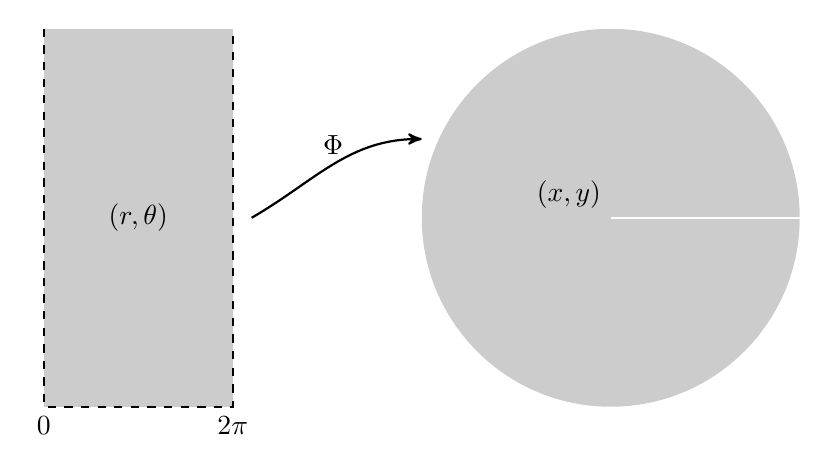
\begin{tikzpicture}[>=stealth']
        \def\size{2.4};
        \fill[gray!40] (-\size/2, -\size) rectangle (\size/2, \size);
        \draw[dashed, thick] (-\size/2, \size) -- (-\size/2, -\size) node[below] {$0$} -- (\size/2, -\size) node[below] {$2\pi$} -- (\size/2, \size);
        \fill[gray!40] (2.5*\size, 0) circle (\size);
        \draw[white, thick] (2.5*\size, 0) -- (3.5*\size, 0);
        \draw node at (0, 0) {$(r, \theta)$} node[above left] at (2.5*\size, 0) {$(x, y)$};
        \draw[thick] (0.6*\size, 0) edge[out=30, in=180, ->] node[above] {$\Phi$} (1.5*\size, 1);
    \end{tikzpicture}
    \caption{坐标变换的几何直观}
    \label{fig:coordinate-transformation}
\end{figure}

\begin{example}{坐标变换}{}
    对于定义区域 $\Omega_1$ 和 $\Omega_2$ 如下:
    \[\Omega_1 = \mathbf{R}^2\setminus\{(x, y) \mid x\geqslant 0, y = 0\},\enspace \Omega_2 = \mathbf{R}_{>0}\times (0, 2\pi) = \{(r, \theta) \mid r>0, \theta\in(0, 2\pi)\}.\]
    我们熟悉的坐标变换 $x = r\cos\theta$,$y = r\sin\theta$ 就可以写成 \[\Phi\colon \Omega_2\to\Omega_1,\enspace \Phi(r, \theta) = (r\cos\theta, r\sin\theta).\]
    如\autoref{fig:coordinate-transformation} 所示. 由于在 $\Omega_1$ 上我们给定了 $(x, y)$ 作为坐标,在$\Omega_2$ 上我们给定了 $(r, \theta)$ 作为坐标,所以我们可以使用 Jacobi 矩阵表示上述映射的微分
    \[
        \mathrm{d}\Phi = J\Phi = \begin{pmatrix}
            \dfrac{\partial x}{\partial r} & \dfrac{\partial x}{\partial \theta} \\[2ex]
            \dfrac{\partial y}{\partial r} & \dfrac{\partial y}{\partial \theta}
        \end{pmatrix} = \begin{pmatrix}
            \cos\theta & -r\sin\theta \\
            \sin\theta & r\cos\theta
        \end{pmatrix}
    \]
    根据反函数定理,这个映射当然是可逆的.
\end{example}

这个例子告诉我们:坐标变换允许我们将被积区域进行变换,比如将圆或球转化成一个矩形,这样就可以极大简化运算. 更确切来说,对于原被积区域 $\Omega$ 上的函数 $f$,我们可以定义一个映射 $\varphi\colon \Sigma \to \Omega,\enspace \varphi(\Sigma) = \Omega$,使得我们只需要在现被积区域 $\Sigma$ 对复合函数 $f\circ\varphi$ 进行积分,函数的复合保证了积分区域转换的合法性,但是我们并不可以草率进行$\displaystyle\int\limits_{\Omega}f\,\mathrm{d}x = \int\limits_{\Sigma}f\circ \varphi\,\mathrm{d}x$ 的计算,因为对于 $\Omega$ 上的某一块体积元 $\sigma$,对与 $f$ 与坐标变换 $\varphi$ 下对应的 $\Sigma$ 上的体积元 $\sigma'$ 的体积并不一定相等,就好像对于上面例子中,将圆转化为矩形一样. 那么体积究竟变化了多少呢?这就是下面重积分换元法将要讨论的事情了.

下面,我们首先考虑坐标变换为线性映射的情况,再使用微分学的基本手法对一般的坐标变换做线性化并且估计误差.

\begin{enumerate}[label=(\arabic*)]
    \item 平移变换. 设 $v_0$ 为一个固定的向量,考虑仿射线性变换$\varphi\colon \mathbf{R}^n\to \mathbf{R}^n$,$\varphi(x) = x + v_0$. 而矩形的体积显然是满足平移不变性的,对于一个可求体积的矩形 $A\subset \mathbf{R}^n$,$\varphi(A)\subset \mathbf{R}^n$当然也是可求体积的,并且体积不变.

    \item 伸缩变换. 设 $\lambda_i\in\mathbf{R}\enspace(1\leqslant i\leqslant n)$,我们考虑线性映射 $\varphi\colon \mathbf{R}^n\to \mathbf{R}^n$ ,
          \[\varphi(x_1, x_2, \ldots, x_n) = (\lambda_1x_1, \lambda_2x_2, \ldots, \lambda_nx_n),\enspace (x_1, x_2, \ldots, x_n)\in \mathbf{R}^.\]
          矩形 $A = [a_1, b_1]\times [a_2, b_2]\times \cdots\times [a_n, b_n]$ 在 $\varphi$ 下的像仍为矩形,且体积为\[ \nu(\varphi(A)) = \vert\lambda_1\vert \vert\lambda_2\vert \cdots\vert\lambda_n\vert \nu(A) = \lvert \det\varphi\rvert \nu(A).\]

          将矩形 $A$ 换成一般的可求体积的图形,上述公式仍然成立,这可以根据下面的覆盖引理得出:

          \begin{lemma}{第一覆盖引理}{}
              设 $A$ 为 $\mathbf{R}^n$ 中的可求体积的有界集合,则任给 $\varepsilon > 0$,存在有限个矩形 $\{I_i\}$ 与 $\{J_j\}$ 使得
              \[\bigcup_i I_i\subset A\subset \bigcup_i J_j; \enspace \sum_i \nu(I_i) + \varepsilon > \nu(A) > \sum_j \nu(J_j) - \varepsilon.\]
              其中 $\{I_i\}$、$\{J_i\}$ 的内部分别互不相交.
          \end{lemma}

          \begin{figure}[h]
              \centering
              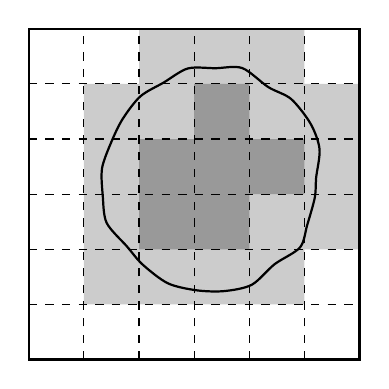
\begin{tikzpicture}[scale=0.7]
                  \pgfmathsetseed{42}

                  \fill[gray!40] (1, 1) -- (1, 5) -- (2, 5) -- (2, 6) -- (5, 6) -- (5, 5) -- (6, 5) -- (6, 2) -- (5, 2) -- (5, 1) -- cycle;
                  \fill[gray!80] (2, 2) -- (2, 4) -- (3, 4) -- (3, 5) -- (4, 5) -- (4, 4) -- (5, 4) -- (5, 3) -- (4, 3) -- (4, 2) -- cycle;

                  \draw[dashed] (0, 0) grid (6, 6);
                  \draw[thick] (0, 0) rectangle (6, 6);

                  \begin{scope}[shift={(3.3, 3.3)}]
                      \path[draw, thick] plot[domain=0:350, smooth cycle] (\x:1.9+0.2*rnd);
                  \end{scope}
              \end{tikzpicture}
              \caption{第一覆盖引理}
          \end{figure}

          \begin{proof}
              对于一个包含 $A$ 的一个矩形 $I$,首先可以定义一个示性函数 $\chi_A$,满足
              \[\chi(x) = \begin{cases}
                      1, & x\in A,    \\
                      0, & x\notin A.
                  \end{cases}\]
              这样 $A$ 的体积就可以表示为 $\nu(A) = \displaystyle\int_I\chi_A$. 因此对于任意的 $\varepsilon >0$,存在 $I$ 的分割 $\pi = \{I_{ij}\}$ 使得\[\left\lvert \sum_{ij}\chi_A(\xi_{ij})\nu(I_{ij}) - \nu(A)\right\rvert < \varepsilon,\enspace \forall \xi_{ij}\in I_{ij}.\]
              根据示性函数的定义,有 \[\sum_{ij}\inf_{\xi_{ij}\in I_{ij}}\chi_A(\xi_{ij})\nu(I_{ij}) = \sum_{I_{ij}\subset A}\nu(I_{ij}),\]
              所以,对于分割 $\pi$ 就有 \[\nu(A) - \varepsilon < \sum_{I_{ij}\subset A}\nu(I_{ij}) \leqslant \nu(A).\]
              同理可以有 \[\sum_{ij}\sup_{\xi_{ij}\in I_{ij}}\chi_A(\xi_{ij})\nu(I_{ij}) = \sum_{I_{ij}\cap A\neq \varnothing}\nu(I_{ij}),\]
              此时就有 \[\nu(A) < \sum_{I_{ij}\cap A\neq \varnothing}\nu(I_{ij}) < \nu(A) + \varepsilon.\]
              这就证明了第一覆盖引理,其中结论中的 $\{I_i\}$ 是 $I_{ij}\subset A$ 的那些 $I_{ij}$,$\{J_j\}$ 是 $I_{ij}\cap A\neq \varnothing$ 的那些 $I_{ij}$.
          \end{proof}

          这个证明的一个副产品就是:这些内部与 $\partial A$ 有非空交集的矩形的体积之和不会超过 $2\varepsilon$,这个结论也不失为一个良好的放缩.

    \item 正交变换. 正交变换就是我们所说的实数域上的等距同构. 对于正交变换 $O\in \mathcal{L}(\mathbf{R}^n)$ 其矩阵表示为 $O_M$,那么就有 $O_MO^\mathrm{T}_M = O_M^\mathrm{T}O_M = I_n$. 正交变换保持向量的模长不变,那么很自然的一点就是,我们可以大胆推断正交变换保持可求体积集合的体积不变,我们下面证明这一点. 首先需要第二覆盖引理.

          \begin{lemma}{第二覆盖引理}{}
              设 $A$ 是 $\mathbf{R}^n$ 中的可求体积的有界集合,则任给 $\varepsilon>0$,存在有限个 $n$ 维球体 $\{B_i\}$ 和 $\{B^j\}$,使得 \[\bigcap_iB_i\subset A \subset \bigcup_jB^j;\enspace \sum_j\nu(B^j) - \varepsilon < \nu(A) < \sum_j\nu(B_i) + \varepsilon,\]
              其中 $\{B_i\}$ 的内部互不相交.
          \end{lemma}

          \begin{figure}[h]
              \centering
              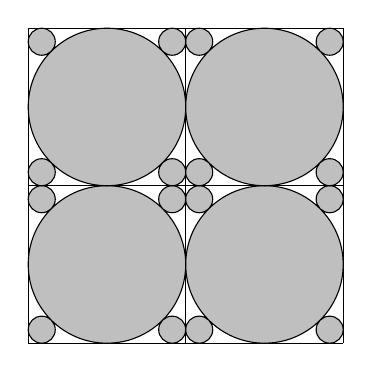
\begin{tikzpicture}[scale=2]
                  \draw (0, 0) grid (2, 2);
                  \foreach \i in {0.5, 1.5}
                      \foreach \j in {0.5, 1.5}
                          \draw[fill=gray!50] (\i, \j) circle (0.5)
                              \foreach \k in {45, 135, 225, 315} {($(\i, \j) + (\k:{sqrt(2)/(sqrt(2)+1)})$) circle ({(sqrt(2)-1)/(2+2*sqrt(2))})};
              \end{tikzpicture}
              \caption{第二覆盖引理}
          \end{figure}

          \begin{proof}
              首先设 $\nu(A)>0$. 我们先取一个矩形 $I = \left[a, b\right]^n$ 使得 $A\subset I$. 将 $I$ 作 $m^n$ 等分,当 $m$ 充分大的时候,完全包含于 $A$ 的小矩形 $\{I_i^1\}$ 的体积之和满足条件 \[\sum_i\nu(I_i^1) > \frac12\nu(A).\]
              矩形 $I_i^1$ 的内接球记为 $B_i^1$,记半径为 $1$ 的 $n$ 维球的体积为 $\omega_n$,根据球体的体积公式或者伸缩变换的结果,我们有 \[\sum_i\nu(B_i^1) = \frac{\omega_n}{2^n}\sum_i\nu(I_i^1) > \frac{\omega_n}{2^{n+1}}\nu(A).\]
              记 \[q = 1 - \frac{\omega_n}{2^{n+1}}\in(0, 1).\]
              由于 $A$ 与 $B_i$ 均可求体积,所以 $A \setminus \bigcup_iB_i^1$ 自然也可求体积(为什么?),因此 \[ 0 < \nu\left(A \setminus \bigcup_iB_i^1\right) < q\nu(A).\]
              我们对 $A\setminus \bigcup\limits_iB_i^1$ 重复上述过程,可以得到包含于 $A\setminus \bigcup\limits_iB_i^1$ 有限个小球体 $\{B_{i'}^2\}$ 使得 \[0 < \nu\left(A\setminus \bigcup_iB_i^1\setminus \bigcup_{i'}B_{i'}^2\right) < q\nu\left(A\setminus \bigcup_iB_i^1\right) < q^2\nu(A).\]
              将这一部分不断重复下去,对于任意的 $\varepsilon > 0$,由于 $q^k\to 0\enspace (k\to \infty)$,所以当 $k$ 充分大的时候,我们就得到内部互不相交的有限个 $n$ 维球体 $\{B_i\}$ 使得 \[0 < \nu\left(A\setminus \bigcup_iB_i\right) < q^k\nu(A) < n^{-n/2}\frac{\varepsilon}{2}.\]
              现在考虑对于 $\overline{A} = A\setminus \bigcup\limits_iB_i$,仍然考虑矩形 $I$ 的 $m^n$ 等分,当 $m$ 充分大的时候,存在着覆盖 $\overline{A}$ 的小矩形 $\{I^j\}$ 使得 \[\sum_j\nu(I^j) < \nu(\overline{A}) + n^{-n/2}\frac{\varepsilon}{2} < n^{-n/2}\varepsilon.\]
              矩形 $I^j$ 的外接球记为 $B_2^j$,那么就有 \[\sum_j\nu(B_2^j) = \frac{\omega_nn^{n/2}}{2^n}\sum_j\nu(I^j) < \frac{\omega_nn^{n/2}}{2^n}n^{-n/2}\varepsilon \leqslant \varepsilon.\]
              这就说明了 $\{B_i, B_2^j\}$ 就是覆盖 $A$ 的 $n$ 维球体,注意到最后一段的证明对于体积为零的情形同样适用,这就完成了第二覆盖引理的证明.
          \end{proof}

          注意,尽管我们通过两个覆盖引理刻画出了可求体积图形的性质,简单定义了一个粗糙的 Jordan ``测度'',但是我们仍然需要谨记:``有限个''这个性质在这里是至关重要的. 更加严格的测度论可以将其推广到 ``可数个'',可以在实分析等课程中学习.

          \begin{theorem}{}{}
              正交变换保持体积不变.
          \end{theorem}

          \begin{proof}
              注意到正交变换将 $n$ 维球映为 $n$ 维球,且球的半径不变,进而其体积不变. 根据第二覆盖引理,正交变换将零体积映为零体积集. 再注意到正交变换将集合的边界点映射为边界点,内点映射为内点,因此将可求体积的集合映为可求体积的集合. 再由覆盖引理及其正交变换保持球体体积变则可知正交变换保持可求体积的集合的体积不变.
          \end{proof}

    \item 一般的线性变换. 设 $\varphi\colon \mathbf{R}^n\to \mathbf{R}^n$ 为线性映射,在 $\mathbf{R}^n$ 的标准基下可以表示为 $n$ 阶方阵,这个方阵仍然记为 $\varphi$. 对于 $\mathbf{R}^n$ 中的可求体积的有界集合 $A$,我们考虑在 $\varphi$ 下的像 $\varphi(A)$. 首先,如果 $\det\varphi = 0$,那么 $\varphi$ 就将 $A$ 压缩成了被某一个超平面包含的集合,这样的集合体积为 $0$,所以我们只考虑 $\det\varphi\neq 0$ 的情况. 这时候 $\varphi\varphi^\mathrm{T}$ 就是正定对称矩阵,根据实谱定理,其可以对角化并且其特征值都大于零,所以其有一个正的平方根 $P$,这样 $\varphi\varphi^\mathrm{T}$ 就可以写为 \[\varphi\varphi^\mathrm{T} = P^2,\]
          其中 $P$ 当然也是正定对称的,且 $\det P = \lvert\det\varphi\rvert$. 这允许我们构造一个正交矩阵 $O = P^{-1}\varphi$,读者可以自行验证它是正交的.

          停下来看一下正定对称矩阵 $P$ 的性质:其对应的线性映射是一个正且自伴的线性映射,我们将其对角化为 $P = O\,\diag(\lambda_1, \lambda_2, \ldots, \lambda_n) O^\mathrm{T}$,其中 $\lambda_i > 0,\enspace 1\leqslant i\leqslant n$,且 $O$ 是一个正交变换. 根据正交变换与伸缩变换的结果,我们得到 \[\nu(P(A)) = (\det P)\nu(A).\]
          结合上面的分析,我们将一个非退化的线性映射 $\varphi$ 分解为一个正交变换与一个正定自伴映射,这就表明如果 $A$ 是可求体积的图形,那么 $\varphi(A) = P(O(A))$ 也是可求体积的,且有 \[\nu(\varphi(A)) = \nu(P(O(A))) = (\det P)\nu(O(A)) = (\det P)\nu(A) = \lvert\det\varphi\rvert \nu(A).\]
\end{enumerate}
简而言之,我们将上述分析总结为下面的定理:

\begin{theorem}{}{}
    对于一般的线性映射 $\varphi\colon \mathbf{R}^n\to \mathbf{R}^n$,与一个可求体积的图形 $A$,其像 $\varphi(A)$ 也是可求体积的,且有 \[\nu(\varphi(A)) = \lvert\det\varphi\rvert \nu(A).\]
\end{theorem}

现在我们要考虑比线性映射更一般的映射,根据``连续可微映射在某一点的局部性质与其在该点的微分的性质相同''这一核心原理,我们可以猜测对于某一点 $p$,如果 $\det J\varphi(p)\neq 0$,对于 $p$ 附近的一个非常小的可求体积的图形 $A$,有 $\nu(\varphi(A)) = \lvert\det J\varphi(p)\rvert \nu(A)$. 对这样的一个个小的面积元进行积分,就是重积分换元法的核心想法. 下面我们给出详细的证明.

设 $D\subset \mathbf{R}^n$ 为开集,$\varphi\colon D\to \mathbf{R}^n$ 为 $C^1$ 映射,根据拟微分中值定理,我们可以知道 $\varphi$ 是一个局部 Lipschitz 映射,也就是任取一个有界闭集 $P\subset D$ 与点 $x, y\in P$,存在 $\rho > 0$ 使得 \[\vert \varphi(x) - \varphi(y)\vert \leqslant \Vert J\varphi(\xi)\Vert \vert x - y\vert \leqslant \rho \vert x - y\vert.\]
所以下面讨论的主题就是如何对可求体积的集合 $A$ 在这样一个局部 Lipschitz 映射下的像 $\varphi(A)$ 的体积进行估计.

\begin{lemma}{}{}
    设 $\varphi\colon\mathbf{R}^n\to \mathbf{R}^n$ 为一个局部 Lipschitz 映射,亦即满足\[\Vert \varphi(x) - \varphi(y)\Vert \leqslant \rho \Vert x - y\Vert,\enspace \forall x, y\in\mathbf{R}^n.\]
    对于一个可求体积的集合 $A\subset \mathbf{R}^n$,如果 $A$ 为零测集,那么 $\varphi(A)$ 也是零测集;如果 $A$ 与 $\varphi(A)$ 都是可求体积的,就有 $\nu(\varphi(A)) \leqslant \rho^n\nu(A)$.
\end{lemma}

\begin{proof}
    设 $A$ 是零测集,则任给 $\varepsilon > 0$,存在至多可数个球体 $B_i = B_{r_i}(x^i)$ 使得 \[A\subset \displaystyle\bigcup_{i\geqslant 1}B_i,\enspace \sum_{i\geqslant 1}\nu(B_i) = \sum_{i\geqslant 1}\omega_n r_i^n < \varepsilon.\]
    由 $\varphi$ 是局部 Lipschitz 的可以得出 $\varphi(B_i) \subset B_{\rho r_i}(\varphi(x^i))$,所以 \[\sum_{i\geqslant 1}\nu(B_{\rho r_i}(\varphi(x^i))) = \sum_{i\geqslant 1}\omega_n (\rho r_i)^n = \rho^n\sum_{i\geqslant 1}\omega_n r_i^n < \rho^n\varepsilon.\]
    这就说明 $\varphi(A)$ 也是零测集.

    设 $A$ 和 $\varphi(A)$ 都是可求体积的,我们使用第二覆盖引理,对于任给的 $\varepsilon > 0$,存在有限个可以覆盖 $A$ 的 $n$ 维球体 $\{B_{r_j}^j\}$ 使得 \[\sum_j\omega_n r_j^n < \nu(A) + \varepsilon.\]
    所以此时 $\varphi(A)$ 被 $\{B_{\rho r_j}^j\}$ 覆盖,因此 \[\nu(\varphi(A))\leqslant \sum_{j}\omega_n (\rho r_j)^n = \rho^n\sum_j\omega_n r_j^n < \rho^n(\nu(A) + \varepsilon).\]
    通过 $\varepsilon$ 的任意性可以得出 $\nu(\varphi(A)) \leqslant \rho^n\nu(A)$.
\end{proof}

事实上,通过反函数定理,如果 $J\varphi$ 处处非退化,那么 $\varphi$ 将内点映射为内点,这就说明如果 $A$ 可求体积,并且 $\overline{A}\subset D$,那么我们对 $\partial \varphi(A)$ 进行放缩:\[\partial \varphi(A) = \overline{\varphi(A)}\setminus \varphi(A)^{\circ} \subset \varphi(\overline{A})\setminus \varphi(A^{\circ}) \subset \varphi(\partial A),\]
由 $A$ 可求体积可以得到 $\partial A$ 是零测集,所以 $\varphi(\partial A)$ 也是零测集,$\partial \varphi(A)$ 仍是零测集,所以 $\varphi(A)$ 就可求体积. 上面的定理只不过给出了 $\varphi(A)$ 体积的一个简单刻画,我们下面将 $\varphi$ 进行线性化并且进行误差估计. 取 $\delta > 0$ 使得 $K = \{x \mid d(x, A) \leqslant \delta\} \subset D$,并记 $C = \max\limits_{x\in K}\Vert J\varphi(x)\Vert$,回忆先前对线性映射与其线性化的映射之间的误差估计,我们可以直接得到下面引理:

\begin{lemma}{}{}
    沿用上面的记号,任给 $\varepsilon >0$,存在 $0<\eta <\delta$,使得当 $x\in A$,$d(x', x)\leqslant \eta$ 时,有 \[\Vert \varphi(x') - \varphi(x) - J\varphi(x)(x' - x)\Vert\leqslant \varepsilon\Vert x' - x\Vert.\]
\end{lemma}

\begin{lemma}{}{}
    沿用上面的记号,则当 $B\subset A$ 可求体积且 $d(B) < \eta$ 时,有 \[\nu(\varphi(B)) \leqslant \left(\lvert \det J\varphi(x)\rvert + O(\varepsilon)\right)\nu(B),\enspace x\in B.\]
\end{lemma}

\begin{proof}
    我们考虑线性变换 $L(y) = \left[J\varphi(x)\right]^{-1}(y - \varphi(x)) + x$ 并记 $F(y) = \varphi(y) - \varphi(x) - J\varphi(x)(x'-x)$,则 \[L\circ\varphi(x') = \left[J\varphi(x)\right]^{-1} F(x') + x'.\]
    于是当 $x', x''\in B_\eta(x)$ 的时候,\[L\circ\varphi(x') - L\circ\varphi(x'') = \left[J\varphi(x)\right]^{-1} (F(x') - F(x'')) + (x' - x'')\leqslant (1 + C\varepsilon)\Vert x' - x''\Vert.\]
    通过 $B\subset B_\eta(x)$ 可以得到 $\nu(L\circ\varphi(B)) \leqslant (1 + C\varepsilon)^n\nu(B)$,所以\[\nu(\varphi(B)) = \frac{\nu(L\circ\varphi(B))}{\lvert \det L\rvert}\leqslant \lvert \det J\varphi(x)\rvert \cdot (1 + C\varepsilon)^n\nu(B) = \left(\lvert \det J\varphi(x)\rvert + O(\varepsilon)\right)\nu(B).\]
    这样就得到了证明.
\end{proof}

\begin{theorem}{重积分换元法}{}
    设 $\varphi\colon D\to \mathbf{R}^n$ 为 $C^1$ 的一个单射,且 $J\varphi$ 处处非退化. 设 $A\subset D$ 为可求体积的集合,$\overline{A}\subset D$,$f$ 在 $\varphi(A)$ 上可积,那么\[\int_{\varphi(A)}f = \int_A f\circ \varphi\lvert \det J\varphi\rvert.\]
    特别地,\[\nu(\varphi(A)) = \int_A \lvert \det J\varphi\rvert.\]
\end{theorem}

\begin{proof}
    根据第一覆盖引理,不妨设 $A$ 为一个矩形,且 $f$ 非负,对于 $A$ 的任意一个分割 $\pi = \{A_{ij}\}$,我们有\[\int_{\varphi(A)}f = \sum_{i, j}\int_{\varphi(A_{ij})}f \leqslant \sum_{i, j}[\sup\limits_{\varphi(A_{ij})}f]\nu(\varphi(A_{ij})).\]
    对于任意的 $\varepsilon$ 当分割充分细,使得 $d(A_{ij})$ 小于某一个 $\eta$ 时,由上述的引理我们知道\[\int_{\varphi(A)}f \leqslant \sum_{i, j}\sup\limits_{A_{i, j}}(f\circ\varphi) \lvert\det J\varphi(\xi_{ij})\rvert \nu(A_{ij}) + O(\varepsilon) = \int_{A}f\circ\varphi\lvert\det J\varphi\rvert + O(\varepsilon).\]
    令 $\varepsilon\to0^+$ 可以得到\[\int_{\varphi(A)}f\leqslant \int_A f\circ\varphi\lvert\det J\varphi\rvert.\]
    根据反函数定理,$\varphi\colon D\to \varphi(D)$ 是可逆的,所以我们对于 $\varphi^{-1}$ 与 $\displaystyle\int_{A}f\circ\varphi\lvert\det J\varphi\rvert$ 进行类似的论证,可以得到 \[\int_{A}f \circ \varphi\lvert \det J\varphi\rvert \leqslant \int_{\varphi(A)}f\circ \varphi\circ\varphi^{-1}\lvert\det J\varphi\rvert \cdot\lvert \det J\varphi^{-1}\rvert  = \int_{\varphi(A)}f.\]
    综上所述,我们有\[\int_{\varphi(A)}f = \int_{A}f\circ\varphi\lvert\det J\varphi\rvert.\]这就完成了证明.
\end{proof}

这样,我们其实可以发现:重积分换元法的核心想法其实是研究\textbf{可求体积的图形在某一个映射下的体积是如何变化的}. 以这个想法为主线,配合\textbf{连续可微映射在某一点的局部性质与其在该点的微分的性质相同}这一核心原理,从线性映射到误差估计,我们就完成了重积分换元法的证明.

\vspace{2ex}
\centerline{\heiti \Large 内容总结}

\vspace{2ex}
\centerline{\heiti \Large 习题}

\vspace{2ex}
{\kaishu 但是,因为我将这些东西视作不仅是一个“量”,而且是一个“简单量”。也有其它的量是复合而成的,并且相对于其它的复合量相差一些简单量的加和。这些量通过更高级的形式的加和形成。}
\begin{flushright}
    \kaishu
    —— H. 格拉斯曼(Hermann Grassmann)
\end{flushright}

\centerline{\heiti A组}
\begin{enumerate}
    \item % Schatten 范数 是 范数
          %   设 $A$ 为 $n$ 阶矩阵,定义 $A$ 的 Schatten 范数为 $\Vert A\Vert_s = \left(\sum_{i=1}^n\sigma_i^s\right)^{1/s}$,其中 $\sigma_i$ 为 $A$ 的奇异值. 证明 $\Vert A\Vert_s$ 是一个范数.
\end{enumerate}

\centerline{\heiti B组}
\begin{enumerate}
    \item
\end{enumerate}

\centerline{\heiti C组}
\begin{enumerate}
    \item
\end{enumerate}

\LUchapter{范畴论视角下的线性代数}

% 关于代数学的历史,最值得一读的文献大概是 J. Derbyshire 的 \emph{Unknown Quantity: A Real and Imaginary History of Algebra}.这本书的写作风格轻松明快,不难卒读,其中历数的历史,笔者在此不再赘述. 而由于现代代数学卷帙浩繁,难以尽数,而且其中的大部分主题也远超笔者心力之所能及,在这里,仅仅就一些主要趋势泛泛而谈,有识见的读者可以自行翻阅文献,不必为笔者为方便理解所作的简化以及本身不完整的理解所累.

% 按照笔者的思路,我们将首先正式引入范畴论.在范畴论的框架下,接下来我们要考虑的是代数与拓扑之间的联系,这会将我们引向两个截然不同的方向:同伦论(homotopy theory)和凝聚态数学(condensed mathematics).前者相较后者历史较为悠久,正好够我们历数从 1950s 到现代的一些发展;后者则方兴未艾,可供读者一窥当代数学家的风貌. 至于一些未被纳入此框架的探讨和研究,代数数论将作为最后的讨论的切入口.还有一些剩下的,例如群论、环论、表示论等主题的发展,则只能付之阙如了.

% 当然,还有一个被遗落的庞大的专题,就是在 Derbyshire 的书中开了个头的代数几何. 这一部分的探讨笔者无力完成,只能在此稍作提示——不过,在同伦论的部分中,我们也会见到其中的许多重要人物. 这个专题几乎是当代数学的前沿核心,但也正因为其核心地位,对它所作的任何不由杰出人物写下的讨论都显得有些不足,而且其研究所需的前置知识也远非本书所能及. 因此,在此我们只能无奈将其抛下,这并非轻视其重要性的表现.

这是本书的最后一章,也是最后一个未竟专题. 一切旅程都有终点,线性代数也不例外. 但是,终点同时也是一个起点,因此,在这里,我们将要引入现代数学中必不可少的一套语言——范畴论语言,并且使用这种方式来重述线性代数的一些概念,为本书画上一个句号. 可惜的是,因为篇幅有限,在这里不能重现利用范畴语言完成的全书所有内容的推导,但是我们会尽量走的远一些,同时也轻松一些. 在读者的代数基础尚且不算充足的时候,这一节的内容看起来可能有些抽象. 但如果在现代数学的路上走出更远,回头再来用这里的内容印证自己所学,相信读者依然会有所收获,这也就是未竟专题的未竟意义之所在.

在范畴语言引入之初,其提出者之一,Mac Lane 曾经下过一个断言. 他说,范畴论没有定理. 这是因为范畴论归根结底看起来只是一种“讲法”,正如我们在标题中所言,是一种“重述”,而非一套完全新颖的理论. 但是,这个断言很快就被打破了. 从本节会提及的 Yoneda 引理到本节不可能提及的 Freyd-Mitchell 嵌入定理,范畴论本身也逐渐发展成了一个生机勃勃的学科,并隐隐有成为数学基础的有力竞争者的趋势. 因此,最后,我们也希望读者思考,数学到底是什么?它是一种如范畴论所说,对对象和关系的研究,还是一种逻辑推导,抑或是一种直觉的形式化?如果读者在此方面有所意识,那么在未竟专题中走过的路也就都是有价值的.

\section{范畴、函子、自然变换}

范畴论的引入来自于 Samuel Eilenberg and Saunders Mac Lane \emph{General theory of natural transformations}, Trans. AMS, 58, p.p.: 231-294 (1945). 我们在此以现代的语言重述其概念,下面我们要呈现其中的三个核心定义:范畴、函子、自然变换.

\begin{definition}{}{}
    称以下资料为一个\term{范畴},记作 $\cC$:
    \begin{enumerate}
        \item 一族元素,每个元素称为其中的\term{对象},这一个族记作 $\Ob(\cC)$;我们将 $A \in \Ob(\cC)$ 简记作 $A \in \cC$;
        \item 一族 $A$ 到 $B$ 的箭头或者\term{态射} $\Hom_\cC (A, B)$,对于 $\Ob(\cC)$ 中的任意两个元素 $A, B \in \cC$,满足如下条件:
              \begin{enumerate}
                  \item 如果 $A, B, C \in \cC, \alpha \in \Hom_\cC (A, B), \beta \in \Hom_\cC (B, C)$,则存在复合 $\beta \circ \alpha \in \Hom_\cC(A, C)$;
                  \item 对于任意$D \in \cC, \gamma \in \Hom_\cC (C, D)$,都有\[
                            \gamma \circ (\beta \circ \alpha)= (\gamma \circ \beta) \circ \alpha;
                        \]
                  \item $\Hom_\cC (A, A)$ 中必有一个恒同元素,记作 $\id_A$,使得对于任意的$f \in \Hom_\cC (B, A)$,
                        \[\id_A \circ f = f \circ \id_B \]
              \end{enumerate}
    \end{enumerate}
\end{definition}

对这个定义,需要进行一些说明. 我们用“一族”的地方所指的未必是“一个集合”. 这是为了避免一些集合论上的麻烦,出现例如集合的集合之类的问题. 在范畴不会引起误会的情况下,我们将 $\Hom_\cC (A, B)$ 简记成 $\Hom (A, B)$,其中的元素 $f$ 也写成 $f\colon A \to B$ 或者 $A \stackrel{f}{\to} B$.

对于本书的读者而言,最熟悉的范畴无疑是线性空间的范畴. 准确地说,是域 $\F$ 上的有限维线性空间的范畴. 我们将其记作 $\FVect_\F$. 其中的对象就是所有的有限维线性空间,两个线性空间 $V, W$ 之间的态射 $\Hom (V, W) = \mathcal{L}(V, W)$. 另一个熟悉的范畴是 $\Set$,其中的对象就是所有集合,两个集合 $S, T$ 之间的态射就是从 $S$ 到 $T$ 的映射. 但是,出于习惯考量,当后面我们提及 $\Set$ 时,涉及的态射会变成从集合 $S$ 到 $T$ 的含入映射. 当然,范畴的对象并不总是这样“类似集合”的东西,虽然目前为止,这样理解已经足够了.

最后一个说明来自于结合律. 读者可能会认为,对于定义的第二条性质,最后的要求实属多余. 但实际上,如果我们只有抽象的点和箭头,很多性质也就无从谈起. 就像我们在学习线性空间的时候,它比起集合多了许多公理,因此也多了许多性质. 结合律实际上是范畴性质之根本,正如我们在下一个定义中会看到的一样.

\begin{definition}{}{}
    设 $\cC, \cD$ 为两个范畴. 称 $F$ 为 $\cC$ 到 $\cD$ 的一个\term{函子},如果:
    \begin{enumerate}
        \item 对 $\cC$ 中的每个对象 $A$ 它指派 $\cD$ 中的一个对象 $F(A)$;
        \item 对 $\Hom_\cC (A, B)$ 中的每个态射 $\alpha$ 它指派 $\Hom_\cD (F(A), F(B))$ 中的一个态射 $F(\alpha)$,满足
              \begin{enumerate}
                  \item 对于可复合的 $\alpha, \beta$ 都有 $F(\alpha \circ \beta) = F(\alpha) \circ F(\beta)$;
                  \item 对于任意 $A \in \cC$ 都有 $F(\id_A) = \id_{F(A)}$;
              \end{enumerate}
    \end{enumerate}
\end{definition}

最简单的函子的例子是一个范畴打到自身的恒同函子,它不会改变任何东西;以及 $\FVect_\F$ 到 $\Set$ 的忘却函子,它直接抛掉线性空间中的代数结构,只留下里面的元素. 现在我们考虑一个不那么平凡的例子:

\begin{example}{}{}
    考虑范畴 $\FSet$ 的对象是所有的有限集,其中的态射为含入映射. 则它到 $\FVect_\F$ 有一个显然的函子,是张成函子,我们将其记作 $\spa: \FSet \to \FVect_\F$. 它将一个有限集合映到由它张成的线性空间. 实际上,也就是将 $S = \{s_1, s_2,\ldots, s_n\}$ 映到一个形式和:

    \[
        \spa S = \left\{\sum_{i = 1}^n a_i s_i: a_i \in \F\right\}
    \]

    其上的线性空间运算都是显然的. 同样不难验证它将原来的含入映射映到一个线性映射,一个含入映射总是可以被对应到一个从子空间到原空间的嵌入.
\end{example}

另一个我们早就有所暗示的例子有点不同,它长得更加奇怪. 考虑一个范畴 $\cC$ 的对偶为将其中所有箭头反转的新范畴——不难验证它依然满足结合律,我们将其记作 $\cC^\mathrm{op}$,称为它的对偶范畴. 于是,我们发现,$\FVect_\F$ 到 $\FVect_\F^\mathrm{op}$ 有一个显然的函子,即对偶函子. 在对偶空间的部分中,我们已经验证了它满足函子的定义. 在较为古老的教科书中,这种打到对偶范畴的函子被称为反变函子,而上面定义的函子被称为共变函子,因为这类称呼已经淹没在历史的浪潮中了,所以我们也不会再使用了.

最后一个概念是最核心的,实际上也是范畴论被提出的初衷. 还记得上面提到的论文的标题吗?它叫做“自然变换的一般理论”,于是,下面我们就要说明,什么是自然变换. 这看起来可能会有点抽象:

\begin{definition}{}{}
    考虑两个函子 $F, G: \cC \to \cD$. 称这两个函子之间的\term{自然变换}是一族 $\cD$ 中的态射 $\theta = \{\theta_X\}$,其中 $X \in \cC, \theta_X: F(X) \to G(X)$,使得对于所有 $\cC$ 中的态射 $f$,下图交换:

    \begin{center}
        \begin{tikzcd}
            F(X) \rar["\theta_X"] \dar["F(f)", swap] & G(X) \dar["G(f)"] \\
            F(Y) \rar["\theta_Y", swap] & G(Y)
        \end{tikzcd}
    \end{center}

    通常,我们将其记成以下形式:

    \begin{center}
        \begin{tikzcd}
            \cC \rar[bend left=50, "F"{name=U}]
            \rar[bend right=50, "G"{name=D}, swap]
            & \cD
            \arrow[Rightarrow, from=U, to=D, shorten =2pt, pos=0.5, "\theta"]
        \end{tikzcd}
    \end{center}

    并将其称作\term{2-胞腔}. 在最后一节中,我们将重新讨论这个名词的含义.

\end{definition}

也许,我们应该采取一种更直观的看法来理解这一串概念,下面的一些概念来自于拓扑学,但并不严格,仅仅是提供一个比较方便的几何直观. 实际上,对拓扑和范畴论更加熟悉之后,读者会发现这个类比背后的深意.

\begin{figure}[htb]
    \centering
    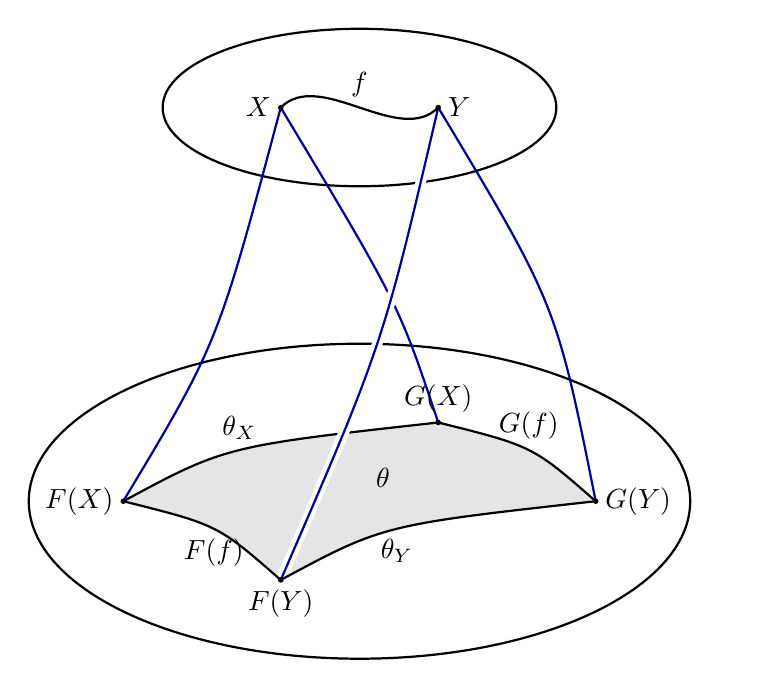
\begin{tikzpicture}
        \draw[thick] (0,3) ellipse (2.5 and 1)
        (0,-2) ellipse (4.2 and 2)
        node at (3, 3) {$\cC$}
        node at (4.7, -2) {$\cD$}
        coordinate (X) at (-1, 3)
        coordinate (Y) at (1, 3)
        coordinate (FX) at (-3, -2)
        coordinate (GY) at (3, -2)
        coordinate (GX) at (1, -1)
        coordinate (FY) at (-1, -3)
        coordinate (FX-GX-ct1) at (-1.7, -1.3)
        coordinate (FY-GY-ct1) at (0.3, -2.3)
        coordinate (FX-FY-ct1) at (-1.8, -2.3)
        coordinate (GX-GY-ct1) at (2.2, -1.3)
        coordinate (X-FX-ct1) at (-1.8, 0)
        coordinate (Y-FY-ct1) at (0.3, 0)
        coordinate (X-GX-ct1) at (0.5, 0.5)
        coordinate (Y-GY-ct1) at (2.5, 0.5);

        \fill[gray!20] (FX) .. controls (FX-GX-ct1) .. (GX) .. controls (GX-GY-ct1) .. (GY) .. controls (FY-GY-ct1) .. (FY) .. controls (FX-FY-ct1) .. (FX) -- cycle;

        \node at (0.3, -1.7) {$\theta$};

        \draw[thick] (FX) .. controls (FX-GX-ct1) .. node[above] {$\theta_X$} (GX) .. controls (GX-GY-ct1) .. node[above] {$G(f)$} (GY);
        \draw[thick,draw=blue!60!black] (X) .. controls (X-FX-ct1) .. (FX) (X) .. controls (X-GX-ct1) .. (GX);
        \draw[draw=white,double=blue!60!black,line width=1.5pt,double distance=0.8pt] (Y) .. controls (Y-FY-ct1) .. (FY);
        \draw[thick,draw=blue!60!black] (Y) .. controls (Y-GY-ct1) .. (GY);
        \draw[thick] (FX) .. controls (FX-FY-ct1) .. node[below] {$F(f)$} (FY) .. controls (FY-GY-ct1) .. node[below] {$\theta_Y$} (GY);
        \draw[thick] (X) .. controls (-.5, 3.5) and (.5, 2.5) .. node[above] {$f$} (Y);

        \node[left] at (X) {$X$};
        \node[right] at (Y) {$Y$};
        \node[left] at (FX) {$F(X)$};
        \node[right] at (GY) {$G(Y)$};
        \node[above] at (GX) {$G(X)$};
        \node[below] at (FY) {$F(Y)$};

        \foreach \point in {X, Y, FX, GX, GY, FY}
        \fill[black] (\point) circle (1pt);
    \end{tikzpicture}
    \caption{自然变换的几何直观}
    \label{fig:natural-transformation}
\end{figure}

首先,我们在一张纸上画两个面,表示两个范畴$\cC,\cD$. 在一个面上取两个点 $X, Y$,这是它上面的两个对象;然后,在另一个面上取四个点,分别表示 $F(X), F(Y), G(X), G(Y)$,即两个函子$F,G$在这两个点$X,Y$的取值. 注意,实际上两个函子分别是两个面之间的映射,如果把原像和像用线连接,展开来看的话,大概能看成是纸面上和纸面下的两张带有纹路的曲面. 然后,自然变换就是这两个曲面之间的连线$\theta$,对应到交换图上来,就是图中阴影区域的四条边. 实际上,我们的条件就是要求,这两族曲面$F, G$的结构和曲面之间的结构$\theta$都具备合适的连续性,如\autoref{fig:natural-transformation},这个东西在拓扑学中一般称为\term{同伦}.

在实践中,我们一般会称态射 $\theta_X$ 对于 $X$ 来说是自然的、典范的,或者说它满足函子性. 我们来看两个例子:

\begin{example}{}{}
    一个线性空间到某个商空间的投影映射. 考虑所有包含子空间 $U$ 的有限维线性空间. 显然,它们构成一个范畴,其间的态射定义为限制在 $U$ 上为恒同映射的线性映射,我们将这个东西记作 $\FVect_\F^U$.

    实际上,我们在说的是,考虑一个函子 $p\colon \FVect_\F^U \to \FVect_\F$ 将线性空间 $X$ 映到线性空间 $X/U$,另一个函子 $i\colon \FVect_\F^U \to \FVect_\F$ 将线性空间 $X$ 映到线性空间 $X$ 自身. 态射的映射都是显然的. 接下来,我们要表明存在一个自然变换 $\theta: i \to p$.

    现在,取任意的 $f\colon X \to Y$ 为 $\FVect_\F^U$ 中的态射,则我们需要使其交换的图表如下:

    \begin{center}
        \begin{tikzcd}
            X \rar["\theta_X"] \dar["f", swap] & X/U \dar["f/U"] \\
            Y \rar["\theta_Y", swap] & Y/U
        \end{tikzcd}
    \end{center}

    其中 $f/U$ 表示诱导的商映射,我们在不变子空间那一节中有所提及. 其中的 $\theta_X$ 和 $\theta_Y$ 就是我们通常称的典范投影,这也就是为什么这个投影被称为典范的.
\end{example}

下一个典范的结构我们也已经有所提及,它事关双对偶空间. 为了方便起见,对于函子 $F: \cC \to \cD$,我们记 $F^\mathrm{op}: \cC^\mathrm{op} \to \cD^\mathrm{op}$,它和原来的函子其实毫无差别,只有一点形式上的不同. 记对偶函子为 $-^*$,这是因为我们通常用 $V^*$ 表示对偶的空间,$f^*$ 表示对偶映射. 那么,我们就有 $(-^*)^\mathrm{op} \circ -^*$ 是典范同构. 这个事情的证明也是检查交换图,我们早已构造了这样的映射,也就是所谓的到双对偶空间的典范同构.

最后一个例子稍微有点特别,为了给出这个例子,我们需要定义一个与自然变换稍微有点不同的东西,强名之曰自然反变换\footnote{英文为 dinatural transformation,这个翻译稍微有点奇怪,但凑合用. }. 它的目标实际上是处理一些反变函子的情形,其它定义完全一致,不过它要求:$F: \cC \to \cD, G: \cC \to \cD^\mathrm{op}$,而它对应的交换图是:

\begin{center}
    \begin{tikzcd}
        F(X) \rar["\theta_X"] \dar["F(f)", swap] & G(X)\\
        F(Y) \rar["\theta_Y", swap] & G(Y) \uar["G(f)", swap]
    \end{tikzcd}
\end{center}

那么正如读者所料,我们要给出的结果就是:

\begin{example}{}{}
    不存在从一个线性空间到其对偶空间的非零自然反变换.

    现在,我们需要考虑下面的交换图:

    \begin{center}
        \begin{tikzcd}
            X \rar["\theta_X"] \dar["f", swap] & X^*\\
            Y \rar["\theta_Y", swap] & Y^* \uar["f^*", swap]
        \end{tikzcd}
    \end{center}

    我们知道,不管 $X$ 怎么取,总能取到一个 $f$ 使得 $f$ 将 $X$ 中的所有元素映到 $Y$ 中的零元,而参照我们的定义,这时的 $f^*$ 取值只有 $X^*$ 中的零元,因此,$\theta_X$ 为了让这个图交换,只能让所有元素映到零元.
\end{example}

可见在选取了合适的形式化方法之后,这些看上去无从下手的概念的证明变得无比单纯. 这实际上在表明,从一个空间到它的对偶空间不存在典范的同构.

\section{范畴论的构造}

单单是范畴、函子和自然变换显然什么都不能给出. 现在,我们无非是形式化了一些原来就已经说出的东西,顶多是最后对自然性的表述稍稍有些新意. 范畴论最核心的点实际上在于,它告诉了你很多被定义的东西实际上有其他的定义方式,这就是我们在这一节会讨论的内容.

\subsection{单态射、满态射和同构}

当我们在描述映射的时候,我们通常会讨论它是单的,满的,还是同构. 正如前面矩阵空间中关于指数映射的讨论中所表明的那样,这个性质实际上是非常不平凡的. 因此,这些性质应当在范畴论中得到恰当的推广——但是,时刻记住,现在我们的对象不同于以往我们做操作的集合,虽然我们还是能够从中汲取灵感.

先考虑集合的情况. 单射在我们看来,是如果像相同则原像相同,也就是说,每个原像集中的元素都有不同的像. 那么,就应当存在一个函数把它翻译回去,使得它在原像集上是恒同映射,也就是说:

\begin{lemma}{}{}
    考虑集合 $S, T$,一个函数 $f\colon T \to S$ 是单射当且仅当存在映射 $g\colon S \to T$ 使得 $g \circ f = \id_T$.
\end{lemma}

证明如上所述,形式化的写法留给读者,对偶地,我们就有:

\begin{lemma}{}{}
    $f\colon T \to S$ 是满射当且仅当存在映射 $g\colon S \to T$ 使得 $f \circ g = \id_S$.
\end{lemma}

而后面的这个定义是纯粹用箭头完成的,因此,它就能被推广到态射的情形:

\begin{definition}{}{}
    考虑范畴 $\cC$ 和其中的态射 $f\colon A \to B$.
    \begin{itemize}
        \item 称 $f$ 是\term{单态射},如果存在 $g\colon B \to A$ 使得 $g \circ f = \id_B$;
        \item 称 $f$ 是\term{满态射},如果存在 $g\colon B \to A$ 使得 $f \circ g = \id_A$;
        \item 称 $f$ 为\term{同构},如果存在 $g\colon B \to A$ 使得 $f \circ g = \id_A$ 且 $g \circ f = \id_B$;
        \item 如果 $A$ 和 $B$ 之间存在一个同构,则称 $A$ 和 $B$ 同构.
    \end{itemize}
\end{definition}

读者不难发现,恒同映射是一个同构. 这样的结构看上去就像一个逆元. 如果所有的态射都是同构,那么如果所有对象构成集合,态射也构成集合(这是为了避免一些集合论纷争),则我们将这个范畴构成一个\term{群胚}或者\term{广群}. 其态射集满足某种意义上的群结构. 实际上,在习题中我们会更进一步地发现相关的性质.

这里有一个麻烦的事情:同构一定既是单态射又是满态射,但既是单态射又是满态射的态射不一定是同构. 如果后者成立,则我们将这个范畴称为平衡范畴. 实际上,在通常的情形下,这个性质都是成立的.

\subsection{泛性质:始对象和终对象}

我们知道,一个范畴就是对象和箭头,那么,下面的定义看起来就很合乎情理:我们要选出箭头比较特殊的那些对象.

\begin{definition}{}{}
    称一个对象 $A \in \cC$ 为始对象,如果对于任意 $B \in \cC$ 都有 $|\Hom_\cC (A, B)| = 1$. 终对象是对偶范畴中的始对象. 如果一个对象既是始对象又是终对象,我们称其为零对象.
\end{definition}

注意,终对象的定义和始对象是完全对偶的,所以,很多时候我们其实不太区分这两种对象,它们具备的 $|\Hom_\cC (A, B)| = 1$ 的性质我们往往称为泛性质. 一般的,泛性质成立表明它实际上是一个定义性的东西:

\begin{theorem}{}{}
    所有始对象都是同构的、所有终对象都是同构的.
\end{theorem}

证明过于显然,留作读者练习. 重要的是例子:$\FVect$ 中,$\{1\}$ 是零对象. 这实际上说明了这个玩意的特殊性,但我们对它的特殊性早已习以为常. 剩下的一些例子我们会在后面的构造中一一给出——实际上,所有不太平凡的例子都要求我们构造一些更为奇特的范畴.

\subsection{Hom 函子和 Yoneda 引理}

注意到,如果 $\cC$ 和 $\cD$ 都是范畴,则 $\cC \times \cD$ 也是一个范畴,其上的对象和态射都是显然的. 我们首先考虑这样一个函子:
\[
    \Hom: \cC^\mathrm{op} \times \cC \to \Set
\]

它将对象 $(c, c')$ 映到它们之间的态射集 $\Hom_\cC(c, c')$,而将态射 $(f: c \leftarrow d, f': c' \to d')$ 映到一个 $\Hom_\cC(c, c') \to \Hom_\cC(d, d')$ 的映射,以复合的形式:
\[
    \Hom(f, f')(q: c \to c') = f' \circ q \circ f
\]

这个东西看起来乌七八糟的,但是在后面谈到张量积的时候,这个定义会体现出一个非常明显的性质. 在此,我们考虑另一种

\subsection{伴随函子}

\subsection{逗号范畴}

\subsection{和与积、极限和余极限}

\subsection{纤维化和余纤维化}

\section{幺半范畴及其性质}

\subsection{函子范畴和单子}

\subsection{Beck 单子化定理*}

\subsection{张量积}

\section{2-范畴一瞥}

\subsection{伴随和伴随}

\subsection{作为 2-极限的逗号范畴}

\subsection{走向无穷范畴:为什么我们需要套娃?}

\vspace{2ex}
\centerline{\heiti \Large 习题}

\vspace{2ex}
{\kaishu 每一门科学,当我们不是将它作为能力和统治力的工具,而是作为我们人类世代以来努力追求的对知识的冒险历程,不是别的,就是这样一种和谐,从一个时期到另一个时期,或多或少,巨大而又丰富:在不同的时代和世纪中,对于依次出现的不同的主题,它展现给我们微妙而精细的对应,仿佛来自虚空。}
\begin{flushright}
    \kaishu
    ————《收获与播种》,格罗滕迪克
\end{flushright}

\begin{enumerate}
    \item 证明以下两个态射的性质:
          \begin{enumerate}
              \item 如果 $A$ 与 $B$ 同构,那么 $A$ 与 $B$ 之间的同构映射是唯一的;
              \item 函子保持态射的单、满性质.
          \end{enumerate}
\end{enumerate}

\end{document}


\LUgroupsancheck

\makeatletter
\let\chapter\@std@chapter
\let\@std@chapter\relax
\makeatother

\backmatter
{\small
\printindex
\printindex[sym]
}

\end{document}
